% = = = = = = = = = = = = = = = = = = = = = = = = = = = = = = = = = = = = = = = = = = = = =
% P  R  E  A  M  B  L  E
% = = = = = = = = = = = = = = = = = = = = = = = = = = = = = = = = = = = = = = = = = = = = =
\documentclass[11pt]{article}
\usepackage{amsbsy, amsmath, amssymb, authblk}

%\usepackage{array} 
%\usepackage{algorithm2e}

\usepackage{booktabs, bm}
\usepackage[small,labelfont=bf,up,singlelinecheck=false]{caption}
\usepackage{cancel}
\usepackage{comment}
%\usepackage{fancyhdr}
%\usepackage[default]{lato}
\usepackage[T1]{fontenc}
\usepackage[bottom]{footmisc}
\usepackage{geometry}
\usepackage{graphicx}
\usepackage{hyperref}
%\usepackage[utf8]{inputenc}
%	\inputencoding{latin1}
%	\inputencoding{utf8}
%\usepackage{lettrine}
%\usepackage[sc]{mathpazo}
\usepackage{lmodern} % Nice fonts?
%\usepackage{mathrsfs}
\usepackage{mathtools} 
%\usepackage{marvosym} % silly bullet-point symbols (misc symbols)
%\usepackage{microtype}
\usepackage{minitoc}         % left in case it is needed elsewhere
\setcounter{secttocdepth}{5} % idem
\usepackage{etoc} % for toc before each section.
%\usepackage{multicol}
\usepackage{needspace}
\usepackage{paralist}
%\usepackage{polynom} 			% typesetting polynomial long division
%\usepackage{setspace}
%	\onehalfspacing 
\usepackage{tocloft}
\usepackage{xparse} % DeclareDocumentCommand
\usepackage[compact]{titlesec} 		% compact shrinks whitespace around section headings.
\usepackage{ulem} 				% for strikeout \sout command.
%\usepackage{verbatim}

% Muh packagez :)
\usepackage{../Packages/MathCommands}
\usepackage{../Packages/BrandonColors}
\usepackage{../Packages/BrandonBoxes}
\usepackage{../Packages/NoteTaker}
%\usepackage{../Packages/MachineLearningUtils}


%\usepackage{program}
% DL BOOK CONVENTIONS
\renewcommand\vec[2][]{\bm{#2}_{#1}}

\DeclareDocumentCommand{\slice}
	{ O{t} O{1} m }
	{\vec[\langle #2 \ldots #1 \rangle]{#3}}

\newcommand\myfig[2][0.3\textwidth]{\begin{figure}[h!]\centering\includegraphics[width=#1]{#2}\end{figure}}
\newcommand\myspace[1][]{\vspace{#1\bigskipamount}}
\newcommand\p{\Needspace{10\baselineskip} \noindent}
\newcommand\tlab[1]{\tag{#1}\label{#1}}
\newcommand\Var[1]{\mathrm{Var}\left[#1\right]}


%\usepackage{program}

\usepackage{layout} % Type \layout() anywhere to see values of layout frame.
%\usepackage{showframe} % Displays layout frame on all pages
\usepackage{marginnote}
\renewcommand*{\marginfont}{\scriptsize}

\usepackage{listings}

\definecolor{dkgreen}{rgb}{0,0.6,0}
\definecolor{gray}{rgb}{0.5,0.5,0.5}
\definecolor{mauve}{rgb}{0.58,0,0.82}

\lstset{frame=tb,
	language=Java,
	aboveskip=3mm,
	belowskip=3mm,
	showstringspaces=false,
	columns=flexible,
	basicstyle={\small\ttfamily},
	numbers=none,
	numberstyle=\tiny\color{gray},
	keywordstyle=\color{blue},
	commentstyle=\color{dkgreen},
	stringstyle=\color{mauve},
	breaklines=true,
	breakatwhitespace=true,
	tabsize=3
}

\usepackage{tikz}
\usetikzlibrary{arrows, automata, shapes, snakes, positioning}
\usetikzlibrary{bayesnet}


\titleformat*{\subsubsection}{\small\scshape}
\newcommand\subsub[1]{\Needspace{15\baselineskip}\hrule\subsubsection{#1}\hrule}
\newcommand\matgrad[2]{\nabla_{\mathbf{#2}} #1}

\newcommand\dotseq[2]{#1^{(1)}, \ldots, #1^{(#2)}}
\newcommand\rdotseq[2]{#1^{(#2)}, \ldots, #1^{(1)}} % reversed

% O{T} means "optional with default value of `T`"
% m means mandatory argument
\DeclareDocumentCommand{\vecseq}
	{ O{T} m }
	{ \{  \vec[1]{#2}, \ldots, \vec[#1]{#2}   \}  }
\DeclareDocumentCommand{\seq}
	{ O{T} m }
	{ \{ #2_1, \ldots #2_#1 \} }
	
\newcommand\QA[2]{\item \red{Q}: #1
	\begin{compactitem}
		\item \green{A}: #2
	\end{compactitem}}
	
\newcommand\myref[1]{\purple{[#1]}}

\definecolor{forgeblue}{HTML}{018C9F}
% Gray table borders
\makeatletter
\def\rulecolor#1#{\CT@arc{#1}}
\def\CT@arc#1#2{%
	\ifdim\baselineskip=\z@\noalign\fi
	{\gdef\CT@arc@{\color#1{#2}}}}
\let\CT@arc@\relax
\rulecolor{forgeblue}
\makeatother


%\setlength{\parskip}{1pt}
%\setlength{\columnseprule}{0.1pt}
%\setlength{\columnsep}{0.6cm}
%\setlength\tabcolsep{0.1cm}
\renewcommand{\arraystretch}{1.2}


\DeclareDocumentEnvironment{definition}{O{-0.5em} o}{
	\IfNoValueTF{#2}{}{\textbf{#2}}
	\vspace*{#1}
	\begin{quote}
		\itshape\small}
	{\end{quote}}

\makeatletter
\newcommand*\dotp{\mathpalette\dotp@{.5}}
\newcommand*\dotp@[2]{\mathbin{\vcenter{\hbox{\scalebox{#2}{$\m@th#1\bullet$}}}}}
\makeatother

% bluesec
\newcommand\bluesec[1]{\myspace \p \blue{#1}}

% Title
\title{\vspace{-10mm}\fontsize{24pt}{8pt}\selectfont\textbf{Fall 2016 Course Notes}\vspace*{-4mm}}
% Author
\author{Brandon McKinzie}
% Date
\date{}

% --------------------------------------------------------------
% --------------------------------------------------------------


\renewcommand\cftsecfont{\small\bfseries}
\renewcommand\cftsubsecfont{\scriptsize}
\renewcommand\cftsubsubsecfont{\scriptsize}

\renewcommand\cftsecafterpnum{\vskip-5pt}
\renewcommand\cftsubsecafterpnum{\vskip-7pt}
\renewcommand\cftsubsubsecafterpnum{\vskip-7pt}

\begin{document}
\dosecttoc
\tableofcontents

% ==================================================================================
% APPLIED MATH AND ML BASICS
% ==================================================================================
\mysection{Math and Machine Learning Basics}\label{Math and Machine Learning Basics}

\lecture{Math and Machine Learning Basics}{Linear Algebra (Quick Review) (Ch. 2)}{January 23, 2017}

\begin{itemize}
	\item For $A^{-1}$ to exist, $Ax=b$ must have \underline{exactly} one solution for every value of $b$.\marginnote{Unless stated otherwise, assume $A \in \R^{m\times n}$} Determining whether a solution exists $\forall b \in \R^m$ means requiring that the \green{column space} (range) of $A$ be all of $\R^m$. It is helpful to see $Ax$ expanded out explicitly in this way:
	\begin{align}
 		\matr{A} \vec{x} &= \sum_i x_i \matr[:,i]{A} 
 			= x_1 \begin{pmatrix} A_{1,1} \\ \vdots \\ A_{m,1} \end{pmatrix}
 				+ \cdots 
 				+ x_m \begin{pmatrix} A_{1,n} \\ \vdots \\ A_{m,n} \end{pmatrix}
 			\tlab{2.27}
	\end{align}
	\begin{compactitem}[$\rightarrow$]
		\item Necessary: $\matr{A}$ must have at least $m$ columns ($n \ge m$). (``wide''). 
		\item Necessary \textit{and} sufficient: matrix must contain at least one set of $m$ linearly independent columns. 
		\item Invertibility: In addition to above, need matrix to be \textit{square} (re: at most $m$ columns $\land$ at least $m$ columns). 
	\end{compactitem}

	\item A square matrix with linearly dependent columns is known as \green{singular}. A (necessarily square) matrix is singular if and only if one or more eigenvalues are zero. 

	% Norms
	\item A \green{norm} is any function $f$ that satisfies the following properties:\marginnote{$||x||_\infty = \max_i |x_i|$}
	\begin{align}
		f(\vec{x}) = 0 &\Rightarrow \vec{x} = \vec{0} \\
		f(\vec{x} + \vec{y}) &\le f(\vec{x}) + f(\vec{y}) \\
		\forall \alpha \in \R, ~ f(\alpha \vec{x}) &= |\alpha|f(\vec{x})
	\end{align}
	
	\item An \green{orthogonal matrix} is a square matrix whose rows are mutually orthonormal and whose columns are mutually orthonormal:\marginnote{Note that orthonorm cols implies orthonorm rows (if square). To prove, consider the relationship between $\matr{A}^T\matr{A}$ and $\matr{A}\matr{A}^T$}
	\begin{align}
		\matr{A}^T\matr{A} &= \matr{A}\matr{A}^T = \matr{I} \tlab{2.37} \\
		\matr{A}^{-1} &= \matr{A}^T \tlab{2.38}
	\end{align}
	
	\item Suppose square matrix $\matr{A} \in \R^{n \times n}$ has $n$ linearly independent eigenvectors $\{\vec{v}^{(1)}, \ldots, \vec{v}^{(n)}\}$. The \green{eigendecomposition} of $\matr{A}$ is then given by\marginnote{\underline{All} real-symmetric $\matr{A}$ have an eigendecomposition, \textbf{but it might not be unique!}}[2cm]\footnote{This appear to imply that unless the columns of $V$ are also normalized, can't guarantee that its inverse equals its transpose? (since that is the only difference between it and an orthogonal matrix)}
	\begin{align}
		\matr{A} &= \matr{V} ~  \diag{\vec{\lambda}} ~ \matr{V}^{-1} \tlab{2.40}
	\end{align}
	In the special case where $\matr{A}$ is real-symmetric, $\matr{A} = \matr{Q}\matr{\Lambda}\matr{Q}^T$. \purple{Interpretation:} $\matr{A}\vec{x}$ can be decomposed into the following three steps:
	\begin{compactitem}
		\item[1)] \textbf{Change of basis}: The vector $(\matr{Q}^T\vec{x})$ can be thought of as how $\vec{x}$ would appear in the basis of eigenvectors of $\matr{A}$. 
		\item[2)] \textbf{Scale}: Next, we scale each component $(\matr{Q}^T\vec{x})_i$ by an amount $\lambda_i$, yielding the new vector $(\matr{\Lambda}(\matr{Q}^T\vec{x}))$. \marginnote{A common convention to sort the entries of $\Lambda$ in descending order. }
		\item[3)] \textbf{Change of basis}: Finally, we rotate this new vector back from the eigen-basis into its original basis, yielding the transformed result of $\matr{Q}\matr{\Lambda}\matr{Q}^T\vec{x}$. 
	\end{compactitem}

	\item \green{Positive definite}: all $\lambda$ are positive; \green{positive semidefinite}: all $\lambda$ are positive or zero.
	\begin{compactitem}[$\rightarrow$]
		\item PSD: $\forall \vec{x}, ~~ \vec{x}^T \matr{A} \vec{x} \ge 0$
		\item PD: $\vec{x}^T \matr{A} \vec{x} = 0 ~ \Rightarrow ~ \vec{x} = \vec{0}$.\footnote{I proved this and it made me happy inside. Check it out. 
			Let $\matr{A}$ be positive definite. Then 
			\begin{align}
				\vec{x}^T \matr{A} \vec{x} &= \vec{x}^T \matr{Q} \matr{\Lambda} \matr{Q}^T \vec{x} \\
				&= \sum_i (\matr{Q}^T \vec{x})_i \lambda_i (\matr{Q}^T \vec{x})_i \\
				&= \sum_i \lambda_i (\matr{Q}^T \vec{x})^2_i 
			\end{align}
			Since all terms in the summation are non-negative and all $\lambda_i > 0$, we have that $\vec{x}^T \matr{A} \vec{x} = 0$ if and only if $(\matr{Q}^T \vec{x})_i = 0 = \vec{q}^{(i)} \cdot \vec{x}$ for all $i$. Since the set of eigenvectors $\{\vec{q}^{(i)}\}$ form an orthonormal basis, we have that $\vec{x}$ must be the zero vector. }
	\end{compactitem}

	% ------------  SVD -------------
	\item Any real matrix $\matr{A} \in \R^{m \times n}$ has a \green{singular value decomposition} of the form, \marginnote{\begin{align}
		\matr{U} &\in \R^{m \times m} \\ 
		\matr{D} &\in \R^{m \times n} \\
		\matr{V} &\in \R^{n \times n} 
		\end{align}}
	\begin{align}
		\matr{A} &= \matr{U} \matr{D} \matr{V}^T
	\end{align}
	where both $\matr{U}$ and $\matr{V}$ are orthogonal matrices, and $\matr{D}$ is diagonal. 
	\begin{compactitem}
		\item The \textbf{singular values} are the diagonal entries $\matr[ii]{D}$. 
		\item The \textbf{left(right)-singular vectors} are the columns of $\matr{U}$($\matr{V}$). 
		\item Eigenvectors of $\matr{A}\matr{A}^T$ are the L-S vectors. Eigenvectors of $\matr{A}^T\matr{A}$ are the R-S vectors. The eigenvalues of both $\matr{A}\matr{A}^T$ and $\matr{A}^T\matr{A}$ are given by the singular values squared. 
	\end{compactitem}

	\item The Moore-Penrose \green{pseudoinverse}, denoted $\matr{A}^+$, enables us to find an ``inverse'' of sorts for a (possibly) non-square matrix $\matr{A}$.\marginnote{$\matr{A}^+$ is useful, e.g., when we want to solve $\matr{A} \vec{x} = \vec{y}$ by left-multiplying each side to obtain $\vec{x} = \matr{B} \vec{y}$.\\ It is far more likely for solution(s) to exist when $\matr{A}$ is wider than it is tall.} Most algorithms compute $\matr{A}^+$ via
	\begin{align}
		\matr{A}^+ = \matr{V} \matr{D}^{+} \matr{U}^T 
	\end{align}
	
	
	\item The \green{determinant} of a matrix is $\det(\matr{A}) = \prod_i \lambda_i$. Conceptually, $|\det(\matr{A})|$ tells how much [multiplication by] $\matr{A}$ expands/contracts space. If $\det(\matr{A}) = 1$, the transformation preserves volume.
\end{itemize}

\subsub{Example: Principal Component Analysis}

\myspace
\p \blue{Task}. Say we want to apply lossy compression (less memory, but may lose precision) to a collection of $m$ points $\{\vec{x}^{(1)}, \ldots, \vec{x}^{(m)} \}$. We will do this by converting each $\vec{x}^{(i)} \in \R^n$ to some $\vec{c}^{(i)} \in \R^l$ ($l < n$), i.e. finding functions $f$ and $g$ such that:
\begin{align}
	f(\vec{x}) = \vec{c} \quad \text{and} \quad \vec{x} \approx g(f(\vec{x}))
\end{align}


\myspace
\p \blue{Decoding function ($g$)}. As is, we still have a rather general task to solve. \textit{PCA} is defined by choosing $g(\vec{c}) = \matr{D}\vec{c}$, with $\matr{D} \in \R^{n \times l}$, where all columns of $\matr{D}$ are both (1) orthogonal and (2) unit norm.

\myspace
\p \blue{Encoding function ($f$)}. Now we need a way of mapping $\vec{x}$ to $\vec{c}$ such that $g(\vec{c})$ will give us back a vector optimally close to $\vec{x}$. We've already defined $g$, so this amount to finding the optimal $\vec{c}*$ such that:
\begin{align}
	\vec{c}* &= \argmin_{\vec{c}} || \vec{x} - g(\vec{c}) ||_2^2 \\
	(\vec{x} - g(\vec{c}))^T (\vec{x} - g(\vec{c})) &= \vec{x}^T\vec{x} - 2 \vec{x}^T g(\vec{c}) + g(\vec{c})^T g(\vec{c}) \\
	\vec{c}* &= \argmin_{\vec{c}} \left[ -2 \vec{x}^T \matr{D} \vec{c} + \vec{c}^T \vec{c} \right] \\
	&= \matr{D}^T \vec{x} = f(\vec{x})
\end{align}
which means the PCA \textit{reconstruction operation} is defined as $r(\vec{x}) = \matr{D} \matr{D}^T \vec{x}$.

\myspace
\p \blue{Optimal $\matr{D}$}. It is important to notice that we've been able to determine e.g. the optimal $\vec{c}*$ \textit{for some} $\vec{x}$ because each $\vec{x}$ has a (allowably) different $\vec{c}*$. However, we use \textit{the same} matrix $\matr{D}$ for all our samples $\vec{x}^{(i)}$, and thus must optimize it over all points in our collection. With that out of the way, we just do what we always do: minimize over the $L^2$ distance between points and their reconstruction. Formally, we minimize the Frobenius norm of the matrix of errors:
\begin{align}
\matr{D}* &= \argmin_{\matr{D}} \sqrt{ 
		\sum_{i,j} \left( \vec[j]{x}^{(i)}  -   r(\vec{x}^{(i)})_j \right)^2
	  } \quad s.t. \quad \matr{D}^T \matr{D} = \matr{I}
\end{align} 

\p Consider the case of $l = 1$ which means $\matr{D} = \vec{d} \in \R^n$. In this case, after [insert math here], we obtain
\begin{align}
	\vec{d}* &= \argmax_{\vec{d}} Tr\left( \vec{d}^T \matr{X}^T \matr{X} \vec{d} \right)
	\quad s.t. \quad \vec{d}^T \vec{d} = 1
\end{align}
where, as usual, $\matr{X} \in \R^{m,n}$. It should be clear that the optimal $\vec{d}$ is just the largest eigenvector of $\matr{X}^T \matr{X}$. 


% =================================================================================
% Probability 
% =================================================================================
\lecture{Math and Machine Learning Basics}{Probability \& Information Theory (Quick Review) (Ch. 3)}{January 24}

\p \blue{Expectation}. For some function $f(x)$, $\E[x \sim P]{f(x)}$ is the mean value that $f$ takes on when $x$ is drawn from $P$. The formula for discrete and continuous variables, respectively is as follows:
\begin{align}
\E[x \sim P]{f(x)} &= \sum_x P(x) f(x) \tlab{3.9} \\
\E[x \sim P]{f(x)} &= \int p(x) f(x) \mathrm{d}x \tlab{3.10} 
\end{align}

\myspace 
\p \blue{Variance}. A measure of how much the values of a function of a random variable $x$ vary as we sample different values of $x$ from its distribution.
\begin{align}
\Var{f(x)} = \E{(f(x) - \E{f(x)})^2} \tlab{3.11}
\end{align}

\myspace
\p \blue{Covariance}. Gives some sense of how much two values are \textit{linearly} related to each other, as well as the \textit{scale} of these variables.
\begin{align}
\Cov{f(x)}{g(x)} = \E{~\left(f(x) - \E{f(x)}\right)~\left(g(x) - \E{g(x)}\right)~} \tlab{3.13}
\end{align}
\begin{compactitem}[$\rightarrow$]
	\item Large $|\Cov{f}{g}|$ means the function values change a lot and both functions are far from their means at the same time.
	\item \green{Correlation} normalizes the contribution of each variable in order to measure only how much the variables are related.
\end{compactitem}

\myspace
\p \blue{Covariance Matrix} of a random vector $\rvec{x} \in \R^{n}$ is an $n \times n$ matrix, such that
\begin{align}
\mathrm{Cov}\left[\rvec{x}\right]_{i,j}   = \Cov{x_i}{x_j} \tlab{3.14}
\end{align}
and if we want the ``sample'' covariance matrix taken over $m$ data point samples, then
\begin{align}
\Sigma &:= \frac{1}{m} \sum_{k = 1}^{m} (x_k - \bar x)(x_k - \bar x)^T
\end{align}
where $m$ is the number of data points.

\myspace
\p \blue{Measure Theory}. 
\begin{compactitem}
	\item A set of points that is negligibly small is said to have \green{measure zero}. In practical terms, think of such a set as occupying no volume in the space we are measuring (interested in). \marginnote{In $\R^2$, a line has measure zero.}
	\item A property that holds \green{almost everywhere} holds throughout all space except for on a set of measure zero.
\end{compactitem}

\myspace
\p \blue{Functions of RVs}. 
\begin{compactitem}
	\item \red{Common mistake:} Suppose $\rvec{y} = g(\rvec{x})$, and $g$ is invertible/continuous/differentiable. It is NOT true that $p_y(\rvec{y}) = p_x(g^{-1}(\rvec{y}))$. This fails to account for the distortion of [probability] space introduced by $g$. Rather, 
	\graybox{
		p_x(\rvec{x}) &= p_y(g(\rvec{x})) \bigg| \pderiv{g(\rvec{x})}{\rvec{x}}\bigg| \tlab{3.47}
	}
\end{compactitem}


\myspace
\p \blue{Information Theory}. Denote the \green{self-information} of an event $\rvec{x} = x$ to be 
\begin{align}
	I(x) \triangleq - \log P(x)
\end{align}
where $\log$ is always assumed to be the natural logarithm. We can quantify the amount of uncertainty in an entire probability distribution using the \green{Shannon entropy},
\begin{align}
	H(\rvec{x}) &= \E[\rvec{x} \sim P]{I(x)} = - \E[\rvec{x} \sim P]{\log P(x)}
\end{align}
which gives the expected amount of information in an event drawn from that distribution. Taking it a step further, say we have two separate probability distributions $P(\rvec{x})$ and $Q(\rvec{x})$. We can measure how different these distributions are with the \green{Kullback-Leibler (KL) divergence}:
\begin{align}
	D_{KL}\left( P || Q \right) &\triangleq \E[\rvec{x} \sim P]{\log \frac{P(x)}{Q(x)} } = \E[\rvec{x} \sim P]{\log P(x) - \log Q(x)}
\end{align}
Note that the expectation is taken over $P$, thus making $D_{KL}$ not symmetric (and thus not a true distance measure), since $D_{KL}(P || Q) \ne D_{KL}(Q || P)$. Finally, a closely related quantity is the \green{cross-entropy}, $H(P, Q)$, defined as:
\graybox{
	H(P, Q) &\triangleq H(P) + D_{KL}(P || Q) \\
	&= - \E[\rvec{x} \sim P]{\log Q(x)}
	}







% =================================================================================
% Numerical Computation 
% =================================================================================
\lecture{Math and Machine Learning Basics}{Numerical Computation (Ch. 4)}{January 24, 2017}

\p \blue{Some terminology}. \green{Underflow} is when numbers near zero are rounded to zero. Similarly, \green{overflow} is when large [magnitude] numbers are approximated as $\pm \infty$. \green{Conditioning} refers to how rapidly a function changes w.r.t. small changes in its inputs. Consider the function $f(\vec{x}) = \matr{A}^{-1}\vec{x}$. When $\matr{A}$ has an eigenvalue decomposition, its \textit{condition number} is
\begin{align}
\max_{i, j} \bigg| \frac{\lambda_i}{\lambda_j} \bigg| \tlab{4.2}
\end{align}
which is the ratio of the magnitude of the largest and smallest eigenvalue. When this is large, matrix inversion is sensitive to error in the input [of f(x)]. \\

\myspace
\blue{Gradient-based optimization}. Recall from basic calculus that the \green{directional derivative} of $f(\vec x)$ in direction $\vec{\hat{u}}$ (a unit vector) is defined as the slope of the function $f$ in direction $\vec{\hat u}$. By definition of the derivative, this is given by (with $\vec v := \vec x + \alpha \vec{\hat u}$)
\begin{align}
	\lim_{\alpha \rightarrow 0} \frac{f(\vec x + \alpha \vec{\hat u}) - f(\vec{x})   }{\alpha} &= \pderiv{f(\vec{x} + \alpha \vec{\hat u})}{\alpha} \bigg|_{\alpha=0} \\
	&= \sum_i \pderiv{f(\vec v)}{v_i}\pderiv{v_i}{\alpha} ~ \bigg|_{\alpha=0}  \\
	&= \sum_i (\nabla_{\vec v} f(\vec v))_i ~  u_i ~ \bigg|_{\alpha=0} \\
	&= \vec{\hat u}^T \nabla_{\vec v} f(\vec v) \bigg|_{\alpha=0} \\
	&= \vec{\hat u}^T \nabla_{\vec x} f(\vec x) \label{directional-deriv}
\end{align}
where it's important to recognize the distinction between $\lim_{\alpha \rightarrow 0}$ and \textit{setting} $\alpha$ to zero, which is denoted by $\big|_{\alpha=0}$. If we want to \textit{find} the direction $\vec{\hat u}$ such that this directional derivative is a minimum, i.e. 
\begin{align}
	\vec{\hat u}^* &= \argmin_{\vec{\hat u}, \vec{\hat u}^T \vec{\hat u} = 1} \vec{\hat u}^T \nabla_{\vec x} f(\vec x) \\
	&=  \argmin_{\vec{\hat u}, \vec{\hat u}^T \vec{\hat u} = 1} ||\vec{\hat u}||_2 ~ ||\nabla_{\vec x} f(\vec x)||_2 ~ \cos(\vec{\theta}) \\
	&= \cos(\vec{\theta})
\end{align}
and we see that $\vec{\hat u}$ points in the opposite direction as the gradient. 

\myspace
\p \blue{Jacobian and Hessian Matrices}. For when we want partial derivatives of some function f\marginnote{$f: \R^m \rightarrow \R^n$} whose input and output are both vectors. The \textbf{Jacobian matrix}\marginnote{$\matr{J} \in \R^{n \times m}$ where $J_{i,j} = \pderiv{}{x_j} f(\vec{x})_i$}[1em] contains all such partial derivatives. Sometimes we want to know about second derivatives too, since this tells us whether a gradient step will cause as much of an improvement as we would expect based on the gradient alone. The \textbf{Hessian matrix} $\matr{H}(f)(\vec{x})$ is defined such that \marginnote{The Hessian is the Jacobian of the gradient.}
\begin{align}
\matr{H}(f)(\vec{x})_{i,j} &= \pderiv{^2}{x_i\partial x_j} f(\vec{x}) \tlab{4.6}
\end{align}
The second derivative in a specific direction $\vec{\hat{d}}$ is given by $\hat{\vec{d}}^T \matr{H} \hat{\vec{d}}$\footnote{
	In the same manner that I derived equation \ref{directional-deriv}, we can derive the second derivative in a specified direction $\vec{\hat d}$:
	\begin{align}
		\ppderiv{}{\alpha} f(\vec{x} + \alpha \vec{\hat d}) \big|_{\alpha=0}
		&= \pderiv{}{\alpha} \vec{\hat d}^T \nabla_{\vec{v}} f(\vec{v}) \big|_{\alpha=0} \\
		&= \sum_i d_i \pderiv{}{\alpha} \pderiv{f(\vec v)}{v_i} ~ \big|_{\alpha=0} \\
		&= \sum_i d_i \pderiv{}{v_i} \pderiv{f(\vec v)}{\alpha} ~ \big|_{\alpha=0} \\
		&= \sum_i \sum_j d_i \pderiv{^2f(\vec v) }{v_i v_j} d_j ~ \big|_{\alpha=0} \\
		&= \vec{\hat d}^T \matr{H} \vec{\hat d}
	\end{align}
}. It tells us how well we can expect a gradient descent step to perform. How so? Well, it shows up in the second-order approximation to the function $f(\vec{x})$ about our current spot, which we can denote $\vec{x}^{(0)}$. The standard gradient descent step will move us from $\vec{x}^{(0)} \rightarrow \vec{x}^{(0)} - \epsilon g$, where $g$ is the gradient evaluated at $\vec{x}^{(0)}$. Plugging this in to the 2nd order approximation shows us how $\matr{H}$ can give information related to how ``good'' of a step that really was. Mathematically, 
\begin{align}
	f(\vec{x}) &\approx f(\vec{x}^{(0)}) + (\vec{x} - \vec{x}^{(0)})^T \vec{g} + \onehalf (\vec{x} - \vec{x}^{(0)})^T \matr{H} (\vec{x} - \vec{x}^{(0)}) \tlab{4.8} \\
	f(\vec{x}^{(0)} - \epsilon \vec{g}) &\approx f(\vec{x}^{(0)}) - \epsilon \vec{g}^T\vec{g} + \onehalf \epsilon^2 \vec{g}^T \matr{H} \vec{g} \tlab{4.9}
\end{align}
If $\vec{g}^T \matr{H} \vec{g}$ is positive, then we can easily solve for the optimal $\epsilon = \epsilon^*$ that decreases the Taylor series approximation as
\begin{align}
\epsilon^* &= \frac{\vec{g}^T\vec{g} }{\vec{g}^T \matr{H} \vec{g} } \tlab{4.10}
\end{align}
which can be as low as $1/\lambda_{max}$ (the worst case), and as high as $1/\lambda_{min}$ with the $\lambda$ being the eigenvalues of the Hessian. The best (and perhaps only) way to take what we learned about the ``second derivative test'' in single-variable calculus and apply it to the multidimensional case with $\matr{H}$ is by using the \textit{eigendecomposition of} $\matr{H}$. Why? Because we can examine the eigen\underline{values} of the Hessian to determine whether the critical point $\vec{x}^{(0)}$ is a local maximum, local minimum, or saddle point\footnote{Emphasis on ``values'' in ``eigen\underline{values}'' because it's important not to get tripped up here about what the eigenvectors of the Hessian mean. The reason for the decomposition is that it gives us an orthonormal basis (out of which we can get any direction) and therefore the magnitude of the second derivative along each of these directions as the eigenvalues.}. If all eigenvalues are positive (remember that this is equivalent to saying that the Hessian is \textbf{positive definite}!)\marginnote{The condition number of the Hessian at a given point can give us an idea about how much the second derivatives (along different directions) differ from each other}, the point is a local minimum.

\myspace
\p \blue{Constrained optimization}: minimizing/maximizing a function $f(\vec x)$ constrained to only values of $\vec x$ in some set $\mathbb{S}$. One way of approaching such a problem is to re-design the unconstrained optimization problem such that the re-designed problem's solution satisfies the constraints. For example, to minimize $f(\vec x)$ for $\vec x \in \R^2$ with constraint $||\vec x||_2 = 1$, we can minimize $g(\theta) = f([\cos\theta, \sin\theta]^T)$ wrt $\theta$, then return $[\cos\theta, \sin\theta]^T$ as the solution to the original problem.  \\

The \green{Karush-Kuhn-Tucker} (KKT) approach, a generalization of \green{Lagrange multipliers}, provides a general approach for re-designing the optimization problem, with procedure as follows:
\begin{compactenum}
	\item Find $m$ functions $g^{(i)}$ and $n$ functions $h^{(j)}$ such that your set of allowed values $\mathbb{S}$ can be written
	\begin{align}
		\mathbb{S} = \{ \vec x \mid \forall i, g^{(i)}(\vec x) = 0 \text{ and } \forall j, h^{(j)}(\vec x) \le 0   \}
	\end{align}
	The equations involving $g^{(i)}$ are called the \green{equality constraints} and the inequalities involving $h^{(j)}$ are called the \green{inequality constraints}. 
	
	\item Introduce new variables $\lambda_i$ (for the equality constraints) and $\alpha_j$ (for the inequality constraints). These are called the KKT multipliers. The generalized Lagrangian is then defined as
	\graybox{
		\mathcal{L}(\vec x, \vec{\lambda}, \vec{\alpha})
		&= f(\vec x) + \sum_i \lambda_i g^{(i)}(\vec x) + \sum_j \alpha_j h^{(j)}(\vec x)	
	}
	
	\item Solve the re-designed unconstrained optimization problem:
	\begin{align}
		\min_{\vec x} \max_{\vec{\lambda}} \max_{\vec{\alpha}, \vec{\alpha} \ge 0}
		\mathcal{L}(\vec x, \vec{\lambda}, \vec{\alpha}) \label{KKT-opt}
	\end{align}
	which has the same optimal objective function value and set of optimal points $\vec x$ as the original constrained problem, $\min_{\vec x \in \mathbb{S}} f(\vec x)$. Any time the constraints are satisfied, the expression $\max_{\vec{\lambda}} \max_{\vec{\alpha}, \vec{\alpha} \ge 0}
	\mathcal{L}(\vec x, \vec{\lambda}, \vec{\alpha})$ evaluates to $f(\vec x)$, and any time a constraint is violated, the same expression evaluates to $\infty$. 
	
\end{compactenum}

% =================================================================================
% Numerical Computation 
% =================================================================================
\lecture{Math and Machine Learning Basics}{Machine Learning Basics (Ch. 5)}{January 25, 2017}

\p \blue{Capacity, Overfitting, and Underfitting}. Difference between ML and optimization is that, in addition to wanting low training error, we want \green{generalization error} (test error) to be low as well. The ideal model is an oracle that simply knows the true probability distribution $p(\vec{x}, y)$ that generates the data. The error incurred by such an oracle, due things like inherently stochastic mappings from $\vec{x}$ to $y$ or other variables, is called the \green{Bayes error}. The \green{no free lunch theorem} states that, averaged over all possible data-generating distributions, every classification algorithm has the same error rate when classifying previously unobserved points. Therefore, the goal of ML research is to understand what kinds of distributions are relevant to the ``real world'' that an AI agent experiences, and what kinds of ML algorithms perform well on data drawn from the relevant data-generating distributions.

\myspace\myspace
% --------------------------------------------
\subsub{Estimators, Bias and Variance (5.4)}
% --------------------------------------------

\myspace
\p \blue{Point Estimation}: attempt to provide ``best'' prediction of some quantity, such as some parameter or even a whole function. Formally, a point estimator or \textit{statistic} is any function of the data:
\begin{align}
\hat{\theta}_m = g\left(x^{(1)}, \ldots, x^{(m)}\right) \tlab{5.19}
\end{align}
where, since the data is drawn from a random process, $\hat{\theta}$ is a random variable. \textbf{Function estimation} is identical in form, where we want to estimate some $f(x)$ with $\hat f$, a point estimator in \textit{function space}. 

\myspace
\p \blue{Bias}. Defined below, where the expectation is taken over the data-generating distribution\footnote{May want to double-check this, but I'm fairly certain this is what the book meant when it said ``data,'' based on later examples.}. Bias measures the expected deviation from the true value of the func/param.
\graybox{
	\mathrm{bias}\left[\hat{\theta}_m\right] = \E{\hat{\theta}_m} - \theta \tlab{5.20}
}
\red{TODO:} Figure out how to derive $\E{\hat{\theta}_m^2}$ for Gaussian distribution \href{http://math.stackexchange.com/questions/518281/how-to-derive-the-mean-and-variance-of-a-gaussian-random-variable}{[helpful link]}. 

\myspace\Needspace{19\baselineskip}
\p \blue{Bias-Variance Tradeoff}. 
\begin{compactitem}[$\rightarrow$]
	\item \textbf{Conceptual Info}. Two sources of error for an estimator are (1) bias and (2) variance, which are both defined as deviations from a certain value. Bias gives deviation from the \textit{true} value, while variance gives the [expected] deviation from this \textit{expected} value. 
	
	\item \textbf{Summary of main formulas}. 
	\begin{align}
	\mathrm{bias}\left[\hat{\theta}_m\right] &= \E{\hat{\theta}_m} - \theta \\
	\Var{\hat\theta_m} &= \E{\left(\hat{\theta}_m - \E{\hat{\theta}_m} \right)^2}
	\end{align}
	
	\item \textbf{MSE decomposition}. The MSE of the estimates is given by\footnote{Derivation:
		\begin{align}
		\mathrm{MSE} &= \E{\hat{\theta}^2 + \theta^2 - 2 \theta \hat{\theta}} \\
		&= \E{\hat{\theta}^2} + \theta^2 - 2\theta\E{\hat{\theta}} \\
		&= (\E{\hat{\theta}}^2 - \E{\hat{\theta}}^2)
		+ \E{\hat{\theta}^2} + \theta^2 - 2\theta\E{\hat{\theta}} \\
		&= \left(\E{\hat{\theta}}^2  + \theta^2 - 2\theta\E{\hat{\theta}}  \right) + \left(\E{\hat{\theta}^2} -  \E{\hat{\theta}}^2\right) \\
		&= \mathrm{Bias}(\hat{\theta})^2 + \Var{\hat{\theta}_m} 
		\end{align}
	}
	\graybox{
		\mathrm{MSE} &= \E{(\hat{\theta}_m - \theta)^2} \tlab{5.53} \\
		&= \mathrm{Bias}(\hat{\theta})^2 + \Var{\hat{\theta}_m} \tlab{5.54}
	}
	and desirable estimators are those with low MSE. 
\end{compactitem}

\myspace
\p \blue{Consistency}. As the number of training data points increases, we want the estimators to converge to the true values. Specifically, below are the definitions for \textit{weak} and \textit{strong} consistency, respectively. 
\begin{align}
\begin{split}
\mathrm{plim}_{m \rightarrow \infty} \hat{\theta}_m &= 0 \\
p\left(\lim_{m \rightarrow \infty} \hat{\theta}_m = \theta \right) &= 1
\end{split}\tlab{5.55}
\end{align}
where the symbol $\mathrm{plim}$ means $P(|\hat{\theta}_m - \theta| > \epsilon) \rightarrow 0$ as $m \rightarrow \infty$. 


\myspace\myspace
\subsub{Maximum Likelihood Estimation (5.5)}

\p Consider set of $m$ examples $\set{X} = \{\vec{x}^{(1)}, \ldots, \vec{x}^{(m)} \}$ drawn independently from the true (but unknown) $p_{data}(\rvec{x})$. Let $p_{model}(\rvec{x}; \vec{\theta})$ be parametric family of probability distributions over the same space indexed by $\vec{\theta}$. The maximum likelihood estimator for $\vec{\theta}$ can be expressed as
\graybox{
	\vec[ML]{\theta} &= \argmax_{\vec{\theta}} \E[\rvec{x} \sim \hat{p}_{data}]{\log p_{model}(\vec{x}; \vec{\theta})} \tlab{5.59}
}
where we've chosen to express with $\log$ for underflow/gradient reasons. One interpretation of ML is to view it as minimizing the dissimilarity, as measured by the KL divergence\footnote{
	The KL divergence is given by
	\begin{align}
	D_{KL} (\hat{p}_{data} || p_{model}) 
	= \E[\rvec{x} \sim \hat{p}_{data}]{\log \hat p_{data}(\vec{x}) - \log p_{model}(\vec{x}) } \tlab{5.60}
	\end{align}
}, between $\hat{p}_{data}$ and $p_{model}$. 
\begin{quote}
	Any loss consisting of a negative log-likelihood is a \textbf{cross-entropy} between the $\hat p_{data}$ distribution and the $p_{model}$ distribution.
\end{quote}


\p \underline{Thoughts}: Let's look at $D_{KL}$ in some more detail. First, I'll rewrite it with the explicit definition of $\E[\vec{x} \sim \hat{p}_{data}]{\log\left( \hat{p}_{data}(\vec{x}) \right)}$:
\begin{align}
	D_{KL} (\hat{p}_{data} || p_{model}) 
	&= \E[\vec{x} \sim \hat{p}_{data}]{
			\log\left( \hat{p}_{data}(\vec{x}) \right)
		  - \log\left( p_{model}(\vec{x}) \right)
	} \\
	&= \left( \frac{1}{N} \left( \sum_{i = 1}^{N} \log\left( \text{Counts}(\vec[i]{x})\right) \right)
		- \log N \right)
	- \E[\vec{x} \sim \hat{p}_{data}]{ \log\left( p_{model}(\vec{x}) \right)}
\end{align}
Note also that our goal is to find parameters $\vec{\theta}$ such that $D_{KL}$ is minimized. It is for \textit{this} reason, that we wish to optimize over $\vec{\theta}$, that minimizing $D_{KL}$ amounts to maximizing the quantity, $\E[\vec{x} \sim \hat{p}_{data}]{ \log\left( p_{model}(\vec{x}) \right)}$. Sure, I can agree this is \textit{true}, but \textbf{why is our goal to minimize $D_{KL}$, as opposed to minimizing $\mid D_{KL} \mid$?} I'm assuming it is because optimizing w.r.t. an absolute value is challenging numerically.




\myspace
\p \blue{Conditional Log-Likelihood and MSE}. We can readily generalize $\vec[ML]{\theta}$ to estimate a conditional probability $p(\rvec{y} \mid \rvec{x}; \vec{\theta})$ in order to predict $\rvec{y}$ given $\rvec{x}$, since\marginnote{We are assuming the examples are i.i.d. here.}
\begin{align}
\vec[ML]{\theta} = \argmax_{\vec{\theta}} \sum_{i = 1}^{m} \log P(\vec{y}^{(i)} \mid \vec{x}^{(i)} ; \vec{\theta}) \tlab{5.63}
\end{align}
where $\vec{x}^{(i)}$ are fed as \textit{inputs} to the model; this is why we can formulate MLE as a conditional probability. 

\myspace\myspace
\subsub{Bayesian Statistics (5.6)}

Distinction between frequentist and bayesian approach:
\begin{compactitem}
	\item \textbf{Frequentist:} Estimate $\vec{\theta}$ $\longrightarrow$ make predictions thereafter based on this estimate.
	\item \textbf{Bayesian:} Consider all possible values of $\vec{\theta}$ when making predictions.
\end{compactitem}

\myspace
\p \blue{The prior}. Before observing the data, we represent our knowledge of $\vec{\theta}$ using the \textbf{prior probability distribution} $p(\vec{\theta})$\marginnote{It is common to choose a high-entropy prior, e.g. uniform.}. Unlike maximum likelihood, which makes predictions using a \textit{point estimate} of $\vec{\theta}$ (a single value), the Bayesian approach uses Bayes' rule to make predictions using the \textit{full distribution} over $\vec{\theta}$. In other words, rather than focusing on the most accurate value estimate of $\vec{\theta}$, we instead focus on pinning down a range of possible $\vec{\theta}$ values and how likely we believe each of these values to be. \\

So what happens to $\vec{\theta}$ after we observe the data? We update it using Bayes' rule\footnote{In practice, we typically compute the denominator by simply normalizing the probability distribution, i.e. it is effectively the partition function.}:
\begin{align}
	p(\vec{\theta} \mid x^{(1)}, \ldots, x^{(m)}) 
	&= \frac{ p(x^{(1)}, \ldots, x^{(m)} \mid \vec{\theta} ) p(\vec{\theta}) }{ p(x^{(1)}, \ldots, x^{(m)}) } 
\end{align}
Note that we still haven't mentioned how to actually make \textit{predictions}. Since we no longer have just one value for $\vec{\theta}$, but rather we have a posterior \textit{distribution} $p(\vec{\theta} \mid x^{(1)}, \ldots, x^{(m)})$, we must integrate over this to get the predicted likelihood of the next sample $x^{(m+1)}$:
\begin{align}
	p(x^{(m+1)} \mid x^{(1)}, \ldots, x^{(m)}) 
	&= \int p(x^{(m+1)} \mid \vec{\theta} ) p(\vec{\theta} \mid x^{(1)}, \ldots, x^{(m)}) \mathrm{d}\vec{\theta} \\
	&= \E[\vec{\theta} \sim p(\vec{\theta} \mid x^{(1)}, \ldots, x^{(m)})]{p(x^{(m+1)} \mid \vec{\theta} )}
\end{align}

\myspace
\p \blue{Linear Regression: MLE vs. Bayesian}. Both want to model the conditional distribution $p(y \mid \vec{x})$ (the conditional likelihood). To derive the standard linear regression algorithm, we \textit{define}\marginnote{Assume $\sigma^2$ is some fixed constant chosen by the user.}[2em]
\begin{align}
p(y \mid \vec{x}) &= \mathcal{N} \left(y; ~ \hat y(\vec{x}; \vec{w}), ~ \sigma^2 \right) \label{cl-lr}\\
\hat y(\vec{x}; \vec{w}) &= \vec{w}^T \vec{x}
\end{align}

\Needspace{10\baselineskip}
\begin{compactitem}
	\item \textbf{Maximum Likelihood Approach}: We can use the definition above (and the i.i.d. assumption) to evaluate the conditional log-likelihood as
		\begin{align}
		\sum_{i = 1}^{m} \log p(y^{(i)} \mid \vec{x}^{(i)} ; \vec{\theta}) 
		= -m\log\sigma - \frac{m}{2} \log(2\pi) - \sum_{i = 1}^{m} \frac{|| \hat y^{(i)} - y^{(i)} ||^2}{2\sigma^2} \tlab{5.65}
		\end{align}
		where only the last term has any dependence on $\vec{w}$. Therefore, to obtain $\vec[ML]{w}$ we take the derivative of the last term w.r.t. $\vec{w}$, set that to zero, and solve for $\vec{w}$. We see that finding the $\vec{w}$ that maximizes the conditional log-likelihood is equivalent to finding the $\vec{w}$ that minimizes the training MSE\marginnote{Recall that the training MSE is $\frac{1}{m} \sum_{i = 1}^{m} || \hat y^{(i)} - y^{(i)} ||^2$}[-2em]. 
		
	\item \textbf{Bayesian Approach}: Our conditional likelihood is already given in equation \ref{cl-lr}. Next, we must define a prior distribution over $\vec{w}$. As is common, we choose a Gaussian prior to express our high degree of uncertainty about $\vec{\theta}$ (implying we'll choose a relatively large variance):\marginnote{Typically assume $ \matr[0]{\Lambda} = \diag{\vec[0]{\lambda}} $}[1em]
	\begin{align}
		p(\vec{w}) := \mathcal{N}(\vec{w}; \vec[0]{\mu}, \matr[0]{\Lambda} )
	\end{align}
	We can then compute [the unnormalized] $p(\vec{w} \mid \matr{X}, \vec{y}) \propto p(\vec{y} \mid \matr{X}, \vec{w}) p(\vec{w})$ [and then normalize it].
\end{compactitem}

\myspace
\p \blue{Maximum A Posteriori (MAP) Estimation}. Often we either prefer a point estimate for $\theta$, or we find out that computing the posterior distribution is intractable and a point estimate offers a tractable estimation. The obvious way of obtaining this while still taking the Bayesian route is to just argmax the posterior and use that as your point estimate:
\begin{align}
	\vec[MAP]{\theta} &= \argmax_{\vec{\theta}} p(\vec{\theta} \mid \vec{x}) = \argmax_{\vec{\theta}} \log p\left( \vec{x} \mid \vec{\theta} \right) + \log p(\vec{\theta})
\end{align}
where the second form shows how this is basically maximum likelihood with incorporation of the prior. We don't want just any $\vec{\theta}$ that maximizes the likelihood of our data if there is virtually no chance of that value of $\vec{\theta}$ in the first place.

\myspace\Needspace{16\baselineskip}
\subsub{Supervised Learning Algorithms (5.7)}

\myspace
\p \blue{Logistic Regression}. We've already seen that linear regression corresponds to the family
\begin{align}
	p(y \mid \vec{x}) = \mathcal{N} \left(y; ~ \vec{\theta}^T\vec{x}, ~ \matr{I} \right) \tlab{5.80}
\end{align}
which we can generalize to the binary \textbf{classification} scenario by interpreting as the probability of class 1. One way of doing this while ensuring the output is between 0 and 1 is to use the logistic sigmoid function:\marginnote{Equation ~\ref{5.81} is the definition of logistic regression}[2em]
\graybox{
	p(y = 1 ~ \mid ~ \vec{x}; \vec{\theta}) = \sigma(\vec{\theta}^T\vec{x}) \tlab{5.81}
}
Unfortunately, \underline{there is no closed-form solution for $\vec{\theta}$}, so we must search via maximizing the log-likelihood.

\myspace
\p \blue{Support Vector Machines}. Driving by a linear function $\vec{w}^T\vec{x} + \vec{b}$ like logistic regression, but instead of outputting probabilities it outputs a class identity, which depends on the sign of $\vec{w}^T\vec{x} + \vec{b}$. SVMs make use of the \green{kernel trick}, the ``trick'' being that we can rewrite $\vec{w}^T\vec{x} + \vec{b}$ completely in terms of dot products between examples. The general form of our prediction function becomes\marginnote{If our kernel function is just $k(x, x^{(i)}) = x^Tx^{(i)}$ then we've just rewritten $\vec{w}$ in the form $\vec{w} \rightarrow \matr{X}^T \vec{\alpha}$}
\graybox{
	f(\vec{x}) = b + \sum_i \alpha_i k(\vec{x}, \vec{x}^{(i)}) \tlab{5.83}
}
where the \textit{kernel} [function] takes the general form $k(\vec{x}, \vec{x}^{(i)}) = \phi(\vec{x}) \cdot  \phi(\vec{x}^{(i)})$. A major drawback to kernel machines (methods) in general is that the cost of evaluating the decision function $f(\vec{x})$ is linear in the number of training examples. SVMs, however, are able to mitigate this by learning an $\alpha$ with mostly zeros. The training examples with \textit{nonzero} $\alpha_i$ are known as \green{support vectors}. 







% ==================================================================================
% DEEP NETWORKS: MODERN PRACTICES
% ==================================================================================
\mysection{Deep Networks: Modern Practices}\label{Modern Practices}




\lecture{Modern Practices}{Deep Feedforward Networks (Ch. 6)}{January 26}

The strategy/purpose of [feedforward] deep learning is to \textit{learn the set of features/representation describing $\vec{x}$} with a mapping $\phi$ before applying a linear model. In this approach, we have a model 
\[
	y = f(\vec{x}; ~ \vec{\theta}, \vec{w}) = \phi(\vec{x}; \vec{\theta})^T \vec{w}
\]
with $\phi$ defining a hidden layer.

\myspace
\p \blue{ReLUs and their generalizations}. Some nice properties of ReLUs are\textellipsis\marginnote{Recall the ReLU activation function: $g(z) = \max\{0, z\}$}[1em]
\begin{compactitem}
	\item Derivatives through a ReLU remain large and consistent whenever the unit is active. 
	\item Second derivative is 0 a.e.\marginnote{a.e. is short for ``almost everywhere''} and the derivative is 1 everywhere the unit is active, meaning the gradient direction is more useful for learning than it would be with activation functions that introduce 2nd-order effects (see equation ~\ref{4.9})
\end{compactitem}

\myspace
\p \blue{Generalizing to aid gradients when $\vec{z} < 0$}. Three such generalizations are based on using a nonzero slope $\alpha_i$ when $z_i < 0$:
\begin{align}
	h_i = g(\vec{z}, \vec{\alpha})_i = \max(0, z_i) + \alpha_i \min(0, z_i)
\end{align}
\begin{compactitem}[$\rightarrow$]
	\item Absolute value rectification: fix $\alpha_i = -1$ to obtain $g(z) = |z|$. 
	\item Leaky ReLU: fix $\alpha_i$ to a small value like 0.01.
	\item Parametric ReLU (PReLU): treats $\alpha_i$ like a learnable parameter.
\end{compactitem}

\myspace
\p \blue{Logistic sigmoid and hyperbolic tangent}. Sigmoid activations on hidden units is a bad idea, since they're only sensitive to their inputs near zero, with small gradients everywhere else. If sigmoid activations must be used, $\tanh$ is probably a better substitute, since it resembles the identity (i.e. a linear function) near zero. 

% ===============================================
\myspace\Needspace{15\baselineskip}
\subsub{Back-Propagation (6.5)}
% ===============================================

\myspace
\p \blue{The chain rule}. Suppose $\vec{z} = f(\vec{y})$ where $\vec{y} = g(\vec{x})$ (see margin for dimensions)\marginnote{
\[\vec{x} \in \R^{m} \] \[\vec{y} \in \R^{n} \] \[z: \R^{n}\rightarrow \R \] \[g: \R^{m}\rightarrow \R^n \]}. Then\footnote{Note that we can view $z = f(\vec{y})$ as a multi-variable function of the dimensions of $\vec{y}$, $$ z = f(y_1, y_2, \ldots, y_n)$$},
\begin{align}
\begin{split}
	\pderiv{z}{x_i} = (\nabla_{\vec{x}} z)_i 
		&= \sum_{j = 1}^{n} \pderiv{z}{y_j}\pderiv{y_j}{x_i} 
		= \sum_{j = 1}^{n}  (\nabla_{\vec{y}} z)_j \pderiv{y_j}{x_i}
		= \sum_{j = 1}^{n}  (\nabla_{\vec{y}} z)_j  ~  (\nabla_{\vec{x}} y_j)_i
\end{split}\tlab{6.45} \\
\rightarrow
\begin{split}
 \nabla_{\vec{x}} z &= \left( \pderiv{\vec{y}}{\vec{x}} \right)^T \nabla_{\vec{y}} z  
 	= \matr[y=g(\vec{x})]{J}^T \nabla_{\vec{y}} z  
\end{split}\tlab{6.46}
\end{align}
\begin{quote}
	\textbf{From this we see that the gradient of a variable $\vec{x}$ can be obtained by multiplying a Jacobian matrix $\pderiv{\vec{y}}{\vec{x}}$ by a gradient $ \nabla_{\vec{y}} z$.}
\end{quote}









\lecture{Modern Practices}{Regularization for Deep Learning (Ch. 7)}{January 12, 2017}

Recall the definition of regularization: ``any modification we make to a learning algorithm that is intented to reduce its generalization error but not its training error.'' 


\myspace
\p \blue{Limiting Model Capacity}. Recall that \textbf{Capacity} [of a model] is the ability to fit a wide variety of functions. Low cap models may struggle to fit training set, while high cap models may overfit by simply memorizing the training set. We can limit model capacity by adding a parameter norm penalty $\Omega(\theta)$ to the objective function $J$:
\graybox{
	\widetilde{J}(\theta; X, y) = J(\theta; X, y) + \alpha \Omega(\theta) \quad\text{where}\quad \alpha \in [0, \infty) \tlab{7.1}
	}
where we typically choose $\Omega$ to only penalize the \textit{weights} and leave biases unregularized.

\myspace
\p \blue{L2-Regularization}. Defined as setting $\Omega(\theta)= \frac{1}{2}||w||_2^2$. Assume that $J(w)$ is quadratic, with minimum at $w^*$. Since quadratic, we can approximate $J$ with a second-order expansion about $w^*$. 
\begin{align}
\hat J(w) &= J(w^*) + \frac{1}{2}(w - w^*)^T H (w - w^*) \tlab{7.6} \\
\nabla_w \hat J(w) &= H(w - w^*) \tlab{7.7}
\end{align}
where $H_{ij} = \pderiv{^2J}{w_iw_j}\big|_{w^*}$. If we add in the [derivative of] the weight decay and set to zero, we obtain the solution
\graybox{
	\widetilde{w} &= (H + \alpha I)^{-1} Hw^* \tlab{7.10}\\
	&= Q(\Lambda + \alpha I)^{-1} \Lambda Q^T w^* \tlab{7.13}
	}
which shows that the effect of regularization is to rescale the $i$ eigenvectors of $H$ by $\frac{\lambda_i}{\lambda_i + \alpha}$. This means that eigenvectors with $\lambda_i >> \alpha$ are relatively unchanged, but the eigenvectors with $\lambda_i << \alpha$ are shrunk to nearly zero. In other words, only directions along which the parameters contribute significantly to reducing the objective function are preserved relatively intact.


\myspace 
\p \blue{Sparse Representations}. Weight decay acts by placing a penalty directly on the model parameters. Another strategy is to place a penalty on the \textit{activations} of the units, encouraging their activations to be sparse. It's important to distinguish the difference between sparse parameters and sparse \textit{representations}. In the former, if we take the example of some $\vec{y} = \matr{B} \vec{h}$, there are many zero entries in some parameter matrix $\matr{B}$ while, in the latter, there are many zero entries in the representation vector $\vec{h}$. The modification to the loss function, analogous to ~\ref{7.1}, takes the form
\graybox{
	\widetilde{J}(\vec\theta; \matr X, \vec y) = J(\vec\theta; \matr X, \vec y) + \alpha \Omega(\vec{h}) \quad\text{where}\quad \alpha \in [0, \infty) \tlab{7.48}
}


\myspace
\p \blue{Adversarial Training} Even for networks that perform at human level accuracy have a nearly 100 percent error rate on examples that are intentionally constructed to search for an input $\vec{x}'$ near a data point $\vec{x}$ such that the model output for $\vec{x}'$ is very different than the output for $\vec{x}$\marginnote{In many cases, $\vec{x}'$ can be so similar to $\vec{x}$ that a human cannot tell the difference!}.
\begin{align}
\vec{x}' ~ \longleftarrow  ~ \vec{x} + \epsilon \cdot \mathrm{sign}\left(\nabla_{ \vec{x} } J(\vec\theta; \vec x, \vec y) \right) 
\end{align}
In the context of regularization, one can reduce the error rate on the original i.i.d. test set via \green{adversarial training} -- training on adversarially perturbed training examples.





% ============================================================================
% OPTIMIZATION
% ============================================================================
\lecture{Modern Practices}{Optimization for Training Deep Models (Ch. 8)}{Feb 17, 2017}

\blue{Empirical Risk Minimization}. The ultimate goal of any machine learning algorithm is to reduce the expected generalization error, also called the \green{risk}:\marginnote{risk definitions}[2em]
\begin{align}
	J^*(\vec \theta) &= \E[(\vec x, y) \sim p_{data}]{ L(f(\vec x; \vec \theta), y)  }
\end{align}
with emphasis that the risk is over the \textit{true} underlying data distribution $p_{data}$. If we knew $p_{data}$, this would be an \underline{optimization} problem. Since we don't, and only have a set of training samples, it is a \underline{machine learning} problem. However, we can still just minimize the \green{empirical risk}, replacing $p_{data}$ in the equation above with $\hat p_{data}$\footnote{This amount to a simple average over the loss function at each training point.}. \\

So, how is minimizing the empirical risk any different than familiar gradient descent approaches?\marginnote{ERM $\ne$ GD} Aren't they designed to do just that? Well, sort of, but it's technically not the same. When we say ``minimize the empirical risk'' in the context of optimization, we mean this very literally. Gradient descent methods emphatically do \textit{not} just go and \textit{set} the weights to values such that the empirical risk reaches its lowest possible value -- that's not machine learning. Furthermore, many useful loss function such as 0-1 loss\footnote{The 0-1 loss function is defined as
	\begin{align}
		L(\hat y, y) = I(\hat y \ne y)
	\end{align}
} do not have useful derivatives. 

\myspace
\p \blue{Surrogate Loss Functions and Early Stopping}. In cases such as 0-1 loss, where minimization is intractable, one typically optimizes a \green{surrogate loss function} instead, such as the  negative log-likelihood of the correct class. Also, an important difference between pure optimization and our training algorithms is that the latter usually don't halt at a local minimum. Instead, we usually must define some early stopping condition to terminate training before overfitting begins to occur.  
\vspace{-0.5em}
\begin{quote}
	{\small\itshape
		We want to minimize the risk, but we don't have access to $p_{data}$, so \textellipsis \\
		We want to minimize the empirical risk, but it's prone to overfitting and our loss function's derivative may be zero/undefined, so \textellipsis \\
		We minimize a surrogate loss function iteratively over minibatches until early stopping is triggered.
	}
\end{quote}

\myspace
\p \blue{Batch and Minibatch Algorithms}. Computing $\nabla_{\vec \theta} J(\vec \theta)$ as an expectation over the entire training set is expensive, so we typically compute the expectation over a small subset of the examples. Recall that the standard deviation, or standard error $SE(\mu_m)$, of the mean taken over some subset of $m \le n$ samples, $\mu_m = \inv{m} \sum_{i \sim Rand(0,~n,~ size=m)} x^{(i)}$, is given by $\sigma / \sqrt{m}$, where $\sigma$ is the true [sample] standard deviation of the full $n$ data samples. In other words, to improve such a gradient by a factor of 10 requires 100 times more samples-per-batch (and thus ~100 times more computation). For this reason, most optimization algorithms actually \textit{converge} much faster if they can rapidly compute approximate estimates of the gradient (re: smaller batches) rather than slowly computing the exact gradient. \\

\p The key points to consider when choosing your batch size:
\begin{compactenum}
	\item Larger batches = more accurate estimates of the gradient, but with less than linear returns.
	
	\item If examples in the batch are processed in parallel (as is typical), then memory roughly scales with batch size.
	
	\item Small batches can offer a regularizing effect. Generalization error is often best for a batch size of 1. However, this requires a low learning rate to maintain stability and thus a longer overall training runtime. 
\end{compactenum}
Also, note that online SGD, where we never reuse data points, but simply update parameters as new data comes in, gives an unbiased estimator of the exact gradient of the generalization error (the risk). Once data samples are reused (e.g. when training with multiple epochs), the gradient estimates become biased. The interesting point here is that the availability of increasingly massive datasets is making single-epoch\footnote{Or even less, i.e. not using all of the training data.} training more common. In such cases, \textit{overfitting is no longer an issue}, but rather underfitting and computational efficiency. 

\p \blue{Ill-conditioning} of the Hessian matrix $\matr{H}$ can cause SGD to get ``stuck'' in the sense that even very small steps increase the cost function. Recall that a second-order Taylor series expansion of the cost function predicts that an SGD step of $-\epsilon \vec{g}$ will add 
\begin{align}
	 \onehalf \epsilon^2 \vec{g}^T \matr{H} \vec{g}  - \epsilon \vec{g}^T\vec{g} \label{delta-sgd}
\end{align}
to the cost. If $\matr{H}$ has a large condition number (re: if $\matr{H}$ is ill-conditioned), then the range of possible values, $[1/\lambda_{max}, 1/\lambda_{min}]$, for $ \vec{g}^T \matr{H} \vec{g} $ can become very large. In particular, if $ \vec{g}^T \matr{H} \vec{g} $ exceeds $\epsilon \vec{g}^T \vec{g}$, then the SGD step will \textit{increase} the cost!

\myspace
\p \blue{Training algorithms}. Below, I list some popular training algorithms and their update equations. 

\begin{itemize}
	\item \textbf{SGD}.
	\begin{align}
		\vec g &\leftarrow \inv{m} \nabla_{\vec \theta} \sum_i^m L\left(  f(\vec{x}^{(i)}; \vec \theta), \vec{y}^{(i)}   \right) \\
		\vec{\theta} &\leftarrow \vec \theta - \epsilon \vec g
	\end{align}
	
	\item \textbf{Momentum}.
	\begin{align}
		\vec{g} &\leftarrow \inv{m} \nabla_{\vec \theta} \sum_i^m L\left(  f(\vec{x}^{(i)}; \vec \theta), \vec{y}^{(i)}   \right) \\
		\vec{v} &\leftarrow \alpha \vec{v} - \epsilon \vec{g} \\
		\vec{\theta} &\leftarrow \vec \theta + \vec{v} 
	\end{align}
	
	\item \textbf{Nesterov Momentum}. Gradient computations instead evaluated after current velocity is applied.
	\begin{align}
		\vec{g} &\leftarrow \inv{m} \nabla_{\vec \theta} \sum_i^m L\left(  f(\vec{x}^{(i)}; \vec{\theta} + \alpha \vec{v}), \vec{y}^{(i)} \right) \\
		\vec{v} &\leftarrow \alpha \vec{v} - \epsilon \vec{g} \\
		\vec{\theta} &\leftarrow \vec \theta + \vec{v} 
	\end{align}
	
	\item \textbf{AdaGrad}. Different learning rate for each model parameter. Individually adapts the learning rates of all model parameters by scaling them inversely proportional to the square root of the sum of all historical squared values of the gradient. Empirically, can result in premature and excessive decrease in the effective learning rate. 
	\begin{align}
		\vec g &\leftarrow \inv{m} \nabla_{\vec \theta} \sum_i^m L\left(  f(\vec{x}^{(i)}; \vec \theta), \vec{y}^{(i)}   \right) \\
		\vec{r} &\leftarrow \vec{r} + \vec{g} \odot \vec{g} \\
		\vec{\theta} &\leftarrow \vec \theta - \frac{\epsilon}{\delta + \sqrt{\vec{r}}}  \odot\vec g
	\end{align}
	where the gradient accumulation variable $\vec{r}$ is initialized to the zero vector, and the fraction and square root in the last equation is applied element-wise.
	
	\item \textbf{RMSProp}. Modifies AdaGrad by changing the gradient accumulation into an exponentially weighted moving average.
	\begin{align}
		\vec g &\leftarrow \inv{m} \nabla_{\vec \theta} \sum_i^m L\left(  f(\vec{x}^{(i)}; \vec \theta), \vec{y}^{(i)}   \right) \\
		\vec{r} &\leftarrow \rho \vec{r} + (1 - \rho) \vec{g} \odot \vec{g} \\
		\vec{\theta} &\leftarrow \vec \theta - \frac{\epsilon}{\delta + \sqrt{\vec{r}}}  \odot\vec g
	\end{align}
	It is also common to modify RMSProp to use Nesterov momentum. 
	
	\item \textbf{Adam}. So-named to mean ``adaptive moments.'' We now call $\vec{r}$ the 2nd moment (variance) variable, and introduce $\vec{s}$ as the 1st moment (mean) variable, where the moments are for the [true] gradient; the new variables act as estimates of the moments [since we estimate the gradient with a simple average over a minibatch]. Note that these moments are uncentered. 
	\begin{align}
		\vec g &\leftarrow \inv{m} \nabla_{\vec \theta} \sum_i^m L\left(  f(\vec{x}^{(i)}; \vec \theta), \vec{y}^{(i)}   \right) \\
		\vec{s} &\leftarrow \inv{1 - \rho_1^{t-1}} \left[  \rho_1 \vec{s} + (1 - \rho_1) \vec{g} \right] \\
		\vec{r} &\leftarrow  \inv{1 - \rho_2^{t-1}} \left[  \rho_2 \vec{r} + (1 - \rho_2) \vec{g} \odot \vec{g} \right] \\
		\vec{\theta} &\leftarrow \vec \theta - \frac{\epsilon}{\delta + \sqrt{\vec{r}}} \odot \vec{s}
	\end{align}
	where the factors proportional to the $\rho$ values serve to correct for bias in the moment estimators.
\end{itemize}




% ============================================================================
% CONV NET
% ============================================================================
\lecture{Modern Practices}{Convolutional Neural Networks (Ch. 9)}{January 24, 2017}

\p We use a 2-D image $I$ as our input (and therefore require a 2-D kernel $K$). Note that most neural networks do not technically implement convolution\footnote{Technically the convolution output is defined as
	\begin{align}
	S(i, j) &= (I * K)(i, j) = \sum_m \sum_n I(m, n)K(i -m, j -n) \tlab{9.4} \\
	&= (K * I)(i, j) =  \sum_m \sum_n I(i - m, j - n)K(m, n) \tlab{9.5} 
	\end{align}
	where ~\ref{9.5} can be asserted due to commutativity of convolution. }, but instead implement a related function called the \textit{cross-correlation}, defined as 
\graybox{
	S(i, j) = (I * K)(i, j) = \sum_m \sum_n I(i + m, j + n)K(m, n) \tlab{9.6}
}
Convolution leverages the following three important ideas:
\begin{compactitem}
	\item \textbf{Sparse interactions[/connectivity/weights]}. Individual input units only interact/connect with a subset of the output units. Accomplished by making the kernel smaller than the input. It's important to recognize that the receptive field of the units in the deeper layers of a convolutional network is \textit{larger} than the receptive field of the units in the shallow layers, as seen below.
	\myfig{SparseConv.PNG}
	
	\item \textbf{Parameter sharing}.
	
	\item \textbf{Equivariance} (to translation). Changes in inputs [to a function] cause output to change in the same way. Specifically, $f$ is equivariant to $g$ if $f(g(x)) = g(f(x))$. For convolution, $g$ would be some function that translates the input.
\end{compactitem}

\myspace
\p \blue{Pooling}. Helps make the representation approximately \textbf{invariant} to small translations of the input. The use of pooling can be viewed as adding an infinitely strong prior\footnote{Where the distribution of this prior is over all possible functions learnable by the model.} that the function the layer learns must be invariant to small translations.

\myspace
\p \blue{Additional common tricks}\footnote{Collected on my own. In other words, not from the deep learning book, but rather a bunch of disconnected resources over time.}. 
\begin{compactitem}
	\item \green{Local Response Normalization (LRN)}\footnote{From section 3.3 of Krizhevsky et al. (2012). AlexNet paper.}. Purpose is to aid generalization ability. Let $a^i_{x, y}$ denote the activity of a neuron computed by applying kernel $i$ at position $(x, y)$ and then applying the ReLU nonlinearity. The response-normalized activity $b^i_{x,y}$ is given by the expression
	\begin{align}
		b^i_{x,y} &= \dfrac{a^i_{x,y}}{
			\left(k + \alpha \sum_j \left(a^j_{x,y} \right)^2	 \right)^{\beta}
		}
	\end{align}
	where $j$ runs from $\left[i - n/2\right]_+$ to $\min(N-1, ~ i + n/2)$, and $N$ is the total number of kernels in the given layer\footnote{In other words, the summation is over the adjacent kernel maps, with [total] window size $n$ (manually chosen). The min/max just says $n/2$ to the left (right) unless that would be past the leftmost (rightmost) kernel map.}. Authors used $k = 2$, $n = 5$, $\alpha = 10^{-4}$, $\beta = 0.75$. 
	
	\item \green{Batch Normalization}\footnote{From ``Batch Normalization: Accelerating Deep Network Training by Reducing Internal Covariate Shift'' by Ioffe et al.}. BN Allows us to use much higher learning rates and be less careful about initialization. Algorithm defined in image below, where each element of the batch, $x_i \equiv x_i^{(k)}$ (where we drop the $k$ for notational simplicity), represents the $k$th activation output from the previous layer [for the $i$th sample in the batch] and about to be fed as input to the current layer.
	\myfig[0.5\textwidth]{figs/batch_norm.png}
	
	 Note that one can model each layer's activations as arising from some distribution. When we feed data to a network, we model the data as coming from some data-generating distribution. Similarly, we can model the activations that occur when feeding the data through as coming from some activation-layer-generating distribution. The problem with this model is that the process of updating our weights during training changes the distribution of activations for each layer, which can make the learning task more difficult. Batch normalization's goal is to reduce this \textit{internal covariate shift}, and is motivated by the practice of normalizing our data to have zero mean and unit variance.
	
\end{compactitem}

\myspace
\p \blue{Intuition of some math}. 
\begin{compactitem}
	\QA{How to intuitively understand the commutativity of convolution?}{You must first realize that, \textit{independent of which formula we're thinking of}, as one index into either the image or kernel increases (decreases), the other decreases (increases); they increment in opposite directions. The difference between the two formulas (9.4 and 9.5 in textbook), is just that we start at different ends of the summations (when you actually substitute in the numbers). Note that this doesn't require any symmetry on the boundaries of the summation about zero; it truly is a property of the convolution.}
	
	\QA{What do the authors mean by ``we have flipped the kernel''?}{Not much, and it's poor wording. They didn't \textit{do} anything, that is just part of the definition of the convolution. They literally just mean that the convolution has the property that as one index increases, the other decreases (see previous answer). The cross-correlation, however, has the property that as one index increases, the other increases, too.}
\end{compactitem}
























\newcommand\var[3][]{\bm{#2}^{(#3)}_{#1}}
\lecture{Modern Practices}{Sequence Modeling (RNNs) (Ch. 10)}{January 15}
% --------------------------------------------
\subsub{Review: The Basics of RNNs}
% --------------------------------------------
\p \blue{Notation/Architecture Used}. 
\begin{compactitem}
	\item \green{U}: input $\rightarrow$ hidden.
	\item \green{W}: hidden $\rightarrow$ hidden.
	\item \green{V}: hidden $\rightarrow$ output.
	\item \green{Activations}: tanh [hidden] and softmax [after output].
	\item \green{Misc. Details}: \begin{scriptsize}
		$\bm x^{(t)}$ is a \textit{vector} of inputs fed at time $t$. Recall that RNNs can be unfolded for any desired number of steps $\tau$. For example, if $\tau = 3$, the general functional representation output of an RNN is $\var{s}{3} = f(\var{s}{2}; ~ \bm \theta )=f(f(\var{s}{1}; \bm \theta); ~ \bm \theta)$. Typical RNNs read information out of the state $\bm h$ to make predictions. 
	\end{scriptsize}
\end{compactitem}

\myspace
\marginnote{Shape of $\var{x}{t}$ fixed, e.g. vocab length.}[-1em]
\marginnote{Black square on recurrent connection $\equiv$ interaction w/delay of a single time step.}[4em]
\myfig[0.4\textwidth]{RNN_Unrolled.PNG}


\myspace
\p \blue{Forward Propagation \& Loss}. Specify initial state $\var{h}{0}$. Then, for each time step from $t=1$ to $t=\tau$, feed input sequence $\var{x}{t}$ and compute the output sequence $\var{o}{t}$. To determine the loss at each time-step, $L^{(t)}$, we compare $\mathrm{softmax}(\var{o}{t})$ with (one-hot) $\var{y}{t}$. 
\begin{alignat}{2}
	\var{h}{t} &= \tanh(\var{a}{t}) \qquad\text{where}\qquad &&\var{a}{t} = b + W\var{h}{t-1} + U\var{x}{t} \tlab{10.9/8}\\
	\var{\hat y}{t} &= \textrm{softmax}(\var{o}{t}) \qquad\text{where}\qquad &&\var{o}{t} = c + V \var{h}{t} \tlab{10.11/10}
\end{alignat}
Note that this is an example of an RNN that maps input seqs to output seqs of the same length\footnote{Where ``same length'' is related to the number of timesteps (i.e. $\tau$ input steps means $\tau$ output steps), not anything about the actual shapes/sizes of each individual input/output.}. We can then compute, e.g., the log-likelihood loss $L = \sum_t L^{(t)}$ over all time steps as:
\marginnote{Convince yourself this is identical to cross-entropy.}[2em]
\begin{align}
L =- \sum_t \log\left( p_{model}\left[ y^{(t)}\mid \{\var{x}{1}, \ldots, \var{x}{t}\} \right]\right) \tlab{10.12/13/14}
\end{align}
where $y^{(t)}$ is the \textbf{ground-truth} (one-hot vector) at time $t$, whose probability of occurring is given by the corresponding element of $\bm{\hat y^{(t)}}$

\myspace
\Needspace{15\baselineskip}
\p \blue{Back-Propagation Through Time}. 
\begin{enumerate}
	\item \textbf{Internal-Node Gradients}. In what follows, when considering what is included in the chain rule(s) for gradients with respect to a node $\bm{N}$, just need to consider paths from it [through its \purple{descendents}] to loss node(s).
	\begin{compactitem}
	
		\item \green{Output nodes}. For any given time $t$, the node $\var{o}{t}$ has only one direct descendant, the loss node $L^{(t)}$. Since no other loss nodes can be reached from $\var{o}{t}$, it is the only one we need consider in the gradient. \marginnote{Ground-truth $y^{(t)}$ here is a \textbf{scalar}, interpreted as the index of the correct label of output vector.}[3em]\marginnote{$
			\bm 1_{i, y^{(t)}} = \begin{cases} 1 & y^{(t)} = i \\ 0 & \mathrm{otherwise} \end{cases}
			$}[20em] 
		\begin{align}
		\begin{split}
		\left( \nabla_{ \var{o}{t} } L \right)_i 
		&=  \pderiv{L}{\var[i]{o}{t}} \\
		&= \pderiv{L}{L^{(t)}} \cdot \pderiv{L^{(t)}}{\var[i]{o}{t}} \\
		&= (1) \cdot \pderiv{L^{(t)}}{\var[i]{o}{t}} \\
		&= \pderiv{}{\var[i]{o}{t}} \left\{
			 - \log\left( \var[y^{(t)}]{\hat y}{t}  \right)\right\} \\
		&= - \pderiv{}{\var[i]{o}{t}} \left\{\log\left( 
			\frac{e^{\var[y^{(t)}]{o}{t}}}{\sum_j e^{\var[j]{o}{t}}} \right)\right\} \\
		&= - \pderiv{}{\var[i]{o}{t}} \left\{ 
			\var[y^{(t)}]{o}{t} - 
			\log\left(  \sum_j e^{\var[j]{o}{t}} \right) \right\} \\
		&= - \left\{ \bm{1}_{i, y^{(t)}} 
				- \pderiv{}{\var[i]{o}{t}}\log\left(  \sum_j e^{\var[j]{o}{t}} \right) \right\} 
		\end{split}
		\end{align}
		\begin{align}
		\begin{split}
		&= - \left\{ \bm{1}_{i, y^{(t)}} 
			- \frac{1}{ \sum_j e^{\var[j]{o}{t}} }  \pderiv{ \sum_j e^{\var[j]{o}{t}} }{\var[i]{o}{t}} \right\}\\
		&= - \left\{ \bm{1}_{i, y^{(t)}} 
		- \frac{e^{\var[i]{o}{t}}}{ \sum_j e^{\var[j]{o}{t}} }   \right\} \\
		&= - \left\{ \bm{1}_{i, y^{(t)}} 
		- \var[i]{\hat y}{t}   \right\} \\
		&=  \var[i]{\hat y}{t}  - \bm{1}_{i, y^{(t)}} 
		\end{split}\tlab{10.18}
		\end{align}
		which leaves all entries of $\var{o}{t}$ unchanged \textit{except} for the entry corresponding to the true label, which will become negative in the gradient. All this means is, since we want to increase the probability of this entry, driving this value up will \textit{decrease} the loss (hence negative) and driving any other entries up will \textit{increase} the loss proportional to its current estimated probability (driving up an [incorrect] entry that is already high is ``worse'' than driving up a small [incorrect entry]).
		
		\item \green{Hidden nodes}. First, consider the simplest hidden node to take the gradient of, the last one, $\var{h}{\tau}$ (simplest because only one descendant [path] reaching any loss node(s)).
		
		\begin{align}
		\begin{split}
		\left( \nabla_{ \var{h}{\tau} } L \right)_i 
		&=  \pderiv{L}{L^{(\tau)}} 
			\sum_{k = 1}^{n_{out}} \pderiv{L^{(\tau)}}{\var[k]{o}{\tau}} \pderiv{\var[k]{o}{\tau}}{\var[i]{h}{\tau}} \\
		&=  \sum_{k = 1}^{n_{out}} \left( \nabla_{\var{o}{\tau}} L \right)_k
			\pderiv{ \var[k]{o}{\tau} }{ \var[i]{h}{\tau} } \\
		&= \sum_{k = 1}^{n_{out}} \left( \nabla_{\var{o}{\tau}} L \right)_k
			\pderiv{}{\var[i]{h}{\tau}} \left\{ c_k + \sum_{j = 1}^{n_{hid}} V_{kj} \var[j]{h}{\tau} \right\}\\
		&= \sum_{k = 1}^{n_{out}} \left( \nabla_{\var{o}{\tau}} L \right)_k V_{ki}  \\
		&= \sum_{k = 1}^{n_{out}} (V^T)_{ik} \left( \nabla_{\var{o}{\tau}} L \right)_k \\
		&= \left( V^T  \nabla_{ \var{o}{t} } L  \right)_i
		\end{split} \tlab{10.19}
		\end{align} 
		Before proceeding, \red{\underline{notice the following useful pattern}}: If two nodes $a$ and $b$, each containing $n_a$ and $n_b$ neurons, are fully connected by parameter matrix $W_{n_b \times n_a}$ and directed like $a \rightarrow b \rightarrow L$, then\footnote{More generally, $$\nabla_a L = (\pderiv{b}{a})^T \nabla_b L$$which is a good example of how vector derivatives map into a matrix. For example, let $\bm a \in \mathbb{R}^{n_a}$ and $\bm{b} \in \mathbb{R}^{n_b}$. Then $$\pderiv{\bm b}{\bm a} \in \mathbb{R}^{n_b \times n_a}$$} $\nabla_a L = W^T \nabla_b L$. Using this result, we can then iterate and take gradients back in time from $t=\tau - 1$ to $t=1$ as follows:\marginnote{\[ \deriv{}{x}\tanh(x) = 1 - \tanh^2(x)\]\[ \left(\mathrm{diag}(\bm{a})\right)_{ii} \triangleq a_i \]}[2em]
		\begin{align}
			\nabla_{ \var{h}{t} } L 
			&= \left( \pderiv{ \var{h}{t+1} }{ \var{h}{t} } \right)^T \left( \nabla_{\var{h}{t+1}} L \right) 
				+ \left( \pderiv{ \var{o}{t} }{ \var{h}{t} } \right)^T \left( \nabla_{\var{o}{t}} L \right)  \tlab{10.20} \\
		\begin{split}
			&= W^T \left( \nabla_{\var{h}{t+1}} L \right) \mathrm{diag}(1 - \tanh^2(\var{a}{t+1}))
			+ V^T \left( \nabla_{\var{o}{t}} L \right) \\
			&= W^T \left( \nabla_{\var{h}{t+1}} L \right) \mathrm{diag}\left(1 - (\var{h}{t+1})^2 \right)
			+ V^T \left( \nabla_{\var{o}{t}} L \right) 
		\end{split} \tlab{10.21}
		\end{align}
	
	\end{compactitem}
	
	\item \textbf{Parameter Gradients}. Now we can compute the gradients for the parameter matrices/vectors, where it is crucial to remember that a given parameter matrix (e.g. $U$) is shared across \textit{all} time steps $t$. We can treat tensor derivatives in the same form as previously done with vectors after a quick abstraction: For any tensor $\mathbf{X}$ of arbitrary rank (e.g. if rank-4 then index like $\mathbf{X}_{ijk\ell}$), use single variable (e.g. $i$) to represent the complete tuple of indices\footnote{More details on tensor derivatives: Consider the chain defined by $\mathbf{Y} = g(\mathbf{X})$, and $z = f(\mathbf{Y})$, where $z$ is some vector. Then $$\nabla_{\mathbf{X}} z = \sum_j (\nabla_{\mathbf{X}} Y_j)\pderiv{z}{Y_j} $$}.
	
	\begin{compactitem}
		\item \green{Bias parameters [vectors]}. These are nothing new, since just vectors.
		\begin{align}
		\begin{split}
			\left( \nabla_{ \bm c } L \right) 
			&= \sum_t \left(  \pderiv{ \var{o}{t} }{ \var{c}{t} }  \right)^T \left( \nabla_{ \var{o}{t} } L \right) \\
			&= \sum_t \left( \nabla_{ \var{o}{t} } L \right) \\
		\end{split}\tlab{10.22}
		\\
		\begin{split}
			\left( \nabla_{ \bm c } L \right) 
			&= \sum_t \left(   \pderiv{ \var{h}{t} }{ \var{b}{t} }  \right)^T \left( \nabla_{ \var{h}{t} } L \right) \\
			&= \sum_t \mathrm{diag}\left(1 - (\var{h}{t})^2 \right) \left( \nabla_{ \var{h}{t} } L \right) \\
		\end{split}\tlab{10.23}
		\end{align}
		
		\item \green{V ($n_{out} \times n_{hid}$)}.
		\begin{subequations}
		\begin{align}
			\matgrad{L}{V} &=  \sum_t^{\tau} \matgrad{L^{(t)}}{V} \\
			&= \sum_t^{\tau} \matgrad{L^{(t)}(\vec[1]{o}^{(t)}, \ldots, \vec[n_{out}]{o}^{(t)})}{V} \\
			&= \sum_t^{\tau}\sum_i^{n_{out}} \left( \nabla_{ \var{o}{t} } L \right)_i \matgrad{\var[i]{o}{t}}{V} \\
			&= \sum_t^{\tau}\sum_i^{n_{out}} \left( \nabla_{ \var{o}{t} } L \right)_i \matgrad{}{V}\left\{ 
				c_i + \sum_{j = 1}^{n_{hid}} V_{ij} \var[j]{h}{t}\right\} \label{c} \\
			&= \sum_t^{\tau}\sum_i^{n_{out}} \left( \nabla_{ \var{o}{t} } L \right)_i 
				\begin{bmatrix}
					0 		& 0 		& \ldots & 0 \\
					\vdots	& \vdots	& \ldots & \vdots \\
					\vec[1]{h}^{(t)} & \vec[2]{h}^{(t)}  & \ldots & \vec[n_{hid}]{h}^{(t)} \\
					\vdots	& \vdots	& \ldots & \vdots \\
					0 		& 0 		& \ldots & 0 \\
				\end{bmatrix} \label{tensorgrad} \\
			&= \sum_t^{\tau} \left( \nabla_{ \var{o}{t} } L \right) (\var{h}{t})^T \label{d}
		\end{align}
		\end{subequations}
		\marginnote{NOTE: In equation ~\ref{tensorgrad}, all rows are 0 except the $i$th row, which is $(\vec{h}^{(t)})^T$. (See footnote for more)}[-9em]where if ~\ref{tensorgrad} confuses you, see the footnote\footnote{
			The general lesson learned here is that, for some matrix $\matr{W} \in \R^{a \times b}$ and vector $\vec{x} \in \R^b$, 
			\begin{align}
			\sum_i \matgrad{}{W}\left[ (\matr{W}{x})_{i} \right] = 
			\begin{bmatrix}
			\vec{x}^{T} \\
			\vec{x}^{T} \\
			\vdots \\
			\vec{x}^{T} 
			\end{bmatrix}
			\end{align}
			where, of course, the output has the same dimensions as $\matr{W}$.}.
		
		
		\item \green{W ($n_{hid} \times n_{hid}$)}. This one is a bit odd, since $\matr{W}$ is, in a sense, even more ``shared'' across time steps than $\matr{V}$\footnote{Specifically, $\vec{h}^{(t)}$ is both
			\begin{enumerate}
			\item An explicit function of the parameter matrix $\matr{W}^{(t)}$ directly feeding into it.
			\item An implicit function of all other $\matr{W}^{t=i}$ that came before.
			\end{enumerate}
		This is different than before, where we had $\vec{o}^{(t)}$ not implicitly depending on earlier $\matr{V}^{(t=i)}$. In other words, $\vec{h}^{(t)}$ is a \underline{descendant} of all earlier (and current) $\matr{W}$. 
		}. The authors here define/choose, when evaluating $\matgrad{h_i^{(t)}}{W}$ to only concern themselves with $\matr{W} := \matr{W}^{(t)}$, i.e. the direct connections to $\vec{h}$ at time $t$. 
			\begin{subequations}
				\begin{align}
				\matgrad{L}{W} &=  \sum_t^{\tau} \matgrad{L^{(t)}}{W} \\
				&= \sum_t^{\tau}\sum_i^{n_{hid}} \left( \nabla_{ \var{h}{t} } L \right)_i \matgrad{\var[i]{h}{t}}{W^{(t)}} \tlab{10.25} \\
				&= \sum_t^{\tau}\sum_i^{n_{hid}} \left( \nabla_{ \var{h}{t} } L \right)_i  
					\left( 
					\diag{1 - (\vec{h}^{(t)})^2}
					\begin{bmatrix}
					0 		& 0 		& \ldots & 0 \\
					\vdots	& \vdots	& \ldots & \vdots \\
					\vec[1]{h}^{(t-1)} & \vec[2]{h}^{(t-1)}  & \ldots & \vec[n_{hid}]{h}^{(t-1)} \\
					\vdots	& \vdots	& \ldots & \vdots \\
					0 		& 0 		& \ldots & 0 \\
					\end{bmatrix}
					\right) \\
				&= \sum_t^{\tau}\diag{1 - (\vec{h}^{(t)})^2} \left( \nabla_{ \var{h}{t} } L \right) (\vec{h}^{(t - 1)})^T \tlab{10.26}
				\end{align}
			\end{subequations}
		
		\item \green{U ($n_{hid} \times n_{in}$)}. Very similar to the previous calculation.
		\begin{subequations}
			\begin{align}
			\matgrad{L}{U} &=  \sum_t^{\tau} \matgrad{L^{(t)}}{U} \\
			&= \sum_t^{\tau}\sum_i^{n_{hid}} \left( \nabla_{ \var{h}{t} } L \right)_i \matgrad{\var[i]{h}{t}}{U^{(t)}} \tlab{10.27} \\
			&= \sum_t^{\tau}\diag{1 - (\vec{h}^{(t)})^2} \left( \nabla_{ \var{h}{t} } L \right) (\vec{x}^{(t)})^T \tlab{10.28}
			\end{align}
		\end{subequations}
	\end{compactitem}

\end{enumerate}



\myspace
% --------------------------------------------
\subsub{RNNs as Directed Graphical Models}
% --------------------------------------------
\myspace

\p The advantage of RNNs is their efficient parameterization of the joint distribution over $\vec{y}^{(i)}$ via parameter sharing. This introduces a built-in assumption that we can model the effect of $y^{(i)}$ in the distant past on the current $y^{(t)}$ \textit{via its effect on $\vec{h}$}. We are also assuming that the conditional probability distribution over the variables at $t + 1$ given the variables at time $t$ is \textbf{stationary}. Next, we want to know how to draw \textit{samples} from such a model. Specifically, how to sample from the conditional distribution ($y^{(t)}$ given $y^{(t - 1)}$) at each time step.


Say we want to model a sequence of scalar random variables $\mathbb{Y} \triangleq \{y^{(1)}, \ldots, y^{(\tau)} \}$ for some sequence length $\tau$. Without making independence assumptions just yet, we can parameterize the joint distribution $P(\mathbb{Y})$ with basic definitions of probability:
\begin{align}
P(\mathbb{Y}) &\triangleq P(\dotseq{y}{\tau}) = \prod_{t = 1}^{\tau} P(y^{(t)} \mid \rdotseq{y}{t - 1})
\end{align}
where I've drawn an example of the \textit{complete graph} for $\tau = 4$ below\marginnote{The complete graph can represent the direct dependencies between any pairs of y values.}[3em].

\begin{center}
	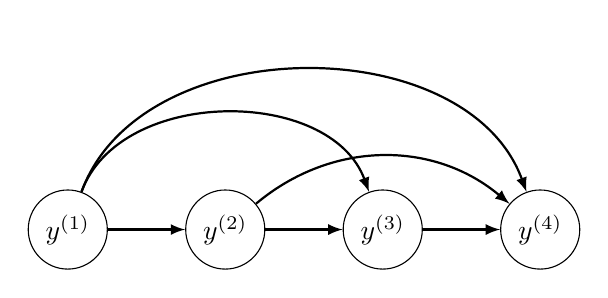
\begin{tikzpicture}[node distance=2cm,->,>=latex,auto,every edge/.append style={thick}]
	\node[state] (1) {$y^{(1)}$};
	\node[state] (2) [right of=1] {$y^{(2)}$};  
	\node[state] (3) [right of=2] {$y^{(3)}$};  
	\node[state] (4) [right of=3] {$y^{(4)}$};  
	
	\path(1) 
	edge[->] node{} (2)
	edge[bend left=70] node{} (3)
	edge[bend left=70] node{} (4);
	
	\path(2) 
	edge[->] node{} (3)
	edge[bend left=40] node{} (4);
	
	\path(3) edge[->] node{} (4);
	
	\end{tikzpicture}
\end{center}

If each value $y$ could take on the same fixed set of $k$ values, we would need to learn $k^4$ parameters to represent the joint distribution $P(\mathbb{Y})$. This clearly inefficient, since the number of parameters needed scales like $\mathcal{O}(k^\tau)$. If we relax the restriction that each $y^{(i)}$ must depend \textit{directly} on all past $y^{(j)}$, we can considerably reduce the number of parameters needed to compute the probability of some particular sequence. \\

\p We could include latent variables $h$ at each timestep that capture the dependencies, reminiscent of a classic RNN:

\begin{center}
	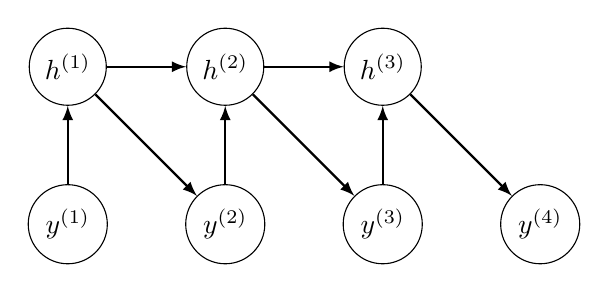
\begin{tikzpicture}[node distance=2cm,->,>=latex,auto,every edge/.append style={thick}]
	\node[state] (1) {$y^{(1)}$};
	\node[state] (2) [right of=1] {$y^{(2)}$};  
	\node[state] (3) [right of=2] {$y^{(3)}$};  
	\node[state] (4) [right of=3] {$y^{(4)}$};  
	
	\node[state] (h1) [above of=1]{$h^{(1)}$};
	\node[state] (h2) [above of=2]{$h^{(2)}$};
	\node[state] (h3) [above of=3]{$h^{(3)}$};
	
	\path(1) 	edge[->] node{} (h1);
	\path(2) 	edge[->] node{} (h2);
	\path(3) 	edge[->] node{} (h3);
	
	\path(h1) 	edge[->] node{} (h2)
	edge[->] node{} (2);
	
	\path(h2) 	edge[->] node{} (h3)
	edge[->] node{} (3);
	
	\path(h3) 	edge[->] node{} (4);
	\end{tikzpicture}
\end{center}
Since in the RNN case all factors $P(h^{(t)} \mid h^{(t-1)})$ are deterministic, we don't need any additional parameters to compute this probability\footnote{Don't forget that, in a neural net, a variable $y^{(t)}$ is represented by a \textit{layer}, which itself is composed of $k$ nodes, each associated with one of the $k$ unique values that $y^{(t)}$ could be.}, other than the single $m^2$ parameters needed to convert any $h^{(t)}$ to the next $h^{(t+1)}$ (which is shared across all transitions). Now, the number of parameters needed as a function of sequence length is constant, and as a function of $k$ is just $\mathcal{O}(k)$. \\

Finally, to view the RNN as a graphical model, we must describe how to sample from it, namely how to sample a sequence $\vec{y}$ from $P(\mathbb{Y})$, if parameterized by our graphical model above. In the general case where we don't know the value of $\tau$ for our sequence $\vec{y}$, one approach is to have a EOS symbol that, if found during sampling, means we should stop there. Also, in the typical case where we actually want to model $P(y \mid x)$ for input sequence $x$, we can reinterpret the parameters $\vec{\theta}$ of our graphical model as a function of $\vec{x}$ the input sequence. In other words, the graphical model interpretation becomes a function of $\vec{x}$, where $\vec{x}$ determines the exact values of the probabilities the graphical model takes on -- an ``instance'' of the graphical model.






\myspace
\p \blue{Bidirectional RNNs}. In many applications, it is desirable to output a prediction of $\vec{y}^{(t)}$ that may depend on \textit{the whole sequence}. For example, in speech recognition, the interpretation of words/sentences can also depend on what is \textit{about} to be said. Below is a typical bidirectional RNN, where the inputs $\vec{x}^(t)$ are fed both to a ``forward'' RNN ($\vec{h}$) and a ``backward'' RNN ($\vec{g}$). \marginnote{Notice how the output units $\vec{o}^{(t)}$ have the nice property of depending on both the past and future while being most sensitive to input values around time $t$.}[5em]

\myfig[0.3\textwidth]{BiRNN.PNG}

\myspace\myspace\Needspace{15\baselineskip}
\p \blue{Encoder-Decoder Seq2Seq Architectures (10.4)} Here we discuss how an RNN can be trained to map an input sequence to output sequence which is not necessarily the same length. (Not really much of a discussion...figure below says everything.)

\myfig{Seq2Seq.PNG}

\myspace\myspace\Needspace{15\baselineskip}
% --------------------------------------------
\subsub{Challenge of Long-Term Deps. (10.7)}
% --------------------------------------------

\myspace
\p Gradients propagated over many stages either vanish (usually) or explode. We saw how this could occur when we took parameter gradients earlier, and for weight matrices $\matr{W}$ further along from the loss node, the expression for $\matgrad{L}{W}$ contained multiplicative Jacobian factors. Consider the (linear activation) repeated function composition of an RNN's hidden state in \ref{10.36}. We can rewrite it as a power method (\ref{10.37}), and if $\matr{W}$ admits an eigendecomposition (remember $\matr{W}$ is necessarily square here), we can further simplify as seen in ~\ref{10.38}.\marginnote{\red{Q}: Explain interp. of mult. $\vec{h}$ by $\matr{Q}$ as opposed to the usual $\matr{Q}^T$ explained in the linear algebra review.}[2em]
\begin{align}
	\vec{h}^{(t)} &= \matr{W}^T \vec{h}^{(t-1)} \tlab{10.36} \\
	&= (\matr{W}^t)^T \vec{h}^{(0)} \tlab{10.37} \\
	&= \matr{Q}^T \matr{\Lambda}^t \matr{Q} \vec{h}^{(0)} \tlab{10.38}
\end{align}
\begin{quote}
	\textbf{Any component of $\vec{h}^{(0)}$ that isn't aligned with the largest eigenvector will eventually be discarded.}\footnote{Make sure to think about this from the right perspective. The largest value of $t = \tau$ in the RNNs we've seen would correspond with either (1) the largest output sequence or (2) the largest input sequence (if fixed-vector output). After we extract the output from a given forward pass, we reset the clock and either back-propagate errors (if training) or get ready to feed another sequence.}
\end{quote}
If, however, we have a non-recurrent network such that the state elements are repeatedly multiplied by different $w^{(t)}$ at each time step, the situation is different. Suppose the different $w^{(t)}$ are i.i.d. with mean 0 and variance $v$. The variance of the product is easily seen to be $\mathcal{O}(v^n)$\footnote{Quick sketch of (my) proof: \begin{align}
	 \Var{w^{(i)}} 
		 &= v 
			 = \E{(w^{(i)})^2} - \cancel{\E{w^{(i)}}^2} \\ 
	\Var{ \prod_t^n  w^{(t)}  } 
		&= \E{
			\left(
			\prod_t^n w^{(t)}
			\right)^2} 
		= \prod_t^n \E{  (    w^{ (t) }   )^2  } = v^n
	\end{align}}. \textit{To obtain some desired variance $v^*$ we may choose the individual weights with variance} $v = \sqrt[n]{v^*}$. 

\myspace\myspace\Needspace{15\baselineskip}
% --------------------------------------------
\subsub{LSTMs and Other Gated RNNs (10.10)}
% --------------------------------------------

\p While leaky units have connection weights that are either manually chosen constants or are trainable parameters, gated RNNs generalize this to connection weights that may change \textit{at each time step}. Furthermore, gated RNNs can learn to both accumulate and \textit{forget}, while leaky units are designed for just accumulation\footnote{Q: Isn't choosing to update with higher relative weight on the present the same as forgetting? A: Sort of. It's like ``soft forgetting'' and will inevitably erase more/less than desired (smeary). In this context, ``forget'' means to set the weight of a specific past cell to zero.}

\myspace
\p \blue{LSTM (10.10.1)}. The idea is we want self-loops to produce paths where the gradient can flow for long durations. The self-loop weights are \textbf{gated}, meaning they are controlled by another hidden unit, interpreted as being conditioned on \textit{context}. Listed below are the main components of the LSTM architecture.
\begin{compactitem}
	\item \textbf{Forget gate $f_i^{(t)} 
		= \sigma\left(b_i^f + \sum_j U_{i,j}^f x_j^{(t)} + \sum_j W_{i,j}^f h_j^{(t-1)}    \right)
		$}. \marginnote{The subscript, $i$, identifies the cell. The superscript, $t$, denotes the time.}
	
	\item \textbf{Internal state} $s_i^{(t)}
		= f_i^{(t)} \odot s_i^{(t-1)} + g_i^{(t)} \odot \sigma\left(b_i + \sum_j U_{i,j} x_j^{(t)} + \sum_j W_{i,j} h_j^{(t-1)}  \right)
		$. 
	
	\item \textbf{External input gate} $g_i^{(t)}
	= \sigma\left(b_i^g + \sum_j U_{i,j}^g x_j^{(t)} + \sum_j W_{i,j}^g h_j^{(t-1)}    \right)
	$.
	
	\item \textbf{Output gate} $q_i^{(t)}
	= \sigma\left(b_i^o + \sum_j U_{i,j}^o x_j^{(t)} + \sum_j W_{i,j}^o h_j^{(t-1)}    \right)
	$. 
\end{compactitem}
The final hidden state can then be computed via
\begin{align}
	h_i^{(t)} &= \tanh(s_i^{(t)}) \odot q_i^{(t)}
\end{align}










\lecture{Modern Practices}{Applications (Ch. 12)}{February 14}

\myspace

\subsub{Natural Language Processing (12.4)}

\marginnote{Begins on pg. 448}

\myspace
\p \blue{n-grams}. A \textbf{language model} defines a probability distribution over sequences of [discrete] tokens (words/characters/etc). Early models were based on the \textit{n-gram}: a [fixed-length] sequence of $n$ tokens. Such models define the conditional distribution for the $n$th token, given the $(n - 1)$ previous tokens: $$P(x_t \mid x_{t - (n - 1)}, \ldots, x_{t - 1})$$where $x_i$ denotes the token at step/index/position $i$ in the sequence. \\

\p To define distributions over longer sequences, we can just use Bayes rule over the shorter distributions, as usual. For example, say we want to find the [joint] distribution for some $\tau$-gram ($\tau > n$), and we have access to an $n$-gram model and a [perhaps different] model for the initial sequence $P(x_1, \ldots, x_{n - 1})$. We compute the $\tau$ distribution simply as follows:
\begin{align}
	P(x_1, \ldots, x_\tau) &= P(x_1, \ldots, x_{n - 1}) \prod_{t = n}^{\tau} 
		P(x_t \mid x_{t - 1}, \ldots, x_{t - (n - 2)}, x_{t - (n - 1)}) \tlab{12.5}
\end{align}
where it's important to see that each factor in the product is a distribution over a length-$n$ sequence. Since we need that initial factor, it is common to train both an $n$-gram model and an $n-1$-gram model simultaneously. \\

\p Let's do a specific example for a trigram (n = 3). 
\begin{compactitem}
	\item \textbf{Assumptions [for this trigram model example]}:
	\begin{compactitem}
		\item For any $n \ge 3$, $P(x_n \mid x_1, \ldots, x_{n - 1}) = P(x_n \mid x_{n - 2}, x_{n - 1})$. 
		
		\item When we get to computing the full joint distribution over some sequence of arbitrary length, we assume we have access to both $P_3$ and $P_2$, the joint distributions over all subsequences of length 3 and 2, respectively. 
	\end{compactitem}
	
	\item \textbf{Example sequence}: We want to know how to use a trigram model on the sequence ['THE', 'DOG', 'RAN', 'AWAY']. 
	
	\item \textbf{Derivation}: We can use the built-in model assumption to derive the following formula.
	\newcommand\fml[1]{\text{\footnotesize#1}}
	\begin{align}
	\begin{split}
		P(\fml{THE DOG RAN AWAY})
			&= P_3(\fml{AWAY} \mid \fml{THE DOG RAN})  ~ P_3(\fml{THE DOG RAN})\\
			&=  P_3(\fml{AWAY} \mid \fml{DOG RAN})  ~ P_3(\fml{THE DOG RAN})\\
			&= \frac{ P_3(\fml{DOG RAN AWAY}) }{ P_2(\fml{DOG RAN}) }  ~ P_3(\fml{THE DOG RAN})\\
			&= P_3(\fml{THE DOG RAN}) P_3(\fml{DOG RAN AWAY}) / P_2(\fml{DOG RAN})
	\end{split}\tlab{12.7}
	\end{align}
\end{compactitem}
\myspace
\p \blue{Limitations of n-gram}. The last example illustrates some potential problems one may encounter that arise [if using MLE] when the full joint we seek is nonzero, but (a) some $P_n$ factor is zero, or (b) $P_{n - 1}$ is zero\marginnote{Recall that, in MLE, the $P_n$ and $P_{n - 1}$ are usually approximated via counting occurrences in the training set}[-2em]. Some methods of dealing with this are as follows.
\begin{compactitem}
	\item \textbf{Smoothing}: shifting probability mass from the observed tuples to unobserved ones that are similar.
	\item \textbf{Back-off methods}: look up the lower-order (lower values of $n$) $n$-grams if the frequency of the context $x_{t - 1}, \ldots, x_{t - (n - 1)}$ is too small to use the higher-order model.
\end{compactitem}
In addition, $n$-gram models are vulnerable to the curse of dimensionality, since most $n$-grams won't occur in the training set\footnote{For a given vocabulary, which usually has much more than $n$ possible words, consider how many possible sequences of length $n$.}, even for modest $n$.


% =========================================
\subsub{Neural Language Models (12.4.2)}
% =========================================

\p Designed to overcome curse of dimensionality by using a distributed representation of words. Recognize that any model trained on sentences of length $n$ and then told to generalize to new sentences [also of length $n$] must deal with a space\footnote{Ok I tried re-wording that from the book's confusing wording but that was also a bit confusing. Let me break it down. Say you train on a thousand sentences each of length 5. For a given vocabulary of size VOCAB\_SIZE, the number of possible sequences of length 5 is $(\text{VOCAB\_SIZE})^5$, which can be quite a lot more than a thousand (not to mention the possibility of duplicate training examples). To the naive model, all points in this high-dimensional space are basically the same. A neural language model, however, tries to arrange the space of possibilities in a meaningful way, so that an unforeseen sample at test time can be said "similar" as some previously seen training example. It does this by \textit{embedding} words/sentences in a lower-dimensional feature space.} of possible sentences that is exponential in $n$. Such word representations (i.e. viewing words as existing in some high-dimensional space) are often called \textbf{word embeddings}. The idea is to map the words (or sentences) from the raw high-dimensional [vocab sized] space to a smaller feature space, where similar words are closer to one another. Using distributed representations may also be used with graphical models (think Bayes' nets) in the form multiple \textit{latent variables}. 










% ==================================================================================
% DEEP LEARNING RESEARCH
% ==================================================================================
\mysection{Deep Learning Research}\label{Deep Learning Research}

\lecture{Deep Learning Research}{Linear Factor Models (Ch. 13)}{January 12}

\myspace
\p \blue{Overview}. Much research is in building a \textit{probabilistic model}\footnote{Whereas, before, we've been building \textit{functions} of the input (deterministic).} of the input, $p_{model}(x)$. Why? Because then we can perform \textit{inference} to predict stuff about our environment given any of the other variables. We call the other variables \textbf{latent variables}, $h$, with
\begin{align}
	p_{model}(x) &= \sum_h \Pr(h)\Pr(x \mid h) = \mathbb{E}_h\left[ p_{model}(x \mid h)\right]
\end{align}
So what? Well, the latent variables provide another means of \textit{data representation}, which can be useful. \textbf{Linear factor models} (LFM) are some of the simplest probabilistic models with latent variables.
\begin{quote}
	A linear factor model is defined by the use of a stochastic linear decoder function that generates $\vec{x}$ by adding noise to a linear transformation of $\vec{h}$. 
\end{quote}
Note that $\vec{h}$ is a \textit{vector} of arbitrary size, where we assume $p(\vec{h})$ is a \purple{factorial distribution}: $p(\vec{h}) = \prod_i p(h_i)$. This roughly means we assume the elements of $\vec{h}$ are mutually independent\footnote{Note that, technically, this assumption isn't strictly the definition of mutual independence, which requires that every \textit{subset} (i.e. not just the full set) of $\{h_i \in \vec{h}\}$ follow this factorial property.}. The LFM describes the data-generation process as follows:
\begin{compactenum}
	\item Sample the explanatory factors: $\vec{h} \sim p(\vec{h})$.
	\item Sample the real-valued observable variables given the factors:
	
	\graybox{
		\vec{x} = \matr{W} \vec{h} + \vec{b} + \textrm{noise}
		}
\end{compactenum}

\myspace
\p \blue{Probabilistic PCA and Factor Analysis}.
\begin{compactitem}
	\item \textbf{Factor analysis}: 
	\begin{align}
		\vec{h} &\sim \mathcal{N}(\vec{h}; \vec{0}, \matr{I}) \\
		\text{noise} &\sim \mathcal{N}(\vec{0}, \vec{\psi}\equiv\text{diag}(\vec{\sigma^2})) \\
		\vec{x} &\sim \mathcal{N}(\vec{x};~ \vec{b}, \matr{W}\matr{W}^T + \vec{\psi})
	\end{align}
	where the last relation can be shown by recalling that a linear combination of Gaussian variables is itself Gaussian, and showing that $\mathbb{E}_h\left[\vec{x}\right] = \vec{b}$, and $\text{Cov}(\vec{x}) = \matr{W}\matr{W}^T + \vec{\psi}$. \\
	
	\p It is worth emphasizing the interpretation of $\vec{\psi}$ as the matrix of \green{conditional variances} $\sigma_i^2$. \textit{Huh?} Let's take a step back. The fact that we were able to separate the distributions in the above relations for $\vec{h}$ and $\text{noise}$ is from a built-in \underline{assumption} that $\Pr(x_i | \vec{h}, x_{j \ne i}) = \Pr(x_i | \vec{h})$\footnote{Due to $<$\textsc{math}$>$, this introduces a constraint that knowing the value of some element $x_j$ doesn't alter the probability $\Pr(x_i = W_i \cdot h + b_i + \text{noise})$. Given how we've defined the variable $\vec{h}$, this means that knowing $\text{noise}_j$ provides no clues about $\text{noise}_i$. Mathematically, the noise must have a diagonal covariance matrix.}. \\
	
	\redbox[The Big Idea]{
		The latent variable $\vec{h}$ is a big deal because it \textbf{captures the dependencies} between the elements of $\vec{x}$. \textit{How do I know?} Because of our assumption that the $x_i$ are conditionally independent given $\vec{h}$. If, once we specify $\vec{h}$, all the elements of $\vec{x}$ become independent, then any information about their interrelationship is hiding somewhere in $\vec{h}$.
	}
	\vspace{0.3em}
	Detailed walkthrough of Factor Analysis (a.k.a me slowly reviewing, months after taking this note):
	{\small
	\begin{compactitem}
		\item \textbf{Goal}. Analyze and understand the motivations behind how Factor Analysis defines the data-generation process under the framework of LFMs (defined in steps 1 and 2 earlier). Assume $\vec{h}$ has dimension $n$. 
		\item \textbf{Prior}. Defines $p(\vec{h}) := \mathcal{N}(\vec{h}; \vec{0}, \matr{I})$, the unit-variance Gaussian. Explicitly,
			$$
				p(\vec{h}) := \frac{1}{(2\pi)^{n/2}} e^{-\frac{1}{2} \sum_i^n h_i^2}
			$$
		\item \textbf{Noise}. Assumed to be drawn from a Gaussian with diagonal covariance matrix $\matr{\psi} := \diag{\vec{\sigma}^2}$. Explicitly,
		$$
			p(\text{noise} = \vec{a}) := \frac{1}{ (2\pi)^{n / 2} \prod_i^n \sigma_i } e^{-\frac{1}{2} \sum_i^n a_i^2 / \sigma_i^2}
		$$
		
		\item \textbf{Deriving distribution of $\vec{x}$}. We use the fact that any linear combination of Gaussians is itself Gaussian. Thus, deriving $p(\vec{x})$ is reduced to computing it's mean and covariance matrix.
		\begin{align}
			\vec[x]{\mu} &= \E[\vec{h}]{\matr{W} \vec{h} + \vec{b}} \\
			&= \int p(\vec{h}) (\matr{W} \vec{h} + \vec{b}) \mathrm{d}\vec{h} \\
			&= \vec{b} + \int \frac{1}{(2\pi)^{n/2}} e^{-\frac{1}{2} \sum_i^n h_i^2} \matr{W} \vec{h} \mathrm{d}\vec{h} \\
			&= \vec{b} \\
			\text{Cov}(\vec{x}) &= \E{(\vec{x} - \E{\vec{x}}) (\vec{x} - \E{\vec{x}})^T} \\
			&= \E{(\matr{W}\vec{h} + \text{noise})(\vec{h}^T \matr{W}^T + \text{noise}^T)} \\
			&= \E{(\matr{W}\vec{h}\vec{h}^T\matr{W}^T)} + \matr{\psi} \\
			&= \matr{W}\matr{W}^T + \matr{\psi}
		\end{align}
		where we compute the expectation of $\vec{x}$ over $\vec{h}$ because $\vec{x}$ is defined as a function of $\vec{h}$, and noise is always expectation zero.
		\item \textbf{Thoughts}. Not really seeing why this is useful/noteworthy. Feels very contrived (many assumptions) and restrictive -- it only applies if the dependencies between each $x_i$ can be modeled with a random variable $\vec{h}$ sampled from a unit variance Gaussian.
	\end{compactitem}}
	
	
	
	\vspace{0.3em}
	\item \textbf{Probabilistic PCA}: Just factor analysis with $\vec{\psi} = \sigma^2 \matr{I}$. So zero-mean spherical Gaussian noise. It becomes regular PCA as $\sigma \rightarrow 0$. Here we can use an iterative EM algorithm for estimating the parameters $\matr{W}$. 
\end{compactitem}

%
% AUTOENCODERS
% 
\lecture{Deep Learning Research}{Autoencoders (Ch. 14)}{May 07}

\p \blue{Introduction}. An autoencoder learns to copy its input to its output, via an encoder function $\vec{h} = f(\vec{x})$ and a decoder function $\vec{r} = g(\vec{h})$\marginnote{$\vec{r}$ for ``reconstruction''}. Modern autoencoders generalize this to allow for stochastic mappings $p_{encoder}(\vec{h} \mid \vec{x})$ and $p_{decoder}(\vec{x} \mid \vec{h})$.

\myspace
\p \blue{Undercomplete Autoencoders}. Constrain dimension of $\vec{h}$ to be smaller than that of $\vec{x}$. The learning process minimizes some $L(\vec{x}, g(f(\vec{x})))$, where the loss function could be e.g. mean squared error. Be careful not to have too many learnable parameters in the functions $g$ and $f$ (thus increasing model capacity), since that defeats the purpose of using an undercomplete autoencoder in the first place.

\myspace
\p \blue{Regularized Autoencoders}. We can remove the undercomplete constraint/necessity by modifying our loss function. For example, a \green{sparse autoencoder} one that adds a penalty $\Omega(\vec{h})$ to the loss function that encourages the \textit{activations on} (not connections to/from) the hidden layer to be sparse. One way to achieve \textit{actual zeros} in $\vec{h}$ is to use rectified linear units for the activations.


%
% AUTOENCODERS
% 
\lecture{Deep Learning Research}{Representation Learning (Ch. 15)}{May 07}

\myspace
\p \blue{Greedy Layer-Wise Unsupervised Pretraining}. Given:
\begin{compactitem}[-]
	\item Unsupervised learning algorithm $\mathcal{L}$ which accepts as input a training set of examples $\matr{X}$, and outputs an encoder/feature function $f$. 
	\item $f^{(i)}(\matr{\tilde{X}})$ denotes the output of the $i$th layer of $f$, given as \textit{immediate input} the (possibly transformed) set of examples $\matr{\tilde{X}}$.
	\item Let $m$ denote the number of layers (``stages'') in the encoder function (note that each layer/stage here \textit{must} use a representation learning algorithm for its $\mathcal{L}$ e.g. an RBM, autoencoder, sparse coding model, etc.)
\end{compactitem}
The procedure is as follows:
\begin{compactenum}
	\item Initialize.
	\begin{align}
		f(\cdot) &\leftarrow I(\cdot) \\
		\tilde{\matr{X}} &= \matr{X}
	\end{align}
	
	\item For each layer (stage) $i$ in $\text{range}(m)$, do:
	\begin{align}
		f^{(k)} &= \mathcal{L}(\tilde{\matr{X}}) \\
		f(\cdot) &\leftarrow  f^{(k)}\left(f\left(\cdot\right)\right) \\
		\tilde{\matr{X}} &\leftarrow f^{(k)}(\tilde{\matr{X}})
	\end{align}
	In English: just apply the regular learning/training process for each layer/stage \textbf{sequentially and individually}\footnote{In other words, you proceed one layer at a time \textit{in order}. You don't touch layer $i$ until the weights in layer $i - 1$ have been learned.}.
\end{compactenum}
When this is complete, we can run \green{fine-tuning}: train all layers together (including any later layers that could not be pretrained) with a supervised learning algorithm. Note that we do indeed allow the pretrained encoding stages to be optimized here (i.e. not fixed).

% 
% PROBABILISTIC MODELS
% 
\lecture{Deep Learning Research}{Structured Probabilistic Models for DL (Ch. 16)}{October 01, 2017}

\p \blue{Motivation}. In addition to classification, we can ask probabilistic models to perform other tasks such as density estimation ($\vec{x} \rightarrow p(\vec{x})$), denoising, missing value imputation, or sampling. What these [other] tasks have in common is they require a \textit{complete understanding of the input}. Let's start with the most naive approach of modeling $p(\vec{x})$, where $\vec{x}$ contains $n$ elements, each of which can take on $k$ distinct values: we store a lookup table of all possible $\vec{x}$ and the corresponding probability value $p(\vec{x})$. This requires $k^n$ parameters\footnote{Consider the common NLP case where our vector $\vec{x}$ contains $n$ word tokens, each of which can take on any symbol in our vocabulary of size $v$. If we assign $n=100$ and $v=100,000$, which are relatively common values for this case, this amounts to $(1e5)^{1e2} = 10^{500}$ parameters.}. Instead, we use graphs to describe model structure (direct/indirect interactions) to drastically reduce the number of parameters.

\myspace
\p \blue{Directed Models}. Also called \green{belief networks} or \green{Bayesian networks}. Formally, a directed graphical model defined on a set of variables $\{\vec{x}\}$ is defined by a DAG, $\mathcal{G}$, whose vertices are the random variables in the model, and a set of \textbf{local conditional probability distributions}, $p(x_i \mid Pa_{\mathcal{G}}(x_i))$, where $Pa_{\mathcal{G}}(x_i)$ gives the parents of $x_i$ in $\mathcal{G}$. The probability distribution over $\vec{x}$ is given by
\graybox{
	p(\vec{x}) = \prod_i p(x_i \mid Pa_{\mathcal{G}}(x_i))
	}
	
\myspace
\p \blue{Undirected Graphical Models}. Also called \green{Markov Random Fields (MRFs)} or \green{Markov Networks}. Appropriate for situations where interactions do not have a well-defined direction. Each \green{clique} $\mathcal{C}$ (any set of nodes that are all [maximally] connected) in $\mathcal{G}$ is associated with a factor $\phi(\mathcal{C})$. The factor $\phi(\mathcal{C})$, also called a \green{clique potential}, is just a function (not necessarily a probability) that outputs a number when given a possible set of values over the nodes in $\mathcal{C}$. The output number measures the affinity of the variables in that clique for being in the states specified by the inputs\marginnote{Clique potentials are constrained to be nonnegative.}[-2em]. The set of all factors in $\mathcal{G}$ defines an \textbf{unnormalized probability distribution}:
\graybox{
	\widetilde{p}(\vec{x}) = \prod_{\mathcal{C} \in \mathcal{G}} \phi(\mathcal{C})
	}

\myspace
\p \blue{The Partition Function}. To obtain a valid probability distribution, we must normalize the probability distribution:
\begin{align}
	p(\vec{x}) &= \frac{1}{Z} \widetilde{p}(\vec{x}) \\
	Z &= \int \widetilde{p}(\vec{x}) \mathrm{d}\vec{x}
\end{align}
where the normalizing function $Z = Z(\{\phi\})$ is known as the \green{partition function} (physicz sh0ut0uT). It is typically intractable to compute, so we resort to approximations. Note that $Z$ isn't even guaranteed to exist -- it's only for those definitions of the clique potentials that cause the integral over $\widetilde{p}(\vec{x})$ to converge/be defined.

\myspace
\p \blue{Energy-Based Models} (EBMs). A convenient way to enforce $\forall \vec{x}, ~ \widetilde{p}(\vec{x}) > 0$ is to use EBMs, where
\begin{align}
	\widetilde{p}(\vec{x}) \triangleq \exp\left( -E(\vec{x}) \right)
\end{align}
and $E(\vec{x})$ is known as the \green{energy function}\footnote{Physics throwback: this mirrors the Boltzmann factor, $\exp(-\varepsilon/\tau)$, which is proportional to the probability of the system being in quantum energy state $\varepsilon$.}. Many algorithms need to compute not $p_{model}(\vec{x})$ but only $\log\widetilde{p}_{model}(\vec{x})$ (unnormalized log probabilities - logits!). For EBMs with latent variables $\vec{h}$, such algorithms are phrased in terms of the \green{free energy}:
\begin{align}
	\mathcal{F}(\vec{x} = x) &= -\log \sum_{h} \exp\left( - E(\vec{x}=x, ~ \vec{h} = h ) \right)
\end{align}
where we sum over all possible assignments of the latent variables.


\myspace
\p \blue{Separation and D-Separation}. We want to know which subsets of variables are conditionally independent from each other, given the values of other subsets of variables.  A set of variables $\mathbb{A}$ is \green{separated} (if undirected model)/\green{d-separated} (if directed model) from another set of variables $\mathbb{B}$ given a third set of variables $\mathbb{S}$ if the graph structure implies that $\mathbb{A}$ is independent from $\mathbb{B}$ given $\mathbb{S}$. 

\begin{compactitem}
	\item \green{Separation}. For \textit{undirected} models. If variables $a$ and $b$ are connected by a path involving only \underline{unobserved} variables (an \green{active} path), then $a$ and $b$ are \textit{not} separated. Otherwise, they are separated. Any paths containing at least one observed variable are called \green{inactive}.

	\item \green{D-Separation}\footnote{The D stands for dependence.}. For \textit{directed} models. Although there are rules that help determine whether a path between $a$ and $b$ is d-separated, it is simplest to just determine whether $a$ is independent from $b$ given any observed variables along the path.
\end{compactitem}


% ------------------------------------------------
\myspace\Needspace{18\baselineskip}
\subsub{Sampling from Graphical Models}
\myspace
% ------------------------------------------------

\p For directed graphical models, we can do \green{ancestral sampling} to produce a sample $\vec{x}$ from the joint distribution represented by the model. Just sort the variables $x_i$ into a topological ordering such that $\forall i,j: j > i \iff x_i \in Pa_{\mathcal{G}}(x_j)$. To produce the sample, just sequentially sample from the beginning, $x_1 \sim P(x_1)$, $x_2 \sim P(x_2 \mid Pa_{\mathcal{G}}(x_1) )$, etc.\\

\p For undirected graphical models, one simple approach is \green{Gibbs sampling}. Essentially, this involves drawing a conditioned sample from $x_i \sim p(x_i \mid \text{neighbors}(x_i))$ for each $x_i$. This process is repeated many times, where each subsequent pass uses the previously sampled values in $\text{neighbors}(x_i)$ to obtain an asymptotically converging [to the correct distribution] estimate for a sample from $p(\vec{x})$.

% ------------------------------------------------
\myspace\Needspace{18\baselineskip}
\subsub{Inference and Approximate Inference}
\myspace
% ------------------------------------------------

\p One of the main tasks with graphical models is predicting the values of some subset of variables given another subset: inference. Although the graph structures we've discussed allow us to represent complicated, high-dimensional distributions with a reasonable number of parameters, the graphs used for deep learning are usually not restrictive enough to allow efficient inference. \green{Approximate inference} for deep learning usually refers to variational inference, in which we approximate the distribution $p(\vec{h} \mid \vec{v})$ by seeking an approximate distribution $q(\vec{h} \mid \vec{v})$ that is as close to the true one as possible. 

\myspace
\p \blue{Example: Restricted Boltzmann Machine}. The quintessential example of how graphical models are used for deep learning. The canonical RBM is an energy-based model with \textbf{binary} visible and hidden units. Its energy function is
\graybox{
	E(\vec{v}, \vec{h}) &= -\vec{b}^T\vec{v} - \vec{c}^T\vec{h} - \vec{v}^T\matr{W}\vec{h}
	}
where $\vec{b}$, $\vec{c}$, and $\matr{W}$ are unconstrained, real-valued, learnable parameters. One could interpret the values of the bias parameters as the affinities for the associated variable being its given value, and the value $\matr[i,j]{W}$ as the affinity of $v_i$ being its value and $h_j$ being its value at the same time\footnote{More concretely, remember that $\vec{v}$ is a one-hot vector representing some state that can assume len($\vec{v}$) unique values, and similarly for $\vec{h}$. Then $\matr[i,j]{W}$ gives the affinity for the state associated with $v$ being its $i$th value \textit{and} the state associated with $h$ being its $j$th value.}. \\

The restrictions on the RBM structure, namely the fact that there are no intra-layer connections, yields nice properties. Since $\widetilde p(\vec{h},\vec{v})$ can be factored into clique potentials, we can say that:
\begin{align}
	p(\vec{h} \mid \vec{v}) &= \prod_i p(h_i \mid \vec{v}) \\
	p(\vec{v} \mid \vec{h}) &= \prod_i p(v_i \mid \vec{h})
\end{align}
Also, due to the restriction of binary variables, each of the conditionals is easy to compute, and can be quickly derived as
\begin{align}
	p(h_i = 1 \mid \vec{v}) &= \sigma\left( c_i + \vec{v}^T\matr[:,i]{W} \right)
\end{align}
allowing for efficient block Gibbs sampling. 



%
% MONTE CARLO METHODS
% 
\lecture{Deep Learning Research}{Monte Carlo Methods (Ch. 17)}{May 09}

\p \blue{Monte Carlo Sampling (Basics)}. We can approximate the value of a (usually prohibitively large) sum/integral by viewing it as an \textit{expectation} under some distribution. We can then approximate its value by taking samples from the corresponding probability distribution and taking an empirical average. Mathematically, the basic idea is show below:
\graybox{
	s = \int p(\vec{x}) f(\vec{x}) \mathrm{d}\vec{x} = \E[p]{f(\rvec{x})}
	\quad\rightarrow\quad
	\hat{s}_n = \frac{1}{n} \sum_{i = 1,~\rvec{x}^{(i)} \sim p}^{n} f(\vec{x}^{(i)})
}
As we've seen before, the empirical average is an unbiased\footnote{
	Recall that expectations on such an average are still taken over the underlying (assumed) probability distribution:
	\begin{align}
		\E[p]{\hat{s}_n} &= \frac{1}{n} \sum_{i = 1}^{n} \E[p]{f(\vec{x}^{(i)})} \\
		&= \frac{1}{n} \sum_{i = 1}^{n} s \\
		&= s
	\end{align}
	You should think of the expectation $\E[p]{f(\vec{x}^{(i)})}$ as the expected value of the \textit{random sample} from the underlying distribution, which of course is $s$, because we defined it that way. 
	} estimator. Furthermore, the central limit theorem tells us that the distribution of $\hat{s}_n$ converges to a normal distribution with mean $s$ and variance $\Var{f(\vec{x})}/n$. 
	
\myspace
\p \blue{Importance Sampling}. What if it's not feasible for us to sample from $p$? We can approach this a couple ways, both of which will exploit the following identity:
\begin{align}
	p(\vec{x}) f(\vec{x}) = q(\vec{x}) \frac{p(\vec{x}) f(\vec{x})}{q(\vec{x})}
\end{align}
\begin{itemize}
	\item \textbf{Optimal importance sampling}. We can use the aforementioned identity/decomposition to find the \green{optimal $q*$} -- optimal in terms of number of samples required to achieve a given level of accuracy. First, we rewrite our estimator $\hat{s}_p$ (they now use subscript to denote the sampling distribution) as $\hat{s}_q$:
	\begin{align}
		\hat{s}_q &=  \frac{1}{n} \sum_{i = 1,~\rvec{x}^{(i)} \sim q}^{n} \frac{p(\vec{x}^{(i)}) f(\vec{x}^{(i)})}{q(\vec{x}^{(i)})}
	\end{align}
	At first glance, it feels a little wonky, but recognize that we are \textit{sampling from q instead of p} (i.e. if this were an integral, it would be over $q(\vec{x})\mathrm{d}\vec{x}$). The catch is that, now, the variance can be greatly sensitive to the choice of $q$:
	\begin{align}
		\Var{\hat{s}_q} &= \Var{\frac{p(\vec{x}) f(\vec{x})}{q(\vec{x})}} / n
	\end{align}
	with the optimal (minimum) value of $q$ at:
	\graybox{
		q* &= \frac{p(\vec{x})\mid f(\vec{x}) \mid}{Z}
		}
		
	\item \textbf{Biased importance sampling}. Computing the optimal value of $q$ can be as challenging/infeasible as sampling from $p$. Biased sampling does not require us to find a normalization constant for $p$ or $q$. Instead, we compute:
	\begin{align}
		\hat{s}_{BIS} &= \dfrac{
			\sum_{i = 1}^{n} \frac{\tilde p(\vec{x}^{(i)})}{\tilde q(\vec{x}^{(i)})}  f(\vec{x}^{(i)})
			}{
			\sum_{i = 1}^{n} \frac{\tilde p(\vec{x}^{(i)})}{\tilde q(\vec{x}^{(i)})}  
			}
	\end{align}
	where $\tilde p$ and $\tilde q$ are the unnormalized forms of $p$ and $q$, and the $\vec{x}^{(i)}$ samples are still drawn from [the original/unknown] $q$. $\E{\hat s_{BIS}} \ne s$ except asymptotically when $n \rightarrow \infty$. 
\end{itemize}







%
% Confronting the Partition Function
% 
\lecture{Deep Learning Research}{Confronting the Partition Function (Ch. 18)}{August 30, 2018}



\p \blue{Noise Contrastive Estimation} (NCE) (18.6). We now estimate
\begin{align}
	\log p_{model}(\vec x)
		&= \log \tilde{p}_{model}(\vec x; \vec\theta) + c
\end{align}
and explicitly learn an approximation, $c$, for $-\log Z(\vec\theta)$. Obviously MLE would just try jacking up $c$ to maximize this, so we adopt a surrogate supervised training problem: binary classification that a given sample $\vec x$ belongs to the (true) data distribution $p_{data}$ or to the noise distribution $p_{noise}$. We introduce binary variable $y$ to indicate whether the sample is in the true data distribution ($y{=}1$) or the noise distribution ($y{=}0$). Our surrogate model is thus defined by
\begin{align}
	p_{joint}(y{=}1) &= \onehalf \\
	p_{joint}(\vec x \mid y{=}1) &= p_{model}(\vec x) \\
	p_{joint}(\vec x \mid y{=}0) &= p_{noise}(\vec x) 
\end{align}
We can now use MLE on the optimization problem,
\graybox{
	\vec\theta , c 
		&= \argmax_{\vec\theta , c} \E[\vec x, y \sim p_{train}]{\log p_{joint}(y \mid \vec x)} \\
	p_{joint}(y{=}1 \mid \vec x)
		&= \frac{  p_{model}(\vec x) }{  p_{model}(\vec x) + p_{noise}(\vec x) } \\
		&= \inv{  1 + p_{noise}(\vec x) / p_{model}(\vec x)  } \\
		&= \sigma\left(  
			\log p_{model}\left( \vec x \right) -
			\log p_{noise}\left( \vec x \right)
		\right)
}

































%
% APPROXIMATE INFERENCE
% 
\lecture{Deep Learning Research}{Approximate Inference (Ch. 19)}{Nov 15, 2017}

% log(p(v; theta))
\newcommand\lpv{\log p(\vec{v}; \vec{\theta})}
\newcommand\elbo{\mathcal{L}(\vec v, \vec{\theta}, q)}
\newcommand\Dkl[2]{D_{KL}\left( #1 ~||~ #2 \right)}

\p \blue{Overview}. Most graphical models with multiple layers of hidden variables have intractable posterior distributions. This is typically because the partition function scales exponentially with the number of units and/or due to marginalizing out latent variables. Many approximate inference approaches make use of the observation that exact inference can be described as an optimization problem. \\ 

Assume we have a probabilistic model consisting of observed variables $\vec{v}$ and latent variables $\vec{h}$. We want to compute $\log p(\vec v;\vec{\theta})$, but it's too costly to marginalize out $\vec{h}$. Instead, we compute a lower bound $\mathcal{L}(\vec v, \vec{\theta}, q)$ -- often called the \green{evidence lower bound} (ELBO) or negative \green{variational free energy} -- on $\log p(\vec v; \vec{\theta})$\footnote{Recall that $D_{KL}(P || Q) = \E[x \sim P(x)]{\log \frac{P(x)}{Q(x)} }$}:\marginnote{$q$ is an arbitrary probability distribution over $\vec{h}$. Note that the book will write $q$ when they really mean $q(\vec h \mid \vec v)$.}[2em]
\graybox{
	\elbo &= \lpv - \Dkl{ q(\vec{h} \mid \vec{v}) }{p(\vec{h} \mid \vec{v}; \vec{\theta})} \\
	&= - \E[\vec{h} \sim q(\vec h \mid \vec v)]{\log p(\vec h, \vec v)} + H(q(\vec h \mid \vec v))
}
where the second form is the more canonical definition\footnote{This can be derived easily from the first form. Hint: $$
	\log \frac{q(\vec h \mid \vec v)}{ p(\vec h \mid \vec v)} = 
	\log \frac{q(\vec h \mid \vec v)}{ p(\vec h, \vec v; \vec{\theta}) / p(\vec v; \vec{\theta})} 
$$}. Note that $\elbo$ is a lower-bound on $\lpv$ by definition, since 
$$\lpv - \elbo = D_{KL}\left(q(\vec{h} \mid \vec{v}) ||
p(\vec{h} \mid \vec{v}; \vec{\theta}) \right) \ge 0
$$
With equality (to zero) iff $q$ is the same distribution as $p(\vec h \mid \vec v)$. In other words, $\mathcal L$ can be viewed as a function parameterized by $q$ that's maximized when $q$ is $p(\vec h \mid \vec v)$, and with maximal value $\log p(\vec v)$. Therefore, we can cast the \textit{inference} problem of computing the (log) probability of the observed data  $\log p(\vec v)$ into an \textit{optimization} problem of maximizing $\mathcal L$. Exact inference can be done by searching over a family of functions that contains $p(\vec h \mid \vec v)$. 

\myspace
\p \blue{Expectation Maximization} (19.2). Technically not an approach to approximate inference, but rather an approach to learning with an approximate posterior. Popular for training models with latent variables. The EM algorithm consists of alternating between the followi[p]ng 2 steps until convergence:
\begin{compactenum}
	\item \textbf{E-step}. For each training example $\vec{v}^{(i)}$ (in current batch or full set), set
	\begin{align}
		q(\vec{h} \mid \vec{v}^{(i)}  )
			&= p(\vec{h} \mid \vec{v}^{(i)}; \vec{\theta}^{(0)})
	\end{align}
	where $\vec{\theta}^{(0)}$ denotes the current parameter values of the model at the beginning of the E-step. This can also be interpreted as maximizing $\mathcal L$ w.r.t. $q$. 
	
	\item \textbf{M-step}. Update the parameters $\vec{\theta}$ by completely or partially finding
	\begin{align}
		\argmax_{\vec{\theta}} \sum_i \mathcal{L}\left(\vec{v}^{(i)}, \vec{\theta}, q(\vec{h} \mid \vec{v}^{(i)}; \vec{\theta}^{(0)} ) \right)
	\end{align} 
\end{compactenum}













%
% APPROXIMATE INFERENCE
% 
\lecture{Deep Learning Research}{Deep Generative Models (Ch. 20)}{July 28, 2018}


\p \blue{Boltzmann Machines} (20.1). An energy-based model over a $d$-dimensional binary random vector $\rvec{x} \in \{0, 1\}^d$. The energy function is simply $E(\vec{x}) = -\vec{x}^T \matr U \vec x - \vec{b}^T \vec x$, i.e. parameters between all pairs of $x_i, x_j$, and bias parameters for each $x_i$\footnote{Authors are being lazy because it's assumed the reader is familiar (which is fair, I guess). i.e. they aren't mentioning that this formula implies that $\matr U$ is either lower or upper triangular, and the diagonal is zero.}. In settings where our data consists of samples of fully observed $\vec x$, this is clearly limited to very simple cases, since e.g. the probability of some $x_i$ being on is given by logistic regression from the values of the other units. 

\begin{example}[Proof: prob of \(x_i\) being on is logistic regression on other units]
	\tiny
	It's important to be as specific as possible here, since the task stated as-is is ambiguous. We want to prove that the probability of some fully observed state $\vec x$ that has its $i$th element clamped to $1$, which I'll denote as $p_{i=on}(\vec x)$, is logistic regression over the other units.\\
	
	To prove this, it's easier to use the conventional definition where $\matr U$ is symmetric with zero diagonal, and we write $E(\vec x)$ as
	\begin{align}
		E(\vec x)
			&= - \sum_{i=1}^{d} \sum_{j=i+1}^{d} x_i U_{i,j} x_j - \sum_{i=1}^{d} b_i x_i
	\end{align}
	where the difference is that we explicitly only sum over the upper triangle of $\matr U$. \\
	
	Intuitively, since $p(\{ \vec x \}_{j \ne i}) = p_{i=on}(\vec x) + p_{i=off}(\vec x)$, our final formula for $p_{i=on}$ should only contain terms involving the parameters that interact with $x_i$, and only for those cases where $x_i=1$. This motivates exploring the formula for $\Delta E_i (\vec x) \triangleq E_{i=off} - E_{i=on}$ where I've dropped the explicit notation on $\vec x$ for simplicity/space. Before jumping in to deriving this, step back and realize that $\Delta E_i$ will only contain summation terms where either the row or column index of $\matr U$ is $i$, and only for terms with bias element $b_i$. Since our summation is over the upper triangle of $\matr U$, this means terms along the slices $U_{i, i+1:d}$ and $U_{1:i-1, i}$. Now there is no derivation needed and we can simply write
	\begin{align}
		\Delta E_i 
			&= \sum_{k = i + 1}^{d} U_{i, k} x_k + \sum_{k = 1}^{i-1} x_k U_{k, i} + b_i 
	\end{align}
	
	The goal is to use this to get a logistic-regression-like formula for $p_{i=on}$, so we should now think about the relationship between any given $p(\vec x)$ and the associated $E(\vec x)$. The critical observation is that $E(\vec x) = -\ln p(\vec x) - \ln Z$, which therefore means
	\begin{align}
		\Delta E_i
			&= \ln p_{i=on}(\vec x) - \ln p_{i=off}(\vec x)
			= - \ln\left( \frac{ 1 - p_{i=on}(\vec x)  }{p_{i=on}(\vec x)}  \right) \\
		\exp(- \Delta E_i)
			&=  \frac{ 1 - p_{i=on}(\vec x)  }{p_{i=on}(\vec x)} =  \frac{ 1 }{p_{i=on}(\vec x)} - 1 \\
		\therefore p_{i=on}(\vec x)
			&= \frac{ 1 }{ 1 +  \exp(- \Delta E_i) }
	\end{align}
	Since $\Delta E_i$ is a linear function of all other units, we have proven that $p_{i=on}(\vec x)$ for some state $\vec x$ reduces to logistic regression over the other units. 
\end{example}

\myspace
\p \blue{Restricted Boltzmann Machines} (20.2). A BM with variables partitioned into two sets: hidden and observed. The graphical model is bipartite over the hidden and observed nodes, as I've drawn in the example below. 
\begin{center}
	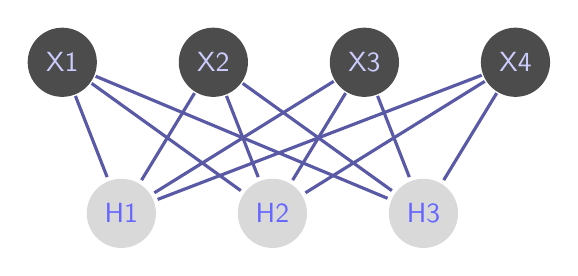
\begin{tikzpicture}[font=\sffamily,node distance=1.cm,->,>=latex,auto,line width=0.4mm]
	
	\tikzset{node st/.style={state, draw=none,
			fill=gray!30!white,
			text=blue!60!white}}
	\tikzset{node obs/.style={state, draw=none,
			fill=gray!60!black,
			text=blue!20!white}}
	
	\node[node obs] (X1) {X1};
	\node[node obs, right=of X1] (X2) {X2};
	\node[node obs, right=of X2] (X3) {X3};
	\node[node obs, right=of X3] (X4) {X4};
	
	\node[node st, below=of X1, xshift=0.75cm] (Y1) {H1};
	\node[node st, right=of Y1] (Y2) {H2};
	\node[node st, right=of Y2] (Y3) {H3};
	
	\draw[every loop,
	auto=right,
	draw=blue!30!gray]
	(X1) edge[-]				node{} (Y1)
	(X1) edge[-]				node{} (Y2)
	(X1) edge[-]				node{} (Y3)
	(X2) edge[-]				node{} (Y1)
	(X2) edge[-]				node{} (Y2)
	(X2) edge[-]				node{} (Y3)
	(X3) edge[-]				node{} (Y1)
	(X3) edge[-]				node{} (Y2)
	(X3) edge[-]				node{} (Y3)
	(X4) edge[-]				node{} (Y1)
	(X4) edge[-]				node{} (Y2)
	(X4) edge[-]				node{} (Y3);
	\end{tikzpicture}
\end{center}
Although the joint distribution $p(\vec x, \vec h)$ has a potentially intractable partition function, the conditional distributions can be computed efficiently by exploiting independencies:
\begin{align}
	p(\vec h \mid \vec x)
		&= \prod_{j = 1}^{n_h} \sigma \left( [2 \vec h - 1] \odot [\vec c + \matr{W}^T \vec x]    \right)_j \\
	p(\vec x \mid \vec h) 
		&= \prod_{i = 1}^{n_x} \sigma \left( [2 \vec x - 1] \odot [\vec b + \matr W \vec h]  \right)_i
\end{align}
where $\vec b$ and $\vec c$ are the observed and hidden bias parameters, respectively.

\myspace
\p \blue{Deep Belief Networks} (20.3). Several layers of (usually binary) latent variables and a single observed layer. The "deepest" (away from the observed) layer connections are undirected, and all other layers are directed and pointing toward the data. I've drawn an example below.

\begin{center}
	\scalebox{0.8}{
	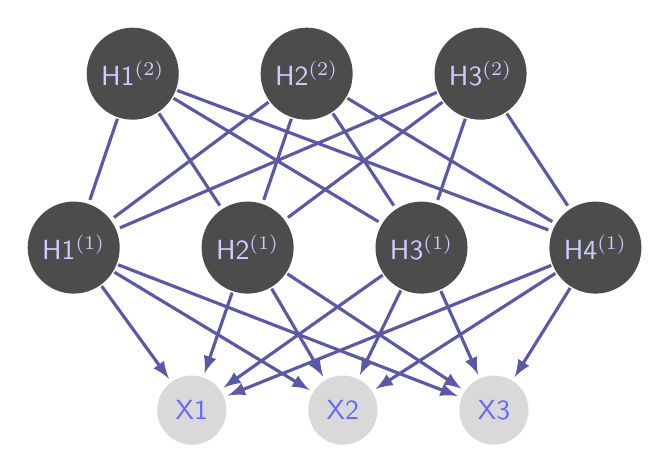
\begin{tikzpicture}[font=\sffamily,node distance=1.cm,->,>=latex,auto,line width=0.4mm]
	
	\tikzset{node st/.style={state, draw=none,
			fill=gray!30!white,
			text=blue!60!white}}
	\tikzset{node obs/.style={state, draw=none,
			fill=gray!60!black,
			text=blue!20!white}}
	
	\node[node obs] (X1) {H1$^{(2)}$};
	\node[node obs, right=of X1] (X2) {H2$^{(2)}$};
	\node[node obs, right=of X2] (X3) {H3$^{(2)}$};
	
	\node[node obs, below=of X1, xshift=-0.75cm] (X11) {H1$^{(1)}$};
	\node[node obs, right=of X11] (X21) {H2$^{(1)}$};
	\node[node obs, right=of X21] (X31) {H3$^{(1)}$};
	\node[node obs, right=of X31] (X41) {H4$^{(1)}$};	
	
	\node[node st, below=of X11, xshift=1.5cm] (Y1) {X1};
	\node[node st, right=of Y1] (Y2) {X2};
	\node[node st, right=of Y2] (Y3) {X3};

	
	\foreach \o in {X11, X21, X31, X41} {
		\foreach \i in {X1, X2, X3} {
			\draw[every loop, auto=right, blue!30!gray] (\i) edge[-] (\o) ; 
		};
	} ;
	
	\foreach \o in {Y1, Y2, Y3} {
		\foreach \i in {X11, X21, X31, X41} {
			\draw[every loop, auto=right, blue!30!gray] (\i) edge[->] (\o);
		};	
	};
	
	\end{tikzpicture}}
\end{center}
We can sample from a DBN via first Gibbs sampling on the undirected layer, then ancestral sampling through the rest of the (directed) model to eventually obtain a sample from the visible units.

\myspace 
\p \blue{Deep Boltzmann Machines} (20.4). Same as DBNs, but now all layers are undirected. Note that this is very close to the standard RBM, since we have a set of hidden and observed variables, except now we interpret certain subgroups of hidden units as being in a ``layer'', thus allowing for connections between hidden units in adjacent layers. What's interesting is that this still defines a bipartite graph, with odd-numbered layers on one side and even on the other\footnote{Recall that this immediately implies that units in all odd layers are conditionally independent given the even layers (and vice-versa for even to odd).}. \\

\myspace
\p \blue{Differentiable Generator Networks} (20.10.2). Use a differentiable function $g(\vec z; \vec{\theta}^{(g)})$ to transform samples of latent variables $\rvec z$ to either (a) samples $\rvec x$, or (b) distributions over samples $\rvec x$. For an example of case (a), the standard procedure for sampling from $\mathcal N(\vec\mu, \matr\Sigma)$ is to first sample from $\mathcal{N}(\vec 0, \matr I)$ into a generator network consisting of a single affine layer:\marginnote{\textbf{Case a}: interpret $g(\vec z)$ as emitting $\vec x$ directly.}[-1em]
$$
	\vec x \leftarrow g(\vec z) = \vec{\mu} + \matr L \vec z
$$
where $\matr L$ is the \textit{Cholesky decomposition}\footnote{The [unique] Cholesky decomposition of a (real-symmetric) p.d. matrix $\matr A$ is a decomposition of the form $\matr A = \matr L \matr L^T$, where $\matr L$ is lower triangular.} of $\matr\Sigma$. In general, we think of the generator function $g$ as providing a change of variables that transforms the distribution over $\rvec z$ into the desired distribution $\rvec x$. Of course, there \textit{is} an exact formula for doing this,
\begin{align}
	p_x(\vec x) 
		&= \frac{ p_z(g^{-1}(\vec x))  }{  \left|  \det \pderiv{g}{\vec z}  \right| }
\end{align}
but it's usually far easier to use indirect means of learning $g$, rather than trying to maximize/evaluation $p_x(\vec x)$ directly. \\

For case (b), the common approach is to train the generator net to emit conditional probabilities\marginnote{\textbf{Case b}: interpret $g(\vec z)$ as emitting $p(\vec x \mid \vec z)$.}[0em]
\begin{align}
	p(x_i \mid \vec z) = g(\vec z)_i \qquad\qquad p(\vec x) = \E[\vec z]{p(\vec x \mid \vec z)}
\end{align}
which can also support generating discrete data (case a cannot). The challenge in training generator networks is that we often have a set of examples $\vec x$, but the value of $\vec z$ for each $\vec x$ is not fixed and known ahead of time. We'll now look at some ways of training generator nets given only training samples for $\vec x$. Note that such a setting is very unlike unsupervised learning, where we typically interpret $\vec x$ as inputs that we don't have labels for, while here we interpret $\vec x$ as \textit{outputs} that we don't know the associated inputs for. 

\myspace 
\p \blue{Variational Autoencoders} (20.10.3). VAEs are directed models that use learned approximate inference and can be trained purely with gradient-based methods. To generate a sample $\vec x$, the VAE first samples $\vec z$ from the \textit{code distribution} $p_{model}(\vec z)$. This sample is then fed through the a differentiable generator network $g(\vec z)$. Finally, $\vec x$ is sampled from $p_{model}(\vec x; g(\vec z)) = p_{model}(\vec x \mid \vec z)$.  























% ==================================================================================
% CONDENSED SUMMARIES
% ==================================================================================
\mysection{Papers and Tutorials}\label{Papers and Tutorials}





% ============================================================================================
\lecture{Papers and Tutorials}{WaveNet}{January 15, 2017}

\p \blue{Abstract}. 
\begin{compactitem}
	\item \textbf{What's WaveNet?} A deep neural network for generating raw audio waveforms.
	\item \textbf{How does it generate them?} \red{IDK}
	\item \textbf{What's it good for?} Text-to-speech, generating music, any waveform really.
\end{compactitem}

\myspace
\p \blue{Introduction}. 
\begin{compactitem}
	\item Inspired by recent advances in \green{neural autoregressive generative models}, and based on the PixelCNN architecture.  
	
	\item Long-range dependencies dealt with via ``dilated causal convolutions, which exhibit very large receptive fields.''
\end{compactitem}

\myspace
\p \blue{WaveNet}. The joint probability of a waveform $x = \{x_1, \ldots, x_T\}$ is factorised as a product of conditional probabilities, 
\begin{align}
p(x) = \prod_{t = 1}^{T} p(x_t \mid x_1, \ldots, x_{t - 1})
\end{align}
which are modeled by a stack of convolutional layers (no pooling).  
\begin{quote}
	The model outputs a categorical distribution over the next value xt with a softmax layer and it is optimized to maximize the log-likelihood of the data w.r.t. the parameters.\\
\end{quote}

\p Main ingredient of WaveNet is \textit{dilated} causal convolutions, illustrated below. Note the absence of recurrent connections, which makes them faster to train than RNNs, but at the cost of requiring many layers,  or large filters to increase the receptive field\footnote{Loose interpretation of receptive fields here is that large fields can take into account more info (back in time) as opposed to smaller fields, which can be said to be ``short-sighted''}. 

\myfig[0.5\textwidth]{CausalConv.PNG}

\p Excellent concise definition from paper:
\begin{quote}
	A dilated convolution (a convolution with holes) is a convolution where the filter is applied over an area larger than its length by skipping input values with a certain step. It is equivalent to a convolution with a larger filter derived from the original filter by dilating it with zeros, but is significantly more efficient. A dilated convolution effectively allows the network to operate on
	a coarser scale than with a normal convolution. This is similar to pooling or strided convolutions, but
	here the output has the same size as the input. As a special case, dilated convolution with dilation
	1 yields the standard convolution.
\end{quote}

\myspace
\p \blue{Softmax distributions}. Chose to model the conditional distributions $p(x_t \mid x_1, \ldots, x_{t -1})$ with a softmax layer. To deal with the fact that there are $2^{16}$ possible values, first apply a ``$\mu$-law companding transformation'' to data, and then quantize it to 256 possible values:
\graybox{
	f(x_t) = \mathrm{sign}(x_t)\frac{\ln(1+\mu|x_t|)}{\ln(1 + \mu)}
	}
which (after plotting in Wolfram) looks identical to the sigmoid function.

\myspace
\p \blue{Gated activation and res/skip connections}. Use the same gated activation unit as PixelCNN:
\begin{align}
z = \tanh\left( W_{f,k} * x \right) ~ \odot ~ \sigma\left( W_{g,k} * x \right)
\end{align}
where $*$ denotes conv operator, $\odot$ denotes elem-wise mult., $k$ is layer index, $f,g$ denote filter/gate, and $W$ is learnable conv filter. This is illustrated below, along with the residual/skip connections used to speed up convergence/enable training deeper models.

\myfig[0.6\textwidth]{WaveNetRes.PNG}

\myspace
\p \blue{Conditional Wavenets}. Can also model conditional distribution of $x$ given some additional $h$ (e.g. speaker identity).
\begin{align}
p(x \mid h) = \prod_{t = 1}^{T} p(x_t \mid x_1, \ldots, x_{t - 1}, h)
\end{align}
\begin{compactitem}[$\rightarrow$]
	\item \textbf{Global conditioning}. Single $h$ that influences output dist. accross all times. Activation becomes:
	\begin{align}
	z = \tanh\left( W_{f,k} * x +  V_{f,k}^T h\right) 
		~ \odot ~ 
		\sigma\left( W_{g,k} * x + V_{g,k}^T h\right)
	\end{align}
	
	\item \textbf{Local conditioning} (confusing). Have a second time-series $h_t$. They first transform this $h_t$ using a ``transposed conv net (learned unsampling) that maps it to a new time-series $y = f(h)$ w/same resolution as $x$. 
\end{compactitem}




\myspace
\p \blue{Experiments}. 
\begin{itemize}
	\item \textbf{Multi-Speaker Speech Generation}. Dataset: multi-speaker corpus of 44 hours of data from 109 different speakers\footnote{Speakers encoded as ID in form of a one-hot vector}. Receptive field of 300 milliseconds.
	
	
	\item \textbf{Text-to-Speech}. Single-speaker datasets of 24.6 hours (English) and 34.8 hours (Chinese) speech. Locally conditioned on \textit{linguistic features}. Receptive field of 240 milliseconds. Outperformed both LSTM-RNN and HMM.
	
	
	\item \textbf{Music}. Trained the WaveNets to model two music datasets: (1) 200 hours of annotated music audio, and (2) 60 hours of solo piano music from youtube. Larger receptive fields sounded more musical.
	
	\item \textbf{Speech Recognition}. ``With WaveNets we have shown that layers of dilated convolutions allow the receptive field to grow longer in a much cheaper way than using LSTM units.''
\end{itemize}

\myspace
\p \blue{Conclusion} (verbatim): ``This paper has presented WaveNet, a deep generative model of audio data that operates directly at the waveform level. WaveNets are autoregressive and combine causal filters with dilated convolutions to allow their receptive fields to grow exponentially with depth, which is important to model the long-range temporal dependencies in audio signals. We have shown how WaveNets can be conditioned
on other inputs in a global (e.g. speaker identity) or local way (e.g. linguistic features). When applied to TTS, WaveNets produced samples that outperform the current best TTS systems in subjective naturalness. Finally, WaveNets showed very promising results when applied to music audio modeling and speech recognition.''




% ============================================================================================
\lecture{Papers and Tutorials}{Neural Style}{January 22}

\p \blue{Notation}. 
\begin{compactitem}
	\item \textbf{Content image}: $\vec{p}$
	\item \textbf{Filter responses}: the matrix $P^l \in \mathcal{R}^{N_l \times M_l}$ contains the activations of the filters in layer $l$, where $P_{ij}^l$ would give the activation of the $i$th filter at position $j$ in layer $l$. $N_l$ is number of feature maps, each of size $M_l$ (height $\times$ width of the feature map)\footnote{If not clear, $M_l$ is a scalar, for any given value of $l$.}.
	\item \textbf{Reconstructed image}: $\vec{x}$ (initially random noise). Denote its corresponding filter response matrix at layer $l$ as $P^l$. 
\end{compactitem}

\myspace
\p \blue{Content Reconstruction}. 
\begin{enumerate}
	\item Feed in \green{content image} $~\vec{p}~$ into pre-trained network, saving any desired filter responses during the forward pass. These are interpreted as the various ``encodings'' of the image done by the network. Think of them analogously to ``ground-truth'' labels.
	
	\item Define $\vec x$ as the \green{generated image}, which we first initialize to random noise. We will be changing the pixels of $\vec x$ via gradient descent updates. 
	
	\item Define the \green{loss function}. After each forward pass, evaluate with squared-error loss between the two representations at the layer of interest:
	\graybox{
		\mathcal{L}_{content}(\vec p, \vec x, l) &= \onehalf \sum_{i, j} (F_{ij}^l - P_{ij}^l)^2 \tlab{1} \\
		\pderiv{\mathcal L_{content}}{F_{ij}^l} &= 
			\begin{cases}
			(F^l - P^l)_{ij} & F_{ij}^l > 0 \\
			0 & F_{ij}^l < 0
		\end{cases}\tlab{2}
		}
	where it appears we are assuming ReLU activations (\red{?}).
	
	\item Compute iterative updates to $\vec x$ via \green{gradient descent} until it generates the same response in a certain layer of the CNN as the original image $\vec p$. 
\end{enumerate}

\myspace
\p \blue{Style Representation}. On top of the CNN responses in each layer, the authors built a style representation that computes the correlations between the different [aforementioned] filter responses. The correlation matrix for layer $l$ is denoted in the standard way with a Gram matrix $G^l \in \mathcal{R}^{N_l \times N_l}$, with entries
\begin{align}
G_{ij}^l &= \langle F^l_i, F_j^l \rangle =  \sum_k F_{ik}^l F_{jk}^l \tlab{3}
\end{align}
To generate a texture that matches the style of a given image, do the following.
\begin{enumerate}
	\item Let $\vec a$ denote the original [style] image, with corresponding $A^l$. Let $\vec x$, initialized to random noise, denote the generated [style] image, with corresponding $G^l$.
	
	\item The contribution to the loss of layer $l$, denoted $E_l$, to the total loss, denoted $\mathcal L_{style}$, is given by
	\graybox{
		E_l &= \frac{1}{4 N_l^2 M_l^2} \sum_{ij} (G_{ij}^l - A_{ij}^l)^2 \tlab{4} \\
		\mathcal L_{style}(\vec a, \vec x) &= \sum_{l = 0}^L w_l E_l \tlab{5} \\
		\pderiv{ E_{l}}{F_{ij}^l} &= 
		\begin{cases}
			\frac{1}{N_l^2 M_l^2}	\left( (F^l)^T (G^l - A^l) \right)_{ji} & F_{ij}^l > 0 \\
			0 & F_{ij}^l < 0
		\end{cases}\tlab{6}
	}
	where $w_l$ are [as of yet unspecified] weighting factors of the contribution of layer $l$ to the total loss. 
\end{enumerate}

\myspace
\p \blue{Mixing content with style}. Essentially a joint minimization that combines the previous two main ideas. 
\begin{enumerate}
	\item Begin with the following images: white noise $\vec x$, content image $\vec p$, and style image $\vec a$. 
	
	\item The loss function to minimize is a linear combination of ~\ref{1} and ~\ref{5}:
	\graybox{
		\mathcal L_{total}(\vec p, \vec a, \vec x, l) 
			&= \alpha \mathcal L_{content}(\vec p, \vec x, l) 
			+ \beta \mathcal L_{style}(\vec a, \vec x) \tlab{7}
		}
	Note that we can choose which layers $L_{style}$ uses by tweaking the layer weights $w_l$. For example, the authors chose to set $w_l = 1/5$ for 'conv[1, 2, 4, 5]\_1' and 0 otherwise. For the ratio $\alpha/\beta$, they explored $1 \times 10^{-3}$ and $1 \times 10^{-4}$.
\end{enumerate}





% ============================================================================================
\lecture{Papers and Tutorials}{Neural Conversation Model}{February 8}
\vspace{-1em}
[{\scriptsize Reminder: \red{red text} means I need to come back and explain what is meant, once I understand it.}]

\p \blue{Abstract}. This paper presents a simple approach for conversational modeling which uses the sequence to sequence framework. It can be trained end-to-end, meaning fewer hand-crafted rules. The \red{lack of consistency} is a common failure of our model. 

\myspace
\p \blue{Introduction}. Major advantage of the seq2seq model is it requires little feature engineering and domain specificity. Here, the model is tested on chat sessions from an IT helpdesk dataset of conversations, as well as movie subtitles.

\myspace
\p \blue{Related Work}. The authors' approach is based on the following (linked and saved) papers on seq2seq:
\begin{compactitem}
	\item \href{https://arxiv.org/pdf/1306.3584.pdf}{Kalchbrenner \& Blunsom, 2013.}
	\item \href{https://arxiv.org/pdf/1409.3215.pdf}{Sutskever et al., 2014.} (Describes Seq2Seq model)
	\item \href{https://arxiv.org/pdf/1409.0473.pdf}{Bahdanau et al., 2014.}
\end{compactitem}

\myspace
\p \blue{Model}. Succinctly described by the authors:\vspace{-1em}
\begin{quote}
	The model reads the input sequence one token at a time, and predicts the output sequence, also one token at a time. During training, the true output sequence is given to the model, so learning can be done by backpropagation. The model is trained to maximize the cross entropy of the correct sequence given
	its context. During inference, in which the true output sequence is not observed, we simply feed the predicted output token as input to predict the next output. This is a “greedy” inference approach. 
\end{quote}
\marginnote{Example of less greedy approach: \red{beam search}.}[-6em]
\myfig[0.8\textwidth]{Seq2SeqModel.PNG}

\myspace
\p The \green{thought vector} is the hidden state of the model when it receives [as input] the end of sequence symbol $\langle eos \rangle$, because it stores the info of the sentence, or \textit{thought}, ``ABC''. The authors acknowledge that this model will \textit{not} be able to ``solve'' the problem of modeling dialogue due to the objective function not capturing the actual objective achieved through human communication, which is typically longer term and based on exchange of information [rather than next step prediction]\marginnote{Ponder: what \textit{would} be a reasonable objective function \& model for conversation?}[-2em]\footnote{I'd imagine that, in order to model human conversation, one obvious element needed would be a \textit{memory}. Reminds me of DeepMind's DNC. There would need to be some online filtering \& output process to capture the crucial aspects/info to store in memory for later, and also some method of retrieving them when needed later. The method for retrieval would likely be some inference process where, given a sequence of inputs, the probability of them being related to some portion of memory could be trained. This would allow for conversations that stretch arbitrarily back in the past. Also, when storing the memories, I'd imagine a reasonable architecture would be some encoder-decoder for a sparse distributed representation of memory.}.

\myspace
\p \blue{IT Data \& Experiment}.\marginnote{Reminder: Check out \href{https://github.com/farizrahman4u/seq2seq}{this git repo}}
\begin{compactitem}
	\item \textbf{Data Description}: Customers talking to IT support, where typical interactions are 400 words long and turn-taking is clearly signaled. 
	
	\item \textbf{Training Data}: 30M tokens, 3M of which are used as validation. They built a vocabulary of the most common 20K words, and introduced special tokens indicating turn-taking and actor.
	
	\item \textbf{Model}: A single-layer LSTM with 1024 memory cells. 
	
	\item \textbf{Optimization}: SGD with gradient clipping.
	
	\item \textbf{Perplexity}: At convergence, achieved \red{perplexity} of 8, whereas an n-gram model achieved 18.
\end{compactitem}

% ============================================================================================
\lecture{Papers and Tutorials}{NMT By Jointly Learning to Align \& Translate}{February 27}

\href{https://arxiv.org/abs/1409.0473}{[Bahdanau et. al, 2014]}. The primary motivation for me writing this is to better understand the \green{attention mechanism} in my sequence to sequence chatbot implementation.

\myspace
\p \blue{Abstract}. The authors claim that using a fixed-length vector [in the vanilla encoder-decoder for NMT] is a bottleneck. They propose allowing a model to (soft-)search for parts of a source sentence that are relevant to predicting a target word, without having to form these parts as a hard segment explicitly.

\myspace
\p \blue{Learning to Align\footnote{By ``align'' the authors are referring to aligning the source-search to the relevant parts for prediction.} and translate}. 
\begin{itemize}
	\item \textbf{Decoder}. Their encoder defines the conditional output distribution as
	\begin{align}
		p(y_i \mid y_1, \ldots, y_{i - 1}, \vec{x}) &= g(y_{i - 1}, s_i, c_i) \\
		s_i &= f(s_{i - 1}, y_{i - 1}, c_i)
	\end{align}
	where $s_i$ is the RNN [decoder] hidden state at time $i$. 
	\begin{compactitem}
		\item NOTE: $c_i$ is \textit{not} the $i$th element of the standard context vector; rather, it is \textit{itself} a distinct context vector that depends on a sequence of \green{annotations} $(h_1, \ldots, h_{T_x})$. It seems that each annotation $h_i$ is a hidden (encoder) state ``that contains information about the whole input sequence with a strong focus on the parts surrounding the i-th word of the input sequence.''
		
		\item The context vector $c_i$ is computed as follows:
		\begin{align}
			c_i &= \sum_{j = 1}^{T_x} \alpha_{ij} h_j \\
			\alpha_{ij} &= \frac{\exp(e_{ij})}{\sum_{k = 1}^{T_x} \exp(e_{ik})} \\
			e_{ij} &= a(s_{i - 1}, h_j) 
		\end{align}
		where the function $e_{ij}$ is given by an \green{alignment model} which scores how well the inputs around position $j$ and the output at position $i$ match. 
	\end{compactitem}
	
	
	\item \textbf{Encoder}. It's just a bidirectional RNN. What they call ``annotation $h_j$'' is literally just a concatenated vector of $h_j^{forward}$ and $h_j^{backward}$
\end{itemize}


\myspace
\subsub{Detailed Model Architecture}

(Appendix A). Explained with the TensorFlow user in mind.\\

\myspace
\p \blue{Decoder Internals}. It's just a GRU. However, it will be helpful to detail how we format the inputs (given we now have attention). Wherever we'd usually pass the previous decoder state $s_{i - 1}$, we now pass a \textit{concatenated} state, $[s_{i - 1},~ c_i]$, that also contains the $i$th context vector. Below I go over the flow of information from GRU input to output:
\begin{compactenum}
	\item \textbf{Notation}: $y_t$ is the loop-embedded \underline{output} of the decoder (prediction) at time $t$, $s_t$ is the internal hidden state of the decoder at time $t$, and $c_t$ is the context vector at time $t$. $\tilde s_t$ is the proposed/proposal state at time $t$.
	\item \textbf{Gates}:
	\begin{align}
		z_t &= \sigma\left( W_z y_{t - 1} + U_z [s_{t - 1},~ c_t] \right)
		\qquad \mgreen{\text{[update gate]}} \\
		r_t &= \sigma\left( W_r y_{t - 1} + U_r [s_{t - 1},~ c_t] \right)
		\qquad \mgreen{\text{[reset gate]}} \\
	\end{align}
		
	\item \textbf{Proposal state}:
	\begin{align}
		\tilde s_t &= \tanh\left( W y_{t - 1} + U [r_t \circ s_{t - 1}, ~ c_t]  \right)
	\end{align}
	
	\item \textbf{Hidden state}:
	\begin{align}
		s_t &= (1 - z_t) \circ s_{t - 1} + z_t \circ \tilde s_t
	\end{align}
	
\end{compactenum}

\myspace 
\p \blue{Alignment Model}. All equations enumerated below are for some timestep $t$ during the decoding process.
\begin{compactenum}
	\item \textbf{Score}: For all $j \in [0, L_{enc}-1]$ where $L_{enc}$ is the number of words in the encoder sequence, compute:
	\begin{align}
		a_j = a(s_{t - 1}, h_j) &= v_a^T \tanh\left( W_a s_{t - 1} + U_a h_j \right)
	\end{align}
	
	\item \textbf{Alignments}: Feed the unnormalized alignments (scores) through a softmax so they represent a valid probability distribution.
	\begin{align}
		a_j \leftarrow \frac{e^{a_j}}{\sum_{k = 0}^{L_{enc}-1} e^{a_k}}
	\end{align}
	
	\item \textbf{Context}: The context vector input for our decoder at this timestep:
	\begin{align}
		c = \sum_{j = 1}^{L_{enc}} a_j h_j
	\end{align}
\end{compactenum}

\myspace
\p \blue{Decoder Outputs}. All below is for some timestep $t$ during the decoding process. To find the probability of some (one-hot) word $y$ [at timestep $t$]:
\begin{align}
	\Pr\left(y \mid s, c \right) &\propto e^{y^T W_o u} \\
	u &= \left[\max\{ \tilde u_{2j - 1}, \tilde u_{2j} \}\right]_{j = 1,\ldots, \ell}^T \\
	\tilde u &= U_o [s_{t - 1}, ~ c] + V_o y_{t - 1}
\end{align}
\red{N.B.}: From reading other (and more recent) papers, these last few equations do not appear to be the way it is usually done (thank the lord). See Luong's work for a much better approach.

% ==============================================================================
% ==============================================================================
\lecture{Papers and Tutorials}{Effective Approaches to Attention-Based NMT}{May 11}
% ==============================================================================
% ==============================================================================

\href{https://arxiv.org/abs/1508.04025}{[Luong et. al, 2015]}

\p \blue{Attention-Based Models}. For attention especially, the devil is in the details, so I'm going to go into somewhat excruciating detail here to ensure no ambiguities remain. For both global and local attention, the following information holds true:
\begin{compactitem}
	\item ``At each time step t in the decoding phase, both approaches first take as input the hidden state $\vec[t]{h}$ at the top layer of a stacking LSTM.'' 
	\item Then, they derive [with different methods] a context vector $\vec[t]{c}$ to capture source-side info.
	\item Given $\vec[t]{h}$ and $\vec[t]{c}$, they both compute the \green{attentional hidden state} as:
	\graybox{
		\vec[t]{\tilde h} &= \tanh\left(  \matr[c]{W} [\vec[t]{c};~ \vec[t]{h}]   \right)
		}
		
	\item Finally, the predictive distribution (decoder outputs) is given by feeding this through a softmax:
	\begin{align}
		p(y_t \mid y_{<t}, x) &= \text{softmax}\left(  \matr[s]{W} \vec[t]{\tilde h}   \right)
	\end{align}
\end{compactitem}

\myspace
\p \blue{Global Attention}. Now I'll describe in detail the processes involved in $\vec[t]{h} \rightarrow  \vec[t]{a} \rightarrow \vec[t]{c} \rightarrow   \vec[t]{\tilde h}$.
\begin{compactenum}
	\item $\vec[t]{h}$: Compute the hidden state $\vec[t]{h}$ in the normal way (not obvious if you've read e.g. Bahdanau's work...)
	
	\item $\vec[t]{a}$: 
	\begin{compactenum}
		\item Compute the \green{scores} between $\vec[t]{h}$ and each source $\vec[s]{\bar h}$, where our options are:
		\graybox{
			\text{score}(\vec[t]{h}, \vec[s]{\bar h}) 
			&= \begin{cases}
				\vec[t]{h}^T \vec[s]{\bar h} & \mgreen{dot} \\
				\vec[t]{h}^T \matr[a]{W} \vec[s]{\bar h} & \mgreen{general} \\
				\vec[a]{v}^T \tanh\left(\matr[a]{W} [\vec[t]{h}; ~ \vec[s]{\bar h}] \right) & \mgreen{concat} 
			\end{cases}
			}
			
		\item Compute the \green{alignment vector} $\vec[t]{a}$ of length $L_{enc}$ (number of words in the encoder sequence):
		\begin{align}
			\vec[t]{a}(s) &= \text{align}(\vec[t]{h}, \vec[s]{\bar h}) \\
			&= \frac{\exp(\text{score}(\vec[t]{h}, \vec[s]{\bar h}) )}{
				\sum_{s'} \exp(\text{score}(\vec[t]{h}, \vec[s']{\bar h}) )
				}
		\end{align}
	\end{compactenum}
	
	\item $\vec[t]{c}$: The weighted average over all source (encoder) hidden states\footnote{NOTE: Right after mentioning the context vector, the authors have the following cryptic footnote that may be useful to ponder: \textit{For short sentences, we only use the top part of
		$a_t$ and for long sentences, we ignore words near the end}.}:
	\begin{align}
		\vec[t]{c} &= \sum_{i = 1}^{L_{enc}} \vec[t]{a}(i) \vec[i]{\bar h}
	\end{align}
	
	\item $\vec[t]{\tilde h}$: For convenience, I'll copy the equation for $\vec[t]{\tilde h}$ again here:
	\begin{align}
		\vec[t]{\tilde h} &= \tanh\left(  \matr[c]{W} [\vec[t]{c};~ \vec[t]{h}]   \right)
	\end{align}
\end{compactenum}

\myspace
\p \blue{Input-Feeding Approach}. A copy of each output $\vec[t]{\tilde h}$ is sent forward and concatenated with the inputs for the next timestep, i.e. the inputs go from $\vec[t+1]{x}$ to $[\vec[t]{\tilde h}; \vec[t+1]{x}]$. 


% ==============================================================================
% ==============================================================================
 \lecture{Papers and Tutorials}{Using Large Vocabularies for NMT}{March 11}
% ==============================================================================
% ==============================================================================

\p Paper information:
\begin{compactitem}[-]
	\item Full title: On Using Very Large Target Vocabulary for Neural Machine Translation. 
	\item Authors: Jean, Cho, Memisevic, Bengio.
	\item Date: 18 Mar 2015. 
	\item \href{https://arxiv.org/abs/1412.2007}{[arXiv link]}
\end{compactitem}


\myspace
\p \blue{NMT Overview}. Typical implementation is encoder-decoder network. Notation for inputs \& encoder:
\begin{align}
x &= (x_1, \ldots, x_T)
\qquad \mgreen{\text{[source sentence]}} \\
h &= (h_1, \ldots, h_T)
\qquad \mgreen{\text{[encoder state seq]}} \\
h_t &= f(x_t, h_{t - 1}) \label{h}
\end{align}
where $f$ is the function defined by the \textit{cell state} (e.g. GRU/LSTM/etc.). Then the decoder generates the output sequence $y$, and with probability given below:\marginnote{The functions $q$, $g$, and $r$ are just placeholders -- ``some function of [inputs].''}[2em]
\begin{align}
y &= (y_1, \ldots, y_T') \qquad \mgreen{[y_i \in \mathbb{Z}]} \\
\Pr[y_t \mid y_{<t}, ~ x] &\propto e^{q(y_{t-1},~ z_t, ~ c_t)}  \label{y}\\
z_t &= g(y_{t - 1}, z_{t - 1}, c_t) 
\qquad \mred{\text{[decoder hidden?]}} \label{z} \\
c_t &= r(z_{t - 1}, h_1, \ldots, h_T) 
\qquad \mred{\text{[decoder inp?]}} \label{c}
\end{align}
As usual, model is jointly trained to maximize the conditional log-likelihood of correct translation. For $N$ training sample pairs $(x^n, y^n)$, and denoting the length of the $n$-th target sentence as $T_n$, this can be written as,
\begin{align}
\theta^* &= \argmax_\theta \sum_{n = 1}^{N} \sum_{t = 1}^{T_n}
\log\left(\Pr[y_t^n \mid y_{<t}^n, ~ x^n]  \right)
\end{align}

\myspace
\p \blue{Model Details}. Above is the general structure. Here I'll summarize the specific model chosen by the authors. 
\begin{compactitem}
	\item \textbf{Encoder}. Bi-directional, which just means $h_t = \left[h_t^{backward};~h_t^{forward} \right]$. The chosen cell state (the function $f$) is GRU.
	
	\item \textbf{Decoder}. At each timestep, computes the following:
	\begin{compactitem}[$\rightarrow$]
		\item \green{Context vector $c_t$}. \marginnote{$a$ is a standard single-hidden-layer NN.}[7em]
		\begin{align}
		c_t &= \sum_{i = 1}^{T} \alpha_i h_i \\
		\alpha_t &= \dfrac{e^{a(h_t, z_{t - 1})}}{\sum_k e^{a(h_k, z_{t - 1}})} 
		\end{align}
		\item \green{Decoder hidden state $z_t$}. Also a GRU cell. Computed based on the previous hidden state $z_{t - 1}$, the previously generated symbol $y_{t - 1}$, and also the computed context vector $c_t$. 
	\end{compactitem}
	
	\item \textbf{Next-word probability}. They model equation ~\ref{y} as\footnote{Note: The formula for $Z$ is correct. Notice that the only part of the RHS of Pr($y_t$) with a $t$ is as the subscript of $w$. To be clear, $w_k$ is a full word vector and the sum is over all words in the output \textit{vocabulary}, the index $k$ has absolutely nothing to do with timestep. They use the word target but make sure not to misinterpret that as somehow meaning target words in the sentence or something.} ,\marginnote{Reminder: $y_i$ is an integer token, while $\rvec[i]{w}$ is the target vector of length vocab size}
	\begin{align}
	\Pr[y_t \mid y_{<t}, ~ x]  &= \frac{1}{Z} e^{\rvec[t]{w}^T \phi(y_{t - 1}, z_t, c_t) + b_t} \\
	Z &= \sum_{k:~y_k\in V}    e^{\rvec[k]{w}^T \phi(y_{t - 1}, z_t, c_t) + b_k}
	\end{align}
	where $\phi$ is affine transformation followed by a nonlinear activation, $\rvec[t]{w}$ and $b_t$ are the \green{target word vector} and bias. $V$ is the set of all target \textit{vocabulary}. 
\end{compactitem}

\myspace
\p \blue{Approximate Learning Approach}. Main idea:
\vspace{-1em}
\begin{center}
	\begin{quote}
		{\footnotesize ``In order to avoid the growing complexity of computing the normalization constant, we propose here to use only a small subset $V'$ of the target vocabulary at each update.''}
	\end{quote}
\end{center}
Consider the gradient of the log-likelihood\footnote{\red{NOTE TO SELF}: After long and careful consideration, I'm concluding that the authors made a typo when defining $\mathcal{E}(y_j)$, which they choose to subscript all parts of the RHS with $j$, but that is in direct contradiction with a step-by-step derivation, which is why I have written it the way it is. I'm pretty sure my version is right, but I know you'll have to re-derive it yourself next time you see this. And you'll somehow prove me wrong. Actually, after reading on further, I doubt you'll prove me wrong. Challenge accepted, me. Have fun!}, written in terms of the energy $\mathcal{E}$. 
\begin{align}
\nabla \log\left(\Pr[y_t \mid y_{<t}, ~ x]  \right)
&= \nabla \mathcal{E}(y_t) 
- \sum_{k:~y_k\in V}\Pr[y_k \mid y_{<t}, ~ x]\nabla\mathcal{E}(y_k)\\
\mathcal{E}(y_j) &= \rvec[j]{w}^T \phi(y_{t - 1}, z_t, c_t) + b_j
\end{align}


\myspace
\p The crux of the approach is interpreting the second term as $\mathbb{E}_P\left[\nabla \mathcal{E}(y) \right]$, where $P$ denotes $Pr(y \mid y_{<t}, x)$. They approximate this expectation by taking it over a \underline{subset} $V'$ of the predefined proposal \underline{distribution} $Q$. So $Q$ is a p.d.f. over the possible $y_i$, and we sample \textit{from} $Q$ to generate the elements of the subset $V'$. 
\graybox{
	\mathbb{E}_P\left[\nabla \mathcal{E}(y) \right] 
	&\approx \sum_{k:~y_k\in V'} \dfrac{\omega_k}{
		\sum_{k':y_{k'}\in V'} \omega_{k'} } \nabla\mathcal{E}(y_k)\\
	\omega_k &= e^{\mathcal{E}(y_k) - \log Q(y_k)}
}

Here is some math I did that was illuminating to me; I'm not sure why the authors didn't point out these relationships. 
\begin{align}
&\omega_k = \frac{e^{\mathcal{E}(y_k)}}{Q(y_k)} 
\quad\text{thus}\quad
p(y_k \mid y_{<t}, x) = \omega_k \frac{Q(y_k)}{Z} \\
\rightarrow~~  &e^{\mathcal{E}(y_k)} = Z \cdot p(y_k \mid y_{<t}, x) 
= Q(y_k) \cdot \omega_k
\end{align}

\redbox[Now \textit{check this out}]{
	Below are the exact and approximate formulas for $\mathbb{E}_P\left[\nabla \mathcal{E}(y) \right]$ written in a \sout{seductive} suggestive manner. Pay careful attention to subscripts and primes.
	\begin{align}
	\mathbb{E}_P\left[\nabla \mathcal{E}(y) \right] 
	&=  \sum_{k:~y_k\in V} \dfrac{ \omega_k \cdot Q(y_k) }{ 
		\sum_{k':y_{k'}\in V} \omega_{k'} \cdot Q(y_{k'}) }  
	\nabla\mathcal{E}(y_k)\\
	\mathbb{E}_P\left[\nabla \mathcal{E}(y) \right] 
	&=  \sum_{k:~y_k\in V'} \dfrac{ \omega_k }{  \sum_{k':y_{k'}\in V'} \omega_{k'} }  \nabla\mathcal{E}(y_k)
	\end{align}
	They're almost the same! It's much easier to see why when written this way. I interpret the difference as follows: in the exact case, we explicitly attach the probabilities $Q(y_k)$ and sum over all values in $V$. In the second case, by sampling a subset $V'$ from $Q$, we have encoded these probabilities implicitly as the relative frequency of elements $y_k$ in $V'$
}

\myspace
\p \blue{How to do in practice (very important)}. 
\begin{center}
	\begin{quote}
		``In practice, we partition the training corpus and define a subset $V'$ of the target vocabulary for each partition prior to training. Before training begins, we sequentially examine each target sentence in the training corpus and accumulate
		unique target words until the number of unique target words reaches the predefined threshold $\tau$. The accumulated vocabulary will be used for this partition of the corpus during training. We repeat this until the end of the training set is reached. Let us refer to the subset of target words used for the i-th partition by $V'_i$.
	\end{quote}
\end{center}




% ============================================================================================
% ============================================================================================
\lecture{Papers and Tutorials}{Candidate Sampling -- TensorFlow}{March 19}
% ============================================================================================
% ============================================================================================

{\scriptsize \href{https://www.tensorflow.org/extras/candidate_sampling.pdf}{[Link to article]}}

\myspace
\blue{What is Candidate Sampling} The goal is to learn a compatibility function $F(x, y)$ which says something about the compatibility of a class $y$ with a context $x$. Candidate sampling: for each training example $(x_i, y_i)$, only need to evaluate $F(x, y)$ for a small set of classes $\{C_i\} \subset \{L\}$, where $\{L\}$ is the set of all possible classes (vocab size number of elements). We represent $F(x, y)$ as a \textit{layer that is trained by back-prop from/within the loss function}. 

\myspace
\p \blue{C.S. for Sampled Softmax}. I'll further narrow this down to my use case of having exactly 1 target class (word) at a given time. Any other classes are referred to as \green{negative} classes (for that example). 

\myspace
\p \blue{Sampling algorithm}. For each training example $(x_i, y_i)$, do:
\begin{compactitem}
	\item Sample the subset $S_i \subset L$. How? By sampling from $Q(y|x)$ which gives the probability of any particular $y$ being included in $S_i$. 
	
	\item Create the set of \green{candidates}, which is just $C_i := S_i \cup y_i$. 
\end{compactitem}

\myspace
\p \blue{Training task}. We are given this set $C_i$ and want to find out which element of $C_i$ is the target class $y_i$. In other words, we want the posterior probability that any of the $y$ in $C_i$ are the target class, given what we know about $C_i$ and $x_i$. We can evaluate and rearrange as usual with Bayes' rule to get:
\graybox{
	\Pr\left(y^{true}_i = y \mid C_i, ~ x_i \right) 
	&= 
		\dfrac{\Pr\left(y^{true}_i = y \mid x_i \right) 
			\cdot \Pr\left( C_i \mid y^{true}_i = y, ~ x_i \right)
			}{
			\Pr\left(C_i \mid x_i\right) 
		} \\
	%
	&= 
		\frac{\Pr\left(y\mid x_i\right)}{Q\left(y\mid x_i\right)} 
		\cdot 
		\frac{1}{K(x_i, C_i)}  \label{candform}
}
where they've just defined 
\begin{align}
	K(x_i, C_i) \triangleq \frac{ \Pr\left(C_i \mid x_i \right) }{
		\prod_{y'\in C_i} Q(y' \mid x_i)
		\prod_{y'\in(L - C_i)} \left( 1 - Q(y' \mid x_i)\right)
		}
\end{align}

\myspace
\p \blue{Clarifications}. 
\begin{itemize}
	\item The learning function $F(x, y)$ is the \textit{input} to our softmax. \underline{It is our neural network}, excluding the softmax function. 
	
	\item After training our network, it should have learned the general form
	\begin{align}
		F(x, y) = \log( \Pr( y \mid x) )  + 
		K(x) \label{Fxy}
	\end{align}
	which is the general form because
	\begin{align}
		\text{Softmax}(\log(\Pr(y \mid x)) + K(x)) 
		&= 
		\frac{ e^{\log(\Pr(y \mid x)) + K(x)}   }{
			\sum_{y'} e^{\log(\Pr(y' \mid x) + K(x) }} \\
		&= \Pr(y \mid x)	
	\end{align}
	Note that I've been a little sloppy here, since $\Pr(y \mid x)$ up until the last line actually represented the (possibly) unnormalized/\textit{relative} probabilities. 
	
	\item {\footnotesize \red{[MAIN TAKEAWAY]}}. Time to bring it all together. Notice that we've only trained $F(x, y)$ to include \textit{part} of what's needed to compute the probability of any $y$ being the target given $x_i$ \underline{and $C_i$} \textellipsis equation ~\ref{Fxy} doesn't take into account $C_i$ at all! Luckily we know the form of the full equation because it just the log of equation ~\ref{candform}. We can easily satisfy that by subtracting $\log(Q(y\mid x))$ from $F(x, y)$ right before feeding into the softmax. \\
	
	\p\textbf{TL;DR}. Train network to learn $F(x, y)$ before softmax, but instead of feeding $F(x, y)$ to softmax directly, feed 
	\graybox{
		\text{Softmax Input: } F(x, y) - \log(Q(y\mid x))
		}
	instead. That's it.
\end{itemize}




% ==========================================================================
\lecture{Papers and Tutorials}{Attention Terminology}{April 04}
%===========================================================================

Generally useful info. Seems like there are a few notations floating around, and here I'll attempt to set the record straight. The order of notes here will loosely correspond with the order that they're encountered going from encoder output to decoder output.\\

\myspace
\p \blue{Jargon}. The people in the attention business \textit{love} obscure names for things that don't need names at all. Terminology:
\begin{compactitem}
	\item \textbf{Attentions keys/values}: Encoder output sequence.
	\item \textbf{Query}: Decoder [cell] state. Typically the most recent one.
	\item \textbf{Scores}: Values of $e_{ij}$. For the Bahdanau version, in code this would be computed via
	\begin{align}
		e_i &= v^T \tanh(\text{FC}(s_{i - 1}) + \text{FC}(h))
	\end{align}
	where we'd have FC be tf.layers.fully\_connected with num\_outputs equal to our attention size (up to us). Note that $v$ is a vector.
	\item \textbf{Alignments}: output of the softmax layer on the attention scores. 
	\item \textbf{Memory}: The $\alpha$ matrix in the equation $c_i = \sum_{j = 1}^{T_x} \alpha_{ij} h_j$.
\end{compactitem}

\myspace
\p When someone lazily calls some layer output the ``attention'', they are usually referring to the layer \textit{just after} the linear combination/map of encoder hidden states. You'll often see this as some vague function of the previous decoder state, context vector, and possibly even decoder output (after project), like $f(s_{i - 1}, y_{i - 1}, c_i)$. In 99.9\% of cases, this function is just a fully connected layer (if even needed) to map back to the state size for decoder input. That is it.


\p \blue{From encoder to decoder}. The path of information flow from encoder outputs to decoder inputs, a non-trivial process that isn't given the \textit{attention} (heh) it deserves\footnote{For some reason, the literature favors explaining the path ``backwards'', starting with the highly abstracted ``decoder inputs as a weighted sum of encoder states'' and then breaking down what the weights are. Unfortunately, the weights are computed via a multi-stage process so that becomes very confusing very quick.}
\begin{enumerate}
	\item \textbf{Encoder outputs}. Tensor of shape \purple{[batch size, sequence length, state size]}. The state is typically some RNNCell state.
	\begin{compactitem}
		\item Note: TensorFlow's AttenntionMechanism classes will actually convert this to \purple{[batch size, $L_{enc}$, attention size]}, and refer to it as the ``memory''. It is also what is returned when calling myAttentionMech.values. 
	\end{compactitem}
	
	
	\item \textbf{Compute the scores}. The attention scores are the computation described by Luong/Bahdanau techniques. They both take an inner product of sorts on \textit{copies} of the encoder outputs and decoder previous state (query). The main choices are:
	\begin{align}
				\text{score}(\vec[t]{h}, \vec[s]{\bar h}) 
				&= \begin{cases}
				\vec[t]{h}^T \vec[s]{\bar h} & \mgreen{dot} \\
				\vec[t]{h}^T \matr[a]{W} \vec[s]{\bar h} & \mgreen{general} \\
				\vec[a]{v}^T \tanh\left(\matr[a]{W} [\vec[t]{h}; ~ \vec[s]{\bar h}] \right) & \mgreen{concat} 
				\end{cases}
	\end{align}
	where the shapes are as follows (for single timestep during decoding process):\marginnote{\green{Synonyms:\\ - scores \\
			 - unnormalized alignments}}[-5em]
	\begin{compactitem}
		\item $\vec[s]{\bar h}$: \purple{[batch size, 1, state size]}
		\item $\vec[t]{h}$: \purple{[batch size, 1, state size]}
		\item $\matr[a]{W}$: \purple{[batch size, state size, state size]}
		\item $\text{score}(\vec[t]{h}, \vec[s]{\bar h})$: \purple{[batch size]}
	\end{compactitem}
		
	\item \textbf{Softmax the scores}. In the vast majority of cases, the attention scores are next fed through a softmax to convert them into a valid probability distribution. Most papers will call this some vague probability function, when in reality they are using softmaxonly.\marginnote{ \green{Synonyms:\\
				- softmax outputs \\
				- attention dist. \\
				- alignments}}[-3.5em]
	\begin{align}
	\vec[t]{a}(s) &= \text{align}(\vec[t]{h}, \vec[s]{\bar h}) \\
	&= \frac{\exp(\text{score}(\vec[t]{h}, \vec[s]{\bar h}) )}{
		\sum_{s'} \exp(\text{score}(\vec[t]{h}, \vec[s']{\bar h}) )
	}
	\end{align}
	where the alignment vector $\vec[t]{a}$ has shape \purple{[batch size, $L_{enc}$]}
		
	\item \textbf{Compute the context vector}. The inner product of the softmax outputs and the raw encoder outputs.\marginnote{\green{Synonyms:\\ 
			- context vector\\
			- attention}}[-1em]
	This will have shape \purple{[batch size, attention size]} in TensorFlow, where attention size is from the constructor for your AttentionMechanism.
	
	\item \textbf{Combine context vector and decoder output}: Typically with a concat. \textit{The result is what people mean when they say ``attention''}. Luong et al. denotes this as $\vec[t]{\tilde h}$, the decoder output at timestep $t$. This is what TensorFlow means by ``Luong-style mechanisms output the attention.'' And yes, these are used (at least for Luong) to compute the prediction:
	\graybox{
		\vec[t]{\tilde h} &= \tanh\left( \matr[c]{W}\left[
			\vec[t]{c}, ~ \vec[t]{h}
		 \right]   \right) \\
		 p( y_t \mid y_{<t}, x  ) &= \text{softmax}(
			 \matr[s]{W}  \vec[t]{\tilde h}
		 )
		}
\end{enumerate}










% ============================================================================================
% ============================================================================================
\lecture{Papers and Tutorials}{TextRank}{May 03}
% ============================================================================================
% ============================================================================================

\myspace
\p \blue{Introduction}. A graph-based ranking algorithm is a way of deciding on the importance of a vertex within a graph, by taking into account global information recursively computed from the entire graph, rather than relying only on local vertex-specific information.\marginnote{\textbf{Semantic graph}: one whose structure encodes meaning between the nodes (semantic elements).}[-2em] \green{TextRank} is a graph-based ranking model for graphs extracted from natural language texts. The authors investigate/evaluate TextRank on unsupervised keyword and sentence extraction.

\myspace
\p \blue{The \sout{TextRank} PageRank Model}. In general [graph-based ranking], a vertex can be ranked based on certain properties such as the number of vertices pointing to it (in-degree), how highly-ranked \textit{those} vertices are, etc. Formally, the authors [of \textit{PageRank}] define the score of a vertex $V_i$ as follows:\marginnote{The factor $d$ is usually set to 0.85.}[2em]

\graybox{
	S(V_i) &= (1 - d) + d * \sum_{V_j \in \textrm{In}(V_i)} \frac{1}{\mid \textrm{Out}(V_i) \mid} S(V_j) 
	\quad \text{where} \quad 
	d \in \Re[0, 1]} \label{textrank-formula}
and the damping factor $d$ is interpreted as the probability of jumping from a given vertex\footnote{Note that $d$ is a single parameter for the graph, i.e. it is the same for all vertices.} to another \underline{random} vertex in the graph. In practice, the algorithm is implemented through the following steps:
\begin{compactitem}
	\item[(1)] Initialize all vertices with arbitrary values.\footnote{The authors do not specify what they mean by arbitrary. What range? What sampling distribution? Arbitrary as in uniformly random? \red{EDIT}: The authors claim that the vertex values upon completion are not affected by the choice of initial value. Investigate!}
	
	\item[(2)] Iterate over vertices, computing equation~\ref{textrank-formula} until convergence [of the error rate] below a predefined threshold. The error-rate, defined as the difference between the "true score" and the score computed at iteration $k$, $S^k(V_i)$, is \textit{approximated} as:
	\begin{align}
		\textrm{Error}^k(V_i) \approx S^{k}(V_i) - S^{k - 1}(V_i)
	\end{align}
\end{compactitem}

\myspace 
\p \blue{Weighted Graphs}. In contrast with the PageRank model, here we are concerned with natural language texts, which may include multiple or partial links between the units (vertices). The authors hypothesize that modifying equation~\ref{textrank-formula} to incorporate \textit{weighted} connections may be useful for NLP applications.\marginnote{$w_{ij}$ denotes the connection between vertices $V_i$ and $V_j$.}[2em]

\graybox{
	\textcolor{OliveGreen}{W}S(V_i) &= (1 - d) + d * \sum_{j \in \textrm{In}(V_i)}
		\textcolor{OliveGreen}{
			 \frac{w_{ji}}{ \sum{V_k \in \textrm{Out}(V_j)} w_{jk} }
			W }
	S(V_j) \label{textrank-formula-2}
}
where I've shown the modified part in green. The authors mention they set all weights to random values in the interval 0-10 (no explanation). 

\myspace
\p \blue{Text as a Graph}. In general, the application of graph-based ranking algorithms to natural language texts consists of the following main steps:
\begin{compactitem}
	\item[(1)] Identify text units that best define the task at hand, and add them as vertices in the graph.
	
	\item[(2)] Identify relations that connect such text unit in order to draw edges between vertices in the graph. Edges can be directed or undirected, weighted or unweighted.
	
	\item[(3)] Iterate the algorithm until convergence.\vspace{0.3em}
	
	\item[(4)] Sort [in reversed order] vertices based on final score. Use the values attached to each vertex for ranking/selection decisions.
\end{compactitem}

\myspace\Needspace{30\baselineskip}
\subsub{Keyword Extraction}
\myspace

\p \blue{Graph}. The authors apply TextRank to extract words/phrases that are representative for a given document. The individual graph components are defined as follows:
\begin{compactitem}[-]
	\item \green{Vertex}: sequence of one or more lexical units from the text.
	\begin{compactitem}
		\item In addition, we can restrict which vertices are added to the graph with \underline{syntactic filters}.
		\item Best filter [for the authors]: \textit{nouns and adjectives only}.
	\end{compactitem}
	\item \green{Edge}: two vertices are connected if their corresponding lexical units co-occur within a window of $N$ words\marginnote{Typically $N \in \Z[2, 10]$}[-1em]\footnote{That is \textellipsis  simpler than expected. \textit{Can we do better?}}.
\end{compactitem}

\myspace\Needspace{15\baselineskip}
\p \blue{Procedure}:
\begin{compactitem}
	\item[(1)] \textbf{Pre-Processing}: Tokenize and annotate [with POS] the text.\vspace{0.3em}
	
	\item[(2)] \textbf{Build the Graph}: Add all [single] words to the graph that pass the syntactic filter, and connect [undirected/unweighted] edges as defined earlier (co-occurrence).
	
	\item[(3)] \textbf{Run algorithm}: Initialize all scores to 1. For a convergence threshold of 0.0001, usually takes about 20-30 iterations.
	
	\item[(4)] \textbf{Post-Processing}: 
	\begin{compactitem}
		\item[(i)] Keep the top $T$ vertices (by score), where the authors chose $T = |V|/3$.\footnote{Another approach is to have $T$ be a fixed value, where typically $5 < T < 20$.} Remember that vertices are still individual words.
		
		\item[(ii)] From the new subset of $T$ keywords, collapse any that were adjacent in the original text in a single lexical unit.
	\end{compactitem}
\end{compactitem}

\myspace
\p \blue{Evaluation}. The data set used is a collection of 500 abstracts, each with a set of keywords. Results are evaluated using \green{precision}, \green{recall}, and \green{F-measure}\footnote{
	Brief terminology review:
	\begin{compactitem}
		\item \green{Precision}: fraction of keywords extracted that are in the "true" set of keywords.
		\item \green{Recall}: fraction of "true" keywords that are in the extracted set of keywords.\marginnote{A PR Curve plots precision as a function of recall.}[-2em]
		\item \green{F-score}: combining precision and recall to get a single number for evaluation:
		$$
		F = \frac{2pr}{p + r}
		$$
	\end{compactitem}
	}. % end footnote
The best results were obtained with a co-occurrence window of 2 [on an undirected graph], which yielded:
$$
\text{Precision: } 31.2\% \quad \text{Recall: } 43.1\% \quad \text{F-measure: } 36.2
$$
The authors found that larger window size corresponded with lower precision, and that directed graphs performed worse than undirected graphs.

\myspace
\subsub{Sentence Extraction} 
\myspace 

\p \blue{Graph}. Now we move to ``sentence extraction for automatic summarization.''
\begin{compactitem}
	\item \green{Vertex}: a vertex is added to the graph for each sentence in the text.
	\item \green{Edge}: each weighted edge represents the similarity between two sentences. The authors use the following similarity measure between two sentences $S_i$ and $S_j$:
	\graybox{
		\textrm{Similarity}(S_i, S_j) &= 
			\frac{\mid S_i \cap S_j \mid}{\log(\mid S_i \mid) + \log(\mid S_j \mid)}
		}
		where the numerator is the number of words that occur in both $S_i$ and $S_j$. 
\end{compactitem}
The \blue{procedure} is identical to the algorithm described for keyword extraction, except we run it on full sentences.

\myspace
\p \blue{Evaluation}. The data set used is 567 news articles. For each article, TextRank generates a 100-word summary (i.e. they set $T = 100$). They evaluate with the \href{http://www.isi.edu/licensed-sw/see/rouge/}{\textsc{Rouge}} evaluation toolkit (Ngram statistics). 


\begin{comment}
\myspace\myspace\Needspace{25\baselineskip}
\p \blue{Thoughts and Email Questions}.
\begin{itemize}
	\item How would you evaluate how ``good'' an implementation is (e.g. TextRank project)?
	\begin{compactitem}
		\item TextRank is pretty simple and mechanical -- write the algorithm and you are done.
		\item With that said, finding good values for the parameters like co-occurrence window N and damping factor $d$ for the data you're interested in.
		\item If you branch off a bit from the authors, e.g. the github project uses Levenshtein Distance instead of co-occurrence, which ``feels'' like it should have more generalize power but of course needs testing/comparisons.
		\item Ultimately, a project is good if it serves your purposes well -- a master generalization model could be just as good as logistic regression depending on the setting.
	\end{compactitem}
	
	\item What's appropriate for Agora to implement in the short-term?
	\begin{compactitem}
		\item From what I understand, Agora aims to 
		\begin{enumerate}
			\item Synthesize what communities have tried to solve certain issues.
			\item Have some metric for the efficacy of these attempts.
			\item Provide a service where users can easily get guidance on their approaches/community issues.
		\end{enumerate}
		
		\item Regardless of architecture/model choices, a neural network would only be appropriate here if:
		\begin{enumerate}
			\item Data. You need a substantial amount of data, preferably as close to your domain as possible, before it becomes ready for consumers. 
			\item \textit{Clean} data. How are you extracting what has been said? What is the format of your database? SQL/NoSQL? These will determine the most straightforward options.
			\item I tried out the slack app briefly: the agora commands are great for persona-based conversation models. Here, we can use what are known as distributed embeddings to ``grab'' a personality, e.g. agora-help would run the model on the ``help'' embeddings (this would be so fun!!)
		\end{enumerate}
		
		\item Short-term, it would be helpful to know, in the sense of curation paper, what makes a good conversation model on your platform? What qualities are you trying to optimize for? A model as simple as multiclass logistic regression or decision trees may do just fine for a starter model. 
		
		\item Collect data for everything you possibly can! As fine-grained as how long a user spends with the bot, the distribution of commands from user to bot, etc. If a neural net is used, save checkpoints so that transfer learning is possible.
		
		\item \green{Question}: What happens when a user issues an Agora command?
	\end{compactitem}
\end{itemize}
\end{comment}


% ============================================================================================
\lecture{Papers and Tutorials}{Simple Baseline for Sentence Embeddings}{June 12, 2017}
% ============================================================================================


\myspace
\p \blue{Overview}. It turns out that simply taking a weighted average of word vectors and doing some PCA/SVD is a competitive way of getting unsupervised word embeddings. Apparently it \textit{beats} supervised learning with LSTMs (?!). The authors claim the theoretical explanation for this method lies in a latent variable generative model for sentences (of course).\marginnote{Discussion based on paper by Arora et al., (2017).}[-2em]

\myspace
\p \blue{Algorithm}.
\begin{compactenum}
	\item Compute the weighted average of the word vectors in the sentence:\marginnote{The authors call their weighted average the \green{Smooth Inverse Frequency (SIF)}.}[2em]
	\begin{align}
	\frac{1}{N} \sum_{i}^{N} \frac{a}{a + p(\vec[i]{w})} \vec[i]{w}
	\end{align}
	where $\vec[i]{w}$ is the word vector for the $i$th word in the sentence, $a$ is a parameter, and $p(\vec[i]{w})$ is the (estimated) word frequency [over the entire corpus]. 
	
	\item Remove the projections of the average vectors on their first principal component (``common component removal'') (y tho?).
\end{compactenum}

\myfig[0.8\textwidth]{AroraEmbeddingAlg.png}

\myspace
\p \blue{Theory}. Latent variable generative model. The model treats corpus generation as a dynamic process, where the $t$-th word is produced at time step $t$, driven by the random walk of a \green{discourse vector} $c_t \in \Re^d$ ($d$ is size of the embedding dimension). The discourse vector is \textit{not} pointing to a specific word; rather, it describes what is being talked about. We can tell how related (correlation) the discourse is to any word $w$ and corresponding vector $v_w$ by taking the inner product $c_t \cdot v_w$. Similarly, we model the probability of observing word $w$ at time $t$, $w_t$, as:
\graybox{ \Prob{w_t \mid c_t} \propto e^{c_t \cdot v_w} \label{naive-embed} }
\begin{compactitem}
	\item \textbf{The Random Walk}. If we assume that $c_t$ doesn't change much over the words in a \underline{single sentence}, we can assume it stays at some $c_s$. The authors claim that in their previous paper they showed that the MAP\footnote{Review of MAP: $$ \theta_{MAP} = \argmax_\theta \sum_i \log\left(p_X(x \mid \theta) p(\theta) \right)$$ } estimate of $c_s$ is -- up to multiplication by a scalar -- the average of the embeddings of the words in the sentence.
	
	\item \textbf{Improvements/Modifications to~\ref{naive-embed}}. 
	\begin{compactenum}
		\item Additive term $\alpha p(w)$ where $\alpha$ is a scalar. Allows words to occur even if $c_t \cdot v_w$ is very small.
		\item Common discourse vector $c_0 \in \Re^d$. Correction term for the most frequent discourse that is often related to syntax.
	\end{compactenum}
	
	\item \textbf{Model}. Given the discourse vector $c_s$ for a sentence $s$, the probability that $w$ is in the sentence (at all (?)):
	\graybox{
		\Prob{w \mid c_s} &= \alpha p(w) + (1 - \alpha) \frac{ e^{\tilde c_s \cdot v_w} }{ Z_{\tilde c_s} } \\
		\tilde c_s &= \beta c_0 + (1 - \beta) c_s
	}
	with $c_0 \perp c_s$ and $Z_{\tilde c_s}$ is a normalization constant, taken over all $w \in V$. 
	
\end{compactitem}

\myspace
\p \blue{Embedding Calculations}. Here I'll go into more depth on how the algorithm described earlier is derived. \red{TODO}



% ============================================================================================
%\lecture{Papers and Tutorials}{Deep Models for Semantic Compositionality}{June 22, 2017}
% ============================================================================================
\begin{comment}
\p \blue{Overview}. Full title: ``Recursive Deep Models for Semantic Compositionality Over a Sentiment Treebank,'' by Socher et al., 2014. Authors introduce the \href{https://nlp.stanford.edu/sentiment/treebank.html}{Sentiment Treebank}, a dataset containing sentiment labels for 215,154 phrases in the parse trees of 11,855 sentences. They also introduce a model called the \green{Recursive Neural Tensor Network}. \red{TODO} Finish note on this  . . . 
\end{comment}


% ============================================================================================
\lecture{Papers and Tutorials}{Survey of Text Clustering Algorithms}{July 03, 2017}
% ============================================================================================
\vspace{-1em}
{\footnotesize Aggarwal et al., ``A Survey of Text Clustering Algorithms,'' (2012).}

\p \blue{Introduction}. The unique characteristics for clustering \textit{text}, as opposed to more traditional (numeric) clustering, are (1) large dimensionality but highly sparse data, (2) words are typically highly correlated, meaning the number of principal components is much smaller than the feature space, and (3) the number of words per document can vary, so we must normalize appropriately.\\

\p Common types of clustering algorithms include agglomerative clustering algorithms, partitioning algorithms, and standard parametric modeling based methods such as the EM-algorithm.

\p \blue{Feature Selection}. 
\begin{compactitem}
	\item \green{Document Frequency-Based}. Using document frequency to filter \textit{out} irrelevant features. Dealing with certain words, like ``the'', should probably be taken a step further and simply removed (stop words). 
	
	\item \green{Term Strength}. A more aggressive technique for stop-word removal. It's used to measure how informative a word/term $t$ is for identifying two related documents, $x$ and $y$. Denoted $s(t)$, it is defined as:\marginnote{See ref 94 of the paper for more.}
	\begin{align}
		s(t) &= \Prob{t \in y \mid t \in x}
	\end{align}
	So, how do we know $x$ and $y$ are related to begin with? One way is a user-defined cosine similarity threshold. Say we gather a set of such \textit{pairs} and randomly identify one of the pair as the ``first'' document of the pair, then we can approximate $s(t)$ as
	\begin{align}
		s(t) &= \frac{ \text{Num pairs in which t occurs in both}   }{ \text{Num pairs in which t occurs in the first of the pair}  }
	\end{align}
	
	\begin{quote}
		\textit{{\small In order to prune features, the term strength may be compared to the expected strength of a term which is randomly distributed in the training documents with the same frequency. If the term strength of t is not at least two standard deviations greater than that of the random word, then it is removed from the collection.}}
	\end{quote}
	
	\item \green{Entropy-Based Ranking}. The quality of a term is measured by the entropy reduction when it is removed [from the collection]. The entropy $E(t)$ of term $t$ in a collection of $n$ documents is:
	\begin{align}
		E(t) &= - \insum \jnsum \left( S_{ij} \cdot \log(S_{ij}) 
		+ (1 - S_{ij}) \cdot \log(1 - S_{ij})\right)\\
		S_{ij} &= 2^{-d_{ij} / \bar d }
	\end{align}
	where
	\begin{compactitem}
		\item $S_{ij} \in (0, 1)$ is the similarity between doc $i$ and $j$.
		\item $d_{ij}$ is the distance between $i$ and $j$ after the term $t$ is removed
		\item $\bar d$ is the average distance between the documents after the term $t$ is removed.
	\end{compactitem} 
\end{compactitem}

\myspace 
\p \blue{LSI-based Methods}. Latent Semantic Indexing\marginnote{See ref 28. of paper for more on LSI.} is based on dimensionality reduction where the new (transformed) features are a linear combination of the originals. This helps magnify the semantic effects in the underlying data. LSI is quite similar to PCA\footnote{The difference between LSI and PCA is that PCA subtracts out the means, which destroys the sparseness of the design matrix.}, except that we use an approximation of the covariance matrix $C$ which is appropriate for the sparse and high-dimensional nature of text data.\\

\p Let $\matr{A} \in \R^{n \times d}$ be term-document matrix, where $\matr[i, j]{A}$ is the (normalized) frequency for term $j$ in document $i$. Then $\matr{A}^T \matr{A} = n \cdot \Sigma$ is the (scaled) approximation to covariance matrix\footnote{Approximation because it is based on our training data, not on true expectations over the underlying data-distribution.}, assuming the data is mean-centered. Quick check/reminder:
\begin{align}
	(\matr{A}^T \matr{A})_{ij} &= \matr[:, i]{A}^T \matr[:, j]{A} \triangleq \vec[i]{a}^T \vec[j]{a} \\
	&\approx n \cdot \E{\rvec[i]{a} \rvec[j]{a}}
\end{align}
where the expectation is technically over the underlying data distribution, which gives e.g. $P(a_i = x)$, the probability the $i$th word in our vocabulary having frequency $x$. Apparently, since the data is sparse, we don't have to worry much about it actually being mean-centered (\red{why?}). \\

\p As usual, we using the eigenvectors of $\matr{A}^T \matr{A}$ with the largest variance in order to represent the text\footnote{In typical collections, only about 300 to 400 eigenvectors are required for the representation.}. In addition:
\begin{quote}
	\textit{{\small One excellent characteristic of LSI is that the truncation of the dimensions
			removes the noise effects of synonymy and polysemy, and the similarity computations are more closely affected by the semantic concepts in the data. }}
\end{quote}

\myspace
\p \blue{Non-negative Matrix Factorization}. Another latent-space method (like LSI), but particularly suitable for clustering. The main characteristics of the NMF scheme:
\begin{compactitem}
	\item In LSI, the new basis system consists of a set of orthonormal vectors. This is \textit{not} the case for NMF.
	
	\item In NMF, the vectors in the basis system \textbf{\underline{directly correspond to cluster topics.}} Therefore, the cluster membership for a document may be determined by examining the largest component of the document along any of the [basis] vectors.
\end{compactitem}
\p Assume we want to create $k$ clusters, using our $n$ documents and vocabulary size $d$. The goal of NMF is to find matrices $\matr{U} \in \R^{n \times k}$ and $\matr{V} \in \R^{d \times k}$ that minimize:\marginnote{$$u_{ij} \ge 0$$ $$v_{ij} \ge 0$$}[2em]
\graybox{
	J &= \frac{1}{2} || \matr{A} - \matr{U} \matr{V}^T ||_F^2 \\
	&= \frac{1}{2} \left(
		tr(\matr{A} \matr{A}^T)
		- 2 tr(\matr{A} \matr{V} \matr{U}^T)
		+ tr(\matr{U} \matr{V}^T \matr{V} \matr{U}^T)
	\right)
	}
Note that the columns of $\matr{V}$ provide the $k$ basis vectors which correspond to the $k$ different clusters. We can interpret this as trying to factorize $\matr{A} \approx \matr{U} \matr{V}^T$. For each row, $\vec{a}$, of $\matr{A}$ (document vector), this is 
\begin{align}
	\vec{a} &\approx \vec{u} \cdot \matr{V}^T \\
	&= \sum_{i = 1}^{k} \vec[i]{u} \matr[i]{V}^T
\end{align}
Therefore, the document vector $\vec{a}$ can be rewritten as an approximate linear (non-negative) combination of the basis vector which corresponds to the $k$ columns of $\matr{V}^T$. \\

\p Langrange-multiplier stuff: Our optimization problem can be solved using the Lagrange method.
\begin{compactitem}
	\item Variables to optimize: All elements of both $\matr{U} = [u_{ij}]$ and $\matr{V} = [v_{ij}]$
	\item Constraint: non-negativity, i.e. $\forall i,j$, $u_{ij} \ge 0$ and $v_{ij} \ge 0$. 
	\item Multipliers: Denote as \underline{matrices} $\alpha$ and $\beta$, with same dimensions as $\matr{U}$ and $\matr{V}$, respectively. 
	\item Lagrangian: I'll just show it here first, and then explain in this footnote\footnote{
		 Recall that in Lagrangian minimization, $\mathcal{L}$ takes the form of [the-function-to-be-minimized] + $\lambda$ ([constraint-function] - [expected-value-of-constraint-at-optimum]). So the second term is expected to tend toward zero (i.e. critical point) at the optimal values. In our case, since our optimal value is sort-of (\red{?}) at 0 for any value of $u_{ij}$ and/or $v_{ij}$, we just have a sum over [langrange-mult] $\times$ [variable]. 
		}:\marginnote{Any matrix multiplication with a $\cdot$ is just a reminder to think of the matrices as column vectors.}[1em]
	\begin{align}
		\mathcal{L} &= J + tr(\alpha \cdot \matr{U}^T) + tr(\beta \cdot \matr{V}^T) \\
		\text{where} \quad tr(\alpha \cdot \matr{U}^T) 
			&= \insum \alpha_i \cdot \vec[i]{u}
			= \insum \jnsum \alpha_{ij} u_{ij}
	\end{align}
	You should think of $\alpha$ as a column vector of length $n$, and $\matr{U}^T$ as a row vector of length $n$. The reason we prefer $\mathcal{L}$ over just $J$ is because now we have an \textit{unconstrained} optimization problem.
	
	\item Optimization: Set the partials of $\mathcal{L}$ w.r.t both $U$ and $V$ (separately) to zero\footnote{Recall that the Lagrangian consists entirely of traces (re: scalars). Derivatives of traces with respect to matrices output the same dimension as that matrix, and derivatives are taken element-wise as always.}:
	\begin{align}
		\pderiv{\mathcal{L}}{U} &= - \matr{A} \cdot \matr{V} 
			+ \matr{U} \cdot \matr{V}^T \cdot \matr{V}
			+ \matr{\alpha} = 0 \\
		\pderiv{\mathcal{L}}{V} &= - \matr{A}^T \cdot \matr{U} 
		+ \matr{V} \cdot \matr{U}^T \cdot \matr{U}
		+ \matr{\beta} = 0
	\end{align} 
	Since, ultimately, these just say [some matrix] = 0, we can multiply both sides (element-wise) by a constant ($x \times 0 = 0$). \textit{Using}\footnote{i.e. the equations that follow are \textit{not} the KT conditions, they just \textit{use}/exploit them\textellipsis} the \green{Kuhn-Tucker conditions} $\alpha_{ij} \cdot u_{ij} = 0$ and
	$\beta_{ij} \cdot v_{ij} = 0$, we get:
	\begin{align}
		(\matr{A} \cdot \matr{V})_{ij} \cdot u_{ij}
			- (\matr{U} \cdot \matr{V}^T \cdot \matr{V})_{ij} \cdot u_{ij}
			 &= 0 \\
		(\matr{A}^T \cdot \matr{U} )_{ij} \cdot v_{ij}
			- (\matr{V} \cdot \matr{U}^T \cdot \matr{U})_{ij} \cdot v_{ij}
		&= 0
	\end{align}
	
	\item Update rules:
	\graybox{
		u_{ij} &= \frac{  (\matr{A} \cdot \matr{V})_{ij} \cdot u_{ij}  }{  
			(\matr{U} \cdot \matr{V}^T \cdot \matr{V})_{ij}} \\
		v_{ij} &= \frac{ (\matr{A}^T \cdot \matr{U} )_{ij} \cdot v_{ij}  }{ (\matr{V} \cdot \matr{U}^T \cdot \matr{U})_{ij}   }
		}
\end{compactitem}

\myspace\Needspace{15\baselineskip}
\subsub{Distance-based Clustering Algorithms}
\myspace

\p One challenge in clustering short segments of text (e.g., tweets) is that exact keyword matching may not work well. One general strategy for solving this problem is to expand text representation by exploiting related text documents, which is related to smoothing of a document language model in information retrieval\marginnote{See ref. 66 in the paper for computing similarities of short text segments.}[-2em].

\myspace
\p \blue{Agglomerative and Hierarchical Clustering}. ``Agglomerative'' refers to the process of bottom-up clustering to build a tree -- at the bottom are leaves (documents) and internal nodes correspond to the merged groups of clusters. The different methods for merging groups of documents for the different agglomerative methods are as follows:
\begin{compactitem}
	\item \green{Single Linkage Clustering}. Defines similarity between two groups (clusters) of documents as the largest similarity between any pair of documents from these two groups. First, (1) compute all similarity pairs [between documents; ignore cluster labels], then (2) sort in decreasing order, and (3) walk through the list in that order, merging clusters if the pair belong to different clusters. One drawback is \textit{chaining}: the resulting clusters assume transitivity of similarity\footnote{Here, transitivity of similarity means if $A$ is similar to $B$, and $B$ is similar to $C$, then $A$ is similar to $C$. This is not guaranteed by any means for textual similarity, and so we can end up with $A$ and $Z$ in the same cluster, even though they aren't similar at all. }.
	
	\item \green{Group-Average Linkage Clustering}. Similarity between two clusters is the \textit{average} similarity over all unique pairwise combinations of documents from one cluster to the other. One way to speed up this computation with an approximation is to just compute the similarity between the mean vector of either cluster. 
	
	\item \green{Complete Linkage Clustering}. Similarity between two clusters is the \textit{worst-case} similarity between any pair of documents. 
\end{compactitem}

\myspace
\p \blue{Distance-Based Partitioning Algorithms}. 
\begin{compactitem}
	\item \green{K-Medoid Clustering}. Use a set of points from training data as anchors (medoids) around which the clusters are built. Key idea is we are using an optimal set of representative documents \textit{from the original corpus}. The set of $k$ reps is successively improved via randomized inter-changes. In each iteration, we replace a randomly picked rep in the current set of medoids with a randomly picked rep from the collection, if it improves the clustering objective function. This approach is applied until convergence is achieved.\marginnote{K-Medoid isn't great for clustering text, especially short texts.}[-2em]
	
	\item \green{K-Means Clustering}. Successively (1) assigning points to the nearest cluster centroid and then (2) re-computing the centroid of each cluster. Repeat until convergence. Requires typically few iterations (about 5 for many large data sets). Disadvantage: sensitive to initial set of seeds (initial cluster centroids). One method for improving the initial set of seeds is to use some supervision - e.g. initialize with $k$ pre-defined topic vectors (see ref. 4 in paper for more). 
\end{compactitem}

\myspace
\p \blue{Hybrid Approach: Scatter-Gather Method}. Use a hierarchical clustering
algorithm on a sample of the corpus in order to find a robust initial set of seeds\marginnote{Scatter-Gather is discussed in detail in ref. 25 of the paper}. This robust set of seeds is used in conjunction with a standard k-means clustering algorithm in order to determine good clusters.\red{TODO:} resume note-taking; page 19/52 of PDF.

\myspace
% ====================================
\subsub{Probabilistic Document Clustering and Topic Models}
% ====================================
\myspace

\p \blue{Overview}. Primary assumptions in any topic modeling approach:\marginnote{From pg. 31/52 of paper.}
\begin{compactitem}
	\item The $n$ documents in the corpus are assumed to each have a probability of belonging to one of $k$ topics. Denote the probability of document $D_i$ belonging to topic $T_j$ as $\Prob{T_j \mid D_i}$. This allows for \textit{soft cluster membership} in terms of probabilities.
	
	\item Each topic is associated with a probability vector, which quantifies the probability of the different terms in the lexicon for that topic. For example, consider a document that belongs completely to topic $T_j$. We denote the probability of term $t_l$ occurring in that document as $\Prob{t_l \mid T_j}$. 
\end{compactitem}
The two main methods for topic modeling are \green{Probabilistic Latent Semantic Indexing} (PLSA) and \green{Latent Dirichlet Allocation} (LDA).

\myspace
\p \blue{PLSA}. We note that the two aforementioned probabilities, $\Prob{T_j \mid D_i}$ and $\Prob{t_l \mid T_j}$ allow us to calculate $\Prob{t_l \mid D_i}$: the probability that term $t_l$ occurs in some document $D_i$:
\begin{align}
	\Prob{t_l \mid D_i} &= \sum_{j = 1}^{k} \Prob{t_l \mid T_j} \cdot \Prob{T_j \mid D_i} \label{wacka-flocka}
\end{align}
which should be interpreted as a weighted average\footnote{This is actually pretty bad notation, and borderline incorrect. $\Prob{T_j \mid D_i}$ is NOT a conditional probability! It is our prior! It is literally $\Prob{\text{ClusterOf}(D_i) = T_j}$.}. From here, we can generate a $n \times d$ matrix of probabilities. \\


\p Recall that we also have our $n \times d$ term-document matrix $\matr{X}$, where $\matr[i, l]{X}$ gives the number of times term $l$ occurred in document $D_i$. This allows us to do maximum likelihood! Our negative log-likelihood, $J$ can be derived as follows:\marginnote{Interpret $\Prob{\matr{X}}$ as the joint probability of observing the words in our data and with their assoc. frequencies.}[1em]
\begin{align}
	J &= - \log\left(  \Prob{\matr{X}} \right) \\
	&= - \log\left( \prod_{i, l} \Prob{ t_l \mid D_i   }^{ \matr[i, l]{X} } \right) \\
	&= - \sum_{i, l} \matr[i, l]{X} \cdot \log\left(  \Prob{ t_l \mid D_i   } \right) 
\end{align}
and we can plug-in eqn~\ref{wacka-flocka} to for evaluating $\Prob{ t_l \mid D_i}$. We want to optimize the value of $J$, subject to the constraints:
\begin{align}
	(\forall T_j): ~ \sum_l \Prob{t_l \mid T_j} = 1 
	\qquad\quad 
	(\forall D_i): ~ \sum_j \Prob{T_j \mid D_i} = 1
\end{align}
This can be solved with a Lagrangian method, similar to the process for NMF described earlier. See page 33/52 of the paper for details.

\myspace 
\p \blue{Latent Dirichlet Allocation} (LDA). The term-topic probabilities and topic-document probabilities are modeled with a \textit{Dirichlet distribution} as a prior\footnote{LDA is the Bayesian version of PLSI}. Typically preferred over PLSI because \underline{PLSI more prone to overfitting}.

\myspace\myspace\Needspace{25\baselineskip}
% ====================================
\subsub{Online Clustering with Text Streams}
% ====================================
\begin{center}
\linespread{0.5}\tiny Reference List: \myref{3}: A Framework for Clustering Massive Text and Categorical Data Streams; \purple{[112]}: Efficient Streaming Text Clustering; \myref{48}: Bursty feature representation
for clustering text streams; \myref{61}: Clustering Text Data Streams (Liu et al.)
\end{center}
\myspace

\p \blue{Overview}. Maintaining text clusters in real time.\marginnote{See ref. 112 for more on OSKM} One method is the \green{Online Spherical K-Means Algorithm} (OSKM)\footnote{Authors only provide a very brief description, which I'll just copy here:
\vspace{-1em}
\begin{quote}
	{\tiny \textit{This technique
			divides up the incoming stream into small segments, each of which can
			be processed effectively in main memory. A set of k-means iterations
			are applied to each such data segment in order to cluster them. The
			advantage of using a segment-wise approach for clustering is that since
			each segment can be held in main memory, we can process each data
			point multiple times as long as it is held in main memory. In addition,
			the centroids from the previous segment are used in the next iteration
			for clustering purposes. A decay factor is introduced in order to age-
			out the old documents, so that the new documents are considered more
			important from a clustering perspective.} }
\end{quote}}.

\myspace
\p \blue{Condensed Droplets Algorithm}. I'm calling it that because they don't call it anything -- it is the algorithm in \myref{3}. 
\begin{compactitem}
	\item \textbf{Fading function}: $f(t) = 2^{-\lambda \cdot t}$. A time-dependent weight for each data point (text stream). Non-monotonic decreasing; decays uniformly with time. 
	
	\item \textbf{Decay rate}: $\lambda = 1/t_0$. Inverse of the half-life of the data stream.
\end{compactitem}
When a cluster is created by a new point, it is allowed to remain as a trend-setting outlier for at least one half-life. During that period, if at least one more data point arrives, then the cluster becomes an active and mature cluster. If not, the trend-setting outlier is recognized as a true anomaly and is removed from the list of current clusters (\textit{cluster death}). Specifically, this happens when the (weighted) number of points in the [single-point] cluster is 0.5. The same criterion is used to define the death of
mature clusters. The statistics of the data points are referred to as \green{condensed droplets}, which represent the word distributions within a cluster, and can be used in order to compute the similarity of an incoming data point to the cluster. Main idea of algorithm is as follows:
\begin{compactenum}
	\item Initialize empty set of clusters $\mathcal{C} = \{\}$. As new data points arrive, unit clusters
	containing individual data points are created. Once a maximum number k of such clusters have been created, we can begin the process of online cluster maintenance.
	
	\item For a new data point $X$, compute its similarity to each cluster $C_j$, denoted as $S(X, C_j)$.
	\begin{compactitem}[-]
		\item If $S(X, C_{best}) > \text{thresh}_{outlier}$, or if there are no inactive clusters left\footnote{We specify some max allowed number of clusters $k$.},  insert $X$ to the cluster with maximum similarity.
		\item Otherwise, a new cluster is created\footnote{The new cluster replaces the least recently updated inactive cluster.} containing the solitary data point $X$.
	\end{compactitem} 
\end{compactenum}

\myspace
\p \blue{Misc.}
\begin{compactitem}
	\item Mandatory read: reference \myref{61}. Details phrase extraction/\green{topic signatures}. The use of using phrases instead of individual words is referred to as \green{semantic smoothing}. 
	\item For \textit{dynamic} (and more recent) topic modeling, see reference \myref{107} of the paper, titled ``A probabilistic model for online document clustering with application to novelty detection.''
\end{compactitem}


\Needspace{15\baselineskip}
\myspace
\p \blue{Semi-Supervised Clustering}. Useful when we have any prior knowledge about the kinds of clusters available in the underlying data. Some approaches:
\begin{compactitem}
	\item Incorporate this knowledge when seeding the cluster centroids for $k$-means clustering. 
	
	\item Iterative EM approach: unlabeled documents are assigned labels using a naive Bayes approach on the currently labeled documents. These newly labeled documents are then again used for re-training a Bayes
	classifier. Iterate to convergence.
	
	\item Graph-based approach: graph nodes are documents and the edges are similarities between the connected documents (nodes). We can incorporate prior knowledge by adding certain edges between nodes that we know are similar. A \textit{normalized cut algorithm} is then applied to this graph in order to create the final clustering.
\end{compactitem}
We can also use partially supervised methods in conjunction with pre-existing categorical \textit{hierarchies}. 





% ============================================================================================
\lecture{Papers and Tutorials}{Deep Sentence Embedding Using LSTMs}{July 10, 2017}
% ============================================================================================
\vspace{-1em}
{\footnotesize Palangi et al., ``Deep Sentence Embeddings Using Long Short-Term Memory Networks: Analysis and Application to Information Retrieval,'' (2016).}

\p \blue{Abstract}. Sentence embeddings using LSTM cells, which automatically attenuate unimportant words and detect salient keywords. Main emphasis on applications for document retrieval (matching a query to a document\footnote{Note that this similar to topic extraction.}).

\myspace
\p \blue{Introduction}. Sentence embeddings are learned using a loss function defined on \textit{sentence pairs}. For example, the well-known Paragraph Vector\footnote{Q. V. Le and T. Mikolov, “Distributed representations of sentences and documents.”} is learned in an unsupervised manner as a distributed representation of sentences and documents, which are then used for sentiment analysis. \\

\p The authors appear to use a dataset of their own containing examples of (search-query, clicked-title) for a search engine. Their training objective is to maximize the similarity between the two vectors mapped by the LSTM-RNN from the query and the clicked document, respectively. One very interesting claim to pay close attention to:
\vspace{-1em}
\begin{quote}
	{\small \textit{We further show that different cells in the learned model indeed correspond to \purple{different topics}, and the keywords associated with a similar topic activate the same cell unit in the model.} }
\end{quote}

\myspace
\p \blue{Related Work}. (Identified by reference number)
\begin{compactitem}
	\item ~ [2] Good for sentiment, but doesn't capture fine-grained sentence structure.
	
	\item ~ [6] Unsupervised embedding method trained on the BookCorpus [7]. Not good for document retrieval task.
	
	\item ~ [9] Semi-supervised Recursive Autoencoder (RAE) for sentiment prediction.
	
	\item ~ [3] DSSM (uses bag-of-words) and [10] CLSM (uses bag of n-grams) models for IR and also sentence embeddings.
	
	\item ~ [12] Dynamic CNN for sentence embeddings. Good for sentiment prediction and question type classification. In [13], a CNN is proposed for \green{sentence matching}\footnote{Might want to look into this.}
\end{compactitem}

\p \blue{Basic RNN}. The information flow (sequence of operations) is enumerated below.
\begin{compactenum}
	\item Encode $t$th word [of the given sentence] in one-hot vector $\vec{x}(t)$. 
	
	\item Convert $\vec{x}(t)$ to a \underline{letter} tri-gram vector $\vec{l}(t)$ using fixed hashing operator\footnote{Details aside, the hashing operator serves to lower the dimensionality of the inputs a bit. In particular we use it to convert one-hot word vectors into their letter tri-grams. For example, the word ``good'' gets surrounded by hashes, `\#good\#`, and then hashed from the one-hot vector to vectorized tri-grams, ``\#go'', ``goo'', ``ood'', ``od\#''.} $\matr{H}$:
	\begin{align}
		\vec{l}(t) &= \matr{H} \vec{x}(t)
	\end{align}
	
	\item Compute the hidden state $\vec{h}(t)$, which is the sentence embedding for $t = T$, the length of the sentence.
	\begin{align}
		\vec{h}(t) &= \tanh \left(\matr{U} \vec{l}(t) + \matr{W} \vec{h}(t - 1) + \vec{b} \right)
	\end{align}
	where $\matr{U}$ and $\matr{W}$ are the usual parameter matrices for the input/recurrent paths, respectively.
\end{compactenum}

\myspace
\p \blue{LSTM}. With peephole connections that expose the internal cell state $s$ to the sigmoid computations. I'll rewrite the standard LSTM equations from my textbook notes, but with the modifications for peephole connections:
\begin{align}
	f_i^{(t)} 
		&= \sigma\left(b_i^f + \sum_j U_{i,j}^f x_j^{(t)} + \sum_j W_{i,j}^f h_j^{(t-1)}
		+  \sum_j P_{i,j}^f s_j^{(t - 1)} \right) \\
	s_i^{(t)} 
		&= f_i^{(t)} \odot s_i^{(t-1)} + g_i^{(t)} \odot \sigma\left(b_i + \sum_j U_{i,j} x_j^{(t)} + \sum_j W_{i,j} h_j^{(t-1)} \right) \\
	g_i^{(t)}
		&= \sigma\left(b_i^g + \sum_j U_{i,j}^g x_j^{(t)} + \sum_j W_{i,j}^g h_j^{(t-1)} 
		+ \sum_j P_{i,j}^g s_j^{(t - 1)} \right) \\
	q_i^{(t)}
		&= \sigma\left(b_i^o + \sum_j U_{i,j}^o x_j^{(t)} + \sum_j W_{i,j}^o h_j^{(t-1)} 
		+ \sum_j P_{i,j}^o s_j^{(t)}\right) 
\end{align}
The final hidden state can then be computed via
\begin{align}
h_i^{(t)} &= \tanh(s_i^{(t)}) \odot q_i^{(t)}
\end{align}


\myspace
\p \blue{Learning method}. We want to maximize the likelihood of the clicked document given query, which can be formulated as the following optimization problem:
\graybox{
	L(\matr{\Lambda}) 
	&= \min_{\matr{\Lambda}} \left\lbrace
		-\log \prod_{r = 1}^{N} \Prob{D_r^+ \mid Q_r} \right\rbrace
	=  \min_{\matr{\Lambda}} \sum_{r = 1}^{N} l_r(\matr{\Lambda}) \\
	l_r(\matr{\Lambda}) 
	&= \log\left(  1 + \jnsum e^{-\gamma \cdot \Delta_{r,j}} \right)
}
where 
\begin{compactitem}
	\item $N$ is the number of (query, clicked-doc) pairs in the corpus, while $n$ is the number of negative samples used during training.
	\item $D_r^+$ is the clicked document for $r$th query.
	\item $\Delta_{r,j} = R(Q_r, D_r^+) - R(Q_r, D_{r,j}^-)$ (R is just cosine similarity)\footnote{
		Note that $\Delta_{r,j} \in [-2, 2]$. We use $\gamma$ as a scaling factor so as to expand this range.
		}.
	\item $\matr{\Lambda}$ is all the parameter matrices (and biases) in the LSTM. 
\end{compactitem}
The authors then describe standard BPTT updates with momentum, which need not be detailed here. See the ``Algorithm 1'' figure in the paper for extremely detailed pseudo-code of the training procedure.




% ============================================================================================
\lecture{Papers and Tutorials}{Clustering Massive Text Streams}{July 10, 2017}
% ============================================================================================
\vspace{-1em}
{\footnotesize Aggarwal et al., ``A Framework for Clustering Massive Text and Categorical Data
	Streams,'' (2006).}

\p \blue{Overview}. Authors present an online approach for clustering massive text and categorical data streams with the use of a statistical summarization methodology. First, we will go over the process of storing and maintaining the data structures necessary for the clustering algorithm. Then, we will discuss the differences which arise from using different kinds of data, and the empirical results.

\myspace
\p \blue{Maintaining Cluster Statistics}. The data stream consists of $d$-dimensional records, where each dimension corresponds to the numeric frequency of a given word in the vector space representation. Each data point is weighted by the \green{fading function} $f(t)$, a non-monotonic decreasing function which decays uniformly with time $t$. The authors define the \green{half-life} of a data point (e.g. a tweet) as:
\begin{align}
	t_0 ~~ \text{s.t.} ~~ f(t_0) = \frac{1}{2} f(0)
\end{align}
and, similarly, the \green{decay-rate} as its inverse, $\lambda = 1/t_0$. Thus we have $f(t) = 2^{-\lambda \cdot t}$. \\

\p To achieve greater accuracy in the clustering process, we require a high level of granularity in the underlying data structures. To do this, we will use a process in which condensed clusters of data points are maintained, referred to as \green{cluster droplets}. We define them differently for the case of text and categorical data, beginning with categorical:
\begin{compactitem}
	\item \textbf{Categorical}. A cluster droplet $\mathcal{D}(t, \mathcal{C})$ for a set of
	categorical data points $\mathcal{C}$ at time $t$ is defined as the tuple:
	\begin{align}
		\mathcal{D}(t, \mathcal{C}) \triangleq (\bar{DF2},  \bar{DF1}, n, w(t), l)
	\end{align}
	where
	\begin{compactitem}
		\item Entry $k$ of the vector $\bar{DF2}$ is the (weighted) number of points in cluster $\mathcal{C}$ where the $i$th dimension had value $x$ and the $j$ dimension had value $y$. In other words, all pairwise combinations of values in the categorical vector\footnote{This is intentionally written hand-wavy because I'm really concerned with \textit{text} streams and don't want to give this much space.}. $\sum_{i = 1}^{d} \sum_{j \ne i}^{d} v_i v_j$ entries total\footnote{$v_i$ is the number of values the $i$th categorical dimension can take on.}.
		
		\item Similarly, $\bar{DF1}$ consists of the (weighted) counts that some dimension $i$ took on the value $x$. $\sum_{i = 1}^{d}v_i $ entries total.
		
		\item $w(t)$ is the sum of the weights of the data points at time $t$. 
		
		\item $l$ is the time stamp of the last time a data point was added to the cluster.
	\end{compactitem}
	
	
	\item \textbf{Text}. Can be viewed as an example of a \underline{sparse} numeric data set.  A cluster droplet $\mathcal{D}(t, \mathcal{C})$ for a set of text data points $\mathcal{C}$ at time $t$ is defined as the tuple:
	\begin{align}
	\mathcal{D}(t, \mathcal{C}) \triangleq (\bar{DF2},  \bar{DF1}, n, w(t), l)
	\end{align}
	where
	\begin{compactitem}
		\item $\bar{DF2}$ contains $3 \cdot wb \cdot (wb - 1) / 2$ entries, where $wb$ is the number of \underline{distinct words} \underline{in the \textit{cluster} $\mathcal{C}$}.
		
		\item $\bar{DF1}$ contains $2 \cdot wb$ entries.
		
		\item $n$ is the number of data points in the cluster $\mathcal{C}$. 
	\end{compactitem}
\end{compactitem}

\myspace
\p \blue{Cluster Droplet Maintenance}. 
\begin{compactenum}
	\item We first start of with $k$ trivial clusters (the first $k$ data points that arrived). 
	
	\item When a new point $\bar{X}$ arrives, the cosine similarity to each cluster's $\bar{DF1}$ is computed. 
	
	\item $\bar{X}$ is inserted into the cluster for which this is a maximum, so long as the associated $S(\bar{X}, \bar{DF1}) > \mathrm{thresh}$, a predefined threshold. If not above the threshold \textit{and} some \green{inactive cluster} exists, a new cluster is created containing the solitary point $\bar{X}$, which replaces the inactive cluster. If not above threshold but no inactive clusters, then we just insert it into the max similarity cluster anyway.
	
	\item If $\bar{X}$ was inserted (i.e. didn't replace an inactive cluster), then we need to:
	\begin{compactenum}
		\item Update the statistics to reflect the decay of the data points at the current moment in time\footnote{In other words, the statistics for a cluster do not decay, until a new point is added to it.}. This is done by multiplying entries in the droplet vectors by $2^{-\lambda \cdot (t - l)}$.
		
		\item Add the statistics for each newly arriving data point to the cluster statistics.
	\end{compactenum}
\end{compactenum}




% ============================================================================================
\lecture{Papers and Tutorials}{Supervised Universal Sentence Representations (InferSent)}{July 12, 2017}
% ============================================================================================
\vspace{-1em}
{\footnotesize Conneau et al., ``Supervised Learning of Universal Sentence Representations from Natural Language Inference Data,'' Facebook AI Research (2017).}

\p \blue{Overview}. Authors claim universal sentence representations trained using the supervised data of the Stanford Natural Language Inference (SNLI) dataset can consistently outperform unsupervised methods like SkipThought on a wide range of transfer tasks. They emphasize that training on NLI tasks in particular results in embeddings that perform well in transfer tasks. Their best encoder is a Bi-LSTM architecture with max pooling, which they claim is SOTA when trained on the SNLI data.

\myspace
\p \blue{The Natural Language Inference Task}. Also known as \textit{Recognizing Textual Entailment} (RTE). The SNLI data consists of sentence pairs labeled as one of entailment, contradiction, or neutral. Below is a typical architecture for training on SNLI.

\myfig[0.4\textwidth]{SNLI_diagram.png}

Note that the same sentence encoder is used for both $u$ and $v$. To obtain a sentence vector from a BiLSTM encoder, they experiment with (1) the average $h_t$ over all $t$ (\green{mean pooling}), and (2) selecting the max value over each dimension of the hidden units [over all timesteps] (\green{max pooling})\footnote{Since the authors have already mentioned that BiLSTM did the best, I won't go over the other architectures they tried: self-attentive networks, hierarchical convnet, vanilla LSTM/GRU.}.



% ============================================================================================
\lecture{Papers and Tutorials}{Dist. Rep. of Sentences from Unlabeled Data (FastSent)}{July 13, 2017}
% ============================================================================================
\vspace{-1em}
{\footnotesize Hill et al., ``Learning Distributed Representations of Sentences from Unlabelled Data,'' (2016).}

\p \blue{Overview}. A systematic comparison of models that learn distributed representations of phrases/sentences from unlabeled data. Deeper, more complex models are preferable for representations to be used in supervised systems, but shallow log-linear models work best for building representation spaces that can be decoded with simple spatial distance metrics.\\

\p Authors propose two new phrase/sentence representation learning objectives:
\begin{compactenum}
	\item \green{Sequential Denoising Autoencoders} (SDAEs)
	
	\item \green{FastSent}: a sentence-level log-linear BOW model.
\end{compactenum}

\myspace
\p \blue{Distributed Sentence Representations}. Existing models trained on text:
\begin{compactitem}
	\item \green{SkipThought Vectors} (Kiros et al., 2015). Predict target sentences $S_{i \pm 1}$ given source sentence $S_i$. Sequence-to-sequence model.
	 
	\item \green{ParagraphVector} (Le and Mikolov, 2014). Defines 2 log-linear models:
	\begin{compactenum}
		\item \textbf{DBOW}: learns a vector $\vec{s}$ for every sentence $S$ in the training corpus which, together with word embeddings $v_w$, define a softmax distribution to predict words $w \in S$ given $S$. 
		
		\item \textbf{DM}: select k-grams of consecutive words $\{w_i ~ \cdots ~ w_{i + k} \in S \}$ and the sentence vector $\vec{s}$ to predict $w_{i + k + 1}$.\marginnote{The authors use \purple{gensim} to implement ParagraphVector.}[-3em]
	\end{compactenum}
	
	\item \green{Bottom-Up Methods}. Train \textbf{CBOW} and \textbf{Skip-Gram} word embeddings on the Books corpus.
\end{compactitem}
\vspace{1em}

\p Models trained on \textit{structured} (and freely-available) resources:
\begin{compactitem}
	\item \green{DictRep} (Hill et al., 2015a). Map dictionary definitions to pre-trained word embeddings, using either BOW or RNN-LSTM encoding.
	
	\item \green{NMT}. Consider sentence representations learned by sequence-to-sequence NMT models.
\end{compactitem}

\myspace
\p \blue{Novel Text-Based Methods}. 
\begin{compactitem}
	\item \green{Sequential (Denoising) Autoencoders}. To avoid needing coherent inter-sentence narrative, try this representation-learning objective based on DAEs. For a given sentence $S$ and \textbf{noise function} $N(S \mid p_o, p_x)$ (where $p_0, p_x \in [0, 1]$),the approach is as follows:
	\begin{compactenum}
		\item For each $w \in S$, $N$ deletes $w$ with probability $p_o$.
		\item For each non-overlapping bigram $w_iw_{i + 1} \in S$, $N$ swaps $w_i$ and $w_{i + 1}$ with probability $p_x$.\marginnote{Authors recommend $p_o = p_x = 0.1$}
	\end{compactenum}
	\begin{quote}
		{\footnotesize \textit{
				We then train the same LSTM-based encoder-decoder architecture as NMT, but with the denoising objective to predict (as target) the original source sentence $S$ given a corrupted version $N(S \mid p_o, p_x)$ (as source).
				}}
	\end{quote}
	
	\item \green{FastSent}. Designed to be a more efficient/quicker to train version of SkipThought.
\end{compactitem}





% ============================================================================================
\lecture{Papers and Tutorials}{Latent Dirichlet Allocation}{July 22, 2017}
% ============================================================================================
\vspace{-1em}
{\footnotesize Blei et al., ``Latent Dirichlet Allocation,'' (2003).}

\myspace
\p \blue{Introduction}. At minimum, one should be familiar with generative probabilistic models, mixture models, and the notion of latent variables before continuing. The ``Dirichlet'' in LDA of course refers to the \green{Dirichlet distribution}, which is a generalization of the beta distribution, $B$. It's PDF is defined as\footnote{
	Recall that for positive integers $n$, $\Gamma(n) = (n - 1)!$.
	}\footnote{The Dirichlet distribution is \green{conjugate} to the multinomial distribution. TODO: Review how to interpret this.}:\marginnote{$$\sum_{i=1}^{K} \vec[i]{x} = 1$$  $$(\forall i \in [1,K]):\vec[i]{x} \ge 0$$}[1em]
	\begin{align}
		\text{Dir}(\vec{x}; \vec{\alpha}) = \frac{1}{B(\vec{\alpha})} \prod_{i=1}^{K} \vec[i]{x}^{\vec[i]{\alpha} - 1} 
		\quad \text{where} \quad
		B(\vec{\alpha}) = \frac{ \prod_{i=1}^{K} \Gamma\left( \vec[i]{\alpha}\right) }{  \Gamma(\sum_{i=1}^{K} \vec[i]{\alpha}) }
		\label{dirichlet}
	\end{align}
Main things to remember about LDA:
\begin{compactitem}[-]
	\item Generative probabilistic model for collections of \underline{discrete} data such as text corpora.
	\item Three-level \green{hierarchical Bayesian model}. Each document is a mixture of topics, each topic is an infinite mixture over a set of topic probabilities.
\end{compactitem}
Condensed comparisons/history of related models leading up to LDA:
\begin{compactitem}[-]
	\item \textbf{TF-IDF}. Design matrix $\matr{X} \in \R^{V \times M}$, where $M$ is the number of docs, and $\matr[i,j]{X}$ gives the TF-IDF value for $i$th word in vocabulary and corresp. to document $j$. 
	
	\item \textbf{LSI}:\footnote{Recall that LSI is basically PCA but without subtracting off the means} Performs SVD on the TF-IDF design matrix $\matr{X}$ to identify a linear subspace in the space of tf-idf features that captures most of the variance in the collection.
	
	\item \textbf{pLSI}: \red{TODO}
\end{compactitem}
\vspace{-1em}
\begin{quote}
	{\small \textit{pLSI is incomplete
			in that it provides no probabilistic model at the level of documents. In pLSI, each document is
			represented as a list of numbers (the mixing proportions for topics), and there is no generative
			probabilistic model for these numbers.}}
\end{quote}

 


\myspace
\p \blue{Model}. LDA assumes the following generative process for each document (word sequence) $\vec{w}$:
\begin{compactenum}
	\item \blue{$N \sim \text{Poisson}(\lambda)$}: Sample $N$, the number of words (length of $\vec{w}$), from $\text{Poisson}(\lambda) = e^{-\lambda} \frac{\lambda^n}{n!}$. The parameter $\lambda$ \textit{should} represent the average number of words per document.
	
	\item \red{$\theta \sim \text{Dir}(\alpha)$}: Sample $k$-dimensional vector $\theta$ from the Dirichlet distribution (eq.~\ref{dirichlet}), $\text{Dir}(\alpha)$. $k$ is the number of topics (pre-defined by us). Recall that this means $\theta$ lies in the (k-1) simplex. The Dirichlet distribution thus tells us the probability density of $\theta$ over this simplex -- it defines the probability of $\theta$ being at a given position on the simplex.
	
	\item Do the following $N$ times to \underline{generate the words} for this document.
	\begin{compactenum}
		\item \green{$z_n \sim \text{Multinomial}(\theta)$}. Sample a topic $z_n$.
		
		\item \purple{$w_n \sim \Prob{w_n \mid z_n, \beta} $}: Sample a word $w_n$ from $\Prob{w_n \mid z_n, \beta}$, a ``multinomial probability conditioned on topic $z_n$.''\footnote{\red{TODO}: interpret meaning of the multinomial distributions here. Seems a bit different than standard interp...} The parameter $\beta$ gives the distribution of words given a topic: 	
		\begin{align}
		\beta_{ij} &= \Prob{w_j \mid z_i} 
		\end{align}
		In other words, we really sample $w_n \sim \beta_{i,:}$
	\end{compactenum}
\end{compactenum}
The defining equations for LDA are thus:
\graybox{
	&\Prob{\theta, \vec{z}, \vec{w} \mid \alpha, \beta}
		= \mred{\Prob{\theta \mid \alpha}} \prod_{n=1}^{N} 
			\mgreen{ \Prob{z_n \mid \theta} } 
			\mpurple{ \Prob{w_n \mid z_n, \beta} } \\
	&\Prob{\vec{w} \mid \alpha, \beta}
		= \int  \mred{\Prob{\theta' \mid \alpha}} \left( \prod_{n=1}^{N}\sum_{z'_n}
			\mgreen{\Prob{z'_n \mid \theta'}}\mpurple{\Prob{w_n \mid z'_n, \beta} }
			\right) \mathrm{d}\theta' \\
	&\Prob{\mathcal{D} = \{ \vec{w}^{(1)}, \ldots, \vec{w}^{(M)} \} \mid \alpha, \beta}
		= \prod_{d=1}^{M} \Prob{\vec{w}^{(d)} \mid \alpha, \beta}
	}


\p Below is the plate notation for LDA, followed by an interpretation:

\myfig[0.4\textwidth]{LDA_plate_notation.png}

\begin{compactitem}
	\item \textbf{Outermost Variables}: $\alpha$ and $\beta$. Both represent a (Dirichlet) prior distribution: $\alpha$ parameterizes the probability of a given \textit{topic}, while $\beta$ a given \textit{word}. 
	
	\item \text{Document Plate}. $M$ is the number of documents, $\vec[m]{\theta}$ gives the true distribution of topics for document $m$\footnote{In other words, the meaning of $\vec[m,i]{\theta} = x$ is ``x percent of document $m$ is about topic $i$.''}.
	
	\item \text{Topic/Word Place}. $\vec[mn]{z}$ is the topic for word $n$ in doc $m$, and $\vec[mn]{w}$ is the word. It is shaded gray to indicate it is the only \textbf{observed variable}, while all others are \textbf{latent variables}. 
\end{compactitem}



\myspace
\p \blue{Theory}. I'll quickly summarize and interpret the main theoretical points. Without having read all the details, this won't be of much use (i.e. it is for someone who has read the paper already). 
\begin{compactitem}
	\item \textbf{LDA and Exchangeability}. We assume that each document is a bag of words (order doesn't matter; frequency sitll does) \textit{and} a bag of topics. In other words, a document of $N$ words \textit{is} an unordered list of words and topics. De Finetti's theorem tells us that we can model the joint probability of the words and topics as if a random parameter $\theta$ were drawn from some distribution and then the variables within $\vec{w},\vec{z}$ were \textbf{conditionally independent given $\theta$}. LDA posits that a good distribution to sample $\theta$ from is a Dirichlet distribution.
	
	\item \textbf{Geometric Interpretation}: \red{TODO}
\end{compactitem}

\myspace
\p \blue{Inference and Parameter Estimation}. As usual, we need to find a way to compute the posterior distribution of the hidden variables given a document $\vec{w}$:
\begin{align}
	\Prob{\vec{\theta}, \vec{z} \mid \vec{w}, \vec{\alpha}, \vec{\beta}} 
		&= \frac{ 	\Prob{\vec{\theta}, \vec{z}, \vec{w} \mid \vec{\alpha}, \vec{\beta}}  }{ \Prob{ \vec{w} \mid \vec{\alpha}, \vec{\beta}}     }
\end{align}
Computing the denominator exactly is intractable. Common approximate inference algorithms for LDA include Laplace approximation, variational approximation, and Markov Chain Monte Carlo.








% ============================================================================================
\lecture{Papers and Tutorials}{Conditional Random Fields}{July 30, 2017}
% ============================================================================================

\vspace{-1em}
{\footnotesize Lafferty et al., ``Conditional Random Fields: Probabilistic Models for Segmenting and Labeling Sequence Data,'' (2001).}

\p \blue{Introduction}. CRFs offer improvements to HMMs, MEMMs, and other discriminative Markov models. MEMMs and other non-generative models share a weakness called the \green{label bias problem}: the transitions leaving a given
state compete only against each other, rather than against all other transitions in the model. The key difference between CRFs and MEMMs is that a CRF has a single exponential model for the joint probability of the \underline{entire sequence of labels} given the observation sequence.

\myspace
\p \blue{The Label Bias Problem}. Recall that MEMMs are run left-to-right. One way of interpreting such a model is to consider how the probabilities (of state sequences) are distributed as we continue through the sequence of observations. The issue with MEMMs is that there's nothing we can do if, somewhere along the way, we observe something that makes one of these state paths extremely likely/unlikely; we can't redistribute the probability mass amongst the various allowed paths. The CRF solution:
\vspace{-1em}
\begin{quote}
	{\small \textit{Account for whole state sequences at once by letting some transitions ``vote''
			more strongly than others depending on the corresponding observations. This implies that score mass will not be conserved, but instead individual transitions can ``amplify'' or
			``dampen'' the mass they receive.}}
\end{quote}

\myspace
\p \blue{Conditional Random Fields}. Here we formalize the model and notation. Let $\rvec{X}$ be a random variable over data sequences to be labeled (e.g. over all words/sentences), and let $\rvec{Y}$ the random variable over corresponding label sequences\footnote{We assume all components $\rvec[i]{Y}$ can only take on values in some finite label set $\mathcal{Y}$.}. Formal definition: 
\vspace{-1em}
\begin{quote}
	{\small \textit{Let $G = (V, E)$ be a graph such that $Y = (Y_v)_{v \in V}$, so that Y is indexed by the vertices of G. Then $(X, Y)$ is a CRF if, when conditioned on $X$, the random variables $Y_v$ obey the Markov property with respect to the graph:
	\begin{align}
	\Prob{Y_v | X, Y_w , w \ne v} =  \Prob{Y_v | X, Y_w , w \sim v}
	\end{align}
	where $w \sim v$ means that $w$ and $v$ are neighbors in G.}}
\end{quote}
All this means is a CRF is a random field (discrete set of random-valued points in a space) where all points (i.e. globally) are conditioned on $\rvec{X}$. If the graph $G = (V, E)$ of $\rvec{Y}$ is a tree, its cliques\footnote{A clique is a subset of vertices in an undirected graph such that every two distinct vertices in the clique are adjacent} are the edges and vertices. Take note that $\rvec{X}$ is not a member of the vertices in $G$. $G$ only contains vertices corresponding to elements of $\rvec{Y}$. Accordingly, when the authors refer to cases where $G$ is a ``chain'', remember that they just mean the $\rvec{Y}$ vertex sequence.  \\

\p By the fundamental theorem of random fields:
\graybox{
	p_{\theta}(\rvec{y} \mid \rvec{x})
	&\propto \exp\left(
		\sum_{e \in E, k} \lambda_k f_k(e, \rvec{y}|_e, \rvec{x}) +
		\sum_{v \in V, k} \mu_k g_k(v, \rvec{y}|_v, \rvec{x})
	\right)
	}
where $\rvec{y}|_S$ is the set of components of $\rvec{y}$ associated with the vertices in subgraph $S$. We assume the $K$ feature [functions] $f_k$ and $g_k$ are given and fixed. Note that $f_k$ are the feature functions over \textit{transitions} $y_{t-1}$ to $y_t$, and $g_k$ are the feature functions over \textit{states} $y_t$ and $x_t$. Our estimation problem is thus to determine parameters $\theta = (\lambda_1, \lambda_2, \ldots; \mu_1, \mu_2, \ldots)$ from the labeled training data.

\myspace
\p \blue{Linear-Chain CRF}. Let $|\mathcal Y|$ denote the number of possible labels. At each position $t$ in the observation sequence $\vec x$, we define the $|\mathcal Y| \times |\mathcal Y|$ matrix random variable $\matr[t]{M}(\vec x)$
\begin{align}
	\matr[t]{M}(y', y, \mid \vec x) &= \exp(\matr[t]{\Lambda}(y', y \mid x)) \\
	\matr[t]{\Lambda}(y', y \mid x) &=
		\sum_k \lambda_k f_k(y', y, \vec x) + 
		\sum_k \mu_k g_k(y, \vec x)
\end{align}
where $y_{t-1} := y'$ and $y_t := y$. We can see that the individual elements correspond to specific values of $e$ and $v$ in the double-summations of $p_{\theta}(\vec y \mid \vec x)$ above. Then the normalization (partition function) $Z_{\theta}(\vec x)$ is the $(y_0, y_{T+1})$ entry (the fixed boundary states) of the product:
\begin{align}
	Z_{\theta}(\vec x) &= \left[ \prod_{t = 1}^{T + 1} \matr[t]{M}(\vec x)  \right]_{y_0, y_{T + 1}}
\end{align} 
which includes all possible sequences $\vec y$ that start with the fixed $y_0$ and end with the fixed $y_{T + 1}$. Now we can write the conditional probability as a function of just these matrices:
\graybox{
	p_{\theta}(\vec y \mid \vec x)
	&= \dfrac{
		\prod_{t = 1}^{T + 1} \matr[t]{M}(y_{t - 1}, y_t \mid \vec x)	
	}{
		\left[ \prod_{t = 1}^{T + 1} \matr[t]{M}(\vec x)  \right]_{y_0, y_{T + 1}}
	}	
}

\myspace
\p \blue{Parameter Estimation} (for linear-chain CRFs). For each $t$ in $[0, T + 1]$, define the \green{forward vectors} $\alpha_t(\vec x)$ with base case $\alpha_0(y \mid \vec x) = 1$ if $y = y_0$, else 0. Similarly, define the \green{backward vectors} $\beta_t(\vec x)$ with base case $\beta_{T + 1}(y \mid \vec x) = 1$ if $y = y_{T+1}$ else 0\footnote{Remember that $y_0$ and $y_{T + 1}$ are their own fixed symbolic constants representing a fixed start/stop state.}. Their recurrence relations are
\begin{align}
	\alpha_t(\vec x) &=  \alpha_{t - 1}(\vec x) \matr[t]{M}(\vec x) \\
	\beta_t(\vec x)^T &= \matr[t+1]{M}(\vec x) \beta_{t + 1}(\vec x)
\end{align}

% ============================================================================================
\lecture{Papers and Tutorials}{Attention Is All You Need}{September 04, 2017}
% ============================================================================================

\vspace{-1em}
{\footnotesize Vaswani et al., ``Attention Is All You Need,'' (2017)}

\p \blue{Overview}. Authors refer to sequence \textit{transduction} models a lot -- just a fancy way of referring to models that transform input sequences into output sequences. Authors propose new architecture, the \green{Transformer}, based solely on attention mechanisms (no recurrence!). 

\myspace
\p \blue{Model Architecture}. 
\begin{compactitem}
	\item \textbf{Encoder}. N = 6 identical layers, each with 2 sublayers: (1) a \green{multi-head} \textbf{self-attention} mechanism and (2) a position-wise FC feed-forward network. They apply a residual connection and layer norm such that each sublayer, instead of outputting Sublayer(x), instead outputs LayerNorm(x + Sublayer(x)).
	
	\item \textbf{Decoder}. N = 6 with 3 sublayers each. In addition to the two sublayers described for the encoder, the decoder has a third sublayer, which performs \green{multi-head} attention over the output of the encoder stack. Same residual connections and layer norm. 
\end{compactitem}\marginnote{Figure shows encoder-decoder template layers. The actual model instantiates chain of 6 encoder layers and 6 decoders layers. The decoder's self-attention masks embeddings at future timesteps to zero.}[4em]
\myfig[0.4\textwidth]{figs/transformer.png}

\myspace
\p \blue{Attention}. An attention function can be described as a mapping:
\begin{align}
	\text{Attn(query, }\{(k_1, v_1), \ldots, \}\text{)} 
	&\Rightarrow \sum_i fn(\text{query}, k_i) v_i
\end{align}
where the query, keys, values, and output are all vectors. 
\begin{compactitem}
	\item \green{Scaled Dot-Product Attention}.
	\begin{compactenum}
		\item \textbf{Inputs}: queries $q$, keys $k$ of dimension $d_k$, values $v$ of dimension $d_v$\marginnote{Appears that $d_q \equiv d_k$.}
		\item \textbf{Dot Products}: Compute $\forall k:~ (q \cdot k) / \sqrt{d_k}$. 
		\item \textbf{Softmax}: on each dot product above. This gives the weights on the values shown earlier.
	\end{compactenum}
	In practice, this is done simultaneously for all queries in a set via the following matrix equation:
	\graybox{
		\text{Attention}(Q, K, V) 
		&= \text{softmax}\left( 
		\frac{QK^T}{\sqrt{d_k}}
		\right) V
		}
	Note that this is identical to the standard dot-product attention mechanism, except for the \textit{scaling} factor (hence the name) of $1/\sqrt{d_k}$. The scaling factor is motivated by the fact that additive attention outperforms dot-product attention for large $d_k$ and the authors stipulate this is due to the softmax having small gradients in this case, due to the large dot products\footnote{Thus, they insert the $1/\sqrt{d_k}$ to counteract this effect.}. 
	
	
	\item \green{Multi-Head Attention}. Basically just doing some number $h$ of parallel attention computations. Before each of these, the queries, keys, and values are linearly projected with different,
	learned linear projections to $d_k$, $d_k$ and $d_v$ dimensions respectively (and then fed to their respective attention function). The $h$ outputs are then concatenated and once again projected, resulting in the final values.\marginnote{
		$$ W_i^Q \in \R^{d_{model} \times d_k} $$
		$$ W_i^K \in \R^{d_{model} \times d_k} $$
		$$ W_i^V \in \R^{d_{model} \times d_v} $$
		$$ W^O \in \R^{h d_{v} \times d_{model}} $$
		}[-1em]
	\graybox{
		\text{MultiHead}(Q, K, V)
		&= \text{Concat}(\text{head}_1, \ldots, \text{head}_h) W^O \\
		\text{where head}_i &= \text{Attention}(QW_i^Q, KW_i^K, VW_i^V)
		}
	The authors employ $h = 8$, $d_k = d_v = d_{model} / h = 64$. 
\end{compactitem}

The Transformer uses multi-headed attention in 3 ways:
\begin{compactenum}
	\item \textbf{Encoder-decoder attention}: the normal kind. Queries are previous decoder layer, and memory keys and values come from output of the [final layer of] encoder. 
	
	\item \textbf{Encoder self-attention}: all of the keys, values, and queries come from the previous \textit{layer} in the encoder. Each position in the encoder can attend to all positions in the previous layer of the encoder. 
	
	\item \textbf{Decoder self-attention}: Similarly, self-attention layers in the decoder allow each position in the decoder to attend to all positions in the decoder up to and including that position (timestep). The masking is done on the inputs to the softmax, setting all inputs beyond the current timestep to $-\infty$. 
\end{compactenum}

\myspace
\p \blue{Other Components}. 
\begin{compactitem}
	\item \textbf{Position-wise Feed-Forward Networks (FFN)}: each layer of the encoder and decoder contains a FC FFN, applied to each position separately and identically:\marginnote{The FFN is linear $\rightarrow$ ReLU $\rightarrow$ linear.}[2em]
	\begin{align}
		\text{FFN}(x) = \max\left(0, x W_1 + b_1 \right) W_2 + b_2
	\end{align}
	
	\item \textbf{Embeddings and Softmax}: use learned embeddings to convert input/output tokens to vectors of dimension $d_{model}$, \textit{and} for the pre-softmax layer at the output of the decoder\footnote{In other words, they use the \underline{same} weight matrix for all three of (1) encoder input embedding, (2) decoder input embedding, and (3) (opposite direction) from decoder output to pre-softmax.}\marginnote{For inputs to encoder/decoder, the embedding weights are multiplied by $\sqrt{d_{model}}$}. 
	
	\item \textbf{Positional Encoding}: how the authors deal with the lack of recurrence (to make use of the sequence order). They \underline{add} a sinusoid function of the position (timestep) $pos$ and vector index $i$ to the input embeddings for the encoder and decoder\footnote{Note that the positional encodings must necessarily be of dimension $d_{model}$ to be summed with the input embeddings.}:
	\graybox{
		\text{PE}(pos, 2i) &= \sin\left( \frac{pos}{10000^{2i/d_{model}}} \right) \\
		\text{PE}(pos, 2i+1) &= \cos\left( \frac{pos}{10000^{2i/d_{model}}} \right)
		}
	The authors justify this choice:
	\begin{quote}
		{\small \textit{We chose this function because we hypothesized it would allow the model to easily learn to attend by relative positions, since for any fixed offset $k$, $\text{PE}_{pos+k}$ can be represented as a linear function of $\text{PE}_{pos}$.}}
	\end{quote}
\end{compactitem}



% ============================================================================================
\lecture{Papers and Tutorials}{Hierarchical Attention Networks}{September 06, 2017}
% ============================================================================================

\vspace{-1em}
{\footnotesize Yang et al., ``Hierarchical Attention Networks for Document Classification.''}

\blue{Overview}. Authors introduce the Hierarchical Attention Network (HAN) that is designed to capture insights regarding (1) the hierarchical structure of documents (words -> sentences -> documents), and (2) the context dependence between words and sentences. The latter is implemented by including two levels of attention mechanisms, one at the word level and one at the sentence level.

\myspace
\p \blue{Hierarchical Attention Networks}. Below is an illustration of the network. The first stage is familiar to sequence to sequence models - a bidirectional encoder for outputting sentence-level representations of a sequence of words. The HAN goes a step further by feeding this another bidirectional encoder for outputting document-level representations for sequences of sentences. 

\myfig[0.4\textwidth]{HAN.png}

The authors choose the GRU as their underlying RNN. For ease of reference, the defining equations of the GRU are shown below:
\begin{align}
h_t &= (1 - z_t) \odot h_{t - 1} + z_t \odot \tilde h_t \\
z_t &= \sigma \left( W_z x_t + U_z h_{t - 1} + b_z \right) \\
\tilde h_t &= \tanh \left( W_h x_t + r_t \odot (U_h h_{t - 1}) + b_h \right) \\
r_t &= \sigma \left( W_r x_t + U_r h_{t - 1} + b_r \right)
\end{align}

\myspace
\p \blue{Hierarchical Attention}. Here I'll overview the main stages of information flow.
\begin{compactenum}
	\item \textbf{Word Encoder}. Let the $t$th word in the $i$th sentence be denoted $w_{it}$. They embed the vectors with a word embedding matrix $W_e$, $x_{it} = W_e w_{it}$, and then feed $x_{it}$ through a bidirectional GRU to ultimately obtain $h_{it} := [\overrightarrow h_{it}; \overleftarrow{h_{it}}]$.
	
	\item \textbf{Word Attention}. Extracts words that are important to the meaning of the sentence and aggregates the representation of these informative words to form a sentence vector. 
	\graybox{
		u_{it} &= \tanh(W_w h_{it} + b_w) \\
		\alpha_{it} &= \frac{\exp(u_{it}^T u_w)}{\sum_t \exp(u_{it}^T u_w)} \\
		s_i &= \sum_t \alpha_{it} h_{it}
	}
	Note the \textit{context vector} $u_w$, which is shared for all words\footnote{To emphasize, there is only a single context vector $u_w$ in the network, period. The subscript just tells us that it is the word-level context vector, to distinguish it from the sentence-level context vector in the later stage.} and randomly initialized and jointly learned during the training process. 
	
	\item \textbf{Sentence Encoder}. Similar to the word encoder, but uses the sentence vectors $s_i$ as the input for the $i$th sentence in the document. Note that the output of this encoder, $h_i$ contains information from the neighboring sentences too (bidirectional) but focuses on sentence $i$. 
	
	\item \textbf{Sentence Attention}. For rewarding sentences that are clues to correctly classify a document. Similar to before, we now use a sentence level context vector $u_s$ to measure the importance of the sentences.
	\graybox{
		u_{i} &= \tanh(W_s h_{i} + b_s) \\
		\alpha_{i} &= \frac{\exp(u_{i}^T u_s)}{\sum_i \exp(u_{i}^T u_s)} \\
		v &= \sum_t \alpha_{i} h_{i}
	}
	where v is the document vector that summarizes all the information of sentences in a document.
\end{compactenum}

As usual, we convert $v$ to a normalized probability vector by feeding through a softmax:
\begin{align}
p = \text{softmax}(W_c v + b_c)
\end{align}

\myspace
\p \blue{Configuration and Training}. Quick overview of some parameters chosen by the authors:
\begin{compactitem}
	\item \textbf{Tokenization}: Stanford CoreNLP. Vocabulary consists of words occurring more than 5 times, all others are replaced with UNK token.
	
	\item \textbf{Word Embeddings}: train word2vec on the training and validation splits. Dimension of 200.
	
	\item \textbf{GRU}. Dimension of 50 (so 100 because bidirectional). 
	
	\item \textbf{Context vectors}. Both $u_w$ and $u_s$ have dimension of 100. 
	
	\item \textbf{Training}: batch size of 64, grouping documents of similar length into a batch. SGD with momentum of 0.9.
\end{compactitem}


% ============================================================================================
\lecture{Papers and Tutorials}{Joint Event Extraction via RNNs}{Oct 31, 2017}
% ============================================================================================

\vspace{-1em}
{\footnotesize Nguyen, Cho, and Grishman, ``Joint Event Extraction via Recurrent Neural Networks,'' (2016).}

\p \blue{Event Extraction Task}. Automatic Context Extraction (ACE) evaluation. Terminology:
\begin{compactitem}
	\item \green{Event}: something that happens or leads to some change of state.
	\item \green{Mention}: phrase or sentence in which an event occurs, including one trigger and an arbitrary number of arguments.
	\item \green{Trigger}: main word that most clearly expresses an event occurrence. 
	\item \green{Argument}: an entity mention, temporal expression, or value that serves as a participant/attribute with a specific role in an event mention.
\end{compactitem}

Example:\marginnote{\red{TRIGGER}\\\green{ARGUMENT}}[3em]
\begin{quote}
	In Baghdad, a \green{cameraman} \red{died}\{\textit{Die}\} when an American tank \red{fired}\{\textit{Attack}\} on the Palestine hotel.
\end{quote}
Each event subtype has its own set of roles to be filled by the event arguments. For example, the roles for the \textit{Die} event subtype include \textit{Place}, \textit{Victim}, and \textit{Time}. 

\myspace
\p \blue{Model}. 
\begin{compactitem}[-]
	\item \textbf{Sentence Encoding}. Let $w_i$ denote the $i$th token in a sentence. It is transformed into a real-valued vector $x_i$, defined as
	\begin{align}
		x_i := \left[ \text{GloVe}(w_i);~ \text{Embed}(\text{EntityType}(w_i));~ \text{DepVec}(w_i)    \right]
	\end{align}
	where ``Embed'' is an embedding we learn, and ``DepVec'' is the binary vector whose dimensions correspond to the possible relations between words in the dependency trees. 
	
	\item \textbf{RNN}. Bidirectional LSTM on the inputs $x_i$. 
	
	\item \textbf{Prediction}. Binary memory vector $G_i^{trg}$ for triggers; binary memory matrices $G_i^{arg}$ and $G_i^{arg/trg}$ for arguments (at each timestep i). At each time step $i$, do the following in order:
	\begin{compactenum}
		\item \underline{Predict trigger} $t_i$ for $w_i$. First compute the feature representation vector $R_i^{trig}$, defined as:
		\begin{align}
			R_i^{trig} &:= \left[ h_i;~ L_i^{trg};~ G_{i-1}^{trg} \right]
		\end{align}
		where $h_i$ is the RNN output, $L_i^{trg}$ is the local context vector for $w_i$, and $G_{i-1}^{trg}$ is the memory vector from the previous step. $L_i^{trg} := [\text{GloVe}(w_{i-d}); \ldots; \text{GloVe}(w_{i + d})]$ for some predefined window size $d$. This is then fed to a fully-connected layer with softmax activation, $\vec{F}^{trg}$, to compute the probability over possible trigger subtypes:
		\begin{align}
			P_{i;t}^{trg} &:= F_t^{trg}(R_i^{trg})
		\end{align}
		As usual, the predicted trigger type for $w_i$ is computed as $t_i = \argmax_t \left( P_{i;t}^{trg} \right)$. If $w_i$ is not a trigger, $t_i$ should predict ``\textit{Other}.''
		
		\item \underline{Argument role predictions}, $a_{i1}, \ldots, a_{ik}$, for all of the [already known] entity mentions in the sentence, $e_1, \ldots, e_k$ with respect to $w_i$. $a_{ij}$ denotes the argument role of $e_j$ with respect to [the predicted trigger of] $w_i$. If NOT($w_i$ is trigger AND $e_j$ is one of its arguments), then $a_{ij}$ is set to \textit{Other}. For example, if $w_i$ was the word ``died'' from our example sentence, we'd hope that its predicted trigger would be $t_i = Die$, and that \textbf{the entity associated with ``cameraman'' would get a predicted argument role of \textit{Victim}.}
		
		\lstset{language=Python}
		\begin{lstlisting}
		def getArgumentRoles(triggerType=t, entities=e):
			k = len(e)
			if isOther(t):
				return [Other] * k 
			else:
				for e_j in e:
					
		\end{lstlisting}

		\begin{align}
		R_{ij}^{arg} &:= \left[ h_i;~ h_{i_j};~ L_{ij}^{arg};~ B_{ij};~ G_{i-1}^{arg}[j]; G_{i-1}^{arg/trg}[j] \right]
		\end{align}

		\item \underline{Update memory}. TO BE CONTINUED...(moving onto another paper because this model is getting a \textit{bit} too contrived for my tastes. Also not a fan of the reliance on a dependency parse.)
	\end{compactenum}
\end{compactitem}


\begin{comment}
% ============================================================================================
\lecture{Papers and Tutorials}{Zero-Shot Learning for Event Extraction}{Oct 31, 2017}
% ============================================================================================

\vspace{-1em}
{\footnotesize L. Huang, H. Ji, K. Cho, and C. Voss, ``Zero-Shot Learning for Event Extraction,'' (2017).}
\end{comment}



% ============================================================================================
\lecture{Papers and Tutorials}{Event Extraction via Bidi-LSTM Tensor NNs}{Oct 31, 2017}
% ============================================================================================

\vspace{-1em}
{\footnotesize Y. Chen, S. Liu, S. He, K. Liu, and J. Zhao, ``Event Extraction via Bidirectional Long Short-Term Memory Tensor Neural Networks.''}

\p \blue{Overview}. The task/goal is the event extraction task as defined in \textit{Automatic Content Extraction} (ACE). Specifically, given a text document, our goal is to do the following in order \textit{for each sentence}:
\begin{compactenum}
	\item Identify any event triggers in the sentence.
	\item If triggers found, predict their subtype. For example, given the trigger ``fired,'' we may classify it as having the \textit{Attack} subtype.
	\item If triggers found, identify their candidate argument(s). ACE defines an event argument as ``an entity mention, temporal expression, or value that is involved in an event.''
	\item For each candidate argument, predict its role: ``the relationship between an argument to the event in which it participates.''
\end{compactenum}

\myspace
\p \blue{Context-aware Word Representation}. Use pre-trained word embeddings for the input word tokens, the predicted trigger, and the candidate argument. Note: \textit{we assume we already have predictions for the event trigger $t$ and are doing a pass for one of (possibly many) candidate arguments $a$.}


\begin{compactenum}
	\item Embed each word in the sentence with pre-trained embeddings. Denote the embedding for $i$th word as $e(w_i)$. 
	
	\item Feed each $e(w_i)$ through a bidirectional LSTM. Denote the $i$th output of the forward LSTM as $c_l(w_{i+1})$ and the output of the backward LSTM at the same time step as $c_r(w_{i - 1})$. As usual, they take the general functional form:
	\begin{align}
	c_l(w_i) &= \overrightarrow{LSTM}\left(c_l(w_{i - 1}), e(w_{i-1}) \right) \\
	c_r(w_i) &= \overleftarrow{LSTM}\left(c_r(w_{i + 1}), e(w_{i+1}) \right) \\
	\end{align}
	
	\item Concatenate $e(w_i)$, $c_l(w_i)$, $c_r(w_i)$ together along with the embedding of the candidate argument $e(a)$ and predicted trigger $e(t)$. Also include the relative distance of $w_i$ to $t$ or (??) $a$, denoted as $pi$ for position information, and the embedding of the predicted event type $pe$ of the trigger. Denote this massive concatenation result as $x_i$:
	\begin{align}
		x_i := c_l(w_i) \oplus e(w_i) \oplus c_r(w_i) \oplus pi \oplus pe \oplus e(a) \oplus e(t) \label{fat-concat}
	\end{align}
	
\end{compactenum}

\myspace
\p \blue{Dynamic Multi-Pooling}. This is easiest shown by example. Continue with our example sentence:
\begin{quote}
	In California, \green{Peterson} was arrested for the \red{murder} of his wife and unborn son.
\end{quote}
where the colors are given for \textit{this specific case where murder is our predicted trigger and we are considering the candidate argument Peterson}\footnote{Yes, arrested could be another predicted trigger, but the network considers each possibility at separate times/locations in the architecture.}. Given our $n$ outputs from the previous stage, $y^{(1)} \in \R^{n \times m}$, where $n$ is the length of the sentence and $m$ is the size of that huge concatenation given in equation \ref{fat-concat}. We split our sentence by trigger and candidate argument, then (confusingly) redefine our notation as\marginnote{Peterson is the 3rd word, and murder is the 8th word.}[3em]
\begin{align}
	{y}^{(1)}_{1j} &\leftarrow \begin{bmatrix} y^{(1)}_{1j} & y^{(1)}_{2j} \end{bmatrix} \\
	{y}^{(1)}_{2j} &\leftarrow \begin{bmatrix} y^{(1)}_{3j} & \cdots & y^{(1)}_{7j} \end{bmatrix} \\
	{y}^{(1)}_{3j} &\leftarrow \begin{bmatrix} y^{(1)}_{8j} & \cdots & y^{(1)}_{nj} \end{bmatrix} 
\end{align}
where it's important to see that, for some $1 \le j \le m$, each new $y^{(1)}_{ij}$ is a \textit{vector} of length equal to the number of words in segment $i$. Finally, the dynamic multi-pooling layer, $y^{(2)}$, can be expressed as 
\graybox{
	y^{(2)}_{i,j} &:= \max \left( y^{(1)}_{i,j}\right) \qquad 1 \le i \le 3, ~ 1 \le j \le m
}
where the max is taken over each of the aforementioned vectors, leaving us with $ 3m $ values total. These are concatenated to form $y^{(2)} \in \R^{3m}$. 


\myspace
\p \blue{Output}. To predict of each argument role [for the given argument candidate], $y^{(2)}$ is fed through a dense softmax layer,
\begin{align}
	O &= W_2 y^{(2)} + b_2
\end{align}
where $W_2 \in \R^{n_1 \times 3m}$ and $n_1$ is the number of possible argument roles (including "None"). The authors also use dropout on $y^{(2)}$.



% ============================================================================================
\lecture{Papers and Tutorials}{Reasoning with Neural Tensor Networks}{Nov 2, 2017}
% ============================================================================================

\vspace{-1em}
{\footnotesize Socher et al., ``Reasoning with Neural Tensor Networks for Knowledge Base Completion''}

\p \blue{Overview}. Reasoning over relationships between two entities. Goal: predict the likely truth of additional facts based on existing facts in the KB. This paper contributes (1) the new NTN and (2) a new way to represent entities in KBs. Each relation is associated with a distinct model. Inputs to a given relation's model are pairs of database entities, and the outputs score how likely the pair has the relationship.

\myspace
\p \blue{Neural Tensor Networks for Relation Classification}. Let $e_1, e_2 \in \R^d$ be the vector representations of the two entities, and let $R$ denote the relation (and thus model) of interest. The NTN computes a score of how likely it is that $e_1$ and $e_2$ are related by $R$ via:\marginnote{$$ W_R^{[1:k]} \in \R^{d \times d \times k}$$ $$  V_R \in \R^{k \times 2d}$$}[1em]
\graybox{
	g(e_1, R, e_2) &= u_R^T \tanh\left( 
		e_1^T W_R^{[1:k]} e_2 + V_R \begin{bmatrix} e_1 \\ e_2 \end{bmatrix} + b_R
	\right)
	}
where the bilinear tensor product $e_1^T W_R^{[1:k]} e_2$ results in a vector $h \in \R^k$ with each entry computed by one slice $i = 1,\ldots,k$ of the tensor.
\begin{quote}
	{\itshape Intuitively, we can see each slice of the tensor as being responsible for one type of entity pair or instantiation
of a relation\textellipsis Another way to interpret each tensor slice is that it mediates the relationship between the two entity vectors differently.}
\end{quote}

\myspace
\p \blue{Training Objective and Derivatives}. All models are trained with \green{contrastive max-margin objective functions} and minimize the following objective:
\graybox{
	J(\matr{\Omega}) &= \sum_{i = 1}^{N} \sum_{c = 1}^{C} \max\left( 0,
		1 - g\left( T^{(i)} \right) + g\left( T_c^{(i)} \right) \right) + \lambda ||\matr{\Omega}||_2^2
	}
where $c$ is for ``corrupted'' samples, $T_c^{(i)} := \left(e_1^{(i)}, R^{(i)}, e_c^{(i)}\right)$. Notice that this function is minimized when the difference, $g\left( T^{(i)} \right) - g\left( T_c^{(i)} \right)$, is maximized. The authors used minibatched \green{L-BFGS} for optimization.



% ============================================================================================
\lecture{Papers and Tutorials}{Language to Logical Form with Neural Attention}{Nov 6, 2017}
% ============================================================================================


\vspace{-1em}
{\footnotesize Dong and Lapata, ``Language to Logical Form with Neural Attention,'' (2016)}

\p \blue{Sequence-to-Tree Model}. Variant of Seq2Seq that is more faithful to the compositional nature of meaning representations. It's schematic is shown below. The authors define a ``nonterminal'' $<n>$ token which indicates [the root of] a subtree.

\myfig[0.5\textwidth]{Seq2Tree.png}

where the author's have employed ``parent-feeding'': for a given subtree (logical form), at each timestep, the hidden vector of the parent nonterminal is concatenated with the inputs and fed into the LSTM (best understood via above illustration). 

\begin{quote}
	{\itshape After encoding input $q$, the hierarchical tree decoder generates tokens at depth 1 of the subtree corresponding to parts of logical form $a$. If the predicted token is $<n>$, decode the sequence by conditioning on the nonterminal's hidden vector. This process terminates when no more nonterminals are emitted. }
\end{quote}

\Needspace{10\baselineskip}
Also note that the output posterior probability over the encoded input $q$ is the product of subtree posteriors. For example, consider the decoding example in the figure below:
\myfig[0.4\textwidth]{Seq2TreeExample.png}

We would compute the output posterior as:
\begin{align}
	p(a \mid q) &= p(y_1 y_2 y_3 y_4 \mid q) p(y_5 y_6 \mid y_{\le 3},q)
\end{align}
The model is trained by minimizing log-likelihood over the training data, using RMSProp for optimization. At inference time, greedy search or beam search is used to predict the most probable output sequence.








% ============================================================================================
\lecture{Papers and Tutorials}{Seq2SQL: Generating Structured Queries from NL using RL}{Nov 6, 2017}
% ============================================================================================


\vspace{-1em}
{\footnotesize Zhong, Xiong, and Socher, ``Seq2SQL: Generating Structured Queries From Natural Language Using Reinforcement Learning''}

\p \blue{Overview}. Deep neural network for translating natural language questions to corresponding SQL queries. Outperforms state-of-the-art semantic parser.

\myspace
\p \blue{Seq2Tree and Pointer Baseline}. Baseline model is the Seq2Tree model from the previous note on Dong \& Lapata's (2016) paper. Authors here argue their output space is unnecessarily large, and employ the idea of pointer networks with augmented inputs. The input sequence is the concatenation of (1) the column names, (2) the limited vocabulary of the SQL language such as \texttt{SELECT}, \texttt{COUNT}, etc., and (3) the question\marginnote{$$ x_j^c \in \R^{T_j}$$}[2em].
\begin{align}
	x &:= \left[
		<col>;~
		x_1^c; x_2^c; \ldots; x_N^c;~
		<sql>;~
		x^s;~
		<question>;~
		x^q
	\right]
\end{align}
where we also insert special (``sentinel'') tokens to demarcate the boundaries of each section. The pointer network can then produce the SQL query by selecting exclusively from the input. Let $g_s$ denote the $s$th decoder [hidden] state, and $y_s$ denote the output (index/pointer to input query token).
\graybox{
	\mtgreen{[ptr net]} ~
	y_s = \argmax_t \left( \alpha_s^{ptr} \right) \quad \text{where} \quad
	\alpha_{s,t}^{ptr} = w^{ptr} \cdot \tanh\left( U^{ptr} g_s + V^{ptr} h_t \right) \label{seq2sql-baseline}
	}

\myspace
\p \blue{Seq2SQL}.
\begin{enumerate}
	\item \textbf{Aggregation Classifier}. Our goal here is to predict which aggregation operation to use out of \texttt{COUNT}, \texttt{MIN}, \texttt{MAX}, \texttt{NULL}, etc. This is done by projecting the attention-weighted average of encoder states, $\kappa^{agg}$, to $\R^{C}$ where $C$ denotes the number of unique aforementioned aggregation operations. The sequence of computations is summarized as follows:\marginnote{$$W^{agg} \in \R^{C \times T}$$ $$ \beta^{agg} \in \R^{C}$$}[4em]
	\begin{align}
		\alpha_t^{inp} 	&= w^{inp} \cdot h_t^{enc} \label{seq2sql-attn} \\
		\beta^{inp} 	&= \text{softmax}\left( \alpha^{inp} \right) \\
		\kappa^{agg} 	&= \sum_t^T \beta_t^{inp} h_t^{enc} \\
		\alpha^{agg} 	&= W^{agg} \tanh\left( V^{agg} \kappa^{agg} + b^{agg} \right) + c^{agg} \\
		\beta^{agg} 	&= \text{softmax}\left( \alpha^{agg} \right)
	\end{align}
	where $\beta_i^{agg}$ gives the probability for the $i$th aggregation operation. We use cross entropy loss $L^{agg}$ for determining the aggregation operation. Note that this part isn't really a sequence-to-sequence architecture. It's nothing more than an MLP applied to an attention-weighted average of the encoder states.
	
	
	\item \textbf{Get Pointer to Column}. A pointer network is used for identifying which column in the input representation should be used in the query. Recall that $x_{j,t}^c$ denotes the $t$th word in column $j$. We use the last encoder state for a given column's LSTM\footnote{Yes, we encode each column with an LSTM separately.} as its representation; $T_j$ denotes the number of words in the $j$th column.
	\begin{align}
		e_j^c = h_{j,T_j}^c \quad \text{where} \quad 
		h_{j,t}^c = \text{LSTM}\left( \text{emb}(x_{j,t}^c) , h_{j,t-1}^c \right)
	\end{align}
	To construct a representation for the question, compute another input representation $\kappa^{sel}$ using the same architecture (but distinct weights) as for $\kappa^{agg}$. As usual, we compute the scores for each column $j$ via:
	\begin{align}
		\alpha_j^{sel} &= W^{sel} \tanh\left( V^{sel} \kappa^{sel} + V^c e_j^c \right) \\
		\beta^{sel} &= \text{softmax}\left( \alpha^{sel} \right)
	\end{align}
	Similar to the aggregation, we train the \texttt{SELECT} network using cross entropy loss $L^{sel}$. 
	
	
	\item \textbf{WHERE Clause Pointer Decoder}. Recall from equation \ref{seq2sql-baseline} that this is a model with recurrent connections from its \textit{outputs leading back into its inputs}, and thus a common approach is to train it with \green{teacher forcing}\footnote{Teacher forcing is just a name for how we train the decoder portion of a sequence-to-sequence model, wherein we feed the \underline{ground-truth} output $y^{(t)}$ as input at time $t+1$ during training.}. However, since the boolean expressions within a \texttt{WHERE} clause can be swapped around while still yielding the same SQL query, reinforcement learning (instead of cross entropy) is used to \textit{learn a policy to directly optimize the expected correctness of the execution result}. Note that this also implies that we will be sampling from the output distribution at decoding step $s$ to obtain the next input for $s+1$ [instead of teacher forcing].
	
	\Needspace{19\baselineskip}
	\graybox{
		R\left( q(y), q_g \right) &= 
		\begin{cases}
			-2 & \text{if } q(y) \text{ is not a valid SQL query} \\
			-1 & \text{if } q(y) \text{ is a valid SQL query and executes to an incorrect result} \\
			+1 & \text{if } q(y) \text{ is a valid SQL query and executes to the correct result} 
		\end{cases} \\
		L^{whe} &= - \E[y]{ R\left( q(y), q_g \right) } \\
		\nabla L_{\Theta}^{whe}
		&= -\nabla_{\Theta}  \left( \E[ y \sim p_y ]{ R\left( q(y), q_g \right) } \right) \\
		&= - \E[ y \sim p_y ]{ R\left( q(y), q_g \right) \nabla_{\Theta} \sum_t \log p_y ( y_t ; \Theta ) } \\
		&\approx - R\left( q(y), q_g \right) \nabla_{\Theta} \sum_t   \log p_y ( y_t ; \Theta )
		}
		
	where 
	\begin{compactitem}[$\rightarrow$]
		\item $y = [y^1, y^2, \ldots, y^T]$ denotes the sequences of generated tokens in the \texttt{WHERE} clause.
		
		\item $q(y)$ denotes the query generated by the model.
		
		\item $q_g$ denotes the ground truth query corresponding to the question.
	\end{compactitem}
	and the gradient has been approximated in the last line using a single Monte-Carlo sample $y$. 
\end{enumerate}
Finally, the model is trained using gradient descent to minimize $L = L^{agg} + L^{sel} + L^{whe}$. 

\myspace
\p \blue{Speculations for Event Extraction}. I want to explore using this paper's model for the task of event extraction. Below, I've replaced some words (shown in green) from a sentence in the paper in order to formalize this as event extraction.
\begin{quote}
	{
		\itshape Seq2\green{Event} takes as input a \green{sentence} and the \green{possible event types} of an \green{ontology}. It generates the corresponding \green{event annotation}, which, during training, is \green{compared} against an \green{event template}. The result of the \green{comparison} is utilized to train the reinforcement learning algorithm\footnote{Original: Seq2SQL takes as input a question and the columns of a table. It generates the corresponding SQL query, which, during training, is executed against a database. The result of the execution is utilized as the reward to train the reinforcement learning algorithm.}.
	}
\end{quote}




% ============================================================================================
\lecture{Papers and Tutorials}{SLING: A Framework for Frame Semantic Parsing}{Nov 13, 2017}
% ============================================================================================


\vspace{-1em}
{\footnotesize M. Ringgaard, R. Gupta, F. Pereira, ``SLING: A framework for frame semantic parsing'' (2017)}

\myfig[0.6\textwidth]{sling.png}

\p \blue{Model}. 
\begin{compactitem}
	\item \textbf{Inputs}. [words; affixes; shapes]
	
	\item \textbf{Encoder}. 
	\begin{compactenum}
		\item Embed.
		\item Bidirectional LSTM. 
	\end{compactenum}
	
	\item \textbf{Inputs to TBRU}.
	\begin{compactitem}
			\item BLSTM [forward and backward] hidden state \underline{for the current token in the parser state}.
			
			\item \textbf{Focus}. Hidden layer activations corresponding to the transition steps that evoked/brought into \textit{focus} the top-$k$ frames in the attention buffer.
			
			\item \textbf{Attention}. Recall that we maintain an \green{attention buffer}: an ordered list of frames, where the order represents closeness to center of attention. The attention portion of inputs for the TBRU looks at the top-$k$ frames in the attention buffer, finds the phrases in the text (if any) that evoked them. The activations from the BLSTM for the last token of each of those phrases are included as TBRU inputs\footnote{Okay, how is this attention at all? Seems misleading to call it attention.}

			\item \textbf{History}. Hidden layer activations from the previous $k$ steps.
			
			\item \textbf{Roles}. Embeddings of $(s_i, r_i, t_i)$, where the frame at position $s_i$ in the attention buffer has a role (key) $r_i$ with frame at position $t_i$ as its value. Back-off features are added for the source roles $(s_i, r_i)$, target role $(r_i, t_i)$, and unlabeled roles $(s_i, t_i)$. 
	\end{compactitem}
	
	\item \textbf{Decoder} (TBRU). Outputs a softmax over possible transitions (actions). 
\end{compactitem}

\myspace
\p \blue{Transition System}. Below is the list of possible actions. Note that, since the system is trained to predict the correct \textit{frame graph} result, it isn't directly told what order it should take a given set of actions\footnote{This is important to keep in mind, since more than one sequence of actions can result in a given predicted frame graph.}.
\begin{compactitem}
	\item \textbf{SHIFT}. Move to next input token.
	\item \textbf{STOP}. Signal that we've reached end of parse.
	\item \textbf{EVOKE(type, num)}. New frame of \textbf{type} from next \textbf{num} tokens in the input; placed at front of attention buffer.
	\item \textbf{REFER(frame, num)}. New mention from next \textbf{num} tokens, evoking existing \textbf{frame} from attention buffer. Places at front.
	\item \textbf{CONNECT(source-frame, role, target-frame)}. Inserts \textbf{(role, target-frame)} slot into \textbf{source-frame}, move \textbf{source-frame} to front.
	\item \textbf{ASSIGN(source-frame, role, value)}. Same as CONNECT, but with primitive/constant \textbf{value}.
	\item \textbf{EMBED(target-frame, role, type)}. New frame of \textbf{type}, and inserts \textbf{(role, target-frame)} slot. New frame placed to front.
	\item \textbf{ELABORATE(source-frame, role, type)}. New frame of \textbf{type}. Inserts \textbf{(role, new-frame)} slot to \textbf{source-frame}. New frame placed at front.
\end{compactitem}

\myspace
\p \blue{Evaluation}. Need some way of comparing an annotated document with its gold-standard annotation. This is done by constructing a virtual graph where the document is the start node. It is then connected to the spans (which are presumably nodes themselves), and the spans are connected to the frames they evoke. Frames that refer to other frames are given corresponding edges between them. Quality is computed by aligning the golden and predicted graphs and computing precision, recall, and F1. Specifically, these scores are computed separately for spans, frames, frame types, roles linking to other frames (referred to here as just ``roles''), and roles that link to global constants (referred to here as just ``labels''). Results are shown below.
\myfig[0.6\textwidth]{sling_eval.png}





% ============================================================================================
\lecture{Papers and Tutorials}{Poincar\'{e} Embeddings for Learning Hierarchical Representations}{Nov 16, 2017}
% ============================================================================================
\vspace{-1em}
{\footnotesize M. Nickel and D. Kiela, ``Poincar\'{e} Embeddings for Learning Hierarchical Representations'' (2017)}


\p \blue{Introduction}. Dimensionality of embeddings can become prohibitively large when needed for complex data. Authors focus on mitigating this problem for large datasets whose objects can be organized according to a latent hierarchy\footnote{This begs the question: how useful would a Poincar\'{e} embedding be for situations where this assumption isn't valid?}. They propose to compute embeddings in a particular model of hyperbolic space, the \red{Poincar\'{e} ball model}, claiming it is well-suited for gradient-based optimization (they make use of \red{Riemannian optimization}).

\myspace
\p \blue{Prerequisite Math}. Recall that a hyperbola is a set of points, such that for any point $P$ of the set, the absolute difference of the distances $|PF_1|$, $|PF_2|$ to two fixed points $F_1$, $F_2$ (the foci), is constant, usually denoted by $2a$, $a > 0$. We can define a hyperbola by this set of points or by its canonical form, which are both given, respectively, as:
\begin{align}
	&H = \{ P | ~ | |PF_2| - |PF_1| | = 2a \} \\
	&\frac{x^2}{a^2} - \frac{y^2}{b^2} = 1
\end{align}
where $b^2 := c^2 - a^2$, $(\pm a, 0)$ are the two vertices, and $(\pm c, 0)$ are the two foci. Cannon et al. define $n$-dimensional hyperbolic space by the formula
\begin{align}
	H^n = \{x   \in \R^{n+1} : ~ x * x = -1   \}
\end{align}
where $*$ denotes the non-euclidean inner product (subtracts last term; same as Minkowski sapce-time). Notice that this is the defining equation for a  \href{http://mathworld.wolfram.com/Two-SheetedHyperboloid.html}{hyperboloid of two sheets}, and Cannon et al. says ``usually we deal only with one of the two sheets.'' Hyperbolic spaces are well-suited to model hierarchical data, since both circle length and disc area grow \textit{exponentially} with $r$.

\myspace
\p \blue{Poincar\'{e} Embeddings}. Let $\mathcal{B}^d = \{\vec x \in \R^d \mid ||\vec x|| < 1\}$ be the open d-dimensional unit ball. The \green{Poincar\'{e} ball} model of hyperbolic space corresponds then to the Riemannian manifold\footnote{All five analytic models of hyperbolic geometry in Cannon et al. are differentiable manifolds with a Riemannian metric. A \green{Riemannian metric} $\mathrm{d}s^2$ on Euclidean space $\R^n$ is a function that assigns at each point $p \in \R^n$ a positive definite symmetric inner product on the tangent space at $p$, this inner product varying differentiably  with the point $p$. If $x_1, \ldots, x_n$ are the standard coordinates in $\R^n$, then $\mathrm{d}s^2$ has the form $\sum_{i,j} g_{ij} \mathrm{d}x_i \mathrm{d}x_j$, and the matrix ($g_{ij}$) depends differentiably on $x$ and is positive definite and symmetric. 
	
} $(\mathcal{B}^d, g_{\vec x})$, where
\begin{align}
	g_{\vec x} &= \left( \frac{2}{1 - ||\vec x||^2} \right)^2 g^E
\end{align}
is the \green{Riemannian metric tensor}, and $g^E$ denotes the Euclidean metric tensor. The distance between two points $\vec u, \vec b \in \mathcal{B}^d$ is given as
\graybox{
	d(\vec u, \vec v) &= \text{arccosh}\left( 1 + 
		2 \frac{   ||\vec u - \vec v ||^2 }{ (1 - ||\vec u ||^2) (1 - ||\vec v||^2)}   \right)
	}
The boundary of the ball corresponds to the sphere $S^{d-1}$ and is denoted by $\partial\mathcal{B}$. Geodesics in $\mathcal{B}^d$ are then circles that are orthogonal to $\partial\mathcal{B}$. To compute Poincar\'{e} embeddings for a set of symbols $\mathcal{S} = \{x_i\}_{i=1}^{n}$, we want to find embeddings $\Theta = \{\vec[i]{\theta}\}_{i=1}^{n}$, where $\vec[i]{\theta} \in \mathcal{B}^d$. Given some loss function $\mathcal{L}$ that encourages semantically similar objects to be close as defined by the Poincar\'{e} distance, our goal is to solve the optimization problem
\graybox{
	\Theta' \leftarrow \argmin_{\Theta} \mathcal{L}(\Theta) \qquad s.t.~ \forall \vec[i]{\theta} \in \Theta: ||\vec[i]{\theta}|| < 1	
}

\myspace
\p \blue{Optimization}. Let $\mathcal{T}_{\theta}\mathcal{B}$ denote the \red{tangent space} of a point $\vec{\theta} \in \mathcal{B}^d$. Let $\nabla_R \in \mathcal{T}_{\vec{\theta}}\mathcal{B}$ denote the \red{Riemannian gradient} of $\mathcal{L}(\vec{\theta})$, and $\nabla_E$ the Euclidean gradient of $\mathcal{L}(\vec{\theta})$. Using \red{RSGD}, parameter updates take the form
\graybox{
	\vec[t + 1]{\theta} &= \mathfrak{R}_{\vec[t]{\theta}} \left(
	 - \eta_t \nabla_R \mathcal{L}(\vec[t]{\theta})	\right)
	}
where $\mathfrak{R}_{\vec[t]{\theta}}$ denotes the \red{retraction} onto $\mathcal{B}$ at $\vec{\theta}$ and $\eta_t$ denotes the learning rate at time $t$. 






% ============================================================================================
\lecture{Papers and Tutorials}{Enriching Word Vectors with Subword Information (FastText)}{Nov 17, 2017}
% ============================================================================================
\vspace{-1em}
{\footnotesize P. Bojanowski, E. Grave, A. Joulin, and T. Mikolov, ``Enriching Word Vectors with Subword Information'' (2017)}

\myspace
\p \blue{Overview}. Based on the skipgram model, but where each word is represented as a bag of character $n$-grams. A vector representation is associated \textit{each} character $n$-gram; words being represented as the \textit{sum}\footnote{It would be interesting to explore other aggregation operations than just summation.} of these representations.

\myspace
\p \blue{Skipgram with Negative Sampling}. Since this is based on skipgram, recall the objective of skipgram which is to maximize:
\begin{align}
	\sum_{t = 1}^T \sum_{c \in \mathcal{C}_t} \log \Prob{w_c \mid w_t}
\end{align}
for a sequence of words $w_1, \ldots w_T$. One way of parameterizing $\Prob{w_c \mid w_t}$ is by computing a softmax over a scoring function $s: (w_t, w_c) \mapsto \R$,
\begin{align}
	\Prob{w_c \mid w_t} &= \frac{
			e^{s(w_t, w_c)}  }{
			\sum_{j = 1}^{W} e^{s(w_t, j)}
			}
\end{align}
However, this implies that, given $w_t$, we only predict one context word $w_c$. Instead, we can frame the problem as a set of independent binary classification tasks, and independently predict the presence/absence of context words. Let $\ell: x \mapsto \log(1 + e^{-x})$ denote the standard logistic negative log-likelihood. Our objective is:
\begin{align}
	\sum_{t = 1}^T \left[
		\sum_{c \in \mathcal{C}_t} \ell(s(w_t, w_c)) + \sum_{n \in \mathcal{N}_{t,c}} \ell(-s(w_t, n))
	\right]
\end{align}
where $\mathcal{N}_{t,c}$ is a set of negative examples sampled from the vocabulary. A common scoring function involves associating a distinct input vector $u_w$ and output vector $v_w$ for each word $w$. Then the score is computed as $s(w_t, w_c) = \vec[w_t]{u}^T \vec[w_c]{v}$. 

\myspace
\p \blue{FastText}. Main contribution is a different scoring function $s$ that utilizes subword information. Each word $w$ is represented as a bag of character $n$-grams. Special symbols $<$ and $>$ delimit word boundaries, and the authors also insert the special sequence containing the full word (with the delimiters) in its bag of $n$-grams. The word \textit{where} is thus represented by first building its bag of $n$-grams, for the choice of $n=3$:
\begin{align}
	\text{where} ~ \longrightarrow ~  \{    
		<wh,~~ whe,~~ her,~~ ere,~~ re>,~~ <where>
	\}
\end{align}
Such a set of $n$-grams for a word $w$ is denoted $\mathcal{G}_w$. Each $n$-gram $g$ for a word $w$ has its own vector $\vec[g]{z}$, and the final vector representation of $w$ is the sum of these. The scoring function becomes
\graybox{
	s(w, c) &= \sum_{g \in \mathcal{G}_w} \vec[g]{z}^T \vec[c]{v}
	}





% ============================================================================================
\lecture{Papers and Tutorials}{DeepWalk: Online Learning of Social Representations}{Nov 17, 2017}
% ============================================================================================
\vspace{-1em}
{\footnotesize B. Perozzi, R. Al-Rfou, and S. Skiena, ``DeepWalk: Online Learning of Social Representations,'' (2014).}

\p \blue{Problem Definition}. Classifying members of a social network into one or more categories. 
\vspace{-1em}
\begin{quote}
	{\itshape Let $G = (V, E)$, where $V$ are the members of the network, and $E$ be its edges, $E \subseteq (V \times V)$. Given a partially labeled social network $G_L = (V, E, X, Y)$, with attributes $X \in \R^{|V| \times S}$ where $S$ is the size of the feature space for each attribute vector, and $Y \in \R^{|V| \times |\mathcal{Y}|}$, $\mathcal{Y}$ is the set of labels.}
\end{quote}
\vspace{-1em}
In other words, the elements of our training dataset, $(X, Y)$, are the members of the social network, and we want to label each member, represented by a vector in $\R^S$, with one or more of the $|\mathcal{Y}|$ labels. We aim to learn features that capture the graph structure \textit{independent} of the labels' distribution, and to do so in an unsupervised fashion.

\myspace
\p \blue{Learning Social Representations}. We want the representations to be adaptable, community-aware, low-dimensional, and continuous. The authors' method learns representations for vertices from a stream of short random walks, optimized with techniques from language modeling.
\begin{compactitem}
	\item \textbf{Random Walks}. Denote a random walk rooted at vertex $v_i$ as $\mathcal{W}_{v_i}$, where the $k$th visited vertex is chosen at random from the neighbors of the $(k-1)^{th}$ visited vertex, and so on. Motivation for their use here is that they're ``the foundation of a class of \textit{output sensitive} algorithms which use them to compute local community structure information in time sublinear to the size of the input graph.''
	
	\item \textbf{Language Modeling}. Authors present a generalization of language modeling, which traditionally aims to maximize $\Prob{w_n \mid w_0, \ldots, w_{n-1}}$ over all words in a training corpus. The motivation of the generalization is to explore the graph through a stream of short random walks. The walks are thought of as short sentences/phrases in a special language, and we want to estimate the probability of observing vertex $v_i$ given all previous vertices so far in the random walk. Since we want to learn a latent social representation of each vertex, and not simply a probability distribution over node co-occurrences, we condition on the \textit{embeddings} of visited nodes in this latent space (rather than the nodes themselves directly)
	\begin{align}
		\Prob{v_i \mid \Phi(v_1), \Phi(v_2), \ldots, \Phi(v_{i - 1})} 
	\end{align}
	where, in practice, the mapping function $\Phi$ is represented by a $|V| \times d$ matrix of free parameters (an embedding matrix). Since this becomes infeasible to compute as the walk length grows, the authors opt for an approach resembling CBOW: minimizing the NLL of vertices in the the context of a given vertex.
	\begin{align}
		\min_{\Phi}~~ - \log \Prob{v_{i-w}, \ldots, v_{i-1}, v_{i+1}, \ldots, v_{i+w} \mid \Phi(v_i) }
	\end{align}
	Remember that, here, $v_j$ is the $j$th vertex visited in some given random walk. 
\end{compactitem}

\myspace
\p \blue{DeepWalk Algorithm}. Below is a conceptual summary of the procedure, followed by a figure/illustration of the formal algorithm definition.
\begin{compactenum}
	\item \textbf{Inputs}. Graph $G(V, E)$, window size $w$, embedding size $d$, walks per vertex $\gamma$, walk length $t$. 
	
	\item \textbf{Random Walk}. For each vertex $v_i$, compute $\mathcal{W}_{v_i} := RandomWalk(G, v_i, t)$. 
	
	\item \textbf{Updates}. Upon finishing a walk, $\mathcal{W}_{v_i}$, run skipgram on the sequence of walked vertices to update the embedding matrix $\Phi$. 
	
	\item \textbf{Outputs}. The embedding matrix $\Phi \in \R^{|V| \times d}$. 
\end{compactenum}

\myfig[0.6\textwidth]{deepwalk_algo.png}

where $SkipGram(\Phi, W_{v_i}, w)$ performs SGD updates on $\Phi$ to minimize $-\log\Prob{u_k \mid \Phi(v_j)}$ for each visited $v_j$, for each $u_k$ in the ``context'' of $v_j$. Notice that a binary tree $T$ is build from the set of vertices $V$ (line 2) -- this is done as preparation for computing each $\Prob{u_k \mid \Phi(v_j)}$ via a \textit{hierarchical softmax}, to reduce computational burden of its partition function. Finally, a visual overview of the DeepWalk algorithm is shown below.
\myfig[0.8\textwidth]{deepwalk_vis.png}
The authors use this algorithm, combined with a one-vs-rest logistic regression implementation by LibLinear, for various multiclass multilabel classification tasks.  





% ============================================================================================
\lecture{Papers and Tutorials}{Review of Relational Machine Learning for Knowledge Graphs}{Dec 6, 2017}
% ============================================================================================
\vspace{-1em}
{\footnotesize Nickel, Murphy, Tresp, and Gabrilovich, ``Review of Relational Machine Learning for Knowledge Graphs,'' (2015).}

\p \blue{Introduction}. Paper discusses latent feature models such as tensor factorization and multiway neural networks, and mining observable patterns in the graph. In \green{Statistical Relational Learning (SRL)}, the representation of an object can contain its relationships to other objects. The main goals of SRL include:
\begin{compactitem}
	\item Prediction of missing edges (relationships between entities).
	\item Prediction of properties of nodes.
	\item Clustering nodes based on their connectivity patterns.
\end{compactitem}
We'll be reviewing how SRL techniques can be applied to large-scale \green{knowledge graphs} (KGs), i.e. graph structured knowledge bases (KBs) that store factual information in the form of relationships between entities.

\myspace
\p \blue{Probabilistic Knowledge Graphs}. Let $\mathcal{E} = \{e_1, \ldots, e_{N_e} \}$ be the set of all entities and $\mathcal R = \{r_1, \ldots, r_{N_r}\}$ be the set of all relation types in a KG. We model each \textit{possible} triple $x_{ijk} = (e_i, r_k, e_j)$ as a binary random variable $y_{ijk} \in \{0, 1\}$ that indicates its existence. The full tensor $\matr Y \in \{0, 1\}^{N_e \times N_e \times N_r}$ is called the \textit{adjacency tensor}, where each possible realization of $\matr Y$ can be interpreted as a possible world.\\

\p Clearly, $\matr Y$ will be large and sparse in most applications. Ideally, a relational model for large-scale KGs should scale at most linearly with the data size, i.e., linearly in the number of entities $N_e$, linearly in the number of relations $N_r$, and linearly in the number of \textit{observed} triples $|\mathcal D| = N_d$.

\myspace
\p \blue{Types of SRL Modesls}. The presence or absence of certain triples in relational data is correlated with (i.e. predictive of) the presence or absence of certain other triples. In other words, the random variables $y_{ijk}$ are correlated with each other. There are three main ways to model these correlations:
\begin{compactenum}
	\item \textbf{Latent feature models}: Assume all $y_{ijk}$ are conditionally independent given latent features associated with the subject, object and relation type and additional parameters.
	
	\item \textbf{Graph feature models}: Assume all $y_{ijk}$ are conditionally independent given observed graph features and additional parameters.
	
	\item \textbf{Markov Random Fields}: Assume all $y_{ijk}$ have local interactions.
\end{compactenum}
The first two model classes predict the existence of a triple $x_{ijk}$ via a score function $f(x_{ijk}; \Theta)$ which represents the model's confidence that a triple exists given the parameters $\Theta$. The conditional independence assumptions can be written as
\graybox{
	\Prob{\matr Y \mid \mathcal D, \Theta}
	&= \prod_{i=1}^{N_e} \prod_{j=1}^{N_e} \prod_{k=1}^{N_r} \text{Ber}\left(
		y_{ijk} \mid \sigma\left(  f(x_{ijk}; \Theta)  \right)  \right)
}
where $\text{Ber}$ is the Bernoulli distribution\footnote{Notation used:\begin{align}
	\text{Ber}(y\mid p) = \begin{cases}
		p & \text{if } y = 1 \\
		1 - p & \text{if } y = 0
	\end{cases}
\end{align}}. Such models will be referred to as \textit{probabilistic models}. We will also discuss \textit{score-based models}, which optimize $f(\cdot)$ via maximizing the margin between existing and non-existing triples.

\myspace
\p \blue{Latent Feature Models}. We assume the variables $y_{ijk}$ are conditionally independent given a set of global latent features and parameters. All LFMs explain triples (observable facts) via latent features of entities\footnote{It appears that ``latent'' is being used here synonymously with "not directly observed in the data".}. One task of all LFMs is to infer these [latent] features automatically from the data.
\begin{itemize}
	\item \textbf{RESCAL}: a bilinear model. Models the score of a triple $x_{ijk}$ as 
	\begin{align}
		f_{ijk}^{RESCAL}
			&:= \vec[i]{e}^T \matr[k]{W} \vec[j]{e} = \sum_{a = 1}^{H_e} \sum_{b = 1}^{H_e} w_{abk} e_{ia} e_{jb}
	\end{align}
	where the entity vectors $\vec[i]{e} \in \R^{H_e}$ and $H_e$ denotes the number of latent features in the model. The parameters of the model are $\Theta = \{ \{  \vec[i]{e} \}_{i=1}^{N_e}, \{ \matr[k]{W} \}_{k = 1}^{N_r} \}$. Note that entities have the same latent representation regardless of whether they occur as subjects or objects in a relationship (shared representation), \textit{thus allowing the model to capture global dependencies in the data}. We can make a connection to \green{tensor factorization} methods by seeing that the equation above can be written compactly as 
	\begin{align}
		\matr[k]{F} &= \matr{E} \matr[k]{W} \matr{E}^T
	\end{align}
	where $\matr[k]{F} \in \R^{N_e \times N_e}$ is the matrix holding all scores for the $k$-th relation, and the $i$th row of $\matr{E} \in \R^{N_e \times H_e}$ holds the latent representation of $\vec[i]{e}$.
	
	\item \textbf{Multi-layer perceptrons}. We can rewrite RESCAL as
	\begin{align}
		f_{ijk}^{RESCAL} &:= \vec[k]{w}^T \vec[i,j]{\phi}^{RESCAL} \\
		\vec[i,j]{\phi}^{RESCAL} &:= \vec[j]{e} \otimes \vec[i]{e}
	\end{align}
	where $\vec[k]{w} = \text{vec}(\matr[k]{W})$ (vector of size $H_e^2$ obtained by stacking columns of $\matr[k]{W}$). The authors extend this to what they call the E-MLP (E for entity) model:
	\begin{align}
		f_{ijk}^{E-MLP} &:= \vec[k]{w}^T \vec{g}(\vec[ijk]{h}^a) \\
		\vec[ijk]{h}^a &:= \matr[k]{A}^T \vec[ij]{\phi}^{E-MLP} \\
		\vec[ij]{\phi}^{E-MLP} &:= [\vec[i]{e}; \vec[j]{e}]
	\end{align}
\end{itemize}


\myspace
\p \blue{Graph Feature Models}. Here we assume that the existence of an edge can be predicted by extracting features from the observed edges in the graph. In contrast to LFMs, this kind of reasoning explains triples directly from the observed triples in the KG.
\begin{compactitem}[-]
	\item \textbf{Similarity measures for uni-relational data}. Link prediction in graphs that consist only of a single relation (e.g. (Bob, isFriendOf, Sally) for a social network). Various \green{similarity indices} have been proposed to measure similarity of entities, of which there are three main classes:
	\begin{compactenum}
		\item \textbf{Local} similarity indices: Common Neighbors, Adamic-Adar index, Preferential Attachment derive entity similarities from number of common neighbors.
		
		\item \textbf{Global} similarity indices: Katz index, Leicht-Holme-Newman index (ensembles of all paths bw entities). Hitting Time, Commute Time, PageRank (random walks). 
		
		\item \textbf{Quasi-local} similarity indices: Local Katz, Local Random Walks.
	\end{compactenum}
	
	\item \textbf{Path Ranking Algorithm} (\green{PRA}): extends the idea of using random walks of bounded lengths for predicting links in multi-relational KGs. Let $\pi_L(i,j,k,t)$ denote a path of length $L$ of the form  $e_i \xrightarrow{r_1} e_2 \xrightarrow{r_2} e_3 \cdots \xrightarrow{r_L} e_j$, where $t$ represents the sequence of edge types $t = (r_1, r_2, \ldots, r_L)$. We also require there to be a direct arc $e_i \xrightarrow{r_k} e_j$, representing the existence of a relationship of type $k$ from $e_i$ to $e_j$. Let $\Pi_L(i,j,k)$ represent the \underline{set} of all such paths of length $L$, ranging over path types $t$. \\
	
	\p We can compute the probability of following a given path by assuming that at each step we follow an outgoing link uniformly at random. Let $\Prob{\pi_L(i,j,k,t)}$ be the probability of the path with type $t$. \textit{The key idea in PRA is to use these path probabilities as features for predicting the probabilities of missing edges}. More precisely, the feature vector and score function (logistic regression) are as follows:
	\graybox{
		\vec[ijk]{\phi}^{PRA} &= [\Prob{\pi}: \pi \in \Pi_L(i,j,k)] \\
		f_{ijk}^{PRA} &:= \vec[k]{w}^T \vec[ijk]{\phi}^{PRA}	
	}
\end{compactitem}


\red{TODO}: Finish...


% ============================================================================================
\lecture{Papers and Tutorials}{Fast Top-K Search in Knowledge Graphs}{Dec 6, 2017}
% ============================================================================================
\vspace{-1em}
{\footnotesize S. Yang, F. Han, Y. Wu, X. Yan, ``Fast Top-K Search in Knowledge Graphs.''}

\p \blue{Introduction}. Task: Given a knowledge graph $G$, scoring function $F$, and a graph query $Q$, top-k subgraph search over $G$ returns $k$ answers with the highest matching scores. An example is searching for movie makers (directors) worked with ``Brad'' and have won awards, illustrated below:
\myfig[0.4\textwidth]{TopKQuery.png}

Clearly, it would be extremely inefficient to enumerate all possible matches and then rank them.

\myspace
\p \blue{Preliminaries/Terminology}.
\begin{compactitem}
	\item \textbf{Queries}. A query [graph] is defined as $Q = (V_Q, E_Q)$. Each query node in $Q$ provides information/constraints about an entity, and an edge between two nodes specifies the relationship or the connectivity constraint posed on the two nodes. $Q*$ denotes a star-shaped query, which is basically a graph that looks like a star (central node with tree-like structure radially outward). 
	
	\item \textbf{Subgraph Matching}. Given a graph query $Q$ and a knowledge graph $G$, a \underline{match} $\phi(Q)$ of $Q$ in $G$ is a subgraph of $G$, specified by a one-to-one matching function $\phi$. It maps each node $u$ (edge $e=(u, u')$) in $Q$ to a node match $\phi(u)$ (edge match $\phi(e)=(\phi(u), \phi(u'))$) in $\phi(Q)$. \\
	
	\p The matching score between query $Q$ and its match $\phi(Q)$ is
	\begin{align}
		F(\phi(Q)) &= \sum_{v \in V_Q} F_V(v, \phi(v)) + \sum_{e \in E_Q} F_E(e, \phi(e)) \\
		F_V(v, \phi(v)) &= \sum_i \alpha_i f_i(v, \phi(v)) \\
		F_E(e, \phi(e)) &= \sum_j \beta_j f_j(e, \phi(e))
	\end{align}
\end{compactitem}

\myspace
\p \blue{Star-Based Top-K Matching}. 
\begin{compactenum}
	\item \textbf{Query decomposition}: Given query $Q$, STAR decomposes $Q$ to a set of star queries $\mathcal Q$. A star query contains a pivot node and a set of leaves as its neighbors in $Q$. 
	
	\item \textbf{Star querying engine}: Generate a set of top matches for each star query $\mathcal Q$. 
	
	\item \textbf{Top-k rank join}. The top matches for multiple star queries are collected and joined to produce top-k complete matches of $Q$. 
\end{compactenum}


\begin{comment}


% ============================================================================================
\lecture{Papers and Tutorials}{Generalized Neural Graph Embedding with Matrix Factorization}{Nov 17, 2017}
% ============================================================================================
\vspace{-1em}
{\footnotesize J. Guo, L. Xu, X. Huang, E. Chen, ``Generalized Neural Graph Embedding with Matrix Factorization,'' (2017).}

\end{comment}









\begin{comment}
% ============================================================================================
\lecture{Papers and Tutorials}{Fast Linear Model for Knowledge Graph Embeddings}{Nov 17, 2017}
% ============================================================================================
\vspace{-1em}
{\footnotesize A. Joulin, E. Grave, P. Bojanowski, M. Nickel, and T. Mikolov, ``Fast Linear Model for Knowledge Graph Embeddings,'' (2017).}
\end{comment}



% ============================================================================================
\lecture{Papers and Tutorials}{Dynamic Recurrent Acyclic Graphical Neural Networks (DRAGNN)}{Jan 19, 2018}
% ============================================================================================
\vspace{-1em}
{\footnotesize Kong et al., ``DRAGNN: A Transition-based Framework for Dynamically Connected Neural Networks,'' (2017).}

\p \blue{Transition Systems}. Define a transition system $\mathcal{T} \triangleq \{ \mathcal{S}, \mathcal{A}, t \}$, where
\begin{compactitem}
	\item $\mathcal{S} = \mathcal{S}(x)$ is a set of states, where that set depends on the input sequence $x$.
	\item A special start state $s^{\dagger} \in \mathcal{S}(x)$.
	\item A set of allowed decisions $\mathcal{A}(s, x) ~ \forall s \in \mathcal{S}(x)$.
	\item A transition function $t(s, d, x)$ returning a new state $s'$ for any decision $d \in \mathcal{A}(s, x)$.  
\end{compactitem}
The authors then define a \green{complete structure} as a sequence of state/decision pairs $(s_1, d_1)\ldots(s_n, d_n)$ such that $s_1 = s^{\dagger}$, $d_i \in \mathcal{A}(s_i)$ for $i = 1, \ldots, n$ and $s_{i+1} = t(s_i, d_i)$, where $n = n(x)$ is the number of decisions for input x\footnote{The authors state that we are only concerned with complete structures that have the same number of decisions $n(x)$ for the same input x.}. We'll use transition systems to map inputs $x$ into a sequence of output symbols $d_1, \ldots, d_n$. 

\myspace
\p \blue{Transition Based Recurrent Networks}. When combining transition systems with recurrent networks, we will refer to them as \green{Transition Based Recurrent Units (TBRU)}, which consist of:
\begin{compactitem}
	\item Transition system $\mathcal{T}$. 
	\item Input function $\vec{m}(s): \mathcal{S} \mapsto \R^K$ that maps states to some fixed-size vector representation (e.g. an embedding lookup operation). 
	\item Recurrence function $\vec{r}(s) : \mathcal{S} \mapsto \mathbb{P}\{ 1, \ldots, i - 1 \}$ that maps states to a set of previous time steps, where $\mathbb{P}$ is the power set. Note that $|\vec{r}(s)|$ may vary with $s$. We use $\vec{r}$ to specify state-dependent recurrent links in the unrolled computation graph. 
	\item The RNN cell $\vec[s]{h} \leftarrow \mathbf{RNN}(\vec{m}(s), \{ \vec[i]{h} \mid i \in \vec{r}(s) \})$. 
\end{compactitem}

\myspace
\p \blue{Example: Sequential tagging RNN}. Let $\vec{x} = \{ x_1, \ldots, x_n \}$ be a sequence of input tokens. Let the $i$th output, $d_i$, be a tag from some predefined set of tags $\mathcal{A}$. Then our model can be defined as:
\begin{compactitem}
	\item Transition system: $\mathcal{T} = \{~  s_i\hspace{-0.5ex}=\hspace{-0.5ex}\mathcal{S}(x_i)\hspace{-0.5ex}=\hspace{-0.5ex}\{1,\ldots,d_{i-1} \}, ~~ \mathcal{A}, ~~ t(s_i, d_i, x_i)\hspace{-0.5ex}=\hspace{-0.5ex}s_{i+1}\hspace{-0.5ex}=s_i\hspace{-0.5ex}+\hspace{-0.5ex}\{d_i\}  ~ \}$. 
	\item Input function:  $\vec{m}(s_i) = embed(x_i)$.
	\item Recurrence function: $\vec{r}(s_i) = \{i - 1\}$ to connect the network to the previous state. 
	\item RNN cell: $\vec[i]{h} \leftarrow LSTM(\vec{m}(s_i) \mid \vec{r}(s_i)=\{i-1\}  )$. 
\end{compactitem}

\myspace
\p \blue{Example: Parsey McParseface}. 
\begin{compactitem}
	\item Transition system: the \green{arc-standard} transition system, defined in image below\footnote{Image taken from ``Transition-Based Parsing'' by Joakim Nivre. Note that ``right-headed'' means ``goes from left to right'' or ``headed \textit{to} the right''.}. 
		\myfig[0.6\textwidth]{figs/arc_standard_alg.png}
		
		so the state contains all words and partially built trees (stack) as well as unseen words (buffer). 
		
	\item Input function: $\vec{m}(s_i)$ is the concatenation of 52 feature embeddings extracted from tokens based on their positions in the stack and the buffer.
	\item Recurrence function: $\vec{r}(s_i)$ is empty, as this is a feed-forward network. 
	\item RNN cell: a feed-forward MLP (so not an RNN...). 
\end{compactitem}

\myspace
\p \blue{Inference with TBRUs}. To predict the output sequence $\{d_1, \ldots, d_n\}$ given input sequence $\vec{x} = \{x_1, \ldots, x_n\}$, do:
\begin{compactenum}
	\item Initialize $s_1 = s^{\dagger}$. 
	\item For $i = 1, \ldots, n$:
	\begin{compactenum}
		\item Compute $\vec[i]{h} = \mathbf{RNN}(\vec{m}(s_i), \{  \vec[j]{h} \mid j \in \vec{r}(s_i)    \}  )$. 
		
		\item Update transition state:
		\begin{align}
			d_i &\leftarrow \argmax_{d \in \mathcal{A}(s_i)} \vec[d]{w}^T \vec[i]{h} \\
			s_{i+1} &\leftarrow t(s_i, d_i)
		\end{align}
		\red{NOTE}: This defines a locally normalized training procedure, whereas Andor et al. of Syntaxnet clearly conclude that their globally normalized model is the preferred choice.
	\end{compactenum}
\end{compactenum}


\myspace
\p \blue{Combining multiple TBRUs}. We connect multiple TBRUs with different transition systems via $\vec{r}(s)$. 
\begin{compactenum}
	\item We execute a list of $T$ TBRU components sequentially, so that each TBRU advances a global step counter.
	\item \textit{Each} transition state, $s^{\tau}$, from the $\tau$'th component has access the \textit{terminal} states from every prior transition system, and the recurrence function $\vec{r}(s^{\tau})$ for any given component can pull hidden activations from every prior one as well.
\end{compactenum}

\myspace
\p \blue{Example: Multi-task bi-directional tagging}. Say we want to do both POS and NER tagging (indices start at 1). 
\begin{compactitem}
	\item Left-to-right: $\mathcal{T} = $ \textit{shift-only}, $\vec{m}(s_i) = \vec[i]{x}$, $\vec{r}(s_i) = \{i - 1\}$. 
	\item Right-to-left: $\mathcal{T} =$ \textit{shift-only}, $\vec{m}(s_{n+i}) = \vec[(n-i)+1]{x}$, $\vec{r}(s_{n+i}) = \{n + i - 1\}$. 
	\item POS Tagger: $\mathcal{T}_{POS} =$ \textit{tagger}, $\vec{m}(s_{2n+i}) = \{\}$, $\vec{r}(s_{2n+i}) = \{i, (2n - i) + 1\}$
	\item NER Tagger: $\mathcal{T}_{NER} =$ \textit{tagger}, $\vec{m}(s_{3n+i}) = \{\}$, $\vec{r}(s_{3n+i}) = \{i, (2n - i) + 1, 2n + i \}$
\end{compactitem}
which illustrates the most important aspect of the TBRU:
\vspace{-0.8em}
\begin{quote}
	{\itshape 
		A TBRU can serve as both an encoder for downstream tasks and a decoder for its own task simultaneously.
	}
\end{quote}
For this example, the POS Tagger served as both an encoder for the NER task as well as a decoder for the POS task.

\myspace
\p \blue{Training a DRAGNN}. Assume training data consists of examples $\vec{x}$ along with gold decision sequences for a given TBRU in the DRAGNN. Given decisions $d_1, \ldots, d_N$ from prior components $1, \ldots, T-1$, the log-likelihood for training the $T$'th TBRU along its gold decision sequence $d_{N+1}^{\star}, \ldots, d_{N+n}^{\star}$ is then:
\graybox{
	L(\vec{x}, ~ d_{N + 1 : N+n}^{\star} ; ~ \theta )	
	&= \sum_{i} \log \Prob{
			d_{N+i}^{\star} \mid d_{1:N}, ~ d_{N+1:N+i-1}^{\star}; ~ \theta
		}
}
During training, the entire input sequence is unrolled and \green{backpropagation through structure} is used for gradient computation.

\myspace\Needspace{18\baselineskip}
\subsub{More Detail: Arc-Standard Transition System}

The arc-standard transition system is mentioned a lot, but with little detail. Here I'll synthesize what I find from external resources. The literature defines the states in a transition system slightly differently than the DRAGNN paper. Here we'll define them as a \green{configuration} $c = (\Sigma, B, A)$ triplet, where
\begin{compactitem}
	\item $\Sigma$ is the \textbf{stack} of tokens in $x$ that we've [partially] processed.
	\item $B$ is the \textbf{buffer} of remaining tokens in $x$ that we need to process. 
	\item $A$ is a set of \textbf{arcs} $(w_i, w_j, \ell)$ that link $w_i$ to $w_j$, and label the arc/link as $\ell$. 
\end{compactitem}
So, in the arc-standard transition system figure presented with Parsey McParseface earlier, 
\begin{compactitem}
	\item SHIFT just means ``move the head element of the buffer to the tail element of the buffer''. 
	
	\item Left-arc just means ``make a link \textit{from} the tail element of the stack \textit{to} the element before it. Remove the pointed-to element from the stack.''
	
	\item Right-arc just means ``make a link \textit{from} the element before the tail element in the stack \textit{to} the tail element. Remove the pointed-to element from the stack.''
\end{compactitem}


% ============================================================================================
\lecture{Papers and Tutorials}{Neural Architecture Search with Reinforcement Learning}{April 01, 2018}
% ============================================================================================
\vspace{-1em}
{\footnotesize B. Zoph and Q. Le, ``Neural Architecture Search with Reinforcement Learning,'' (2017).}

\myfig[0.4\textwidth]{figs/nas.png}

\p \blue{Controller RNN}. Generates architectures with a predefined number of layers, which is increased manually as training progresses. At convergence, validation accuracy of the generated network is recorded. Then, the controller parameters $\theta_c$ are optimized to maximized the expected validation accuracy over a batch of generated architectures. 

\myspace
\p \blue{Reinforcement Learning} to learn the controller parameters $\theta_c$. Let $a_{1:T}$ denote a list of actions taken by the controller\footnote{Note that $T$ is not necessarily the number of layers, since a single generated layer can correspond to multiple actions (e.g. stride height, stride width, num filters, etc.).}, which defines a generated architecture. We denote the resulting validation accuracy by $R$, which is the reward signal for our RL task. Concretely, we want our controller to maximize its expected reward, $J(\theta_c)$:
\graybox{
	J(\theta_c) &= \E[P(a_{1:T};~ \theta_c)]{R}	
}
Since the quantity $\nabla_{\theta_c} R$ is non-differentiable\footnote{$R$ is a function of the action sequence $a_{1:T}$ and the parameters $\theta_c$, and implicitly depends on the samples used for the validation set. Clearly, we do not have access to an analytical form of $R$, and computing numerical gradients via small perturbations of $theta_c$ is computationally intractable.}, we use a \green{policy gradient} method to iteratively update $\theta_c$. All this means is that we instead compute gradients over the softmax outputs (the action probabilities), and use the value of $R$ as a simple weight factor.
\begin{align}
	\nabla_{\theta_c} J(\theta_c) 
	&= R \sum_{t = 1}^{T}   \E[P(a_{1:T};~ \theta_c)]{ \nabla_{\theta_c} \log P(a_t \mid a_{1:t-1}; \theta_c) }	\label{nas_1} \\
	&\approx \inv{m} \sum_{k = 1}^{m} R_k \sum_{t = 1}^{T} \nabla_{\theta_c} \log P(a_t \mid a_{1:t-1}; \theta_c) \label{nas_2}
\end{align}
where the second equation is the empirical approximation (batch-average instead of expectation) over a batch of size $m$, an unbiased estimator for our gradient\footnote{It is unbiased for the same reason that any average over samples $x$ drawn from a distribution $P(x)$ is an unbiased estimator for $\E[P]{x}$.}. Also note that we \textit{do} have access to the distribution $P(a_{1:T}; \theta_c)$ since it is \textit{defined} to be the joint softmax probabilities of our controller, given its parameter values $\theta_c$ (i.e. this is not a $p_{data}$ vs $p_{model}$ situation). The approximation \ref{nas_1} is an unbiased estimator for \ref{nas_2}, but has high variance. To reduce the variance of our estimator, the authors employ a baseline function $b$ that does not depend on the current action:
\begin{align}
 \inv{m} \sum_{k = 1}^{m} \sum_{t = 1}^{T} \nabla_{\theta_c} \log P(a_t \mid a_{1:t-1}; \theta_c) (R_k - b)
\end{align}




% ============================================================================================
\lecture{Papers and Tutorials}{Joint Extraction of Events and Entities within a Document Context}{April 26, 2018}
% ============================================================================================
\vspace{-1em}
{\footnotesize B. Yang and T. Mitchell, ``Joint Extraction of Events and Entities within a Document Context,'' (2016).}

\p \blue{Introduction}. Two main reasons that state-of-the-art event extraction systems have difficulties: 
\begin{compactenum}
	\item They extract events and entities in separate stages. 
	\item They extract events independently from each individual sentence, ignoring the rest of the document. 
\end{compactenum}
This paper proposes an approach that simultaneously extracts events and entities within a document context. They do this by first decomposing the problem into 3 tractable subproblems:
\begin{compactenum}
	\item Learning the dependencies between a single event [trigger] and all of its potential arguments.
	\item Learning the co-occurrence relations between events across the document.
	\item Learning for entity extraction.
\end{compactenum} 
and then combine these learned models into a joint optimization framework. 

\myspace
\p \blue{Learning Within-Event Structures}. For now, assume we have some document $x$, a set of candidate event triggers $\mathcal{T}$, and a set of candidate entities $\mathcal{N}$. Denote the set of entity candidates that are potential arguments for trigger candidate $i$ as $\mathcal{N}_i$. The joint distribution over the possible trigger types, roles, and entities for those roles, is given by\marginnote{All $f_i$ also depend on $i, x$. In addition, all $f_i$ except $f_1$ depend on the current $j$ in the summation.}[2em]
\graybox{
	&\Prob[\vec{\theta}]{ t_i, \vec[i]{r}, \vec{a} \mid i, \mathcal{N}_i, x }
	\propto \\
	&\exp\left( \vec[1]{\theta}^T \mgreen{f_1}(t_i) +
	\sum_{j \in \mathcal{N}_i} \left[ \vec[2]{\theta}^T \mgreen{f_2}(r_{ij}) +
	\vec[3]{\theta}^T f_3 (t_i, r_{ij}) +
	\vec[4]{\theta}^T \mgreen{f_4} (a_j) + 
	\vec[5]{\theta}^T f_5 (r_{ij}, a_j)\right] \right) 
}

where each $f_i$ is a feature function, and I've colored the unary feature functions green. The unary features are tabulated in Table 1 of the original paper. They use simple indicator functions $1_{t,r}$ and $1_{r, a}$ for the pairwise features. They train using maximum-likelihood estimates with L2 regularization:
\begin{align}
	\vec{\theta}^* &= \argmax_{\vec\theta} \mathcal{L}(\vec\theta) - \lambda ||\vec\theta||_2^2 \\
	\mathcal{L}(\vec\theta) &= \sum_i \log \left( \Prob[\vec{\theta}]{ t_i, \vec[i]{r}, \vec{a} \mid i, \mathcal{N}_i, x } \right)
\end{align}
and use \green{L-BFGS} to optimize the training objective. 

\myspace
\p \blue{Learning Event-Event Relations}. A pairwise model of event-event relations in a document. Training data consists of all pair of trigger candidates that co-occur in the same sentence or are connected by a co-referent subject/object if they're in different sentences. Given a trigger candidate pair $(i, i')$, we estimate the probabilities for their event types $(t_i, t_{i'})$ as
\graybox{
	\Prob[\phi]{t_i, t_{i'} \mid x, i, i'} \propto \exp \left( 
		\phi^T g(t_i, t_{i'}, x, i, i')
	\right)
}
where $g$ is a feature function that depends on the trigger candidate pair and their context. In addition to re-using the trigger features in Table 1 of the paper, they also introduce relational trigger features:
\begin{compactenum}
	\item whether they're connected by a conjunction dependency relation
	\item whether they share a subject or an object
	\item whether they have the same head word lemma
	\item whether they share a semantic frame based on FrameNet. 
\end{compactenum}
As before, they using L-BFGS to compute the maximum-likelihood estimates of the parameters $\phi$. 


\myspace
\p \blue{Entity Extraction}. Trained a standard linear-chain \green{CRF} using the BIO scheme. Their CRF features:
\begin{compactenum}
	\item current words and POS tags
	\item context words in a window of size 2
	\item word type such as all-capitalized, is-capitalized, all-digits
	\item Gazetteer-based entity type if the current word matches an entry in the gazetteers collected from Wikipedia. 
	\item pre-trained word2vec embeddings for each word
\end{compactenum}

\myspace
\p \blue{Joint Inference}. Allows information flow among the 3 local models and finds globally-optimal assignments of all variables. Define the following objective:
\graybox{
	\max_{ \vec t, \vec r, \vec a} \sum_{i \in \mathcal{T}} E(t_i, \vec[i]{r}, \vec{a})
	+ \sum_{i, i' \in \mathcal{T}} R(t_i, t_{i'})
	+ \sum_{j \in \mathcal{N}} D(a_j)	
}
where
\begin{compactitem}
	\item The first term is the sum of confidence scores for individual event mentions from the within-event model. 
	\begin{align}
		E(t_i, \vec[i]{r}, \vec{a})
		= \log p_{\theta}(t_i) + \sum_{j \in \mathcal{N}_i} \left[ \log p_{\theta}(t_i, r_{ij}) + \log p_{\theta}(r_{ij}, a_j) \right]
	\end{align}
	
	\item The second term is the sum of confidence scores for event relations based on the pairwise event model.
	\begin{align}
		R(t_i, t_{i'}) = \log p_{\phi}(t_i, t_{i'} \mid i, i', x)
	\end{align}
	
	\item The third term is sum of confidence scores for entity mentions, where
	\begin{align}
		D(a_j) = \log p_{\psi}(a_j \mid j, x)
	\end{align}
	and $p_{\psi}(a_j \mid j, x)$ is the marginal probability derived from the linear-chain CRF. 
\end{compactitem}
The optimization is subject to agreement constraints that enforce the overlapping variables among the 3 components to agree on their values. The joint inference problem can be formulated as an \green{integer linear problem (ILP)}\footnote{From Wikipedia: An integer linear program in canonical form: maximize $c^T x$ subject to $A x \le b, x \ge 0, x \in \mathbb{Z}^n$}. To solve it efficiently, they find solutions for the relaxation of the problem using a \green{dual decomposition algorithm $AD^3$}. 




% ============================================================================================
\lecture{Papers and Tutorials}{Globally Normalized Transition-Based Neural Networks}{April 27, 2018}
% ============================================================================================
\vspace{-1em}
{\footnotesize D. Andor et al., ``Globally Normalized Transition-Based Neural Networks,'' (2016).}


\p \blue{Introduction}. Authors demonstrate that simple FF neural networks can achieve comparable or better accuracies than LSTMs, as long as they are \green{globally normalized}. They don't use any recurrence, but perform \green{beam search} for maintaining multiple hypotheses and introduce global normalization with a \green{CRF} objective to overcome the label bias problem that locally normalized models suffer from. 

\myspace 
\p \blue{Transition System}. Given an input sequence $x$, define:
\begin{compactitem}
	\item Set of states $S(x)$.
	\item Start state $s^{\dagger} \in S(x)$.
	\item Set of decisions $\mathcal{A}(s, x)$ for all $s \in S(x)$. 
	\item Transition function $t(s, d, x)$ returning new state $s'$ for any decision $d \in A(s, x)$.  
\end{compactitem}
The scoring function $\rho(s, d; \theta)$, which gives the score for decision $d$ in state $s$, will be defined:
\begin{align}
	\rho(s, d; \theta) = \phi(s; \theta^{(l)}) \cdot \theta^{(d)}
\end{align}
which is just the familiar logits computation for decision $d$. $\theta^{(l)}$ are the parameters of the network excluding the parameters at the final layer, $\theta^{(d)}$. $\phi(s; \theta^{(l)})$ gives the representation for state $s$ computed by the neural network under parameters $\theta^{(l)}$.

\myspace
\p \blue{Global vs. Local Normalization}. 

\begin{compactitem}
	\item \textbf{Local}. Conditional probabilities $\Prob{d_j \mid s_j; \theta }$ are normalized locally over the scores for each possible action $d_j$ from the current state $s_j$. 
	\begin{align}
		\Prob[L]{d_{1:n}} 
		&= \prod_{j = 1}^{n} \Prob{d_j \mid s_j; \theta } 
		= \dfrac{   \exp \left( \sum_{j = 1}^{n} \rho  ( s_j, d_j ; \theta  ) \right)
			}{ \mpurple{ \prod_{j = 1}^{n} Z_L (s_j; \theta) }  } \\
		Z_L(s_j; \theta)
		&= \sum_{ d' \in \mathcal{A}(s_j) } \exp \left( \rho ( s_j, d'; \theta )  \right)
	\end{align}
	Beam search can be used to attempt to find the action sequence with highest probability. 
	
	\item \textbf{Global}. In contrast, a CRF defines:
	\begin{align}
		\Prob[G]{d_{1:n}}
		&= \dfrac{   \exp \left( \sum_{j = 1}^{n} \rho  ( s_j, d_j ; \theta  ) \right)
		}{ \mpurple{Z_G (\theta)}  } \\
		Z_G(\theta) 
		&=
		\sum_{d_{1:n}' \in \mathcal{D}_n } \exp \left( 
			\jnsum \rho ( s_j', d_j'; \theta )
		\right)
	\end{align}
	where $\mathcal{D}_n$ is the set of all valid sequences of decisions of length $n$. The inference problem is now to find
	\begin{align}
		\argmax_{d_{1:n} \in \mathcal{D}_n} \Prob[G]{d_{1:n}}
		&= \argmax_{d_{1:n} \in \mathcal{D}_n} \jnsum \rho(s_j, d_j; \theta) 
	\end{align}
	and we can also use beam search to approximately find the argmax. 
\end{compactitem}


\myspace
\p \blue{Training}. SGD on the NLL of the data under the model. The NLL takes a different form depending on whether we choose a locally normalized model vs a globally normalized model. 
\begin{compactitem}
	\item \textbf{Local}. 
	\begin{align}
		L_{local}(d_{1:n}^*; \theta )
		&= - \ln \Prob[L]{d_{1:n}^*; \theta} \\
		&=  -  \sum_{j = 1}^{n} \rho  ( s_j^*, d_j^* ; \theta  ) + \jnsum \ln Z_L (s_j^*; \theta) 
	\end{align}
	
	\item \textbf{Global}. 
	\begin{align}
		L_{global}(d_{1:n}^* ; \theta) 
		&=  - \ln \Prob[G]{d_{1:n}^*; \theta} \\
		&= -  \sum_{j = 1}^{n} \rho  ( s_j^*, d_j^* ; \theta  )  + \ln Z_G ( \theta) 
	\end{align}
\end{compactitem}
To make learning tractable for the globally normalized model, the authors use \green{beam search with early updates}, defined as follows. Keep track of the location of the gold path\footnote{The gold path is the predicted sequence that matches the true labeled sequence, up to the current timestep.} in the beam as the prediction sequence is being constructed. If the gold path is not found in the beam after step $j$, run one step of SGD on the following objective:
\begin{align}
L_{global-beam}(d^*_{1:j}, \theta) 
&= -\sum_{t=1}^{j} \rho(d^*_{1:t-1}, d^*_t ; \theta) 
- \ln \sum_{d'_{1:j} \in \mathcal{B}_j} \exp\left( 
\sum_{t = 1}^j \rho(d'_{1:t-1}, d'_t; \theta)
\right)
\end{align}
where $\mathcal{B}_j$ contains all paths in the beam at step $j$, \textit{and} the gold path prefix $d^*{1:j}$. If the gold path remains in the beam throughout decoding, a gradient step is performed using $\mathcal{B}_T$, the beam at the end of decoding. When training the global model, the authors \underline{first pretrain\footnote{All layers except the softmax layer.} using the local objective function, and then perform additional training steps}\newline\underline{using the global objective function.}.

\myspace
\p \blue{The Label Bias Problem}. Locally normalized models often have a very weak ability to revise earlier decisions. Here we will prove that \textbf{globally normalized models are strictly more expressive than locally normalized models}\footnote{This is for conditional models only.}. Let $\mathcal{P}_L$ denote the set of all possible distributions $p_L(d_{1:n} \mid x_{1:n})$ under the local model as the scores $\rho$ vary. Let $\mathcal{P}_G$ be the same, but for the global model.\marginnote{We are assuming that both $P_L$ and $P_G$ consist of log-linear distributions of scoring functions $\rho(d_{1:t-1}, d_t, x_{1:t})$}[2em]
\begin{center}
	\green{Theorem 3.1} {\itshape $\mathcal{P}_L$ is a strict subset\footnote{Note that $\subset$ and $\subsetneq$ \href{https://math.stackexchange.com/questions/1191715}{mean the same thing}. Matter of notational preference/being explicit/etc.} of $\mathcal{P}_G$, that is $\mathcal{P}_L \subsetneq \mathcal{P}_G$. }
\end{center}
In other words, a globally normalized model can model any distribution that a locally normalized one can, but the converse is not true. I've worked through the proof below.
\begin{example}[Proof: $P_L \subsetneq P_G$]
	\textbf{Proof that $P_L \subseteq P_G$}. For any locally normalized model with scores $\rho_L(d_{1:t-1}, d_{t}, x_{1:t})$, we can define a corresponding $p_G$ over scores
	\begin{align}
		\rho_G(d_{1:t-1}, d_t, x_{1:t}) 
			&= \ln p_L(d_t \mid d_{1:t-1}, x_{1:t}) 
	\end{align}
	By definition, this means that $p_G(d_{1:t} \mid x_{1:t}) = p_L(d_{1:t} \mid x_{1:t})$. 
	
	\textbf{Proof that $P_G \nsubseteq P_L$}. A proof by example. Consider a dataset consisting entirely of one of the following tagged sequences:
	\begin{align}
		\vec{x} = abc, &\qquad \vec{d} = ABC \\
		\vec{x} = abe, &\qquad \vec{d} = ADE  
	\end{align}
	Similar to a typical linear-chain CRF, let $\mathcal{T}$ denote the set of observed label transitions, and let $\mathcal{E}$ denote the set of observed $(x_t, d_t)$ pairs. Let $\alpha$ be the single scalar parameter of this simple model, where
	\begin{align}
		\rho(d_{1:t-1}, d_t, x_{1:t})
			&= \alpha \left( \ind_{(d_{t-1}, d_t) \in \mathcal T}
			+ \ind_{(x_t, d_t) \in \mathcal E} \right)
	\end{align}
	for all $t$. This results in the following distributions $p_G$ and $p_L$, evaluating on input sequence of length $3$
	\begin{align}
		p_G(d_{1:3} \mid x_{1:3})
			&= \frac{
				\exp\left( \alpha \sum_{t=1}^{3} ( \ind_{(d_{t-1}, d_t) \in \mathcal T}
				+ \ind_{(x_t, d_t) \in \mathcal E} )  \right)
				}{
				Z_G(x_{1:3})
			} \\
		p_L(d_{1:3} \mid x_{1:3})
			&= p_L(d_1 \mid x_1) p_L(d_2 \mid d_1, x_{1:2})  p_L(d_3 \mid d_{1:2}, x_{1:3})
	\end{align}
	where I've written $p_L$ as a product over its local CPDs because it reveals the core observation that the proof is based on: \textit{for any given subsequence $(d_{1:t-1}, x_{1:t})$, the local CPD is constrained to satisfy $\sum_{d_t} p_L(d_t \mid d_{1:t-1}, x_{1:t}) = 1$}. With this, the following comparison of $p_G$ and $p_L$ for large $\alpha$ completes the proof of $P_G \nsubseteq P_L$:
	\begin{align}
		\lim_{\alpha \rightarrow \infty} &p_G(ABC \mid abc) 
			= \lim_{\alpha \rightarrow \infty} p_G(ADE \mid abe) = 1 \\
		&p_L(ABC \mid abc) + p_L(ADE \mid abe)  \le 1 \quad (\forall \alpha) 
	\end{align}
	
	$\therefore P_L \subsetneq P_G$.
\end{example}


% ============================================================================================
\lecture{Papers and Tutorials}{An Introduction to Conditional Random Fields}{April 30, 2018}
% ============================================================================================
\vspace{-1em}
{\footnotesize Sutton et al., ``An Introduction to Conditional Random Fields,'' (2012).}



\p \blue{Graphical Modeling} (2.1). Some notation. Denote factors as $\psi_a(\vec[a]{y})$ where $1 \le a \le A$ and $A$ is the total number factors. $\vec[a]{y}$ is an assignment to the subset $Y_a \subseteq Y$ of variables associated with $\psi_a$. The value returned by $\psi_a$ is a non-negative scalar that can be thought of as a measure of how compatible the values $\vec[a]{y}$ are with each other. Given a collection of subsets $\{Y_a\}_{a=1}^{A}$ of $Y$, an \green{undirected graphical model} is the set of all distributions that can be written as
\begin{align}
	p(y) &= \inv{Z} \prod_{a=1}^A \psi_a(\vec[a]{y}) \\
	Z &= \sum_{\vec{y}} \prod_{a=1}^A \psi_a(\vec[a]{y})
\end{align}
for any choice of \green{factors} $\mathcal{F} = \{\psi_a\}$ that have $\psi_a(\vec[a]{y}) \ge 0$ for all $\vec[a]{y}$. The sum for the \green{partition function}, $Z$, is over all possible assignments $\vec{y}$ of the variables $Y$. We'll use the term \green{\textit{random field}} to refer to a particular distribution among those defined by an undirected model\footnote{i.e. a particular set of factors.}. \\

\p We can represent the factorization with a \green{factor graph}: a bipartite graph $G = (V, F, E)$ in which one set of nodes $V = \{1, 2, \ldots, |Y| \}$ indexes the RVs in the model, and the set of nodes $F= \{1, 2, \ldots, A\}$ indexes the factors. A connection between a variable node $Y_s$ for $s \in V$ to some factor node $\psi_a$ for $a \in F$ means that $Y_s$ is one of the arguments of $\psi_a$. It is common to draw the factor nodes as squares, and the variable nodes as circles.


\myspace
\p \blue{Generative versus Discriminative Models} (2.2). Naive Bayes is generative, while logistic regression (a.k.a maximum entropy) is discriminative. Recall that Naive Bayes and logistic are defined as, respectively,
\begin{align}
	p(y, \vec{x}) &= p(y) \prod_{k = 1}^{K} p(x_k \mid y) \\
	p(y \mid \vec{x}) &= \inv{Z(\vec{x})} \exp \left( \sum_{k = 1}^K \theta_{k} f_k(y, \vec{x})  \right)
\end{align}
where the $f_k$ in the definition of logistic regression denote the feature functions. We could set them, for example, as $f_{y', j} (y, \vec{x}) = 1_{y' = y} x_j$. \\

An example generative model for sequence prediction is the \green{HMM}. Recall that an HMM defines
\begin{align}
	p(\vec{y}, \vec{x}) &= \prod_{t = 1}^{T} p(y_t \mid y_{t-1}) p(x_t \mid y_t) 
\end{align}
where we are using the dummy notation of assuming an initial-initial state $y_0$ clamped to 0 and begins every state sequence, so we can write the initial state distribution as $p(y_1 \mid y_0)$. \\

\p We see that the generative models, like naive Bayes and the HMM, define a family of joint distributions that factorizes as $p(y, x) = p(y)p(x \mid y)$. Discriminative models, like logistic regression, define a family of conditional distributions $p(y \mid x)$. The main conceptual difference here is that a conditional distribution $p(y \mid x)$ doesn't include a model of $p(x)$. The principal advantage of discriminative modeling is that it's better suited to include rich, overlapping features. Discriminative models like CRFs make conditional independence assumptions both (1) among $y$ and (2) about how the $y$ can depend on $x$, but do \textit{not} make conditional independence assumptions among $x$.  \\

\p The difference between NB and LR is due \textit{only} to the fact that NB is generative and LR is discriminative. Any LR classifier can be converted into a NB classifier with the same decision boundary, and vice versa. In other words, NB defines the same family as LR, if we interpret NB generatively as 
\begin{align}
	p(y, \vec{x}) &= \dfrac{
		\exp \left( \sum_k \theta_k f_k(y, \vec{x}) \right) 
		}{
		\sum_{\widetilde{y}, \widetilde{x} } \exp \left( \sum_k \theta_k f_k(\widetilde y, \widetilde x)  \right)
		}
\end{align}
and train it to maximize the conditional likelihood. Similarly, if the LR model is interpreted as above, and trained to maximize the joint likelihood, then we recover the same classifier as NB.

\myfig[0.7\textwidth]{figs/intro_crf_2_4.png}


\myspace\Needspace{2\baselineskip}
\p \blue{Linear-Chain CRFs} (2.3). Key point: the conditional distribution $p(\vec{y} \mid \vec{x})$ that follows from the joint distribution $p(\vec{y}, \vec{x})$ of an HMM is in fact a CRF with a particular choice of feature functions. First, we rewrite the HMM joint in a form that's more amenable to generalization:\marginnote{HMM joint distribution}[3em]
\begin{align}
	p(\vec{y}, \vec{x}) &= \inv{Z} 
		\prod_{t =1}^{T} \exp \left( 
			\sum_{i,j \in S} \theta_{i,j} \ind_{  \{ y_t=i, y_{t-1}=j  \} }   
			+ \sum_{i \in S, o \in O} \mu_{o,i} \ind_{ \{  y_t=i, x_t=o \}  }
		\right) \\
	&= \inv{Z} \prod_{t = 1}^{T} \exp \left(
			\sum_{k = 1}^{K} \theta_k f_k(y_t, y_{t - 1}, x_t)
		\right)
\end{align}
and the latter provides the more compact notation\footnote{Note how we collapsed the summations over $i,j$ and $i,o$ to simply $k$. This is purely notational. Each value $k$ can be mapped to/from a unique $i,j$ or $i,o$ in the first version. Also note that, necessarily, each feature function $f_k$ in the latter version maps to a specific indicator function $\ind$ in the first.}. We can use Bayes rule to then write $p(\vec{y} \mid \vec{x})$, which would give us a particular kind of linear-chain CRF that only includes features for the current word's identity. The general definition of linear-chain CRFs is given below:
\vspace{-0.7em}
\begin{quote}
	{\small\itshape
		Let $Y, X$ be random vectors, $\theta = \{\theta_k\} \in \R^K$ be a parameter vector, and $\mathcal{F} = \{f_k(y, y', \vec[t]{x})\}_{k = 1}^{K}$ be a set of real-valued feature functions. Then a \green{linear-chain conditional random field} is a distribution $p(\vec{y} \mid \vec{x})$ that takes the form:}
	\graybox{
		p(\vec{y} \mid \vec{x} ) &= \inv{Z(\vec x)} 
		\prod_{t = 1}^{T} \exp \left(
		\sum_k	\theta_k f_k(y_t, y_{t - 1}, \vec[t]{x}) \right) \\
		Z(\vec{x}) &= \sum_{\vec y} \prod_{t = 1}^{T} \exp \left(
		\sum_k	\theta_k f_k(y_t, y_{t - 1}, \vec[t]{x}) \right) 
	}
\end{quote}
Notice that a linear chain CRF can be described as a factor graph over $\vec{x}$ and $\vec{y}$, where each local function (factor) $\psi_t$ has the special log-linear form:
\begin{align}
	\psi_t(y_t, y_{t-1}, x_t) &= \exp \left(
	\sum_k \theta_k f_k(y_t, y_{t - 1}, x_t)
	\right)
\end{align}


\myspace
\p \blue{General CRFs} (2.4). Let $G$ be a factor graph over $X$ and $Y$. Then $(X, Y)$ is a conditional random field if for any value $\vec{x}$ of $X$, the distribution $p(\vec{y} \mid \vec{x})$ factorizes according to $G$. If $F = \{\psi_a\}$ is the set of $A$ factors in $G$, then the conditional distribution for a CRF is
\begin{align}
	p(\vec{y} \mid \vec{x}) &= \inv{Z(\vec{x})} \prod_{a = 1}^{A} \psi_a(\vec[a]{y}, \vec[a]{x})
\end{align}
It is often useful to require that the factors be log-linear over a prespecified set of feature functions, which allows us to write the conditional distribution as
\begin{align}
	p(\vec{y} \mid \vec{x}) &= \inv{Z(\vec{x})} \prod_{\psi_a \in F}
		\exp\left( \sum_{k =1}^{K(a)}  \theta_{a,k}f_{a,k}(\vec[a]{y}, \vec[a]{x} ) \right)
\end{align}
In addition, most models rely extensively on \textbf{parameter tying}\footnote{Note how, for CRFs, the actual parameters $\theta$ are tightly coupled with the feature functions $f$.}. To denote this, we partition the factors of $G$ into $\mathcal{C} = \{C_1, C_2, \ldots, C_P\}$, where each $C_p$ is a \green{clique template}: a set of factors sharing a set of feature functions $\{f_{p,k}(\vec[c]{x}, \vec[c]{y})\}_{k=1}^{K(p)}$ and a corresponding set of parameters $\vec[p]{\theta} \in \R^{K(p)}$. A CRF that uses clique templates can be written as 
\begin{align}
	p(\vec{y} \mid \vec{x}) &= \inv{Z(\vec x)} \prod_{C_p \in \mathcal{C}} \prod_{\psi_c \in C_p} \psi_c(\vec[c]{x}, \vec[c]{y}; \vec[p]{\theta}) \\
	&= \inv{Z(\vec x)} \prod_{C_p \in \mathcal{C}} \prod_{c \in C_p}
		\exp\bigg\{ \sum_{k = 1}^{K(p)} \theta_{p,k}f_{p,k}(\vec[c]{x}, \vec[c]{y}) \bigg\}
\end{align}
In a linear-chain CRF, typically one uses one clique template $C_0 = \{\psi_t\}_{t=1}^{T}$. Again, each factor in a given template \textit{shares the same feature functions and parameters}, so the previous sentence means that we reuse the set of features and parameters for each timestep. 

\myspace
\p \blue{Feature engineering} (2.5). 
\begin{compactitem}
	\item \textbf{Label-observation features}. When our label variables are discrete, the features $f_{p,k}$ of a clique template $C_p$ are ordinarily chosen to have a particular form:
	\begin{align}
		f_{p,k}(\vec[c]{y}, \vec[c]{x}) = 1_{\{ \vec[c]{y} = \vec[c]{\widetilde y} \}} q_{p,k}(\vec[c]{x})
	\end{align}
	and we refer to the functions $q_{p,k}(\vec[c]{x})$ as \textit{observation functions}.
	
	\item \textbf{Unsupported features}. Many observation-label pairs may never occur in our training data (e.g. having the word ``with'' being associated with label ``CITY''). Such features are called unsupported features, and can be useful since often their weights will be driven negative, which can help prevent the model from making predictions in the future that are far from what was seen in the training data.
	
	\item \textbf{Edge-Observation and Node-Observation features}: the two most common types of label-observation features. Edge-observation features are for the transition factors, while node-observation features are the form introduced for label-observation features above.
	\begin{align}
		\mtgreen{[edge-obs]} \quad f(y_t, y_{t - 1}, \vec[t]{x}) &= q_m(\vec[t]{x})\ind_{y_t=y,y_{t-1}=y'} \quad (\forall y, y' in \mathcal{Y}, \forall m) \\
		\mtgreen{[node-obs]} \quad f(y_t, y_{t - 1}, \vec[t]{x}) &= \ind_{y_t=y,y_{t-1}=y'} \quad (\forall y, y' in \mathcal{Y})
	\end{align}
	and both use the same $f(y_t, \vec[t]{x}) = q_m(\vec[t]{x}) \ind_{y_t = y}$ $(\forall y, \in \mathcal{Y}, \forall m)$. Recall that $m$ is the index into our set of observation features\footnote{In CRFSuite, the observation features are all the attributes we define, and any features that use both label and observation are defined within CRFSuite itself.}.
	
	\item \textbf{Feature Induction}. The model begins with a number of base features, and the training procedure adds conjunctions of those features.
\end{compactitem}


\myspace\Needspace{20\baselineskip}
\subsub{Inference (Sec. 4)}
\myspace

\p There are two inference problems that arise:
\begin{compactenum}
	\item Wanting to predict the labels of a new input $\vec{x}$ using the most likely labeling $\vec{y}^* = \argmax_{\vec y} p(\vec{y} \mid \vec{x})$. 
	
	\item Computing marginal distributions (during parameter estimation, for example) such as node marginals $p(y_t \mid \vec x)$ and edge marginals $p(y_t, y_{t -1} \mid \vec x)$. 
\end{compactenum}
For linear-chain CRFs, the \green{forward-backward algorithm} is used for computing marginals, and the \green{Viterbi algorithm} for computing the most probable assignment. We'll first derive these for the case of HMMs, and then generalize to the linear-chain CRF case. 

\myspace
\p \blue{Forward-backward algorithm (HMMs)}. An efficient technique for computing marginals. We begin by writing out $p(\vec x)$, and using the distributive law to convert the sum of products to a product of sums\marginnote{We define the $\psi_t$ as	$p(y_t \mid y_{t-1}) p(x_t \mid y_t)$}[3em]:
\begin{align}
	p(\vec x) &= \sum_{\vec y} p(\vec x, \vec y) \\
	&= \sum_{\vec y} \prod_{t = 1}^{T} \psi_t(y_t, y_{t - 1}, x_t) \\
	&= \sum_{y_1} p(y_1)p(x_1 \mid y_1) \sum_{y_2} p(y_2 \mid y_1) p(x_2 \mid y_2) \sum_{y_3} \cdots \sum_{y_T} p(y_T \mid y_{T-1}) p(x_T \mid y_{T}) \\
	&= \sum_{y_1} \psi_1(y_1, x_1) \sum_{y_2} \cdots \sum_{y_T} \psi_T(y_T, y_{T - 1}, x_T) \\
	&= \sum_T \sum_{T - 1} \psi_T(y_T, y_{t - 1}, x_T) \sum_{y_{T - 2}} \cdots \sum_{y_1} \psi_1(y_1, x_1) \label{crf-4-3}
\end{align}
We see that we can save an exponential amount of work by caching the inner sums as we go. Let $M$ denote the number of possible states for the $y$ variables. We define a set of $T$ \green{forward variables} $\alpha_t$, each of which is a vector of size $M$:
\begin{align}
	\alpha_t(j) &\triangleq p(\slice[t]{x}, y_t = j) \label{alpha-1} \\
	&= \sum_{\slice[t-1]{y}} p(\slice[t]{x}, \slice[t-1]{y}, y_t = j) \label{alpha-2} \\
	&= \sum_{\slice[t-1]{y}} \psi_t(j, y_{t - 1}, x_t) \prod_{t' = 1}^{t' - 1} \psi_{t'}(y_{t'}, y_{t - 1}, x_{t'}) \\
	&= \sum_{i \in S} \psi_t(j, i, x_t) \sum_{\slice[t-2]{y}} \psi_{t-1}(y_{t -1}, y_{t -2}, x_{t -1}) \prod_{t' = 1}^{t - 2} \psi_{t'}(y_{t'}, y_{t - 1}, x_{t'}) \\
	&= \sum_{i \in S} \psi_t(j, i, x_t) \alpha_{t - 1}(i)
\end{align}
where $S$ is the set of M possible states. By recognizing that $p(\vec x) = \sum_{j \in S}\sum_{\slice[t-1]{y}} p(\slice[t]{x}, \slice[t-1]{y}, j)$, we can rewrite $p(\vec x)$ as
\begin{align}
	p(\vec x) &= \sum_{j \in S} \alpha_T(j) \label{alpha-3}
\end{align}

Notice how in the step from equation \ref{alpha-1} to \ref{alpha-2}, we marginalized over all possible $y$ subsequences that could've been aligned with $\slice[t]{x}$. We will repeat this pattern to derive the backward recursion for $\beta_t$, which is the same idea except now we go from $T$ backward until some $t$ (instead of going from 1 \textit{forward} until some $t$).\marginnote{We initialize $\beta_T(i) = 1$.}[4em]
\begin{align}
	\beta_t(i) &\triangleq p(\slice[T][t+1]{x} \mid y_t = i) \\
	&= \sum_{\slice[T][t+1]{y}} \psi_{t + 1}(y_{t + 1}, i, x_{t + 1}) \prod_{t' = t+2}^{T} \psi_{t'}(y_{t'}, y_{t'-1}, x_{t'}) \\
	&= \sum_{y_{t + 1}} \psi_{t + 1}(y_{t + 1}, i, x_{t + 1}) \beta_{t+1}(y_{t + 1})
\end{align}
Similar to how we obtained equation \ref{alpha-3}, we can rewrite $p(\vec x)$ in terms of the $\beta$:
\begin{align}
	p(\vec x) &= \beta_0(y_0) \triangleq \sum_{y_1} \psi_1(y_1,  y_0, x_1) \beta_1(y_1) \label{beta-1}
\end{align}
We can then combine the definition for $\alpha$ and $\beta$ to compute marginals of the form $p(y_{t - 1}, y_t \mid \vec{x})$:
\graybox{
	p(y_{t - 1}, y_t \mid \vec{x}) &=
	\inv{p(\vec x)} \alpha_{t -1}(y_{t-1}) \psi_t(y_t, y_{t-1}, x_t) \beta_t(y_t) \label{fw-bw-marginals}	\\
	\text{where}\quad p(\vec x) &=  \sum_{j \in S} \alpha_T(j)  =  \beta_0(y_0) 
}
In summary, the forward-backward algorithm consists of the following steps:
\begin{compactenum}
	\item Compute $\alpha_t$ for all $t$ using equation \ref{alpha-3}. 
	\item Compute $\beta_t$ for all $t$ using equation \ref{beta-1}. 
	\item Return the marginal distributions computed from equation \ref{fw-bw-marginals}. 
\end{compactenum}

\myspace
\p \blue{Viterbi algorithm (HMMs)}. For computing $\vec{y}^* = \argmax_{\vec y} p(\vec y \mid \vec x)$. The derivation is nearly the same as how we derived the forward-backward algorithm, except now we've replaced the summations in equation \ref{crf-4-3} with maximization. The analog of $\alpha$ for viterbi are defined as:
\begin{align}
	\delta_t(j) &= \max_{\slice[t-1]{y}} \psi_t(j, y_{t -1}, x_t) \prod_{t' = 1}^{t - 1} \psi_{t'}(y_{t'}, y_{t' - 1}, x_{t'}) \\
	&= \max_{i \in S} \psi_t(j, i, x_t) \delta_{t - 1}(i)
\end{align}
and the maximizing assignment is computed by a backwards recursion,
\graybox{
	y_T^* &= \argmax_{i \in S} \delta_T(i) \\
	y_t^* &= \argmax_{i \in S} \psi_t(y_{t + 1}^*, i, x_{t + 1}) \delta_t(i) \text{ for } t < T
}
Computing the recursions for $\delta_t$ and $y_t^*$ together is the \textit{Viterbi algorithm}. 


\myspace
\p \blue{Forward-backward and Viterbi for linear-chain CRF}. Generalizing to the linear-chain CRF, where now
\begin{align}
	p(\vec y \mid \vec x) &= \inv{Z(\vec x)} \prod_{t = 1}^{T} \psi_t(y_t, y_{t - 1}, x_t) \\
	\text{where}\quad \psi_t(y_t, y_{t - 1}, x_t) &= \exp \left\{    
		\sum_k \theta_k f_k(y_t, y_{t -1}, x_t) \right\}
\end{align}
and the results for the forward-backward algorithm become
\graybox{
	p(y_{t - 1}, y_t \mid \vec{x}) &=
	\inv{Z(\vec x)} \alpha_{t -1}(y_{t-1}) \psi_t(y_t, y_{t-1}, x_t) \beta_t(y_t)	\\
	p(y_t \mid \vec x) &= \inv{Z(\vec x)} \alpha_t(y_t) \beta_t(y_t) \\
	\text{where}\quad 
	Z(\vec x) &=  \sum_{j \in S} \alpha_T(j)  =  \beta_0(y_0) 
}
Note that the interpretation is also slightly different. The $\alpha$, $\beta$, and $\delta$ variables should only be interpreted with the factorization formulas, and \textit{not} as probabilities. Specifically, use
\begin{align}
	\alpha_t(j) 
		&= \sum_{\slice[t-1]{y}} \exp \left\{\sum_k \theta_k f_k(j, y_{t -1}, x_t) \right\} 
			\prod_{t' = 1}^{t' - 1} \exp \left\{\sum_k \theta_k f_k(y_{t'}, y_{t' -1}, x_{t'}) \right\}  \\
	\beta_t(i) &= \sum_{\slice[T][t+1]{y}}  \exp \left\{\sum_k \theta_k f_k(y_{t+1}, i, x_{t+1}) \right\} \prod_{t' = t+2}^{T}  \exp \left\{\sum_k \theta_k f_k(y_{t'}, y_{t' -1}, x_{t'}) \right\}  \\
	\delta_t(j) &= \max_{\slice[t-1]{y}}  \exp \left\{\sum_k \theta_k f_k(j, y_{t-1}, x_t) \right\} \prod_{t' = 1}^{t - 1}  \exp \left\{\sum_k \theta_k f_k(y_{t'}, y_{t' -1}, x_{t'}) \right\} 
\end{align}


\myspace 
\p \blue{Markov Chain Monte Carlo} (MCMC). The two most popular classes of approximate inference algorithms are \green{Monte Carlo} algorithms and \green{variational} algorithms. In what follows, we drop the CRF-specific notation and refer to the more general joint distribution
\begin{align}
	p(\vec y) = Z^{-1} \prod_{a \in F} \psi_a(\vec[a]{y})
\end{align}
that factorizes according to some factor graph $G = (V, F)$. MCMC methods construct a Markov chain whose state space is the same as that of $Y$, and sample from this chain to approximate, e.g., the expectation of some function $f(\vec y)$ over the distribution $p(\vec y)$. MCMC algorithms aren't commonly applied in the context of CRFs, since parameter estimation by maximum likelihood requires calculating marginals many times. 


\myspace\Needspace{20\baselineskip}
\subsub{Parameter Estimation (Sec. 5)}
\myspace

\p \blue{Maximum Likelihood for Linear-Chain CRFs}. Since we're modeling the conditional distribution with CRFs, we use the \green{conditional log likelihood} $\ell(\vec{\theta})$ with l2-regularization:
\begin{align}
	\ell(\vec{\theta}) &= \sum_{i = 1}^{N} \log p(\vec{y}^{(i)} \mid \vec{x}^{(i)} ; \vec{\theta}) - \inv{2\sigma^2}\sum_{k = 1}^{K} \theta_k^2 \\
	&= \sum_{i = 1}^{N}\sum_{t = 1}^{T}\sum_{k = 1}^{K} \theta_k f_k(y_t^{(i)}, y_{t-1}^{(i)}, \vec[t]{x}^{(i)}) - \sum_{i = 1}^{N} \log Z(\vec{x}^{(i)})  - \inv{2\sigma^2}\sum_{k = 1}^{K} \theta_k^2
\end{align}
with regularization parameter $1/2\sigma^2$. The partial derivatives are 
\begin{align}
	\pderiv{\ell}{\theta_k} &= \sum_{i,t} f_k(y_t^{(i)}, y_{t-1}^{(i)}, \vec[t]{x}^{(i)})
		- \sum_{i,t,y,y'} f_k(y, y', \vec[t]{x}^{(i)}) p(y, y' \mid \vec{x}^{(i)})
		- \frac{\theta_k}{\sigma^2}
\end{align}
and the derivation for the partial derivative of $\log(Z(x))$ is
\begin{align}
	\pderiv{\log Z(x)}{\theta_k} 
	&= \inv{Z(x)} \pderiv{}{\theta_k} \left[ \sum_{\slice[T]{y}} \prod_{t = 1}^{T} \exp\left\{ \sum_k \theta_k f_k(y_t, y_{t-1}, x_t)  \right\}  \right] 
	\\
	&= \inv{Z(x)} \sum_{\slice[T]{y}} \pderiv{}{\theta_k}  \exp\left\{ \sum_t \sum_k \theta_k f_k(y_t, y_{t-1}, x_t)  \right\}
	\\
	&= \inv{Z(x)} \sum_{\slice[T]{y}} \sum_t f_k(y_t, y_{t-1}, x_t)  \exp\left\{ \sum_t \sum_k \theta_k f_k(y_t, y_{t-1}, x_t)  \right\}  
	\\
	&= \sum_t \sum_{y_t} \sum_{y_{t-1}} f_k(y_t, y_{t-1}, x_t) \left[ \sum_{\slice[t-2]{y}} \sum_{\slice[T][t+1]{y}} \inv{Z(x)}  \exp\left\{ \sum_t \sum_k \theta_k f_k(y_t, y_{t-1}, x_t)  \right\}  \right] 
	\\
	&= \sum_t \sum_{y} \sum_{y'} f_k(y, y', x_t) p(y_t=y, y_{t-1}=y' \mid x)
\end{align}

We can rewrite this in the form of expectations. For now, let $\widetilde{p}(\vec y, \vec x)$ denote the \textit{empirical distribution}, and let $\hat{p}(\vec y \mid \vec x; \theta)\widetilde{p}(\vec x)$ denote the \textit{model distribution}.
\begin{align}
	\pderiv{\ell}{\theta_k}
		&= \E[\vec{x},\vec{y} \sim \widetilde{p}(\vec{y},\vec{x})]{\sum_t f_k(y_t, y_{t-1}, x_t)}
			- \E[\vec{x}, \vec y \sim \hat{p}(\vec y, \vec x)]{\sum_t f_k(y_t, y_{t-1}, x_t)}
\end{align}

\begin{algorithm}[Procedure: Training Linear-Chain CRFs]
	Here I summarize the main steps involved during a parameter update.\\

	\textbf{Inference}. We need to compute the log probabilities for each instance in the dataset, under the current parameters. We will need them when evaluating $Z(\vec x)$ and the marginals $p(y, y' \mid \vec x)$ when computing gradients.
	\begin{compactenum}
		\item Initialize $\alpha_1(j) = \exp\{ \sum_k \theta_k f_k(j, y_0, x_1) \}$ ($y_0$ is the fixed initial state) and $\beta_T(i) = 1$. 
		
		\item For all $t$, compute:
		\begin{align}
		\alpha_t(j) &= \sum_{i \in S} \exp\left\{ \sum_k \theta_k f_k(j, i, x_t)\right\}  \alpha_{t - 1}(i)  \\
		\beta_t(j) &= \sum_{i \in S}   \exp\left\{ \sum_k \theta_k f_k(i, j, x_{t+1})\right\} \beta_{t+1}(i)
		\end{align}
		
		\item Compute the marginals:
		\begin{align}
		p(y_t, y_{t-1}, \mid \vec{x}) &=
		\inv{Z(\vec x)} \alpha_{t -1}(y_{t-1}) \psi_t(y_t, y_{t-1}, x_t) \beta_t(y_t)	\\
		p(y_t \mid \vec x) &= \inv{Z(\vec x)} \alpha_t(y_t) \beta_t(y_t) \\
		\text{where}\quad 
		Z(\vec x) &=  \sum_{j \in S} \alpha_T(j)  =  \beta_0(y_0) 
		\end{align}
	\end{compactenum}
	
	\textbf{Gradients}. For each parameter $\theta_k$, compute:
	\begin{align}
	\pderiv{\ell}{\theta_k} &= \sum_{i,t} f_k(y_t^{(i)}, y_{t-1}^{(i)}, \vec[t]{x}^{(i)})
	- \sum_{i,t,y,y'} f_k(y, y', \vec[t]{x}^{(i)}) p(y, y' \mid \vec{x}^{(i)})
	- \frac{\theta_k}{\sigma^2}
	\end{align}
\end{algorithm}


\myspace \p \blue{CRF with latent variables}. Now we have additional latent variables $\vec z$:
\begin{align}
	p(\vec y, \vec z \mid \vec x) &= \inv{Z(\vec x)} \prod_t \psi_t(y_t, y_{t-1}, \vec[t]{z}, \vec[t]{x}) 
\end{align}
Since we observe $\vec y$ during training, what if we instead treat this as a CRF with both $\vec x$ \textit{and} $\vec y$ observed?
\begin{align}
	p(\vec z \mid \vec y, \vec x) 
		&= \inv{Z(\vec y, \vec x)} \prod_t \psi_t(y_t, y_{t-1}, \vec[t]{z}, \vec[t]{x}) \\
	Z(\vec y, \vec x) 
		&= \sum_{\vec z} \prod_t  \psi_t(y_t, y_{t-1}, \vec[t]{z}, \vec[t]{x})
\end{align}
We can use the same inference algorithms as usual to compute $Z(\vec y, \vec x)$, and the key result is that we can now write
\graybox{
	p(\vec y \mid \vec x)
		&= \inv{Z(\vec x)} \sum_{\vec z} \prod_t  \psi_t(y_t, y_{t-1}, \vec[t]{z}, \vec[t]{x})
		= \frac{Z(\vec y, \vec x)}{Z(\vec x)}
}
Finally, we can write the gradient as\footnote{This uses the trick $$ \deriv{f}{\theta} = f(\theta) \deriv{\log f}{\theta} $$}
\begin{align}
	\pderiv{\ell}{\theta_k}
		&= \sum_{\vec z} p(\vec z \mid \vec y, \vec x) \pderiv{}{\theta_k}\left[ \log p(\vec y, \vec z \mid \vec x) \right]\\
		&= \sum_t \sum_{\vec[t]{z}} \left[ p(\vec[t]{z} \mid \vec y, \vec x) f_k(y_t, y_{t-1}, \vec[t]{z}, \vec[t]{x})
			-  \sum_{y, y'} p(\vec[t]{z}, y, y' \mid \vec[t]{x}) f_k(y_t, y_{t-1}, \vec[t]{z}, \vec[t]{x}) \right]
\end{align}
where I've assumed there are no connections between any $\vec[t]{z}$ and $\vec[t' \ne t]{z}$.



\myspace
\p \blue{Stochastic Gradient Methods}. Now we compute gradients for a single example, and for a linear-chain CRF:
\begin{align}
	\pderiv{\ell_i}{\theta_k} 
		&= \sum_{t} f_k(y_t^{(i)}, y_{t-1}^{(i)}, \vec[t]{x}^{(i)})
			- \sum_{t,y,y'} f_k(y, y', \vec[t]{x}^{(i)}) p(y, y' \mid \vec{x}^{(i)})
			- \frac{\theta_k}{N \sigma^2}
\end{align}
which corresponds to parameter update (remember: we are using the LL, not the negative LL):
\begin{align}
	\theta^{(m)}
		&= \theta^{(m-1)} + \alpha_m \nabla \ell_i(\theta^{(m-1)})
\end{align}
where $m$ denotes this is the $m$th update of the training process.








\myspace\Needspace{20\baselineskip}
\subsub{Related Work and Future Directions (Sec. 6)}
\myspace

\p \blue{MEMMs}. Maximum-entropy Markov models. Essentially a Markov model in which the transition probabilities are given by logistic regression. Formally, a MEMM is defined by
\begin{align}
	p_{MEMM}(\vec y \mid \vec x) &= \prod_{t = 1}^{T} p(y_t \mid y_{t -1}, \vec x) \\
	p(y_t \mid y_{t-1}, \vec x) &= \frac{ \exp\bigg\{  \sum_{k=1}^{K} \theta_k f_k(y_t, y_{t-1}, \vec[t]{x}) \bigg\} }{ Z_t(y_{t-1}, \vec x) } \\
	Z_t(y_{t-1}, \vec x) &= \sum_{y'} \exp\bigg\{  \sum_{k=1}^{K} \theta_k f_k(y_t, y_{t-1}, \vec[t]{x}) \bigg\}
\end{align}
which has some important differences compared to the linear-chain CRF. Notice how maximum-likelihood training of MEMMs does \textit{not} require performance inference over full output sequences $\vec y$, because $Z_t$ is a simple sum over the labels at a single position. MEMMs, however, suffer from \textit{label bias}, while CRFs do not.

\myspace
\p \blue{Bayesian CRFs}. Instead of predicting the optimal labeling $y_{ML}^*$ for input sequence $x$ with maximum likelihood (ML), we can instead use a fully Bayesian (B) approach, both of which are shown below for comparison:
\begin{align}
	y_{ML}^* &\leftarrow arg\,max_y p(y \mid x; \hat{\theta}) \\
	y_{B}^* &\leftarrow arg\,max_y \mathbb{E}_{\theta \sim p(\theta \mid x)}(p(y \mid x; \theta))
\end{align}
Unfortunately, computing the exact integral (the expectation) is usually intractable, and we must resort to approximate methods like MCMC.  






% ============================================================================================
\lecture{Papers and Tutorials}{Co-sampling: Training Robust Networks for Extremely Noisy Supervision}{May 02, 2018}
% ============================================================================================
\vspace{-1em}
{\footnotesize Han et al., ``Co-sampling: Training Robust Networks for Extremely Noisy Supervision,'' (2018).}

\p \blue{Introduction}. The authors state that current methodologies [for training networks under noisy labels] involves estimating the \green{noise transition matrix} (which they don't define). Patrini et al. (2017) define the matrix as follows:
\begin{center}
	\begin{small}
		{\itshape 
			Denote by $T \in [0, 1]^{c \times c}$ the noise transition matrix specifying the probability of one label being flipped to another, so that $\forall i, j ~ T_{ij} \triangleq \Prob{\widetilde y = e^j \mid y = e^i}$. The matrix is row-stochastic\footnote{Each row sums to 1.} and not necessarily symmetric across the classes.
		}
	\end{small}
\end{center}


\myspace
\p \blue{Algorithm}. Authors propose a learning paradigm called \green{Co-sampling}. They maintain two networks $f_{w_1}$ and $f_{w_2}$ simultaneously. For each mini-batch data $\hat{\mathcal D}$, each network selects $\mathcal{R}_T$ small-loss instances as a ``clean'' mini-batch $\hat{\mathcal D}_1$ and $\hat{\mathcal D}_2$, respectively. Each of the two networks then uses the clean mini-batch data to update the parameters $w_2$ ($w_1$) of its \textit{peer} network.
\begin{compactitem}
	\item Why small-loss instances? Because deep networks tend to fit clean instances first, then noisy/harder instances progressively after. 
	\item Why two networks? Because if we just trained a single network on clean instances, we would not be robust in extremely high-noise rates, since the training error would accumulate if the selected instances are not ``fully clean.''
\end{compactitem}
The Co-sampling paradigm algorithm is shown below.

\myfig[0.6\textwidth]{figs/cosampling_alg_1.png}





% ============================================================================================
\lecture{Papers and Tutorials}{Hidden-Unit Conditional Random Fields}{June 30, 2018}
% ============================================================================================
\vspace{-1em}
{\footnotesize Maaten et al., ``Hidden-Unit Conditional Random Fields,'' (2011).}

\p \blue{Introduction}. Three key advantages of CRFs over HMMs:
\begin{compactenum}
	\item CRFs don't assume that the observations are conditionally independent given the hidden (or target if linear-chain CRF) states. 
	
	\item CRFs don't suffer from the label bias problems of models that do local probability normalization\footnote{See the introduction in my CRF notes for recap of label-bias.}. 
	
	\item For certain choices of factors, the negative conditional L.L. is convex. 
\end{compactenum}
The hidden-unit CRF (HUCRF), similar to discriminative restricted Boltzmann machines (RBMs), has binary stochastic hidden units that are conditionally independent given the data and the label sequence. By exploiting the conditional independence properties, we can efficiently compute:
\begin{compactenum}
	\item The exact gradient of the C.L.L. 
	
	\item The most likely label sequence. 
	
	\item The marginal distributions over label sequences. 
\end{compactenum}

\myspace
\p \blue{Hidden-Unit CRFs}. At each time step $t$, the HUCRF employs $H$ binary stochastic hidden units $\vec[t]{z}$. It models the conditional distribution as 
\graybox{
	p(\vec y \mid \vec x) &= \inv{\matr{Z}(\vec x)} \sum_{\vec z} \exp\left( E( \vec x, \matr z, \vec y ) \right) \\
	\begin{split}
	E(\vec x, \vec z, \vec y) &= 
		\sum_{t = 2}^T \big[ \vec[t - 1]{y}^T \matr{A} \vec[t]{y} \big] + 
		\sum_{t = 1}^T \big[ \vec[t]{x}^T \matr{W} \vec[t]{z} + 
							 \vec[t]{z}^T \matr{V} \vec[t]{y} + 
							 \vec{b}^T \vec[t]{z} + \vec{c}^T \vec[t]{y}  \big] \\
	&~~+ \vec[1]{y}^T \vec{\pi} + \vec[T]{y}^T \vec{\tau}
	\end{split}
}
Since the hidden units are conditionally independent given the data and labels, the hidden units can be marginalized out one-by-one. This, along with the nice property that the hidden units have binary elements, allows us to write $p(\vec y \mid \vec x)$ without writing any $\vec[t]{z}$ explicitly, as shown below:
\begin{align}
\begin{split}
	p(\vec y \mid \vec x) 
	= \frac{ \exp\{\vec[1]{y}^T \vec{\pi} + \vec[T]{y}^T \vec{\tau} \} }{ Z(\vec x) }
		&\prod_{t=1}^{T}\bigg[ 
	\exp\{ \vec{c}^T \vec[t]{y} + \vec[t-1]{y}\matr{A}\vec[t]{y}   \}           \\
	&\quad \prod_{h = 1}^{H} \sum_{z_h \in \{0, 1\}} \exp\{ z_h b_h + z_h \vec[h]{w}^T \vec[t]{x} + z_h \vec[h]{v}^T \vec[t]{y}  \}	\bigg]
\end{split}\\
\begin{split}
	= \frac{ \exp\{\vec[1]{y}^T \vec{\pi} + \vec[T]{y}^T \vec{\tau} \} }{ Z(\vec x) }
	&\prod_{t=1}^{T}\bigg[ 
	\exp\{ \vec{c}^T \vec[t]{y} + \vec[t-1]{y}\matr{A}\vec[t]{y}   \}           \\
	&\quad \prod_{h = 1}^{H} \left( 1 + \exp\{ b_h + \vec[h]{w}^T \vec[t]{x} + \vec[h]{v}^T \vec[t]{y}  \} \right)	\bigg]
\end{split}
\end{align}
For inference, we'll need an algorithm for computing the marginals $p(y_t \mid \vec x)$ and $p(y_t, y_{t - 1} \mid \vec x)$. The equations are essentially the same as the forward-backward formulas for the linear-chain CRF, but with summations over $\vec z$:
\graybox{
	p(y_t, y_{t-1} \mid \vec x) &\propto \alpha_{t - 1}(y_{t - 1}) \bigg[ \sum_{\vec[t]{z}} \Psi_t(\vec[t]{x}, \vec[t]{z}, y_t, y_{t - 1}) \bigg] \beta_{t}(y_t)	
	\\
	p(y_t \mid \vec x) &\propto \alpha_t(y_t) \beta_t(y_t) \\
	\\
	\alpha_t(j) &= \sum_{i \in \mathcal{Y}} \sum_{\vec[t]{z}} \Psi_t(\vec[t]{x}, \vec[t]{z}, j, i) \alpha_{t - 1}(i)
	\\
	\beta_t(j) &= \sum_{i \in \mathcal{Y}} \sum_{\vec[t+1]{z}} \Psi_{t+1}(\vec[t+1]{x}, \vec[t+1]{z}, i, j) \beta_{t+1}(i)
}


\myspace 
\p \blue{Training}. The conditional log likelihood for a single example $(\vec x, \vec y)$ is (bias and initial-state terms omitted) 
\begin{align}
	\mathcal{L} &= \log p(\vec y \mid \vec x) \\
	&= \sum_{t = 1}^{T} \log \left( 
		\sum_{\vec[t]{z}} \Psi_t\left( \vec[t]{x}, \vec[t]{z}, y_{t-1}, y_t)  \right)
	\right) - \log Z(\vec x) \\
	\text{where}\qquad \Psi_t &:= \exp\{  y_{t-1} \matr{A} y_t + \vec[t]{x}^T \matr{W} \vec[t]{z} + \vec[t]{z}^T \matr{V} y_t  \}
\end{align}
Let $\Upsilon = \{\matr W, \matr V, \vec b, \vec c, \}$ be the set of model parameters. The gradient w.r.t. the data-dependent\footnote{The data-dependent parameters are each individual element of the elements of $\Upsilon$. ``Data'' here means $(\vec x, \vec y)$. Notice that $\Upsilon$ does not include $\matr A$, $\vec{\pi}$, or $\vec{\tau}$.} parameters $v \in \Upsilon$ is given by
\begin{align}
	\pderiv{\mathcal L}{v} 
	&= \sum_{t=1}^{T} \left[
		\sum_{k \in \mathcal{Y}} \left(
			\left(  \ind_{y_t = k}   -  p(y_t = k \mid \vec x) \right) \sum_{h = 1}^{H} \sigma(o_{hk}(\vec[t]{x})) \pderiv{o_{hk}(\vec[t]{x})}{ v }
		\right)
	\right] 
	\\
	\text{where}\qquad
	o_{hk}(\vec[t]{x}) &= b_h + c_k + V_{hk} + \vec[h]{w}^T \vec[t]{x}
\end{align}
Unfortunately, the negative CLL is \textbf{non-convex}, and so we are only guaranteed to converge to a \textit{local} maximum of the CLL. 


\subsub{Detailed Derivations}

Unfortunately, the paper leaves out a lot of details regarding derivations and implementations. I'm going to work through them here. First, a recap of the main equations, and with all biases/initial states included. Not leaving anything out\footnote{The equation for $p(\vec y \mid \vec x)$ from the paper, and thus here, is technically incorrect. The term $\exp\{ \vec{c}^T \vec[t]{y} + \vec[t-1]{y}\matr{A}\vec[t]{y}   \}$ should not be included in the product over $t$ for $t=1$.}
\begin{small}
\begin{align}
	p(\vec y \mid \vec x) 
		&= \frac{\exp\left\{ \vec[1]{y}^T \vec{\pi} + \vec[T]{y}^T \vec{\tau}  \right\}}{Z(\vec x)} \prod_{t=1}^{T}\bigg[ 
			\exp\{ \vec{c}^T \vec[t]{y} + \vec[t-1]{y}\matr{A}\vec[t]{y}   \}  
			\prod_{h = 1}^{H} \left( 1 + \exp\{ b_h + \vec[h]{w}^T \vec[t]{x} + \vec[h]{v}^T \vec[t]{y}  \} \right)	\bigg] \\
	NLL 
		&= - \sum_{i=1}^{N} \log p(\vec{y}^{(i)} \mid \vec{x}^{(i)}) \\
		&= - \sum_{i=1}^{N} \left[ \sum_{t = 1}^{T} \log \left( \sum_{\vec[t]{z}} \psi_t(\vec[t]{x}, \vec[t]{z}, \vec[t-1]{y}, \vec[t]{y}) \right) 
		   - \log Z(\vec{x}^{(i)}) \right] 
\end{align}
\end{small}

%\begin{comment}
The above formula for $p(\vec y \mid \vec x)$ implies something that will be very useful:
\begin{align}
	\sum_{\vec[t]{z}} \psi_t(\vec[t]{x}, \vec[t]{z}, \vec[t-1]{y}, \vec[t]{y}) 
		&= 	\exp\{ \vec{c}^T \vec[t]{y} + \vec[t-1]{y}\matr{A}\vec[t]{y}   \}  
		\prod_{h = 1}^{H} \left( 1 + \exp\{ b_h + \vec[h]{w}^T \vec[t]{x} + \vec[h]{v}^T \vec[t]{y}  \} \right)
\end{align}
Using the generalization of the product rule for derivatives over N products, we can derive that
\begin{align}
 \pderiv{}{v} \prod_h (1 + \exp\{ o(h) \}) &= \left[ \prod_h (1 + \exp\{ o(h) \})\right] \left[ \sum_h \sigma\left(o\left(h\right)\right) \pderiv{o(h)}{v} \right]
\end{align}
Which means the derivatives of $\sum_z \psi$ for the data-dependent params $v_{dat}$ and transition params $v_{tr}$, are:
\begin{align}
	\pderiv{\sum_{\vec[t]{z}} \psi_t}{v_{dat}} 
		&=  \left[ \sum_h \sigma\left(o\left(h, y_t\right)\right) \pderiv{o(h, y_t)}{v_{dat}} \right]  \sum_{\vec[t]{z}} \psi_t \\
	\pderiv{\sum_{\vec[t]{z}} \psi_t}{v_{tr}}
		&= \left[ \pderiv{}{v_{tr}}  \vec{c}^T \vec[t]{y} + \vec[t-1]{y}\matr{A}\vec[t]{y} \right] \sum_{\vec[t]{z}} \psi_t 
\end{align}
which also conveniently means that
\begin{align}
	\pderiv{}{v_{dat}} \log\left( \sum_{\vec[t]{z}} \psi_t \right) 
		&=  \sum_h \sigma\left(o\left(h, y_t\right)\right) \pderiv{o(h, y_t)}{v_{dat}} \\
	\pderiv{}{v_{tr}} \log\left( \sum_{\vec[t]{z}} \psi_t \right) 
		&=  \pderiv{}{v_{tr}}  \vec{c}^T \vec[t]{y} + \vec[t-1]{y}\matr{A}\vec[t]{y} 
\end{align}
% \end{comment}
 
I'll now proceed to derive the gradients of negative (conditional) log-likelihood for the main parameters. We can save some time by getting the base formula for any of the gradients with respect to a specific single parameter $v$:
\begin{small}
\begin{align}
	\pderiv{NLL}{v} 
		&=  - \sum_{i=1}^{N} \left[ \sum_{i = 1}^{T} \pderiv{}{v} \log \left( \sum_{\vec[t]{z}} \psi_t(\vec[t]{x}^{(i)}, \vec[t]{z}, \vec[t-1]{y}^{(i)}, \vec[t]{y}^{(i)}) \right) 
		- \pderiv{}{v} \log Z(\vec{x}^{(i)}) \right] \\
	\pderiv{\log Z(\vec{x}^{(i)})}{v}
		&= \inv{Z(\vec{x}^{(i)} )} \pderiv{}{v} \sum_{\slice[T]{y}} \widetilde{p}(\vec[1]{y},\ldots,\vec[T]{y} \mid \vec{x}^{(i)}) \\
	\pderiv{}{v}  \widetilde{p}(\vec[1]{y},\ldots,\vec[T]{y} \mid \vec{x}^{(i)}) 
		&= \pderiv{}{v} \prod_t \sum_{\vec[t]{z}} \psi_t \\
		&= \left[ \prod_t \sum_{\vec[t]{z}} \psi_t \right] \left[
			\sum_t \frac{\pderiv{}{v} \sum_{\vec[t]{z}}  \psi_t }{ \sum_{\vec[t]{z}} \psi_t   }
		 \right]
\end{align}
\end{small}
where I've done some regrouping on the last line to be more gradient-friendly.

\begin{example}[Data-dependent parameters] 

All params $v$ that are not transition params. 

\begin{align}
	\pderiv{NLL}{v_{dat}} 
		&=  - \sum_{i=1}^{N} \left[ \sum_{t = 1}^{T} \pderiv{}{v_{dat}} \log\left( \sum_{\vec[t]{z}} \psi_t \right) 
		- \pderiv{}{v} \log Z(\vec{x}^{(i)}) \right] \\
		&= - \sum_{i=1}^{N} \left[ \sum_t \sum_h \sigma\left(o\left(h, y_t\right)\right) \pderiv{o(h, y_t)}{v_{dat}}
		 - \inv{Z(\vec{x}^{(i)})} \sum_{\slice[T]{y}}   
		 \left[ \prod_t \sum_{\vec[t]{z}} \psi_t \right] \left[
		 \sum_t \frac{\pderiv{}{v} \sum_{\vec[t]{z}}  \psi_t }{ \sum_{\vec[t]{z}} \psi_t   }
		 \right]
		  \right] \\ 
		&= - \sum_{i=1}^{N} \left[ \sum_t \sum_h \sigma\left(o\left(h, y_t\right)\right) \pderiv{o(h, y_t)}{v_{dat}}
				- \inv{Z(\vec{x}^{(i)})} \sum_{\slice[T]{y}}   
				\left[ \prod_t \sum_{\vec[t]{z}} \psi_t \right] \left[
				\sum_t \sum_h \sigma\left(o\left(h, y_t\right)\right) \pderiv{o(h, y_t)}{v_{dat}}
				\right]
				\right] \\
		&= - \sum_{i=1}^{N} \left[ \sum_t \sum_h \sigma\left(o\left(h, y_t\right)\right) \pderiv{o(h, y_t)}{v_{dat}}
				- \sum_t \sum_y \sum_{y'} \left[\sum_h \sigma\left(o\left(h, y_t\right)\right) \pderiv{o(h, y_t)}{v_{dat}} \right] \xi_{t,y,y'}
				\right] \\
		&= - \sum_{i=1}^{N} \left[ \sum_t \sum_h \sigma\left(o\left(h, y_t\right)\right) \pderiv{o(h, y_t)}{v_{dat}}
				- \sum_t \sum_y \left[\sum_h \sigma\left(o\left(h, y_t\right)\right) \pderiv{o(h, y_t)}{v_{dat}} \right] \gamma_{t,y}
				\right] \\
		&= - \sum_{i=1}^{N} \left[ \sum_t \left( \sum_h \sigma\left(o\left(h, y_t\right)\right) \pderiv{o(h, y_t)}{v_{dat}}
		 - \sum_y \left[\sum_h \sigma\left(o\left(h, y_t\right)\right) \pderiv{o(h, y_t)}{v_{dat}} \right] \gamma_{t,y}
		\right) \right] \\
		&= - \sum_{i=1}^{N} \left[ \sum_t \sum_y \left(    \left(
			\ind_{y_t = y} -  \gamma_{t,y} \right) 
		\sum_h   \sigma\left(o(h, y_t)\right) \pderiv{o(h, y_t)}{v_{dat}} \right) \right] 
\end{align}
NOTE: Although I haven't thoroughly checked the last few steps, they are required to be true in order to match the paper's results.
\end{example}
 


\begin{example}[Transition parameters]
\begin{align}
	\pderiv{NLL}{v_{tr}} 
		&=  - \sum_{i=1}^{N} \left[ \sum_{t = 1}^{T} \pderiv{}{v_{tr}} \log\left( \sum_{\vec[t]{z}} \psi_t \right) 
		- \pderiv{}{v_{tr}} \log Z(\vec{x}^{(i)}) \right] \\
		&= -\sum_i^N \left[ 
			\sum_t \pderiv{}{v_{tr}} \left[ \vec{c}^T \vec[t]{y} + \vec[t-1]{y}\matr{A}\vec[t]{y} \right]
			- \pderiv{}{v_{tr}} \log Z(\vec{x}^{(i)}) 
			\right]\\
		&= - \sum_{i=1}^{N} \left[ \sum_t  \pderiv{}{v_{tr}} \left[ \vec{c}^T \vec[t]{y} + \vec[t-1]{y}\matr{A}\vec[t]{y} \right]
			- \inv{Z(\vec{x}^{(i)})} \sum_{\slice[T]{y}}   
			\left[ \prod_t \sum_{\vec[t]{z}} \psi_t \right] \left[
			\sum_t  \pderiv{}{v_{tr}} \left[  \vec{c}^T \vec[t]{y} + \vec[t-1]{y}\matr{A}\vec[t]{y} \right]
			\right]
			\right] \\
		&= - \sum_{i=1}^{N} \left[ \sum_t \sum_y \left(    \left(
		\ind_{y_t = y} -  \gamma_{t,y} \right) 
		 \pderiv{}{v_{tr}} \left[  \vec{c}^T \vec[t]{y} + \vec[t-1]{y}\matr{A}\vec[t]{y} \right] 
		 \right)\right] 
\end{align}
\end{example}



\begin{example}[Boundary parameters]
	\begin{align}
	\pderiv{NLL}{\pi_\ell} 
	&=  - \sum_{i=1}^{N} \left[ \ind_{y_1 = \ell} - \gamma_{1, \ell} \right] \\
	\pderiv{NLL}{\tau_\ell} 
		&=  - \sum_{i=1}^{N} \left[ \ind_{y_T = \ell} - \gamma_{T, \ell} \right]
	\end{align}
\end{example}


The results of each of the boxes above are summarized below, for the case of $N=1$ to save space.
\graybox{
	\pderiv{NLL}{v_{dat}} 
		&= -\sum_t \sum_y \left( \left(
		\ind_{y_t = y} -  \gamma_{t,y} \right) 
		\sum_h   \sigma\left(o(h, y)\right) \pderiv{o(h, y)}{v_{dat}} \right) \\
	\pderiv{NLL}{v_{tr}} 
		&= -\sum_t \sum_y \left(    \left(
		\ind_{y_t = y} -  \gamma_{t,y} \right) 
		\pderiv{}{v_{tr}} \left[  \vec{c}^T \vec[t]{y} + \vec[t-1]{y}\matr{A}\vec[t]{y} \right] 
		\right) \\
	\pderiv{NLL}{\pi_\ell} 
		&=  - \sum_{i=1}^{N} \left[ \ind_{y_1 = \ell} - \gamma_{1, \ell} \right] \\
	\pderiv{NLL}{\tau_\ell} 
		&=  - \sum_{i=1}^{N} \left[ \ind_{y_T = \ell} - \gamma_{T, \ell} \right]
}

Now I'll further go through and show how the equations simplify for each type of data-dependent parameter.
\begin{align}
	\pderiv{NLL}{W_{c,h}}
		&= -\sum_t \sum_y \left( \left(
		\ind_{y_t = y} -  \gamma_{t,y} \right) 
		\sum_{h'}   \sigma\left(o(h', y)\right) \pderiv{}{W_{c,h}} \left( b_{h'} + c_y + V_{h',y} + \vec[h']{w}^T \vec[t]{x}  \right) \right) \\
		&= -\sum_t \sum_y \left( \left(
		\ind_{y_t = y} -  \gamma_{t,y} \right) 
		\sum_{h'}  \sigma\left(o(h, y)\right) \ind_{h=h'}\ind_{c \in \vec[t]{x}} \right) \\
		&= -\sum_t \sum_y \left( 
		\ind_{y_t = y} -  \gamma_{t,y} \right) 
		 \sigma\left(o(h, y)\right) \ind_{c \in \vec[t]{x}}  \\
	\pderiv{NLL}{V_{h,y}} 
		&= -\sum_t \left( 
		\ind_{y_t = y} -  \gamma_{t,y} \right) 
		\sigma\left(o(h, y)\right)   \\
	\pderiv{NLL}{b_h}
		&= -\sum_t \sum_y \left( 
		\ind_{y_t = y} -  \gamma_{t,y} \right) 
		\sigma\left(o(h, y)\right)  \\
	\pderiv{NLL}{c_y}
		&= -\sum_t  \left( 
		\ind_{y_t = y} -  \gamma_{t,y} \right) 
		\sum_h \sigma\left(o(h, y)\right)   \\
\end{align}


\myspace
\p \blue{Alternative Approach}. The above was a bit more cumbersome than needed. I'll now derive it in an easier way. 

\begin{small}
	\begin{align}
	p(\vec y \mid \vec x) 
	&= \frac{\exp\left\{ \vec[1]{y}^T \vec{\pi} + \vec[T]{y}^T \vec{\tau}  \right\}}{Z(\vec x)} \prod_{t=1}^{T}\bigg[ 
	\exp\{ \vec{c}^T \vec[t]{y} + \vec[t-1]{y}\matr{A}\vec[t]{y}   \}  
	\prod_{h = 1}^{H} \left( 1 + \exp\{ b_h + \vec[h]{w}^T \vec[t]{x} + \vec[h]{v}^T \vec[t]{y}  \} \right)	\bigg] \\
	&= \frac{\exp\{ I + T \}}{Z(\vec x)} \prod_{t=1}^{T}
	\prod_{h = 1}^{H} \left( 1 + \exp\{ b_h + \vec[h]{w}^T \vec[t]{x} + \vec[h]{v}^T \vec[t]{y}  \} \right)
	\\
	NLL 
		&= - \sum_{i=1}^{N} \log p(\vec{y}^{(i)} \mid \vec{x}^{(i)}) \\
		&= - \sum_{i=1}^{N} \left[ 
		I + T + 
		\sum_{t = 1}^{T} \sum_{h=1}^{H} \left[ \log \left( 1 + \exp\{ b_h + \vec[h]{w}^T \vec[t]{x} + \vec[h]{v}^T \vec[t]{y}  \} \right) \right]
		- \log Z(\vec{x}^{(i)})
		\right]
	\end{align}
\end{small}

Now, focusing on the regular log-likelihood for a single example, we have
\begin{align}
	\pderiv{\mathcal{L}_i}{v}
		&= \pderiv{}{v} \log p(\vec{y}^{(i)}, \vec{x}^{(i)}) \\
		&= \pderiv{}{v} \left[ 
			I + T + 
			\sum_{t, h} \log\left( 1 + \exp\left\{
				b_h + \vec[h]{w}^T \vec[t]{x} + \vec[h]{v}^T \vec[t]{y} 
				\right\}\right) - 
			\log Z(\vec{x}^{(i)})
			\right] \\
	\pderiv{\log Z(\vec{x}^{(i)})}{v} 
		&= \inv{Z(\vec{x}^{(i)})}   \sum_{\slice[T]{y}} \pderiv{}{v} \widetilde{p}(\vec{y} \mid \vec{x}^{(i)}) \\
		&= \inv{Z(\vec{x}^{(i)})}   \sum_{\slice[T]{y}} \widetilde{p}(\vec{y} \mid \vec{x}^{(i)}) \pderiv{}{v} \log\widetilde{p}(\vec{y} \mid \vec{x}^{(i)})
\end{align}
as our base formula for partial derivatives. 

\begin{example}[Transition parameters]
	\begin{align}
	\pderiv{\mathcal{L}_i}{A_{i,j}} 
	&= \pderiv{}{A_{i,j}} \left[ 
		I + T + 
		\sum_{t, h} \log\left( 1 + \exp\left\{
		b_h + \vec[h]{w}^T \vec[t]{x} + \vec[h]{v}^T \vec[t]{y} 
		\right\}\right) - 
		\log Z(\vec{x}^{(i)})
		\right] \\
	&= \pderiv{}{A_{i,j}} \left[ I + T \right]
		- \sum_{\slice[T]{y}}  p(\vec{y} \mid \vec{x}^{(i)}) \pderiv{}{A_{i,j}} \left[ 
			y_1^T \pi + y_T^T \tau + \sum_t y_{t-1}Ay_t \right] \\
	&= \sum_t \ind_{y_{t-1}^{(i)}=i} \ind_{y_{t}^{(i)}=j}
		- \sum_{\slice[T]{y}} \inv{Z(\vec{x}^{(i)})} \widetilde{p}(\vec{y} \mid \vec{x}^{(i)}) \sum_{t=1}^{T} \ind_{y_{t-1}=i} \ind_{y_{t}=j} \\
	&= \sum_t \ind_{y_{t-1}^{(i)}=i} \ind_{y_{t}^{(i)}=j}
		- \sum_t \sum_{y_t} \sum_{y_{t-1}}   \ind_{y_{t-1}=i} \ind_{y_{t}=j} \sum_{ \slice[t-2][1]{y} } \sum_{  \slice[T][t+1]{y}} \inv{Z(\vec{x}^{(i)})} \widetilde{p}(\vec{y} \mid \vec{x}^{(i)})
	\end{align}
\end{example}










% ============================================================================================
\lecture{Papers and Tutorials}{Pre-training of Hidden-Unit CRFs}{June 30, 2018}
% ============================================================================================
\vspace{-1em}
{\footnotesize Kim et al., ``Pre-training of Hidden-Unit CRFs,'' (2018).}


\p \blue{Model Definition}. The Hidden-Unit CRF (HUCRF) accepts the usual observation sequence $\vec x = x_1, \ldots, x_n$, and associated label sequence $\vec y = y_1, \ldots y_n$ for training. The HUCRF also has a hidden layer of binary-valued $\vec z = z_1 \ldots z_n$. It defines the joint probability
\graybox{
	p_{\theta, \gamma}(\vec y, \vec z \mid \vec x) &= \dfrac{
		\exp\big( \vec{\theta}^T \Phi(\vec x, \vec z) + \vec{\gamma}^T \Psi(\vec z, \vec y)  \big)
		}{
		\sum_{\vec{z}', \vec{y}' \in \mathcal{Y}(\vec x, \vec{z}')} 
		\exp\big( \vec{\theta}^T \Phi(\vec x, \vec{z}') + \vec{\gamma}^T \Psi(\vec{z}', \vec{y}')  \big)
		}
}
where
\begin{compactitem}
	\item $\mathcal{Y}(\vec x, \vec z)$ is the set of all possible label sequences for $\vec x$ and $\vec z$. 
	
	\item $\Phi(\vec x, \vec z) = \jnsum \phi(x, j, z_j)$
	
	\item $\Psi(\vec z, \vec y) = \jnsum \psi(z_j, y_{j-1}, y_j)$. 
\end{compactitem}
Also note that we model $(z_i \perp z_{j \ne i} \mid \vec{x}, \vec{y})$. 

\myspace 
\p \blue{Pre-training HUCRFs}. Since the objective for HUCRFs is non-convex, we should choose a better initialization method than random initialization. This is where pre-training comes in, a simple 2-step approach:
\begin{compactenum}
	\item Cluster observed tokens from $M$ unlabeled sequences and treat the clusters as labels to train an intermediate HUCRF. Let $C(u^{(i)})$ be the sequence of cluster assignments/labels for the unlabeled sequence $u^{(i)}$. We compute:
	\begin{align}
		(\theta_1, \gamma_1) &\approx \argmax_{\theta, \gamma} \sum_{i = 1}^{M} \log p_{\theta, \gamma}(C(u^{(i)}) \mid u^{(i)} )
	\end{align}
	
	\item Train a final model on the labeled data $\{  (x^{(i)}, y^{(i)}  ) \}_{i = 1}^{N}$, using $\theta_1$ as an initialization point:
	\begin{align}
		(\theta_2, \gamma_2) &\approx \argmax_{\theta, \gamma} \sum_{i=1}^{N} \log p_{\theta, \gamma}(y^{(i)} \mid x^{(i)})
	\end{align}
\end{compactenum}
Note that pre-training only defines the initialization for $\theta$, the parameters between $\vec x$ and $\vec z$. We still train $\gamma$, the parameters from $\vec{z}$ to $\vec y$, from scratch. 

\myspace
\p \blue{Canonical Correlation Analysis} (CCA). A general technique that we will need to understand as a prerequisite for the multi-sense clustering approach (defined in the next section). Given $n$ samples of the form $(x^{(i)}, y^{(i)})$, where each $x^{(i)} \in \{0, 1\}^d$ and $y^{(i)} \in \{0, 1\}^{d'}$, CCA returns \textit{projection matrices} $A \in \R^{d \times k}$ and $B \in \R^{d' \times k}$ that we can use to project the samples to $k$ dimensions:
\begin{align}
	x &\longrightarrow A^T x \\
	y &\longrightarrow B^T y 
\end{align}
The CCA algorithm is outlined below.
\begin{example}[Algorithm: CCA]
	\begin{compactenum}
		\item Calculate $\matr{D} \in \R^{d \times d'}$, $\vec u \in \R^d$, and $\vec v \in \R^{d'}$ as follows:
		\begin{align}
			D_{i,j} &= \sum_{l = 1}^{n} \ind_{x_i^{(l)} = 1}  \ind_{y_j^{(l)} = 1} \\
			u_i &= \sum_{l = 1}^{n}  \ind_{x_i^{(l)} = 1} \\
			v_i &= \sum_{l = 1}^{n}  \ind_{y_i^{(l)} = 1}
		\end{align}
		
		\item Define $\hat{\Omega} = \text{diag}(\vec u)^{-1/2} ~ \matr{D} ~ \text{diag}(\vec v)^{-1/2}$. 
		
		\item Calculate rank-$k$ SVD $\hat{\Omega}$. Let $\matr U \in \R^{d \times k}$ and $\matr V \in \R^{d' \times k}$ contain the left and right, respectively, singular vectors for the largest $k$ singular values. 
		
		\item Return $A = \text{diag}(\vec u)^{-1/2} \matr U$ and $B = \text{diag}(\vec v)^{-1/2} \matr V$. 
	\end{compactenum}
\end{example}

\myspace
\p \blue{Multi-sense clustering}. For each word type, use CCA to create a set of context embeddings corresponding to all occurrences of that word type. Then, cluster these embeddings with $k$-means. Set the number of word senses $k$ to the number of label types occurring in the labeled data.\\

\red{TODO}: finish this note




% ============================================================================================
\lecture{Papers and Tutorials}{Structured Attention Networks}{July 07, 2018}
% ============================================================================================
\vspace{-1em}
{\footnotesize Kim et al., ``Structured Attention Networks,'' (2017).}

\p \blue{Background: Attention Networks}. Goal: produce a context $c$ based on input sequence $x$ and query $q$. We assume we have an attention distribution\footnote{Also called the ``alignments''. It is the output of the softmax layer of attention scores in the majority of cases.} $z \sim p(z \mid x, q)$. Interpret $z$ as a categorical latent variable over $T$ categories, where $T = len(x)$ is the length of the input sequence. We can then compute the context, $c = \E[z \sim p(z \mid x, q)]{f(x, z)}$, where $f(x, z)$ is an \textit{annotation function}\footnote{In all applications I've seen, $f(x, z) = x_z$.}. 
\vspace{-0.6em}
\begin{quote}
	{\small\itshape
		We interpret the attention mechanism as taking the expectation of an annotation function $f(x, z)$ with respect to a latent variable $z \sim p$, where $p$ is parameterized to be a function of $x$ and $q$.
	}
\end{quote}
For comparisons later on with the traditional attention mechanism, here it is:
\begin{align}
	c &= \sum_t^T p(z = t \mid x, q) \vec[t]{x} \label{eq:san-1} \\
	p(z = t \mid x, q) &= \text{softmax}(\theta_t) 
\end{align}
where usually $x$ is the sequence of hidden state of the encoder RNN, q is the hidden state of the decoder RNN at the most recent time step, $z$ gives the source position to be attended to, and $\theta_t = \text{score}(x_t, q)$.

\myspace
\p \blue{Structured Attention}. In a \green{structured attention model}, $z$ is now a \textit{vector} of discrete random variables $z_1, \ldots, z_m$ and the attention distribution $p(z \mid x, q)$ is now modeled as a \textit{conditional random field}, specifying the structure of the $z$ variables. We also assume now that the annotation function $f$ factors into clique annotation functions $f(x, z) = \sum_C f_C(x, z_C)$, where the summation is over the $C$ factors, $\psi_C$, of the CRF. Our context vector takes the form:
\begin{align}
	c = \E[z \sim p(z \mid x, q)]{f(x, z)} &= \sum_{C} \E[z \sim p(z_C \mid x, q)]{f_C(x, z_C)} \\
	p(z \mid x, q) &= \inv{Z(x, q)} \prod_C \psi_C(z_C) 
\end{align}

\myspace 
\p \blue{Example 1: Subsequence Selection}. Let $m = T$, and let each $z_i \in \{0, 1\}$ be a binary R.V. Let $f(x, z) = \sum_{t}^{T} f_t(x, z_t) = \sum_t^T \vec[t]{x} \ind_{z_t=1}$\footnote{Ok, so equivalently, $z^T x$, i.e. the indicator function can just be replace by $z_t$ here}. This yields the context vector,
\begin{align}
	c = \E[z_1, \ldots, z_T]{f(x, z)} = \sum_t^T p(z_t = 1 \mid x, q) \vec[t]{x} \label{eq:san-2}
\end{align}
Although this looks similar to equation \ref{eq:san-1}, we haven't yet revealed the functional form for $p(z \mid x, q)$. Two possible choices:\marginnote{The factor $\psi$ for the CRF is \textbf{NOT} the same as the factor for the Bernoulli!}[3em]
\begin{align}
\mtgreen{Linear-Chain CRF:}&\qquad p(z_1, \ldots, z_T\mid x, q) = \inv{Z(x, q)} \prod_t^T \psi_t(z_t, z_{t-1}) \\
\mtgreen{Bernoulli:}&\qquad p(z_1,\ldots, z_T \mid x, q) = \prod_t^T p(z_t = 1 \mid x, q) = \prod_t^T \sigma(\psi_t(z_t))
\end{align}
These show why equation \ref{eq:san-2} is fundamentally different than equation \ref{eq:san-1}:
\begin{compactitem}
	\item It allows for multiple inputs (or no inputs) to be selected for a given query.
	\item We can incorporate structural dependencies across the $z_t$'s. 
\end{compactitem}
Also note that all methods can use potentials from the same neural network or RNN that takes x and q as input. By this we mean, for example, that we can take the same parameters we'd use when computing the scores in our attention layer, and reinterpret them as e.g. CRF parameters. Then, we can compute the marginals $p(z_t \mid x)$ using the forward-backward algorithm\footnote{This is different than the simple softmax we usually use in an attention layer, which does not model any interdependencies between the $z_t$. The marginals we end up with when using the CRF originate from a \textit{joint} distribution over the entire sequence $z_1, \ldots z_T$. This seems potentially incredibly powerful. Need to analyze in depth.}.
\vspace{-0.5em}
\begin{quote}
	{\small\itshape Crucially this generalization from vector softmax to forward-backward is just a \textbf{series of differentiable steps}, and we can compute gradients of its output (marginals) with respect to its input (potentials), allowing the structured attention model to be trained end-to-end as part of a deep model.
	}
\end{quote}




% ============================================================================================
\lecture{Papers and Tutorials}{Neural Conditional Random Fields}{July 08, 2018}
% ============================================================================================
\vspace{-1em}
{\footnotesize Do and Artieres, ``Neural Conditional Random Fields,'' (2010).}


\p \blue{Neural CRFs}. Essentially, we feed the input sequence $\vec x$ through a feed-forward network whose output layer has a linear activation function. The output layer is then connected with the target variable sequence $\rvec Y$. In other words, instead of feeding instances $\vec x$ of the observation variables $\rvec X$, we feed the hidden layer activations of the NN. This results in the conditional probability\marginnote{We can set $\Phi_c = \Phi$ for a shared-weights approach}[2em]
\graybox{
	p(\vec y \mid \vec x) &\propto \prod_{c \in C} e^{-E_c(\vec x, \vec[c]{y}, \vec w) }
	= \prod_{c \in C} e^{  \langle \vec[c]{w}^{\vec[c]{y}}, \vec[c]{\Phi}(\vec x, \vec[NN]{w})   \rangle   }
}
where
\begin{compactitem}
	\item $\vec[NN]{w}$ are the weights for the NN. 
	\item $\vec[c]{w}^{\vec[c]{y}}$ are the weights (for clique $c$) for the CRF. 
	\item $ \vec[c]{\Phi}(\vec x, \vec[NN]{w}) $ is the output of the NN. It symbolizes the high-level feature representation of the input $\vec x$ at clique $c$ computed by the NN. 
\end{compactitem}
The authors refer to the linear output layer (containing the CRF weights) as the \textit{energy outputs}. For the sake of writing this in more familiar notation for the linear-chain CRF case, here is the above equation translated for the case where  each clique corresponds to a timestep $t$ of the input sequence and is either a label-label clique or a state-label clique. 
\begin{align}
p(\vec y \mid \vec x) &= \inv{Z(x)} \prod_t^T \exp\left\{ - E_t(\vec x, \vec[t]{y}, \vec[t-1]{y}, \vec w) \right\} \\
	&= \inv{Z(x)} \prod_t^T \exp\left\{ -E_{loc}(\vec x, t, y_t, \vec w) - E_{trans}(\vec x, t, y_{t-1}, y_t, \vec w)  \right\} \\
\end{align}
where the authors are using a blanket $\vec w$ to denote all model parameters\footnote{Also note that the authors allow for utilizing the input sequence $\vec x$ in the transition energy function, $E_{trans}$, although usually we implement $E_{trans}$ using only $y_{t-1}$ and $y_{t}$.}.


\myspace
\p \blue{Initialization \& Fine-Tuning}. The hidden layers of the NN are initialized layer-by-layer in an unsupervised manner using RBMs. It's important to note that the hidden layers of the NN consist of binary units. Then, using the pre-trained hidden layers, the CRF layer is initialized by training it in the usual way, and keeping the pretrained NN weights fixed. \\

Next, fine-tuning is used to learn all parameters globally.
\begin{align}
	\pderiv{L(\vec w)}{\vec w} 
		&= \inv{n}\sum_{i=1}^n \pderiv{L_i(\vec w)}{\vec w} \\
	\pderiv{L_i(\vec w)}{\vec w} 
		&= \pderiv{L_i(\vec w)}{\matr{E}(\vec{x}^{(i)})} \pderiv{\matr{E}(\vec{x}^{(i)})}{\vec w} \\
	\left[ \matr{E}(\vec{x}^{(i)}) \right]_t	
		&= E_{loc}(\vec x, t, y_t, \vec w) + E_{trans}(\vec x, t, y_{t-1}, y_t, \vec w) \\
\end{align}
where $\pderiv{\matr[i]{E}}{\vec w}$ is the Jacobian matrix of the NN outputs for input sequence $\vec{x}^{(i)}$ w.r.t. weights $\vec w$. By setting $\pderiv{L_i(\vec w)}{\matr[i]{E}}$ as backprop errors of the NN output units, we can backpropagate and get $\pderiv{L_i(\vec w)}{\vec w}$ using the chain rule over the hidden layers.






% ============================================================================================
\lecture{Papers and Tutorials}{Bidirectional LSTM-CRF Models for Sequence Tagging}{July 08, 2018}
% ============================================================================================
\vspace{-1em}
{\footnotesize Huang et al., ``Bidirectional LSTM-CRF Models for Sequence Tagging,'' (2015).}

\p \blue{BI-LSTM-CRF Networks}. Consider the matrix of scores $f_{\theta}(\vec x)$ for input sentence $\vec x$. The element $\left[ f_{\theta} \right]_{\ell, t}$ gives the score for label $\ell$ with the $t$-th word. This is output by the LSTM network parameterized by $\theta$. We let $[A]_{i,j}$ denote the transition score from label $i$ to label $j$ within the CRF. The total set of parameters is denoted $\widetilde{\theta} = \theta \cup \matr{A}$. The total score for input sentence $\vec x$ and predicted label sequence $y$ is then 
\begin{align}
	s(\vec x, \vec y, \widetilde{\theta}) &= \sum_t^T \left(   A_{y_{t-1}, y_t} + \left[ f_{\theta}  \right]_{y_t, t}  \right)
\end{align}


\myspace
\p \blue{Features}. The authors incorporate 3 distinct types of input features:
\begin{compactitem}
	\item \textbf{Spelling features}. Various standard lexical/syntactical features. One-hot encoded as usual.
	\item \textbf{Context features}. Unigram, bigram, and sometimes tri-gram features. One-hot encoded.
	\item \textbf{Word embeddings}. Distinct from the word features. Use a pretrained embedding for each word. 
\end{compactitem}
Although it's not entirely clear, it appears they concatenate all of the aforementioned features together as input to the BI-LSTM. This necessarily means they are learning an embedding for the one-hot encoded spelling and word features. They also add direct connections from the input to the CRF for the spelling and word features. \\

EDIT: they may actually replace the one-hot encoded word features with the word embeddings. Unclear.












% ============================================================================================
\lecture{Papers and Tutorials}{Relation Extraction: A Survey}{July 16, 2018}
% ============================================================================================
\vspace{-1em}
{\footnotesize Pawar et al., ``Relation Extraction: A Survey,'' (December 2017).}



\p \blue{Feature-based Methods}. For each entity pair $(e_1, e_2)$, generate a set of features and train a classifier to predict the relation\footnote{If there are N unique relations for our data, it is common to train the classifier to predict $2N$ total relations, to handle both possible orderings of relation arguments.}. Some useful features are shown in the figure below.
	\myfig[0.6\textwidth]{figs/re_feature_types.png}
	
	Authors found that SVMs outperform MaxEnt (logistic reg) classifiers for this task.
	

\myspace
\p \blue{Kernel methods}. Instead of explicit feature engineering, we can design kernel functions for computing similarities between representations of two relation instances\footnote{Recall that kernel methods are for the general optimization problem 
	\begin{align}
		\min_w \insum \text{loss}\left( \jnsum \alpha_j \phi(x_j)^T \phi(x_i), y_i  \right) + \lambda \jnsum \knsum \alpha_j \alpha_k \phi(x_j)^T\phi(x_k)
	\end{align}
which changes the direct focus from feature engineering to ``similarity'' engineering.
} (a relation instance is a triplet of the form $(e_1, e_2)$), and SVM for the classification. \\

\Needspace{10\baselineskip}
One approach is the \green{sequence kernel}. We represent each relation instance as a sequence of feature vectors:
$$
	(e_1, e_2) \rightarrow (\vec[1]{f}, \ldots, \vec[N]{f})
$$
where $N$ might be e.g. the number of words between the two entities, and the dimension of each $f$ is the same, and could correspond to e.g. POS tag, NER tag, etc. More formally, define the \textit{generalized subsequence kernel}, $K_n(s, t, \lambda)$, that computes some number of weighted subsequences $u$ such that
\begin{compactitem}
	\item There exist index sequences $ii := (i_1, \ldots i_n)$ and $jj := (j_1, \ldots j_n)$ of length $n$ such that 
	\begin{align}
		u_i &\in \vec[i]{s} \qquad \forall i \in  ii \\
		u_j &\in \vec[j]{t} \qquad \forall j \in jj \\ 
	\end{align}
	
	\item The weight of $u$ is $\lambda^{l(ii) + l(jj)}$, where $l(x) = \max(x) - \min(x)$ and $0 < \lambda < 1$. Sparser (more spaced out) subsequences get lower weight.
\end{compactitem}
The authors then provide the recursion formulas for $K$, and describe some extensions of sequence kernels for relation extraction.\\


\green{Syntactic Tree Kernels}.\marginnote{Syntactic Tree Kernels}[2em] Structural properties of a sentence are encoded by its constituent parse tree. The tree defines the syntax of the sentence in terms of constituents such as noun phrases (NP), verb phrases (VP), prepositional phrases (PP), POS tags (NN, VB, IN, etc.) as non-terminals and actual words as leaves. The syntax is usually governed by Context Free Grammar (CFG). Constructing a constituent parse tree for a given sentence is called \textit{parsing}. The \purple{Convolution Parse Tree Kernel} $K_T$ can be used for computing similarity between two syntactic trees.\\

\green{Dependency Tree Kernels}. For grammatical relations between words in a sentence. Words are the nodes and dependency relations are the edges (in the tree), typically from dependent to parent. In the \purple{relation instance representation}, we use the smallest subtree containing the entity pair of a given sentence. Each node is augmented with additional features like POS, chunk, entity level (name, nominal, pronoun), hypernyms, relation argument, etc.  Formally, an \textit{augmented dependency tree} is defined as a tree $T$ where\marginnote{Dependency Tree Kernels}[-3em]
\begin{compactitem}
	\item Each node $t_i$ has features $\phi(t_i) = \{v_1, \ldots, v_d \}$. 
	
	\item Let $t_i[\vec c]$ denote all children of $t_i$, and let $Pa(t_i)$ denote its parent. 
	
	\item For comparison of two nodes we use:
	\begin{compactitem}
		\item \textbf{Matching function} $m(t_i, t_j)$: equal to 1 if some important features are shared between $t_i$ and $t_j$, else 0. 
		\item \textbf{Similarity function} $s(t_i, t_j)$: returns a positive real similarity score, and defined as
		\begin{align}
			s(t_i, t_j)
				&= \sum_{v_q \in \phi(t_i)}\sum_{v_r \in \phi(t_j)} \text{Compat}(v_q, v_r)
		\end{align}
		over some compatibility function between two feature values. 
	\end{compactitem}
\end{compactitem}
Finally, we can define the overall dependency tree kernel $K(T_1, T_2)$ for similarity between trees $T_1$ and $T_2$ as follows. Let $r_i$ denote the root node of tree $T_i$.\marginnote{
	$$a_1 \le a_2 \le \ldots \le a_n$$
	$$ d(\vec a) \triangleq a_n - a_1 + 1 $$
	$$ 0 < \lambda < 1 $$
}[1em]
\graybox{
	K(T_1, T_2) 
		&= \begin{cases}
			0 & \text{if } m\left(r_1, r_2\right) = 0 \\
			s(r_1, r_2) + K_c(r_1[\vec c], r_2[\vec c]) & \text{otherwise}
		\end{cases}\\
	K_c(t_i[\vec c], t_j[\vec c])
		&= \sum_{\vec a, \vec b, l(\vec a)=l(\vec b)} \lambda^{d(\vec a) + d(\vec b)} K(t_i[\vec a], t_j[\vec b])
}
The interpretation is that, whenever a pair of matching nodes is found, \textit{all} possible matching subsequences\footnote{Note that a summation over subsequences of a sequence $\vec a$, denoted here as $\sum_{\vec a}$, expands to $\{a_1, \ldots a_n, a_1 a_2, a_1 a_3, \ldots a_1 a_n, a_1 a_2 a_3, \ldots, a_2 a_5 a_6, \ldots \}$ and so on and so forth.} of their children are found. Two subsequences $\vec a$ and $\vec b$ are said to ``match'' if $m(a_i, b_1) = 1 (\forall i < n)$. Similar to the sequence kernel seen earlier, $\lambda$ is a decay factor that penalizes sparser subsequences.






















% ============================================================================================
\lecture{Papers and Tutorials}{Neural Relation Extraction with Selective Attention over Instances}{July 16, 2018}
% ============================================================================================
\vspace{-1em}
{\footnotesize Lin et al., ``Neural Relation Extraction with Selective Attention over Instances,'' (2016).}

\p \blue{Introduction}. A common distant supervision approach for RE is aligning a KB with text. For any $(e_1, r, e_2)$ in the KB, it assumes that all text mentions of $(e_1, e_2)$ express the relation $r$. Of course, this assumption will often not be true. This motivates the notion of \green{multi-instance learning}, wherein we predict whether a set of instances $\{x_1, \ldots x_n\}$ (each of which contain mention(s) of $(e_1, e_2)$) imply the existence of $(e_1, r, e_2)$ being true.

\myspace
\p \blue{Input Representation}. Each instance sentence $x$ is tokenized into a sequence of words. Each word $w_i$ is transformed into a concatenation $\vec[i]{w} \in \R^{d}$ ($d = d_w + 2 d_{pos}$), 
\begin{align}
	\vec[i]{w} := [\text{word2Vec}(w_i); \text{dist}(w_i, e_1); \text{dist}(w_i, e_2)]
\end{align} 
where dist(a, b) returns the [embedded] relative distance (num tokens) between a and b in the given sentence (positive integer)\footnote{More specifically, it is an embedded representation of the relative distance. To actually implement it,  you'd first shift the relative distances such that they begin at 0, and learn 2 * window\_size + 1 embedding vectors for each of the possible position offsets. Anything outside the window is embedded into the zero vector.}.

\myspace
\p \blue{Convolutional Network}. We use a CNN to encode a sentence of embeddings $\{ \vec[1]{w}, \ldots, \vec[T]{w}  \}$ into a single sentence vector representation $\vec x$. Denote the kernel/filter/window size as $\ell$ and the number of words in the given sentence as $T$. Let $\vec[i]{q} \in \R^{\ell \cdot d}$ denote the vector for the $i$th window,
\begin{align}
	\vec[i]{q} &= \vec[i-\ell+1:i]{w} \qquad (1 \le i \le T + \ell - 1)
\end{align}
and let $\matr{Q} \in \R^{(T + \ell - 1) \times \ell \cdot d}$ be defined such that row $\matr[i]{Q} = \vec[i]{q}^T$. 
It follows that, for convolution matrix $\matr W \in \R^{K \times (\ell \cdot d)}$, the output of the $k$th filter, and subsequent max-pooling, is
\begin{align}
	\vec[k]{p} &= \left[ \matr W \matr{Q}^T \right]_k + \vec  b \\
	\left[\vec x\right]_k &= \left[
		\max(\vec[k1]{p});
		\max(\vec[k2]{p});
		\max(\vec[k3]{p})
	\right]
\end{align}
where we've divided $\vec[k]{p}$ into three segments, corresponding to before entity 1, middle, and after entity 2 of the given sentence. The sentence vector $\vec x \in \R^{3K}$ is the concatenation of all of these, after feeding through a non-linear activation function like a ReLU. 

\myspace
\p \blue{Selective Attention over Instances}. An attention mechanism is employed over all $n$ sentence instances $x_i$ for some candidate entity pair $(e_1, e_2)$. The output is a \textbf{set vector} $\vec s$, a real-valued vector representation of the set of instances, where
\begin{align}
	\vec s &= \sum_i \alpha_i \vec[i]{x} \\
	\alpha_i &= \text{softmax}(\vec[i]{x} \matr{A} \vec{r})
\end{align}
is an attention-weighted sum over the instance embeddings. Note that they constrain $\matr A$ to be diagonal. Finally, the predictive distribution is defined as
\graybox{
	p(r \mid \mathcal{S}, (e_1, e_2) \theta)
		&= \text{softmax}\left(\matr{M}\vec{s} + \vec{d} \right)_r 	
}
where $\mathcal{S}$ is the set of $n$ sentences for the given entity pair $(e_1, e_2)$. 






% ============================================================================================
\lecture{Papers and Tutorials}{On Herding and the Perceptron Cycling Theorem}{July 31, 2018}
% ============================================================================================

\vspace{-1em}
{\footnotesize Gelfand et al., ``On Herding and the Perceptron Cycling Theorem,'' (2010).}


\p \blue{Introduction}. Begin with the familiar learning rule of Rosenblatt's perceptron, after some \textit{incorrect} prediction $\hat{y_i} = \text{sgn}(\vec{w}^T \vec[i]{x})$,
\begin{align}
	\vec{w} \leftarrow \vec{w} + \vec[i]{x}(y_i - \hat{y_i})
\end{align}
which has the effect that a subsequent prediction on $\vec[i]{x}$ will (before taking the sign) be $||\vec[i]{x}||_2^2$ closer to the correct side of the hyperplane. The \green{perceptron cycling theorem} (PCT) states that if the data is \textit{not} linearly separable, the weights will still remain bounded and won't diverge to infinity. \textbf{This paper shows that the PCT implies that certain moments are conserved on average}. Formally, their result says that, for some $N$ number of iterations over samples selected from training data (with replacement)\footnote{Unclear whether this is only for samples that corresponded to an update, or just all samples during training.},
\graybox{
	\bigg|\bigg| 
		\inv{N} \sum_{i}^{N} \vec[i]{x} y_i - \inv{N} \sum_i^N \vec[i]{x}\hat{y_i}
	\bigg|\bigg|	
	\sim 
	\mathcal{O}\left(\inv{N}\right)
}
where it's important to remember that $\hat{y_i}$ here is the prediction for $\vec[i]{x}$ when it was encountered at that training iteration. This result shows that perceptron learning generate predictions that correlate with the input attributes the same way as the true labels do, and [the correlations] converge to the sample mean with a rate of 1/N. This also hints at why averaged perceptron algorithms (using the average of weights across training) makes sense, as opposed to just selected the best weights. This paper also shows that \textit{supervised perceptron algorithms and unsupervised herding algorithms can all be derived from the PCT}. \\

Below are some theorems that will be used throughout the paper. Let $\{\vec[t]{w}\}$ be a sequence of vectors $\vec[t]{w} \in \R^{D}$, each generated according to iterative updates $\vec[t+1]{w} = \vec[t]{w} + \vec[t]{v}$, where $\vec[t]{v}$ is an element of a \textit{finite} set $\matr V$, and the norm of $\vec[t]{v}$ is bounded: $\max ||\vec[t]{v}|| = R < \infty$. 
\begin{definition}
	\green{PCT}: $\forall t \ge 0$: If $\vec[t]{w}^T \vec[t]{v} \le 0$, $\exists M > 0$ s.t. $||\vec[t]{w} - \vec[0]{w}|| < M$. \\
	\green{Convergence Thm}: If PCT holds, then $||\tfrac{1}{T} \sum_{t=1}^T \vec[t]{v} || \sim \mathcal{O}{\tfrac{1}{T}}$. 
\end{definition}


\myspace
\p \blue{Herding}. Consider a fully observed Markov Random Field (MRF) over $m$ variables, each of which can take on an integer value in the range $[1, K]$. In herding, our energy function and weight updates for observation $\vec x$ (over all $m$ variables in $\mathcal X$),
\graybox{
	E(\vec x) 
		&= - \vec{w}^T \phi(\vec x) \\
	\vec[t+1]{w} 
		&= \vec[t]{w} + \bar{\phi} - \phi(\vec[t]{x}^*) \\ 
	\text{where}\qquad \bar{\phi} 
		&= \E[\vec{x}^{(i)} \sim p_{data}]{\phi(\vec{x}^{(i)})} \\
	\text{and}\qquad
	\vec[t]{x}^* &= \argmax_{\vec x} \vec[t]{w}^T \phi(\vec x)
}
What if we consider more complicated features that depend on the weights $\vec w$? This situation may arise in e.g. models with hidden units $\vec z$, where our feature function would take the form $\phi(\vec x, \vec z)$, and we always select $\vec z$ via
\begin{align}
	\vec{z}(\vec x, \vec w)
		&= \argmax_{\vec{z}'} \vec{w}^T \phi(\vec x, \vec{z}')
\end{align}
and therefore our feature function $\phi$ depends on weights $\vec w$ through $\vec z$. In this case, our herding update terms from above take the form
\begin{align}
	\bar{\phi}
		&= \E[\vec{x}^{(i)} \sim p_{data}]{\phi(\vec{x}^{(i)}, \vec{z}(\vec{x}^{(i)}, \vec{w})  )} \\
	\vec[t]{x}^*, \vec[t]{z}^*
		&= \argmax_{\vec x, \vec z} \vec[t]{w}^T \phi(\vec x, \vec z)
\end{align}

\myspace
\p \blue{Conditional Herding}. Main contribution of this paper. It's basically identical to regular herding, but now we decompose $\vec x$ into inputs and outputs $(\vec x, \vec y)$ for interpreting in a discriminative setting. In the paper, they express $\vec{w}^T \phi(\vec x, \vec y, \vec z)$ identically as a discriminative RBM. The parameter update for mini-batch $\mathcal{D}_t$ is given by 
\graybox{
	\vec[t+1]{w} 
		&= \vec[t]{w} + \frac{\vec\eta}{|\mathcal{D}_t|}	
			\sum_{(\vec{x}^{(i)}, \vec{y}^{(i)}) \in \mathcal{D}_t} \left(
				\phi(\vec{x}^{(i)}, \vec{y}^{(i)}, \vec{z}) -
				\phi(\vec{x}^{(i)}, \vec{y}^*, \vec{z}^*)
			\right)
}








% ===========================================================================================
\lecture{Papers and Tutorials}{Non-Convex Optimization for Machine Learning}{August 12, 2018}
% ===========================================================================================
\vspace{-1em}
{\footnotesize P. Jain and P. Kar, ``Non-convex Optimization for Machine Learning,'' (2017).}

\p \blue{Convex Analysis} (2.1). First, let's summarize some definitions.

\textbf{Convex Combination}
\begin{definition}[-1.em]
	A \green{convex combination} of a set of $n$ vectors $\vec[i]{x} \in \R^p$, $i=1\ldots n$ is a vector $\vec[\theta]{x} := \insum \theta_i \vec[i]{x}$, where $\theta_i \ge 0$ and $\insum \theta_i = 1$.\\ 
	\underline{My interp}: A weighted average where the weights can be interpreted as probability mass associated with each vector.
\end{definition}

\textbf{Convex Set}. Sets that contain all [points in] line segments that join any 2 points in the set.
\begin{definition}[-2.0em]
	A set $\mathcal C$ is called a \green{convex set} if $\forall \vec x, \vec y \in \mathcal C$ and $\lambda \in [0, 1]$, we have that $(1 - \lambda) \vec x + \lambda \vec y \in \mathcal C$ as well. 
\end{definition}

\begin{example}[Proving conv. comb. of 3 vectors $\in \mathcal C$ too.]
	After reading the definition of a convex set above, it seemed intuitive that any convex combination of points $\in \mathcal C$ should also be in it as well (i.e. generalizing the pairwise definition). Let $x, y, z \in \mathcal C$. How can we prove that $\theta_1 x + \theta_2 y + \theta_3 z$ (where $\theta_i$ satisfy the constraints of a convex comb.) is also in $\mathcal C$? Here is how I ended up doing it:
	
	\begin{compactitem}
		\item If we can prove that $\theta_1 x + \theta_2 y = (1 - \theta_3) v$ for some $v \in \mathcal{C}$, then our work is done. This is pretty easy to show via simple arithmetic. 
		\item Case 1: assume $\theta_3 < 1$, so that we can divide both sides by $1 - \theta_3$:
		$$
			v = \frac{\theta_1}{1 - \theta_3} x	+ \frac{\theta_2}{1 - \theta_3}
		$$
		Clearly, the two coefficients here sum 1 and satisfy the constraints of a convex combination, and therefore we know that $v \in \mathcal C$, and this case is done. 
		
		\item Case 2: assume $\theta_3 = 1$. Well, that means $\theta_1 = \theta_2 = 0$. Trivially, $z \in \mathcal C$ and this case is done. 
	\end{compactitem}
\end{example}

\textbf{Convex Function}
\begin{definition}[-1em]
	A continuously differentiable function $f : \R^p \mapsto \R$ is a \green{convex function} if $\forall \vec x, \vec y \in \R^p$, we have that
	\begin{align}
		f(\vec y) \ge f(\vec x) + \langle \nabla f(\vec x), \vec y - \vec x \rangle 
	\end{align}
\end{definition}
While thinking about how to gain intuition for the above, I came across chapter 3 of ``Convex Optimization'' which describes this in much more detail. It's crucial to recognize that the RHS of the inequality is the 1st-order Taylor expansion of the function $f$ about $\vec x$, evaluated at $\vec y$. In other words, \textit{the first-order Taylor approximation is a \textbf{global underestimator} of any convex function $f$}\footnote{Consider what this implies about all the 1st-order gradient-based optimizers we use.}. \\

\textbf{Strongly Convex/Smooth Function}. Informally, strong convexity ensures a convex function doesn't grow too \textit{slow}, while strong smoothness ensures a \sout{convex}\footnote{Strong smoothness alone does not imply convexity.} function doesn't grow too \textit{fast}. Formally,
\begin{definition}[-1em]
	A continuously differentiable function is considered \green{$\alpha$-strongly convex} (SC) and \green{$\beta$-strongly smooth} (SS) if $\forall \vec x, \vec y \in \R^p$ we have
	\begin{align}
		\frac{\alpha}{2} || \vec x - \vec y ||_2^2
		\le
		f(\vec y) - f(\vec x) -  \langle \nabla f(\vec x), \vec y - \vec x \rangle 
		\le 
		\frac{\beta}{2} || \vec x - \vec y ||_2^2
	\end{align}
\end{definition}
Considering the aforementioned 1st-order Taylor approximation interpretation, we see that $\alpha$ determines just how much larger $f(\vec y)$ must be compared to its linear approximation. Conversely, $\beta$ determines the upper bound for how large this discrepancy is allowed to be\footnote{Notice that SC and SS are \textit{quadratic} lower and upper bounds, respectively. This means that the allowed deltas grow as a function of the distance between $\vec x$ and $\vec y$, whereas things like Lipschitzness grow linearly.}. 

\begin{example}[Exercise 2.1: SS does not imply convexity]
	\textit{Construct a \textbf{non-convex} function $f : \R^p \mapsto \R$ that is $1$-SS.}
	\tcblower 
	
	We need to find a function whose linear approximation is always more than $\onehalf$ times the magnitude of the difference in inputs \textbf{squared}, compared to the true value. Intuitively, I'd expect any \textit{concave} function to satisfy this, since its linear approximation is a global \textit{overestimator} of the true value. So, for example, $f(\vec y) = - || \vec y ||_2^2$ would satisfy $1-SS$ while being non-convex.
\end{example}

\textbf{Lipschitz Function}
\begin{definition}[-1em]
	A function $f$ is \green{B-Lipschitz} if $\forall \vec x, \vec y \in \R^p$,
	\begin{align}
		|f(\vec x) - f(\vec y)| \le B \cdot ||\vec x - \vec y ||_2
	\end{align}
\end{definition}

\textbf{Jensen's Inequality}. Generalizes behavior of convex functions on convex combinations\footnote{It should be obvious that expectations are convex combinations.}.
\begin{definition}[-1em]
	If $X$ is a R.V. taking values in the domain of a convex function $f$, then
	\begin{align}
		\E{f(X)} \ge f(\E{X})
	\end{align}
\end{definition}


\myspace\Needspace{12\baselineskip}
\p \blue{Convex Projections} (2.2). Given any closed set $\mathcal C \in \R^p$, the projection operator $\Pi_{\mathcal C}(\cdot)$ is defined as
\begin{align}
	\Pi_{\mathcal C}(\vec z)
		&:= \argmin_{\vec x \in \mathcal C} || \vec x - \vec z ||_2
\end{align}
If $\mathcal C$ is a convex set, then the above reduces to a convex optimization problem. Projections onto convex sets have three particularly interesting properties. For each of them, the setup is: ``For any convex set $\mathcal C \subset \R^p$, and any $\vec z \in \R^p$, let $\hat{\vec z} := \Pi_{\mathcal C}(\vec z)$. Then $\forall \vec x \in \mathcal C$, \textellipsis''
\begin{compactitem}
	\item \textbf{Property-O}\footnote{In this case only, $\mathcal C$ need not be convex}: 
	$
		||\hat{\vec z} - \vec z||_2 \le ||\vec x - \vec z||_2
	$
	. Informally: ``the projection results in the point $\hat{\vec z}$ in $\mathcal C$ that is closest to the original $\vec z$''. This basically just restates the optimization problem. 
	
	\item \textbf{Property-I}. 
	$
		\langle \vec x - \hat{\vec z}, \vec z - \hat{\vec z} \rangle \le 0
	$
	. Informally: ``from the perspective of $\hat{\vec z}$, all points $\vec x \in \mathcal C$ are in the (informally) opposite direction of $\vec z$.''
	
	\item \textbf{Property-II}. $|| \hat{\vec z} - \vec x||_2 \le ||\vec z - \vec x||_2$. Informally: ``the projection brings the point closer to all points in $\mathcal C$ compared to its original location.''
\end{compactitem}


\begin{example}[Proving Property-I]
	A proof by contradiction.
	\begin{compactenum}
		\item Assume that $\exists \vec x \in \mathcal C$ s.t. $ 	\langle \vec x - \hat{\vec z}, \vec z - \hat{\vec z} \rangle > 0$.
		
		\item We know that $\hat{\vec z}$ is also in $\mathcal C$, and since $\mathcal C$ is convex, then for any $\lambda \in [0, 1]$, 
		\begin{align}
			\vec[\lambda]{x} := \lambda x + (1 - \lambda) \hat{\vec z}
		\end{align}
		must also be in $\mathcal C$. 
		
		\item If we can show that some value of $\lambda$ guarantees that $||\vec z - \vec[\lambda]{x}||_2 < ||\vec z - \hat{\vec z}||_2$, this would directly contradict property-O, implying $\hat{\vec z}$ is not the closest member of $\mathcal C$ to $\vec z$. I'm not sure how to actually derive the range of $\lambda$ values that satisfy this, though. 
	\end{compactenum}  
\end{example}



\myspace
\p \blue{(Convex) Projected Gradient Descent} (2.3). Our optimization problem is
\begin{align}
	\min_{\vec x \in \R^p} f(\vec x) \quad\text{s.t.}\quad \vec x \in \mathcal C
\end{align}
where $\mathcal C \subset \R^p$ is a convex constraint set, and $f: \R^p \mapsto \R$ is a convex objective function. Projected gradient descent iteratively updates the value of $\vec x$ that minimizes $f$ as usual, but additionally projects the current iterate (value of best $\vec x$) onto $\mathcal C$ at the end of each iteration. That's the only difference. 



% ---------------
\myspace
\subsub{Non-Convex Projected Gradient Descent (3)}
\myspace
% ----------------

\p \blue{Non-Convex Projections} (3.1). Here we look at a few special cases where projecting onto a non-convex set can still be carried out efficiently. 
\begin{compactitem}
	\item \textbf{Projecting into sparse vectors}. The set of $s$-sparse vectors (vectors with at most $s$ nonzero elements) is denoted as
	\begin{align}
		\mathcal{B}_0(s) 
			&\triangleq \{ \vec x  \in \R^p \mid ||\vec x ||_0 \le s   \}
	\end{align}
	It turns out that $\hat{\vec z} := \Pi_{\mathcal{B}_0(s)}(\vec z)$ is obtained by setting all except the top-s elements of $\vec z$ to zero. 
	
	\item \textbf{Projecting into low-rank matrices}. The set of $m \times n$ matrices with rank at most $r$ is denoted as
	\begin{align}
		\mathcal{B}_{rank}(r) 
			&\triangleq \{
				A \in \R^{m \times n} \mid
				\text{rank}(A) \le r
			\}
	\end{align}
	and we want to project some matrix $A$ onto this set,
	\begin{align}
		\Pi_{\mathcal{B}_{rank}(r)}(A)
			:= \argmin_{X \in \mathcal{B}_{rank}(r)} ||A - X||_F
	\end{align}
	This can be done efficiently via SVD on $A$ and retaining the top $r$ singular values and vectors.
\end{compactitem}


\myspace
\p \blue{Restricted Strong Convexity and Smoothness} (3.2).

\textbf{Restricted Convexity}
\begin{definition}[-1em]
	A continuously differentiable function $f : \R^p \mapsto \R$ is said to satisfy restricted convexity over a (possibly non-convex) region $\mathcal C \subseteq \R^p$ if $\forall \vec x, \vec y \in \mathcal C$, we have that
	\begin{align}
	f(\vec y) \ge f(\vec x) + \langle \nabla f(\vec x), \vec y - \vec x \rangle 
	\end{align}
\end{definition}
and a similar rephrasing for restricted strong convexity (RSC) and restricted strong smoothness (RSS). 
























% ===========================================================================================
\lecture{Papers and Tutorials}{Improving Language Understanding by Generative Pre-Training}{August 24, 2018}
% ===========================================================================================
\vspace{-1em}
{\footnotesize Radford et al., ``Improving Language Understanding by Generative Pre-Training,'' (2018).}

\p \blue{Unsupervised Pre-Training} (3.1). Given unsupervised corpus of tokens $\mathcal{U} = \{u_1, \ldots, u_n \}$, train with a standard LM objective:
\begin{align}
	L_1(\mathcal U)
		&= \sum_i^n \log P(u_i \mid u_{i-k}, \ldots, u_{i-1}; \Theta)
\end{align}
The authors use a \green{Transformer decoder}, i.e. literally just the decoder part of the Transformer in ``Attention is all you need.'' 

\myspace
\p \blue{Supervised Fine-Tuning} (3.2). Now we have a labeled corpus $\mathcal C$, where each instance consists of a sequence of input tokens $x^1, \ldots, x^m$, along with a label $y$. They just feed the inputs through the transformer until they obtain the final transformer block's activation $h_l^m$, and linearly project it to output space:
\begin{align}
	P(y \mid x^1, \ldots, x^m )	
		&= \text{softmax}(h_l^m W_y) \\
	L_2(\mathcal C)
		&= \sum_{(x,y)} \log P(y \mid x^1, \ldots, x^m)
\end{align}
They also found that including a language modeling auxiliary objective helped learning,
\begin{align}
	L_3(\mathcal C)
		&= L_2(\mathcal C) + \lambda L_1(\mathcal C)
\end{align}
\textellipsis that's it. Extremely simple, yet somehow effective.




% ===========================================================================================
\lecture{Papers and Tutorials}{Deep Contextualized Word Representations}{August 30, 2018}
% ===========================================================================================
\vspace{-1em}
{\footnotesize Peters et al., ``Deep Contextualized Word Representations,'' (2018).}

\p \blue{Bidirectional Language Models} (3.1). Given a sequence of $N$ tokens, a forward LM computes the probability of the sequence via
\begin{align}
	p(t_1, \ldots, t_N)
		&= \prod_{k=1}^{N} p(t_k \mid t_1, \ldots, t_{k-1})
\end{align}
A common approach is learning context-independent token representations $\vec[k]{x}$ and passing these through $L$ layers of forward LSTMs. The top layer LSTM output at step $k$, $\vec[k,L]{\overrightarrow{h}}$, is used to predict $t_{k+1}$ with a softmax layer. The authors' biLM combines a forward and backward LM to jointly maximize 
\begin{align}
\begin{split}
	\sum_{k=1}^N \bigg[
		&\log p(t_k \mid t_1, \ldots, t_{k-1}; 
			\Theta_x, \mpurple{\overrightarrow{\Theta}_{LSTM}}, \Theta_s) \\
	+	&\log p(t_k \mid t_{k+1}, \ldots, t_{N}; 
					\Theta_x, \mpurple{\overleftarrow{\Theta}_{LSTM}}, \Theta_s) 
	\bigg]
\end{split}
\end{align}
and it's important to note the shared parameters $\Theta_x$ (token representation) and $\Theta_s$ (output softmax). 

\myspace
\p \blue{ELMo} (3.2). A task-specific linear combination of the intermediate representations. 
\graybox{
	\bm{ELMo}_k^{task}
		&= \gamma^{task} \sum_{j = 0}^L s_j^{task} \vec[k,j]{h}^{LM}	
}
where $\vec{s}^{task}$ are softmax-normalized weights (so the combination is convex). The authors also mention that, in some cases, it helped to apply \green{layer normalization} to each biLM layer before weighting. 

\myspace
\p \blue{Using biLMs for Supervised NLP} (3.3). Given a pretrained biLM and a supervised architecture, we can learn the ELMo representations (jointly with the given supervised task) as follows. 
\begin{compactenum}
	\item Freeze the weights of the [pretrained] biLM. 
	\item Concatenate the token representations (e.g. GloVe) with the ELMo representation. 
	\item Pass the concatenated representation into the supervised architecture. 
\end{compactenum}
The authors found it beneficial to some dropout to ELMo, and in some cases add L2-regularization on the ELMo weights.

\myspace
\p \blue{Pretrained biLM Architecture} (3.4). In addition to the biLM we introduced earlier, the authors make the following changes/specifications for their pretrained biLMs:
\begin{compactitem}
	\item  \green{residual connections} between LSTM layers\footnote{So the output of some layer, instead of being LSTM(x), becomes (x + LSTM(x))}.
	
	\item Halved all embedding and hidden dimensions from the CNN-BIG-LSTM model in \href{https://arxiv.org/abs/1602.02410}{\textit{Exploring the Limits of Language Modeling}}. 
	
	\item The $\vec[k]{x}$ token representations use 2048 character n-gram convolutional filters followed by two \green{highway layers}. 
\end{compactitem}










% ===========================================================================================
\lecture{Papers and Tutorials}{Exploring the Limits of Language Modeling}{August 30, 2018}
% ===========================================================================================
\vspace{-1em}
{\footnotesize Josefina et al., ``Exploring the Limits of Language Modeling,'' (2016).}


\p \blue{NCE and Importance Sampling} (3.1). In this section, assume any $p(w)$ is shorthand for $p(w \mid \{w_{prev}  \} )$. 
\begin{compactitem}
	\item \green{Noise Contrastive Estimation} (NCE). Train a classifier to discriminate between true data (from distribution $p_d$) or samples coming from some arbitrary noise distribution $p_n$. If these distributions were known, we could compute
	\begin{align}
		p(Y {=} true \mid w)
			&= \frac{ p(w \mid \text{true} ) p(\text{true}) }{ p(w)  } \\
			&= \frac{ p_d(w)  p(\text{true}) }{ p(w, \text{true}) + p(w, \text{false})  } \\
			&= \frac{ p_d(w)  p(\text{true}) }{ p_d(w)p(\text{true}) + p_n(w)p(\text{false})  } \\
			&= \frac{ p_d(w) }{ p_d(w) + k p_n(w) } 
	\end{align}
	where $k$ is the number of negative samples per positive word. The idea is to train a logistic classifier $p(Y{=}true \mid w) = \sigma(\log p_{model} - \log k p_n(w))$, then $\text{softmax}(\log p_{model})$ is a good approx of $p_d(\vec w)$. 
	
	
	\item \green{Importance Sampling}. Estimates the partition function. Consider that now we have a set of $k+1$ words $W = \{w_1, \ldots, w_{k+1} \}$, where $w_1$ is the word coming from the true data, and the rest are from the noise distribution. We train a multinomial logistic regression over $k + 1$ classes,
	\begin{align}
		p(Y{=}i \mid W) 
			&= \frac{ p_d(w_i) }{  p_n(w_i)  } \inv{ \sum_{i'=1}^{k+1} p_d(w_{i'})  /   p_n(w_{i'})} \\
			&\propto_Y  \frac{ p_d(w_i) }{  p_n(w_i)  }
	\end{align} 
	and we end up seeing that IS is the same as NCE, except in the multiclass setting and with cross entropy loss instead of logistic loss. 
\end{compactitem}


\myspace
\p \blue{CNN Softmax} (3.2). Typically the logit for word $w$ is given by $z_w = h^T e_w$, where $h$ is often the output state of an LSTM, and $e_w$ is a vector of parameters that could be interpreted as the word embedding for $w$. Instead of this, the authors propose what they call \textit{CNN Softmax}, where we compute $e_w = CNN(chars_w)$. Although this makes the function mapping from $w$ to $e_w$ much smoother (due to the tied weights), it ends up having a hard time distinguishing between similarly spelled words that may have entirely different meanings. The authors use a correction factor, learned for each word, such that
\begin{align}
	z_w 
		&= h^T CNN(chars_w) + h^T M corr_w
\end{align}
where $M$ projects low-dimensional $corr_w$ back up to the dimensionality of the LSTM state $h$. 

\myspace
\p \blue{Char LSTM Predictions} (3.3). To reduce the computational burden of the partition function, the authors feed the word-level LSTM state $h$ through a character-level LSTM that predicts the target word one character at a time.













% ===========================================================================================
\lecture{Papers and Tutorials}{Connectionist Temporal Classification}{October 28, 2018}
% ===========================================================================================
\vspace{-1em}
{\footnotesize Graves et al., ``Connectionist Temporal Classification: Labelling Unsegmented Sequence Data with Recurrent Neural Networks,'' (2006).}

\p \blue{Temporal Classification}.

\begin{compactitem}
	\item \textbf{Input space}: Let $\mathcal X = (\R^m)^*$ be the set of all sequences of $m$ dimensional real-valued vectors. 
	
	\item \textbf{Output space}: Let $\mathcal{Z} = L^*$ be the set of all sequences of a finite vocabulary of $L$ labels. 
	
	\item \textbf{Data distribution}: Denote by $\mathcal{D}_{\mathcal X \times \mathcal Z}$ the probability distribution over samples $(\vec x, \vec z)$. Let $S$ denote a set of training examples drawn from this distribution. 
\end{compactitem}

\myspace
\p \blue{From Network Outputs to Labellings} (3.1). Let $L' = L \cup \{ \epsilon \}$ denote the set of unique labels combined with the blank token $\epsilon$. We refer to the alignment sequences of length $T$ (same length as $\vec x$), i.e. elements of the set $(L')^T$, as \green{paths} and denote them $\pi$. \\

\p Now that we have alignment sequences $\pi$, we need to convert them to label sequences by (1) merging repeated contiguous labels, and then (2) removing blank tokens. We denote this procedure as a many-to-one map $\mathcal{B} : L'^T \mapsto L^{\le T}$. We can then write the conditional posterior over possible output sequences $\vec\ell$:
\graybox{
	p(\vec\ell \mid \vec x)
		&= \sum_{\pi \in \mathcal{B}^{-1}(\vec\ell)} p(\pi \mid \vec x)
}


\myspace
\p \blue{Constructing the Classifier} (3.2). There is no tractable algorithm for exact decoding, i.e. computing
\begin{align}
	h(\vec x) 
		&\triangleq \argmax_{\vec\ell \in L^{\le T}} p(\vec\ell \mid \vec x)
\end{align}
However, the following two approximate methods work well in practice:
\begin{compactenum}
	\item \textbf{Best Path Decoding}. $ h(\vec x) \approx \mathcal{B}(\pi^*) \quad \text{where} \quad \pi^* = \argmax_{\pi \in L'^T} p(\pi \mid \vec x)$. 
	
	\item \textbf{Prefix Search Decoding}.
\end{compactenum}

\myspace
\p \blue{The CTC Forward-Backward Algorithm} (4.1). Define the probability of obtaining the first $s$ output labels, $\slice[s]{\ell}$, at time $t$ as 
\graybox{
	\alpha_t(s) 
		&\triangleq \sum_{ \substack{ \pi \in L'^T \\  \mathcal{B}(  \slice[t]{\pi}  ){=}\slice[s]{\ell} } }
			\prod_{ t' = 1 }^{t} y^{t'}_{\pi_{t'}}
}
Note that the summation here could contain duplicate $\slice[t]{\pi}$ that differ only in their elements beyond $t$. \\

\p We insert a blank token at the beginning and end of $\ell$ and between each pair of labels, and call this augmented sequence $\vec{\ell}'$. We have the following rules for initializing $\alpha$ at the first output step $t{=}1$, followed by the recursion rule:
\begin{align}
	\alpha_1(s) &= \begin{cases}
			y_{\epsilon}^1 & s{=}1 \\
			y_{ \vec[1]{\ell} }^1 & s{=}2 \\
			0 & s > 2
	\end{cases}\\
	\alpha_t(s)
		&= \begin{cases}
			\bar{\alpha}_t(s) y_{\vec[s]{\ell}' }^t 	& \vec[s]{\ell}' {=} b ~ \text{or} ~ \vec[s-2]{\ell}'  \\
			( \bar{\alpha}_t(s) + \alpha_{t-1}(s -2) ) y_{\vec[s]{\ell}' }^t  							& \text{otherwise}
		\end{cases}\\
	\bar{\alpha}_t(s)
		&\triangleq \alpha_{t-1}(s) + \alpha_{t-1}(s - 1)
\end{align}
It's worth emphasizing how to interpret these, given we've imposed this weird augmented label sequence. In as-verbose-as-possible terms, 
\begin{quote}
	{\bfseries
		$\alpha_t(s)$ is the probability, after running our RNN for $t$ time steps to produce the path $\slice[t]{\pi}$, that $\mathcal{B}(\slice[t]{\pi}){==}\slice[ \frac{s - 1}{2} ]{\ell}$  for which, after inserting $\epsilon$ between all elements of $\slice[ \frac{s-1}{2} ]{\ell}$, we obtain the augmented labeling $\slice[s]{\ell}'$.
	}
\end{quote}

\p The way you should think about the different possible cases here is that, at time step $t$, in order for there to be nonzero probability that we can merge the sequence of $t$ RNN outputs into the augmented label sequence $\slice[s]{\ell}'$, it must be true that:
\begin{compactitem}
	\item We emit the token $\ell'_s$ at time $t$ from the RNN. 
	
	\item At the previous timestep, $t  - 1$, we emitted a token consistent with our rules for merging combined with the fact that we've inserted $\epsilon$ between every pair of tokens in the final output labeling $\vec\ell$, in order to produce $\vec{\ell}'$. 
\end{compactitem}
The weird case (in my opinion) to consider is realizing that we can emit, for example, the label $a$ at time $t - 1$, then the label $b$ at time $t$, and this would eventually get mapped to a portion of the augmented label sequence, $[a, \epsilon, b]$. 




% ===========================================================================================
\lecture{Papers and Tutorials}{BERT}{November 03, 2018}
% ===========================================================================================
\vspace{-1em}
{\footnotesize Devlin et al., ``BERT: Pre-training of Deep Bidirectional Transformers for Language Understanding,''  Google AI Language (Oct 2018).}


\p \blue{TL;DR}. Bidirectional Encoder Representations from Transformers. Pretrained by jointly conditioning on left and right context, and can be fine-tuned with one additional non-task-specific output layer. Authors claim the following contributions:
\begin{compactitem}
	\item \textit{Demonstrate importance of bidirectional pre-training for language representations}. Ok, congrats. 
	
	\item \textit{Show that pre-trained representations eliminate needs of task-specific architectures}. We already knew this. Seriously, how is this news?
	
	\item \textit{Advances SOTA for eleven NLP tasks}. 
\end{compactitem}

\myspace 
\p \blue{BERT}. Instead of using the unidirectional transformer \textit{decoder}, they use the bidirectional \textit{encoder} architecture for their pre-trained model\footnote{Is this seriously paper-worthy?? I'm taking notes so I can easily refer back on popular approaches, but I don't see what's so special here.}. 
\myfig[0.7\textwidth]{figs/bert_input.png}

The input representation is shown in the figure above. The input is a sentence pair, as commonly seen in tasks like QA/NLI. 

\myspace
\p \blue{Pre-training Tasks} (3.3). 
\begin{compactenum}
	\item \textbf{Masked LM}: Mask 15\% of all tokens, and try to predict only those masked tokens\footnote{This is the only ``novel'' idea I've seen in the paper. Seems hacky-ish but also reasonable.} Furthermore, at training time, the mask tokens are either fed through as (a) the special \texttt{[MASK]} token 80\% of the time, (b) a random word 10\% of the time, and (c) the original word unchanged 10\% of the time. Now \textit{this} is just hackery. 
	
	\item \textbf{Next Sentence Prediction}: Given two input sentences A and B, train a binary classifier to predict whether sentence B came directly after sentence A. 
\end{compactenum}
They do the pretraining jointly, using a loss function that's the sum of the mean masked LM likelihood and mean next sentence prediction likelihood. 



% ===========================================================================================
\lecture{Papers and Tutorials}{Wasserstein is all you need}{November 25, 2018}
% ===========================================================================================
\vspace{-1em}
{\footnotesize Singh et al., ``Wasserstein is all you need,''  EPFL Switzerland (August 2018).}

\p \blue{TL;DR}. Unsupervised representations of objects/entities via distributional + point estimate. Made possible by \green{optimal transport}. 

\myspace
\p \blue{Optimal Transport} (3). First, notation. Let\textellipsis
\begin{compactitem}
	\item $\Omega$ denote a space of possible outcomes. 
	
	\item $\mu$ denote an \textbf{empirical} probability measure, defined as some convex combination $\mu(\vec x) = \insum a_i \delta(x_i)$, where $x_i \in \Omega$. 
	
	\item $\nu$ denote a similar measure, also a convex combination, $\nu(\vec y) = \sum_j^m b_j \delta(y_j)$. 
	
	\item $M_{ij}$ denote the ground cost of moving from point $x_i$ to $y_j$. 
\end{compactitem}
Intuition break: recognize that $\mu$ and $\nu$ are just a formal description of probability densities via normalized ``counts'' $a_i$ and/or $b_j$. Those weights are basically probability mass The \green{Optimal Transport} distance between $\mu$ and $\nu$ is the following \purple{linear program}:
\graybox{
	\text{OT}(\mu, \nu; \matr M)
		&= \min_{ \matr T \in \R^{n \times m}_+  }   \sum_{ij} T_{ij} M_{ij} 
	\quad \text{s.t.} \quad
	(\forall i) \sum_j T_{ij} = a_i,
	\quad
	(\forall j) \sum_i T_{ij} = b_j
}
where $\matr T$ is called the \green{transportation matrix}. Informally, the constraints are simply enforcing bijection to/from $\mu$ and $\nu$, in that ``all the mass sent from element $i$ must be exactly $a_i$, and all mass sent to element $j$ must be exactly $b_j$''. A particular case called the \green{p-Wasserstein distance}, where $\Omega = \R^d$ and $M_{ij}$ is a distance metric over $\R^d$, is defined as
\graybox{
	W_p(\mu, \nu)
		&\triangleq \text{OT}(\mu, \nu; D_{\Omega}^p)^{1/p}
}
where $D$ is just a distance metric, e.g. for $p=2$ it could be euclidean distance. 

\myspace
\p \blue{Distributional Estimate} (4.1). Let $\mathcal C \triangleq \{ c  \}_i$ be the set of possible contexts, where each context $c_i$ can be a word/phrase/sentence/etc. For a given word $w$ and our set of observed contexts for that word, we essentially want to embed its context histogram into a space $\Omega$ (where typically $\Omega = \R^d$).  Let $\matr V$ denote a matrix of context embeddings, such that $V_{i,:} = \vec[i]{c} \in \R^d$, the embedding for context $c_i$ in what the authors call the \textit{ground space}. Combining the histogram $H^w$ containing observed context counts for word $w$ with $\matr V$, the \green{distributional estimate} of the word $w$ is defined as
\begin{align}
	P_{\matr V}^w
		&\triangleq \sum_{c \in \mathcal C} (H^w)_c \delta(\vec[c]{v})
\end{align}
Also, the \textit{point estimate} is just $\vec[w]{v}$, i.e. the embedding of the word $w$ when viewed as a context. 

\myspace
\p \blue{Distance} (4.2). Given some distance metric $D_{\Omega}$ in ground space $\Omega = \R^d$, the distance between words $w_i$ and $w_j$ is the solution to the following OT problem\footnote{I'm not sure whether the rightmost exponent of $p$ is a typo in the paper, but that is how it is written.}:
\begin{align}
	\text{OT}(P_{\matr V}^{w_i},  P_{\matr V}^{w_j}; D_{\Omega}^p)
		&:= W_p^{\lambda}( P_{\matr V}^{w_i},  P_{\matr V}^{w_j}  )^p
\end{align}

\myspace
\p \blue{Concrete Framework} (5). The authors make use of the \purple{shifted positive pointwise mutual information} (SPPMI), $\matr[s]{S}^{\alpha}$, for computing the word histograms:
\begin{align}
	(H^w)_c
		&:= \frac{
			\matr[s]{S}^{\alpha}(w, c)
		}{  
			\sum_{c' \in \mathcal C} \matr[s]{S}^{\alpha}(w, c')
		}\\
	\matr[s]{S}^{\alpha}(w, c)
		&\triangleq \max \left[ 
			\log\left(  \frac{ \text{Count}(w, c) \sum_{c'} \text{Count}(c')^{\alpha} }{  \text{Count}(w)\text{Count}(c)^{\alpha}  }   \right) - \log(s),
			~0
		\right]
\end{align}




% ===========================================================================================
\lecture{Papers and Tutorials}{Noise Contrastive Estimation}{December 9, 2018}
% ===========================================================================================
\vspace{-1em}
{\footnotesize M. Gutman and A. Hyv\"{a}rinen, ``Noise contrastive estimation: A new estimation principle for unnormalized statistical models,'' University of Helsinki  (2010).}

\p \blue{TL;DR}: A few ways of thinking about NCE:
\begin{compactitem}
	\item Instead of directly modeling a normalized word distribution $p_d(w)$, we can just model the unnormalized $\widetilde{p}_d$ distribution (and an additional parameter $c = - \ln Z$) by training our model to distinguish between true samples from $p_d$ and noise samples from some distribution $p_n$ that we choose.
	
	\item Instead of modeling $p(w \mid c)$, we model $p(D \mid w, c)$, where $D$ is binary RV indicating whether $w, c$ are from the true data distribution $p_d$ or the noise distribution $p_n$. 
\end{compactitem}

\myspace
\p \blue{Introduction}. Setup \& notation:
\begin{compactitem}
	\item We observe $\vec x \sim p_d(\cdot)$ but $p_d(\cdot)$ itself is unknown. 
	\item We model $p_d$ by some model $p_m(\cdot ; \alpha)$ parameterized by $\alpha$\footnote{The implicit assumption here is that $\exists \alpha^*$ such that $p_d(\cdot) = p_m(\cdot; \alpha^*)$.}.  
\end{compactitem}
So, can we get away with modeling the \textit{unnormalized} density $\widetilde{p}_m$ instead of requiring the normalization constraint to be baked in to our  optimization problem? Similar to approaches like \purple{contrastive divergence} and \purple{score matching}, \green{noise-contrastive estimation} (NCE) aims to address this question.

\myspace
\p \blue{Noise-contrastive estimation} (2.1). Let $c$ be an estimator for $-ln Z(\alpha)$, and let $\theta = \{\alpha, c\}$ denote all of our parameters. Given observed data $X = \vecseq[T]{x}$, and noise $Y = \vecseq[T]{y}$, we seek parameters $\hat{\theta}_T$ that maximize $J_T(\theta)$\footnote{This all assumes of course that $p_n$ is fully defined.}:
\graybox{
	J_T(\theta)
		&= \inv{2T} \sum_t \ln \left[ h(\vec[t]{x}) \right]
			+ \ln\left[         1 - h(\vec[t]{y}) \right] \\
	h(\vec u) 
		&= \sigma \left(    G\left(  \vec u  \right)  \right) \\
	G(\vec u)
		&= \ln p_m(\vec u) - \ln p_n(\vec u) \\
	\ln p_m(\cdot; \theta)
		&:= \ln \widetilde{p}_m(\cdot; \alpha) + c
}
where for compactness reasons I've removed the explicit dependence of all functions above (except $p_n$) on $\theta$. Notice how this fixes the issue of the model just setting $c$ arbitrarily high to obtain a high likelihood\footnote{The primary reason why MLE is traditionally unable to parameterize the partition function.}.

\myspace
\p \blue{Connection to supervised learning} (2.2). The NCE objective can be interpreted as binary logistic regression that discriminates whether a point belongs to the data ($p_d$) or to the noise ($p_n$).\marginnote{We model with a uniform prior: $P(C{=}1)=P(C{=}0)=1/2$   }[2em]
\begin{align}
	P(C{=}1 \mid \vec u \in X \cup Y)
		&= \frac{ P(C{=1}) p(\vec u \mid C{=}1) }{  p(\vec u) } \\
		&= \frac{  p_m(\vec u) }{   p_m(\vec u) + p_n(\vec u)  } \\
		&\equiv h(\vec u; \theta)
\end{align}
where we're now using the union of $X$ and $Y$, $U := \vecseq[2T]{u}$. The log-likelihood of the data under the parameters $\theta$ is
\begin{align}
	\ell(\theta)
		&= \sum_t^{2T} \left[
			C_t \ln P(C_t{=}1 \mid \vec[t]{u};\theta) 
			+ (1 - C_t) \ln P(C_t{=}0 \mid \vec[t]{u} ; \theta) \right] \\
		&= \sum_t^{2T} \left[
			C_t \ln h(\vec[t]{u}; \theta)
			+ (1 - C_t) \ln \left[ 1 - h(\vec[t]{u}; \theta)  \right] \right] \\
		&= \sum_t^T \left[
				\ln h(\vec[t]{x}; \theta)
			+ \ln \left[ 1 - h(\vec[t]{y}; \theta)  \right]
		\right]
\end{align}
which is (up to a constant factor) the same as our NCE objective.


\myspace
\p \blue{Properties of the estimator} (2.3). As $T \rightarrow \infty$, $J_T(\theta) \rightarrow J(\theta)$, where
\begin{align}
	J(\theta) 
		&\triangleq \lim_{T \rightarrow \infty} J_T(\theta)
		= \onehalf \E{\ln h(\vec x; \theta)     +    \ln\left[1 -  h(\vec y; \theta) \right]  } \\
	\widetilde{J}(f)
		&\triangleq \onehalf \E{ 
			   \ln\left[   \sigma \mgreen{ \bigg( }  f\left(\vec x\right) - \ln p_n\left( \vec x \right)  \mgreen{ \bigg) }   \right] 
			+ \ln\left[  1 -  \sigma \mgreen{ \bigg( }  f\left(\vec y\right) - \ln p_n\left( \vec y \right)   \mgreen{ \bigg) }  \right]    }
\end{align}
\begin{definition}[-1em][Theorem 1]
	$\widetilde J$ attains exactly one maximum, located at $f(\cdot) = \ln p_d(\cdot)$, provided $p_d(\cdot){\ne}0 \implies p_n(\cdot){\ne}0$. 
\end{definition}






% ===========================================================================================
\lecture{Papers and Tutorials}{Neural Ordinary Differential Equations}{December 16, 2018}
% ===========================================================================================
\vspace{-1em}
{\footnotesize R. Chen, Y. Rubanova, J. Bettencourt, and D. Duvenaud, ``Neural Ordinary Differential Equations,'' University of Toronto  (Oct 2018).}

\p \blue{Introduction} (1). Let $T$ denote the number of layers of our network. In the limit of $T \rightarrow \infty$ and small $\delta \vec{h}(t)$ between each ``layer'', we can parameterize the dynamics via an ODE:
\begin{align}
	\deriv{\vec{h}(t)}{t}
		&= f\left(
			\vec{h}\left(t \right), t, \theta	 
		\right) \label{eq:neural-ode-1}
\end{align}
Benefits of defining models using ODE solvers:
\begin{compactitem}
	\item \textbf{Memory}. Constant as a function of depth, since we don't need to store intermediate values from the forward pass. 
	
	\item \textbf{Adaptive computation}. Modern ODE solvers adapt evaluation strategy on the fly. 
	
	\item \textbf{Parameter efficiency}. Nearby ``layers'' have shared parameters. 
\end{compactitem}

\begin{example}[Review: ODE]
	Remember the basic idea with ODEs like the one shown above. Our goal is to solve for $\vec{h}(t)$. 
	\begin{align}
		d\vec{h}(t) 
			&= f\left(\vec{h}\left(t \right), t, \theta	 \right) \mathrm{d}t \\
		\int d\vec{h}(t) 
			&= \int f\left(\vec{h}\left(t \right), t, \theta	 \right) \mathrm{d}t \\
		\vec{h}(t) + c_1
			&= \int f\left(\vec{h}\left(t \right), t, \theta	 \right) \mathrm{d}t \\
	\end{align}
	and so the solution of an ODE is often represented as an integral. 
\end{example}


\p \blue{Reverse-mode automatic differentiation of ODE solutions} (2). Our goal is to optimize 
\begin{align}
	L(\vec{z}(t_1))
		&= L \left(
			\int_{t0}^{t_1} f(\vec{z}(t), t, \theta) \mathrm{d}t 
		\right)
\end{align}

Given our starting definition (eq \ref{eq:neural-ode-1}), we can say
\begin{align}
	\vec z (t + \epsilon) 
		&= z(t) + \int_t^{t + \epsilon} f\left(\vec{z}\left(t \right), t, \theta	 \right) \mathrm{d}t 
		:= T_\epsilon (\vec z (t), t)  
\end{align}
which we can use to define the \green{adjoint} $a(t)$:
\begin{align}
	\mgreen{a(t)}
		&\triangleq - \pderiv{L}{\vec z (t)} = -  \pderiv{L}{\vec z (t + \epsilon)} \deriv{\vec z (t + \epsilon)}{\vec z (t)} \\
		&= \mgreen{a(t + \epsilon)} \pderiv{T_\epsilon (\vec z (t), t)}{\vec z (t)} \\
	\deriv{\mgreen{a(t)}}{t}
		&= - \mgreen{a(t)}^T \pderiv{ f(\vec z (t), t, \theta) }{\vec z}
\end{align}
where $\deriv{a(t)}{t}$ can be derived using the limit definition of a derivative. We'll now outline the algorithm for computing gradients. We use a black box ODE solver as a subroutine that solves a first-order ODE initial value problem. As such, it accepts an initial state, its first derivative, the start time, the stop time, and parameters $\theta$ as arguments. 

\begin{algorithm}[Reverse-mode derivative]
	{\small\itshape 
		Given start time $t_0$, stop time $t_1$, final state $\vec{z}(t_1)$, parameters $\theta$, and gradient $\pderiv{L}{\vec{z}(t_1)}$ compute all gradients of $L$. 
}
	
	\tcblower 
	
	\begin{compactenum}
		\item Compute $t_1$ gradient:
		\begin{align}
			\pderiv{L}{t_1}
				&= \pderiv{L}{\vec{z}(t_1)}^T \pderiv{\vec{z}(t_1)}{t_1}
				=  \pderiv{L}{\vec{z}(t_1)}^T f(\vec z (t_1), t_1, \theta)
		\end{align}
		
		\item Initialize the augmented state:
		\begin{align}
			s_0
				&:= \left[
					\vec z (t_1),~
					\vec a (t_1),~
					\vec 0,~
					- \pderiv{L}{t_1}
				\right]
		\end{align}
		
		
		\item Define augmented sate dynamics:
		\begin{align}
			\deriv{ s }{ t }
				&\triangleq \left[
					f(\vec z (t), t, \theta),~
					-\vec a (t)^T \pderiv{f}{\vec z},~
					-\vec a (t)^T \pderiv{f}{\theta},~
					-\vec a (t)^T \pderiv{f}{t}
				\right]
		\end{align}
		
		\item Solve \textbf{reverse-time}\footnote{Notice how our ``initial state'' actually corresponds to $t_1$, and we pass in $t_1$ and $t_0$ in the opposite order we typically do.} ODE:
		\begin{align}
			\left[
				\vec z (t_0),~
				\pderiv{L}{\vec z (t_0)},~
				\pderiv{L}{\theta},~
				\pderiv{L}{t_0}
			\right]
				&= \text{ODESolve}\left(
					s_0, \deriv{s}{t}, t_1, t_0, \theta
				\right)
		\end{align}
		
		\item Return $	\pderiv{L}{\vec z (t_0)},~\pderiv{L}{\theta},~\pderiv{L}{t_0}, \pderiv{L}{t_1} $
	\end{compactenum}
\end{algorithm}






% ===========================================================================================
\lecture{Papers and Tutorials}{On the Dimensionality of Word Embedding}{December 16, 2018}
% ===========================================================================================
\vspace{-1em}
{\footnotesize Z. Yin and Y. Shen, ``On the Dimensionality of Word Embedding,'' Stanford University (Dec 2018).}

\p \blue{Unitary Invariance of Word Embeddings} (2.1). Authors interpret result any unitary transformation (e.g. a rotation) on embedding matrix as equivalent to the original. 

\myspace
\p \blue{Word Embeddings from Explicit Matrix Factorization} (2.2). Let $M$ be the $V \times V$ co-occurrence counts matrix. One way of getting embeddings is doing a truncated SVD on $M = UDV^T$. If we want $k$-dimensional embedding vectors, we can do
\begin{align}
	\matr E
		&= \matr[1:k]{U} \matr[1:k, 1:k]{D}^{\alpha}
\end{align}
for some $\alpha \in [0, 1]$. 

\myspace
\p \blue{PIP Loss} (3). Given embedding matrix $E \in \R^{V \times d}$, define its \green{Pairwise Inner Product} (PIP) matrix to be 
\graybox{
	\text{PIP}(\matr E)
		&\triangleq \matr E \matr{E}^T 
}
Notice that $\text{PIP}(\matr E)_{i,j} = \langle \vec[i]{w}, \vec[j]{w} \rangle$. Define the \green{PIP loss} for comparing two embeddings $\matr[1]{E}$ and $\matr[2]{E}$ for a common vocab of $V$ words:
\graybox{
	|| \text{PIP}(\matr[1]{E}) - \text{PIP}(\matr[2]{E}) ||_F
		&= \sqrt{\sum_{i,j} \left(
			\langle  \vec[i]{w}^{(1)}, \vec[j]{w}^{(1)}    \rangle - 
			\langle  \vec[i]{w}^{(2)}, \vec[j]{w}^{(2)}    \rangle
			\right)^2}
}





% ===========================================================================================
\lecture{Papers and Tutorials}{Generative Adversarial Nets}{December 26, 2018}
% ===========================================================================================
\vspace{-1em}
{\footnotesize Goodfellow et al., ``Generative Adversarial Nets,'' (June 2014)}

\p \blue{TL;DR}. The abstract is actually quite good:
\begin{quote}
	\vspace{-1em}
	\small\itshape
	\textellipsis we simultaneously train two models: a generative model \green{G} that captures the data distribution, and a discriminative model \purple{D} that estimates the probability that a sample came from the training data rather than \green{G}. The training procedure for \green{G} is to maximize the probability of \blue{D} making a mistake. This framework corresponds to a minimax two-player game.
\end{quote}

\myspace
\p \blue{Adversarial Nets} (3). As usual, first go over notation:
\begin{compactitem}
	\item Generator produces data samples\footnote{Note that G outputs samples $\vec x$, not probabilities. By doing this, it \textit{implicitly} defines a probability distribution $p_g(\vec x)$. This is what the authors say.}, $\vec x := \mgreen{G}(\vec z; \theta_g)$, where $\vec z \sim p_n$ (noise distribution prior). 
	
	\item Discriminator, $\mpurple{D}(\vec x; \theta_d)$, outputs probability that $\vec x$ came from (true) $p_{data}$ instead of $G$.  
\end{compactitem}
Our two-player minimax optimization problem can be written as:
\newcommand{\md}{\mpurple{D}}
\newcommand{\mg}{\mgreen{G}}
\graybox{
	\mgreen{\min_G} \mpurple{\max_D} V(\md, \mg) 
		&= \mpurple{ \E[\vec x \sim p_{data}]{\log D(\vec x)} } 
		  + \E[\vec z \sim p_n]{\log \left( 1 - \md ( \mg (\vec z) )  \right) } \label{eq:gans-1}
}

\myspace
\p \blue{Theoretical Results} (4). Below is the training algorithm.
\begin{algorithm}[SGD with GANs]
	Repeat the following for each training iteration.
	
	\begin{compactenum}
		\item Train $\md$. For $k$ steps, repeat:
		\begin{compactenum}
			\item Sample $m$ noise samples $\vecseq[m]{z}$ from noise prior $p_n$. 
			
			\item Sample $m$ data samples $\vecseq[m]{x}$ from data distribution $p_{data}$. 
			
			\item Update discriminator by \textit{ascending} $\nabla_{\theta_d} V(\md, \mg)$.
		\end{compactenum}
	
		\item Train $\mg$: Sample another $m$ noise samples $\vecseq[m]{z}$ and \textit{descend} on $\nabla_{\theta_g} V(\md, \mg)$. 
	\end{compactenum}
\end{algorithm}

\myspace
\p \blue{Global Optimality of $p_g \equiv p_{data}$} (4.1). 

\begin{definition}[-1em][Proposition 1]
	For fixed $\mg$, the optimal $\md$ is 
	\begin{align}
		D_G^*(\vec x) = \frac{ p_{data}(\vec x) }{ p_{data}(\vec x) + p_g(\vec x) } \label{eq:gans-2}
	\end{align}
\end{definition}

\begin{example}[Derivation of $D_G^*(\vec x)$.]

\textbf{Aside: Law of the unconscious statistician} (LotUS). 
	The distribution $p_g(\vec x)$ should be read as ``the probability that the output of $G$ yields the value $\vec x$.'' Take a step back and recognize that $G$ is simply a function of a random variable $\vec z$. As such, we can apply familiar rules like
	\begin{align}
		\E{G(\vec z)}
			&= \E[\vec z \sim p_n]{G(\vec z)} \\
			&= \int_{\vec z} p_n(\vec z) G(\vec z) \mathrm{d}\vec z
	\end{align}
	
	However, recall that functions of random variables can themselves be interpreted as random variables. In other words, we can also use the interpretation that $G$ evaluates to some output $\vec x$ with probability $p_g(\vec x)$. 
	\begin{align}
		\E{G} 
			&= \E[\vec x \sim p_g]{\vec x} \\
			&= \int_{\vec x} p_g(\vec x) \vec x \mathrm{d}\vec x
	\end{align}
	As \href{https://srome.github.io/An-Annotated-Proof-of-Generative-Adversarial-Networks-with-Implementation-Notes/}{this blog post} details, this equivalence is NOT due to a change of variables, but rather by the \textbf{Law of the unconscious statistician}. \\
	
	
\textbf{The Proof}: We can directly use LotUS to rewrite $V(\mg, \md)$:
	\begin{align}
		V(\mg, \md)
			&= \mpurple{ \E[\vec x \sim p_{data}]{\log D(\vec x)} } 
			+ \E[\vec z \sim p_n]{\log \left( 1 - \md ( \mg (\vec z) )  \right) } \\
			&=  \mpurple{ \E[\vec x \sim p_{data}]{\log D(\vec x)} } 
			+ \E[\mgreen{ \vec x \sim p_g } ]{  \log \left(1 -  \md (\mgreen{ \vec x } )   \right) } \\
			&= \int_{\vec x} \left[
				p_{data}(\vec x) \log \left(\md (\vec x)\right) +
				\mgreen{p_g(\vec x)} \log \left(1 - \md(\vec x)\right)
			\right] \mathrm{d} \vec x
	\end{align}
	LotUS allowed us to express $V(\mg, \md)$ as a continuous function over $\vec x$. More importantly, it means we can evaluate $\pderiv{V}{D}$ and take the derivative inside the integral\footnote{Also remember that $D(\cdot) \in [0, 1]$ since it is a probability distribution.}. Setting the derivative to zero and solving for $D$ yields $D*_G$, the form that maximizes $V$. 
\end{example}

\Needspace{15\baselineskip}
The authors use this proposition to define the virtual training criterion $C(G) \triangleq V(G, D^*_G)$:
\begin{align}
	C(G)
		&= \E[\vec x \sim p_{data}]{\log    \frac{ p_{data}(\vec x) }{ p_{data}(\vec x) + p_g(\vec x) }      } 
		+  \E[\vec x \sim p_{g}]{\log    \frac{ p_{g}(\vec x) }{ p_{data}(\vec x) + p_g(\vec x) }      } \label{eq:gans-3}
\end{align}

\begin{definition}[-1em][Theorem 1.]
	The global minimum of $C(G)$ is achieved IFF $p_g = p_{data}$. At that point $C(G) = - \log4$. 
\end{definition}

\begin{example}[Proof: Theorem 1]
	The authors subtract $V(D^*_G, G; p_g{=}p_{data})$ from both sides of \ref{eq:gans-3}, do some substitions, and find that
	\begin{align}
		C(G) = 2 \cdot JSD(p_{data} || p_g) - \log 4
	\end{align}
	where $JSD$ is the \purple{Jensen-Shannon divergence}\footnote{Recall that the JSD represents the divergence of each distribution from the mean of the two}. Since $0 \le JSD(p || q)$ always, with equivalence only if $p \equiv q$, this proves Theorem 1 above.
\end{example}
















% ===========================================================================================
\lecture{Papers and Tutorials}{A Framework for Intelligence and Cortical Function}{January 01, 2019}
% ===========================================================================================
\vspace{-1em}
{\footnotesize J. Hawkins et al., ``A Framework for Intelligence and Cortical Function Based on Grid Cells in the NeoCortex,'' Numata Inc. (Oct 2018).}


\p \blue{Introduction}. Authors propose new framework based on location processing that provides supporting evidence to the theory that \textbf{all regions of the neocortex are fundamentally the same}. We've known that \green{grid cells} exist in the hippocampal complex of mammals, but only recently have seen evidence that they may be present in the neocortex.

\myspace
\p \blue{How Grid Cells Represent Location}. Grid cells in the \purple{entorhinal cortex}\footnote{The entorhinal cortex is located in the medial temporal lobe and functions as a hub in a widespread network for memory, navigation and the perception of time.} represent space and location. The main concepts, in order such that they build on one another, are as follows:
\begin{compactitem}
	\item A \textbf{single grid cell} is a neuron that fires [when the agent is] at [one of many] multiple locations in a physical environment\footnote{For example, there may be a grid cell in my brain that fires when I'm at certain locations inside my room. Those locations tend to form a lattice of sorts.}.
	
	\item A \textbf{grid cell module} is a set of grid cells that activate with the \textit{same lattice spacing and orientation} but at shifted locations within an environment. 
	
	\item \textbf{Multiple grid cell modules} that differ in tile spacing and/or orientation can provide \textit{unique location} information\footnote{A single module alone cannot, because it repeats periodically. In other words, it can only provide relative location information.}.
\end{compactitem}
Crucially, the number of unique locations that can be represented by a set of grid cell modules \textbf{scales exponentially} with the number of modules. Every learned environment is associated with a set of unique locations (firing patterns of the grid cells).

\myspace\Needspace{10\baselineskip}
\p \blue{Grid Cells in the Neocortex}. The authors propose that we learn the structures of objects (like pencils, cups, etc) via grid cells in the \textit{neocortex}. Specifically, they propose:
\begin{compactenum}
	\item Every cortical column has neurons that perform a function similar to grid cells.
	
	\item Cortical columns learn models of \textit{objects} similarly to how grid/place cells learn models of \textit{environments}.
\end{compactenum}



% ===========================================================================================
\lecture{Papers and Tutorials}{Large-Scale Study of Curiosity Driven Learning}{January 05, 2019}
% ===========================================================================================
\vspace{-1em}
{\footnotesize Burda et al., ``Large-Scale Study of Curiosity Driven Learning,'' OpenAI and UC Berkeley (Aug 2018).}

An agent sees observation $x_t$, takes action $a_t$, and transitions to the next state with observation $x_{t + 1}$. Goal: incentivize agent with reward $r_t$ relating to how informative the transition was. The main components in what follows are:
\begin{compactitem}
	\item Observation embedding $\phi(x)$. 
	\item Forward dynamics network for prediction $P(\phi(x_{t+1} \mid x_t, a_t)$. 
	\item Exploration reward (\textit{surprisal}):
	\graybox{
		r_t 
			&= -\log p\left( \phi\left(x_{t+1}\right) \mid x_t, a_t \right)	
	}
\end{compactitem}
The authors choose to model the next state embedding with a Gaussian,
\begin{align}
	\phi(x_{t+1}) \mid x_t, a_t
		&\sim \mathcal{N}(f(x_t, a_t), \epsilon ) \\
	r_t 
		&= ||f(x_t, a_t) - \phi(x_{t+1})||_2^2
\end{align}
where $f$ is the learned dynamics model. 

\myspace 
\p \blue{Feature spaces} (2.1). Some possible ways to define $\phi$:
\begin{compactitem}
	\item \textbf{Pixels}: $\phi(x) = x$.
	
	\item \textbf{Random Features}: Literally feeding $\phi(x) = ConvNet(x)$ where ConvNet is \textit{randomly initialized} and fixed. 
	
	\item \textbf{VAE}: Use the mapping to the mean [of the approximated distribution] as the embedding network $\phi$. 
\end{compactitem}


\myspace
\p \blue{Interpretation}. It seems that this works because after awhile, it is boring and predictable to take actions that result in losing a game. The most surprising actions seem to be those that advance us forward, to new and uncharted territory. However, these experiments are all on games that have a very "linear" uni-directional-like sequence of success. I wonder how successful this would be in a game like rocket league, where there is no tight coupling of direction with success and novelties (e.g. moving forward in mario bros). 







% ===========================================================================================
\lecture{Papers and Tutorials}{Universal Language Model Fine-Tuning for Text Classification}{March 02, 2019}
% ===========================================================================================
\vspace{-1em}
{\footnotesize J. Howard and S. Ruder, ``Universal Language Model Fine-Tuning for Text Classification,'' (May 2018).}

\p \blue{TL;DR}. ULMFiT is a transfer learning method. They introduce techniques for fine-tuning language models.

\myspace
\p \blue{Universal Language Model Fine-tuning} (3). Define the general \green{inductive transfer learning} setting for NLP:
\begin{definition}[-1em]
	Given a source task $\mathcal{T}_s$ and target task $\mathcal{T}_T \ne \mathcal{T}_S$, improve performance on $\mathcal{T}_T$. 
\end{definition}
ULMFiT is defined by the following three steps:
\begin{compactenum}
	\item General-domain LM pretraining.
	\item Target task LM fine-tuning.
	\item Target task classifier fine-tuning.
\end{compactenum}

\myspace 
\p \blue{Target Task LM Fine-tuning} (3.2). For step 2, the authors propose what they call \green{discriminative fine-tuning} and \green{slanted triangular learning rates}.
\begin{itemize}
	\item \textbf{Discriminative fine-tuning}. Tune each layer with different learning rates:
	\graybox{
		\theta_t^{\ell} &= \theta_{t - 1}^{\ell} - \eta^{\ell} \cdot \nabla_{\theta^{\ell}} J(\theta)	
	}
	The authors suggest setting $\eta^{\ell - 1} = \eta^{\ell} / 2.6$. 
	
	\item \textbf{Slanted triangular learning rates}. A type of learning rate schedule that looks like the picture below. 
	\myfig[0.4\textwidth]{figs/ulmfit.png}
	
	\Needspace{10\baselineskip}
	First, we define the following hyperparameters:
	\begin{compactitem}
		\item $T$: \textit{total} number of training iterations\footnote{Steps-per-epoch times number of epochs.}
		\item $cfrac$: fraction of $T$ (in num iterations) where we're \textit{increasing} the learning rate. 
		\item $cut$: $\lfloor T \cdot cfrac  \rfloor$. Iteration where we switch from increasing the LR to decreasing it.
		\item $ratio$: $\eta_{max} / \eta_{min}$. We of course must also define $\eta_{max}$. 
	\end{compactitem}
	We can now compute the learning rate for a given iteration $t$:\marginnote{Suggested:\\ $cfrac{=}0.1$ \\ $ratio{=}32$\\ $\eta_{\max}{=}0.01$}[2em]
	\graybox{
		\eta_t &= \eta_{max} \cdot \frac{ 1 + p \cdot (ratio - 1)  }{ ratio } \\
		p &= \begin{cases}
			\frac{t}{cut} & \text{if } t < cut \\
			1 - \frac{t - cut}{ cut \cdot (1 / cfrac - 1) } & \text{otherwise} 
		\end{cases}
	}
\end{itemize}

\myspace
\p \blue{Target Task Classifier Fine-tuning} (3.3). Augment the LM with two fully-connected layers. The first with ReLU activation and the second with softmax. Each uses batch normalization and dropout. The first is fed the output hidden state of the LM concatenated with the max- and mean-pooled hidden states over all timesteps\footnote{Or just as much as we can fit into GPU memory.}:
\graybox{
	\vec[c]{h} &= \left[ 
		\vec[t]{h}, \text{maxpool}(\matr H), \text{meanpool}(\matr H)
	\right]
}
In addition to DF-T and STLR from above, they also employ the following techniques:
\begin{compactitem}
	\item  \green{Gradual Unfreezing}: first unfreeze the last layer and fine-tune it alone with all other layers frozen \textit{for one epoch}. Then, unfreeze the next layer and fine-tune the last-two layers only \textit{for the next epoch}. Continue until the entire network is being trained, at which time we just train until convergence.
	\item \green{BPTT for Text Classification}. Divide documents into fixed-length ``batches''\footnote{Not a fan of how they overloaded this term here.} of size $b$. They initialize the $i$th section with the final state of the model run on section $i -1$. 
\end{compactitem}














% ===========================================================================================
\lecture{Papers and Tutorials}{The Marginal Value of Adaptive Gradient Methods in Machine Learning}{March 10, 2019}
% ===========================================================================================
\vspace{-1em}
{\footnotesize Wilson et al., ``The Marginal Value of Adaptive Gradient Methods in Machine Learning,'' (May 2018).}


\p \blue{TL;DR}. For simple overparameterized problems, adaptive methods (a) often find drastically different solutions than SGD, and (b) tend to give undue influence to spurious features that have no effect on out-of-sample generalization. They also found that tuning the initial learning and decay scheme for Adam yields significant improvements over its default settings in all cases.

\myspace
\p \blue{Background} (2). The gradient updates for general stochastic gradient, stochastic momentum, and adaptive gradient methods, respectively, can be formalized as follows\footnote{I'm defining $\Delta w_{k + 1} \triangleq w_{k + 1} - w_k$.}
\begin{align}
	\mtgreen{[regular]} 	\quad	\Delta w_{k + 1} 
		&= - \alpha_k \widetilde{\nabla} f(w_k) \\
	\mtgreen{[momentum]} \quad	\Delta w_{k + 1} 
		&= - \alpha_k \widetilde{\nabla} f\left( w_k + \gamma_k   \Delta w_k    \right)
			+ \beta_k \Delta w_k \\
	\mtgreen{[adaptive]} \quad \Delta w_{k + 1}
		&= - \alpha_k \matr[k]{H}^{-1} \widetilde{\nabla} f\left( w_k + \gamma_k  \Delta w_k    \right)
			+ \beta_k \matr[k]{H}^{-1}  \matr[k - 1]{H} \Delta w_k
\end{align}
where $H_k$ is a p.d. matrix involving the entire sequence of iterates $(w_1, \ldots w_k$). For example, regular momentum would be $\gamma_k{=}0$, and Nesterov momentum would be $\gamma_k{=}\beta_k$. In practice, we basically always define $H_k$ as the diagonal matrix:
\begin{align}
	H_k := \text{diag}  \left[
		\left(
			\sum_{i=1}^k \eta_i \vec[i]{g} \odot  \vec[i]{g}
		\right)^{1/2}
	\right]
\end{align}

\myspace
\p \blue{The Potential Perils of Adaptivity} (3). Consider the binary least-squares classification problem, where we aim to minimize
\begin{align}
	R_s[w] &:= \onehalf ||Xw - y||_2^2
\end{align}
where $X \in \R^{n \times d}$ and $y \in \{-1, 1\}^{n}$. 

\begin{definition}[-1em][Lemma 3.1]
	If there exists a scalar $c$ s.t. $X \text{sign}(X^T y) = cy$, then (assuming $w_0 := 0$) AdaGrad, Adam, and RMSProp all converge to the unique solution $w \propto \text{sign}(X^T y)$.
\end{definition}





% ===========================================================================================
\lecture{Papers and Tutorials}{A Theoretically Grounded Application of Dropout in Recurrent Neural Networks}{March 17, 2019}
% ===========================================================================================
\vspace{-1em}
{\footnotesize Y. Gal and Z. Ghahramani, ``A Theoretically Grounded Application of Dropout in Recurrent Neural Networks,'' \textit{University of Cambridge} (Oct 2016).}

\p \blue{Background} (3). In Bayesian regression, we want to infer the parameters $\vec \omega$ of some function $\vec y = f^{\vec \omega}(\vec x)$. We define a prior, $p(\vec \omega)$, and a likelihood,
\begin{align}
	p(y{=}d \mid \vec x , \vec \omega)
		&= \text{Cat}_d\left(
			\text{softmax}\left(
				f^{\vec \omega}(\vec x)
			\right)
		\right)
\end{align}
for a classification setting. Given a dataset $\matr X, \matr Y$, and some new point $\vec{x}^*$, we can predict its output via
\begin{align}
	p(\vec{y}^* \mid \vec{x}^*, \matr X, \matr Y)
		&= \int p(\vec{y}^* \mid \vec{x}^*, \vec \omega) p(\vec \omega \mid \matr X, \matr Y) \mathrm{d}\vec\omega 
\end{align}
In a \green{Bayesian neural network}, we place the prior over the NNs weights (typically Gaussians). The posterior $p(\vec \omega \mid \matr X, \matr Y)$ is usually intractable, so we resort to \green{variational inference} to approximate it. We define our approximating distribution $\vec q (\vec \omega)$ and aim to minimize the KLD:
\graybox{
	\text{KL}\left(
		q(\vec \omega) || p(\vec \omega \mid \matr X, \matr Y)
	\right)
		&\propto 
			- \int q(\vec \omega) \log p(\matr Y \mid \matr X, \vec \omega) \mathrm{d}\vec \omega
			+ \text{KL}(q(\vec \omega) || p(\vec \omega)) \\
		&= \sum_{i=1}^{N} \int q(\vec \omega) \log p(\vec[i]{y} \mid f^{\vec \omega}(\vec[i]{x})) \mathrm{d}\vec\omega
			+ \text{KL}(q(\vec\omega) || p (\vec\omega))
}


\myspace
\p \blue{Variational Inference in RNNs} (4). The authors use MC integration to approximate the integral. The use only a single sample $\hat{\vec \omega} \sim q(\vec \omega)$ for each of the $N$ summations, resulting in an unbiased estimator. Plugging this in, we obtain our objective:
\graybox{
	\mathcal L &\approx 
		- \sum_{i=1}^{N} \log p \left(
			\vec[i]{y} \mid f_{\vec y}^{ \hat{\vec[i]{\omega}} } \left(
				f_{\vec h}^{  \hat{\vec[i]{\omega}} }  \left(      \vec[i, T]{x}, \vec[T - 1]{h}  \right)
			\right)
		\right) + \text{KL}(q( \vec\omega )    || p(\vec \omega))
}
The crucial observations here are:
\begin{compactitem}
	\item For each sequence $\vec[i]{x}$, we sample a new realization $\hat{\vec[i]{\omega}}$. 
	\item For each of the $T$ symbols in $\vec[i]{x}$, we use that \textit{same} realization. 
\end{compactitem}
We define our approximating distribution to factorize over the weight matrices and their rows in $\vec\omega$. For each weight matrix row $\vec[k]{w}$, we have
\graybox{
	q(\vec[k]{w})
		&\triangleq p \mathcal{N}(\vec[k]{w}; \vec{0}, \sigma^2 I)
			+ (1 - p) \mathcal{N}(\vec[k]{w}; \vec[k]{m}, \sigma^2 I)
}
with $\vec[k]{m}$ \green{variational parameter} (row vector). 







% ===========================================================================================
\lecture{Papers and Tutorials}{Improving Neural Language Models with a Continuous Cache}{March 24, 2019}
% ===========================================================================================
\vspace{-1em}
{\footnotesize E. Grave, A. Joulin, and N. Usunier, ``Improving Neural Language Models with a Continuous Cache,'' \textit{Facebook AI Research} (Dec 2016).}

The cache stores pairs $(h_t, x_{t+1})$ of the final hidden-state representation at time t, along with the word which was \textit{generated}\footnote{They say this, but everything else in the paper strongly suggests they mean the next gold-standard input instead.} based on this representation. 
\graybox{
	p_{vocab}(w \mid \slice{x})
		&\propto \exp\left( h_t^T o_w \right) \\
	p_{cache}(w \mid \slice{h}, \slice{x}) 
		&\propto \sum_{i=1}^{t - 1} \ind_{x_{i+1}{=}w} \exp\left(\theta h_t^T h_i \right) \\
		&= \sum_{ \substack{ (x, h) \in cache \\ s.t. ~ x{=}w } }  \exp\left(\theta h_t^T h \right) \\
	p( w \mid \slice{h}, \slice{x} )
		&= (1 - \lambda) p_{vocab}(w \mid h_t) + \lambda p_{cache}(w \mid \slice{h}, \slice{x})
}
where $\theta$ is a scalar parameter that controls the flatness of the cache distribution. 











% ===========================================================================================
\lecture{Papers and Tutorials}{Protection Against Reconstruction and Its Applications in Private Federated Learning}{April 26, 2019}
% ===========================================================================================
\vspace{-1em}
{\footnotesize A. Bhowmick et al., ``Protection Against Reconstruction and Its Applications in Private Federated Learning,'' \textit{Apple, Inc.} (Dec 2018).}


\p \blue{Introduction} (1). In many scenarios, it is possible to reconstruct model inputs $x$ given just $\nabla_{\theta} \ell (\theta; x, y)$. \green{Differential privacy} is one approach for obscuring the gradients such that guarantees can be made regarding risk of compromising user data $x$. \green{Locally private} algorithms, however, are preferred to DP when the user wants to keep their data private even from the data collector. The authors want to find a way to perform SGD while providing both local privacy to individual data $X_i$ and stronger guarantees on the global privacy of the output $\hat \theta_n$ of their procedure. \\

Formally, say we have two users' data $x$ and $x'$ (both in $\mathcal X$) and some randomized mechanism $M : \mathcal X \mapsto \mathcal Z$. We say that $M$ is \green{$\varepsilon$-local differentially private} if $\forall x, x' \in \mathcal X$ and sets $S \subset \mathcal Z$:
\graybox{
	\dfrac{
		\Prob{ M(x) \in S }
	}{
		\Prob{ M(x') \in S }
} \le e^{\varepsilon}
}
Clearly, the RHS will need to be pretty big for this to be achievable. The authors claim that allowing $\varepsilon >> 1$ ``may [still] provide meaningful privacy protections.''

\bluesec{Privacy Protections} (2). The focus here is on the \green{curious onlooker}: an individual (e.g. Apple PFL engineer) who can observe all updates to a model and communication from individual devices. Let $X$ denote some user data. Let $\Delta W$ denote the weights difference after some model update using the data $X$. Let $Z$ be the result of the randomized mapping $\Delta W \mapsto Z$. Our setting can be described with the Markov chain $X \rightarrow \Delta W \rightarrow Z$. The onlooker observes $Z$ and wants to estimate some function $f(X)$ on the private data.\\

\textbf{Separated private mechanisms} (2.2). The authors propose, instead of a simple mapping $\Delta W \rightarrow Z$, to split it up into two parts: $Z_1 = M_1(U)$ and $Z_2 = M_2(R)$, where 
\begin{align}
	U &= \frac{\Delta W}{||\Delta W||_2} \\
	R &= ||\Delta W||_2
\end{align}

\begin{definition}[-1em][Separated Differential Privacy]
	A pair of mechanisms $M_1, M_2$ mapping from $\mathcal U \times \mathcal R$ to $\mathcal Z_1 \times \mathcal Z_2$ is \green{$(\varepsilon_1, \varepsilon_2)$-separated differentially private} if  $M_1$ is $\varepsilon_1$-locally differentially private and $M_2$ is $\varepsilon_2$-locally differentially private.
\end{definition}



\bluesec{Privatizing Unit $\ell_2$ Vectors with High Accuracy} (4.1). Given some vector $u \in \mathbb{S}^{d-1}$\footnote{Here, this denotes an n-sphere: $$ \mathbb{S}^n \triangleq \{ x \in \R^{n+1} : ||x|| = r  \} $$}, we want to generate an $\varepsilon$-differentially private vector $Z$ such that
\begin{align}
	\E{Z \mid u} = u \qquad \forall u \in \mathbb{S}^{d-1}
\end{align}

\begin{algorithm}[Privatized Unit Vector: \texttt{PrivUnit}$_2$]
	Sample random vector $V$:
	\begin{align}
		V \sim \begin{cases}
			U\left( 
				\{  v \in \mathbb{S}^{d-1} \mid \langle v, u \rangle \mred{ \geq } \gamma  \} 
				\right) & \text{with probability } p \\
						U\left( 
			\{  v \in \mathbb{S}^{d-1} \mid \langle v, u \rangle \mred{ < } \gamma  \}
			\right) & \text{otherwise}
		\end{cases}
	\end{align}
	where $\gamma \in [0, 1]$ and p $\geq \onehalf$ together control \textit{accuracy}  and \textit{privacy}.\\ 
	
	Let $\alpha = \tfrac{d-1}{2}$, $\tau = \tfrac{1+\gamma}{2}$, and
	\begin{align}
		m = \frac{  (1-\gamma^2)\alpha  }{  2^{d-2} (d-1)  } \left[
			\frac{p}{B(\alpha, \alpha) - B(\tau; \alpha, \alpha)}
			- \frac{1 - p}{B(\tau; \alpha, \alpha)}
		\right]
	\end{align}
	where $B(x, \alpha, \beta)$ is the incomplete beta function (see paper pg 17 for details). \\
	
	Return $Z = \inv m \cdot V$
\end{algorithm}


\bluesec{Privatizing the Magnitude} (4.3). We also need to privatize the weight delta norms. We want to return values $r \in [0, r_{max}]$ for some $r_{max} < \infty$. 






% ===========================================================================================
\lecture{Papers and Tutorials}{Context Dependent RNN Language Model}{June 02, 2019}
% ===========================================================================================
\vspace{-1em}
{\footnotesize T. Mikolov and G. Zweig, ``Context Dependent Recurrent Neural Network Language Model,'' \textit{BRNO and Microsoft} (2012).}

\bluesec{Model Structure (2)}. Given one-hot input vector $\vec[t]{x}$, output a probability distribution $\vec[t]{y}$ for the next word. Incorporate a \textit{feature vector} $\vec[t]{f}$ that will contain topic information.
\begin{align}
	\vec[t]{y}
		&= \text{Softmax}\left( \matr V \vec[t]{h} + \matr G \vec[t]{f} \right) \\
	\vec[t]{h}
		&= \sigma\left( \matr U \vec[t]{x} + \matr W \vec[t-1]{h} + \matr F \vec[t]{f}  \right)
\end{align}

\bluesec{LDA for Context Modeling (3)}. ``Documents'' fed to LDA here will be individual sentences. The generative process assumed by LDA is compactly defined by the following sequence of operations\footnote{$\alpha$ is a vector with number of elements equal to number of topics.}:\marginnote{N: number of words\\$\Theta_i \equiv p(\text{topic}[i])$\\$z_n$: topic of word $n$}[2em]
\begin{align}
	N &\sim \text{Poisson}(\xi) \\
	\Theta &\sim \text{Dir}(\alpha) \\
	z_n &\sim \text{Multinomal}(\Theta) \\
	w_n &\sim \Prob{w_n \mid z_n, \beta}
\end{align}
where $\Prob{w_n \eq a \mid z_n \eq b} = \beta_{b, a}$, so we are really just sampling from row $z_n$ of $\beta$, where $\beta \in [0, 1]^{Z \times V}$ (where Z is number of topics). The result of LDA is a learned value for $\alpha$, and the topic distributions $\beta$.

\graybox{
	\vec[t]{f}
		&= \inv{Z} \prod_{i=0}^{K} \vec[ x_{t-i} ]{t} \\
	\vec[t]{f}
		&= \inv{Z} \vec[t-1]{f}^{\gamma} \vec[x_t]{t}^(1 - \gamma)
}








% ===========================================================================================
\lecture{Papers and Tutorials}{Strategies for Training Large Vocabulary Neural Language Models}{July 27, 2019}
% ===========================================================================================
\vspace{-1em}
{\footnotesize Chen et al., ``Strategies for Training Large Vocabulary Neural Language Models,'' \textit{FAIR} (Dec 2018). arXiv:1512.04906}


\bluesec{Setup/Notation}. Note that in everything below, the authors are using a rather primitive feed-forward network as their language model. To predict $w_t$ it just concatenates the embeddings of the previous $n$ words and feeds it through a $k$-layer FF network. Then, layer $k+1$ is the dense projection and softmax:
\begin{align}
h^{k+1} &= W^{k+1} h^k + b^{k+1} \in \R^V \\
y &= \inv{Z} \exp\left\{ h^{k+1}  \right\}
\end{align}

Using cross-entropy loss, the derivative of $\log p(w_t\eq i)$ wrt the $j$th element of the logits is:
\begin{align}
\pderiv{ \log y_i }{ h_j^{k+1} }
&= \pderiv{}{h_j^{k+1}} \left[  
h^{k+1}_i - \log Z 
\right] \\
&= \delta_{ij} - y_j
\end{align}
When computing gradients of the cross-entropy loss, $y_i$ here is the ground truth. Therefore, to increase the probability of the correct token, we need to increase the logits element for that index, and decrease the elements for the others. Note how this implies we must compute the final activations for \textit{all words in the vocabulary}. 

\bluesec{Hierarchical Softmax} (2.2). Group words into one of two clusters $\{c_1, c_2\}$, based on unigram frequency\footnote{For example, you could just put the top 50\% in $c_1$ and the rest in $c_2$.}. Then model $p(w_t \mid x) = p(c_t \mid x) p(w_t \mid c_t)$ where $c_t$ is the class that word $w_t$ was assigned to.

\bluesec{NCE} (2.5). Define $P_{noise}(w)$ by the unigram frequency distribution. For each real token $w_t$ in the training set, sample $K$ noise tokens $\{ n_k \}_{k \eq 1}^{K}$. NCE aims to minimize
\begin{align}
L_{NCE}(   \vecseq[N]{w}   ) &= \sum_{i=1}^{N} \sum_{t=1}^{len(\vec w^{(i)})  } \left[ 
\log h(w_t^{(i)}) + \sum_{k=1}^{K} \log (  1 - h( n_k^{(i)}  )   ) 
\right] \\
h(w_t) 
&= \frac{ P_{model}(w) }{   P_{model}(w) + k P_{noise}(w)   } \\
&\approx \frac{ \widetilde P_{model}(w) }{  \widetilde  P_{model}(w) + k P_{noise}(w)   } 
\end{align}
where the final approximation is what makes NCE less computationally expensive in practice than standard softmax. This would seem to imply that NCE should approach standard softmax (in terms of correctness) as $k$ increases. 


\bluesec{Takeaways}.
\begin{compactitem}
	\item Hierarchical softmax is the fastest.
	\item NCE performs well on large-volume large-vocab datasets.
	\item Similar NCE values can result in very different validation perplexities. 
	\item Sampled softmax shows good results if the number of negative samples is at 30\% of the vocab size or larger. 
	\item Sampled softmax has a lower ppl reduction per step than others. 
\end{compactitem}



% ===========================================================================================
\lecture{Papers and Tutorials}{Product quantization for nearest neighbor search}{August 03, 2019}
% ===========================================================================================
\vspace{-1em}
{\footnotesize J\'{e}gou, ``Product quantization for nearest neighbor search,'' (2011)}


\bluesec{Vector Quantization}. Denote the \textit{index set} $\mathcal I = [0..k-1]$ and the set of reproduction values (a.k.a. \green{centroids}) $c_i$ as $\mathcal C = \{ \vec[i]{c} \in \R^D : i \in \mathcal I \}$. We refer to $\mathcal C$ as the \green{codebook} of size $k$.  A \green{quantizer} is a function $q: \vec x \mapsto \vec q(\vec x)$, where $x \in \R^D$ and $\vec q(\vec x) \in \mathcal C$. We typically evaluate the quality of a quantizer with mean squared error of the reconstruction:
\begin{align}
	MSE(q) &= \E[\vec x \sim p(\vec x)]{|| \vec x - \vec q (\vec x) ||_2^2 }
\end{align}
\vspace{1em}

In order for an optimizer to be optimal, it must satisfy the \green{LLoyd optimality conditions}:
\begin{align}
	\mtgreen{(1)}&
		\quad
		\vec q (\vec x) = \argmin_{c_i \in mathcal C} ||\vec x - \vec[i]{c}||_2 \\
	\mtgreen{(2)}&
		\quad
		\vec[i]{c} = \E[\vec x]{\vec x \mid i} \triangleq \int_{\mathcal V_i} \vec x p(\vec x) \mathrm{d} \vec x
\end{align}
a.k.a. literally just K-means. 

\bluesec{Product Quantization}. Input vector $\vec x \in \mathcal R^D$ is split into $m$ distinct subvectors $\vec[j]{u} \in \R^{D/m}$, where $j \in [1..m]$. Note that $D$ must be an integer multiple of $m$ (i.e. $D = a m$ for some $a \in \mathbb Z$).

\graybox{
	\vec x = 
		\underbrace{\slice[D^*]{x}}_{\vec[1]{u}(\vec x)}, \ldots, 
		\underbrace{\slice[D][D-D^*+1]{x}}_{\vec[m]{u}(\vec x)}
	\quad \rightarrow \quad
	\vec[1]{q} ( \vec[1]{u}(\vec x) ), \ldots, \vec[m]{q} ( \vec[m]{u}(\vec x) )
}
Note that each subquantizer $q_j$ has its own index set $\mathcal{I}_j$ and codebook $\mathcal C_j$. Therefore, the final reproduction value of a product quantizer is identified by an element of the product set $\mathcal I = \mathcal I_1 \times \cdots \times \mathcal I_m$. The associated final codebook is $\mathcal C = \mathcal C_1 \times \cdots \times \mathcal C_m$. 


% ===========================================================================================
\lecture{Papers and Tutorials}{Large Memory Layers with Product Keys}{August 03, 2019}
% ===========================================================================================
\vspace{-1em}
{\footnotesize Lample et al., ``Large Memory Layers with Product Keys,'' \textit{FAIR} (July 2019). arXiv:1907.05242v1}


\bluesec{Memory Design} (3.1). The high-level structure (sequence of ops) is as follows:
\begin{compactenum}
	\item \green{Query network} computes some query vector $\vec q$. 
	
	\item Compare $\vec q$ with each \green{product key} via some scoring function.
	
	\item Select the $k$ highest scoring product keys. 
	
	\item Compute output $\vec m (\vec x)$ as weighted sum over the values associated with each of the top $k$ keys from the previous step.
\end{compactenum}
The \textbf{query network} is usually just a dense layer\footnote{They choose $d_q = 512$ as the output dimensionality of their query network.}. Since they want it to output query vectors with good coverage over the key space, the put a batch normalization layer before the query network\footnote{Recall that batch norm just normalizes the batch inputs to have 0 mean and unit standard deviation, followed by a scaling and bias factor.}. \\

The \textit{standard} way of doing key assignment/weighting is as follows:
\graybox{
	\mtgreen{[KNN]}& 
		\quad 
		\mathcal I \triangleq \text{TopK}(\vec q (\vec x)^T \vec[i]{k}) 
		\qquad 
		1 \le i \le \mathcal K \label{eq:standard-top-k} \\
	\mtgreen{[Normalize]}&
		\quad
		\vec w = \text{Softmax}\left( \mathcal I   \right) \\
	\mtgreen{[Aggregate]}&
		\quad
		\vec m(\vec x) = \sum_{i \in \mathcal I} w_i \vec[i]{v}
}
where equation \ref{eq:standard-top-k} is inefficient for large memory (key-value) stores. The authors propose instead a structured set of keys that they call \green{product keys}. Spoiler alert: it's just product quantization with $m \eq 2$ subvectors. Instead of using the flat key set $\mathcal K \triangleq \vecseq[|\mathcal K|]{k}$ with each $\vec[i]{k} \in \R^{d_q}$ from earlier, we redefine it as
\graybox{
	\mathcal K \triangleq \{  (\vec c , \vec c' ) \mid c \in \mathcal C, ~ c' \in \mathcal C'   \}
}
where both $\mathcal C$ and $\mathcal C'$ are sets of \textit{sub-keys} $\vec[i]{k} \in \R^{d_q/2}$. 

\Needspace{5\baselineskip}
Then\textellipsis
\begin{compactenum}
	\item Just run each of subvectors $q_1$ and $q_2$ through the standard TopK. You'll have $k$ sub-keys for both, defined by their index into their respective codebook. 
	
	\item Let $\mathcal K := \{ (\vec[i]{c}, \vec[j]{c}') \mid i \in \mathcal I_{\mathcal C}, ~ \mathcal I_{\mathcal C'}  \}$. This new reduced-size key set $\mathcal K$ has only $k \times k$ entries.
	
	\item Run the standard algorithm using the new reduced key set $\mathcal K$. 
\end{compactenum}

\red{TODO}: finish this note






% ===========================================================================================
\lecture{Papers and Tutorials}{Show, Ask, Attend, and Answer}{August 10, 2019}
% ===========================================================================================
\vspace{-1em}
{\footnotesize V. Kazemi and A. Elqursh, ``Show, Ask, Attend, and Answer: A Strong Baseline For Visual Question Answering'' \textit{Google Research} (April 2017).  arXiv:1704.03162v2}

\bluesec{TL;DR:} Good for a high-level overview of the VQA task, but extremely vague with so many details omitted it renders the paper fairly useless. 

\bluesec{Method} (3). Given a training set of image-question-answer triplets $(I, q, a)$, learn to estimate the most likely answer $\hat a$ out of the set of most frequent answers\footnote{Same approach as how we define vocabulary in language modeling tasks.} in the training data:
\begin{align}
	\hat a = \argmax_{a} \Prob{a \mid I, q}
\end{align}

The method utilizes the following architectural components:
\begin{compactitem}
	\item \textbf{Image Embedding} (3.1). Extracts features $\phi \eq \text{CNN}(I)$. 
	
	\item \textbf{Question Embedding} (3.2). Encode question $q$ as the final state of LSTM: $\vec s \eq \text{LSTM}(\text{Embed}(q))$. 
	
	\item \textbf{Stacked Attention} (3.3)\footnote{Authors do a laughably poor job at describing this part in any detail, so I'm taking the liberty of filling in the blanks. Blows my mind that papers this sloppy can even be published.} Seems like they feed $\text{Concat}[\vec s, \phi]$ through two layers of convolution to produce an output $F_c$ for $c \in [1..C]$ (meaning they do $C$ such convolutions separately an in parallel, like multi-head attention). This represents the scores for the attention function. The attention output, as usual, is computed as 
	\begin{align}
		\vec[c]{x} &= \sum_{\ell} \alpha_{c, \ell} \phi_{\ell} \\
		\alpha_{c, \ell} &\propto \exp F_c(\vec s, \phi_{\ell})
	\end{align}
	where $\ell$ appears to be over all [flattened] spatial indices of $\phi$. 
	
	\item \textbf{Classifier} (3.4). Concat the \green{image glimpses} $\vec[c]{x}$ with the LSTM output $\vec s$ and feed through a couple FC layers to eventually obtain softmax probabilities over each possible answer $a_i$, $i \in [1..M]$. 
\end{compactitem}

\bluesec{Dataset}. Although, again, the authors are horribly vague/sloppy here, it \textit{seems} like the data they use actually provides $K$ ``correct'' answers for each image-question pair. The model loss is therefore an average NLL over the $K$ true classes. 









% ===========================================================================================
\lecture{Papers and Tutorials}{Did the Model Understand the Question?}{August 10, 2019}
% ===========================================================================================
\vspace{-1em}
{\footnotesize Mudrakarta et al., ``Did the Model Understand the Question?'' \textit{Univ. Chicago \& Google Brain} (May 2018).  arXiv:1805.05492v1}

\bluesec{TL;DR}. Basically all QA-related networks are dumb and don't learn what we think they learn. 
\begin{compactitem}
	\item Networks tend to make predictions based a tiny subset of the input words. Due to this, altering the non-important words in ways that may drastically change the meaning of the question can have virtually no impact on the network's prediction. 
	
	\item Networks assign high-importance to words like ``there'', ``what'', ``how'', etc. These are actually low-information words that the network should not heavily rely on.
	
	\item Networks rely on the image far more than the question.  
\end{compactitem}

\bluesec{Integrated Gradients (IG)} (3). Purpose: ``isolate question words that a DL system uses to produce an answer.''
\begin{align}
	F(\vec x \eq \seq[n]{x}) &\in [0, 1] \\
	A_F(\vec x, \vec x')
		&= \seq[n]{a} \in \R^n
\end{align}
where $\vec x'$ is some baseline input we use to compute the relative attribution of input $x$. The authors set $\vec x'$ as the ``empty question'' (sequence of padding values)\footnote{The use the same context though (e.g. the associated image for VQA). Only the question is changed.}.

\begin{definition}
	Given an input $x$ and baseline $x'$, the \green{integrated gradient} along the $i$th dimension is as follows.
	\graybox{
		IG_i(x, x')
			&\triangleq (x_i - x_i') \times \int_{\alpha \eq 0}^{1} \pderiv{F(x' + \alpha \times (x - x') ) }{ x_i } \mathrm{d}\alpha 
	}
\end{definition}
Interpretation: seems like IG gives us a better idea of the \textit{total} ``attribution'' of each input dimension $x_i$ relative to baseline $x_i'$ along the line connecting $x_i$ and $x_i'$, instead of just the immediate derivative around $x_i$. Although, the fact that infinitesimal contributions could cancel each other out seems problematic (positive and negative gradients along the interpolation). 







% ===========================================================================================
\lecture{Papers and Tutorials}{XLNet}{August 17, 2019}
% ===========================================================================================
\vspace{-1em}
{\footnotesize Yang et al., ``XLNet: Generalized Autoregressive Pretraining for Language Understanding'' \textit{CMU \& Google Brain} (May 2018).}

\bluesec{TL;DR}: Instead of minimizing the NLL using $p(w_1, \ldots, w_T)$, minimize over NLL's using every possible order of the given word sequence. 

\bluesec{Proposed Method} (2). 
\graybox{
	\max_{\theta} \E[\vec z \sim \mathcal{Z}_T]{  \sum_{t=1}^{T} \log p_{\theta}(x_{z_t}    \mid  \slice[t][z_1]{x}   )   }
}















% ==================================================================================
% ==================================================================================
% ==================================================================================
% NLP WITH DEEEEEEEEEEEEEEEEEEP LEARNING
% ==================================================================================
% ==================================================================================
% ==================================================================================
\mysection{NLP with Deep Learning}\label{NLP with Deep Learning}


% ======================================================================================
\lecture{NLP with Deep Learning}{Word Vector Representations (Lec 2)}{May 08}
% ======================================================================================

\p \blue{Meaning of a word}. Common answer is to use a \textit{taxonomy} like WordNet that has hypernyms (is-a) relationships. Problems with this \underline{discrete} representation: misses nuances, e.g. the words in a set of synonyms can actually have quite different meanings/connotations. Furthermore, viewing words as atomic symbols is a bit like using one-hot vectors of words in a vocabulary space (inefficient).

\myspace
\p \blue{Distributed representations}. Want a way to encode word vectors such that two similar words have a similar structure/representation. The \green{distributional similarity-based}\footnote{Note that this is distinct from the way ``distributed'' is meant in ``distributed representation.'' In contrast, distributional similarity-based representations refers to the notion that you can describe the meaning of words by understanding the context in which they appear.} approach represents words by means of its \textit{neighbors} in the sentences in which it appears. You end up with a \underline{dense} ``vector for each word type, chosen so that it is good at predicting other words appearing in its context.''

\myspace
\p \blue{Skip-gram prediction}. Given a word $w_t$ at position $t$ in a sentence, learn to predict [probability of] some number of surrounding words, given $w_t$. Standard minimization with negative log-likelihood:
\graybox{
	J(\theta) &= - \frac{1}{T} \sum_{t = 1}^{T} \sum_{-m \le j \le m} \log \Pr(w_{t + j} | w_t) \\
	\Pr(o \mid c) 
	&= \frac{ e^{\vec[o]{u}^T \vec[c]{v}}   }{  \sum_{w = 1}^{\text{vocab size}}e^{\vec[w]{u}^T \vec[c]{v}  }} \label{skip-loss}
}
where\marginnote{I cannot believe this actually works.}[-4em]
\begin{compactitem}
	\item The params $\theta$ are the vector representation of the words (they are the \textit{only} learnable parameters here).
	\item $m$ is our radius/window size. 
	\item $o$ and $c$ are indices into our vocabulary (somewhat inconsistent notation). 
	\item Yes, they are using different vector representations for $\vec{u}$ (context words) and $\vec{v}$ (center words). I'm assuming one reason this is done is because it makes the model architecture simpler/easier to build.
\end{compactitem}


Some subtleties:
\begin{compactitem}
	\item Looks like e.g. $Pr(w_{t + j} \mid w_t)$ doesn't really care what the value of $j$ is, it is just modeling the probability that it is \textit{somewhere} in the context window. The $w_t$ are one-hot vectors into the vocabulary. Standard tricks for simplifying the cross-entropy loss apply.
	
	\item Equation~\ref{skip-loss} should be interpreted as the probability that the o$^{th}$ word in our vocabulary occurs in the context window of the c$^{th}$ word in our vocabulary. 
	
	\item The model architecture is \textit{identical} to an autoencoder. However, the (big) difference is the training procedure and interpretation of the model parameters going ``in'' versus the parameters going ``out''.
\end{compactitem}

\myspace
\p \blue{Sentence Embeddings}. It turns out that simply taking a weighted average of word vectors and doing some PCA/SVD is a competitive way of getting unsupervised word embeddings. Apparently it \textit{beats} supervised learning with LSTMs (?!). The authors claim the theoretical explanation for this method lies in a latent variable generative model for sentences (of course).\marginnote{Discussion based on paper by Arora et al., (2017).}[-2em] Approach:
\begin{compactenum}
	\item Compute the weighted average of the word vectors in the sentence:\marginnote{The authors call their weighted average the \green{Smooth Inverse Frequency (SIF)}.}[2em]
	\begin{align}
		\frac{1}{N} \sum_{i}^{N} \frac{a}{a + p(\vec[i]{w})} \vec[i]{w}
	\end{align}
	where $\vec[i]{w}$ is the word vector for the $i$th word in the sentence, $a$ is a parameter, and $p(\vec[i]{w})$ is the (estimated) word frequency [over the entire corpus]. 
	
	\item Remove the projections of the average vectors on their first principal component (``common component removal'') (y tho?).
\end{compactenum}

1\myfig[0.8\textwidth]{AroraEmbeddingAlg.png}




\myspace
\p \blue{Further Reading}. 
\begin{compactitem}
	\item \href{https://www.iro.umontreal.ca/~vincentp/ift3395/lectures/backprop_old.pdf}{Learning representations by back-propagating errors} (Rumelhard et al., 1986)
	
	\item \href{http://www.jmlr.org/papers/volume3/bengio03a/bengio03a.pdf}{A Neural Probabilistic Language Model} (Bengio et al., 2003)
	
	\item \href{https://arxiv.org/abs/1103.0398}{NLP (almost) from Scratch} (Collobert \& Watson, 2008)
	
	\item Word2Vec (Miklov et al. 2013)
\end{compactitem}





% ======================================================================================
\lecture{NLP with Deep Learning}{GloVe (Lec 3)}{May 08}
% ======================================================================================

\p \blue{Skip-gram and negative sampling}. Main idea: 
\begin{compactitem}
	\item Split the loss function from last lecture into two (additive) terms corresponding to the numerator and denominator respectively (you've done this a trillion times).
	\item The second term is an expectation over all the words in your vocab space. That is huge, so instead we only use a subsample of size $k$ (the negative samples)\marginnote{To sample the negative samples, draw from $P(w) = U(w)^{3/4}/Z$, where $U$ is the \green{unigram distribution}.}[-2em].
	\item Interpretation: First term is \underline{maximizing} $\Pr(o \mid c)$, the probability that the true outside word (given by index o) occurs given context (index) c. Second term is \underline{minimizing} the probability of random words (the negative samples) occurring around the center (context) word given by c.
\end{compactitem}

\myspace
\p \blue{GloVe} (Global Vectors). Given some co-occurrence matrix we computed with previous methods, we can use the following GloVe loss function over all pairs of co-occurring words in our matrix:
\graybox{
	J(\theta) &= \sum_{i, j = 1}^{W} f(P_{ij}) (u_i^Tv_j - \log P_{ij})^2
}
where $P_{ij}$ is computed simply from the counts of words i and j co-occurring (empirical probability) and $f$ is some squashing function that really isn't discussed in this lecture (\red{TODO}).

\myspace
\p \blue{Evaluating word vectors}. 
\begin{compactitem}
	\item \textbf{Word Vector Analogies}: Basically, determining if we can do standard analogy fill-in-the-blank problems: ``\textit{man [a] is to woman [b] as king [c] is to $<$blank$>$}'' (if you answered ``queen'', you'd make a good AI). We can determine this using a standard cosine distance measure:
	\begin{align}
	d = \argmax_i \frac{(x_b - x_a + x_c)^T x_i}{ || x_b - x_a + x_c ||}
	\end{align}
	Woah that is pretty neat. The solution is $x_i = \text{queen}$. $x_b - x_a$ is the vector pointing from man to woman, which encodes the type of similarity we are looking for with the other pair. Therefore, we take the vector to ``king'' and \textit{add} the aforementioned difference vector -- the resultant vector should point to ``queen''. Neat!
\end{compactitem}

\myspace
\p \blue{Derivation}. Based on the descriptions in the original paper\footnote{Pennington et al., ``GloVe: Global Vectors for Word Representation.''} We want to develop a model for learning word vectors. 

\begin{compactenum}
	\item The authors argue that ``the appropriate starting point for word vector learning should be with ratios of co-occurrence probabilities rather than the probabilities themselves.'' The most general such model takes the form,
	\begin{align}
	F(w_i, w_j, \widetilde w_k) = \frac{\Prob{\widetilde w_k \mid w_i}}{\Prob{\widetilde w_k \mid w_j}} \equiv \frac{P_{ik}}{P_{jk}} \quad \text{where all} \quad w \in \R^d
	\end{align}
	and the tilde in $\widetilde w_k$ denotes that $\widetilde w_k$ is a \textit{context} word vector, which are given a distinct space from the word vectors $w_i$ and $w_j$ being compared. We compute all $P_{ik}$ via frequency counts over the corpus. 
	
	\item Now that we've specified the inputs and ratio of interest, we can start specifying some desirable constraints on the function $F$ that we're trying to find. The authors speculate that, since vector spaces are linear structures, we should have $F$ encode the information of the ratio in the vector space via \underline{vector differences}:
	\begin{align}
		F(w_i - w_j, \widetilde w_k) = \frac{P_{ik}}{P_{jk}}
	\end{align}
	which basically says ``our representation of the word vectors should be s.t. the \textbf{relative} probability of some word $\widetilde w_k$ occurring in the context of a word $w_i$ compared to it occurring in the context of a different word $w_j$ can be captured by $w_i-w_j$ and $\widetilde w_k$ alone.''
	
	\item Next we notice that $F$ maps arguments in $\R^d$ to a scalar in $\R$. The most straightforward way of doing so while maintaining the linear structure we are trying to capture is via a dot product:
	\begin{align}
		F( (w_i - w_j)^T \widetilde w_k) = \frac{P_{ik}}{P_{jk}} \label{glove-1}
	\end{align}
	Note that now $F: \R \mapsto \R$.
	
	\item We want our model to be invariant under the exchanges $w \leftrightarrow \widetilde w$ and $X \leftrightarrow X^T$. We can restore this symmetry by first requiring that $F$ be a \green{homomorphism}\footnote{In more detail, $F: (\R, +) \mapsto (\R_{>0}, \times)$, which reads ``the function $F$ maps elements in $\R$ and any summation of elements in $\R$ to elements in $\R$ that are greater than zero or any product of positive elements in $\R$.''	
	} between the groups $(\R, +)$ and $(\R_{>0}, \times)$ (in our case, negation and division would be better symbols, but it's equivalent). This requires that the following relation hold\footnote{Note that we do not need to know anything about the RHS of the equations above to state this relation. We write it by definition of homomorphism.}
	\begin{align}
		F(w_i^T \widetilde w_k - w_j^T \widetilde w_k) 
		=
		\frac{F(w_i^T \widetilde w_k)}{F(w_j^T \widetilde w_k)} \label{glove-2}
	\end{align}
	where I've grouped terms on the LHS to emphasize how this is the definition of homomorphism. The solution for this equation is that $F(\cdot) \equiv \exp(\cdot)$. Combining this realization with equations \ref{glove-1} and \ref{glove-2} yields,
	\begin{align}
		F(w_i^T\widetilde w_k) &= e^{w_i^T\widetilde w_k} = P_{ik} \\
		\Rightarrow w_i^T\widetilde w_k &= \log(P_{ik}) = \log(X_{ik}) - \log(X_i)
	\end{align}
	where $X_{ik}$ is the number of times word $k$ appears in the context of word $i$, and $X_i = \sum_k X_{ik}$ is the number of times any word appears in the context of $i$. 
	
	\item Restore symmetry under the exchanges $w \leftrightarrow \widetilde w$ and $X \leftrightarrow X^T$. We absorb $X_i$ into a bias $b_i$ for $w_i$ since it is independent of $k$. 
	\begin{align}
		w_i^T \widetilde w_k + b_i + \widetilde b_k = \log(X_{ik})
	\end{align}
	
	\item A main drawback to this model is that it weighs all co-occurrences equally, even
	those that happen rarely or never. The authors propose a new weighted least squares regression model, introducing a weighting function $f(X_{ij})$ into the cost function of our model:
	\graybox{
		J = \sum_{i,j=1}^{V} f(X_{ij})(w_i^T \widetilde w_j + b_i + \widetilde b_j - \log X_{ij})^2	
	}
\end{compactenum}



% ==================================================================================
% SPEECH AND LANGUAGE PROCESSING
% ==================================================================================
\mysection{Speech and Language Processing}\label{Speech and Language Processing}


% ====================================================================================
\lecture{Speech and Language Processing}{Introduction (Ch. 1 2nd Ed.)}{July 10, 2017}
% ====================================================================================

\myspace 
\p \blue{Overview}. Going to rapidly jot down what seems most important from this chapter.
\begin{compactitem}
	\item \textbf{Morphology}: captures information about the shape and behavior of words in context (Ch. 2/3).
	
	\item \textbf{Syntax}: knowledge needed to order and group words together.
	
	\item \textbf{Lexical semantics}: knowledge of the meanings of individual words.
	
	\item \textbf{Compositional semantics}: knowledge of how these components (words) combine to form larger meanings.
	
	\item \textbf{Pragmatics}: the appropriate use of polite and indirect language.
	
	\item The knowledge of language needed to engage in complex language behavior can be separated into the following 6 distinct categories:
	\begin{compactenum}
		\item Phonetics and Phonology -- The study of linguistic sounds.
		\item Morphology -- The study of the meaningful components of words.
		\item Syntax -- The study of the structural relationships between words.
		\item Semantics -- The study of meaning.
		\item Pragmatics -- The study of how language is used to accomplish goals.
		\item Discourse -- The study of linguistic units larger than a single utterance.
	\end{compactenum}
	
	\item Methods for \textbf{resolving ambiguity}: pos-tagging, word sense disambiguation, probabilistic parsing, and speech act interpretation.
	
	\item \textbf{Models and Algorithms}. Among the most important are \green{state space search} and \green{dynamic programming} algorithms.
\end{compactitem}


% ======================================================================================
\lecture{Speech and Language Processing}{Morphology (Ch. 3 2nd Ed.)}{July 10, 2017}
% ======================================================================================

\p \blue{English Morphology}. Morphology is the study of the way words are built up from smaller meaning- bearing units, \green{morphemes}. A morpheme is often defined as the minimal meaning-bearing unit in a language\footnote{Examples: ``fox'' is its own morpheme, while ``cats'' consists of the morpheme ``cat'' and the morpheme ``-s''.}. The two classes of morphemes are \green{stems} (the ``main'' morpheme of the word) and \green{affixes} (the ``additional'' meanings of various kinds). \\

\p Affixes are further divided into prefixes (precede stem), suffixes (follow stem), circumfixes (do both), and infixes (inside the stem). \\

\p Two classes of ways to form words from morphemes: \green{inflection} and \green{derivation}. Inflection is the combination of a word stem with a grammatical morpheme, usually resulting in a word of the same class as the original stem, and usually filling some syntactic function like agreement. Derivation is the combination of a word stem with a grammatical morpheme, usually resulting in a word of a different class, often with a meaning hard to predict exactly.


% ====================================================================================
\lecture{Speech and Language Processing}{N-Grams (Ch. 6 2nd Ed.)}{July 10, 2017}
% ====================================================================================

\p \blue{Counting Words}. Most $N$-gram based systems deal with the \textit{wordform}, meaning they treat words like ``cats'' and ``cat'' as distinct. However, we may want to treat the two as instances of a single abstract word, or \green{lemma}: a set of lexical forms having the same stem, the same major part of speech, and the same word-sense.

\myspace
\p \blue{Simple (Unsmoothed) N-Grams}. An N-gram is a N-1th order Markov model (because it looks N-1 steps in the past). Notation: the authors use the convention that $w_1^n \triangleq w_1, w_2, \ldots, w_n$ to denote a sequence of $n$ words. Given this, we can write the general equation for the N-gram approximation for the probability of the $n$th word ($n > N$) in a sentence:
\begin{align}
	\Prob{w_n \mid w_1^{n -1}} &\approx \Prob{w_n \mid w_{n - N + 1}^{n - 1}    }
\end{align}
for $N \ge 2$. We can compute these probabilities by simply counting:
\begin{align}
	\Prob{w_n \mid w_1^{n -1}} 
	&= \frac{C(w_{n - N + 1}^{n - 1}w_n)}{C(w_{n - N + 1}^{n - 1})  }
\end{align}
where $C(\cdot)$ is the number of times the sequence, denoted as $\cdot$, occurred in the corpus.

\myspace
\p \blue{Entropy}. Denote the random variable of interest as $\rvec{x}$ with probability function $p(\rvec{x})$. The entropy of this random variable is:
\begin{align}
	H(\rvec{x}) = -\sum_x p(\rvec{x} = x) \log_2 p(\rvec{x} = x)
\end{align}
which should be thought of as a lower bound on the number of bits it would take to encode a certain decision or piece of information in the optimal coding scheme. The value $2^H$ is the \green{perplexity}, which can be interpreted as the weighted average number of choices a random variable has to make.

\myspace
\p \blue{Cross Entropy for Comparing Models}. Useful when we don't know the actual probability distribution $p$ that generated some data. Assume we have some model $m$ that's an approximation of $p$. The cross-entropy of $m$ on $p$ is defined by:
\begin{align}
	H(p, m) = \lim_{n \rightarrow \infty} \frac{1}{n} \sum_{W \in L} 
	p(w_1, \ldots, w_n) \log m(w_1, \ldots, w_n)
\end{align}
That is we draw sequences according to the probability distribution $p$, but sum the log of their probability according to $m$. \red{TODO}: continue off at pg 250/975 of textbook.














% ======================================================================================
\lecture{Speech and Language Processing}{Naive Bayes and Sentiment (Ch. 6 3rd Ed.)}{June 21, 2017}
% ======================================================================================

\vspace{-1em}{\footnotesize \purple{[3rd Ed.]} [Quick Review]}
\p \blue{Overview}. This chapter is concerned with \green{text categorization}, the task of classifying an entire text by assigning it a label drawn from some set of labels. \textit{Generative classifiers} like naive Bayes build a model of each class. Given an observation, they return the class most likely to have generated the observation. \textit{Discriminative classifiers} like logistic regression instead learn what features from the input are most useful to discriminate between the different possible classes.\marginnote{Discriminative systems are often more accurate and hence more commonly used.}[-3em] Notation: we will assume we have a training set of $N$ documents, each hand-labeled with some class: $\{(d_1, c_1), \ldots, (d_N, c_N) \}$. 

\myspace
\p \blue{Naive Bayes}. A multinomial\footnote{
	
	Rapid review: \textbf{multinomial distribution}. Let $\rvec{x} = (x_1, \ldots, x_k)$ denote the result of an experiment with $n$ independent trials ($n = \sum_i^k x_i$) and $k$ possible outcomes for any given trial. i.e. $x_i$ is the number of trials that had outcome $i$ ($1 \le i \le k$). The pmf of this multinomial distribution, over all possible $\rvec{x}$ constrained by $n = \sum_i^k x_i$, is:
	\begin{align}
		\Prob{ \rvec{x} = (x_1, \ldots, x_k); n } = \frac{n!}{x_1! \cdots x_k!} p_1^{x_1} \times \cdots \times p_k^{x_k}
	\end{align}
	where $p_i$ is the probability of outcome $i$ for any single trial.
	
} classifier with a naive assumption about how the features interact. We model a text document as a \green{bag of words}, meaning we store (1) the words that occurred and (2) their frequencies. It's a probabilistic classifier, meaning it estimates the label/class of a document $d$ as 

\begin{align}
	\hat c &= \argmax_{c \in C} \Prob{c \mid d}  \\
		&= \argmax_{c \in C} \frac{ \Prob{d \mid c} \Prob{c} }{ \Prob{d} } \\
		&= \argmax_{c \in C} \Prob{d \mid c} \Prob{c}
\end{align}

Computing the class-conditional distribution (the likelihood) $\Prob{d \mid c}$ over all possible $d \in D$ is typically intractable; we must introduce some simplifying assumptions and use an approximation of it. Our assumptions in this section will be:
\begin{compactitem}
	\item \textbf{Bag-of-Words}: Assume that word position within a document is irrelevant. (Counts still matter)
	
	\item \textbf{Naive Bayes Assumption}: First, recall that $d$ is typically modeled as a (random) vector consisting of features $f_1, \ldots, f_n$, each of which has an associated probability distribution $\Prob{f_i \mid c}$. The NB assumption is that the features are mutually independent given the class $c$:
	\graybox{
		\Prob{f_1, \ldots, f_n \mid c} &= \Prob{f_1 \mid c} \cdots \Prob{f_n \mid c} \\
		c_{NB} &= \argmax_{c \in C} \Prob{c} \prod_{f \in F} \Prob{f \mid c} \label{nb-formula}
		}
	where~\ref{nb-formula} is the final equation for the class chosen by the naive Bayes classifier.
\end{compactitem}
In text classification we typically use the word at position $i$ in the document as $f_i$, and move to log space to avoid underflow/increase speed:
\begin{align}
	c_{NB} &= \argmax_{c \in C} \log\Prob{c} + \sum_i^{len(d)}\log\Prob{w_i \mid c} 
\end{align}
Classifiers that use a linear combination of the inputs to make a classification decision (e.g. NB, logistic regression) are called linear classifiers.

\myspace
\p \blue{Training the NB Classifier}. No real "training" in my opinion, just simple counting from the data:
\begin{align}
	\hat P[c]  &= \frac{N_c}{N_{docs}} \\
	\hat P[ w_i \mid c ] &= \frac{ \text{count}(w_i, c)  + 1}{\left( \sum_{w \in V} \text{count}(w, c)\right) +  |V| }
\end{align}
The Laplace smoothing is added to avoid the occurrence of zero-probabilities in equation~\ref{nb-formula}.

\myspace
\p \blue{Optimizing for Sentiment Analysis}. 
\begin{compactitem}
	\item It often improves performance [for sentiment] to clip word counts in each document to 1 (``binary NB''). 
	
	\item deal with \textit{negations} in some way. 
	
	\item Use sentiment lexicons, lists of words that are pre-annotated with positive or negative sentiment.
\end{compactitem}

% ======================================================================================
\lecture{Speech and Language Processing}{Hidden Markov Models (Ch. 9 3rd Ed.)}{July 28, 2017}
% ======================================================================================



\p \blue{Overview}. Here we will first go over the math behind HMMs: the \green{Viterbi}, \green{Forward}, and \green{Baum-Welch} (EM) algorithms for unsupervised or semi-supervised learning. Recall that a HMM is defined by specifying the set of N states $Q$, transition matrix $A$, sequence of T observations $O$, sequence of observation likelihoods $B$, and the initial/final states. They can be characterized by three fundamental problems:
\begin{compactenum}
	\item \textbf{Likelihood}. Given an HMM $\lambda = (A, B)$ and observation sequence, compute the likelihood (prob. of the observations given the model). (\purple{Forward})
	\item \textbf{Decoding}. Given an HMM $\lambda = (A, B)$ and observation sequence, discover the best hidden state sequence. (\purple{Viterbi})
	\item \textbf{Learning}. Given an observation sequence and the set of states in the HMM, learn the HMM parameters A and B. (\purple{Baum-Welch/Forward-Backward/EM})
\end{compactenum}

\myspace
\p \blue{The Forward Algorithm}. For likelihood computation. We want to compute the probability of some sequence of observations $O$, without knowing the sequence of hidden states (that emitted the observations) $Q$. In general, this can be expressed by summing over all possible hidden state sequences:
\begin{align}
	\Prob{O} = \sum_Q \Prob{Q} \Prob{O \mid Q} 
\end{align}
However, for $N$ hidden states and $T$ observations, this summation involves $N^T$ terms, which becomes intractable rather quickly. Instead, we can use the $\mathcal{O}(N^2 T)$ \green{Forward Algorithm}. The forward algorithm can be defined by initialization, recursion definition, and termination, shown respectively as follows:
\graybox{
	\alpha_1(j) &= a_{0j} b_j(o_1) \qquad 1 \le j \le N \\
	\alpha_t(j) &= \sum_{i=1}^{N} \alpha_{t - 1}(i) a_{ij} b_j(o_t) \quad 1 \le j \le N, 1 \le t \le T \\
	\Prob{O \mid \lambda} &= \alpha_T(q_F) = \sum_{i = 1}^N \alpha_T(i) a_{iF}
	}


\myspace
\p \blue{Viterbi Algorithm}. For decoding. Want the most likely hidden state sequence given observations. Let $v_t(j)$ represent the probability that we are in state $j$ after $t$ observations and passing through the most probable state sequence $q_0,q_1,\ldots,q_{t-1}$. Similar to the forward algorithm, we show the defining equations for the Viterbi algorithm below:
\graybox{
	v_1(j) &= a_{0j} b_j(o_1) \quad 1 \le j \le N \\
	v_t(j) &= \max_{i=1}^{N} v_{t - 1}(j) a_{ij} b_j(o_t) \\
	P^* = v_T(q_F)  &= \max_{i = 1}^{N} v_T(i) a_{iF}
}
N.B.: At each step, the best path up to that point can be found by taking the \textit{argmax} instead of max. 

\myspace
\p \blue{Baum-Welch Algorithm}. AKA forward-backward algorithm, a special case of the EM algorithm. Given an observation sequence $O$ and the set of best possible states in the HMM, learn the HMM parameters $A$ and $B$. First, we must define some new notation. The \green{backward probability} $\beta$ is defined as:\marginnote{Remember $\lambda \equiv (A, B)$}[2em]
\begin{align}
	\beta_t(i) &\triangleq \Prob{o_{t + 1}, \ldots, o_T \mid q_t = i, \lambda}
\end{align}
As usual, we can compute its values inductively as follows:
\graybox{
	\beta_T(i) &= a_{iF}  \qquad 1 \le i \le N \\
	\beta_t(i) &= \sum_{j=1}^{N}  a_{ij} b_j(o_{t+1}) \beta_{t + 1}(j) \quad 1 \le i \le N, 1 \le t \le T \\
	\Prob{O \mid \lambda} &= \alpha_T(q_F) = \beta_1(q_0)  \label{observation-prob}\\
	&= \sum_{j = 1}^N a_{0j} b_j(o_1) \beta_1(j)
}
We can use the forward and backward probabilities $\alpha$ and $\beta$ to compute the transition probabilities $a_{ij}$ and observation probabilities $b_i(o_t)$ from an observation sequence. The derivation steps are as follows:

\Needspace{15\baselineskip}
\begin{compactenum}
	\item \textbf{Estimating $\hat a_{ij}$}.\marginnote{Remember, knowing the observation sequence does NOT give us the sequence of \underline{hidden} states.}[1em] Begin by defining quantities that will prove useful:
	\begin{align}
		\xi_t(i, j) &\triangleq \Prob{q_t = i, q_{t + 1} = j \mid O, \lambda} \\
		\widetilde \xi_t(i, j) &\triangleq \Prob{q_t=i, q_{t+1}=j,  O \mid \lambda} \\
		&= \alpha_t(i) a_{ij}  b_j(t + 1) \beta_{t + 1}(j) \label{not-quite-xi}
	\end{align}
	where you should be able to derive eq.~\ref{not-quite-xi} in your head using just logic. If you cannot, review before continuing. We can then derive $\xi_t(i, j)$ using basic definitions of conditional probability, combined with eq.~\ref{observation-prob}. Finally, we estimate $\hat a_{ij}$ as the expected number of transitions $q_i \rightarrow q_j$ divided by the expected number of transitions from $q_i$ total:
	\graybox{
		\hat a_{ij} &= \dfrac{
			\sum_{t = 1}^{T - 1} \xi_t(i, j) }{ 
			\sum_{t = 1}^{T - 1} \sum_{k = 1}^{N} \xi_t(i, k) }
		}
		
	\item \textbf{Estimating $\hat b_j(v_k)$}. We define our estimate as the expected number of times we are in $q_j$ and emit observation $v_k$, divided by the expected number of times we are in state $j$. Similar to our approach for $\hat a_{ij}$ we define helper quantities for these values at a given timestep, then sum over them (all $t$) to obtain our estimate. 
	\begin{align}
		\gamma_t(j) &\triangleq \Prob{ q_t = j \mid O, \lambda} \\
		&= \frac{ \Prob{q_t = j, O \mid \lambda} }{ \Prob{  O \mid \lambda}} \\
		&= \frac{ \alpha_t(j) \beta_t(j) }{ \Prob{  O \mid \lambda}}
	\end{align}
	Thus, we obtain $\hat b_j(v_k)$ by summing over all timesteps where $o_t = v_k$, denoted as the set $T_{v_k}$, divided by the summation over all $t$ regadless of $o_t$:
	\graybox{
		\hat b_j(v_k) &= \dfrac{
			\sum_{t \in T_{v_k}} \gamma_t(j) }{ 
			\sum_{t = 1}^{T} \gamma_t(j) }
		}
\end{compactenum}

At last we can finally define the \green{\textbf{Forward-Backward Algorithm}} as follows:
\begin{compactenum}
	\item Initialize $A$ and $B$. 
	
	\item \textbf{E-step}. Compute $\gamma_t(j)$ $(\forall t, j)$, and compute $\xi_t(i, j)$ $(\forall t, i, j)$.
	
	\item \textbf{M-step}. Update all $\hat a_{ij}$ and $\hat b_j(v_k)$. 
	
	\item Upon convergence, return $A$ and $B$.
\end{compactenum}





% ======================================================================================
\lecture{Speech and Language Processing}{POS Tagging (Ch. 10 3rd Ed.)}{July 30, 2017}
% ======================================================================================

\p \blue{English Parts-of-Speech}. POS are traditionally defined based on syntactic and morphological function, grouping words that have similar neighboring words or take similar affixes. \\

\p \textbf{Open classes}:
\begin{tabular}{l | l | l}
	\textbf{Part of Speech} & \textbf{Definition} & \textbf{Properties} \\ \midrule
	noun & people, places, things & occur with determiners, take possessives, (most) have plural forms \\
	verb & actions, processes & 3rd-person-sg, progressive, past participle		\\
	adjective & properties, qualities &		\\
	adverb	& 	modify verbs, adverbs, verb phrases	& directional, locative, degree, manner, temporal \\
\end{tabular}
Common nouns can be divided into \textit{count} (e.g. goat/goats) and \textit{mass} (e.g. snow) nouns. \\

\p \textbf{Closed classes}. POS with relatively fixed membership. Some of the most important in English are:

\myfig{closed_classes.png}

Some subtleties: the \green{particle} resembles a preposition or an adverb and is used in combination with a verb. An example case where ``over'' is a particle: ``she turned the paper over.'' When a verb and a particle behave as a single syntactic and/or semantic unit, we call the combination a \green{phrasal verb}. Phrasal verbs cause widespread problems with NLP because they often behave as a semantic unit with a noncompositional
meaning -- one that is not predictable from the distinct meanings of the verb and the particle. Thus, ``turn down'' means something like ``reject'', ``rule out'' means ``eliminate'', ``find out'' is ``discover'', and ``go on'' is ``continue''.

\myspace
\p \blue{HMM POS Tagging}. Since we typically train on labeled data, we need only use the Viterbi algorithm for decoding\footnote{Recall that decoding is the problem of finding the best hidden state sequence, given $\lambda = (A, B)$ and observation sequence $O$.}. In the POS case, we wish to find the sequence of $n$ tags, $\hat t_1^n$, given the observation sequence of $n$ words $w_1^n$. 
\begin{align}
\hat t_1^n &= \argmax_{t_1^n} \Prob{t_1^n \mid w_1^n} = \argmax_{t_1^n} \Prob{w_1^n \mid t_1^n} \Prob{t_1^n} \label{pos-hmm}
\end{align}
where we've dropped the denominator after using Bayes' rule (since argmax is the same). HMM taggers made two further \underline{simplifying assumptions}:
\begin{align}
	\Prob{w_1^n \mid t_1^n} &\approx \prod_{i = 1}^{n} \Prob{w_i \mid t_i} \\
	\Prob{t_1^n} &\approx \prod_{i = 1}^{n} \Prob{t_i \mid t_{i -1}}
\end{align}
We can thus plug-in these values into eq.~\ref{pos-hmm} to obtain the equation for $\hat t_1^n$.
\graybox{
	\hat t_1^n &= \argmax_{t_1^n} \prod_{i = 1}^{n} \Prob{w_i \mid t_i} \Prob{t_i \mid t_{i -1}} \\
	&= \argmax_{t_1^n} \prod_{i = 1}^{n} b_i(w_i) a_{i-1, i}
	}
where I've written a ``translated'' version on the second line using the familiar syntax from the previous chapter. In practice, we can obtain quick estimates for the two probabilities on the RHS by taking counts/averages over our tagged training data. We then run through the Viterbi algorithm to find all the argmaxes over states for the most likely hidden state sequence.


\myspace
\p \blue{Maximum Entropy Markov Models} (MEMMs). A sequence model adaptation of the MaxEnt (multinomial logistic regression) classifier\footnote{Because it is based on logistic regression, the MEMM is a \green{discriminative sequence model}. By contrast, the HMM is a \green{generative sequence model}.}. Since HMMs are generative models, they decompose $\Prob{T \mid W}$ into $\Prob{W \mid T} \Prob{T}$ when computing the best tag sequence $\hat T$. Since MEMMs are discriminative, they compute/model $\Prob{T \mid W}$ directly:
\begin{align}
	\hat T &= \argmax_T \Prob{T \mid W} = \argmax_T \prod_i \Prob{t_i \mid w_i, t_{i - 1}}
\end{align}

Visually, we can think of the difference between HMMs and MEMMs via the direction of arrows, as illustrated below.

\myfig[0.5\textwidth]{hmm_memm.png}

\p The top shows the HMM representation, while the bottom is MEMM. 
\vspace{-1em}
\begin{quote}
	{\small \textit{The reason to use a discriminative sequence model is that discriminative models
	make it easier to incorporate a much wider variety of features.}}
\end{quote}


\myspace
\p \blue{Bidirectionality}. The one problem with the MEMM and HMM models as presented is that they are exclusively run left-to-right. MEMMs\footnote{And other non-generative finite-state models based on next-state classifiers} have a weakness known as the \green{label bias problem}. Consider the tagged fragment: ``\textit{will/NN to/TO fight/VB}\footnote{Note on the tag meanings: TO literally means ``to''. MD means ``modal'' and refers to modal verbs such as \textit{will}, \textit{shall}, etc.}.'' Even though the word ``\textit{will}`` is followed by ``\textit{to}'', which strongly suggests ``\textit{will}'' is a NN, a MEMM will incorrectly label ``\textit{will}'' as MD (modal verb). The culprit lies in the fact that $\Prob{\text{TO} \mid to, t_{will}}$ is essentially 1 \underline{regardless of $t_{will}$}; i.e. the fact that ``\textit{to}'' must have the tag TO has \textbf{explained away} the presence of TO and so the model doesn't learn the importance of the previous NN tag for predicting TO.\\

\p One way to implement bidirectionality (and thus allowing e.g. the link between TO being available when tagging the NN) is to use a \green{Conditional Random Field} (CRF) model. However, CRFs are much more computationally expensive than MEMMs and don't work better for tagging.






% ======================================================================================
\lecture{Speech and Language Processing}{Formal Grammars (Ch. 11 3rd Ed.)}{August 5, 2017}
% ======================================================================================

\p \blue{Constituency and CFGs}. Discovering the inventory of constituents present in the language. Groups of words like \textit{noun phrases} or \textit{prepositional phrases} can be thought of as single units which can only be placed within certain parts of a sentence. \\

\p The most widely used formal system for modeling constituent structure in English is the \green{Context-Free Grammar}\footnote{Also called Phrase-Structure Grammars. Equiv formalism as Backus-Naur Form (BNF)}. A CFG consists of a set of \green{productions} (rules), e.g. 
\begin{align}
	\text{NP} \longrightarrow \text{Det Nominal} \\
	\text{NP} \longrightarrow \text{ProperNoun} \\
	\text{Nominal} \longrightarrow \text{Noun} \mid \text{Nominal Noun}
\end{align}
where the arrow is to be read ``is composed of'' or ``consists of.'' \\

\p The sequence of rule expansions going from left to right is called a \green{derivation} of the string of words, commonly represented by a \green{parse tree}. The formal language defined by a CFG is the set of strings that are derivable from the designated \green{start symbol}. 







% ======================================================================================
\lecture{Speech and Language Processing}{Vector Semantics (Ch. 15)}{June 21, 2017}
% ======================================================================================


\myspace
\p \blue{Words and Vectors}. Vector models are generally based on a \green{co-occurrence}, an example of which is a \textbf{term-document matrix}: Each row is identified by a word, and each column a document. A given cell value is the number of times the assoc. word occurred in the assoc. document. Can also view each column as a document vector.\marginnote{Information Retrieval: task of finding document $d$, from $D$ docs total, that best matches a query $q$.}[-2em] \\

\p For individual word vectors, however, it is most common to instead use a \textbf{term-term} matrix\footnote{Also called the word-word or term-context matrix}, in which columns are also identified by individual words. Now, cell values are the number of times the row (target) word and the column (context) word co-occur in some context in some training corpus. The context is most commonly a window around the row/target word, meaning a cell gives the number of times the column word occurs in a window of $\pm N$ words from the row word. 
\begin{compactitem}
	\QA{What about the co-occurrence of a word with itself (row i, col i)?}{It is included, yes. Source: ``The size of the window \textellipsis is generally between 1 and 8 words on each side of the target word (\textit{for a total context of 3-17 words}).''}
	
	\QA{ Why is the size of each vector generally $|V|$ (vocab size)? Shouldn't this vary substantially with window and corpus size?}{idk}
\end{compactitem}
(\red{TODO}: revisit end of page 5 in my pdf of this)

\myspace
\p \blue{Pointwise Mutual Information (PMI)}. Motivation: raw frequencies in a co-occurrence matrix aren't that great, and words like ``the'' (which aren't useful and occur everywhere) can really skew things. \textit{The best weighting or measure of association between words should tell us how much more often than chance the two words co-occur.} PMI is such a measure.
\begin{align}
\mgreen{\text{[Mutual Information]}} \qquad I(X, Y) &= \sum_x \sum_y P(X = x, Y = y) \mathrm{PMI}(x, y)  \\
\mgreen{\text{[PMI]}} \qquad \mathrm{PMI}(x, y) &= \ln \frac{P(x, y)}{P(x) P(y)}
\end{align}
which can be applied for our specific use case as $\mathrm{PMI}(w, c) = \ln \frac{P(w, c)}{P(w) P(c)}$. The interpretation is simple: the denominator tells the joint probability of the given target word $w$ occurring with context word $c$ if they were independent of each other, while the numerator tells us how often we observed the two words together (assuming we compute probability by using the MLE). Therefore, the ratio gives us how an estimate of how much more the target and feature co-occur than we expect by chance\footnote{Computing PMI this way can be problematic for word pairs with small probability, especially if we have a small corpus. Recognize that PMI should never really be negative, but in practice this happens for such cases}. Most people use \green{Positive PMI}, which is just $\max(0, \mathrm{PMI})$. We can compute a \textbf{PPMI matrix} (to replace our co-occurrence matrix), where $\mathrm{PPMI}_{ij}$ gives the PPMI value of word $w_i$ with context $c_j$. The authors show a few formulas which is really distracting since all we actually need is the counts $f_{ij} = \text{counts}(w_i, c_j)$, and from there we can use basic probability and Bayes rule to get the PPMI formula.
\begin{compactitem}
	\QA{Explain why the following is true: very rare words tend to have very high PMI values.}{hi}
	
	\QA{What is the range of $\alpha$ used in PPMI$_\alpha$? What is the intuition behind doing this?}{
		For reference:
		\begin{align}
			\mathrm{PPMI}_{\alpha}(w, c) &= \max\left(\ln \frac{P(w, c)}{P(w) P_\alpha(c)}, 0\right) \\
			 P_\alpha(c) &= \frac{ \text{count}(c)^{\alpha}}{ \sum_{c'} \text{count}(c')^{\alpha} }
		\end{align}
		}
\end{compactitem}
\vspace{1em}

\p Although there are better methods than PPMI for weighted co-occurrence matrices, most notably \green{TF-IDF}, things like tf-idf are \underline{not} generally used for measuring \textit{word similarity}. For that, PPMI and significance-testing metrics like t-test and likelihood-ratio are more common. The \green{t-test} statistic, like PMI, measures how much more frequent the association is than chance.
\begin{align}
t &= \frac{\bar x - \mu}{ \sqrt{ s^2 / N } }\\
\text{t-test}(a, b) &= \frac{ P(a, b) - P(a) P(b) }{  \sqrt{  P(a) P(b)   }   }
\end{align}
where $\bar x$ is the observed mean, while $\mu$ is the expected mean [under our null-hypothesis of independence]. 

\myspace 
\p \blue{Measuring Similarity}. By far the most common similarity metric is the \green{cosine} of the angle between the vectors:
\begin{align}
\text{cosine}(\vec{v}, \vec{w}) &= \frac{ \vec{v} \cdot \vec{w} }{
	| \vec{v} |~| \vec{w} |
	}
\end{align}
Note that, since we've been defining vector elements as frequencies/PPMI values, they won't have negative elements, and thus our cosine similarities will be between 0 and 1 (not -1 and 1).\\

\p Alternatives to cosine:
\begin{compactitem}
	\item \textbf{Jaccard measure}: Described as "weighted number of overlapping features, normalized", but looks like a silly hack in my opinion:
	\begin{align}
		\text{sim}_{Jac}(\vec{v}, \vec{w}) &= \frac{ \sum_{i=1}^{N} \min(\vec[i]{v}, \vec[i]{w}) }{
			\sum_{i=1}^{N} \max(\vec[i]{v}, \vec[i]{w})
		}
	\end{align}
	
	\item \textbf{Dice measure}: Another hack. This displeases me.
	\begin{align}
		\frac{ 2 \times  \sum_{i=1}^{N} \min(\vec[i]{v}, \vec[i]{w}) }{  \sum_{i=1}^{N}( \vec[i]{v} +  \vec[i]{w})  }
	\end{align}
	
	\item \textbf{Jensen-Shannon Divergence}: An alternative to the KL-divergence\footnote{
		Idea:if two vectors, $\vec{v}$ and $\vec{w}$, each express a probability
		distribution (their values sum to one), then they are are similar to the extent that these
		probability distributions are similar. The basis of comparing two probability distributions $P$ and $Q$ is the \green{Kullback-Leibler} divergence or relative
		entropy, defined as:
		\begin{align}
		D(P || Q) = \sum_x P(x) \log \frac{P(x)}{Q(x)}
		\end{align}
		
		}, which represents the divergence of each distribution from the mean of the two:
		\begin{align}
		\text{sim}_{JS}(\vec{v} || \vec{w}) &= D\left( \vec{v} \bigg|\bigg| \frac{ \vec{v} + \vec{w} }{2} \right)  + D\left( \vec{w} \bigg|\bigg| \frac{ \vec{v} + \vec{w} }{2} \right)
		\end{align}
\end{compactitem}





% ======================================================================================
\lecture{Speech and Language Processing}{Semantics with Dense Vectors (Ch. 16)}{June 21, 2017}
% ======================================================================================

\p \blue{Overview}. This chapter introduces three methods for generating short, dense vectors: (1) dimensionality reduction like SVD, (2) neural networks like skip-gram or CBOW, and (3) Brown clustering.

\myspace
\p \blue{Dense Vectors via SVD}. Method for finding more important dimensions of a dataset, ``important'' defined as dimensions wherein the data most varies. First applied (for language) for generating embeddings from term-document matrices in a model called \green{Latent Semantic Analysis} (LSA). LSA is just SVD on a $|V| \times c$ term-document matrix $\matr{X}$, factorized into $\matr{W}\matr{\Sigma}\matr{C}^T$\marginnote{
	$$ \matr{W} \in \R^{|V| \times m} $$
	$$ \matr{\Sigma} \in \R^{m \times m} $$
	$$ \matr{C}^T \in \R^{m \times c} $$
}[-1em]. By using only the top $k < m$ dimensions of these three matrices, the product becomes a least-squares approx. to the original X. It also gives us the reduced $|V| \times k$ matrix $\matr[k]{W}$, where each row (word) is a $k$-dimensional vector (embedding). Voilà, we have our dense vectors!\\

\p Note that LSA implementations typically use a particular weighting of each cell in the term-document matrix called the \textbf{local} and \textbf{global} weights.\marginnote{$f(i, j)$ is the raw frequency of word $i$ in context $j$. $D$ is number of docs.}[3em]
\begin{align}
\mgreen{\text{[local]}} \qquad &\log \text f(i, j) + 1 \\
\mgreen{\text{[global]}} \qquad &1 + \frac{   
		\sum_j p(i, j) \log p(i, j)
	}{  
		\log D
	}
\end{align}
For the case of a word-word matrix, it is common to use PPMI weighting.

\myspace\Needspace{15\baselineskip}
\p \blue{Skip-Gram and CBOW}. Neural models learn an embedding by starting with a random vector and then iteratively shifting a word's embeddings to be more like the embeddings of neighboring words, and less like the embeddings of words that don't occur nearby\footnote{Why? Why is this a sensible assumption? I see no reason a priori why it ought to be true.} Word2vec, for example, learns embeddings by training to predict neighboring words\footnote{Note that the prediction task is not the goal -- it just happens to result in good word embeddings. Hacky.}.
\begin{compactitem}
	\item \green{Skip-Gram}: Learns two embeddings for each word $w$: the \textbf{word embedding} $v$ (within matrix $\matr{W}$) and \textbf{context embedding} $c$ (within matrix $\matr{C}$). Visually:
	\begin{align}
	\matr{W} = \begin{pmatrix} \vec[0]{v}^T \\ \vec[1]{v}^T \\ \vdots \\ \vec[|V|]{v}^T \end{pmatrix} 
	\qquad
	\matr{C} = \begin{pmatrix} \vec[0]{c} & \vec[1]{c} & \cdots & \vec[|V|]{c}   \end{pmatrix} 
	\end{align}
	For a context window of $L = 2$, and at a given word $\vec{v}^{(t)}$ inside the corpus\footnote{Note that, technically, the position $t$ of $\vec{v}^{(t)}$ is irrelevant for our computation; we are predicting those words based on which word $\vec{v}^{(t)}$ is in the vocabulary, not it's position in the corpus.}, our goal is to predict the context [words] denoted as $\begin{bsmallmatrix} \vec{c}^{(t - 2)}, & \vec{c}^{(t - 1)}, & \vec{c}^{(t + 1)}, & \vec{c}^{(t + 2)} \end{bsmallmatrix}$. 
	\begin{compactitem}
		\item Example: Consider one of the context words, say $\vec{c}^{(t + 1)} \triangleq \vec[k]{c}$, where we also assume it's the $k$th word in our vocab. Also assume that our target word $\vec{v}^{(t)} \triangleq \vec[j]{v}$ is the $j$th word in our vocab. 
		
		\item Our task is to compute $\Prob{\vec[k]{c} \mid \vec[j]{v}}$. We do this with a softmax:
		\begin{align}
			\Prob{\vec[k]{c} \mid \vec[j]{v}} &= \frac{  e^{ \vec[k]{c}^T \vec[j]{v} } }{  \sum_{i \in |V|} e^{\vec[i]{c}^T \vec[j]{v}}   }
		\end{align}
	\end{compactitem}
	
	
	\item \green{CBOW}: Continuous bag of words. Basically the mirror-image of skip-gram. Goal is to predict current word $\vec{v}^{(t)}$ from the context window of 2L words $\begin{bsmallmatrix} \vec{c}^{(t - 2)}, & \vec{c}^{(t - 1)}, & \vec{c}^{(t + 1)}, & \vec{c}^{(t + 2)} \end{bsmallmatrix}$.
\end{compactitem}
As usual, the denominator of the softmax is computationally expensive, and usually we approximate it with \green{negative sampling}.
\vspace{-1em}
\begin{center}
	\begin{quote}
		{\footnotesize \textit{In the training phase, the
			algorithm walks through the corpus, at each target word choosing the surrounding
			context words as positive examples, and for each positive example also choosing k
			noise samples or negative samples: non-neighbor words. The goal will be to move
			the embeddings toward the neighbor words and away from the noise words.}}
	\end{quote}
\end{center}
\vspace{1em}

\p Example: Suppose we come along the following window (in ``[]'') (L=2) in our corpus:
\vspace{-1em}
\begin{center}
\texttt{lemon, a [tablespoon of apricot preserves or] jam}
\end{center}
Ultimately, we want dot products, $\vec[i]{c} \cdot vector(\text{``apricot''})$, to be \underline{high} for all four of the context words $\vec[i]{c}$. We do negative sampling by sampling $k$ random noise words according to their [unigram] frequency. So here, for e.g. $k = 2$, this would amount to 8 noise words, 2 for each context word. We want the dot products between ``apricot'' and these noise words to be \underline{low}. For a given single context-word pair $(w, c)$, our training objective is to maximize:\marginnote{In practice, common to use $p^{3/4}(w)$ instead of $p(w)$}[2em]
\graybox{
	\log \sigma(c \cdot w) + \sum_{i = 1}^{k} \E[w_i \sim p(w)]{\log \sigma(- w_i \cdot w) }
}
Again, the above is for a single context-target word-pair and, accordingly, the summation is only over $k = 2$ (for our example). Don't try to split the expectation into a summation or anything -- just view it as an expected value. To iteratively shift parameters, we use an optimizer like SGD.\\

\p The actual model architecture is a typical neural net, progressing as follows:
\begin{align}
	\text{``apricot''} 
	~ &\rightarrow ~
	\vec{w}^{\text{one-hot}} =  \begin{bsmallmatrix} 0 & 0 & \cdots & 1 & \cdots & 0 \end{bsmallmatrix}\\
	~ &\rightarrow ~
	\vec{h} = \matr{W}^T \vec{w}^{\text{one-hot}} \\
	~ &\rightarrow ~ 
	\vec{o} = \matr{C}^T \vec{h} = \begin{bsmallmatrix} 
		\vec[0]{c}^T\vec{h}, & \vec[1]{c}^T\vec{h}, & \cdots & \vec[|V|]{c}^T\vec{h} \end{bsmallmatrix}^T \\
	~ &\rightarrow ~ 
	\vec{y} = \text{softmax}(\vec{o}) = \begin{bsmallmatrix} 
		\Prob{\vec[0]{c} \mid \vec{h}}, & \Prob{\vec[2]{c} \mid \vec{h}},  & \cdots & \Prob{\vec[|V|]{c} \mid \vec{h}} \end{bsmallmatrix}^T \\
\end{align}

\myspace
\p \blue{Brown Clustering}. An agglomerative clustering algorithm for deriving vector representations of words by clustering words based on their associations with the preceding or following words. Makes use of the \textbf{class-based language model} (CBLM), wherein each word $w$ belongs to some class $c \in C$ via the probability $P(w \mid c)$. CBLMs define
\graybox{
	P(w_i \mid w_{i - 1}) &= P(c_i \mid c_{i - 1}) P(w_i \mid c_i)  \\
	P(\text{corpus} \mid C) &= \prod_{i - 1}^{n}  P(w_i \mid w_{i - 1}) \label{cblm-likelihood}
}

\Needspace{5\baselineskip}
A naive and extremely inefficient version of Brown clustering, a hierarchical clustering algorithm, is as follows:
\begin{compactenum}
	\item Each word is initially assigned to its own cluster.
	
	\item For each cluster pair $(c_i, c_{j \ne i})$, compute the value of eq~\ref{cblm-likelihood} that would result from merging $c_i$ and $c_j$ into a single cluster. The pair whose merger results in the \underline{smallest decrease} in eq~\ref{cblm-likelihood} is merged.
	
	\item Clustering proceeds until all words are in one big cluster.
\end{compactenum}
This process builds a binary tree from the bottom-up, and the binary string corresp. to a word's traversal from leaf-to-root is its representation.




% ======================================================================================
\lecture{Speech and Language Processing}{Information Extraction (Ch. 21 3rd Ed)}{July 27, 2017}
% ======================================================================================

\p \blue{Overview}. The first step in most IE tasks is \green{named entity recognition} (NER). Next we can do \green{relation extraction}: finding and classifying semantic relations among the entities, e.g. ``spouse-of.'' \green{Event extraction} is finding the events in which the entities participate, and \green{event coreference} for figuring out which event mentions actually refer to the same event. It's also common to extract dates/times (temporal expression) and perform \green{temporal expression normalization} to map them onto specific calendar dates. Finally, we can do \green{template filling}: finding recurring/stereotypical situations in documents and filling the template slots with appropriate material.

\myspace
\p \blue{Named Entity Recognition}. Standard algorithm is word-by-word sequence labeling task by a MEMM or CRF, trained to label tokens with tags indicating the presence of particular kinds of NEs. It is common to label with \green{BIO tagging}, for beginning, inside, and outside of entities. If we have $n$ unique entity types, then we'd have $2n + 1$ BIO tags\footnote{$2n$ for B-<NE> and I-<NE>, with $+1$ for the blanket $O$ tag (not any of our NEs)}. A helpful illustration is shown below:

\myfig[0.7\textwidth]{ner-labeling.png} 

Here we see a classifier determining the label for \textit{Corp}. with a context window of size 2 and various features shown in the boxed region. For evaluation of NER, we typically use the familiar \textbf{recall}, \textbf{precision}, and \textbf{F1 measure}. 


\myspace
\p \blue{Relation Extraction}. The four main algorithm classes used are (1) hand-written patterns, (2) supervised ML, (3) semi-supervised, and (4) unsupervised. Terminology:
\begin{compactitem}
	\item \green{Infobox}: structured tables associated with certain articles/topics/etc. For example, the Wikipedia infobox for Stanford includes structured facts like state = 'California'. 
	
	\item \green{Resource Description Framework (RDF)}: a metalanguage of RDF triples, tuples of (entity, relation, entity), called a subject-predicate-object expression. For example: (Golden Gate Park, location, San Francisco). 
	
	\item \green{hypernym}: the ``is-a'' relation. 
	
	\item \green{hyponym}: the ``kind-of'' relation. \textit{Gelidium is a kind of red algae.}
\end{compactitem}
\vspace{1em}

\p Overview of the four algorithm classes:
\begin{compactenum}
	\item \textbf{Patterns}. Consider a sentence that has the following form:
	\begin{quote}
		{\small \textit{NP$_0$ such as NP$_1$$\{,NP_2, \ldots, (and|or)NP_i\},i\ge 1$
				}}
	\end{quote}
	also known as a \textit{lexico-syntactic pattern}, which implies $\forall NP_i, i \ge 1,$hyponym($NP_i, NP_0$)\footnote{Here, hyponym(A, B) means ``A is a kind-of (hyponym) of B.''}. Patterns typically have high precision but low-recall. 
	
	\item \textbf{Supervised}. The general approach for finding relations in a given sequence of words is the following:
	\begin{compactenum}
		\item Find all pairs of named entities in the sequence (typically a single sentence). 
		\item For each pair, use a trained binary classifier to predict whether or not the entities in the pair are indeed related. 
		\item If related, use a classifier trained to predict the relation given the entity-pair.
	\end{compactenum}
	As with NER, \textbf{the most important step} in this process is to identify useful surface features that will be useful for relation classification, including word features, NER features, syntactic paths (chunk seqs, constituent paths, dependency-tree paths), and more.
	
	\item \textbf{Semi-supervised} via bootstrapping. Suppose we have a few high-precision \textbf{seed patterns} (or seed tuples)\footnote{seed tuples are tuples of the general form (M1, M2) where M1 and M2 are each specific named entities we know have the relation of interest R.}. \green{Bootstrapping} proceeds by taking the entities in the seed pair, and then finding sentences (on the web, or whatever dataset we are using) that contain both entities. From all such sentences, we extract and generalize the context around the entities to learn new patterns. 
	\myfig[0.7\textwidth]{bootstrap-relations.png}
	
	\item \textbf{Unsupervised}. The Re Verb system extracts a relation from a sentence $s$ in 4 steps:
	\myfig[0.7\textwidth]{re-verb.png}
\end{compactenum}

\myspace
\p \blue{Event Extraction}. An event mention is any expression denoting an event or state that can be assigned to a particular point, or interval, in time. Note that this is quite different than the colloquial usage of the word ``event,'' you should think of the two as distinct. Here, most event mentions correspond to verbs, and most verbs introduce events. Event extraction is typically modeled via ML, detecting events via sequence models with BIO tagging, and assigning event classes/attributes with multi-class classifiers.

\myspace
\p \blue{Template Filling}. The task is creation of one template for each event in the input documents, with the slots filled with text from the document. For example, an event could be ``Fare-Raise Attempt'' with corresponding template (slots to be filled) ``(<Lead Airline>, <Amount>, <Effective Date>, <Follower>)''. This is generally modeled by training two separate supervised systems:
\begin{compactenum}
	\item \textbf{Template recognition}. Trained to determine if template T is present in sentence S. Here, ``present'' means there is a sequence within the sentence that could be used to fill a slot within template T.
	
	\item \textbf{Role-filler extraction}. Trained to detect each role (slot-name), e.g. ``Lead Airline''.
\end{compactenum}







% ==================================================================================
% ==================================================================================
% ==================================================================================
% PGMS
% ==================================================================================
% ==================================================================================
% ==================================================================================
\mysection{Probabilistic Graphical Models}\label{Probabilistic Graphical Models}




\newcommand{\sep}{\text{sep}_{\mathcal{H}}}
\newcommand{\Y}{\matr{Y}}
\renewcommand{\Z}{\matr{Z}}



% ======================================================================================
\lecture{Probabilistic Graphical Models}{Foundations (Ch. 2)}{May 13, 2018}
% ======================================================================================

\vspace{-1em}
{\footnotesize (Brief summary of the book's notation, for ease of reference.)}

\p \blue{Graphs}. Authors denote directed graphs as $\mathcal G$ and undirected graphs as $\mathcal H$. 
\begin{compactitem}
	\item \green{Induced Subgraph}. Let $\mathcal K = (\mathcal X, \mathcal E)$ and $\matr{X} \subset \mathcal X$. Define the \textit{induced subgraph} $\mathcal{K}[\matr{X}]$ to be the graph $(\matr{X}, \mathcal{E}')$ where $\mathcal{E}'$ are all edges $X \rightleftharpoons Y$ such that $X, Y \in \matr{X}$.
	
	\item \green{Complete Subgraph}. A subgraph over $\matr{X}$ is \textit{complete} if every two nodes in $\matr{X}$ are connected by some edge. The set $\matr{X}$ is often called a \textit{clique}; we say that a clique $\matr{X}$ is \textit{maximal} if for any superset of nodes $\matr{Y} \supset \matr{X}$, $\matr{Y}$ is not a clique.
	
	\item \green{Upward Closure}. We say that a subset of nodes $\matr{X} \in \mathcal X$ is \textit{upwardly closed} in $\mathcal K$ if $\forall X \in \matr{X}$, we have that $\text{Boundary}_X \subset \matr X$\footnote{$\text{Boundary}_X \triangleq \text{Pa}_X \cup \text{Nb}_X$. For DAGs, this is simply $X$'s parents, and for undirected graphs $X$'s neighbors.}. We define the \textit{upward closure} of $\matr{X}$ to be the minimally upwardly closed subset $\matr{Y}$ that contains $\matr{X}$. We define the \textit{upwardly closed subgraph} of $\matr{X}$, denoted $\mathcal{K}^+[\matr{X}]$, to be the induced subgraph over $\matr{Y}$, $\mathcal{K}[\matr{Y}]$. 
\end{compactitem}

\myspace
\p \blue{Paths and Trails}. Definitions for longer-range connections in graphs. We use the notation $X_i \rightleftharpoons X_{j+1}$ to denote that $X_i$ and $X_j$ are connected via some edge, whether directed (in any direction) or undirected. 
\begin{compactitem}
	\item \green{Trail/Path}. We say that $X_1, \ldots, X_k$ form a \textit{trail} in the graph $\mathcal K = (\mathcal X, \mathcal E)$ if $\forall i = 1, \ldots, k - 1$, we have that $X_i \rightleftharpoons X_{j + 1}$. A \textit{path} makes an additional restriction: either $X_i \rightarrow X_{i + 1}$ or $X_i \text{---} X_{i + 1}$.
	
	\item \green{Connected Graph}. A graph is \textit{connected} if $\forall X_i, X_j$ there is a trail between $X_i$ and $X_j$. 
	
	\item \green{Cycle}. A \textit{cycle} in $\mathcal K$ is a directed path $X_1, \ldots X_k$ where $X_1 = X_k$. 
	
	\item \green{Loop}. A \textit{loop} in $\mathcal K$ is a trail where $X_1 = X_k$. A graph is \textit{singly connected} if it contains no loops. A node in a singly connected graph is called a \textit{leaf} if it has exactly one adjacent node. 
	
	\item \green{Polytree/Forest}. A singly connected graph is also called a \textit{polytree}. A singly connected undirected graph is called a \textit{forest}; if a forest is also connected, it is called a \textit{tree}.
	\begin{compactitem}
		\item A directed graph is a forest if each node has at most one parent. A directed forest is a tree if it is also connected.
	\end{compactitem} 
	
	\item \green{Chordal Graph}. Let $X_1 \text{---} X_2 \text{---} \cdots \text{---} X_k \text{---} X_1$ be a loop in the graph. A \textit{chord} in the loop is an edge connecting $X_i$ and $X_j$ for two nonconsecutive nodes $X_i$, $X_j$. An undirected graph $\mathcal H$ is said to be \textit{chordal} if any loop $X_1 \text{---} X_2 \text{---} \cdots \text{---} X_k \text{---} X_1$ for $k \ge 4$ has a chord. 
\end{compactitem}

\myspace
\p \blue{Probability}. Some notational reminders for this book. Let $\Omega$ denote a space of possible outcomes, and let $S$ denote a set of measurable \green{events} $\alpha$, each of which are a subset of $\Omega$.
\vspace{-0.5em}
\begin{quote}
	{\footnotesize\itshape 
		A probability distribution $P$ over $(\Omega, S)$ is a mapping from events in $S$ to real values that satisfy:
		\begin{compactitem}
			\item $P(\alpha) \ge 0$ for all $\alpha \in S$. 
			\item $P(\Omega) = 1$.
			\item If $\alpha, \beta \in S$ and $\alpha \cap \beta = \varnothing$, then $P(\alpha \cup \beta) = P(\alpha) + P(\beta)$.
		\end{compactitem}	
	}
\end{quote}
Some useful independence properties:
\begin{align}
	 \mtgreen{Symmetry}:\qquad			&(X \perp Y \mid Z) \implies (Y \perp X \mid Z) \\
	 \mtgreen{Decomposition}:\qquad	&(X \perp (Y, W) \mid Z) \implies (X \perp Y \mid Z)  \\
	 \mtgreen{Weak Union}:\qquad 		&(X \perp (Y, W) \mid Z) \implies (X \perp Y \mid Z, W) \\
	 \mtgreen{Contraction}:\qquad 	&(X \perp W \mid Z, Y) \& (X \perp Y \mid Z) \implies (X \perp Y, W \mid Z)
\end{align}
\begin{example}[My Proofs: Independence Properties]
I'll be using the definition that $(X \perp Y \mid Z) \Leftrightarrow P(X, Y \mid Z)=P(X \mid Z)P(Y \mid Z)$. Given this definition the proof for the symmetry property is trivial. In what follows, I'll assume the LHS of the given implication is true, and then show that the RHS must hold as well. \\

\textbf{Decomposition}:
$$P(X, Y \mid Z) = \sum_w P(X, Y, w \mid Z) = \sum_w P(X \mid Z) P(Y, w \mid Z)  = P(X \mid Z) P(Y \mid Z) \quad \mgreen{\checkmark}$$

\textbf{Weak Union}: 
\begin{align}
	P(X, Y \mid Z, W) &= \frac{ P(X, Y, W \mid Z) }{ P(W \mid Z) } \\
	&= \frac{ P(X \mid Z) P(Y, W \mid Z) }{ P(W \mid Z) } \\
	&= \frac{  P(X \mid Z) P(W \mid Z) P(Y \mid Z, W) }{ P(W \mid Z) } \\
	&= P(X \mid Z, W) P(Y \mid Z, W) \quad \mgreen{\checkmark}
\end{align}

\p \textbf{Contraction}: 
\begin{align}
	P(X, Y, W \mid Z) 
	&= P(Y \mid Z) P(X, W \mid Z, Y)	\\
	&= P(Y \mid Z) P(X \mid Z, Y) P(W \mid Z, Y) \\
	&= P(X \mid Z) \left[  P(Y \mid Z) P(W \mid Z, Y) \right] \\
	&= P(X \mid Z) P(Y, W \mid Z) \quad \mgreen{\checkmark}
\end{align}
\end{example}

\Needspace{10\baselineskip}
We now define what ``positive distribution'' means, and a useful property of such distributions.
\vspace{-0.5em}
\begin{quote}
{\footnotesize\itshape
	A distribution $P$ is said to be \green{positive} if for all events $\alpha \in S$, such that $\alpha \ne \varnothing$, we have that $P(\alpha) > 0$. 	
}
\end{quote}
For positive distributions, and for mutually disjoint sets $\X, \Y, \Z, \matr W$, the \green{intersection} property also holds:
\begin{align}
	\mtgreen{Intersection}:\qquad (\X \perp \Y \mid \Z, \matr W) \& (\X \perp \matr W \mid \Z, \Y) \implies (\X \perp \Y, \matr W \mid \Z)
\end{align}
\begin{comment}
\begin{example}[Proof: Intersection for Positive $P$]
I'm going to stop bolding because I'm lazy.
	\begin{align}
		P(X, Y, W \mid Z) 
		&= P(Y \mid Z) P(X, W \mid Z, Y) \\
		&= P(Y \mid Z) P(X \mid Z, Y) P(W \mid Z, Y) \\
		&= P(X \mid Z, Y) P(Y, W \mid Z) \\
		&= P(X \mid Z) P(Y, W \mid Z)
	\end{align}
\end{example}
\end{comment}



\myspace
\subsub{Appendix}
\myspace

Figured this would be a good place to put some of the definitions in the Appendix, too. \\

\p \blue{Information Theory} (A.1). 
\begin{compactitem}
	\item \green{Entropy}. Let $P(X)$ be a distribution over a random variable $X$. The \textit{entropy} of $X$ is defined as\marginnote{We treat $0 \log \inv{0} = 0$}[2em]. 
	\begin{align}
		&H_P(X) = \E[P]{\lg \inv{P(X)}} = \sum_x P(X = x) \lg \inv{P(X = x)} \\
		&0 \le H_P(X) \le \lg|Val(X)|
	\end{align}
	$H_p(X)$ is a lower bound for the expected number of bits required to encode instances sampled from $P(X)$. Another interpretation is that the entropy is a measure of our uncertainty about the value of $X$. 
	
	\item \green{Conditional Entropy}. The \textit{conditional entropy} of $X$ given $Y$ is 
	\begin{align}
		H_P(X \mid Y) &= H_P(X, Y) - H_P(Y) = \E[P]{\lg \inv{P(X \mid Y)}} \\
		H_P(X \mid Y) &\le H_P(X)
	\end{align}
	which captures the additional cost (in bits) of encoding $X$ when we're already encoding $Y$. 
	
	\item \green{Mutual Information}. The \textit{mutual information} between $X$ and $Y$ is 
	\begin{align}
		I_P(X; Y) &= H_P(X) - H_P(X \mid Y) = \E[P]{\lg \frac{P(X\mid Y)}{ P(X) } }
	\end{align}
	which captures how many bits we save (on average) in the encoding of $X$ if we know the value $Y$. 
	
	\item \green{Distance Metric}. A \textit{distance metric} is any distance measure $d$ evaluating the distance between two distributions that satisfies all of the following properties:
	\begin{compactitem}
		\item \textbf{Positivity}: $d(P, Q) \ge 0$ and $d(P, Q) = 0$ if and only if $P = Q$. 
		\item \textbf{Symmetry}: $d(P, Q) = d(Q, P)$. 
		\item \textbf{Triangle inequality}: For any three distributions $P$, $Q$, $R$, we have that
		\begin{align}
			d(P, R) \le d(P, Q) + d(Q, R)
		\end{align}
	\end{compactitem}
	
	\item \green{Kullback-Liebler Divergence}. Let $P$ and $Q$ be two distributions over random variables $X_1, \ldots X_n$. The relative entropy, or KL-divergence, of $P$ and $Q$ is 
	\begin{align}
		D(P \| Q) = \E[P]{\lg \frac{ P(X_1, \ldots, X_n ) }{ Q(X_1, \ldots, X_n) }  }
	\end{align}
	Note that this only satisfies the positivity property, and is thus not a true distance metric. 
\end{compactitem}

\myspace 
\p \blue{Algorithms and Algorithmic Complexity} (A.3). 
\begin{compactitem}
	\item \green{Decision Problems}. A decision problem $\Pi$ is a task that accepts an input (instance) $\omega$ and decides whether it satisfies a certain condition or not. The \textbf{SAT} problem accepts a formula in propositional logic and decides whether there is an assignment to the variables in the formula such that it evaluates to true. \textbf{3-SAT} restricts this to accepting only formulas in conjunctive normal form (CNF), and further restricted s.t. each clause contains at most 3 literals. 
	
	\item \green{P}. A decision problem is in the class $\mathcal P$ if there exists a deterministic algorithm that takes an instance $\omega$ and determines whether $\omega \in \mathcal{L}_{\Pi}$ (the set of instances for which a correct algorithm must return true), in polynomial time in the size of the input $\omega$. 
	
	\item \green{NP}. A \textit{non-deterministic algorithm} takes the general form: (1) nondeterministically guess some assignment $\gamma$ to the variables of $\omega$, (2) deterministically verify whether $\gamma$ satisfies the condition of the problem.The algorithm will repeat these steps until it produces a $\gamma$ that satisfies the problem. A decision problem $\Pi$ is in the class $\mathcal{N}\mathcal{P}$ if there exists a nondeterministic algorithm that accepts $\omega$ if and only if $\omega \in \mathcal{L}_{\Pi}$, and if the verification stage can be executed in polynomial time in the length of $\omega$.
	
	\item \green{NP-hard}. $\Pi$ is $\NP$-hard if for every DP $\Pi' \in \NP$, there is a polynomial-time transformation of inputs such that an input for $\Pi'$ belongs to $\mathcal{L}_{\Pi'}$ if and only if the transformed instance belongs to $\mathcal{L}_{\Pi}$. Note that $\NP$-hard is a superset of $\NP$.\marginnote{The SAT problem is $\NP$-hard.}[-1em]
	
	\item \green{NP-complete}. A problem $\Pi$ is said to be $\NP$-complete if it is both $\NP$-hard and in $\NP$. 
\end{compactitem}

\myspace\Needspace{16\baselineskip}
\p \blue{Combinatorial Optimization and Search} (A.4). Below, I'll outline some common search algorithms. These are designed to address the following task:
\vspace{-0.8em}
\begin{quote}
	{\itshape\small Given initial candidate solution $\sigma_{cur}$, a score function \texttt{score}, and a set of \green{search operators} $\mathcal{O}$, search for the optimal solution $\sigma_{best}$ that maximizes the value of $score(\sigma_{best})$}
\end{quote}

\begin{algorithm}[Greedy local search (Algorithm A.5)]
	Repeat the following until $didUpdate$ evaluates to $false$ at the end of an iteration.
	\begin{compactenum}
		\item Initialize $\sigma_{best} := \sigma_{cur}$.
		
		\item Set $didUpdate := false$.
		
		\item For each operator $o \in \mathcal{O}$, do:
		\begin{compactenum}
			\item Let $\sigma_{o} := o(\sigma_{best})$. 
			
			\item If $\sigma_{o}$ is legal solution, and $score(\sigma_{o}) > score(\sigma_{best})$, reassign $\sigma_{best} := \sigma_{o}$, and set $didUpdate := true$. 
		\end{compactenum}
		
		\item If $didUpdate == true$, go back to step 2. Otherwise terminate and return $\sigma_{best}$. 
	\end{compactenum}
\end{algorithm}

\begin{algorithm}[Beam search (Algorithm A.7)]
	We are given a \green{beam width} $K$. Initialize our \textit{beam}, the set of at most $K$ solutions we are currently tracking, to $\{\sigma_{cur}\}$. Repeat the following until termination\footnote{Termination condition could be e.g. an upper bound on number of iterations or on the improvement achieved in the last iteration.}:
	\begin{compactenum}
		\item Initial the set of successor states $H := \varnothing$. 
		
		\item For each solution $\sigma \in Beam$, and each operator $o \in \mathcal{O}$, insert a candidate successor state $o(\sigma)$ into $H$. 
		
		\item Set $Beam := KBestScore(H)$\footnote{Notice that this implies an underlying assumption of beam search: all successor states $\sigma \in H$ have scores greater than any of the states in the current beam. We always assume improvement.}.
	\end{compactenum}
	Once termination is reached, return the best solution $\sigma_{best}$ in $Beam$. 
\end{algorithm}

\myspace 
\p \blue{Continuous Optimization} (A.5). 
\begin{compactitem}
	\item \textbf{Line Search}. Method for adaptively choosing the step size (learning rate) $\eta$ at each training step. Assuming we are doing gradient ascent. We'd usually set the parameters $\theta$ at step $t + 1$ to $\theta^{(t)} + \eta \nabla f(\theta^{(t)})$. Line search modifies this by instead defining the ``line'' $g(\eta)$ below, and searching for the optimal value of $\eta$ along that line.
	\begin{align}
		g(\eta) &= \overrightarrow{\theta}^{(t)} + \eta \nabla f(\theta^{(t)}) \\
		\eta^{(t)} &= \argmax_{\eta}[ g(\eta) ] \\
		\theta^{(t + 1)} &\leftarrow \theta^{(t)} + \eta^{(t)} \nabla f(\theta^{(t)})
	\end{align}
	At risk of stating the obvious, $g(\eta)$ is referred to as a ``line'' because it's a function of the form \texttt{mx + b}. 
	
\end{compactitem}

% -----------------------
\subsub{L-BFGS}
% -----------------------

Some notes from the textbook ``Numerical Optimization'' (chapters 8 and 9).

\myspace
\p \blue{The BFGS Method} (8.1). Begin the derivation by forming the following quadratic model of the objective function $f$ at the current iterate\footnote{Recall that an ``iterate'' is just some variable that gets iteratively computed/updated. Fancy people with fancy words.} $\theta_t$:\marginnote{For $m_t(p)$, $p$ denotes the deviation at step $t$ from the current parameters $\theta_t$.}
\begin{align}
	m_t(p) &= f_t + \nabla f_t^T p + \onehalf p^T B_t p
\end{align} 
where $B_t$ is an $n \times n$ symmetric p.d. matrix that will be revised/updated every iteration (it is \textit{not} the Hessian!). The minimizer $p_t$ of this function can be written explicitly\marginnote{$\pderiv{}{p}\onehalf p^T B_t p = B_t p $}[2em]
\begin{align}
	p_t &= -B_t^{-1} \nabla f_t
\end{align}
is used as the search direction, and the new iterate is
\begin{align}
	\theta_{t + 1} &\leftarrow \theta_t + \alpha_t p_t
\end{align}
where the step length $\alpha_t$ is chosen to satisfy the \purple{Wolfe conditions}\footnote{The Wolfe conditions are the following sufficient decrease and curvature conditions for line search:
\begin{align}
	f(\theta_t + \alpha_t p_t) &\le f(\theta_t) + c_1 \alpha_t \nabla f_t^T p_t \\
	\nabla f(\theta_t + \alpha_t p_t)^T p_t &\ge c_2 \nabla f_t^T p_t
\end{align}
for some constant $c_1 \in (0, 1)$ and $c_2 \in (c_1, 1)$. 
}. This is basically Newton's method with line search, except that we're using the \textit{approximate Hessian} $B_t$ instead of the true Hessian. It would be nice if we could somehow avoid recomputing $B_t$ at each step. One proposed method involves imposing conditions on $B_{t + 1}$ based on the previous step(s). Require that $\nabla m_{t + 1}$ equal $\nabla f$ at the latest two iterates $\theta_t$ and $\theta_{t + 1}$. Formally, the two conditions can be written as
\begin{align}
	\nabla m_{t + 1} (-\alpha_t p_t) = \nabla f_{t + 1} - \alpha_t B_{t + 1} p_t &= \nabla f_t \\
	\nabla m_{t + 1} (0) &= \nabla f_{t + 1}
\end{align}
We can rearrange the first condition to obtain the \green{secant equation}:
\begin{align}
	H_{t + 1} y_t &= s_t  \quad \text{where} \\
	H_{t + 1} &\triangleq B_{t + 1}^{-1} \\
	s_t &\triangleq \theta_{t + 1} - \theta_t \\
	y_t &\triangleq \nabla f_{t + 1} - \nabla f_t
\end{align}
which is true only if $s_t$ and $y_t$ satisfy the \green{curvature condition}, $s_t^T y_t > 0$. The curvature condition is guaranteed to hold if we impose the Wolfe conditions on the line search. As is, this still has infinitely many solutions for $H_{t + 1}$. To determine it uniquely, we impose the additional condition that $H_{t + 1}$ is the closest of all possible solutions to the current $H_t$:
\begin{align}
	\min_H || H - H_t ||_W \quad \text{s.t.} \quad H=H^T, ~ Hy_t=s_t
\end{align}
where $||\cdot||_W$ is the \textit{weighted Frobenius norm}\footnote{
	\begin{align}
		|| H ||_W &\triangleq || W^{1/2} H W^{1/2} ||_F \\
		|| C ||_F^2 &\triangleq \sum_{i,j} c_{ij}^2
	\end{align}
}, and $W$ can be any matrix satisfying $W s_t = y_t$. For concreteness, assume that $W = \widetilde{G}_t$, where
\begin{align}
	\widetilde{G}_t &= \int_0^1 \nabla^2 f(\theta_t + \tau \alpha_t p_t) \mathrm{d}\tau 
\end{align}
The unique solution to $H_{t + 1}$ is given by 
\graybox{
	\mtred{(BFGS)} \qquad H_{t + 1} &= (I - \rho_t s_t y_t^T) H_t (I - \rho_t y_t s_t^T) + \rho_t s_t s_t^T \tlab{8.16}
}
where $\rho_t = 1 / (y_t^Ts_t)$. The BFGS is summarized in algorithm 8.1 below. \\

\purple{Algorithm 8.1} (BFGS Method). Given starting point $\theta_0$, convergence tolerance $\epsilon > 0$, and inverse Hessian approximation $H_0$. Initialize $t = 0$. While $|| \nabla f_t || > \epsilon$ do:
\begin{compactenum}
	\item Compute search direction $p_t = -H_t \nabla f_t$. 
	
	\item Set $\theta_{t + 1} = \theta_t + \alpha_t p_t$, where $\alpha_t$ is computed via line search to satisfy the Wolfe conditions. 
	
	\item Define $s_t = \theta_{t + 1} - \theta_t$ and $y_t = \nabla f_{t + 1} - \nabla f_t$. 
	
	\item Compute $H_t$ by means of equation \ref{8.16}. 
	
	\item Increment $t \mathrel{+}=  1$ and go back to step 1. 
\end{compactenum}


\myspace\Needspace{20\baselineskip}
\p \blue{L-BFGS}. Modifies BFGS to store a modified version of $H_t$ implicitly, by storing some number $m$ of vector pairs $\{s_i, y_i\}$, corresponding to the $m$ most recent time steps. We use a recursive procedure to compute $H_t \nabla f_t$ given the set of vectors. \\

\purple{Algorithm 9.1} (L-BFGS two-loop recursion) Subroutine of L-BFGS for computing $ H_t \nabla f_t$. We're given the current value of $\nabla f_t$, and we initialize $q$ to this value. 
\begin{compactenum}
	\item For $i$ in the range $[t - 1, t - m]$, compute
	\begin{align}
		\alpha_i &\leftarrow \rho_i s_i^T q \\
		q &\leftarrow q - \alpha_i y_i
	\end{align}
	
	\item Set $r \rightarrow H_t^0 q$. 
	
	\item For $i$ in the range $[t - m, t - 1]$, compute
	\begin{align}
		\beta &\leftarrow \rho_i y_i^T r \\
		r &\leftarrow r + s_i(\alpha_i - \beta)
	\end{align}
	
	\item Return result $H_t \nabla f_t = r$. 
\end{compactenum}

\purple{Algorithm 9.2} (L-BFGS). Given starting point $\theta_0$, integer $m > 0$, and initial $t = 0$. Repeat the following until convergence.
\begin{compactenum}
	\item Choose $H_t^0$. A popular choice is $H_t^0 := \gamma_t I$, where 
	$$
	\gamma_t \triangleq \frac{ s_{t - 1}^T y_{t - 1}  }{ y_{t - 1}^T y_{t - 1}  }
	$$
	
	\item Compute $p_t \leftarrow - H_t \nabla f_t$ from Algorithm 9.1. 
	
	\item Compute $\theta_{t + 1} \leftarrow \theta_t + \alpha_t p_t$, where $\alpha_t$ is chosen to satisfy the Wolfe conditions. 
	
	\item if $t > m$, discard $\{s_{t - m}, y_{t - m}  \}$. Compute and save $s_t$ and $y_t$. 
	
	\item Increment $t \mathrel{+}=  1$ and go back to step 1. 
\end{compactenum}



% -----------------------
\subsub{Exercises}
% -----------------------

Going through all the problems with a star for review. \\

\begin{example}[Exercise 2.4]
	\textit{Let $\alpha \in S$ be an event s.t. $P(\alpha) > 0$. Show that $P(\cdot \mid \alpha)$ satisfies the properties of a valid probability distribution.} 
	\tcblower 
\begin{compactitem}
	\item Show $P(\beta \mid \alpha) \ge 0$ for all $\beta \in S$.  By definition,
	\begin{align}
		P(\beta \mid \alpha) &= \inv{P(\alpha)} P(\alpha \cap \beta) 
	\end{align}
	and since the full joint $P \ge 0$ and since $P(\alpha) > 0$, we have the desired result. 
	
	\item Show $P(\Omega_\alpha) = 1$. Again, using just the definitions,
	\begin{align}
		P(\Omega_{\alpha}) &= \sum_{\beta \in S} P(\beta \mid \alpha) \\
		&= \inv{P(\alpha)} \sum_{\beta \in S} P(\alpha \cap \beta) \\
		&= \inv{P(\alpha)} \left( \sum_{\beta \in \alpha} P(\beta) + \sum_{\gamma \notin \alpha} P(\varnothing)  \right) \\
		&= \inv{P(\alpha)} \left( P(\alpha) + 0 \right) \\
		&= 1
	\end{align}
	
	\item Show, for any $\beta, \gamma \in S$, where $\beta \cap \gamma = \varnothing$, that $P(\beta \cup \gamma \mid \alpha) = P(\beta \mid \alpha) + P(\gamma \mid \alpha)$. 
	\begin{align}
		P(\beta \cup \gamma \mid \alpha) 
		&= \inv{P(\alpha)} P( (\beta \cup \gamma) \cap \alpha   ) \\
		&= \inv{P(\alpha)} P( (\beta \cap \alpha) \cup (\gamma \cap \alpha) ) \\
		&= \inv{P(\alpha)} \left( P(\beta \cap \alpha) + P(\gamma \cap \alpha)  \right) \\
		&= P(\beta \mid \alpha) + P(\gamma \mid \alpha)
	\end{align}
\end{compactitem}
\end{example}

\begin{example}[Exercise 2.16: Jensen's Inequality]
	\textit{Let $f$ be a concave function and $P$ a distribution over a random variable $X$. Then 
		\begin{align}
			\E[P]{f(X)} \le f(\E[P]{X})
		\end{align}
	Use this inequality to prove the following 3 properties.}
	\tcblower 
	\begin{compactitem}
		\item $H_P(X) \le \log| Val(X) |$. Let $f(u) := \lg(u)$ be our concave function.
		\begin{align}
			H_P(X) \triangleq \E[P]{\lg \inv{P(X)}} &= \E[P]{f(u)} \\
			&\le f(\E[p]{u})  = f\left(\sum_x u(x) P(x)\right) = f(|Val(X)|) = \lg|Val(X)| \\
		\end{align}

		
		\item $H_P(X) \ge 0$. 
		\begin{align}
			-H_P(X) &= - \E[P]{\lg\inv{P(X)}} \\
					&= \E[P]{\lg P(X)} \le 0
		\end{align}
		since $0 \le P(X=x) \le 1$ $\forall x$ (any term in the expectation where $P(X=x) = 0$ is equal to $0$, by definition). 
		
		\item $D(P || Q) \ge 0$. Use the same idea as in the first proof, but let $u(x) = Q(x)/P(x)$. 
		\begin{align}
			D(P || Q) &\triangleq \E[P]{\lg \left( P(X) / Q(X) \right)} = - \E[p]{f(u)} \\
			- \E[p]{f(u)} &\ge f  \left( \sum_x u(x) P(x) \right) = f(1) = 0
		\end{align}
	\end{compactitem}
\end{example}





% ======================================================================================
\lecture{Probabilistic Graphical Models}{The Bayesian Network Representation (Ch. 3)}{May 06, 2018}
% ======================================================================================
\vspace{-1.7em}
{\scriptsize Koller and Friedman (2009). The Bayesian Network Representation.\\ \textit{Probabilistic Graphical Models: Principles and Techniques}.\\ }

\p \textbf{Goal}: \textit{represent a joint distribution $P$ over some set of variables $\mathcal{X} = \{X_1, \ldots, X_n\}$.} Consider the case where each $X_i$ is binary-valued. A \textit{single} joint distribution requires access to the probability for each of the $2^n$ possible assignments for $\mathcal{X}$. The set of all such possible joint distributions,
\begin{align}
	\{ (p_1, \ldots, p_{2^n}) \in \R^{2^n} : \sum_{i = 1}^{2^n} p_i = 1   \label{general-joint-space}  \}
\end{align}
is a $2^n - 1$ dimensional subspace of $\R^{2^n}$. Note that each $p_i$ represents the probability for a unique instantiation of $\mathcal{X}$. Furthermore, in the general case, knowing $p_i$ tells you nearly nothing about $p_{j \ne i}$ -- i.e. you require an instantiation of $2^{n} - 1$ independent parameters to specify a given joint distribution.\marginnote{Understanding the exponential blowup.}[-7em] 

But it would be foolish to parameterize any joint distribution in this way, since we can often take advantage of independencies. Consider the case where each $X_i$ gives the outcome (H or T) of coin $i$ being tossed. Then our distribution satisfies $(\matr X \perp \matr Y)$ for any disjoint subsets fo the variables $\matr X$ and $\matr Y$. Let $\theta_i$ denote the probability that coin $i$ lands heads. The key observation is that you only need each of the $n$ $\theta_i$ to specify a unique joint distribution over $\mathcal{X}$, reducing the $2^{n} - 1$ dimensional subspace to an $n$ dimensional manifold in $\R^{2^n}$\footnote{\red{TODO}: Formally define this manifold using the same notation as in \ref{general-joint-space}. Edit: Not sure how to actually write it out, but intuitively it's because each of the $2^n$ $p_i$ values, when going from the general case to the case of i.i.d, become \textit{functions} of the $n$ $\theta_i$ values. Whereas before they were independent free parameters.}.\marginnote{Taking advantage of independencies.}[-5em] 


\myspace
\p \blue{The Naive Bayes Model}. Say we want to determine the intelligence of an applicant based on their grade G in some course, and their score $S$ on the SAT. A naive bayes model can be illustrated as below. 



\begin{center}
	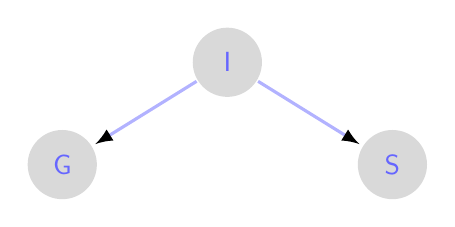
\begin{tikzpicture}[font=\sffamily,node distance=1.5cm,->,>=latex,auto,line width=0.4mm]
	
	\tikzset{node st/.style={state, draw=none,
			fill=gray!30!white,
			text=blue!60!white}}
	
	\node[node st] (I) {I};
	\node[below=2em of I] (dummy) {};
	\node[node st, left=of dummy] (G) {G};
	\node[node st, right=of dummy] (S) {S};  

	
	\draw[every loop,
	auto=right,
	draw=blue!30!white]
	(I) edge[->] node{} (G)
	(I) edge[->] node{} (S);

	\end{tikzpicture}
\end{center}
This encodes our general assumption that\footnote{We say that an event $\alpha$ is independent of event $\beta$ in $P$ with the notation $P \models (\alpha \perp \beta)$. (Def 2.2, pg 23 of book)} $P \models (S \perp G \mid I)$.

\myspace
\p In general, a naive bayes model assumes that instances fall into one of a number of mutually exclusive and exhaustive \textit{classes}, defined as the set of values that the top variable in the graph can take on\footnote{For the intelligence example, the classes are high intelligence and low intelligence.}. The model also includes some number of \textit{features} $X_1, \ldots X_k$, whose values are typically observed. The \green{naive Bayes assumption} is that the features are conditionally independent given the instance's class.

\myspace
\p \blue{Bayesian Networks}. A Bayesian network $\mathcal{B}$ is defined by a network structure together with its set of CPDs. \green{Causal reasoning} (or prediction) refers to computing the downstream effects of various factors (such as intelligence). \green{Evidential reasoning} (or explanation) is the reverse case, where we reason from effects to causes. Finally, \green{intercausal reasoning} (or explaining away) is when different causes of the same effect can interact. For our student example, we could be trying to determine $\Prob{I \mid G}$, the intelligence of an a student given his/her grade in a class. In addition to intelligence being a cause for the grade, we could have another causal variable $D$ for the difficulty of the class:

\begin{center}
	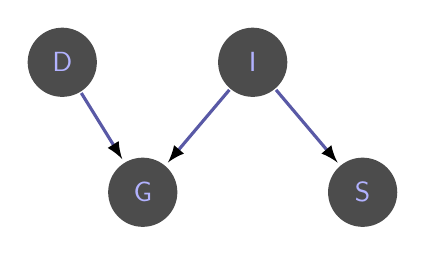
\begin{tikzpicture}[font=\sffamily,node distance=1.5cm,->,>=latex,auto,line width=0.4mm]
	
	\tikzset{node st/.style={state, draw=none,
			fill=gray!60!black,
			text=blue!30!white}}
	
	\node[node st] (I) {I};
	\node[node st, left=of I] (D) {D};
	
	\node[below=3em of I] (dummy) {};
	\node[node st, left=0.8cm of dummy] (G) {G};
	\node[node st, right=0.8cm of dummy] (S) {S};  
	
	\draw[every loop,
		auto=right,
		draw=blue!30!gray]	
	(I) edge[->] node{} (G)
	(I) edge[->] node{} (S)
	(D) edge[->] node{} (G);
	
	\end{tikzpicture}
\end{center}

An example of intercausal reasoning would be observing $D$, so that we now we want $\Prob{I \mid G, d}$; the diffulty of the course can help \textit{explain away} good/bad grades, thus changing our value for the probability of intelligence based on the grade alone. \\

A \green{Bayesian network structure} $\mathcal{G}$ is a DAG whose nodes represent RVs $X_1, \ldots X_n$. Let $Pa_{X_i}^{\mathcal{G}}$ denote the parents of $X_i$ in $\mathcal G$, and $\text{NonDesc}_{X_i}$ denotes the variables that are NOT descendants of $X_i$. Then $\mathcal G$ encodes the following set of \purple{\textit{local independencies}},
	\begin{align}
	\mathcal{I}_{\ell}(\mathcal G) \triangleq \{  \forall X_i : (X_i \perp \text{NonDesc}_{X_i} \mid Pa_{X_i}^{G})  \}
	\end{align}


\myspace
\p \blue{Graphs and Distributions}. Here we see that a distribution $P$ satisfies the local independencies associated with a graph $\mathcal G$ iff $P$ is representable as a set of CPDs associated with $\mathcal G$.  
\begin{compactitem}
	\item \textbf{Local independencies}. Let $P$ be a distribution over $\mathcal{X}$. We define $\mathcal I (P)$ to be the set of \green{independence assertions} of the form $(\matr X \perp \matr Y \mid \matr Z)$ that hold in $P$. The statement ``$P$ satisfies the local independencies associated with $\mathcal G$'' can thus be succinctly written:
	\begin{align}
		\mathcal{I}_{\ell}(\mathcal G) \subseteq \mathcal{I}(P)
	\end{align}
	and we'd say that $\mathcal G$ is an \green{I-map} (independency map) for $P$. 
	
	\item \textbf{I-maps}. More generally, let $\mathcal K$ be \textit{any} graph object associated with a set of independencies $\mathcal I(\mathcal K)$. We say that $\mathcal K$ is an \green{I-map} for a set of independencies $\mathcal I$ if $\mathcal I(\mathcal K) \subseteq \mathcal I$. Note that the complete graph (every two nodes connected) is an I-map for any distribution. 
	
	\item \textbf{Factorization}. Let $\mathcal G$ be a BN graph over $X_1, \ldots, X_n$. We say that a distribution $P$ over the same space \green{factorizes} according to $\mathcal G$ if $P$ can be expressed as 
	\begin{align}
		P(X_1, \ldots, X_n) &= \prod_{i = 1}^n P(X_i \mid Pa_{X_i}^{\mathcal G})
	\end{align}
	For BNs, the following equivalence holds: 
	$$
		\mathcal G \text{ is an I-map for } P \iff P \text{ factorizes according to } \mathcal G
	$$
	
\end{compactitem}

\myspace
\p \blue{D-separation}. We want to understand when we can \textit{guarantee} that an independence $(\matr X \perp \matr Y \mid \matr Z)$ holds in a distribution associated with a BN structure $\mathcal G$. Consider a 3-node network consisting of X, Y, and Z, where X and Y are not directly connected. There are four such cases, which I've drawn below.\marginnote{The fourth trail is called a \textit{v-structure}.}[2em]


\begin{center}
	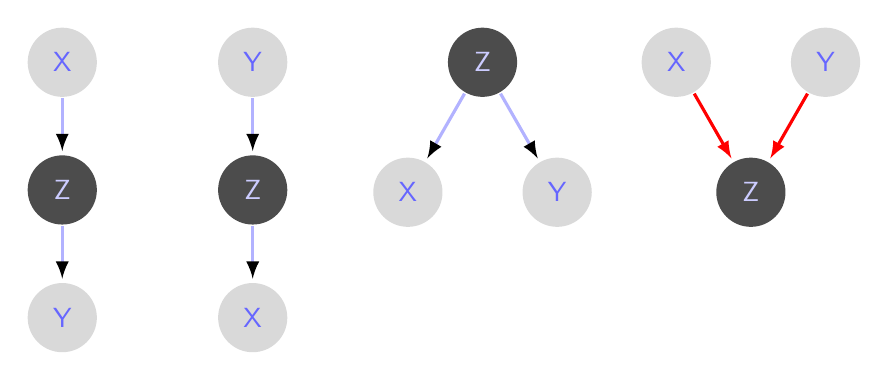
\begin{tikzpicture}[font=\sffamily,node distance=1.5cm,->,>=latex,auto,line width=0.4mm]
	
	\tikzset{node st/.style={state, draw=none,
			fill=gray!30!white,
			text=blue!60!white}}
	\tikzset{node obs/.style={state, draw=none,
			fill=gray!60!black,
			text=blue!20!white}}
	
	\node[node st] (X1) {X};
	\node[node obs, below=2em of X1] (Z1) {Z};
	\node[node st, below=2em of Z1] (Y1) {Y};
	
	
	\node[node st, right=of X1] (X2) {Y};
	\node[node obs, below=2em of X2] (Z2) {Z};
	\node[node st, below=2em of Z2] (Y2) {X};

	
	\node[node obs, right=2cm of X2] (Z3) {Z};
	\node[below=3em of Z3] (dummy1) {};
	\node[node st, left=1em of dummy1] (X3) {X};
	\node[node st, right=1em of dummy1] (Y3) {Y};

	
	\node[right=8em of Z3] (dummy2) {};
	\node[node st, left=1em of dummy2] (X4) {X};
	\node[node st, right=1em of dummy2] (Y4) {Y};
	\node[node obs, below=3em of dummy2] (Z4) {Z};

	
	\draw[every loop,
		auto=right,
		draw=blue!30!white]
	(X1) edge[->] node{} (Z1)
	(Z1) edge[->] node{} (Y1)
	(X2) edge[->] node{} (Z2)
	(Z2) edge[->] node{} (Y2)
	(Z3) edge[->] node{} (X3)
	(Z3) edge[->] node{} (Y3)
	(X4) edge[->, red] node{} (Z4)
	(Y4) edge[->, red] node{} (Z4);	
	\end{tikzpicture}
\end{center}
From left-to-right: indirect causal effect, indirect evidential effect, common cause, common effect. The first 3 satisfy $(X \perp Y \mid Z)$, but the 4th does not. Another way of saying this is that the first 3 trails are \green{active}\footnote{When influence can flow from X to Y via Z, we say that the trail $X \rightleftharpoons Y \rightleftharpoons Z$ is \textit{active}.} IFF $Z$ is not observed, while the 4th trail is active IFF $Z$ (or a descendent of $Z$) is observed. \\

\p \textbf{General case}:
\vspace{-0.5em}
\begin{quote}
	{\itshape Let $\mathcal G$ be a BN structure, and $X \rightleftharpoons \cdots \rightleftharpoons X_n$ a trail in $\mathcal G$. Let $\Z$ be a subset of observed variables. The trail is \green{active} given $\Z$ if 
		\begin{compactitem}
			\item Any v-structure $X_{i - 1} \rightarrow X_i \leftarrow X_{i + 1}$ has $X_i$ or one of its descendants in $\Z$.
			\item No other node along the trail is in $\Z$. 
		\end{compactitem}
	}
\end{quote}

\newcommand{\dsep}{\text{d-sep}_{\mathcal G}}
\p \textbf{D-separation}: (Directed separation)
\vspace{-0.5em}
\begin{quote}
	{\itshape Let $\X$, $\Y$, $\Z$ be three sets of nodes in $\mathcal G$. We say that $\X$ and $\Y$ are \green{d-separated} in $\mathcal G$, denoted $\dsep(\X; \Y \mid \Z)$, if there is no active trail between any node $X \in \X$ and $Y \in \Y$ given $\Z$. We use $\mathcal{I}(\mathcal G)$ to denote the set of independencies that correspond to d-separation,
		\begin{align}
			\mathcal{I}(\mathcal G) &= \{ \mred{\big(}  \X \perp \Y \mid \Z \mred{\big)}  : \dsep(\X ; \Y \mid \Z) \}
		\end{align}
		also called the set of \green{global Markov independencies}.
	}
\end{quote}

\myspace
\p \blue{Soundness and Completeness} of d-separation as a method for determining independence. 
\begin{compactitem}
	\item \textbf{Soundness} (Thm 3.3). If a distribution $P$ factorizes according to $\mathcal G$, then $\mathcal I(\mathcal G) \subseteq \mathcal I(P)$. 
	
	\item \textbf{Completeness}. For any distribution $P$ that factorizes over $\mathcal G$, we have that $P$ is \purple{faithful}\footnote{$P$ is faithful to $\mathcal G$ if, whenever $X \perp Y \mid \Z \in \mathcal{I}(P)$, then $\dsep(X; Y \mid \Z)$.} to $\mathcal G$: 
	\begin{align}
		X \perp Y \mid \Z \in \mathcal{I}(P) ~ \implies ~ \dsep(X; Y \mid \Z)
	\end{align}
\end{compactitem}
To see the detailed algorithm for finding nodes reachable from $X$ given $\Z$ via active trails, see Algorithm 3.1 on pg. 75 of the book.






% ======================================================================================
\lecture{Probabilistic Graphical Models}{Undirected Graphical Models (Ch. 4)}{November 03, 2017}
% ======================================================================================
\vspace{-1.7em}
{\scriptsize Koller and Friedman (2009). Undirected Graphical Models.\\ \textit{Probabilistic Graphical Models: Principles and Techniques}.\\ }


\p \blue{The Misconception Example}. Consider a scenario where we have four students who get together in pairs to work on homework for a class. Only the following pairs meet: (Alice, Bob), (Bob, Charles), (Charles, Debbie), (Debbie, Alice). The professor misspoke in class, giving rise to a possible misconception among the students. We have four binary random variables, $\{A, B, C, D\}$, representing whether the student has the misconception (1) or not (0) \footnote{A student might not have the misconception if e.g. they went home and figured out the problem via reading the textbook instead.}. Intuitively, we want to model a distribution that satisfies $(A \perp C \mid \{B, D\})$, and $(B \perp D \mid \{A, C\})$, but no other independencies\footnote{These independences cannot be naturally captured in a Bayesian (i.e. directed) network.}. Note that the interactions between variables seem symmetric here -- students influence each other (out of the ones they have a pair with). \\

\begin{center}
	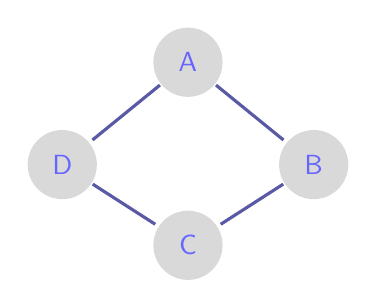
\begin{tikzpicture}[font=\sffamily,node distance=1.cm,->,>=latex,auto,line width=0.4mm]
	
	
	\tikzset{node st/.style={state, draw=none,
			fill=gray!30!white,
			text=blue!60!white}}
	\tikzset{node obs/.style={state, draw=none,
			fill=gray!60!black,
			text=blue!20!white}}
	
	\node[node st] (A) {A};
	\node[below=2em of A] (dummy) {};
	\node[node st, left=of dummy] (D) {D};
	\node[node st, right=of dummy] (B) {B};  
	\node[node st, below=4em of A] (C) {C};
	
	\draw[every loop,
		auto=right,
		draw=blue!30!gray]
	(A) edge[-] node{} (B)
	(A) edge[-] node{} (D)
	(B) edge[-] node{} (C)
	(D) edge[-] node{} (C);
	\end{tikzpicture}
\end{center}

The nodes in the graph of a \green{Markov network} represent the variables, and the edges correspond to a notion of direct probabilistic interaction between the neighboring variables -- an interaction that is not mediated by any other variable in the network. So, how should we parameterize our network? We want to capture the \green{affinities} between the related variables (e.g. Alice and Bob are more likely to agree than disagree).\marginnote{We restrict our attention to nonnegative factors.}[2em]
\begin{quote}
	{\itshape Let $\matr{D}$ be a set of random variables. We define a \green{factor} $\phi$ to be a function from $Val(\matr{D})$ to $\R$. A factor is nonnegative if all its entries are nonnegative. $\matr{D}$ is called the \green{scope} of the factor, denoted $Scope[\phi]$. 
	}
\end{quote}
The factors need not be normalized. Therefore, to interpret probabilities over factors, we must normalize it with what we'll call the \green{partition function}, $Z$:
\begin{align}
	\Prob{a, b, c, d} &= \inv{Z} \phi_1(a, b) \cdot \phi_2(b, c) \cdot \phi_3(c, d) \cdot \phi_4(d, a) \\
	Z &= \sum_{a, b, c, d} \phi_1(a, b) \cdot \phi_2(b, c) \cdot \phi_3(c, d) \cdot \phi_4(d, a)  
\end{align}

\myspace
\p \blue{Parameterization}. Associating the graph structure with a set of parameters. We parameterize undirected graphs by associating a set of factors with it. First, we introduce the definition of \green{factor product}:
\vspace{-0.5em}
\begin{quote}
	{\itshape Let $\matr{X}$, $\matr{Y}$, and $\matr Z$ be three disjoint sets of variables, and let $\phi_1(\matr X, \matr Y)$ and $\phi_2(\matr Y, \matr Z)$ be two factors. We define the \underline{factor product} $\phi_1 \times \phi_2$ to be a factor $\psi: Val(\matr X, \matr Y, \matr Z) \mapsto \R$ as follows:
		\begin{align}
			\psi(\matr X, \matr Y, \matr Z) = \phi_1(\matr X, \matr Y) \cdot \phi_2(\matr Y, \matr Z)
		\end{align}
	}
\end{quote}
We use this to define an undirected parameterization of a distribution:
\vspace{-1em}
\begin{quote}
	{\itshape A distribution $P_{\matr{\Phi}}$ is a \green{Gibbs distribution} parameterized by a set of factors $\matr{\Phi} = \{\phi_1(\matr[1]{D}, \ldots, \phi_K(\matr[K]{D}) )\}$ if it is defined as follows:
		\begin{align}
			P_{\matr{\Phi}} &= \inv{Z} \widetilde{P}_{\matr{\Phi}}(X_1, \ldots, X_n) \\
			 \widetilde{P}_{\matr{\Phi}}(X_1, \ldots, X_n) &= \phi_1(\matr[1]{D}) \times \phi_2(\matr[2]{D}) \times \cdots \times \phi_K(\matr[K]{D})
		\end{align}
	}
\end{quote}
where the authors (Koller and Friedman) have made a point to emphasize: \textbf{A factor is only one contribution to the overall joint distribution. The distribution as a whole has to take into consideration the contributions from all of the factors involved.} Now, we relate the parameterization of a Gibbs distribution to a graph structure.
\vspace{-0.5em}
\begin{quote}
	{\itshape A distribution $P_{\matr{\Phi}}$ with $\matr{\Phi} = \{\phi_1(\matr[1]{D}, \ldots, \phi_K(\matr[K]{D}) )\}$ \green{factorizes} over a Markov network $\mathcal{H}$ if each $\matr[k]{D} (k = 1, \ldots, K)$ is a complete subgraph\footnote{A subgraph is complete if every two nodes in the subgraph are connected by some edge. The set of nodes in such a subgraph is often called a \green{clique}. A clique $\matr{X}$ is maximal if for any superset of nodes $\matr{Y} \supset \matr{X}$, $\matr{Y}$ is \textit{not} a clique.} of $\mathcal{H}$.
	}
\end{quote}
The factors that parameterize a Markov network are often called \green{clique potentials}. Although it can be used without loss of generality, the parameterization using maximal clique potentials generally obscures structure that is present in the original set of factors. Below are some useful definitions that we will use often. \\

\p \textbf{Factor reduction}:
\vspace{-0.5em}
\begin{quote}
	{\itshape Let $\phi(\matr{Y})$ be a factor, and $\matr{U} = \vec{u}$ an assignment for $\matr U \subseteq \matr Y$. Define the \green{reduction} of the factor $\phi$ to the context $\matr U = \vec u$, denoted $\phi[\vec u]$, to be a factor over the scope $\matr{Y}' = \matr Y - \matr U$, such that
		\begin{align}
			\phi[\vec u](\vec{y}') = \phi(\vec{y}', \vec u)
		\end{align}
	For $\matr U \nsubseteq \matr Y$, define $\phi[\vec u]$ only for the assignments in $\vec u$ to the variables in $\matr{U}' = \matr U \cap \matr Y$. 
	}
\end{quote}

\p \textbf{Reduced Gibbs distribution}:
\vspace{-0.5em}
\begin{quote}
	{\itshape Let $P_{\matr{\Phi}}(\matr X)$ be a Gibbs distribution parameterized by $\matr{\Phi} = \{\phi_1, \ldots, \phi_K\}$ and let $\vec u$ be a context. The \green{reduced Gibbs distribution} $P_{\matr{\Phi}}[\vec u]$ is the Gibbs distribution defined by the set of factors $\matr{\Phi}[\vec u] = \{\phi_1[\vec u], \ldots, \phi_K[\vec u] \}$. More formally:
		\begin{align}
			P_{\matr{\Phi}}[\vec u] = P_{\matr{\Phi}}(\matr W \mid \vec u) \quad \text{where} \quad \matr W = \matr X - \matr U
		\end{align}
	}
\end{quote}

\p \textbf{Reduced Markov Network}:
\vspace{-1em}
\begin{quote}
	{\itshape Let $\mathcal H$ be a Markov network over $\matr{X}$ and $\matr{U} = \vec{u}$ a context. The \green{reduced Markov network} $\mathcal{H}[\vec{u}]$ is a Markov network over the nodes $\matr{W} = \matr{X} - \matr{U}$, where we have an edge $X \text{---} Y$ if there's an edge $X \text{---} Y$ in $\mathcal H$. 
	}
\end{quote}
Note that if a Gibbs distribution $P_{\Phi}(\matr{X})$ factorizes over $\mathcal H$, then $P_{\Phi}[\vec u]$ factorizes over $\mathcal{H}[\vec u]$. 

\myspace
\p \blue{Markov Network Independencies}. A formal presentation of the undirected graph as a representation of independence assertions.
\begin{compactitem}
	\item \green{Active Path}. Let $\mathcal H$ be a Markov network structure, and let $X_1 \text{---} \cdots \text{---} X_k$ be a path in $\mathcal H$. Let $\matr{Z} \subseteq \mathcal{X}$ be a set of \textit{observed variables}. The path is \textit{active} given $\matr{Z}$ if none of the $X_i$'s is in $\matr{Z}$. 
	
	\item \green{Separation}. A set of nodes $\matr{Z}$ \textit{separates} $\matr{X}$ and $\matr Y$ in $\mathcal H$, denoted $\text{sep}_{\mathcal H}(\matr X ; \matr Y \mid \matr Z)$, if there is no active path between any node $X \in \matr X$ and $Y \in \matr Y$ given $\matr  Z$. 
	
	\item \green{Global Independencies}. The \textit{global independencies} associated with $\mathcal H$ are defined as
	\begin{align}
		\mathcal{I}(\mathcal H) &= \{  (\matr X \perp \matr Y \mid \matr Z) : \text{sep}_{\mathcal H}(\matr X ; \matr Y \mid \matr Z)  \}
	\end{align}
	This is the \textit{separation criterion}. Note that the definition of separation is monotonic in $\matr{Z}$: if it holds for $\matr{Z}$, then it holds for any $\matr{Z}' \supset \matr{Z}$ as well\footnote{Which means that Markov networks are fundamentally incapable of representing nonmonotonic independence relations!}.
	
	\Needspace{15\baselineskip}
	\item \green{Soundness} of the separation criterion for detecting independence properties in distributions over $\mathcal{H}$. In other words, we want to prove that $$(P \text{ factorizes over }\mathcal{H}) \implies \big[\sep (\matr X ; \matr Y \mid \matr Z) \implies P \models (\matr X \perp \matr Y \mid \matr Z)\big]$$where the portion in brackets can equivalently be said as ``$\mathcal{H}$ is an I-map for $P$''. \\
	\begin{example}[Proof]
	\begin{compactitem}
		\item Consider the case where $\X \cup \Y \cup \Z = \mathcal{X}$. 
		
		\item Then, any clique in $\mathcal{X}$ is fully contained in either $\X \cup \Z$ or $\Y \cup \Z$. In other words,
		\begin{align}
			P(\X, \Y, \Z) &= \inv{Z} f(\X, \Z) g(\Y, \Z) \\
			\text{which implies}\quad
			P(\X, \Y \mid \Z) &= \dfrac{
				f(\X, \Z) g(\Y, \Z)
				}{
				\sum_{x, y} f(x, \Z) g(y, \Z)
				}
		\end{align}
		
		\item We can prove that $P \models (\X \perp \Y \mid \Z)$ by showing that $P(\X, \Y \mid \Z) = P(\X \mid \Z) P(\Y \mid \Z)$. 
		\begin{align}
			P(\X, \Y \mid \Z) &= \frac{f(\X, \Z) g(\Y, \Z)}{P(\Z)} \\
			&=  \frac{f(\X, \Z) g(\Y, \Z)}{P(\Z)} \frac{P(\Z)}{P(\Z)} \\
			&=  \frac{f(\X, \Z) g(\Y, \Z)}{P(\Z)} \frac{ \sum_x f(x, \Z) \sum_y g(y, \Z) }{ P(\Z) } \\
			&=  \frac{f(\X, \Z)  \sum_y g(y, \Z) }{P(\Z)} \frac{ g(\Y, \Z) \sum_x f(x, \Z)}{ P(\Z) } \\
			&= P(\X \mid \Z) P(\Y \mid \Z)
		\end{align} 
		
		\item For the general case where $\X \cup \Y \cup \Z = \mathcal{X}$, let $\matr{U} = \mathcal{X} - (\X \cup \Y \cup \Z )$. Since we know that $\sep (\matr X ; \matr Y \mid \matr Z)$, we can partition $\matr U$ into two disjoint sets $\matr[1]{U}$ and $\matr[2]{U}$ such that $\sep (\matr X \cup \matr[1]{U} ; \matr Y \cup \matr[2]{U}\mid \matr Z)$. Combining the previous result with the decomposition property\footnote{The decomposition property:$$(\X \perp (\Y, \matr{W}) \mid \Z) \implies (\X \perp \Y \mid \Z)$$} give us the desired result that $P \models (\X \perp \Y \mid \Z)$.
	\end{compactitem}
	\end{example}
\end{compactitem}

\myspace
\p \textbf{Pairwise Independencies}:
\vspace{-0.5em}
\begin{quote}
	{\itshape 
		Let $\mathcal H$ be a Markov network. We define the \green{pairwise independencies} assoc. with $\mathcal{H}$:
		\begin{align}
			\mathcal{I}_{p}(\mathcal H) &= \{ \mred{\big(} X \perp Y \mid \mathcal X  - \{X,Y\} \mred{\big)} ~ : ~ X\text{---}Y \notin \mathcal H  \}
		\end{align}
		which just says ``X is indep. of Y given everything else if there's no edge between X and Y.''
	}
\end{quote}

\newcommand\MB{\mathrm{MB}_{\mathcal H}}

\myspace
\p \textbf{Local Independencies}:
\vspace{-0.5em}
\begin{quote}
	{\itshape 
		For a given graph $\mathcal H$, define the \green{Markov blanket} of $X$ in $\mathcal H$, denoted $\MB(X)$, to be the neighbors of $X$ in $\mathcal{H}$. We define the \green{local independencies} associated with $\mathcal H$:
		\begin{align}
			\mathcal{I}_{\ell}(\mathcal H) &= \{ \mred{\big(}X \perp \mathcal X - \{X\}  - \MB(X) \mid \MB(X)  \mred{\big)}  ~ : ~ X \in \mathcal X   \}
		\end{align}
	}
	which just says ``X is indep. of the rest of the nodes in the graph given its immediate neighbors.''
\end{quote}

\myspace
\p \blue{Log-Linear Models}. Certain patterns involving particular values of variables for a given factor can often be more easily seen by converting factors into log-space. More precisely, we can rewrite a factor $\phi(\matr D)$ as
\begin{align}
	\phi(\matr D) &= e^{- \epsilon(\matr D)} \\
	\epsilon(\matr D) &\triangleq -\ln \phi(\matr D) \\
	\Prob{X_1, \ldots, X_n} &\propto e^{- \sum \epsilon_i(\matr[i]{D}   )}
\end{align} 
where $\epsilon(\matr D)$ is often called an \green{energy function}. Note how $\epsilon$ can take on any value along the real line (i.e. removes our nonnegativity constraint)\footnote{We seem to be implicitly assuming that the original factors are all \textit{positive} (not just non-negative).}. Also note that as the $\epsilon$ summation approaches 0, the probability approaches one. 

\myspace\Needspace{10\baselineskip}
This motivates introducing the notion of a \green{feature}, which is just a factor without the nonnegativity requirement. A popular type of feature is the \green{indicator feature} that takes on value 1 for some values $\vec y \in Val(\matr D)$ and 0 otherwise. We can now provide a more general definition for our notion of log-linear models:
\vspace{-0.5em}
\begin{quote}
	{\itshape
	A distribution $P$ is a \green{log-linear model} over a Markov network $\mathcal H$ if it is associated with:
	\begin{compactitem}
		\item A set of features $\mathcal F = \{ f_1(\matr[1]{D}), \ldots, f_k(\matr[k]{D})  \}$ where each $\matr[i]{D}$ is a complete subgraph (i.e. a clique)in $\mathcal H$. 
		\item A set of weights $w_1, \ldots, w_k$. 
	\end{compactitem} 
	such that
	\begin{align}
		\Prob{X_1, \ldots, X_n} &= \inv{Z} \exp \left[ - \sum_{i =1}^{k} w_i f_i(\matr[i]{D})  \right]
	\end{align}
	}
\end{quote}
The log-linear model provides a much more compact representation for many distributions, especially in situations where variables have large domains (such as text).\\
\begin{example}[Box 4.C -- Concept: Ising Models and Boltzmann Machines]
	The \green{Ising model}: Each atom is modeled as a binary RV $X_i \in \{+1, -1\}$ denoting its spin. Each pair of neighboring atoms is associated with energy function $\epsilon_{i,j}(x_i, x_j) = w_{i,j} x_i x_j$. We also have individual energy functions $u_i x_i$ for each atom. This defines our distribution:
	\begin{align}
		P(\xi) = \inv{Z} \exp \bigg( - \sum_{i < j} w_{i,j}x_i x_j - \sum_i u_i x_i   \bigg)
	\end{align}
	
	The \green{Boltzmann distribution}: Now the variables are $X_i \in \{0, 1\}$. The distribution of each $X_i$ given its neighbors is 
	\begin{align}
		P(x_i^1 \mid Nb(X_i)) &= \text{sigmoid}(z) \\
		z &= -(\sum_j w_{i,j} x_j  )-u_i
	\end{align}
\end{example}

\begin{example}[Box 4.D -- Concept: Metric MRFs]
	Consider the pairwise graph $X_1,\ldots, X_n$ in the context of sequence labeling. We want to assign each $X_i$ a label. We also want adjacent nodes to prefer being similar to each other. We usually use the MAP objective, so our goal will be to minimize the total energy over the parameters (which are given by the individual energy functions $\epsilon_i$).
	\begin{align}
		E(x_1, \ldots, x_n) &= \sum_i \epsilon_i (x_i) + \sum_{(i,j) \in \mathcal{E}} \epsilon_{i,j}(x_i, x_j)
	\end{align}
	The simplest place to start for preferring neighboring labels to take on similar values is to define $\epsilon_{i,j}$ to have low energy when $x_i = x_j$ and some positive $\lambda_{i,j}$ otherwise. We want to have finer granularity for our similarities between labels. To do this, we introduce the definition of a \green{metric}: a function $\mu : \mathcal V \times \mathcal V \mapsto [0, \infty)$ that satisfies
	\begin{align}
		\green{\text{[reflexivity]}}&  \qquad \mu(v_k, v_l) = 0 \quad \text{IFF} \quad k = l \\
		\green{\text{[symmetry]}}& \qquad \mu(v_k, v_l) = \mu(v_l, v_k) \\
		\green{\text{[triangle inequality]}}& \qquad \mu(v_k, v_l) + \mu(v_l, v_m) \ge \mu(v_k, v_m)
	\end{align}
	and we can now let $\epsilon_{i,j}(v_k, v_l) := \mu(v_k, v_l)$. 
\end{example}

\myspace
\p \blue{Canonical Parameterization} (4.4.2.1). Markov networks are generally overparameterized\footnote{Meaning: for any $P_{\Phi}$, there are often infinitely many ways to choose its set of parameter values for a given $\mathcal H$.}. The \green{canonical parameterization}, \underline{which requires that $P$ be positive}, avoids this. First, some notation and requirements:
\begin{compactitem}
	\item P must be positive. 
	\item Let $\xi^* = (x_1^*, \ldots, x_n^*)$ denote some fixed assignment to the network variables $\mathcal X$. 
	\item Define $\vec[\Z]{x} \triangleq \vec{x}\langle \Z \rangle$ as the assignment of variables in some subset $\Z$.\footnote{And $\vec x$ is some assignment to some subset of $\mathcal X$ that also contains $\Z$.}
	\item Define $\xi^*_{-\Z} \triangleq \xi^*\langle \mathcal X - \Z \rangle$ be our fixed assignment for the variables outside $\matr Z$. 
	\item Let $\ell(\xi)$ denote $\ln P(\xi)$.  
\end{compactitem}

\Needspace{10\baselineskip}
The \green{canonical energy function} for a clique $\matr D$ is defined below, as well as the associated total $P(\xi)$ over a full network assignment:\marginnote{The sum is over all subsets of $\matr D$, including $\matr D$ itself and $\varnothing$.}[1em]
\graybox{
	\epsilon^*_{\matr D}(\vec d) &= \sum_{\Z \subseteq \matr D} \ell(\vec[\Z]{d}, \xi^*_{-\Z}) \cdot (-1)^{|\matr D - \Z|} \\
	P(\xi) &= \exp\bigg[ \sum_i \epsilon^*_{\matr[i]{D}}(  \xi\langle \matr[i]{D} \rangle )     \bigg] \label{thm-4.7}
}


\myspace
\p \blue{Conditional Random Fields}. So far, we've only described Markov network representation as encoding a joint distribution over $\mathcal X$. The same undirected graph representation and parameterization can also be used to encode a \textit{conditional distribution} $\Prob{\matr Y \mid \matr X}$, where $\matr Y$ is a set of \textit{target variables} and $\matr X$ is a (disjoint) set of \textit{observed variables}.\marginnote{Note how there are no connection between any of the $X$s}[4em]
\begin{center}
	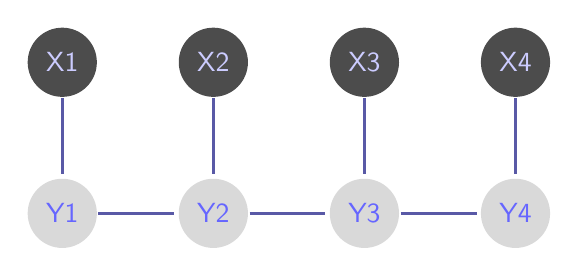
\begin{tikzpicture}[font=\sffamily,node distance=1.cm,->,>=latex,auto,line width=0.4mm]
		
		\tikzset{node st/.style={state, draw=none,
				fill=gray!30!white,
				text=blue!60!white}}
		\tikzset{node obs/.style={state, draw=none,
				fill=gray!60!black,
				text=blue!20!white}}
	
	\node[node obs] (X1) {X1};
	\node[node obs, right=of X1] (X2) {X2};
	\node[node obs, right=of X2] (X3) {X3};
	\node[node obs, right=of X3] (X4) {X4};

	\node[node st, below=of X1] (Y1) {Y1};
	\node[node st, right=of Y1] (Y2) {Y2};
	\node[node st, right=of Y2] (Y3) {Y3};
	\node[node st, right=of Y3] (Y4) {Y4};
	
	\draw[every loop,
		auto=right,
		draw=blue!30!gray]
	(X1) edge[-]				node{} (Y1)
	(X2) edge[-]				node{} (Y2)
	(X3) edge[-]				node{} (Y3)
	(X4) edge[-]				node{} (Y4)
	(Y1) edge[-] 				node{} (Y2)
	(Y2) edge[-] 				node{} (Y3)
	(Y3) edge[-] 				node{} (Y4);
	\end{tikzpicture}
\end{center}

\p Formally, a CRF is an undirected graph $\mathcal H$ whose nodes correspond to $\matr Y \cup \matr X$. Since we want to avoid representing\footnote{Also note how we never have to deal with a summation over all possible $\X$, due to restricting ourselves to $Z(\X)$.} a probabilistic model over $\matr X$, we disallow potentials that involve only variables in $\matr X$; our set of factors is $\phi_1(\matr[1]{D}), \ldots, \phi_m(\matr[m]{D})$, such that each $\matr[i]{D} \nsubseteq \matr{X}$. The network encodes a conditional distribution as follows:
\graybox{
	P(\Y \mid \X) &= \inv{Z(\X)} \widetilde{P}(\Y, \X)	\\
	 \widetilde{P}(\Y, \X) &= \prod_{i = 1}^{m} \phi_i(\matr[i]{D}) \\
	 Z(\matr X) &= \sum_{\matr Y}  \widetilde{P}(\matr Y, \X)
}
where now the partition function is a function of the assignment $\vec x$ to $\matr X$. 

\myspace
\p \blue{Rapid Summary}. 
\begin{compactitem}
	\item \textbf{Gibbs distribution}: any probability distribution that can be written as a product of factors divided by some partition function $Z$. 
	\item \textbf{Factorizes}: A Gibbs distribution factorizes over $\mathcal H$ if each factor [in its product of factors] is a clique. 
\end{compactitem}

\myspace
\subsub{Exercises}
\myspace

%\tikzstyle{gnode}=[state, fill=gray!60!black, text=blue!30!white, draw=none]
%\tikzstyle{myedge}=[-, orange]

\begin{example}[Exercise 4.1]
	\textit{Let $\mathcal{H}$ be the graph of binary variables below. Show that P does not factorize over $\mathcal{H}$ (Hint: proof by contradiction).}
	\begin{center}
		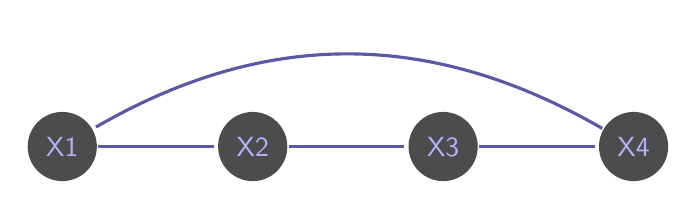
\begin{tikzpicture}[font=\sffamily,node distance=1.5cm,->,>=latex,auto,line width=0.4mm]
		
		\tikzset{node st/.style={state, draw=none,
								fill=gray!60!black,
								text=blue!30!white}}
		
		\node[node st] (X1) {X1};
		\node[node st, right=of X1] (X2) {X2};
		\node[node st, right=of X2] (X3) {X3};
		\node[node st, right=of X3] (X4) {X4};
		
		\draw[every loop,
			  auto=right,
			  draw=blue!30!gray]
		(X1) edge[-] 				node{} (X2)
		(X2) edge[-] 				node{} (X3)
		(X3) edge[-] 				node{} (X4)		
		(X4) edge[-, bend right] 	node{} (X1);				
		\end{tikzpicture}
	\end{center}
	\begin{compactitem}
		\item Example 4.4 recap: P satisfies the global independencies w.r.t $\mathcal{H}$. They showed this by manually checking the two global indeps of $\mathcal{H}$, $(X_1 \perp X_3 \mid X_2, X_4)$ and $(X_2 \perp X_4 \mid X_1, X_3)$, against the tabulated list of possible assignments for $P$ (given in example). Nothing fancy. 
		\item P factorizes over $\mathcal{H}$ if it can be written as a product of clique potentials.
		\item My proof:
		\begin{compactenum}
			\item Assume that $P$ \textit{does} factorize over $\mathcal{H}$.
			\item Then $P$ can be written as
			\begin{align}
				P(X_1, X_2, X_3, X_4) &= \inv{Z} \phi_1(X_1, X_2) \phi_2(X_2, X_3) \phi_3(X_3, X_4) \phi_4(X_4, X_1)
			\end{align}
			
			Let the above assertion be denoted as $C$, and the statement that $P$ factorizes according to $\mathcal{H}$ be denoted simply as $P_{\mathcal H}$. Since $P_{\mathcal H} \iff C$, if we can prove that $C$ does not hold, then we've found our contradiction, meaning $P_{\mathcal{H}}$ also must not hold.
			
			\item I know that the proof must take advantage of the fact that we know $P$ is zero for certain assignments to $\mathcal{X}$. For example $P(0100) = 0$. Furthermore, by looking at the assignments where $P$ is \textit{not} zero, I can see that all possible combinations of $(X_1, X_2)$ are present, which means $\phi_1$ never evaluates to zero.
			
			\item From the example, we know that $P(1100) = 1/8 \ne 0$. However, since
			\begin{align}
				0 = \frac{P(0100)}{P(1100)} &= \frac{\phi_1(0, 1)\phi_4(0, 0)}{\phi_1(1, 1)\phi_4(0, 1)} \\
			   &= \frac{\phi_4(0, 0)}{\phi_4(0, 1)} \qquad \mred{(\phi_1 > 0)} \label{idkhi}
			\end{align}
			and we also know that both the numerator and denominator of eq. \ref{idkhi} are positive, and thus we have a contradiction. 
		\end{compactenum}
	\end{compactitem}
\end{example}

\begin{comment}
\myspace
\p \blue{Exercise 4.2}. Show that for any constants $\lambda^1$ and $\lambda^0$, and 
\begin{align}
	\epsilon'_1(a, b^i) &:= \epsilon_1(a, b^i) + \lambda^i \\
	\epsilon'_2(b^i, c) &:= \epsilon_2(b^i, c) - \lambda^i
\end{align}
that the $\epsilon'_1$ and $\epsilon'_2$ result in equivalent distributions as the originals. Since we'll be using the misconception network for the next few problems, I've redrawn it below for convenience. 
\begin{center}
	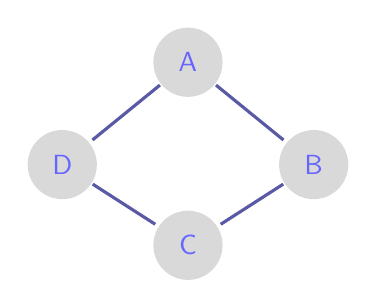
\begin{tikzpicture}[font=\sffamily,node distance=1.cm,->,>=latex,auto,line width=0.4mm]
	
	
	\tikzset{node st/.style={state, draw=none,
			fill=gray!30!white,
			text=blue!60!white}}
	\tikzset{node obs/.style={state, draw=none,
			fill=gray!60!black,
			text=blue!20!white}}
	
	\node[node st] (A) {A};
	\node[below=2em of A] (dummy) {};
	\node[node st, left=of dummy] (D) {D};
	\node[node st, right=of dummy] (B) {B};  
	\node[node st, below=4em of A] (C) {C};
	
	\draw[every loop,
	auto=right,
	draw=blue!30!gray]
	(A) edge[-] node{} (B)
	(A) edge[-] node{} (D)
	(B) edge[-] node{} (C)
	(D) edge[-] node{} (C);
	\end{tikzpicture}
\end{center}
\end{comment}

\begin{example}[Exercise 4.4]
\textit{Prove theorem 4.7 for the case where $\mathcal H$ consists of a single clique.} Theorem 4.7 is equation \ref{thm-4.7} in my notes. For a single clique $\matr D$, the question reduces to: Show that, for any assignment $\vec d$ to $\matr D$:
\begin{align}
	P(\vec d)
	&=  \frac{\exp\bigg( -\epsilon(\vec d)   \bigg)   }{   \sum_{\vec{d}'} \exp\bigg( -\epsilon(\vec{d}')   \bigg)   }    \\
	&= \exp\bigg( \epsilon^*_{\matr D} ( \vec d )  \bigg)
\end{align}

Consider the case where $|\matr D|= 1$, i.e. $\vec d = d$ is a single variable. Then
\begin{align}
	\epsilon^*_{\matr D}(\vec d) 
	&= (-1)^{|\matr D|} \ell(\xi^*_{\matr D}) + (-1)^{|\matr D - \matr D|}\ell(\vec d) \\
	&= -\ell(\xi^*_{\matr D}) + \ell(\vec d) \\
	&= -\ln P(d^*) + \ln P(d)
\end{align}
and therefore
\begin{align}
	 \exp\bigg( \epsilon^*_{\matr D} ( \vec d )  \bigg)
	 &= P(d) / P(d^*)
\end{align}
which is clearly incorrect (???) \red{TODO}: figure out what's going on here. Either the book has a type in its for theorem 4.7, or I'm absolutely insane. 
\end{example}




% ======================================================================================
\lecture{Probabilistic Graphical Models}{Local Probabilistic Models (Ch. 5)}{May 27, 2018}
% ======================================================================================
\vspace{-1.7em}
{\scriptsize Koller and Friedman (2009). Local Probabilistic Models.\\ \textit{Probabilistic Graphical Models: Principles and Techniques}.\\ }

\p \blue{Deterministic CPDs}. When $X$ is a deterministic fu nction of its parents $Pa_X$:
\begin{align}
	P(x \mid Pa_X) = \begin{cases}
		1 & x = f(Pa_X) \\
		0 & \text{otherwise.}
	\end{cases}
\end{align}
Consider the example below, where the double-line notation on C means that C is a deterministic function of A and B. What new conditional dependencies do we have?

\begin{center}
	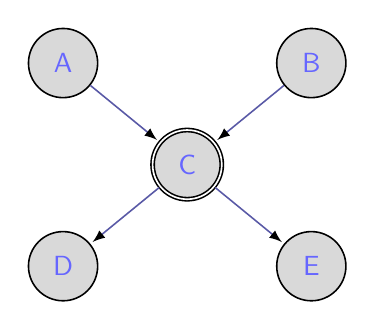
\begin{tikzpicture}[font=\sffamily,node distance=1.cm,->,>=latex,auto,line width=0.2mm]
	
	\tikzset{node st/.style={state,
			fill=gray!30!white,
			text=blue!60!white}}
	\tikzset{node obs/.style={state, draw=none,
			fill=gray!60!black,
			text=blue!20!white}}
	
	\node[node st, accepting] (C) {C};
	\node[above=2em of C] (dumtop) {};
	\node[node st, left=of dumtop] (A) {A};
	\node[node st, right=of dumtop] (B) {B};
	\node[below=2em of C] (dumbot) {};
	\node[node st, left=of dumbot] (D) {D};
	\node[node st, right=of dumbot] (E) {E};
	
	\draw[every loop,
	auto=right,
	draw=blue!30!gray]
	(A) edge [->] node{} (C)
	(B) edge [->] node{} (C)
	(C) edge [->] node{} (D)
	(C) edge [->] node{} (E);	
	\end{tikzpicture}
\end{center}
Answer: $(D \perp E \mid A, B)$, which would not be true by d-separation alone. It only holds because C is a deterministic function of A and B. z




% ======================================================================================
\lecture{Probabilistic Graphical Models}{Template-Based Representations (Ch. 6)}{May 27, 2018}
% ======================================================================================
\vspace{-1.7em}
{\scriptsize Koller and Friedman (2009). Template-Based Representations.\\ \textit{Probabilistic Graphical Models: Principles and Techniques}.\\ }

In what follows, we will build on an example where a vehicle tries to track its true location (L) using various sensor readings: velocity (V), weather (W), failure of sensor (F), observed location (O) of the noisy sensor.
\begin{center}
	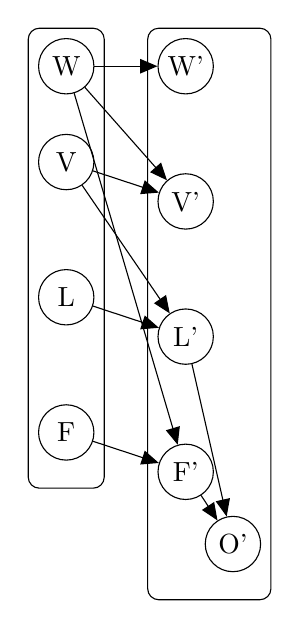
\begin{tikzpicture}[font=\sffamily]
	
	
	% t = 0
	\node[latent] (W) {W};
	\node[latent, below=0.5cm of W] (V) {V};
	\node[latent, below=of V] (L) {L};
	\node[latent, below=of L] (F) {F};
	
	% t = 1
	\node[latent, right=0.8cm of W] (W') {W'};
	\node[latent, below=of W'] (V') {V'};
	\node[latent, below=of V'] (L') {L'};
	\node[latent, below=of L'] (F') {F'};
	\node[latent, below=0.2cm of F', xshift=0.6cm] (O') {O'};
	
	\edge{W} {W',V',F'};
	\edge{V} {V',L'};
	\edge{L} {L'};
	\edge{F} {F'};
	\edge{L',F'} {O'};
	
	\plate {p} 	{(W)(V)(L)(F)} {} ;
	\plate {p2} {(W')(V')(L')(F')(O')} {};
	
	\end{tikzpicture}
\end{center}


\p \blue{Temporal Models}. We discretize time into slices of interval $\Delta$, and denote the ground random variables at time $t \cdot \Delta$ by $\mathcal{X}^{(t)}$. We can simplify our formulation considerably by assuming a \green{Markovian system}: a dynamic system over template variables $\mathcal X$ that satisfies the Markov assumption:
\begin{align}
	(\mathcal{X}^{(t + 1)} \perp \mathcal{X}^{(0:(t-1))} \mid \mathcal{X}^{(t)}) \label{markovian-assumption}
\end{align}
which allows us to define a more compact representation of the joint distribution from time 0 to T:
\begin{align}
	P(\mathcal{X}^{(0:T)}) &= P(\mathcal{X}^{(0)}) \prod_{t = 0}^{T - 1} P(\mathcal{X}^{(t + 1)}  \mid \mathcal{X}^{(t)} ) 
\end{align}
One last simplifying assumption, to avoid having unique transition probabilities for each time $t$, is to assume a \green{stationary}\footnote{Also called time invariant or homogeneous.} Markovian dynamic system, defined s.t. $P(\mathcal{X}^{(t + 1)} \mid \mathcal{X}^{(t)})$ is the same for all $t$.



\myspace
\p \blue{Dynamic Bayesian Networks} (6.2.2). Above, I've drawn the \green{2-time-slice Bayesian network} (2-TBN) for our location example. A 2-TBN is a conditional BN over $\mathcal{X}'$ given $\mathcal{X}_I$, where $\mathcal{X}_I \subseteq \mathcal{X}$ is a set of \purple{interface variables}\footnote{Interface variables are those variables whose values at time $t$ can have a direct effect on the variables at time $t+1$.}. For each template variable $X_i$, the CPD $P(X'_i \mid Pa_{X_i'})$ is a \green{template factor}. We can use the notion of the 2-TBN to define the more general \green{dynamic Bayesian network}:
\begin{definition}
	A \textbf{dynamic Bayesian network} (DBN) is a pair $\langle \beta_0, \beta_{\rightarrow} \rangle$, where $\beta_0$ is a Bayesian network over $\mathcal{X}^{(0)}$, representing the initial distribution over states, and $\beta_{\rightarrow}$ is a 2-TBN for the process. For any $T \ge 0$, the unrolled Bayesian network is defined such that
	\begin{compactitem}
		\item $p(X_i^{(0)} \mid Pa_{X_i^{(0)}})$ is the same as the CPD for the corresponding $X_i$ in $\beta_0$.
		\item $p(X_i^{(t)} \mid Pa_{X_i^{(t)}})$ (for $t > 0$) is the same as the CPD for the corresponding $X_i'$ in $\beta_{\rightarrow}$.  
	\end{compactitem}
\end{definition}

\myspace
\p \blue{State-Observation Models} (6.2.3). Temporal models that, in addition to the Markov assumption (eq. \ref{markovian-assumption}), model the observation variables at time $t$ as conditionally independent of the entire state sequence given the variables at time $t$:
\begin{align}
	\left( 
		\matr{O}^{(t)} \perp \X^{(0:(t-1))}, \X^{(t+1:\infty)}
		\mid
		\X^{(t)}
	\right)
\end{align}
So basically a 2-TBN with the constraint that observation variables are leaves and only have parents in $\X'$. We now view our probabilistic model as consisting of 2 components: the \textit{transition model} $P(\X' \mid \X)$, and the \textit{observation model} $P(\matr O \mid \X)$. The two main architectures for such models are as follows:
\begin{compactitem}
	\item \green{Hidden Markov Models}. Defined as having a single state variable $S$ and a single observation variable $O$. In practice, the transition model $P(S' \mid S)$ is often assumed to be sparse (many possible transitions having zero probability). In such cases, one usually represents them visually as \purple{probabilistic finite-state automaton}\footnote{FSA use the graphical notation where the nodes are the individual possible values in $Val(S)$, and the directed edges from some $a$ \textit{to} $b$ have weight equal to $P(S'=b \mid S=a)$.}.
	
	\item \green{Linear Dynamical Systems} (LDS) represent a system of one or more real-valued variables that evolve linearly over time, with some Gaussian noise. Such systems are often called \purple{Kalman filters}, after the algorithm used to perform tracking. They can be viewed as a DBN with continuous variables and all dependencies are linear Gaussian\footnote{Linear Gaussian: some var $Z$ pointing to $X$ denotes that $X = \Lambda Z + \text{noise}$, where $\text{noise} \sim \mathcal{N}(\mu_x, \Sigma_x)$.}. A LDS is traditionally represented as a state-observation model, where both state and observation are vector-valued RVs, and the transition/observation models are encoded using matrices. More formally, for $\X^{(t)} \in \R^n, O \in \R^m$:\marginnote{
	$$ Q \in \R^{n \times n} $$ $$ H \in \R^{m \times m} $$}[2em]
	\begin{align}
		P(\X^{(t)} \mid \X^{(t-1)})
			&= \mathcal{N}(A \X^{(t-1)}; Q) \\
		P(O^{(t)} \mid \X^{(t)}) 
			&= \mathcal{N}(H \X^{(t)}; R)
	\end{align}
\end{compactitem}

\myspace
\p \blue{Template Variables and Template Factors} (6.3). It's convenient to view the world as being composed of a set of \green{objects}, which can be divided into a set of mutually exclusive and exhaustive \textit{classes} $\mathcal Q = Q_1, \ldots, Q_k$. Template \green{attributes} have a tuple of \textit{arguments}, each of which is associated with a particular class of objects, which defines the set of objects that can be used to instantiate the argument in a given domain. Template attributes thus provide us with a ``generator'' for RVs in a given probability space. Formally,
\begin{definition}
		An \green{attribute} $A$ is a function $A(U_1, \ldots, U_k)$, whose range is some set $Val(A)$, and where each argument $U_i$ is a typed \green{logical variable} associated with a particular class $Q[U_i]$. The tuple $U_1, ldots, U_k$ is called the \green{argument signature} of the attribute $A$, and denoted $\alpha(A)$. 
\end{definition}

\myspace
\p \blue{Plate Models} (6.4.1). The simplest example of a plate model is shown below. It describes multiple RVs generated from the same distribution $\mathcal D$. 

\begin{center}
	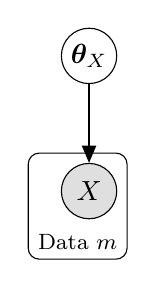
\begin{tikzpicture}[font=\sffamily]
	\node[latent] (theta) {$\vec[X]{\theta}$};
	\node[obs, below=of theta] (X) {$X$};
	
	\edge{theta} {X};
	
	\plate {p} {(X)} {Data $m$} ;
	
	\end{tikzpicture}
\end{center}

This could be a plate model for a set of coin tosses sampled from a single coin. We have a set of $m$ random variables $X(d)$, where $d \in \mathcal D$. Each $X(d)$ is the random variable for the $d$th coin toss. We also explicitly model that the single coin for which the tosses are used is sampled from a distribution $\theta_X$, which takes on values $[0, 1]$ and denotes the bias of the coin. 








% ======================================================================================
\lecture{Probabilistic Graphical Models}{Gaussian Network Models (Ch. 7)}{July 26, 2018}
% ======================================================================================
\vspace{-1.7em}
{\scriptsize Koller and Friedman (2009). Gaussian Network Models.\\ \textit{Probabilistic Graphical Models: Principles and Techniques}.\\ }

\p \blue{Multivariate Gaussians}. Here I'll give two forms of the familiar density function, followed by some comments and terminology.
\begin{align}
	p(\vec x) 
		&= \inv{(2\pi)^{n/2} \sqrt{\det \Sigma}}
			\exp\left\{ 
				-\onehalf (\vec x - \vec\mu)^T \Sigma^{-1} (\vec x - \vec\mu)
			\right\} \\
	p(\vec x) 
		&\propto \exp\left\{ - \onehalf \vec{x}^T J \vec x + (J \vec\mu)^T \vec x  \right\}
		\quad \text{where } J \triangleq \Sigma^{-1}
\end{align}
\begin{compactitem}
	\item The \green{standard Gaussian} is defined as $\mathcal{N}(\vec 0, \matr I)$.
	
	\item $\Sigma$ must be \textit{positive definite}\footnote{Most definitions of p.d. also require that the matrix be symmetric. I also think it helps to view positive definite from the operator perspective: \textit{A linear operator $T$ is positive definite if $T$ is self-adjoint and $\langle T(x), x \rangle > 0$. In other words, ``positive definite'' means that the result of applying the matrix/operator to any nonzero $\vec x$ will always have a positive component along the original direction $\hat{\vec x}$. }}: $\forall \vec x \ne 0, ~ \vec{x}^T \Sigma \vec x > 0$. Recall that $\Sigma_{i,j} = \text{Cov}\left[ x_i, x_j \right] = \E{x_i x_j} - \mu_i \mu_j$.
\end{compactitem}
The two operations we usually want to perform on a Gaussian are (1) computing marginals, and (2) conditioning the distribution on an assignment of some subset of the variables. For (1), its easier to use the standard form of $p(\vec x)$, whereas for (2) it is easier to use the information form (the one using $J$). \\

Multivariate Gaussians are also special because we can easily determine whether two $x_i$ and $x_j$ are independent: $x_i \perp x_j \text{  IFF  } \Sigma_{i,j}=0$\footnote{This is not true in general -- just for multivariate Gaussians!}. For conditional independencies, the information matrix $J$ is easier to work with: $(x_i \perp x_j \mid \{x\}_{k \notin \{i,j\}}) \text{  IFF  } J_{i,j}=0$. This condition is also how we defined pairwise independencies in a Markov network, which leads to the awesome realization:
\begin{definition}
	We can view the information matrix $J$ as directly defining a minimal I-map Markov network for [multivariate Gaussian] $p$, whereby any entry $J_{i,j} \ne 0$ corresponds to an edge $x_i \text{---} x_j$ in the network.
\end{definition}



% ======================================================================================
\lecture{Probabilistic Graphical Models}{Variable Elimination (Ch. 9)}{May 06, 2018}
% ======================================================================================
\vspace{-1.7em}
{\scriptsize Koller and Friedman (2009). Variable Elimination.\\ \textit{Probabilistic Graphical Models: Principles and Techniques}.\\ }

\p \blue{Analysis of Exact Inference}. The focus of this chapter is the conditional probability query,
\begin{align}
	\Prob{\matr Y \mid \matr E = \vec e}
	&= \frac{  \Prob{\matr Y, \vec e}  }{ \Prob{\vec e}  } \tlab{9.1}
\end{align}
Ideally, we want to obtain all instantiations $\Prob{\vec y \mid \vec e}$ of equation \ref{9.1}. Let $\matr W = \mathcal{X} - \matr Y - \matr E$ be the RVs that are neither query nor evidence. Then
\begin{align}
	\Prob{\vec y \mid \vec e} 
	&= \frac { \sum_{\vec w} \Prob{\vec y, \vec e, \vec w}  }{ \sum_{\vec y}  \Prob{\vec y, \vec e} } \tlab{9.3}
\end{align}
and note that, by computing all instantiations for the numerator first, we can reuse them to obtain the denominator. We can formulate the inference problem as a decision problem, which we will call $BNPrDP$, defined as follows\marginnote{$BNPrDP$}[4em]:
\vspace{-0.5em}
\begin{center}
	{\itshape 
	Given: Bayesian network $\mathcal B$ over $\mathcal X$, a variable $X \in \mathcal{X}$, and a value $x \in Val(X)$. \\
	Decide: whether $\Prob[\mathcal B]{X = x} > 0$. 
	}
\end{center}
\purple{Thm 9.1}: The decision problem $BNPrDP$ is $\mathcal{N}\mathcal{P}$-complete. \textbf{Proof}:
\begin{footnotesize}
	\begin{compactenum}
		\item \textbf{BNPrDP is in $\NP$}: Guess a full assignment $\xi$ to the network\footnote{Apparently the time it takes to generate a guess is irrelevant.}. If the guess is successful, where sucess if defined as $(X=x) \in \xi$ and $P(\xi) > 0$, then we know that $P(X=x) > 0$\footnote{This is true because $P(x)$ can be decomposed as $P(\xi) + \sum P(\ldots) \ge P(\xi)$.}. Computing $P(\xi)$ is linear in the number of factors for a BN, since we just multiply them together.
		
		\item \textbf{BNPrDP is $\NP$-hard}. We show this by proving that we can solve 3-SAT (which is $\NP$-hard) by transforming inputs to 3-SAT to inputs of BNPrDP in polynomial time. Given any 3-SAT formula $\phi$, we can create a BN $B_{\phi}$ with some special variable $X$ s.t. $\phi$ is satisfiable IFF $P_{B_{\phi}}(X = x^1) > 0$. You can easily build such a network by having a node $Q_i$ for each binary RV $q_i$, and a node $C_i$ for each of the clauses that's a deterministic function of its parents (up to 3 Q nodes). Then, the node X is a deterministic function of its parents, which are chains of AND gates along the $C_i$. Since each node has at most 3 parents, we can ensure that construction is bounded by polynomial time in the length of $\phi$. 
	\end{compactenum}
\end{footnotesize}

\myspace
\p \blue{Analysis of Approximate Inference}. Consider a specific query $P(\vec y \mid \vec e)$, where we focus on a particular assignment $\vec y$. Let $\rho$ denote some approximate answer, whose accuracy we wish to evaluate relative to the correct probability. We can use the \purple{relative error} to estimate the quality of the approximation: \textit{An estimate $\rho$ has relative error $\epsilon$ if:}
\begin{align}
	\frac{\rho}{1 + \epsilon} \le P(\vec y \mid \vec e) \le \rho (1 + \epsilon)
\end{align}
Unfortunately, the task of finding some approximation $\rho$ with relative error $\epsilon$ \textit{is also $\NP$-hard}. Furthermore, even if we relax this metric by using absolute error instead, we end up finding that \textbf{in the case where we have evidence, approximate inference is no easier than exact inference, in the worst case}.

\myspace
\p \blue{Variable Elimination}. Basically, a dynamic programming approach for performing exact inference. Consider the simple BN $X_1 \rightarrow \cdots \rightarrow X_n$, where each variable can take on $k$ possible values. The dynamic programming approach for computing $P(X_{n})$ involves computing
\begin{align}
	P(X_{i + 1}) = \sum_{x_i} P(X_{i + 1} \mid x_i) P(x_i)
\end{align} 
$n - 1$ times, starting with $i = 1$, all the way up to $i = n - 1$, reusing the previous computation at each step, with total cost $\mathcal{O}(nk^2)$. So for this simple network, even though the size of the joint is $k^n$ (exponential in $n$), we can do inference in linear time. 

First, we formalize some basic concepts before defining the algorithm. 

\p \textbf{Factor marginalization}:
\vspace{-1em}
\begin{quote}
	{\itshape
		Let $\matr X$ be a set of variables, and $Y \notin \matr X$ a variable. Let $\phi(\matr X, Y)$ be a factor. Define the \green{factor marginalization} of $Y$ in $\phi$, denoted $\sum_Y \phi$, to be a factor $\psi$ over $\matr X$ such that:
		$$
		\psi(\matr X) = \sum_Y \phi(\matr X, Y)
		$$	
	}
\end{quote} 
The key observation that's easy to miss is that \textit{we're only summing entries in the table where the values of $\X$ match up}. One useful rule for exchanging factor product and summation: If $X \notin Scope[\phi_1]$, then
\begin{align}
	\sum_X (\phi_1 \cdot \phi_2) = \phi_1 \cdot \sum_X \phi_2 \tlab{9.6}
\end{align}

\Needspace{10\baselineskip}
So, when computing some marginal probability, the main idea is to group factors together and compute expressions of the form
\graybox{
	\sum_{\Z} \prod_{\phi \in \Phi} \phi
} where $\Phi$ is the set of all factors $\phi$ for which $\Z \in Scope[\phi]$. This is commonly called the \green{sum-product} inference task. The full algorithm for sum-product variable elimination, which is an instantiation of the sum-product inference task, is illustrated below.

\myfig[0.4\textwidth]{figs/variable_elimination.png}

This is what we use to compute the marginal probability $P(\X)$ where $\X = \mathcal{X} - \Z$. To compute conditional queries of the form $P(\Y \mid \matr{E} = \vec e)$, simply replace all factors whose scope overlaps with $\matr E$ with their reduced factor (see chapter 4 notes for definition) to get the unnormalized $\phi^*(\Y)$ (the numerator of $P(\Y \mid \vec e)$). Then divide by $\sum_{\vec y} \phi^*$ to obtain the final result.


\myspace
\p \blue{Example}. We will work through computing $P(Job)$ for the BN below. 

\begin{center}
	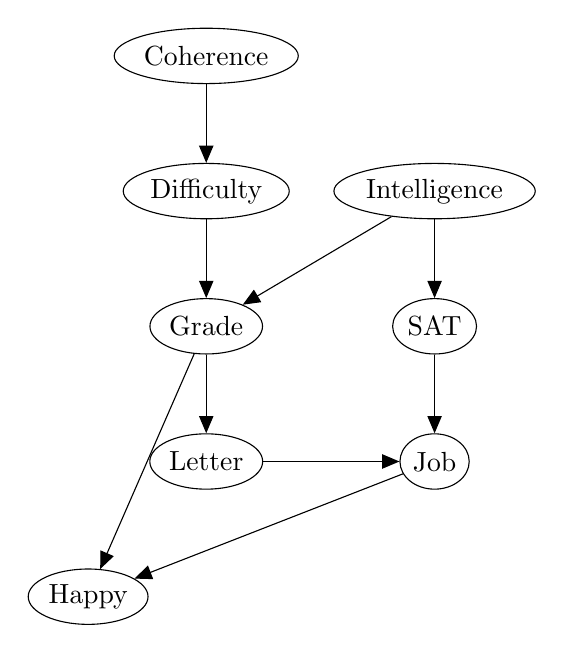
\begin{tikzpicture}[font=\sffamily]
	
	\node[latent, ellipse] (C) 								{Coherence};
	\node[latent, ellipse, below=of C] (D) 					{Difficulty};
	\node[latent, ellipse, below=of C, xshift=2.9cm] (I)	{Intelligence};
	
	\node[latent, ellipse, below=of D] (G) 	{Grade}; 
	\node[latent, ellipse, below=of I] (S) 	{SAT};
	
	\node[latent, ellipse, below=of G] (L) 					{Letter};
	\node[latent, ellipse, below=1cm of S] (J) 				{Job};
	\node[latent, ellipse, below=of L, xshift=-1.5cm] (H) 	{Happy};
	
	\edge{C} {D};
	\edge{D} {G};
	\edge{I} {G, S};
	\edge{S} {J};
	\edge{G} {L, H};
	\edge{L} {J};
	\edge{J} {H};
	\end{tikzpicture}
\end{center}

\p Due to Happy being a child of Job, $P(J)$ actually requires using all factors in the graph. Below shows how VE with elimination ordering $C,D,I,H,G,S,L$ progressively simplifies the equation for computing $P(J)$. 
\begin{align}
	P(J) &= \sum P(J \mid s, \ell) P(s \mid i) P(\ell \mid g) P(g \mid d, i) P(d \mid c) P(h \mid J, g) P(c) P(i) \\
	&= \sum_{\mred{c},d, i, h, g, s, \ell} \mred{(P(c) P(d \mid c) )} \cdot
		P(g \mid d, i) 
		P(i) P(s \mid i) 
		P(h \mid J, g) P(\ell \mid g) 
		P(J \mid s, \ell) \\
	&= \sum_{\mred{d},i, h, g, s, \ell} \mred{ (\tau_1(d) P(g \mid d, i)) }\cdot
		P(i)P(s \mid i)
		P(h \mid J, g) P(\ell \mid g)
		P(J \mid s, \ell) \\
	&= \sum_{\mred{i}, h, g, s, \ell} \mred{( \tau_2(g, i) P(i) P(s \mid i))} \cdot
		P(h \mid J, g)P(\ell \mid g) 
		P(J \mid s, \ell) \\	
	&= \sum_{\mred{h}, g, s, \ell} \mred{( P(h \mid J, g) )}  \cdot
		\tau_3(g, s) P(\ell \mid g) 
		P(J \mid s, \ell) \\	
	&= \sum_{\mred{g},s, \ell} \mred{(\tau_4(g, J) \tau_3(g, s) P(\ell \mid g) )} \cdot  
		P(J \mid s, \ell) \\	
	&= \sum_{ \mred{s},\ell} \mred{\tau_5(J, \ell, s) \cdot P(J \mid s, \ell)} \\
	&= \sum_{\mred{\ell}} \mred{\tau_6(J, \ell) }
\end{align}
where red indicates the focus of the given step in the VE algorithm.


\begin{comment}


\clearpage
\subsub{Exercises}
\myspace

\p \blue{Ex 9.5: Sensitivity Analysis} (for a BN). Given the information below, compute $P(\vec{e} : \vec{\theta}') - P(\vec e : \vec{\theta})$ in terms of $\Delta_{x \mid \vec u}$ and the network derivatives, for some assignment $\vec e$ which may or may not involve the variables $X$,$\matr{U}$ in the info below.
\begin{compactitem}
	\item Let $\vec{\theta}$ be one set of parameters for a network $\mathcal G$.
	\item Let $\theta_{x \mid \vec u}$ denote the parameter associated with $P(X = x \mid \matr{U} = \vec{u})$.
	\item Let $\vec{\theta}'$ be defined such that $\theta'_{x \mid \vec u} = \theta_{x \mid \vec u} + \Delta_{x \mid \vec u}$. 
\end{compactitem}

\p I'll break this down into some cases, which will hopefully lead me to the general solution. 
\begin{compactitem}
	\item \textbf{Simple case 1: $\matr{E} = X \cup \matr{U}$}. For that special case, we have
	\begin{align}
	P(\vec e : \vec{\theta}) &= P(\vec u) \theta_{x \mid \vec u} \\
	P(\vec e : \vec{\theta}') &= P(\vec e : \vec{\theta}) + P(\vec u)\Delta_{x \mid \vec u} \\
	P(\vec e : \vec{\theta}') - P(\vec e : \vec{\theta}) &= P(\vec u)\Delta_{x \mid \vec u}
	\end{align}
	
	\item \textbf{Simple case 2: $\matr{E} \cap (X \cup \matr{U}) = \varnothing$.}. Clearly, here we have $P(\vec e : \vec{\theta}') - P(\vec e : \vec{\theta}) = 0$. 
	
	\item \textbf{General case}. Now I'll need to define more notation. Let $\matr W = \mathcal{X} - X - \matr{U}$. Let $\vec e = \{ \vec{\omega}, \vec{\mu}  \}$, where $\vec{\omega}$ are the assignments in $\vec{e}$ corresp. to vars in $\matr W$, and $\vec{\mu}$ are the assignments in $X \cup \matr{U}$. 
\end{compactitem}

\end{comment}

\clearpage
% ======================================================================================
\lecture{Probabilistic Graphical Models}{Clique Trees (Ch. 10)}{May 06, 2018}
% ======================================================================================
\vspace{-1.7em}
{\scriptsize Koller and Friedman (2009). Clique Trees.\\ \textit{Probabilistic Graphical Models: Principles and Techniques}.\\ }

\p \blue{Cluster Graphs}. A graphical flowchart of the factor-manipulation process that will be relevant when we discuss message passing. Each node is a \textit{cluster}, which is associated with a subset of variables. Formally,
\vspace{-0.7em}
\begin{quote}
	{\itshape A \green{cluster graph} $\mathcal{U}$ for a set of factors $\Phi$ over $\mathcal X$ is an undirected graph. Each node $i$ is associated with a subset $\matr[i]{C} \subseteq \mathcal X$. Each factor $\phi \in \Phi$ must be associated with a cluster $\matr[i]{C}$, denoted $\alpha(\phi)$, such that $Scope[\phi] \subseteq \matr[i]{C}$ (\green{family-preserving}). Each edge between a pair of clusters $\matr[i]{C}$ and $\matr[j]{C}$ is associated with a \purple{sepset} $\matr[i,j]{S} \subseteq \matr[i]{C} \cap \matr[j]{C}$.  }
\end{quote}
Recall that each step of variable elimination involves creating a factor $\psi_i$ by multiplying a group of factors\footnote{All whose scope contains the variable we are currently trying to eliminate.}. Then, denoting the variable we are eliminating at this step as $Z$, we obtain another factor $\tau_i$ that's the factor marginalization of $Z$ in $\psi_i$ (denoted $\sum_Z \psi_i$). An execution of variable elimination defines a cluster graph: we have a cluster for each of the $\psi_i$, defined as $\matr[i]{C} = Scope[\psi_i]$. We draw an edge between $\matr[i]{C}$ and $\matr[j]{C}$ if the \green{message} $\tau_i$ is used in the computation of $\tau_j$. \\

Consider when we applied variable elimination to the student graph network below, to compute $P(J)$. Elimination ordering $C,D,I,H,G,S,L$.

\begin{center}
	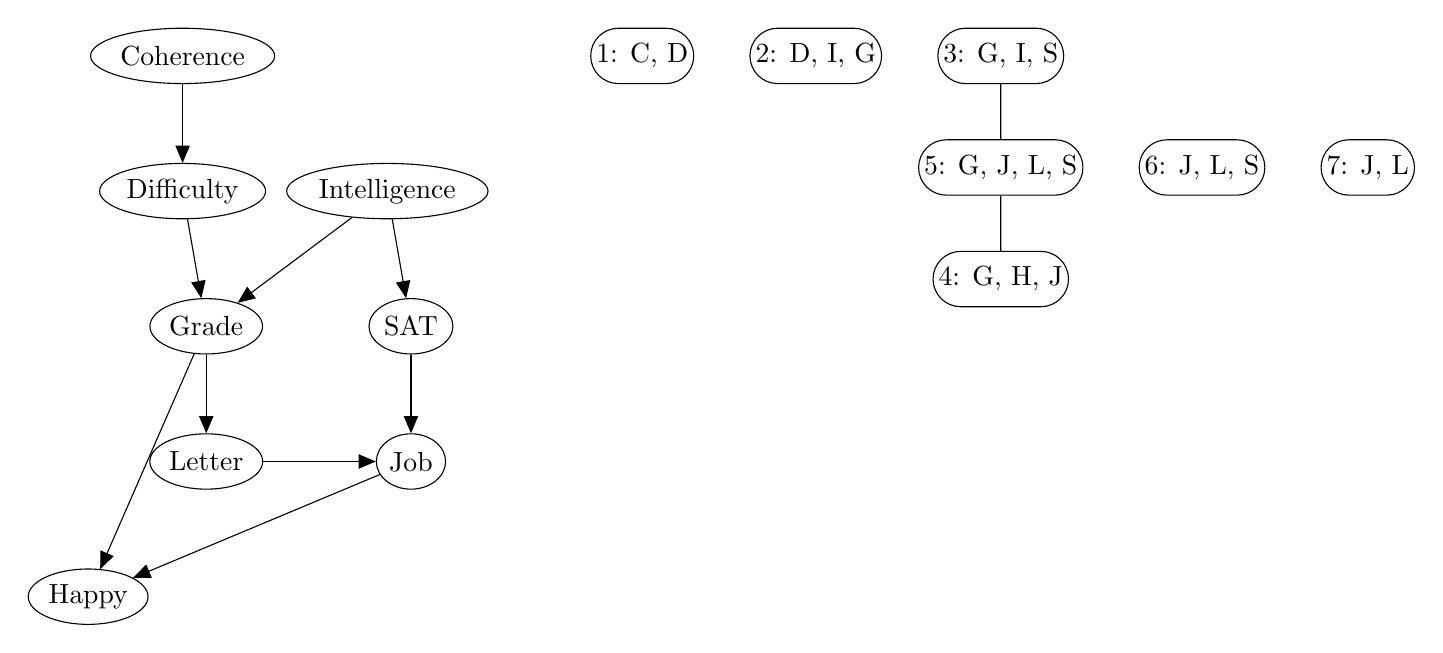
\begin{tikzpicture}[font=\sffamily]
	
	\node[latent, ellipse] (C) {Coherence};
	\node[latent, ellipse, below=of C] (D) {Difficulty};asf
	\node[latent, ellipse, below=of C, xshift=2.6cm] (I) {Intelligence};
	
	\node[latent, ellipse, below=of D, xshift=0.3cm] (G) {Grade}; 
	\node[latent, ellipse, below=of I, xshift=0.3cm] (S) {SAT};
	
	\node[latent, ellipse, below=of G] (L) {Letter};
	\node[latent, ellipse, below=1cm of S] (J) {Job};
	\node[latent, ellipse, below=of L, xshift=-1.5cm] (H) {Happy};
	
	\edge{C} {D};
	\edge{D} {G};
	\edge{I} {G, S};
	\edge{S} {J};
	\edge{G} {L, H};
	\edge{L} {J};
	\edge{J} {H};
	
	
	\node[latent, rounded rectangle, right=4cm of C] 	(CD) 	{1: C, D};
	\node[latent, rounded rectangle, right=0.7cm of CD]  		(DIG) 	{2: D, I, G};
	\node[latent, rounded rectangle, right=0.7cm of DIG]		(GIS) 	{3: G, I, S};
	\node[latent, rounded rectangle, below=0.7cm of GIS]		(GJLS) 	{5: G, J, L, S};
	\node[latent, rounded rectangle, below=0.7cm of GJLS]		(GHJ) 	{4: G, H, J};
	\node[latent, rounded rectangle, right=0.7cm of GJLS]		(JLS) 	{6: J, L, S};
	\node[latent, rounded rectangle, right=0.7cm of JLS]		(JL) 	{7: J, L};
	
	\medge[-] {CD} 		{DIG} {D};
	\medge[-] {DIG} 	{GIS} {G,I};
	\edge[-] {GIS, GHJ}	{GJLS};
	\medge[-] {GJLS} {JLS} {J,S,L};
	\medge[-] {JLS} {JL} {J,L};
	\end{tikzpicture}
\end{center}

\myspace
\p \blue{Clique Trees}. Since VE uses each intermediate $\tau_i$ at most once, the cluster graph induced by an execution VE is necessarily a \textit{tree}, and it also defines a directionality: the direction of the message passing (left-to-right in the above illustration). All the messages flow toward a single cluster where the final result is computed -- the \textbf{root} of the tree; we say the messages ``flow up'' to the root. Furthermore, for cluster trees induced by VE, the scope of each message (edge) $\tau_i$ is \textit{exactly} $\matr[i]{C} \cap \matr[j]{C}$, not just a subset\footnote{This follows from the \green{running intersection property}, which is satisfied by any cluster tree that's defined by variable elimination. It's defined as, if any variable $X$ is in both cluster $\matr[i]{C}$ and $\matr[j]{C}$, then $X$ is also in every cluster in the (unique) path in the tree between $\matr[i]{C}$ and $\matr[j]{C}$.}.
\vspace{-0.7em}
\begin{quote}
	{\itshape Let $\Phi$ be a set of factors over $\mathcal X$. A cluster tree over $\Phi$ that satisfies the running intersection property is called a \green{clique tree}. For clique trees, the clusters are also called \green{cliques}. }
\end{quote}


\myspace
\p \blue{Message Passing: Sum Product}. Previously we saw how an execution of VE can be illustrated with a clique tree. We now go the other direction -- given a clique tree, we show how it can be used for variable elimination. Given a clique tree representation of some BN, we can use it to guide us along an execution of VE to compute any marginal we'd like. First, before any run, we generate the set of \green{initial potentials} $\psi_i$ associated with each clique $\matr[i]{C}$ in the tree, defined as just the multiplication of the initial factors associated with the clique. We define the root of the tree as any clique containing the variable whose marginal we want to compute (we pick arbitrarily). Starting from the leaves and moving toward the root, we pass messages along from clique to clique. A clique is \textit{ready} to send a message when it has received a message from all of its downstream neighbors. The message from $\matr[i]{C}$ to [a neighbor] $\matr[j]{C}$ is computed using the \green{sum-product message passing} computation:
\graybox{
	\delta_{i \rightarrow j} &= \sum_{ \matr[i]{C} - \matr[i,j]{S}  }	\psi_i \cdot \prod_{k \in ( Nb_i - \{j\}   )} \delta_{k \rightarrow i} \tlab{10.2}
}
where the summation is simply over the variables in $\matr[i]{C}$ that aren't passed along to $\matr[j]{C}$, and the product is over all messages that $\matr[i]{C}$ received. Stated even simpler, we multiply all the incoming messages by our initial potential, then sum out all variables except those in $\matr[i,j]{S}$. When the root clique has received all messages, it multiplies them with its own initial potential, resulting in a factor called the \green{beliefs}, $\beta_r(\matr[r]{C})$. It represents
\begin{align}
	\widetilde{P}_{\Phi}(\matr[r]{C}) = \sum_{\mathcal X - \matr[r]{C}} \prod_{\phi} \phi
\end{align}
where, to be clear, the product is over all $\phi$ in the graph. \\

\p Below is a more compact summary of all of this, showing the procedure for computing \textit{all} final factors (belief) $\beta_i$ for some marginal probability query on the variables in $\matr[r]{C}$ \textit{asynchronously}. \\ 
\purple{Algorithm 10.2: Sum-Product Belief Propagation}
\begin{compactenum}
	\item For each clique $\matr[i]{C}$, compute its initial potential:
	$$
		\psi_i(\matr[i]{C}) \leftarrow \prod_{\phi_j : \alpha(\phi_j)=i }\big[  \phi_j  \big]
	$$
	
	\item While $\exists i,j$ such that $i$ is ready to transmit to $j$, compute:
	$$
		\delta_{i \rightarrow j} \leftarrow \sum_{ \matr[i]{C} - \matr[i,j]{S}  }	\psi_i \cdot \prod_{k \in ( Nb_i - \{j\}   )} \delta_{k \rightarrow i}
	$$
	
	\item Then, compute each belief factors $\beta_i$ by multiplying the initial potential $\psi_i$ by the incoming messages to $\matr[i]{C}$:
	$$
		\beta_i \leftarrow \psi_i \cdot \prod_{k \in Nb_{C_i}} \delta_{k \rightarrow i}
	$$
	
	\item Return the set of beliefs $\{ \beta_i \}$, where 
	\begin{align}
		\beta_i = \sum_{\mathcal{X} - \matr[i]{C}} \widetilde{P}_{\Phi}(\mathcal{X}) =  \widetilde{P}_{\Phi}(\matr[i]{C})
	\end{align}
\end{compactenum}
The SP Belief Propagation algorithm above is also called \green{clique tree calibration}. A clique tree $\mathcal{T}$ is \textit{calibrated} if all pairs of adjacent cliques are calibrated. A calibrated clique tree satisfies the following property for what we'll now call the \green{clique beliefs}, $\beta_i$, and the \green{sepset beliefs}, $\mu_{i,j}$ over $\matr[i,j]{S}$:\marginnote{$\mu_{i,j} = \widetilde{P}_{\Phi}(\matr[i,j]{S})$}[3em]
\graybox{
	\mu_{i,j}(\matr[i,j]{S}) \triangleq \sum_{\matr[i]{C} - \matr[i,j]{S}} \beta_i  &= \sum_{\matr[j]{C} - \matr[i,j]{S}} \beta_j 
}
\vspace{-0.5em}
\begin{quote}
	{\itshape\small
	The main advantage of the clique tree algorithm is that it computes the posterior probability of all variables in a graphical model using only twice the computation\footnote{The algorithm is equivalent to doing one upward pass, one downward pass.} of the upward pass in the same tree. 
	}
\end{quote}
We can also show that $\mu_{i,j} = \delta_{j \rightarrow i} \delta_{i \rightarrow j}$, which then allows us to derive:
\begin{align}
	\widetilde{P}_{\Phi}(\mathcal X) &= \dfrac{ \prod_{i \in \mathcal{V}_{\mathcal T}} \beta_i
		}{  \prod_{ij \in \mathcal{E}_{\mathcal T}} \mu_{i,j}  } 
	\tlab{10.10}
\end{align}
In other words, the clique and sepset beliefs provide a \green{reparameterization} of the unnormalized measure, a property called the \green{clique tree invariant}.

\myspace
\p \blue{Message Passing: Belief Update}. We know discuss an alternative message passing approach that is mathematically equivalent but intuitively different than the sum-product approach. First, we introduce some new definitions.

\p \textbf{Factor Division}:\marginnote{Define 0/0 = 0}[3em]
\vspace{-1em}
\begin{quote}
	{\itshape Let $\X$ and $\Y$ be disjoint sets of variables, and let $\phi_1(\X, \Y)$ and $\phi_2(\Y)$ be two factors. We define the division of $\phi_1$ and $\phi_2$ as a factor $\psi$ with scope $\X, \Y$ as follows:
		$$
		\psi(\X, \Y) \triangleq \frac{  \phi_1(\X, \Y)  }{  \phi_2(\matr Y)}
		$$
	}
\end{quote}
Looking back at equation \ref{10.2}, we can now see that another way to write $\delta_{i \rightarrow j}$ is
\begin{align}
	\delta_{i \rightarrow j} = \frac{ \sum_{\matr[i]{C} - \matr[i,j]{S}} \beta_i }{ \delta_{j \rightarrow i} } \tlab{10.13}
\end{align}
Now, consider the clique tree below for the simple Markov network A-B-C-D:
\vspace{-0.5em}
\begin{center}
	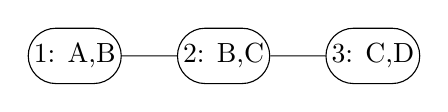
\begin{tikzpicture}[font=\sffamily]
	
	\node[latent, rounded rectangle] 							(AB) 	{1: A,B};
	\node[latent, rounded rectangle, right=0.7cm of AB]  		(BC) 	{2: B,C};
	\node[latent, rounded rectangle, right=0.7cm of BC]		(CD) 	{3: C,D};
	
	\edge[-] {AB} 		{BC};
	\edge[-] {BC} 		{CD};
	\end{tikzpicture}
\end{center}
\vspace{-0.5em}
If we assigned $\matr[2]{C}$ as the root, then our previous approach would compute $\delta_{2 \rightarrow 1}$ as $\sum_C \psi_2 \cdot \delta_{3 \rightarrow 2}$. Alternatively, we can use equation \ref{10.13} to realize this is equivalent to dividing $\beta_2$ by $\delta_{1 \rightarrow 2}$ and marginalizing out $C$. This observation motivates the algorithm below, which allows us to execute message passing in terms of the clique and sepset beliefs, without having to remember the initial potentials $\psi_i$ or explicitly compute the messages $\delta_{i \rightarrow j}$. 

\purple{Algorithm 10.3: Belief-Update Message Passing}
\begin{compactenum}
	\item For each clique $\matr[i]{C}$, set its initial belief $\beta_i$ to its initial potential $\psi_i$. For each edge in $\mathcal{E}_{\mathcal T}$, set $\mu_{i,j} = \mathbf{1}$.
	
	\item Wile there exists an uninformed\footnote{A clique is informed once it has received informed messages from all of its neighbors. An informed message is one that has been sent by taking into account information from all of the sending cliques' neighbors (aside from the receiving clique of that message, of course).} clique in $\mathcal T$, select any edge in $\mathcal{E}_{\mathcal T}$, and compute
	\graybox{
		\sigma_{i \rightarrow j} &\leftarrow \sum_{ \matr[i]{C} - \matr[i,j]{S} } \big[  \beta_i \big] \\
		\beta_j &\leftarrow \beta_j \cdot \frac{ \sigma_{i \rightarrow j} }{  \mu_{i,j}  } \\
		\mu_{i,j} &\leftarrow \sigma_{i \rightarrow j}
	}
	
	\item Return the resulting set of informed beliefs $\{ \beta_i \}$. 
\end{compactenum}
At convergence, $\sigma_{i \rightarrow j} = \mu_{i,j} = \sigma_{j \rightarrow i}$. 









% ======================================================================================
\lecture{Probabilistic Graphical Models}{Inference as Optimization (Ch. 11)}{June 02, 2018}
% ======================================================================================
\vspace{-1.7em}
{\scriptsize Koller and Friedman (2009). Inference as Optimization.\\ \textit{Probabilistic Graphical Models: Principles and Techniques}.\\ }

\p \blue{Propagation-Based Approximation}. We can use a general-purpose cluster graph rather than the more restrictive clique tree (needed to guarantee exact inference) for approximate inference methods. Consider the simple Markov network below on the left.


\begin{center}
	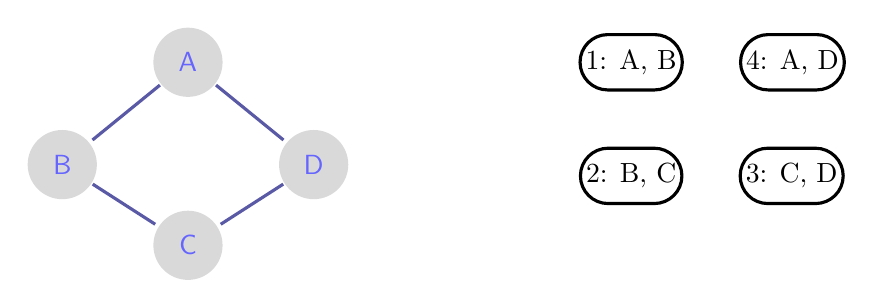
\begin{tikzpicture}[font=\sffamily,node distance=1.cm,->,>=latex,auto,line width=0.4mm]
	
	
	\tikzset{node st/.style={state, draw=none,
			fill=gray!30!white,
			text=blue!60!white}}
	\tikzset{node obs/.style={state, draw=none,
			fill=gray!60!black,
			text=blue!20!white}}
	
	\node[node st] (A) {A};
	\node[below=2em of A] (dummy) {};
	\node[node st, left=of dummy] (D) {B};
	\node[node st, right=of dummy] (B) {D};  
	\node[node st, below=4em of A] (C) {C};
	
	\draw[every loop,
	auto=right,
	draw=blue!30!gray]
	(A) edge[-] node{} (B)
	(A) edge[-] node{} (D)
	(B) edge[-] node{} (C)
	(D) edge[-] node{} (C);
	
	
	
	\node[latent, rounded rectangle, right=4.5cm of A] 	(AB) 	{1: A, B};
	\node[latent, rounded rectangle, right=0.7cm of AB] (AD) 	{4: A, D};
	\node[latent, rounded rectangle, below=0.7cm of AB] (BC) 	{2: B, C};
	\node[latent, rounded rectangle, right=0.7cm of BC] (CD) 	{3: C, D};

	
	\medge[-] {AB} 		{AD} {A};
	\medge[-] {AB}		{BC} {\hspace*{-0.2cm}B};
	\medge[-] {BC} 		{CD} {C};
	\medge[-] {AD} 		{CD} {\hspace*{0.2cm}D}
	\end{tikzpicture}
\end{center}

The clique tree for this network, which can be used for exact inference, has two cliques ABD and BCD and messages are passed between them consisting of $\tau(B, D)$. Suppose that, instead, we set up 4 clusters corresponding to each of the initial potentials, shown as the cluster graph above on the right. We can still apply belief propagation here, but due to it now having loops (as opposed to before when we only had trees), \textit{the process may not converge}. 













% ======================================================================================
\lecture{Probabilistic Graphical Models}{Parameter Estimation (Ch. 17)}{June 17, 2018}
% ======================================================================================
\vspace{-1.7em}
{\scriptsize Koller and Friedman (2009). Parameter Estimation.\\ \textit{Probabilistic Graphical Models: Principles and Techniques}.\\ }

\p \blue{Maximum Likelihood Estimation} (17.1). In this chapter, assume the network structure is fixed and that our data set $\mathcal D$ consists of fully observed instances of the network variables: $\mathcal D = \{ \xi[1], \ldots, \xi[M] \}$. We begin with the simplest learning problem: parameter learning for a single variable. We want to estimate the probability, denoted via the \textit{parameter} $\theta$, with which the flip of a thumbtack will land heads or tails. Define the \green{likelihood function} $L(\theta : \vec{x})$ as the probability of observing some sequence of outcomes $\vec{x}$ under the parameter $\theta$. In other words, it is simply $P(\vec x : \theta)$, but interpreted as a \textit{function of $\theta$}. For our simple case, where $\mathcal D$ consists of $M$ thumbtack flip outcomes,
\begin{align}
	L(\theta : \mathcal D) &= \theta^{M[1]} (1 - \theta)^{M[0]}
\end{align}
where $M[1]$ denotes the number of outcomes in $\mathcal D$ that were heads. Since it's easier to maximize a logarithm, and since it yields the same optimal $\hat \theta$, optimize the \green{log-likelihood} to obtain:
\begin{align}
	\hat \theta &= \argmax_{\theta} \ell (\theta : \mathcal D) = \argmax_{\theta} \big[ M[1] \log\theta + M[0]\log(1 - \theta) \big] \\
	&= \frac{ M[1] }{ M[1] + M[0] }
\end{align}
Note that MLE has the \textit{disadvantage} that it can't communicate confidence of an estimate\footnote{We get the same result (0.3) if we get 3 heads out of 10 flips, as we do for getting 300 heads out of 1000 flips; yet, the latter experiment should include a higher degree of confidence}. \\

We now provide the more general formal definitions for MLE. 
\begin{compactitem}
	\item We are given a \textit{training set} $\mathcal D$ containing $M$ (IID) instances of a set of random variables $\mathcal X$, where the samples of $\mathcal X$ are drawn from some unknown distribution $P^*(\mathcal X)$. 
	
	\item We are given a \green{parametric model}, defined by a function $P(\xi ; \vec{\theta})$, where $\xi$ is an instance of $\mathcal X$, and we want to estimate its parameters $\vec{\theta}$\footnote{We also have the constraint that $P(\xi ; \vec{\theta})$ must be a valid distribution (nonnegative and sums to 1 over all possible $\xi$)}. The model also defines the space of legal parameter values $\Theta$, the \green{parameter space}. 
	
	\item We then define the \green{likelihood function} $L(\vec{\theta} : \mathcal D) = \prod_m P(\xi[m] : \vec{\theta})$. 
\end{compactitem}

\p We can often simplify the likelihood function to simpler terms, like our $M[0]$ and $M[1]$ values in the thumbtack example. These are called the \green{sufficient statistics}, defined as functions of the data that summarize the relevant information for computing the likelihood. Formally,
\vspace{-0.5em}
\begin{quote}
	{\small\itshape 
		A function $\tau(\xi) : \xi \rightarrow \R^{\ell}$ (for some $\ell$) is a \green{sufficient statistic} if for any two data sets $\mathcal D$ and $\mathcal{D}'$, we have that
		\graybox{
			\bigg[ \sum_{ \xi[m] \in \mathcal D } \tau(\xi[m])	 = \sum_{ \xi'[m] \in \mathcal D' } \tau(\xi'[m]) \bigg]
			\implies 
			\bigg[ L(\vec{\theta} : \mathcal D) = L(\vec{\theta} : \mathcal D')    \bigg]
		} 
		\textbf{We often informally refer to the tuple $\sum_{\xi[m] \in mathcal D} \tau(\xi[m])$ as the sufficient statistics of the data set $\mathcal D$.}
	}
\end{quote}

\myspace
\p \blue{MLE for Bayesian Networks -- Simple Example}. We now move on to estimating parameters $\vec{\theta}$ for the simple BN $X \rightarrow Y$ for two binary RVs $X$ and $Y$. Our parameters $\vec{\theta}$ are the individual probabilities of $P(X)$ and $P(Y \mid X)$ (6 total). Since BNs have the nice property that their joint probability decomposes into a product of probabilities, just like how the likelihood function is a product of probabilities, we can write the likelihood function as a product of the individual \textit{local} probabilities:\marginnote{decomposability of the likelihood function}[2em]
\begin{align}
	L(\vec{\theta} : \mathcal D) &= \bigg( \prod_m P(x[m] : \vec[X]{\theta})  \bigg) \bigg( \prod_m P(y[m] \mid x[m] : \vec[Y \mid X]{\theta}) \bigg)
\end{align}
which can be decomposed even further by e.g. differentiating products over $x[m]:x[m]=x^0$ etc. Just as we used $M[0]$ in the thumbtack example to count the number of instances with a certain value, we can use the same idea for the general case. 
\vspace{-0.5em}% TODO: 19.{1.1, 1.3, 2.2}
\begin{quote}
	{\small\itshape
		Let $\Z$ be some set of RVs, and $\vec{z}$ be some instantiation to them. We define $M[\vec{z}]$ to be the number of entries in data set $\mathcal D$ that have $\Z[m] = \vec{z}$:
		\begin{align}
			M[\vec z] &= \sum_m \ind\{\Z[m] = \vec z \}
		\end{align}
	}
\end{quote}


\myspace
\p \blue{Global Likelihood Decomposition}. We now move to the more general case of computing the likelihood for BN with structure $\mathcal G$.\marginnote{global decomposition of the likelihood}[2em]
\begin{align}
	L(\vec{\theta} : \mathcal D) &= \prod_m P_{\mathcal G} (\xi[m] : \vec{\theta}) \\
	&= \prod_m \prod_i P(x_i[m] \mid Pa_{X_i}[m] : \vec{\theta}) \\
	&= \prod_i \bigg[ \prod_m  P(x_i[m] \mid Pa_{X_i}[m] : \vec[X_i \mid Pa_{X_i}]{\theta})  \bigg] \\
	&= \prod_i L_i (\vec[X_i \mid Pa_{X_i}]{\theta} : \mathcal D)
\end{align}
where $L_i$ is the \green{local likelihood function} for $X_i$. Assuming these are each disjoint sets of parameters from one another, it implies that $\hat{\vec{\theta}} = \langle \vec[X_1 \mid Pa_{X_1}]{\hat{\theta}}, \ldots, \vec[X_n \mid Pa_{X_n}]{\hat{\theta}}   \rangle$







% ======================================================================================
\lecture{Probabilistic Graphical Models}{Partially Observed Data (Ch. 19)}{June 17, 2018}
% ======================================================================================
\vspace{-1.7em}
{\scriptsize Koller and Friedman (2009). Partially Observed Data.\\ \textit{Probabilistic Graphical Models: Principles and Techniques}.\\ }

\p \blue{Likelihood of Data and Observation Models} (19.1.1). Consider the simple example of flipping a thumbtack, but occasionally the thumbtack rolls off the table. We choose to ignore the tosses for which the thumbtack rolls off. Now, in addition to the random variable $X$ giving the flip outcome, we have the \textit{observation variable} $O_X$, which tells us whether we observed the value of X. 
\begin{center}
	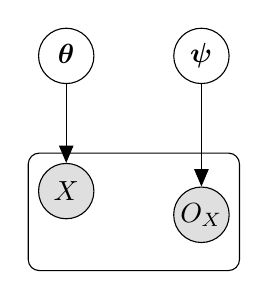
\begin{tikzpicture}[font=\sffamily]
	\node[latent] (theta) {$\vec{\theta}$};
	\node[obs, below=of theta] (X) {$X$};
	\edge{theta} {X};
	
	\node[latent, right=of theta] (psi) {$\vec\psi$};
	\node[obs, below=1.3cm of psi] (OX) {$O_X$};
	\edge{psi} {OX};
	
	\plate {p} {(X)(OX)} {} ;
	\end{tikzpicture}
\end{center}
The illustration above is a plate model where we choose a thumbtack sampled with bias $\vec{\theta}$ and repeat some number of flips with that same thumbtack. We also sample the random variable $O_X$ that has probability of observation sampled from $\psi$ and fixed for all the experiments we do. This leads to the following definition for the observability model. 
\vspace{-0.5em}
\begin{quote}
	{\small\itshape
		Let $\X = \{X_1, \ldots X_n \}$ be some set of RVs, and let $O_{\X} = \{ O_{X_1}, \ldots, O_{X_n}  \}$ be their \green{observability variable}. The \green{observability model} is a join distribution $$P_{missing}(\X, O_{\X}) = P(\X) \cdot P_{missing}(O_{\X} \mid \X)$$so that $P(\X)$ is parameterized by $\vec{\theta}$ and $P_{missing}(O_{\X} \mid \X)$ is parameterized by $\vec{\psi}$. We define a new set of RVs $\Y = \{Y_1, \ldots Y_n \}$ where $Val(Y_i) = Val(X_i) \cup \{?\}$. The actual observation $\Y$ is a deterministic function of $\X$ and $O_{\X}$:
		\begin{align}
			Y_i = \begin{cases}
				X_i & O_{X_i} = o^1 \\
				? & O_{X_i} = o^0
			\end{cases}
		\end{align}
	}
\end{quote}
For our simple model above, we have
\begin{align}
	P(Y = 1) &= \theta \psi \\
	P(Y = 0) &= (1 - \theta) \psi \\
	P(Y = ?) &= (1 - \psi) \\
	L(\theta, \psi; \mathcal D) &= \theta^{M[1]}(1 - \theta)^{M[0]}\psi^{M[1] + M[0]} (1 - \psi)^{M[?]}
\end{align}
The main takeaway is to understand that \textbf{when we have missing data, the data-generation process involves two steps: (1) generate data by sampling from the model, then (2) determine which values we get to observe and which ones are hidden from us}. 


\myspace \p \blue{The Likelihood Function} (19.1.3). Assume we have a BN network $\mathcal G$ over a set of variables $\X$. In general, each instance has a different set of observed variables. Denote by $\matr{O}[m]$ and $\vec{o}[m]$ the observed vars and their values in the $m$'th instance, and by $\matr{H}[m]$ the missing (or hidden) vars in the $m$'th instance. 

% \myspace \p \blue{Expectation Maximization (EM)} (19.2.2). 























\begin{comment}

INFERENCE TRACK:
% ======================================================================================
\lecture{Probabilistic Graphical Models}{Clique Trees (Ch. 10)}{May 06, 2018}
% ======================================================================================
% TODO: 10.1 - 10.2
% ======================================================================================
\lecture{Probabilistic Graphical Models}{Inference as Optimization (Ch. 11)}{May 06, 2018}
% ======================================================================================
% TODO: 11.{3.1-3.5}
% ======================================================================================
\lecture{Probabilistic Graphical Models}{Particle-Based Approximate Inference (Ch. 12)}{May 06, 2018}
% ======================================================================================
% TODO: 12.{1, 3.1-3.3}



\begin{center}
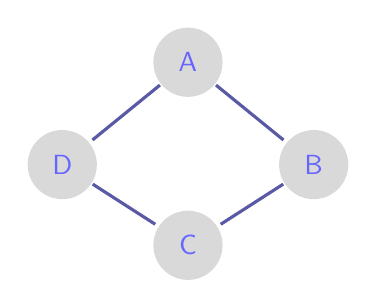
\begin{tikzpicture}[font=\sffamily,node distance=1.cm,->,>=latex,auto,line width=0.4mm]


\tikzset{node st/.style={state, draw=none,
fill=gray!30!white,
text=blue!60!white}}
\tikzset{node obs/.style={state, draw=none,
fill=gray!60!black,
text=blue!20!white}}

\node[node st] (A) {A};
\node[below=2em of A] (dummy) {};
\node[node st, left=of dummy] (D) {D};
\node[node st, right=of dummy] (B) {B};  
\node[node st, below=4em of A] (C) {C};

\draw[every loop,
auto=right,
draw=blue!30!gray]
(A) edge[-] node{} (B)
(A) edge[-] node{} (D)
(B) edge[-] node{} (C)
(D) edge[-] node{} (C);
\end{tikzpicture}
\end{center}

LEARNING TRACK
% ======================================================================================
\lecture{Probabilistic Graphical Models}{Learning Graphical Models: Overview (Ch. 16)}{May 06, 2018}
% ======================================================================================
% TODO: ALL
% ======================================================================================
\lecture{Probabilistic Graphical Models}{Parameter Estimation (Ch. 17)}{May 06, 2018}
% ======================================================================================
% TODO: 17.{1,2}
% ======================================================================================
\lecture{Probabilistic Graphical Models}{Partially Observed Data (Ch. 19)}{May 06, 2018}
% ======================================================================================
% TODO: 19.{1.1, 1.3, 2.2}

\end{comment}



\renewcommand{\Z}{\mathbb{Z}}
% ==================================================================================
% ==================================================================================
% ==================================================================================
% ITILA
% ==================================================================================
% ==================================================================================
% ==================================================================================
\mysection{Information Theory, Inference, and Learning Algorithms}\label{Information Theory, Inference, and Learning Algorithms}


% ======================================================================================
\lecture{Information Theory, Inference, and Learning Algorithms}{Introduction to Information Theory (Ch. 1)}{November 11, 2017}
% ======================================================================================

{\footnotesize [Note: Skipping most of this chapter since it's mostly introductory material.]}

\p \blue{Preface}. For ease of reference, some common quantities we will frequently be using: 
\begin{compactitem}
	\item \textbf{Binomial distribution}. Let $r$ denote the number of successful trials out of $N$ total trials. Let $f$ denote the probability of success for a single trial.
	\begin{align}
	\Prob{r \mid f, N} = \binom{N}{r} f^r (1 - f)^{N - r} \qquad
	\E{r} = Nf \qquad
	\Var{r} = Nf(1-f)
	\end{align}
	
	\item \textbf{Stirling's Approximation}.\marginnote{Recall that $\log_b x = \frac{\log_a x}{\log_a b}$}[2em]
	\begin{align}
	x! \simeq x^x e^{-x} \sqrt{2 \pi x} 
	\quad &\Leftrightarrow \quad
	\ln x! \simeq x \ln x - x + \onehalf \ln 2 \pi x \\
	\ln\binom{N}{r} &\simeq r \ln \frac{N}{r} + (N - r) \ln \frac{N}{N - r}
	\end{align}
	
	\item \textbf{Binary Entropy Function} and its relation with Stirling's approximation.
	\begin{align}
	H_2(x) &\triangleq x \lg \inv{x} + (1-x) \lg \inv{1 - x} \\
	\lg \binom{N}{r} &\simeq N H_2(r/N)
	\end{align}
\end{compactitem}

\myspace
\p \blue{Perfect communication over an imperfect, noisy communication channel (1.1)}. We want to make an encoder-decoder architecture, of the general form in the figure below, to achieve reliable communication over a noisy channel.
\myfig[0.55\textwidth]{ITILA_1_6.png} 

\green{Information theory} is concerned with the theoretical limitations and potentials of such systems. Let's explore some examples for the case of the \green{binary symmetric channel}\footnote{A binary symmetric channel transmits each bit correctly with probability (1 - f) and incorrectly with probability f, where $f$ is assumed to be small.}:
\begin{compactitem}
	\item \textbf{Repetition codes}. Let $R_N$ denote the repetition code that repeats each bit in the message $N$ times\footnote{So $R_2$ would encode $101$ as $110011$.}. We model the channel as ``adding\footnote{We add in modulo 2, which is NOT the same as binary arithmetic (no carry). Addition modulo 2 is the same as doing XOR.}'' a sparse noise vector $\vec{n}$ to the encoded message $\vec{t}$, so $\vec{r} := \vec{n} + \vec{t}$. What is the optimal way of decoding $r$?
	\begin{align}
	\hat{s_i} &\leftarrow \argmax_{s_i} \Prob{ s_i \mid \vec[i:i+n]{r} } = \argmax_{s_i} \Prob{ \vec[i:i+N]{r} \mid s_i } \Prob{ s_i } 
	\end{align}
	We see that we must make assumptions about the prior probability $\Prob{s_i}$. It is common to assume all possible values of $s_i$ (0 or 1 in this case) are equally probable. It is useful to observe the \green{likelihood ratio},
	\begin{align}
	\frac{  \Prob{ \vec[i:i+N]{r} \mid s_i = 1 }  }{   \Prob{ \vec[i:i+N]{r} \mid s_i = 0 } }
	&= \prod_{n = i}^{i + N - 1} \frac{  \Prob{ r_n \mid t_n = 1 }  }{   \Prob{ r_n \mid t_n = 0 } } 
	=  \prod_{n = i}^{i + N - 1} \begin{cases}
	\gamma & \text{if } r_n = 1 \\
	\gamma^{-1} & \text{if } r_n = 0
	\end{cases}
	\end{align}
	where we've defined $\gamma := (1 - f) / f$, with $f$ being the probability of a bit getting flipped by the channel. We want to assign $\hat s_i$ to the most likely \green{hypothesis} out of the possible $s_i$. If the likelihood ratio [for the two hypotheses] is greater than 1, we choose $\hat s_i = 1$, else we choose $ \hat s_i = 0$.  
	
	\item \textbf{Block Codes - the (7, 4) Hamming Code}. Although, by increasing the number of repetitions per bit $N$ for our $R_N$ repetition code can decrease the error-per-bit probability $p_b$, we incur a substantial decrease in the \textit{rate of information transfer} -- a factor of 1/N. The \green{(7, 4) Hamming Code} tries to improve this by encoding \textit{blocks} of bits at a time (instead of per-bit). It is a \textit{linear block code} -- it encodes each 4-bit block into a 7-bit block, where the additional 3 bits are linear functions of the original $K=4$ bits. The $(7, 4)$ Hamming code has each of the extra 3 bits act as parity checks. It's easiest to show this with the illustration below:
	\myfig[0.4\textwidth]{ITILA_1_13.png}
	
	which encodes \texttt{1000} as \texttt{1000101}.
\end{compactitem}



% ======================================================================================
\lecture{Information Theory, Inference, and Learning Algorithms}{Probability, Entropy, and Inference (Ch. 2)}{November 12, 2017}
% ======================================================================================

{\footnotesize [Note: Skipping most of this chapter since it's mostly introductory material.]}

\myspace
\p \blue{Notation}. Some of the notation this author seems to use a lot.
\begin{compactitem}
	\item \textbf{Ensemble} $X$: a triple $(x, \mathcal{A}_X, \mathcal{P}_X)$, where the outcome $x$ is the value of a R.V. which can take on one of a set of possible values (``alphabet''), $\mathcal{A}_X = \{a_1, \ldots, a_i, \ldots, a_I\}$, having probabilities $\mathcal{P}_X = \{p_1, \ldots, p_i, \ldots p_I\}$. Note that this doesn't appear technically consistent with how the author actually \textit{uses} the term ensemble -- in practice, he actually means ``$X$ is the \underline{set of all possible} triples $(x, \mathcal{A}_X, \mathcal{P}_X), \forall x \in \mathcal{A}_X$, or something like that. He uses it to casually refer to the space of possibilities.
\end{compactitem}

\myspace
\p \blue{Forward Probabilities and Inverse Probabilities}. Both of these involve a \green{generative model} of the data. In a \textit{forward} probability problem, we want find the PDF, expectation, or some other function of a quantity that depends on the data/is \textit{produced} by the generative process. For example, we can model a series of $N$ coin flips as ``producing'' the quantity $n_H$, denoting the number of heads. In an \textit{inverse} probability problem, we want to compute conditional probabilities on one or more of the \textit{unobserved variables} in the process, \textit{given} the observed variables. 

\myspace
\p \blue{The Likelihood Principle}. For a generative model on data $d$ given parameters $\vec\theta$, $\Prob{d \mid \vec\theta}$, and having observed a particular outcome $d_1$, all inferences and predictions should depend only on the function $\Prob{d_1 \mid \vec\theta}$. 

\myspace
\p \blue{Entropy and Related Quantities}.
\begin{compactitem}[-]
	\item \textbf{Shannon information content} of an outcome $x$:
	\begin{align}
		h(x) \triangleq \lg \left( \inv{P(x)} \right)
	\end{align}
	
	\item \textbf{Entropy of Ensemble $X$}. Defined to be the average Shannon information content of an outcome.\marginnote{$$ 0 \times \lg \left( \inv{0} \right) \triangleq 0$$}
	\begin{align}
		H(X) &\triangleq \sum_{x \in \mathcal{A}_X} \Prob{x}  \lg \left( \inv{\Prob{x}} \right) \\
		H(X) &\le \lg \left( |\mathcal{A}_X| \right) \quad \text{with equality iff} \quad  p_i = \inv{\mathcal{A}_X} ~  \forall i
	\end{align}
	
	\item \textbf{Decomposability of the Entropy}. For any probability distribution $\vec p = \{p_1, p_2, \ldots, p_I\}$ and $m$ (where $1 \le m \le I$):
	\begin{align}
		H(\vec{p}) &= H\left( \Sigma_{1:m}, \Sigma_{m+1:I} \right) \\
		&+ \Sigma_{1:m} H\left( \frac{p_1}{\Sigma_{1:m}}, \ldots, \frac{p_m}{\Sigma_{1:m}} \right) \\
		&+ \Sigma_{m+1:I} H\left( \frac{p_{m+1}}{\Sigma_{m+1:I}}, \ldots, \frac{p_I}{\Sigma_{m+1:I}} \right)
	\end{align}
	where I've let $\Sigma_{1:m} := \imsum p_i$.
	
	\item \textbf{Kullback-Leibler Divergence} between two probability distributions $P(X)$ and $Q(X)$ that are defined over the same alphabet $\mathcal{A}_X$:
	\begin{align}
		D_{KL}(P||Q) &= \sum_x P(x) \lg \frac{P(x)}{Q(x)} \\
		 D_{KL}(P||Q) &\ge 0 \qquad \mtred{[Gibb's Inequality]} 
	\end{align}
	where, in the words of the author, ``\purple{Gibb's inequality is probably the most important inequality in this book}''.
	
	\item \textbf{Convex functions and Jensen's Inequality}. A function $f(x)$ is convex over the interval $[x=a, x=b]$ if every chord of the function lies above the function. That is, $\forall x_1, x_2 \in [a, b]$ and $0 \le \lambda \le 1$:
	\begin{align}
		f\left(  \lambda x_1 + (1 - \lambda) x_2 \right) &\le \lambda f(x_1) + (1 - \lambda) f(x_2) \\
		f\left( \E{x} \right) &\le \E{f(x)} \qquad \mtred{[Jensen's Inequality]} 
	\end{align}
	and we say $f$ is \green{strictly convex} if, $\forall x_1, x_2 \in [a, b]$, we get equality for only $\lambda=0$ and $\lambda=1$. 
\end{compactitem}

\myspace
\subsub{More About Inference (Ch. 3 Summary)}
\myspace

{\footnotesize Because this is too short to have as its own chapter...}


\p \blue{A first inference problem}. Author explores a particle decay problem of finding $\Prob{\lambda \mid \{x\}}$ where $\lambda$ is the characteristic decay length and $\{x\}$ is our collection of observed decay distances. Plotting the likelihood $\Prob{\{x\} \mid \lambda}$ \textit{as a function of $\lambda$} for any given $x \in \{x\}$ shows each has a \textit{peak} value. The kicker is the interpretation: if each measurement $x \in \{x\}$ is independent, the total likelihood is the product of all the individual likelihoods, which can be interpreted as updating/narrowing the interval $[\lambda_a, \lambda_b]$ within which $\Prob{\{x\} \mid \lambda}$ (as a function of $\lambda$) peaks. In the words of the author's mentor:
\begin{quote}
	{\itshape what you know about $\lambda$ after the data arrive is what you knew before ($\Prob{\lambda}$) and what the data told you ($\Prob{\{x\} \mid \lambda}$)}
\end{quote}
We update our beliefs regarding the distribution of $\lambda$ as we collect data.


\myspace
\p \blue{Lessons learned from problems}. 
\begin{compactitem}
	\item[(3.8)] The classic Monty Hall problem. \textbf{Be careful defining probabilities after collecting data}. My blunder: when using Bayes'theorem to get the probability of the prize being behind door $i \in \{1,2\}$ after the host opens door 3, I failed to take into account that we chose door 1 while I was computing the evidence (the marginal probability that the host opened door 3)\footnote{Note that, while important to recognize and understand, I could've avoided this pitfall entirely by just ignoring the evidence during calculations and normalizing after, since the evidence can be determined solely by the normalization constraint.}. Quite embarrassing. 
	
	\item[(3.9)] Monty Hall problem, but an earthquake opens door 3. Although I correctly answered that, in this case, both hypotheses (the prize being behind door 1 or door 2) are equiprobable, I still failed to account for the subtle fact that the earthquake could've opened \textit{multiple} doors. The lesson here is \textbf{always write down the probability of everything}, which just so happens to be suggested by the solution for this problem, too.\\
	
	So, why did I still get the answer correct? The reason is because enumeration of probabilities wasn't necessary at all, you just needed to realize that the likelihood for the two remaining hypotheses ($\mathcal{H}_1$ and $\mathcal{H}_2$) were the \textit{same} -- the probability of observing the earthquake open door 3 and the prize not being revealed was the same for the case of the prize being behind door 1 or door 2. So maybe the real lesson here is \textbf{determine whether calculations are even needed in order to solve the given problem}, which luckily I've had drilled in my head for years from studying physics. 
	
	\item[(3.15)] Another biased coin variant. One of the best examples I've seen for favoring Bayesian methods over frequentist methods. Also, made use of the beta function:
	\graybox{
		\int_{0}^{1} p^{x} (1 - p)^{y} \mathrm{d}p &= \frac{\Gamma (x + 1) \Gamma (y + 1)}{\Gamma (x + y + 2)} = B(x + 1, y + 1)
	}
	where $B$ is the \green{beta function}, which is defined by the LHS.
\end{compactitem}

% ======================================================================================
\lecture{Information Theory, Inference, and Learning Algorithms}{The Source Coding Theorem (Ch. 4)}{November 23, 2017}
% ======================================================================================

\p \blue{Overview}. We will be examining the two following assertions:
\begin{compactenum}
	\item The Shannon information content is a sensible measure of the information content of a given outcome $x = a_i$:
	\begin{align}
		h(x = a_i) \triangleq \lg\inv{p_i} \label{shannon-info-content}
	\end{align}
	
	\item The entropy of an ensemble $X$ is a sensible measure of the ensemble's average information content. 
	\begin{align}
		H(X) = \sum_i p_i \lg\inv{p_i}
	\end{align}
\end{compactenum}

\myspace
\p \blue{The weighing problem}. We are instructed to ponder the following problem. 
\vspace{-1em}
\begin{quote}
	{\itshape\footnotesize You're given 12 balls, all equal in weight except for one that is either heavier or lighter. You're also given a two-pan balance. Your task is to determine which ball is the odd ball, and in as few uses of the balance as possible. Note: each use of the balance must place the same number of balls on either side.}
\end{quote}
An interesting observation is to consider the number of possible outcomes of the weighing process. Each outcome can be one of three possibilities: equal weight, left heavier, or left lighter. After $N$ such weighings, the number of unique possible weighing result sequences is $3^N$. Note that there are $12 \times 2 = 24$ unique final answers for our task (identifying which is the odd ball, and whether it is heavier or lighter). Therefore, since we are seeking a procedure to identify which of the 24 options is the correct option with 100\% accuracy, we require our weighing procedure to take on \textit{at least} $24$ unique possible results. Since $N=3$ weighings corresponds to $3^N = 27$ possible outcomes, $N=3$ is a \textit{lower bound} on the number of weighings our approach will involve. It is \underline{impossible} to guarantee a correct answer for $N < 3$ weighings\footnote{Finally, it should be clear that, regardless of our approach, the final weighing will involve 2 balls, since we have to identify which is the oddball AND whether it is heavier/lighter AND the number of balls on the left of the scale must be the same as the right of the scale for every weighing.}. \\

Things I didn't consider until reading the solution:
\begin{compactitem}
	\item It's actually \textit{not} optimal, upon observing both sides equal, to subsequently use only the balls not involved in that measurement. My initial reaction to this was ``why? we already know the oddball is not any of the balls just measured, since the outcome was equal.'' The response to this reaction is: ``yes, \textit{exactly}, and we must use that information to be able to discern in the future whether, e.g., a measurement of ``left side heavier'' means the oddball is on the left and heavy, or if it's on the right and light -- \textit{it's useful to know that a given side of the scale does not contain the oddball before a measurement}.
	
	\item More generally, it's also not optimal to greedily search for solutions that eliminate the highest number of possibilities \textit{in any given single step}. Another way of thinking about this is that it's undesirable for the $i$th measurement outcome to cause any of the 3 possible measurement outcomes to be impossible at the next stage.
	
	\item I focused a disproportionate amount of thought on handling the equal-weight measurement outcome, for whatever reason. I probably would've arrived at the solution faster if I'd actually thought about how my strategies would've handled some outcome being ``left heavier'' and \textit{then considered what that strategy would put on the scale at the next step}, where the italics denote what would've illuminated the fatal flaw in all my approaches. 
\end{compactitem}


\myspace
\p \blue{Guessing Games}. What's the smallest number of yes/no questions needed to identify an integer $x$ between 0 and 63? Although it was obvious to me that the solution is to successively halve the possible values of $x$, I found it interesting that \textbf{you can write down the list of questions independent of the answers at each step} using a basic application of modular arithmetic. In other words, you can specify the full decision tree of $N$ nodes with just $\lg N$ questions. Nice. Also, recognize that the Shannon information content for any single outcome is $\lg\inv{0.5} = 1$ bit, and thus the total Shannon information content (for our predefined 6 questions) is 6 bits, which is not-coincidentally the number of possible values that $x$ could be before we ask any questions.\\

\p In general, if an outcome $x$ has Shannon information content $h(x)$ number of bits, I like to interpret that as ``learning the result $x$ eliminates $2^{h(x)}$ possibilities for the final result.'' The battleship example follows this interpretation well. Stated another way (in the author's words):
\begin{quote}
	{\itshape The Shannon information content can be intimately connected to the size of a file that encodes the outcomes of a random experiment.}
\end{quote}

\myspace
\subsub{Data Compression and Typicality}
\myspace

\p \blue{Data Compression}. A \green{lossy compressor} compresses some files, but maps some files to the \textit{same} encoding. We introduce a parameter $\delta$ that describes the risk (aggressiveness of our compression) we are taking with a given compression method: $\delta$ is the probability that there will be no name for an outcome\footnote{More specifically, if there is some subset, $\{a\}$, of unique values that $x$ can take on but our compression method discards/ignores, then we say $\delta = \sum_i p(x = a_i)$.} $x$.

\redbox[The smallest $\delta$-sufficient subset]{If $S_{\delta}$ is the smallest subset of $\mathcal{A}_X$ satisfying
\begin{align}
	\Prob{x \in S_{\delta}} \ge 1 - \delta
\end{align}
then $S_{\delta}$ is the smallest $\delta$-sufficient subset. It can be constructed by ranking the elements of $\mathcal{A}_X$ in order of decreasing probability and adding successive elements starting from the most probable elements until the total probability is $\ge (1 - \delta)$. 
}

\begin{compactitem}
	\item \green{Raw bit content} of $X$: $H_0(X) \triangleq \lg |\mathcal{A}_X|$. A lower bound for the number of binary questions that are always \textit{guaranteed} to identify an outcome from the ensemble X -- it simply maps each outcome to a constant-length binary string.
	
	
	\item \green{Essential bit content} of $X$: $H_{\delta}(X) \triangleq \lg |S_{\delta} |$. A compression code can be made by assigning a binary string of $H_{\delta}$ bits to each element of the smallest sufficient subset. 
\end{compactitem}

Finally, we can now state \green{Shannon's source coding theorem}: Let $X$ be an ensemble for the random variable $x$ with entropy $H(X) = H$ bits, and let $X^N$ denote a sequence of identically distributed (but not necessarily independent\footnote{Actually, before the actual theorem statement, the author mentions we are now concerned with ``string of $N$ i.i.d. random variables from a single ensemble $X$.'' It's probably fair to assume this is true for the quantities in the theorem, but I'm leaving this note here as a reminder.}) of random variables/ensembles, $(X_1, X_2, \ldots, X_N)$. 
\graybox{
	(\exists N_0 \in \Z^+)(\forall N > N_0 ): \qquad \left| 
		\inv{N} H_{\delta}(X^N) - H
	\right|	< \epsilon 
	\qquad (0 < \delta < 1) ~ (\epsilon > 0) \label{ssct}
}
which, in English, can be read: \textit{$N$ i.i.d. random variables each with entropy $H(X)$ can be compressed into more than $NH(X)$ bits with negligible risk of information loss, as $N \rightarrow \infty$; conversely if they're compressed into fewer than $NH(X)$ bits it is virtually certain that information will be lost.}

\myspace
\p \blue{Typicality}. The reason that large $N$ in equation \ref{ssct} corresponds to larger potential for better compression is that the subset of likely results for a string of outcomes becomes more and more concentrated relative to the number of possible sequences as $N$ increases\footnote{The author gave an example for a sequence of bits with probability of any given bit being 1 as 0.1. He showed how, although the \textit{average} number of 1s in a sequence of $N$ bits grew as $\mathcal{O}(N)$, the standard deviation of that average only grew as $\mathcal{\sqrt{N}}$.}. I just realized this is for the same fundamental reasons that entropy exists in thermodynamics -- \textit{there are just more ways to exist in a high entropy state than otherwise}. The author showed $\binom{N}{r}$ as a function of $r$ (the number of 1s in the N-bit string). For large $N$, this becomes almost comically concentrated near the center (like a delta function at $N/2$) -- see footnote for more details\footnote{The probability of getting a string with $r$ 1s follows a binomial distribution with mean $Np_1$ and standard deviation $\sqrt{Np_1(1-p_1)}$. This results in an increasingly narrower distribution $P(r)$ for larger $N$.}. \\

\p This motivates the notion of \green{typicality} for [a string of length $N$ from] an arbitrary ensemble $X$ with alphabet $\mathcal{A}_X$. For large $N$, we expect to find $p_i N$ occurrences of the outcome $x = a_i$. Hence the probability of such a string, and its information content, is roughly\footnote{We appear to be assuming that each outcome $x$ in the string $\vec x$ are i.i.d. (\textsc{confirmed})}
\begin{align}
	\Prob{\vec{x}}_{typ} &= \Prob{x_1} \Prob{x_2} \cdots \Prob{x_N} \simeq p_1^{(p_1N)} p_2^{(p_2 N)} \cdots p_I^{(p_I N)} \\
	h(\vec x)_{typ} &= \lg \inv{\Prob{\vec x}}_{typ} \simeq N \sum_{i = 1}^I p_i \lg \inv{p_i}  = NH(X)
\end{align} 

Accordingly, we define the typical elements (strings of length $N$) of $\mathcal{A}_X^N$ to be those elements that have probability close to $2^{-NH}$. We introduce a parameter $\beta$ that defines what we mean by ``close,'' and define the set of typical elements as the \green{typical set} $T_{N\beta}$:
\graybox{
	T_{N\beta} &\triangleq \left\{
		\vec x \in \mathcal{A}_X^N: \left| \inv{N}\lg\inv{P(\vec x)} - H \right| < \beta 
		\right\} \label{typical-set}
}
It turns out that whatever value of $\beta$ we choose, the $T_{N\beta}$ contains almost all the probability as $N$ increases.



\myspace
\subsub{Further Analysis and Q\&A}
\myspace

\myspace
\p \blue{Proving the Source Coding Theorem}.
\begin{compactitem}
	\item \textbf{Setup}. We will make use of the following:
	\begin{compactitem}
		\item \green{Chebyshev's Inequalities}:
		\begin{align}
		\Prob{x \ge \alpha} \le \frac{  \E{x}   }{  \alpha  }
		\qquad \text{and} \qquad
		\Prob{ (x - \E{x})^2 \ge \alpha } \le \frac{\Var{x}}{\alpha}
		\end{align}
		where $\alpha$ is a positive real number, and $x$ is assumed non-negative in the first inequality\footnote{Notice how the two inequalities are technically the same.}.
		
		
		\item \green{Weak Law of Large Numbers} (WLLN): Consider a sample $h_1, \ldots, h_N$ of $N$ independent RVs all with common mean $\bar h$ and common variance $\sigma_h^2$. Let $x = \inv{N}\sum_{n=1}^{N} h_n$ be their average. Then
		\begin{align}
			\Prob{ (x - \bar h)^2 \ge \alpha } \le \frac{\sigma_h^2}{\alpha N}
		\end{align}
		which can be easily derived from Chebyshev's inequalities.
	\end{compactitem}
	
	\item \textbf{Proving `asymptotic equipartition' principle}, i.e. that an outcome $\vec{x}$ is almost certain to belong to the typical set, approaching probability 1 for large enough $N$. It is a simple application of the WLLN to the random variable
	\begin{align}
		\frac{1}{N} \lg \inv{ \Prob{\vec x} } = \inv{N} \sum_{n = 1}^{N} \lg \inv{x_n} = \inv{N} \sum_{n = 1}^{N} h(x_n)
	\end{align}
	where $\E{h(x_n)} = H(X)$ for all terms in the summation. Observe, then, that the definition of the typical set given in equation \ref{typical-set} (squaring both sides) has the same form as the definition for the WLLN. Plugging in and rearranging yields
	\begin{align}
		\Prob{\vec x \in T_{N\beta}} \ge 1 - \frac{\sigma^2}{\beta^2N}
	\end{align}
	where $\sigma^2 \equiv \Var{\lg\inv{P(x_n)}}$. This proves the asymptotic equipartition principle. It will also be useful to recognize that for any $\vec x$ in the typical set, we can rearrange equation \ref{typical-set} to obtain
	\begin{align}
		2^{-N(H + \beta)} < \Prob{\vec x} < 2^{-N(H - \beta)} \label{ts-range}
	\end{align}
	
	\item \textbf{Proof of SCT Part I}. Want to show that $\inv{N} H_{\delta}(X^N) < H + \epsilon$. \red{TODO}


	\item \textbf{Proof of SCT Part II}. Want to show that $\inv{N} H_{\delta}(X^N) > H - \epsilon$. \red{TODO}	
	
\end{compactitem}


\myspace
\p {Questions \& Answers}. Collection of my questions as I read through the chapter, which I answered upon completing it.
\begin{compactitem}
	\QA{Why isn't the essential bit content of a string of $N$ i.i.d. variables $NH$ when $\delta = 0$?}{I'm not entirely sure how to answer this still, but it seems the question is confused. First off, the essential bit content approaches the raw bit content as $\delta$ decreases to 0: $H_{\delta} \rightarrow H_0$ as $\delta \rightarrow 0$. It's important to notice that both $H_{\delta}$ and $H_0$ define an entropy where all members ($S_{\delta}^N$ for $H_{\delta}$; $\mathcal{A}_X^N$ for $H_0$) are \textit{equiprobable}. I remember asking this question wondering ``what is the significance of $H_{\delta}(X^N)$ approaching $NH(X)$ (not a typo!) for tiny $\delta$''. The answer: for larger $N$, more of the probability mass is concentrated in a relatively smaller region, \textit{with elements of that region being roughly equiprobable}. The last part is what I didn't initially realize -- that \textbf{allowing for tiny $\delta$ combined with large $N$ essentially makes it so that $S_{\delta}^N \approx T_{N\beta}$.}   }
	
	\QA{Why aren't the most probable elements necessarily in the typical set?}{In the limit of $N \rightarrow \infty$, \textit{they are}, since in that limit, all elements are in the typical set and they're equiprobable. However, in essentially any real case, we can imagine that some elements will be too unlikely to be found within the typical set, which necessarily requires that there exist elements with probability too high to be in the typical set. Remember that the typical set is basically \textit{defined} such that all elements have probability within the range given in equation \ref{ts-range}.}
\end{compactitem}








% ======================================================================================
\lecture{Information Theory, Inference, and Learning Algorithms}{Monte Carlo Methods (Ch. 29)}{November 24, 2017}
% ======================================================================================


\p \blue{Overview}. The aims of Monte Carlo methods are to solve one or both of the following:
\begin{compactenum}
	\item Generate samples $\{\vec{x}^{(r)}\}_{r = 1}^{R}$ from a given probability distribution $\Prob{\vec x}$. 
	
	\item Estimate expectations of function under $\Prob{\vec x}$, for example
	\graybox{
		\vec{\Phi} = \E[\vec x \sim \Prob{\vec x}]{\phi(\vec x)}	\equiv \int \mathrm{d}^N\vec{x} \Prob{\vec x} \phi(\vec{x}) \label{itila-29-3}
	}
	where it's assumed that $\Prob{\vec x}$ is sufficiently complex that we can't evaluate such expectations by exact methods.
\end{compactenum}
Note that we can concentrate on the first problem (sampling), since we can use it to solve the second problem (estimating an expectation) by using the random samples $\{\vec{x}^{(r)}\}_{r = 1}^{R}$ to give the estimator
\begin{align}
	\hat{\vec{\Phi}} \equiv \inv{R} \sum_r \phi(\vec{x}^{(r)}) \label{itila-29-6}
\end{align}
where
\begin{align}
	\E{\hat{\vec{\Phi}}} &= \inv{R} \sum_r \E[\vec{x}^{(r)} \sim \Prob{\vec x}]{\phi(\vec{x}^{(r)})} = \vec{\Phi} \\
	\lim_{R \rightarrow \infty} \Var{\hat{\vec{\Phi}}} &= \lim_{R \rightarrow \infty} \frac{
			\sum_r \left( \phi(\vec{x}^{(r)}) - \vec{\Phi} \right)^2       }{R - 1} = \frac{\sigma^2}{R} \equiv \inv{R} \int \mathrm{d}^N\vec{x} \Prob{\vec x} \left(   \phi(\vec{x}) - \vec{\Phi} \right)^2
\end{align}

\myspace
\p \blue{Importance Sampling}. A generalization of [naively] uniformly sampling $\vec{x}$ in order to approximate equation \ref{itila-29-3}. We assume henceforth that we are able to evaluate (for now, a 1-D) $\Prob{x}$ at any point $x$ at least within a multiplicative constant; thus we can evaluate a function $P^*(x)$ such that $P(x) = P^*(x) / Z$. We assume we have some simpler Q(x), called the \green{sampler density}, from which we \textit{can} generate samples from and evaluate up to a multiplicative constant, $Q(x) = Q^*(x) / Z_Q$. We construct an approximation for our estimator in equation \ref{itila-29-6} via sampling from $Q(x)$ and computing:
\graybox{
	\hat{\vec{\Phi}} = \frac{\sum_r w_r \phi(x^{(r)})}{\sum_r w_r}	\qquad \text{where} \qquad w_r \equiv \frac{ P^*(x^{(r)}) }{ Q^*(x^{(r)})  }
}


\myspace
\p \blue{Rejection Sampling}. In addition to the assumptions in importance sampling, we now also assume that we know the value of a constanct $c$ such that
\begin{align}
	\forall x: ~~	cQ^*(x) > P^*(x)
\end{align}
\begin{compactenum}
	\item Generate sample $x$ from proposal density $Q(x)$, and evaluate $c Q^*(x)$. 
	\item Generate a uniformly distributed random variable $u$ from the interval $[0, cQ^*(x)]$.
	\item If $u > P^*(x)$, then reject $x$; else, accept $x$ and add it to our set of samples $\{x^{(r)}\}$.
\end{compactenum}

\myspace
\p \blue{Metropolis-Hastings Method}. Proposal density $Q$ now depends on the current state $x^{(t)}$.
\begin{compactenum}
	\item Sample tentative next state $x'$ from proposal density $Q(x'; x^{(t)})$.
	\item Compute:
	\begin{align}
		a = 
		\frac{  P^*(x') }{ P^*(x^{(t)}) }  
		\frac{ Q(x^{(t)}; x') }{ Q(x'; x^{(t)}) }
	\end{align}
	\item If $a \ge 1$, the new state is accepted. Otherwise, the new state is accepted with probability $a$. 
	\item If accepted, we set $x^{(t + 1)} = x'$. If rejected, we set $x^{(t+1)} = x^{(t)}$. 
\end{compactenum}



\begin{comment}
% ======================================================================================
\lecture{Information Theory, Inference, and Learning Algorithms}{Exact Inference by Complete Enumeration (Ch. 21)}{November 18, 2017}
% ======================================================================================

\p The brute-force inference method is complete enumeration of all hypotheses (LHS of posterior), and evaluation of their probabilities\footnote{Note: the author will tend to use the word ``hypothesis'' very casually and/or in the colloquial sense of the word.}. 
\end{comment}


% ======================================================================================
\lecture{Information Theory, Inference, and Learning Algorithms}{Variational Methods (Ch. 33)}{November 15, 2017}
% ======================================================================================


\p \blue{Probability Distributions in Statistical Physics}\footnote{Yay!}. Consider the common situation below, where the state vector $\vec{x} \in \{-1, +1\}^N$: 
\begin{align}
	\Prob{\vec x \mid \beta, \matr{J}}
	&= \dfrac{ e^{-\beta E(\vec x; \matr{J})} }{ Z(\beta, \matr{J}) }  \label{spin-prob} \\
	E(\vec x; \matr{J}) &= -\onehalf \sum_{m,n} J_{mn} x_m x_n - \sum_n h_n x_n \label{spin-energy} \\
	Z(\beta, \matr{J}) &= \sum_{\vec{x}} e^{-\beta E(\vec x; \matr{J})}
\end{align}
Note that evaluating $E(\vec x; \matr{J})$ for a given $\vec{x}$ takes polynomial time in the number of spins $N$, and evaluating $Z$ is $\mathcal{O}(2^N)$. Variational free energy minimization is a method for approximating the complex distribution $P(\vec x)$ by a simpler ensemble $Q(\vec x; \vec{\theta})$ parameterized by adjustable $\vec{\theta}$. 

\myspace 
\p \blue{Variational Free Energy}. How do we find/evaluate $Q$? The objective function chosen to measure the quality of the approximation is the \green{variational free energy}, $\widetilde F(\vec{\theta})$:
\graybox{
	\beta \widetilde{F}(\vec{\theta}) &= \sum_{\vec{x}} Q(\vec x; \vec{\theta})
		\ln \frac{ Q(\vec{x}; \vec{\theta}) }{ e^{-\beta E(\vec x; \matr{J})} } \\
	&= \beta \E[\vec x \sim Q]{ E(\vec x; \matr{J}) } - H(Q) \\
	&= \Dkl{Q}{P} + \beta F
}
where $F \triangleq - \ln Z(\beta, J)$ is the true free energy. It's not immediately clear why this approximation $Q$ is more tractable than $P$ -- for that we turn to an example below.

\myspace
\p \blue{Variational Free Energy Minimization for Spin Systems}. For the system with energy function given in equation \ref{spin-energy}, consider the \textit{separable} approximating distribution,
\begin{align}
	Q(\vec x; \vec a) = \dfrac{   e^{\sum_n a_n x_n}  }{  Z_Q  } 
	= \dfrac{ \prod_{n} e^{a_n x_n} }{ \sum_{\vec{x}^{\prime}} \prod_{n^{\prime}} e^{a_n x^{\prime}_{n^\prime}} } 
	=  \dfrac{ \prod_{n} e^{a_n x_n} }{
		 \sum_{x^{\prime}_1} e^{a_1 x^{\prime}_1} \sum_{x^{\prime}_2} e^{a_2 x^{\prime}_2}  \cdots \sum_{x^{\prime}_n} e^{a_n x^{\prime}_n} 
	} 
\end{align}
To compute $\widetilde F$, we must compute the mean energy and entropy under $Q$.
\begin{compactitem}[$\rightarrow$]
	
	\item \textbf{Mean Energy}. Given our definition of $Q$, and the fact that each $x_n = \pm 1$, the mean value of any $x_n$ is $\bar{x} = \tanh(a_n) = 2 q_n - 1$, where $q_n \equiv Q(x_n = 1)$. 
	\begin{align}
		\E[\vec x \sim Q]{E(\vec x; \matr J)}
		&= \sum_{\vec{x}} Q(\vec x; \vec a) \left[ 
			-\onehalf \sum_{m,n} J_{mn} x_m x_n - \sum_n h_n x_n
		\right] \\
		&= -\onehalf \sum_{m,n} J_{mn} \bar x_m \bar x_n - \sum_n h_n \bar x_n
	\end{align}
	
	
	\begin{comment}
	\item \textbf{Mean Energy}. First, it's important to recognize that our definition of $Q$ necessarily alters our interpretation of $E$, since $Q$ is meant to approximate $P \propto e^{-\beta E}$. My impression is that, during the subsequent calculations under the approximate distribution $Q$, we should replace any instances of $E$ by the form of $E$ implied by the definition of $Q$, which I'll denote as $E_Q$ as a reminder.
	\begin{align}
	\E[\vec x \sim Q]{E_Q(\vec x; \matr{J})}
	&= \sum_{\vec x} Q(\vec x; \vec a) E_Q(\vec x; \matr J) \\
	&= \sum_{\vec x} Q(\vec x; \vec a) \left( -  \sum_n  h_n x_n \right)
	\end{align}
	\end{comment}
	
	\item \textbf{Entropy}. Recall that if $Q(\vec x; \vec a) = \prod_n Q(x_n; a_n)$ (i.e. $Q$ is separable), that $H(\vec{x}) = \sum_n H(x_n)$, so we have
	\begin{align}
	H_Q(\vec{x}) &= \sum_{\vec{x}} Q(\vec x; \vec a) \ln \inv{Q(\vec x; \vec a)} \\
		&= \sum_n Q(x_n = 1; a_n) \ln \inv{Q(x_n = 1; a_n)} +   Q(x_n = 0; a_n) \ln \inv{ Q(x_n = 0; a_n)} \\
		&= \sum_n q_n \ln \inv{q_n} +  (1 - q_n) \ln \inv{ 1 - q_n }
	\end{align}
\end{compactitem}
So the variational free energy is given by
\begin{align}
	\beta \widetilde{F}(\vec a)
	&= \beta \E[\vec x \sim Q]{E(\vec x; \matr{J})} - H_Q(\vec x) \\
	&= \beta \left(  -\onehalf \sum_{m,n} J_{mn} \bar x_m \bar x_n - \sum_n h_n \bar x_n \right) - 
	\left( \sum_n q_n \ln \inv{q_n} +  (1 - q_n) \ln \inv{ 1 - q_n } \right)
\end{align}
Remember, our goal is to find parameters $\vec a$ that minimize $\widetilde F(a)$:
\begin{align}
	\beta \pderiv{\widetilde F}{a_m}
	&= 2 \left( \pderiv{q_m}{a_m} \right) \left[ 
		- \beta \left( 
			\sum_n J_{mn} \bar x_n + h_m
		\right) + a_m
	\right]
\end{align}
which, when set to zero, yields
\graybox{
	a_m \leftarrow \beta &\left( \sum_n J_{mn} \bar x_n + h_m \right) \\
	\bar x_n &= \tanh(a_n)
}



% ==================================================================================
% ==================================================================================
% ==================================================================================
% ML:APP
% ==================================================================================
% ==================================================================================
% ==================================================================================
\mysection{Machine Learning: A Probabilistic Perspective}\label{Machine Learning: A Probabilistic Perspective}

\lecture{Machine Learning: A Probabilistic Perspective}{Probability (Ch. 2)}{August 07, 2018}

\vspace{-1.7em}
{\scriptsize Kevin P. Murphy (2012). Probability.\\ \textit{Machine Learning: A Probabilistic Perspective}.\\ }

\p \blue{Continuous Random Variables} (2.2.5). Let $X$ be a continuous RV. We usually want to know the probability that $X$ lies in the interval $a \le X \le b$, which is given by
\begin{align}
	p(a < X \le b)
		&= p(X \le b) - p(X \le a)
\end{align}
Define the \green{cumulative distribution function} (cdf) $F(q) \triangleq p(X \le q)$, and the \green{probability density function} (pdf) $f(x) \triangleq \deriv{}{x} F(x)$. 


\myspace
\p \blue{Transformation of Random Variables} (2.6). In what follows, we have some $ x \sim p_x$ and $ y = f( x)$. How should we think about $p_y( y)$? For discrete RV $ x$, we just sum up the probability mass for all $x$ such that $f(x)=y$,
\begin{align}
	p_y( y)
		&= \sum_{ x: f( x) =  y} p_x( x)
\end{align}
If $\rvec x$ is \textit{continuous}, we must instead work with the cdf,
\begin{align}
	P_y(y)
		&\triangleq P(Y \le y)
		= P(f(X) \le y) 
		= P(X \in \{x \mid f(x) \le y \})
\end{align}
If $f$ is monotonic (and hence invertible), then we can derive the pdf $p_y(y)$ from the pdf $p_x(x)$ by taking derivatives as follows:
\begin{align}
	p_y(y) 
		&\triangleq \deriv{}{y} P_y(y) = \deriv{}{y} P_x(f^{-1}(y)) = \deriv{x}{y} p_x(x)
\end{align} 
and, since we only work with integrals over densities (i.e. overall sign does not matter), it is convention to take the absolute value of $\deriv{x}{y}$ in the above formula. In the multivariate case, the Jacobian matrix $[\matr[\vec y \rightarrow \vec x]{J}]_{i,j} \triangleq \pderiv{x_i}{y_j}$ is used:
\begin{align}
	p_y(\vec y) 
		&= p_x(\vec x) \bigg| \det \matr[\vec y \rightarrow \vec x]{J}  \bigg|
\end{align}

\myspace
\p \blue{Central Limit Theorem} (2.6.3). Consider $N$ i.i.d. RVs each with arbitrary pdf $p(x_i)$, mean $\mu$, and covariance $\sigma^2$. Let $S_N = \sum_i X_i$ denote the sum over the N RVs. The \green{central limit theorem} states that
\graybox{
	\lim_{N \rightarrow \infty} S_N 
		&\sim \mathcal{N}(N \mu, N \sigma^2) \\
	\text{\small or equivalently}\qquad
	\lim_{N \rightarrow \infty} \sqrt{N} (\bar{X} - \mu)	
	&\sim \mathcal{N}( 0, \sigma^2) 
}


\myspace
\subsub{Exercises}
\myspace

\begin{example}[Exercise 2.1]
	\textbf{(a}) $\mtgreen{[correct]}$ P(oneIsGirl | hasAtLeastOneBoy) = 2/ 3. Use muh intuition. \\
	
	\textbf{(b)} $\mtgreen{[correct]}$ P(otherIsGirl | weSawOneIsABoy) = P(childIsGirl) = 1 / 2. The other being a girl/boy is independent of the fact that the other is a boy. All about how it is phrased, yo. 
\end{example}

\begin{example}[Exercise 2.2 - Variance of a sum]
	{\itshape
		Show that $\Var{X + Y} = \Var{X} + \Var{Y} + 2 \Cov{X}{Y}$.
	}

$\mtgreen{[correct]}$ Math approach:
	\begin{align}
		\Var{X + Y}
			&\triangleq \E{((X + Y) - \E{X} - \E{Y})^2} \\
			&= \E{\left(
					(X - \E{X}) +
					(Y - \E{Y})
				\right)^2} \\
			&= \Var{X} + \Var{Y} + 2 \Cov{X}{Y} 
	\end{align}
	
\vspace{1em}

Intuition approach: If X and Y are uncorrelated, it is intuitive that their sum should have variance equal to the sum of the individual variances. If there is some linear dependence between the two, we'd expect it to either increase (if positively correlated) or decrease (if negatively correlated) the variance of their sum.  
\end{example}









\lecture{Machine Learning: A Probabilistic Perspective}{Generative Models for Discrete Data (Ch. 3)}{August 07, 2018}

\vspace{-1.7em}
{\scriptsize Kevin P. Murphy (2012). Generative Models for Discrete Data.\\ \textit{Machine Learning: A Probabilistic Perspective}.\\ }


\p \blue{Bayesian Concept Learning} (3.1). The interesting notion of learning a \textit{concept} $\mathcal C$, such as ``all prime numbers'', by only seeing positive examples $x \in \mathcal C$. How should we approach predicting whether a new test case $\widetilde x$ belongs to the concept $\mathcal C$? Well, what we're actually doing is as follows: Given an initial \green{hypothesis space} $\mathcal H$ of concepts, we collect data $\mathcal D$ that gradually narrows the down the subset of $\mathcal H$ consistent with our data. We also need to address how we (humans) will weigh certain hypotheses differently even if they are both entirely consistent with the evidence. The Bayesian approach can be summarized as follows (no particular order):
\begin{compactitem}
	\item \textbf{Likelihood}. Probability of observing $\mathcal D$ given a particular hypothesis $h$. In the simple but illustrative case where the data is sampled from a uniform distribution over the \textit{extension}\footnote{The extension of a concept is just the set of numbers that belong to it.} of a concept (a.k.a. the \textit{strong sampling assumption}). The probability here of sampling $N$ items independently under hypothesis $h$ is 
	\begin{align}
		p(\mathcal D \mid h) 
			&= \left[  \inv{|h|} \right]^N
	\end{align}
	which elucidates how \textit{the model favors the smallest hypothesis space consistent with the data}\footnote{A result commonly known as \textbf{Occam's razor} or the \textbf{size principle}.}.
	
	\item \textbf{Prior}. Using just the likelihood can mean we fall prey to contrived/overfitting hypotheses that basically just enumerate the data. The prior $p(h)$ allows us to specify properties about how the learned hypothesis ought to look. 
	
	\item \textbf{Posterior}. This is just the likelihood times the prior, normalized [to one]. In general, as we collect more and more data, the posterior tends toward a Dirac measure peaked at the MAP estimate:
	\begin{align}
		p(h \mid \mathcal D) &\rightarrow \delta_{\hat h^{MAP}} (h) \qquad \text{where} \\
		\hat h^{MAP} 
			= \argmax_h p(h \mid \mathcal D) &= \argmax p(\mathcal D \mid h) p(h)
			= \argmax_h \left[ 
					\log p(\mathcal D \mid h) + \log p(h)
				\right]
	\end{align}
\end{compactitem}

\myspace
\p \blue{The Beta-Binomial Model} (3.3). In the previous section we considered inferring some discrete distribution over integers; now we will turn to a continuous version. Consider the problem of inferring the probability that a coin shows up heads, given a series of observed coin tosses. 
\begin{compactitem}
	\item \textbf{Likelihood}. As should be familiar, we'll model the outcome of each toss $X_i \in \{1, 0\}$ indicating heads or tails with $X_i \sim \text{Ber}(\theta)$. Assuming the tosses are i.i.d, this gives us $p(\mathcal D \mid \theta) \propto \theta^{N_1} (1 - \theta)^{N_0}$, where $N_1$ and $N_0$ are the \green{sufficient statistics} of the data, since $p(\theta \mid \mathcal D)$ can be entirely modeled as $p(\theta \mid N_1, N_0)$. 
	
	\item \textbf{Prior}. We technically just need a prior $p(\theta)$ with support over the interval $[0, 1]$, but it would be convenient if the prior had the same form as the likelihood, i.e. $p(\theta) \propto \theta^{\gamma_1} (1 - \theta)^{\gamma_2}$ for some hyperparameters $\gamma_1$ and $\gamma_2$ This is satisfied by the \purple{Beta distribution}\footnote{You may be wondering, why not the Bernoulli distribution? It trivially has the same form as the Bernoulli distribution, eh? Then, pause and actually think about what you're saying for five seconds. You want to model a prior on $\theta$ with a Bernoulli distribution? You do realize that the support for a Bernoulli is in $k \in \{0, 1\}$. It's the opposite domain entirely. We want something that ``looks'' like a Bernoulli but is a distribution over $\theta$, NOT the value(s) of $x$.} This would also result in the posterior having the same form as the prior, meaning the prior is a \green{conjugate prior} for the corresponding likelihood.
	
	\item \textbf{Posterior}. As mentioned, the posterior corresponding to a Bernoulli/binomial likelihood with a beta prior is itself a beta distribution:
	\begin{align}
		p(\theta \mid \mathcal D) 
			&\propto \text{Bin}(N_1 \mid \theta, N_0 + N_1) \text{Beta}(\theta \mid a, b)
			\propto \text{Beta}(\theta \mid N_1 + a, N_0 + b) 
	\end{align}
	By either reading off from a table or deriving via calculus, we can obtain the following properties for our Beta posterior:
	\begin{align}
		\mtgreen{[mode]}& \qquad \hat{\theta}_{MAP}
			= \frac{a + N_1 - 1}{a + b + N - 2} \\
		\mtgreen{[mean]}& \qquad \bar{\theta}
			= \frac{a + N_1}{a + b + N} = \lambda m_1 + (1 - \lambda) \hat{\theta}_{MLE}
	\end{align}
	where $m_1=\tfrac{a}{a+b}$ is the prior mean. The last form captures the notion that the posterior is a compromise between what we previously believed and what the data is telling us. 
\end{compactitem}

\myspace
\p \blue{The Dirichlet-Multinomial Model} (3.4). We now generalize further to inferring the probability that a die with $K$ sides comes up as face $k$. 
\begin{compactitem}
	\item \textbf{Likelihood}. As before, we assume a specific observed sequence $\mathcal D$ of $N$ dice roles. Assuming the data is i.i.d., the likelihood has the form
	\begin{align}
		p(\mathcal D \mid \vec\theta) 
			&= \prod_{k=1}^K \theta_k^{N_k}
	\end{align}
	which is the likelihood for the multinomial model up to an irrelevant constant factor.
	
	\item \textbf{Prior}. We'd like to find a conjugate prior for our likelihood, and we need it to have support over the $K$-dimensional \textit{probability simplex}\footnote{The $K$-dimensional probability simplex is the $(K-1)$th dimensional simplex determined by the unit vectors $e_1, \ldots, e_K \in \R^K$, i.e. the set of vectors $\vec x$ such that $x_i \ge 0$ and $\sum_i x_i = 1$.}. The Dirichlet distribution satisfies both of these and is defined as
	\begin{align}
		\text{Dir}(\vec\theta \mid \vec\alpha) 
			&= \inv{B(\vec\alpha)} \prod_{k=1}^K \theta_k^{\alpha_k - 1} 
	\end{align}
	where $\vec\theta \in S_K$ is a built-in assumption.
	
	\item \textbf{Posterior}. By construction, this will also be Dirichlet. Note that to derive the MAP estimator we must enforce the constraint that $\sum_k \theta_k = 1$, which can be done with a \purple{Lagrange multiplier}. The constrained objective (the Lagrangian) is 
	\begin{align}
		\ell(\vec\theta, \lambda)
			&= \sum_k N_k \log\theta_k + \sum_k (\alpha_k - 1)\log\theta_k 
				+ \lambda \left(   1 - \sum_k \theta_k  \right)
	\end{align}
	To get $\hat{\theta}_{MAP}$, we'd take derivatives w.r.t. $\lambda$ and each $\theta_k$, do some substitutions and solve. 
\end{compactitem}	

\begin{example}[Example: Language Models with Bag of Words]
	\textit{Given a sequence of words, predict the most likely next word. Assume that the $i$th word $X_i \in \{1, \ldots, K\}$ (where $K$ is the size of our vocab) is sampled indep from all others using a $\text{Cat}(\vec\theta)$ (multinoulli) distribution. This is the BoW model.}
	\tcblower
	My attempt: We need to derive the form of posterior predictive $p(X_{i+1} \mid X_1, \ldots, X_i)$ where $\vec\theta \in S_K$. First, I know that the posterior is
	\begin{align}
		p(\vec\theta \mid X_1, \ldots, X_i)
			&\propto \text{Dir}(\vec\theta \mid \vec\alpha) P(X_1, \ldots, X_i \mid \vec\theta) 
			= \text{Dir}(\vec\theta \mid \alpha_1 + N_1, \ldots, \alpha_K + N_K)
	\end{align}
	and so I can derive the posterior predictive in the usual way, while also exploiting the fact that all $X_i \perp X_j$,
	\begin{align}
		p(X_{i+1} = k \mid X_1, \ldots, X_i)
			&= \int p(X_{i+1} \mid \vec\theta) p(\vec\theta \mid X_1, \ldots, X_i)  \mathrm{d}\vec\theta \\
			&= \int \theta_k  
			  p(\theta_k, \vec[-k]{\theta}  \mid X_1, \ldots, X_i)
			  \mathrm{d}\theta_k \mathrm{d}\vec[-k]{\theta} \\
			&= \int \theta_k p(\theta_k \mid X_1, \ldots, X_i) \mathrm{d}\theta_k \\
			&= \E{\theta_k \mid X_1, \ldots, X_i} \\
			&= \frac{\alpha_k + N_k}{\sum_j \alpha_j + N_j}
	\end{align}
	which also shows another nice example of Bayesian smoothing. 
\end{example}

\myspace
\p \blue{Naive Bayes Classifiers} (3.5). For classifying vectors of discrete-valued features, $\rvec x \in \{1, \ldots, K\}^D$. Assumes features are conditionally independent given the class label:
\begin{align}
	p(\vec x \mid y=c, \vec\theta) 
		&= \prod_{j=1}^{D} p(x_j \mid y=c, \theta_{j,c})
\end{align}
with parameters $\vec\theta \in \R^{D \times |\mathcal Y|}$\footnote{You could also generalize this to having some number of params $N$ associated with each pairwise $(j, c)$. It's also important to recognize that this is the first model of this chapter where the input $\vec x$ is a \textit{vector}, and thus introduces pairwise parameters.}. We can model the individual class-conditional densities with the multinoulli distribution. If we were modeling real-valued features, we could instead use a Gaussian distribution.
\begin{compactitem}
	\item \textbf{MLE fitting}. Our log-likelihood is
	\begin{align}
		\log p(\mathcal D \mid \vec\theta)
			&= \sum_{c} N_c \log \pi_c + \sum_i^N \sum_j^D \log p(x^{(i)}_j \mid y^{(i)}, \theta_{j, y^{(i)}})
	\end{align}
	where $\pi_c = p(y=c)$ are the class priors\footnote{We only see the class prior parameters here because they appear in the likelihood of generative classifiers, since $p(x, y) = p(y) p(x \mid y)$. We don't see the priors for $\theta$ that aren't class priors because MLE is only concerned with maximizing the likelihood, not the posterior (which would contain those priors).}. We see that we can optimize the class priors separately from the others, and that they have the same form as the multinomial likelihood we used in the last section. We already know that the MLE for these are $\hat{\pi}_c = N_c / N$ (remember this involves using a Lagrangian). Let's assume next that we're working in the case of binary features ($x_j\mid c \sim \text{Ber}(\theta_{j,c})$). This results in MLE estimates $\hat{\theta}_{j,c} = N_{j,c}/N_c$. 
\end{compactitem}


\clearpage
\subsub{Exercises}

\begin{example}[MLE for uniform distribution (3.8)]
	 The density function for the uniform distribution centered on 0 with width 2a is
$$
p(x) = \inv{2a} \ind\{x \in [-a, a]\}
$$
Remember this is for continuous $x$, and $p(x)$ is interpreted as the derivative of the corresponding CDF $P(x)$. 
\tcblower


a. Given data $x_1, \ldots, x_n$, find $\hat{a}_{MLE}$. So there are a few ways of doing this. We can get the answer pretty quick with intuition, and not-so-quick by grinding through the math. \textbf{Quick-n-easy}: If you were paying attention to the chapter, you'd instantly remember that MLE is all about finding the smallest hypothesis space consistent with the data. It should then be obvious that $\hat{a}_{MLE} = \max |x_i|$. \textbf{Slightly more rigorous}. We can also solve a constrained optimization problem, with constraint that $a \ge \max |x_i|$, since we must require our solution to assign nonzero probability to any of our observations. 
\begin{align}
	\hat{a}_{MLE}
		&= \argmax_a \log p(x_1, \ldots, x_n \mid a) + \lambda (a - \max |x_i|)
\end{align}
The rest is mechanical: (1) take deriv wrt $\lambda$, (2) deriv wrt $a$ and set to zero, (3) solve for $a$ as a function of $\lambda$, (4) solve for $\lambda$ by substituting previous step's results into contstraint, yielding that $\lambda \le n/|x_{max}|$, (5) plug result for $\lambda$ into result from step 3 to obtain result that $a \ge x_{max}$. In the limit of many samples, the first term becomes more important in the optimization, which decreases as $a$ increases, and so we choose the lowest value of $a$ that satisfies the constraints: $a := x_{max}$. 

b. What probability would the model assign to a new data point $x_{n+1}$ using $\hat a$. We are obviously meant to trivially answer that it will assign the density with $a=\hat a$. However, I take objection to this question, since it makes no sense to evaluate a density at a single point $p(x)$. 

c. Do you see any problem with this approach? Yes, it extremely overfits to the data. We'll assign zero probabilities to any points outside the interval of observations, and the same probability to anything in that interval. We should do a more Bayesian approach instead. 
\end{example}





% <>~<>~<>~<>~<>~<>~<>~<>~<>~<>~<>~<>~<>~<>~<>~<>~<>~<>~<>~<>~<>~<>~<>~<>~<>~<>~<>~<>~<>~<>~<>~<>~<>~
\lecture{Machine Learning: A Probabilistic Perspective}{Gaussian Models (Ch. 4)}{August 11, 2018}

\vspace{-1.7em}
{\scriptsize Kevin P. Murphy (2012). Gaussian Models.\\ \textit{Machine Learning: A Probabilistic Perspective}.\\ }

% ---- COMMAND: MATRIX INVERSE ----
\newcommand{\minv}[1]{\matr{#1}^{-1}}
\p \blue{Basics} (4.1). I'll be filling in the gaps that the book leaves out in its derivations, as a way of reviewing the relevant linear algebra/calculus/etc. For notation's sake, here how the author writes the MVN in D dimensions:
\begin{align}
	\mathcal{N}(\vec x \mid \vec\mu, \matr\Sigma) 
		&\triangleq \inv{(2\pi)^{D/2} | \matr\Sigma |^{1/2}} \exp\left\{  -\onehalf (\vec x - \vec\mu)^T \matr{\Sigma}^{-1} (\vec x - \vec\mu)   \right\}
\end{align}
To get a better understanding, let's inspect the eigendecomposition of $\matr\Sigma$. We know that $\matr\Sigma$ is positive definite\footnote{We know this because all covariance matrices of any random vector $X$ are symmetric p.s.d., and the additional requirement that $\Sigma^{-1}$ exists means that it is p.d.}, and therefore the eigendecomposition $\matr\Sigma = \matr U \matr\Lambda \matr{U}^T$ exists, where $\matr U$ is an orthonormal matrix of eigenvectors.\marginnote{Decomposition of $\matr\Sigma$} By the \href{https://www.wikiwand.com/en/Invertible_matrix#/Properties}{invertible matrix theorem}, we therefore know that $\matr U$ is invertible. Since $\matr\Sigma$ is p.d., it's eigenvalues are all positive, and thus $\matr\Lambda$ is also invertible. We can then apply the basic definition for an invertible matrix to write\marginnote{Remember, an orthonormal matrix satisfies $U^T = U^{-1}$.}[2em]
\begin{align}
	\minv{\Sigma}
		&= \matr U \minv{\Lambda} \matr{U}^T = \sum_{i=1}^D \inv{\lambda_i} \vec[i]{u} \vec[i]{u}^T
\end{align}
where $\vec[i]{u}$ is the $i$th eigenvector and $i$th \textit{column} of $\matr U$. We can use this to rewrite\marginnote{Rewriting in form of an ellipse.}[1em]
\begin{align}
	(\vec x - \vec\mu)^T \matr{\Sigma}^{-1} (\vec x - \vec\mu)
		&= (\vec x - \vec\mu)^T \left( \sum_i^D \inv{\lambda_i} \vec[i]{u} \vec[i]{u}^T  \right) (\vec x - \vec\mu)\\
		&= \sum_i^D \inv{\lambda_i} (\vec x - \vec\mu)^T  \vec[i]{u} \vec[i]{u}^T (\vec x - \vec\mu)^T \\
		&= \sum_i^D \inv{\lambda_i} y_i^2
\end{align}
\myfig[0.5\textwidth]{figs/gauss_ellipse.png}

\myspace\Needspace{10\baselineskip}
where $y_i \triangleq \vec[i]{u}^T (\vec x - \vec\mu)$. The fascinating insight is recalling that the equation for an ellipse in 2D is 
\begin{align}
	\frac{y_1^2}{\lambda_1} + \frac{y_2^2}{\lambda_2} = 1
\end{align}
\textit{Hence we see that the contours of equal probability density of a Gaussian lie along ellipses}, as illustrated above. The eigenvectors determine the orientation of the ellipse, and the eigenvalues determine how elongated it is. 

\myspace
\p \blue{Maximum Entropy Derivation of the Gaussian} (4.1.4). Recall that the exponential family can be derived as the family of distributions $p(\vec x)$ that maximizes $H(p)$ subject to constraints that the moments of $p$ match some set of empirical moments $F_k$ specified by us. It turns out that \textit{the MVN is the distribution with maximum entropy subject to having a specified mean and covariance}. Consider the zero-mean MVN and its entropy\footnote{For derivation, see \href{https://math.stackexchange.com/a/650281}{this wonderful answer} on stackexchange.}:
\begin{align}
	p(\vec x)
		&= \inv{Z} \exp\left\{ - \onehalf \vec{x}^T \matr{\Sigma}^{-1} \vec x  \right\} \\
	h(p)
		&= \onehalf \ln \left[  (2\pi e)^D \det \matr{\Sigma}   \right]
\end{align}
Let $p = \mathcal{N}(\vec 0, \matr \Sigma)$ above and let $q(\vec x)$ be any density satisfying $\int q(\vec x) x_i x_j \mathrm{d}\vec x = \Sigma_{ij}$. The result is based on the fact that $h(q)$ must be less than or equal to $h(p)$. This can be shown by evaluating $D_{KL}(q || p)$ and recalling that $D_{KL}$ is always greater than or equal to zero. 

\myspace
\p \blue{Gaussian Discriminant Analysis} (4.2). With generative classifiers, it is common to define the class-conditional density as a MVN,
\begin{align}
	p(\vec x \mid y{=}c, \vec\theta) 
		&= \mathcal{N}(\vec x \mid \vec[c]{\mu}, \matr[c]{\Sigma})
\end{align}
which results in a technique called (Gaussian) \green{discriminant\footnote{Don't confuse the word ``discriminant'' for ``discriminative'' -- we are still in a generative model setting. See 8.6 for details on the distinction.} analysis}. If $\Sigma_c$ is diagonal, this is just a form of naive Bayes\footnote{This is easy to show. If diagonal, then $p(\vec x \mid y)$ factorizes. We know the $i$th item in the product corresponds to $p(x_i \mid c)$ by considering how simple it is to compute marginals for Gaussians with diagonal $\Sigma$.}. We classify some feature vector $\vec x$ using the decision rule:
\begin{align}
	\hat{y}(\vec x)
		&= \argmax_c \left[ \log p(y{=}c \mid \vec\pi) + \log p(\vec x \mid y{=}c, \vec\theta ) \right]
\end{align}
If we have uniform prior over classes, we can classify a new test vector as follows:
\begin{align}
	\hat{y}(\vec x) 
		&= \argmin_c (\vec x - \vec[c]{\mu})^T \matr[c]{\Sigma}^{-1} (\vec x - \vec[c]{\mu})
\end{align}

\myspace
\p \blue{Linear Discriminant Analysis} (LDA). The special case where all covariance matrices are the same, $\matr[c]{\Sigma} = \matr\Sigma$. Now the quadratic term $\vec{x}^T \minv{\Sigma} \vec x$ is independent of $c$ and thus is not important for classification. Instead we end up with the much simpler,
\begin{align}
	p(y{=}c \mid \vec x, \vec\theta)
		&= \frac{ e^{\beta_c^T \vec x + \gamma_c} }{  \sum_{c'} e^{\beta_{c'}^T \vec x + \gamma_{c'}  } }
		= \mathcal{S}(\vec\eta)_c \\
	\vec[c]{\beta}
		&:= \minv{\Sigma} \vec[c]{\mu} \\
	\gamma_c
		&:= - \onehalf \vec[c]{\mu}\minv{\Sigma} \vec[c]{\mu} + \log \pi_c 
\end{align}
where $\mathcal{S}$ is the familiar \green{softmax}. \red{TODO}: come back and compare/contrast LDA with multinomial logistic regression after reading chapter 8. 

\myspace
\p \blue{Inference in Jointly Gaussian Distributions} (4.3). Suppose $\vec x = (\vec[1]{x}, \vec[2]{x})$ is jointly Gaussian with parameters
\begin{align}
	\vec{\mu}
		= \begin{pmatrix}
				\vec[1]{\mu} \\
				\vec[2]{\mu}
			\end{pmatrix},
	\quad
	\matr\Sigma
		= \begin{pmatrix}
			\matr[11]{\Sigma} & \matr[12]{\Sigma} \\
			\matr[21]{\Sigma} & \matr[22]{\Sigma}		
			\end{pmatrix}
\end{align}
Then, the marginals are given by
\begin{align}
	p(\vec[1]{x}) 
		&= \mathcal{N}(\vec[1]{x} \mid \vec[1]{\mu}, \matr[11]{\Sigma}) \\
	p(\vec[2]{x}) 
		&= \mathcal{N}(\vec[2]{x} \mid \vec[2]{\mu}, \matr[22]{\Sigma})
\end{align}
and the posterior conditional is given by
\graybox{
\begin{split}
	p(\vec[1]{x} \mid \vec[2]{x})	
		&= \mathcal{N}(\vec[1]{x} \mid \vec[1|2]{\mu}, \matr[1|2]{\Sigma}) \\
	\text{where}\qquad
	\vec[1|2]{\mu}
		&= \vec[1]{\mu} + \matr[12]{\Sigma}\matr[22]{\Sigma}^{-1} (\vec[2]{x} - \vec[2]{\mu}) \\
	\matr[1|2]{\Sigma}
		&= \matr[11]{\Sigma} - \matr[12]{\Sigma}\matr[22]{\Sigma}^{-1}\matr[21]{\Sigma} = \matr[11]{\Lambda}^{-1}
\end{split}\tlab{4.69}
}
where $\matr{\Lambda} := \minv{\Sigma}$. Notice that the conditional covariance is a \textit{constant} matrix independent of $\vec[2]{x}$. The proof here relies on Schur complements (see Appendix). 

\myspace
\p \blue{Information Form} (4.3.3). Thus far, we've been working in terms of the \green{moment parameters} $\vec\mu$ and $\matr\Sigma$. We can also rewrite the MVN in terms of its \green{natural (canonical) parameters} $\matr\Lambda$ and $\vec\xi$,
\begin{align}
	\mathcal{N}_c(\vec x \mid \vec\xi, \matr\Lambda)
		&= (2\pi)^{-D/2} | \matr\Lambda |^{\onehalf} \exp\left\{  
			-\onehalf \left(   \vec{x}^T\matr\Lambda \vec x  + \vec{\xi}^T \minv{\Lambda}\vec\xi - 2 \vec{x}^T \vec\xi \right) \right\}\\
	\text{where}\quad
	\matr\Lambda \triangleq \minv{\Sigma}
	\quad&\text{and}\quad
	\vec\xi \triangleq \minv{\Sigma}\vec\mu
\end{align}
where $\mathcal{N}_c$ is how we'll denote ``in canonical form.'' The marginals and conditionals in canonical form are
\begin{align}
	p(\vec[2]{x})
		&= \mathcal{N}_c(\vec[2]{x} \mid \vec[2]{\xi} - \matr[21]{\Lambda}\matr[11]{\Lambda}^{-1}\vec[1]{\xi},~ 
			\matr[22]{\Lambda} - \matr[21]{\Lambda}\matr[11]{\Lambda}^{-1}\matr[12]{\Lambda}  )\\
	p(\vec[1]{x} \mid \vec[2]{x})
		&= \mathcal{N}_c(\vec[1]{x} \mid \vec[1]{\xi} - \matr[12]{\Lambda}\vec[2]{x}, ~ \matr[11]{\Lambda})
\end{align}
and we see that \textbf{marginalization is easy in moment form, while conditioning is easier in information form}.


\myspace
\p \blue{Linear Gaussian Systems} (4.4). Suppose we have a hidden variable $\vec x$ and a noisy observation of it $\vec y$. Let's assume we have the following prior and likelihood:
\graybox{
\begin{split}
	p(\vec x)
		&= \mathcal{N}(\vec x \mid \vec[x]{\mu}, \matr[x]{\Sigma}) \\
	p(\vec y \mid \vec x)
		&= \mathcal{N}(\vec y \mid \matr A \vec x + \vec b, \matr[y]{\Sigma})
\end{split}\tlab{4.124}
}
which is an example of a \green{linear Gaussian system} $\vec x \rightarrow \vec y$. 


\myspace
\p \blue{The Wishart Distribution} (4.5). We now dive into the distributions over the \textit{parameters} $\matr\Sigma$ and $\vec\mu$. First, we need some math prereqs out of the way. The \green{Wishart} is the generalization of the Gamma to pd matrices:
\begin{align}
	\text{Wi}(\matr\Lambda \mid \matr S, \nu)
		&= \inv{Z_{Wi}} | \matr\Lambda |^{(\nu - D - 1) / 2} \exp\left\{ - \onehalf tr\left(  \matr\Lambda \minv{S} \right) \right\} \\
	Z_{Wi} 
		&= 2^{\nu D / 2 } \Gamma_D(\nu / 2) | \matr S |^{\nu/2}
\end{align}
where
\begin{compactitem}
	\item $\nu$: degrees of freedom
	
	\item $\matr S$: scale matrix (a.k.a. \href{https://www.wikiwand.com/en/Scatter_matrix}{scatter matrix}). Basically empirical $\Sigma$. 
	
	\item $\Gamma_D$: multivariate gamma function
\end{compactitem}
A nice property is that if $\minv{\Sigma} \sim Wi(\matr X, \nu)$, then $\matr Sigma \sim \text{IW}(\minv{S}, \nu + D + 1)$, the \green{inverse Wishart} (multi-dim generalization of inv Gamma). 






% <>~<>~<>~<>~<>~<>~<>~<>~<>~<>~<>~<>~<>~<>~<>~<>~<>~<>~<>~<>~<>~<>~<>~<>~<>~<>~<>~<>~<>~<>~<>~<>~<>~
\lecture{Machine Learning: A Probabilistic Perspective}{Bayesian Statistics (Ch. 5)}{September 13, 2018}

\vspace{-1.7em}
{\scriptsize Kevin P. Murphy (2012). Bayesian Statistics.\\ \textit{Machine Learning: A Probabilistic Perspective}.\\ }

\p \blue{MAP Estimation} (5.2.1). The most popular \green{point estimate} for parameters $\vec\theta$ is the posterior mode, aka the \green{MAP estimate}. However, there are many drawbacks:
\begin{compactitem}
	\item No measure of uncertainty (true for any point estimate). 
	
	\item Using $\theta_{MAP}$ for predictions is prone to overfitting.
	
	\item The mode is an atypical point.
	
	\item It's not invariant to reparameterization. Say two possible parameterizations $\vec[1]{\theta}$ and $\vec[2]{\theta} {=} f(\vec[1]{\theta})$, where $f$ is some deterministic function. In general, it is \textbf{not} the case that $\vec[2]{\hat\theta} = f(\vec[1]{\hat{\theta}})$ under MAP. 
\end{compactitem}

\myspace
\p \blue{Bayesian Model Selection} (5.3). A model selection technique where we compute the best model $m$ for data $\mathcal D$ using the formulas,
\begin{align}
	p(m \mid \mathcal D)
		&= \frac{  p(\mathcal D \mid m) p(m)  }{ \sum_{m \in \mathcal M} p(\mathcal D \mid m) p(m)  } \\
	p(\mathcal D \mid m) 
		&= \int p(\mathcal D \mid \vec\theta) p(\vec\theta \mid m) \mathrm{d}\vec\theta
\end{align}
where the latter is the \green{marginal likelihood}\footnote{Also called the integrated likelihood or the evidence.} for model $m$. Note that this isn't anything new; we've usually just denoted it simply as $p(\mathcal D)$, since typically $m$ is specified beforehand. Although large models with many parameters can achieve higher likelihoods under MLE/MAP, $p(\mathcal D \mid \vec[m]{\hat\theta})$, this is \textit{not} necessarily the case with \textit{marginal likelihood}, an effect known as the \green{Bayesian Occam's razor}. Below we give the marginal likelihoods for familiar models:
\begin{compactitem}
	\item Beta-Binomial: $$p(\mathcal D \mid m{=}\text{BetaBinom}) = {N \choose N_1} \frac{ B(a + N_1, b + N_0) }{ B(a, b)  }$$ where $B$ is the Beta function.
	
	\item Dirichlet-Multinoulli:
	$$
		p(\mathcal D) = \frac{B(\matr N + \vec\alpha)}{\vec\alpha}
	$$
\end{compactitem}

\myspace
\p \blue{BIC Approximation} (5.3.2.4). The integral involved in computing $p(\mathcal D \mid m)$ (henceforth denoted simply as $p(\mathcal D)$) can be intractable. The \green{Bayesian information criterion} (BIC) is a popular approximation:
\graybox{
	\text{BIC} 
		&\triangleq \log p(\mathcal D \mid \vec{\hat{\theta}}) - \onehalf \text{dof}(\vec{\hat\theta}) \log N
		\approx \log p(\mathcal D)
}
where
\begin{compactitem}
	\item $\text{dof}(\vec{\hat{\theta}})$ is the number of \textbf{degrees of freedom} in the model.
	
	\item $\vec{\hat\theta}$ is the MLE for the model. 
\end{compactitem}
BIC is also closely related to the \green{minimum description length} (MDL) principle and the \green{Akaike information criterion} (AIC). 

\myspace
\p \blue{Hierarchical Bayes} (5.5). When defining our prior $p(\vec\theta \mid \vec\eta)$, we have to of course specify the hyperparameters $\vec\eta$ required by our choice of prior. The Bayesian approach for doing this is to put a prior on our prior! This situation can be represented as a directed graphical model, illustrated below.

\begin{center}
	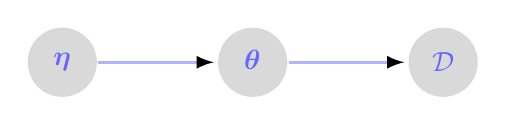
\begin{tikzpicture}[font=\sffamily,node distance=1.5cm,->,>=latex,auto,line width=0.4mm]
	
	\tikzset{node st/.style={state, draw=none,
			fill=gray!30!white,
			text=blue!60!white}}
	
	\node[node st] (I) {$\vec\eta$};
	\node[node st, right=of I] (G) {$\vec\theta$};
	\node[node st, right=of G] (S) {$\mathcal D$};  
	
	
	\draw[every loop,
	auto=right,
	draw=blue!30!white]
	(I) edge[->] node{} (G)
	(G) edge[->] node{} (S);
	
	\end{tikzpicture}
\end{center}

This is an example of a \green{hierarchical Bayesian model}, also called a \green{multi-level model}. 

\myspace
\p \blue{Bayesian Decision Theory} (5.7). Decision problems can be cast as games against nature, where natures selects a quantity $y \in \mathcal Y$ unknown to us, and then generates an observation $\vec x \in \mathcal X$ that we get to see. Our goal is to devise a \green{decision procedure} or \green{policy} $\delta : \mathcal X \mapsto \mathcal A$ for generating an action $a \in \mathcal A$ from observation $\vec x$ that's deemed most compatible with the hidden state $y$. We define ``compatible'' via a loss function $L(y, a)$:
\graybox{
	\delta(\vec x) 
		&= \argmin_{a \in \mathcal A} \rho(a \mid \vec x) \\
	\text{where}\quad
	\rho(a \mid \vec x)
		&= \E[p(y \mid \vec x)]{L(y, a)}
}
In this context, we call $\rho$ the \green{posterior expected loss}, and $\delta(x)$ the \green{Bayes estimator}. Some Bayes estimators for common loss functions are given below.
\begin{compactitem}
	\item \textbf{0-1 loss}: $L(y, a) = \ind\{ y \ne a \}$. Easy to show that $\delta(x) = \argmax_{y \in \mathcal Y} p(y \mid \vec x)$. 
\end{compactitem}


% <>~<>~<>~<>~<>~<>~<>~<>~<>~<>~<>~<>~<>~<>~<>~<>~<>~<>~<>~<>~<>~<>~<>~<>~<>~<>~<>~<>~<>~<>~<>~<>~<>~
\lecture{Machine Learning: A Probabilistic Perspective}{Linear Regression (Ch. 7)}{August 19, 2018}

\vspace{-1.7em}
{\scriptsize Kevin P. Murphy (2012). Linear Regression.\\ \textit{Machine Learning: A Probabilistic Perspective}.\\ }

\p \blue{Model Specification} (7.2). The linear regression model is a model of the form
\begin{align}
	p(y \mid \vec x, \vec\theta)
		&= \mathcal{N}(y \mid \vec{w}^T \vec x, \sigma^2)
\end{align}

\myspace
\p \blue{Maximum Likelihood Estimation} (least squares) (7.3). Most commonly, we'll estimate the parameters by computing the MLE, defined by
\begin{align}
	\hat{\vec{\theta}}
		&\triangleq \argmax_{\theta} \log p(\mathcal D \mid \vec\theta) \\
		&= \argmin_{\theta} \left[ - \log p(\mathcal D \mid \vec\theta) \right] \\
		&= - \inv{2\sigma^2} RSS(\vec w) - \frac{N}{2} \log(2\pi \sigma^2) \\
	RSS(\vec w)
		&\triangleq \sum_{i=1}^{N} (y_i - \vec{w}^T \vec[i]{x})^2
\end{align}
where $RSS(\vec w)$ is the \green{residual sum of squares}. Notice that $\vec\theta := (\vec w, \sigma^2)$, but typically we're focused on estimating $\vec w$\footnote{Since our goal is typically to make future predictions $\hat y(\vec x) = \vec{w}^T\vec{x}$, rather than sampling $y \sim p(y \mid \vec x, \vec\theta)$, we aren't concerned with estimating $\sigma^2$. We assume some variability, and the goal is focused on fitting the data to a straight line.}. 

\myspace
\p \blue{Derivation of the MLE} (7.3.1). We'll now denote the negative log likelihood as $\text{NLL}(\vec w)$ and drop constant terms that are irrelevant for the optimization task. 
\begin{align}
	\text{NLL}(\vec w)
		&= \onehalf || \vec y - \matr X \vec w ||_2^2
		= \onehalf \vec{w}^T (\matr{X}^T \matr{X}) \vec w - \vec{w}^T (\matr{X}^T \vec y) \\
	\text{where}\qquad
	\matr{X}^T\matr{X}
		&= \sum_{i=1}^{N} \vec[i]{x}\vec[i]{x}^T \\
	\matr{X}^T \vec y
		&= \sum_{i=1}^{N} \vec[i]{x} y_i
\end{align}

\Needspace{10\baselineskip}
And the optimal $\vec[OLS]{\hat w}$ be found by taking the gradient, setting to zero, and solving for $\vec w$ as usual:
\graybox{
	\nabla \text{NLL}(\vec w) 
		&= \matr{X}^T \matr X \vec w - \matr{X}^T \vec y \\
	\matr{X}^T \matr X \vec w 
		&= \matr{X}^T \vec y \qquad	\mtgreen{[normal eq.]} \\
	\vec[OLS]{\hat w}
		&= \left(  \matr{X}^T \matr X \right)^{-1} \matr{X}^T \vec y
}

\myspace
\p \blue{Geometric Interpretation} (7.3.2). Use the column-vector representation of $\matr X \in \R^{N \times D}$, where we assume $N > D$\footnote{This means we have more rows than columns, which means our column space cannot span all of $\R^N$.}. Our prediction can then be written
\begin{align}
	\hat{y} &= \matr{X} \vec w = w_1 \vec[1]{\tilde x} + \cdots + w_D \vec[D]{\tilde x}
\end{align}
i.e. a linear combination of the $D$ column vectors $\vec[i]{\tilde x} \in \R^{N}$. Crucially, observe that this means $\hat y \in \text{span}(\{ \vec{\tilde x} \}_i^D)$ no matter what (a hard constraint by definition of our model). So, how do you minimize the residual norm $||\vec y - \vec{\hat y}||$ given that $\vec{\hat y}$ is restricted to a particular subspace? You require $\vec y - \vec{\hat y}$ to be orthogonal to that subspace, of course\footnote{Consider that $\vec y - \hat{\vec y}$ points \textit{from} our prediction (which is in the constraint subspace) $\vec{\hat y}$ \textit{to} the true $\vec y$ that we want to get closest to. Intuitively that means $\vec{\hat y}$ is looking ``straight out'' at $\vec y$, in a direction orthogonal to the subspace that $\vec{\hat y}$ lives in. Formally, we can write $\vec y = (\vec[\parallel]{y}, \vec[\perp]{y})$, where $\vec[\parallel]{y}$ is the component within $\text{Col}(\vec x)$. The best we can do, then, is $\vec{\hat y} := \vec[\parallel]{y} $.}! Formally, this means $\vec[j]{\tilde x}^T ( \vec y - \vec{\hat y}) = 0$, for all $1 \le j \le D$. Equivalently,
\begin{align}
	\matr{X}^T(\vec y - \matr X \vec w) = \vec 0 \quad &\implies \quad \vec{\hat w} = (\matr{X}^T \matr X)^{-1} \matr{X}^T \vec y \\
	\vec{\hat y}
		&= \matr X \vec{\hat w} = \matr{P} \vec{y} \\
	\text{where}\qquad
	\matr P &\triangleq \matr X (\matr{X}^T \matr X)^{-1} \matr{X}^T 
\end{align}
Although this neat, I'm left unsatisfied since there appears to be no intuition of what the column vectors of $\matr X$ really mean on a conceptual level. 

\myspace
\p \blue{Robust Linear Regression} (7.4).\marginnote{Replacing Gaussian with heavy-tailed dists.}[2em] Gaussians sensitive to outliers, since their log-likelihood penalizes deviations quadratically\footnote{In other words, outliers initially get huge loss values, and the distribution shifts toward them to minimize loss (undesirably).}. One way to achieve \green{robustness} to outliers is to instead use a distribution with \green{heavy tails}, such that they still allow for higher likelihoods of outliers, but they don't need to shift the whole distribution around to accommodate for them. One popular choice is the \green{Laplace distribution},
\begin{align}
	p(y \mid \vec x , \vec w, b)
		&= \text{Lap}(y \mid \vec{w}^T \vec x, b)
		\triangleq \inv{2b} \exp\left\{ - \inv{b} | y - \vec{w}^T\vec x  | \right\} \\
	NLL(\vec w)
		&= \sum_i | y_i - \vec{w}^T \vec[i]{x} |
\end{align}
Goal: convert $NLL$ to a form easier to optimize (linear). Let $r_i \triangleq y_i - \vec{w}^T \vec[i]{x}$ be the i'th residual. The following steps show how we can convert this into a \green{linear program}:
\begin{align}
	r_i
		&\triangleq r_i^+ - r_i^- \qquad (r_i^+ \ge 0)(r_i^- \ge 0)     \\
	\min_{\vec w, \vec{r}^+, \vec{r}^-} \sum_i (r_i^+ + r_i^-)
	\qquad&\text{s.t.}\qquad \vec{w}^T\vec[i]{x} + r_i^+ - r_i^- = y_i \\
	\min_{\vec\theta} \vec{f}^T \vec{\theta}
	\qquad&\text{s.t.}\qquad \matr A \vec{\theta} \le \vec b, ~ \matr[eq]{A}\vec{\theta} = \vec[eq]{b}, ~ \vec 1 \le \vec\theta \le \vec u
\end{align}
where the last equation is the \green{standard form} of a LP. 

\myspace 
\p \blue{Ridge Regression} (7.5).\marginnote{Doing MAP instead of MLE}[2em] We know that MLE can overfit by essentially memorizing the data. If, for example, we model 21 points with a degree-14 polynomial\footnote{To review polynomials, search ``Lagrange interpolation'' in your CS 70 notes.}, we get many large positive and negative numbers for our learned coefficients, which allow the curve to wiggle in just the right way to almost perfectly interpolate the data -- \textbf{this is why we often regularize weights to have low absolute value}. This encourages smoother/less-wiggly curves. One way to do this is by using a zero-mean Gaussian prior on our weights:
\begin{align}
	p(\vec w)
		&= \prod_j \mathcal{N}(w_j \mid 0, \tau^2)
\end{align}
This makes our MAP estimation problem and solution take the form\marginnote{Note that $w_0$ is NOT regularized.}[2em]
\graybox{
	J(\vec w) 
		&= \inv{N} \sum_i^N \left(  y_i - \vec{w}^T \vec[i]{x} - w_0  \right) + \lambda ||\vec w||_2^2 \\
	\vec[ridge]{\hat w}
		&= ( \matr{X}^T \matr X + \lambda \matr[D]{I}  )^{-1} \matr{X}^T \vec y
}




% <>~<>~<>~<>~<>~<>~<>~<>~<>~<>~<>~<>~<>~<>~<>~<>~<>~<>~<>~<>~<>~<>~<>~<>~<>~<>~<>~<>~<>~<>~<>~<>~<>~
\lecture{Machine Learning: A Probabilistic Perspective}{Generalized Linear Models and the Exponential Family (Ch. 9)}{August 11, 2018}

\vspace{-1.7em}
{\scriptsize Kevin P. Murphy (2012). Generalized Linear Models and the Exponential Family.\\ \textit{Machine Learning: A Probabilistic Perspective}.\\ }

\p \blue{The Exponential Family} (9.2). Why is the exponential family important?
\begin{compactitem}
	\item It's the only family with \textbf{finite-sized sufficient statistics}\footnote{Given certain regularity conditions.}. 
	\item It's the only family for which \textbf{conjugate priors exist}.
	\item It makes the \textbf{least set of assumptions} subject to some user-chosen constraints.
	\item It's at the core of GLMs and variational inference. 
\end{compactitem}
\begin{definition}
	A pdf or pmf $p(\vec x \mid \vec\theta)$, for $\vec x \in \mathcal{X}^m$ and $\vec\theta \in \Theta \subseteq \R^d$, is said to be in the \green{exponential family} if it's of the form\marginnote{$h(\vec x)$ is a scaling constant, often 1.}[2em]
	\graybox{
		p(\vec x \mid \mgreen{\vec\theta})
			&= \inv{Z(\mgreen{\vec\theta})} h(\vec x) \exp\{ \mgreen{\vec\theta}^T \mpurple{\vec{\phi}(\vec x)} \}
			= h(\vec x) \exp\left\{ \mgreen{\vec\theta}^T \mpurple{\vec{\phi}(\vec x)} - A(\mgreen{\vec\theta})   \right\}	\\
		Z(\mgreen{\vec\theta})
			&= \int_{\mathcal{X}^m} h(\vec x) \exp\{\mgreen{\vec\theta}^T\mpurple{\vec{\phi}(\vec x)} \} \\
		A(\mgreen{\vec\theta})
			&= \log Z(\mgreen{\vec\theta}) 
	}
where $ \mgreen{\vec\theta}$ are the \green{natural (canonical) parameters}\footnote{We often generalize this with $\vec{\eta}(\vec\theta)$, which maps whatever params $\vec\theta$ we've chosen to the canonical params $\vec{\eta}(\vec\theta)$.}, and $\mpurple{\vec{\phi}(\vec x)}$ are the \purple{sufficient statistics}. 
\end{definition}
Below are some (quick/condensed) examples showing the first couple steps in rewriting familiar distributions in exponential family form:
\begin{align}
	\mtgreen{[Bernoulli]}&\quad \text{Ber}(x \mid \mu)
		= \mu^x (1 - \mu)^{1- x} = \exp\{  x \log \mu + (1 - x) \log(1- \mu)   \}  \\
	\mtgreen{[Multinoulli]}&\quad \text{Cat}(x \mid \vec\mu)
		= \prod_k^K \mu_k^{x_k} = \exp\left\{  \sum_k^{K-1} x_k \log\left(\mu_k/\mu_K \right) + \log\mu_K  \right\} 
\end{align}

\myspace
\p \blue{Log Partition Function} (9.2.3). The derivatives of the log partition, $A(\vec\theta)$, can be used to generate \green{cumulants}\footnote{The first and second cumulants are mean and variance.} for the sufficient statistics, $\vec{\phi}(\vec x)$. 
\begin{align}
	\pderiv{A(\vec\theta)}{\vec\theta} &= \E{\vec{\phi}(\vec x)} \\
	\nabla^2 A(\vec\theta) &= \text{cov}\left[ \vec{\phi}(\vec x) \right]
\end{align}


\myspace
\p \blue{MLE for the Exponential Family} (9.2.4). The likelihood takes the form\marginnote{It appears that we are denoting $1/Z$ with $g$ now.}[3em]
\begin{align}
	p(\mathcal D \mid \vec\theta)
		&= \left[ \prod_i^N h(\vec{x}^{(i)}) \right] g(\vec\theta)^N \exp\left\{ \vec{\eta}(\vec\theta)^T \vec{\phi}(\mathcal D) \right\} \\
	\vec{\phi}(\mathcal D) 
		&=  \sum_i^N \vec{\phi}(\vec{x}^{(i)}) 
		= \begin{bmatrix} \sum_i \phi_1 & \cdots & \sum_i \phi_K  \end{bmatrix}
\end{align}
where I've denoted $\sum_{i=1}^N \phi_k(\vec{x}^{(i)})$ as simply $\sum_i \phi_k$. The \green{Pitman-Koopman-Darmois theorem} states, given certain regularity conditions/constraints\footnote{The wording is weird here. We mean ``out of all families/distributions that \textit{already} satisfy certain constraints that must be met, the exponential family is the only...''. For example, the uniform distribution has finite statistics and is not in the exponential family, but it does not meet the constraint that its support must be independent of the parameters, so it's outside the scope of the theorem.}, that the exponential family is the only family with \textit{finite sufficient statistics} (dimensionality independent of the size of the data set). For example, in the above formula, we have $K + 1$ sufficient statistics ($+1$ since we need to know the value of $N$). \\

\p Consider a canonical\footnote{Defined as those which satisfy $\vec{\eta}(\vec\theta) = \vec\theta$.} exponential family which also sets $h(\cdot) = 1$. The log-likelihood is
\begin{align}
	p(\mathcal D \mid \vec\theta)
		&= \vec\theta^T \vec{\phi}(\mathcal D) - N A (\vec\theta)
\end{align}
Since $-A(\vec\theta)$ is concave\footnote{We know $-A$ is concave because $A$ is convex. We know $A$ is convex because $\nabla^2 A$ is positive definite. Remember that any twice-differentiable multivariate function $f$ is convex IFF its Hessian is pd for all $\vec\theta$. See sec 7.3.3 and 9.2.3 for more.} and the other term is linear in $\vec\theta$, the log-likelihood is concave and thus has a global maximum.

\myspace
\p \blue{Maximum Entropy Derivation of the Exponential Family} (9.2.6). Suppose we don't know which distribution $p$ to use, but we do know the expected values of certain features or functions:
\begin{align}
	F_k \triangleq \E[\vec x \sim p(\rvec x)]{f_k(\vec x)} = \sum_{\vec x} f_k(\vec x) p(\vec x)
\end{align}
The principle of \green{maximum entropy} or \green{maxent} says we should pick the distribution with maximum entropy, subject to the constraints that the moments of the distribution match the empirical moments of the specified functions $f_k(\vec x)$. Treating $p$ as a fixed length vector (i.e. assuming $\vec x$ is discrete), we can take the derivative of our Lagrangian (entropy in units of nats with constraints) w.r.t. each ``element'' $p_x = p(\vec x)$ to find the optimal distribution.
\begin{align}
	J(p, \vec\lambda)
		&= H(p) + \lambda_0 \left( 1 - \sum_{\vec x} p(\vec x) \right) + \sum_k \lambda_k \left(F_k - \sum_{\vec x} p(\vec x) f_k(\vec x) \right) \\
	\pderiv{J}{p(\vec x)}
		&= -1 - \log p(\vec x) - \lambda_0 - \sum_k \lambda_k f_k(\vec x)
\end{align}
Setting this derivative to zero yields
\begin{align}
	p(\vec x) 
		&= \inv{Z} \exp\left\{ -\sum_k \lambda_k f_k(\vec x)  \right\}
\end{align}
Thus the maxent distribution $p(\vec x)$ has the form of the exponential family, a.k.a. the \green{Gibbs distribution}. 











% <>~<>~<>~<>~<>~<>~<>~<>~<>~<>~<>~<>~<>~<>~<>~<>~<>~<>~<>~<>~<>~<>~<>~<>~<>~<>~<>~<>~<>~<>~<>~<>~<>~
\lecture{Machine Learning: A Probabilistic Perspective}{Mixture Models and the EM Algorithm (Ch. 11)}{August 26, 2018}

\vspace{-1.7em}
{\scriptsize Kevin P. Murphy (2012). Mixture Models and the EM Algorithm.\\ \textit{Machine Learning: A Probabilistic Perspective}.\\ }

\p \blue{Latent Variable Models} (LVMs) (11.1). In this chapter, we explore directed GMs that have hidden/latent variables. Advantages of LVMs:
\begin{compactenum}
	\item Often have fewer params.
	\item Hidden vars can serve as a bottleneck (representation learning).
\end{compactenum}

\myspace
\p \blue{Mixture Models} (11.2). The simplest form of LVM is where the hidden variables $z_i \in \{1, \ldots, K\}$ represent a discrete latent state. We use discrete prior $p(z_i) = \text{Cat}(\vec\pi) = \pi_i$, and likelihood $p(\vec[i]{x} \mid z{=}k) = p_k(\vec[i]{x})$. A \green{mixture model} is defined by\marginnote{We call $p_k$ the $k$th \textbf{base distribution}.}[2em]
\graybox{
	p(\vec[i]{x} \mid \vec\theta)
		&= \sum_{k=1}^{K} \pi_k p_k(\vec[i]{x} \mid \vec\theta)	
}
Some popular mixture models:
\begin{compactitem}
	\item \green{Mixture of Gaussians} (11.2.1). Each $p_k = \mathcal{N}(\vec[k]{\mu}, \matr[k]{\Sigma})$. Given large enough $K$, \textit{a GMM can approximate any density defined on $\R^D$.}
	
	\item \green{Mixture of Multinoullis} (11.2.2). Let $\vec x \in \{0, 1\}^D$. Each $p_k(\vec x) = \prod_j^D \text{Ber}(x_j \mid \mu_{jk})$. Below, I derive the expectation and covariance of $\vec x$ in this case\footnote{Shown in excruciating detail because I was unable to work through this in my head alone.}. 
	\begin{align}
		\E{\rvec x}
			&= \sum_{\vec x} \vec{x} p(\vec x) \\
			&= \sum_{\vec x} \vec{x} \sum_k^K \pi_k p_k(\vec x) \\
			&= \sum_{\vec x} \vec{x} \sum_k^K \pi_k \prod_{j}^{D} \text{Ber}(x_j\mid \mu_{jk}) \\
			&= \sum_k^{D} \pi_k \sum_{x_1} \cdots \sum_{x_D} \vec x \prod_j^D \text{Ber}(x_j\mid \mu_{jk}) \\
			&= \sum_k^{D} \pi_k \sum_{x_1} \text{Ber}(x_1 \mid \mu_{1k}) \cdots \sum_{x_D} \text{Ber}(x_D \mid \mu_{Dk}) \vec x \\
			&= \sum_k^{D} \pi_k \vec[k]{\mu} 
	\end{align}
	Next we want to find $\text{cov}(\rvec x) = \E{\rvec{x}\rvec{x}^T} - \E{\rvec x}\E{\rvec{x}}^T$. I think the insight that makes finding the first term easiest is realizing that you only need to find the two cases, $\E{x_i^2}$ and $\E{x_i x_{j\ne i}}$, where in this case
	\begin{align}
		\E{x_i^2} &= \sum_k \pi_k \mu_{ik} \\
		\E{x_i x_{j \ne i}} &= \sum_k \pi_k \mu_{ik} \mu_{jk} \\
		\therefore \E{\rvec x \rvec{x}^T}
			&= \sum_k \pi_k \left( \matr[k]{\Sigma} + \vec[k]{\mu} \vec[k]{\mu}^T  \right)
	\end{align}
	where $\Sigma_k = \text{diag}(\mu_{jk}(1- \mu_{jk}))$ is the covariance of $\vec x$ under $p_k$. The fact that the mixture covariance matrix is now non-diagonal confirms that the mixture can capture correlations between variables $x_i, x_{j\ne i}$, unlike a single product-of-Bernoullis model.
	
\end{compactitem}

\myspace
\p \blue{The EM Algorithm} (11.4). In LVMs, it's usually intractable to compute the MLE since we have to marginalize over hidden variables while satisfying constraints like positive definite covariance matrices, etc. The EM algorithm gets around these issues via a two-step process. The first step involves taking an expectation, where the expectation is over $\vec z \sim p(\vec z \mid \vec x, \theta^{t-1})$ for each individual observed $\vec x$, where we use the current parameter estimates when sampling $\vec z$ in the expectation. \textbf{This gives us an auxiliary likelihood that's a function of $\vec\theta$} which will serve as a stand-in (in the 2nd step) for what we typically use as the likelihood in MLE. The second step is then just finding the optimal $\vec{\theta}^t$ over the auxiliary likelihood function from the first step. This iterates until convergence or some stopping condition.

\begin{algorithm}[Procedure: EM Algorithm]

First, let's define our auxiliary function $Q$ as
	\begin{align}
		Q(\vec\theta \mid \vec{\theta}^{t-1})
			&= \E[p(\vec z \mid \vec x, \vec{\theta}^{t-1})]{\ell_c(\vec\theta) \mid \mathcal{D}} \\
		\text{where}\quad
		\ell_c(\vec\theta)
			&= \sum_{i=1}^{N} \log p(\vec{x}^{(i)}, \vec{z}^{(i)} \mid \vec\theta)
	\end{align}
	where, again, the ``expectation'' serves the purpose of determining the expected value of $\vec{z}^{(i)}$ for each observed $\vec{x}^{(i)}$. It's somewhat of a misnomer to denote the expectation like this, since each $\vec{z}^{(i)}$ is innately tied with its corresponding observation $\vec{x}^{(i)}$.
	
	\begin{compactenum}
		\item \textbf{E-Step}: Evaluate $Q(\vec\theta \mid \vec{\theta}^{t-1})$ using (obviously) the previous parameters $\vec{\theta}^{t-1}$. This yields a function of $\vec\theta$. This gives us the expected log-likelihood function of $\vec\theta$ for the observed data $\mathcal D$. 
		
		\item \textbf{M-Step}: Optimize $Q$ w.r.t $\vec\theta$ to get $\vec{\theta}^t$:
		\begin{align}
			\vec{\theta}^t 
				&= \argmax_{\vec\theta} Q(\vec\theta \mid \vec{\theta}^{t-1})
		\end{align}
	\end{compactenum}

\end{algorithm}








% <>~<>~<>~<>~<>~<>~<>~<>~<>~<>~<>~<>~<>~<>~<>~<>~<>~<>~<>~<>~<>~<>~<>~<>~<>~<>~<>~<>~<>~<>~<>~<>~<>~
\lecture{Machine Learning: A Probabilistic Perspective}{Latent Linear Models (Ch. 12)}{September 14, 2018}

\vspace{-1.7em}
{\scriptsize Kevin P. Murphy (2012). Latent Linear Models.\\ \textit{Machine Learning: A Probabilistic Perspective}.\\ }

\p \blue{Factor Analysis} (12.1). Whereas mixture models define $p(z) = \text{Cat}(\vec\pi)$ for a single hidden variable $z \in \{1, \ldots, K\}$, \green{factor analysis} begins by instead using a \textit{vector} of \textit{real-valued} latent variables, $\vec z \in \R^{L}$. The simplest prior is $\vec z \sim \mathcal{N}(\vec[0]{\mu}, \matr[0]{\Sigma})$. If $\vec x \in \R^D$, we can define
\begin{align}
	p(\vec[i]{x}\mid \vec[i]{z}, \vec\theta)
		&= \mathcal{N}(\matr W \vec[i]{z} + \vec\mu, \matr\Psi)
\end{align}
where
\begin{compactitem}
	\item $\matr W \in \R^{D \times L}$: \green{factor loading matrix}.
	
	\item $\matr\Psi \in \R^{D \times D}$ is a \underline{diagonal} covariance matrix, since we want to ``force'' $\vec{z}$ to explain the correlation\footnote{It's easier to think of this graphically. Our model asserts that $\vec[i]{x} \perp \vec[j\ne i]{x} \mid \vec{z}$. Independence implies zero correlation, and we cement this by constraining $\matr\Psi$ to be diagonal. See your related note on LFMs, chapter 13 of the DL book.}. If $\matr\Psi  = \sigma^2 \matr I$, we get \green{probabilistic PCA}. 
\end{compactitem}
Summaries of key points regarding FA:
\begin{compactitem}
	\item \textbf{Low-rank parameterization of MVN}. FA can be thought of as specifying $p(\vec x)$ using a small number of parameters. [math] yields that
	$$
	\text{cov}(\vec x) = \matr W \matr{W}^T + \matr\Psi
	$$
	which has $\mathcal{O}(LD)$ params (remember $\matr\Psi$ is diagonal) instead of the usual $\mathcal{O}(D^2)$. 
	
	\item \textbf{Unidentifiability}: The params of an FA model are unidentifiable. 
\end{compactitem}

\myspace
\p \blue{Classical PCA} (12.2.1). Goal: find an orthogonal set of $L$ linear basis vectors $\vec[j]{w} \in \R^D$, and the scores $\vec[i]{z} \in \R^L$, such that we minimize the average \green{reconstruction error}:
\begin{align}
	J(\matr W, \matr Z)
		&= \inv{N} \sum_{i=1}^{N} || \vec[i]{x} - \vec[i]{\hat x} ||^2, 
		\quad\text{where}\quad
		\vec[i]{\hat x} := \matr W \vec[i]{z} \\
		&= || \matr X - \matr W \matr{Z}^T ||_F^2
\end{align}
where $\matr W \in \R^{D \times L}$ is orthonormal. \textbf{Solution}: assign each column $\matr[:,\ell]{W}$ to the eigenvector with $\ell$'th largest eigenvalue of $\matr{\hat \Sigma} = \inv{N} \sum_i^N \vec[i]{x}\vec[i]{x}^T$, assuming $\E{\vec x} = \vec{0}$. Then we compute $\vec[i]{\hat z} := \matr{W}^T \vec[i]{x}$. 

\begin{example}[Proof: PCA]
	\textbf{Case: L=1}. Goal: Find the best 1-d solution, $\vec{w} \in \R^D$, $z_i \in \R$, $\vec z \in \R^N$. Remember that $||\vec w||_2 = 1$. 
	\begin{align}
		J(\vec w, \vec{z})
			&= \inv{N} \sum_i^N || \vec[i]{x} - z_i \vec{w} ||^2 
			= \inv{N} \left[   \vec[i]{x}^T \vec[i]{x} - 2 z_i \vec{w}^T \vec[i]{x} + z_i^2  \right] \\
		\pderiv{J}{z_i}
			&= 0 \quad\rightarrow\quad z_i = \vec{w}^T\vec[i]{x} \\
		J(\vec w)
			&= \inv{N}\sum_i^N \left[ \vec[i]{x}^T\vec[i]{x} - z_i^2 \right]
			= \text{const} - \inv{N} \sum_i^N z_i^2 \\
		\therefore
		\argmin_{\vec w} J(\vec w) 
			&= \argmax_{\vec w} \text{Var}\left[  \vec{\tilde z} \right]
	\end{align}
	This shows why PCA finds directions of maximal variance -- aka the \purple{analysis view} of PCA. Before finding the optimal $\vec w$, don't forget the Lagrange multipliers for constraining unit norm,
	\begin{align}
		\tilde{J}(\vec w)
			&= \vec{w}^T \matr{\hat \Sigma} \vec{w} + \lambda (\vec{w}^T \vec w - 1)
	\end{align}
\end{example}

\myspace
\p \blue{Singular Value Decomposition} (SVD) (12.2.3). Any real $N \times D$ matrix $\matr X$ can be decomposed as
\begin{align}
	\matr X
		&= \underbrace{\matr U}_{N \times N} \underbrace{\matr S}_{N \times D} \underbrace{\matr{V}^T}_{D \times D}
\end{align}
where the columns of $\matr U$ are the left singular vectors, and the columns of $\matr V$ are the right singular vectors. \textbf{Economy-sized SVD} will shrink $\matr U$ to be $N \times D$ and $\matr S$ to be $D \times D$ (we're assuming N > D). 




% <>~<>~<>~<>~<>~<>~<>~<>~<>~<>~<>~<>~<>~<>~<>~<>~<>~<>~<>~<>~<>~<>~<>~<>~<>~<>~<>~<>~<>~<>~<>~<>~<>~
\lecture{Machine Learning: A Probabilistic Perspective}{Markov and Hidden Markov Models (Ch. 17)}{August 11, 2018}

\vspace{-1.7em}
{\scriptsize Kevin P. Murphy (2012). Markov and Hidden Markov Models.\\ \textit{Machine Learning: A Probabilistic Perspective}.\\ }

\p \blue{Hidden Markov Models} (17.3). HMMs model a joint distribution over a sequence of $T$ observations $\slice[T]{x}$ and hidden states $\slice[T]{z}$,
\begin{align}
	p(\slice[T]{z}, \slice[T]{x})
		&= p(\slice[T]{z}) p(\slice[T]{x} \mid \slice[T]{z})
		= \left[ p(z_1) \prod_{t=2}^{T} p(z_t \mid z_{t-1})  \right]
			\left[ \prod_{t=1}^T p(\vec[t]{x} \mid z_t) \right]
\end{align}
where each hidden state is discrete: $z_t \in \{1, \ldots, K \}$, while each observation $\vec[t]{x}$ can be discrete or continuous.

\myspace
\p \blue{The Forwards Algorithm} (17.4.2). Goal: compute the filtered\footnote{They're called ``filtered'' because they use all observations $\slice[t]{x}$ instead of just $\vec[t]{x}$, which reduces/filters out the noise more.} marginals $p(z_t \mid \slice[t]{x})$.
\begin{compactenum}
	\item \textbf{Prediction step}. Compute the \textit{one-step-ahead predictive density} $p(z_t \mid \slice[t-1]{x})$,
	\begin{align}
		p(z_t {=} j \mid \slice[t-1]{x})
			&= \sum_i p(z_t = j, z_{t-1} = i \mid \slice[t-1]{x}) 
	\end{align}
	which will serve as our prior for time $t$ (since it does not take into account observed data at time t). 
	
	\item \textbf{Update step}. We ``update'' our beliefs by observing $\vec[t]{x}$,
	\begin{align}
		\alpha_t(j)
			&\triangleq p(z_t {=} j \mid \slice[t]{x}) \\
			&= \frac{  p(z_t {=} j, \vec[t]{x}, \slice[t-1]{x}) }{  p(\slice[t]{x}) } \\
			&= \frac{ \cancel{ p(\slice[t-1]{x}) } p(z_t{=}j \mid \slice[t-1]{x}) p(\vec[t]{x} \mid z_t {=} j, \cancel{ \slice[t-1]{x}  }) }{
				\cancel{  p(\slice[t-1]{x}) } p(\vec[t]{x} \mid \slice[t-1]{x}) } \\
			&= \inv{Z_t} p(z_t {=} j \mid \slice[t-1]{x}) p(\vec[t]{x} \mid z_t {=} j)
	\end{align}
\end{compactenum}
Notice that we can also use the values of $Z_t$ to compute the log probability of the evidence:
\begin{align}
	\log p(\slice[T]{x} \mid \vec\theta)
		&= \sum_{t=1}^{T} \log p(\vec[t]{x} \mid \slice[t-1]{x}) 
		= \sum_{t=1}^T \log Z_t
\end{align}

\begin{algorithm}[Forwards Algorithm (Algorithm 17.1)]
	We are given transition matrix $T_{i,j} = p(z_t = j \mid z_{t-1} = i)$, evidence vectors $\psi_t(j) = p(\vec[t]{x} \mid z_t{=}j)$, and initial state distribution $\pi(j) = p(z_1 = j)$. 
	
	\begin{compactenum}
		\item First, compute the initial $[\alpha_1, Z_1] = \text{normalize}(\psi_1 \odot \pi)$. 
		
		\item For time $2 \le t \le T$, compute $[\alpha_t, Z_t] = \text{normalize}(\psi_t \odot \matr{T}^T \vec[t-1]{\alpha})$. 
		
		\item Return $\slice[T]{\alpha}$ and $\log p(\slice[T]{x}) = \sum_t \log Z_t$. 
	\end{compactenum} 
\end{algorithm}

\myspace
\p \blue{The Forwards-Backwards Algorithm} (17.4.3). Goal: compute the smoothed marginals, $p(z_t = j \mid \slice[T]{x})$. 
\begin{align}
	\gamma_t(j)
		&\triangleq p(z_t = j \mid \slice[T]{x})   \\
		&\propto p(z_t = j \mid \slice[t]{x}) p(\slice[T][t+1]{x} \mid z_t = j) \\
		&= \alpha_t(j) \beta_t(j) \\
	\text{where}\quad
	\beta_t(j)
		&\triangleq p(\slice[T][t+1]{x} \mid z_t {=} j)  \\
		&= p(\vec[t+1]{x}, \slice[T][t+2]{x} \mid z_t{=}j ) \\
		&= \sum_{i} p(z_{t+1}{=}i, \vec[t+1]{x}, \slice[T][t+2]{x} \mid z_t{=}j ) \\
		&= \sum_i p(z_{t+1}{=}i, \vec[t+1]{x} \mid z_t{=}j) p(\slice[T][t+2]{x} \mid \cancel{z_t{=}j}, z_{t+1}{=}i, \cancel{\vec[t+1]{x}} ) \\
		&= \sum_i p(z_{t+1}{=}i \mid z_t{=}j) p(\vec[t+1]{x} \mid z_{t+1}{=}i) p(\slice[T][t+2]{x} \mid z_{t+1}{=}i) \\
		&=  \sum_i p(z_{t+1}{=}i \mid z_t{=}j) p(\vec[t+1]{x} \mid z_{t+1}{=}i) \beta_{t+1}(i)
\end{align}
Using the same notation as Algorithm 17.1 above, the matrix-vector form for $\beta$ is
\begin{align}
	\vec[t]{\beta} &= \matr{T} \left( \vec[t]{\psi} \odot \vec[t+1]{\beta}  \right)
\end{align}
with base case $\vec[T]{\beta} = \vec{1}$. 

\myspace
\p \blue{The Viterbi Algorithm} (17.4.4). Denote the [probability for] the most probable path leading to $z_t{=}j$ as\marginnote{It is common to work in the log-domain when computing $\delta$.}[2em]
\begin{align}
	\delta_t(j) 
		&\triangleq \max_{\slice[t-1]{z}} p(\slice[t-1]{z}, z_t{=}j \mid \slice[t]{x}) \\
		&= \max_i \delta_{t-1}(i) \cdot T_{i,j} \cdot  \psi_t(j)
\end{align}
with initialization of $\delta_1(j) = \pi_j \psi_1(j)$. We compute this until termination at $z_{T}^* = \argmax_i \delta_T(i)$. Note the $\argmax$ here instead of a $\max$ -- we keep track of both for all time steps. We do this so we can perform \green{traceback} to get the full most probable state sequence, starting at $T$ and ending at $t=1$:
\begin{align}
	z_t^* &= a_{t+1}(z_{t+1}^*)
\end{align}
where $a_t(j)$, the most probable state at time $t-1$ leading to state $j$ at time $t$, is the same formula as $\delta_t(j)$ but with an $\argmax$. 






























% <>~<>~<>~<>~<>~<>~<>~<>~<>~<>~<>~<>~<>~<>~<>~<>~<>~<>~<>~<>~<>~<>~<>~<>~<>~<>~<>~<>~<>~<>~<>~<>~<>~
\lecture{Machine Learning: A Probabilistic Perspective}{Undirected Graphical Models (Ch. 19)}{August 11, 2018}

\vspace{-1.7em}
{\scriptsize Kevin P. Murphy (2012). Undirected Graphical Models.\\ \textit{Machine Learning: A Probabilistic Perspective}.\\ }

\p \blue{Learning} (19.5). Consider a MRF in log-linear form over $C$ cliques and its log-likelihood (scaled by 1/N):
\begin{align}
	p(\vec y \mid \vec\theta)	
		&= \inv{Z(\vec\theta)} \exp\left\{ \sum_c \vec[c]{\theta}^T \vec[c]{\phi}(\vec y)  \right\} \\
	\ell(\vec\theta)
		&= \inv{N} \sum_i \left[ \sum_c  \vec[c]{\theta}^T \vec[c]{\phi}(\vec[i]{y}) - \log Z(\vec\theta)    \right]
\end{align}
We know from chapter 9 that this log-likelihood is concave in $\vec\theta$, and that $\pderiv{}{\vec[c]{\theta}} \log Z = \E{\phi_c}$. So the gradient of the LL is
\begin{align}
	\pderiv{\ell}{\vec[c]{\theta}} 
		&= \left[ \inv{N} \sum_i \vec[c]{\phi}(\vec[i]{y}) \right] - \E[p(\vec y \mid \vec\theta)]{\vec[c]{\phi}(\vec y)}
\end{align}
Note that the first (``clamped'') term only needs to be computed once for any $\vec[i]{y}$, it is completely independent of any parameters. It's just evaluating feature functions, which e.g. for CRFs are often all indicator functions.

\myspace
\p \blue{CRF Training} (19.6.3). For [linear-chain] CRFs, the equations change slightly (but importantly).
\begin{align}
	\ell(\vec w)
		&\triangleq \inv{N} \sum_i \left[ \sum_c \vec[c]{w}^T \vec[c]{\phi}(\vec[i]{y}, \vec[i]{x}) - \log Z(\vec w, \vec[i]{x}) \right] \\
	\pderiv{\ell}{\vec[c]{w}}
		&= \inv{N} \sum_i \left[
			\vec[c]{\phi}(\vec[i]{y}, \vec[i]{x}) 
		- \E[ p( \vec{y} \mid  \bm{x}_i ) ]{ \vec[c]{\phi}(\vec[i]{y}, \vec[i]{x}) }		
		\right]
\end{align}
It's important to recognize that the gradient of the log partition function now must be computed for \textit{each} instance $\vec[i]{x}$. 





\begin{comment}
% <>~<>~<>~<>~<>~<>~<>~<>~<>~<>~<>~<>~<>~<>~<>~<>~<>~<>~<>~<>~<>~<>~<>~<>~<>~<>~<>~<>~<>~<>~<>~<>~<>~
\lecture{Machine Learning: A Probabilistic Perspective}{Variational Inference (Ch. 21)}{August 12, 2018}

\vspace{-1.7em}
{\scriptsize Kevin P. Murphy (2012). Variational Inference.\\ \textit{Machine Learning: A Probabilistic Perspective}.\\ }
\end{comment}








% ==================================================================================
% ==================================================================================
% ==================================================================================
% Convex Optimization
% ==================================================================================
% ==================================================================================
% ==================================================================================
\mysection{Convex Optimization}\label{Convex Optimization}

\newcommand{\relint}{\rvec{relint}}
\newcommand{\aff}{\rvec{aff}}
\newcommand{\conv}{\rvec{conv}}

% ======================================================================================
\lecture{Convex Optimization}{Convex Sets (Ch. 2)}{August 19, 2018}
% ======================================================================================
\vspace{-1.7em}
{\scriptsize Boyd and Vandenberghe (2004). Convex Sets.\\ \textit{Convex Optimization}.\\ }


\begin{definition}[-1em][Lines and line segments]
	Viewed as a function of $\theta \in \R$, we can express the equation for a \green{line} in $\R^n$ in the following two ways:
	\begin{align}
		y &= \theta x_1 + (1 - \theta) x_2 \\
		y &= x_2 + \theta (x_1 - x_2)
	\end{align}
	for some $x_1, x_2{\ne}x_1 \in \R^n$. If we restrict $\theta \in [0, 1]$, we have a \green{line segment}. 
\end{definition}

\begin{definition}[-1em][Affine sets]
	A set $C \subseteq \R^n$ is \green{affine} if the \textit{line} (not just segment) through any two distinct points in $C$ also lies in $C$. More generally, this implies that for any set of points $\{x_1, \ldots, x_k\}$, with each $x_i \in C$, all \green{affine combinations},
	\begin{align}
		\sum_{i=1}^{k} \theta_i x_i, \quad\text{where}\quad \sum_i \theta_i = 1
	\end{align}
	are in $C$, too. Related terminology:
	\begin{compactitem}
		\item \green{affine hull} of any set $C \subseteq \R^n$, denoted $\rvec{aff}C$, is the set of all affine combinations of points in $C$. 
		
		\item \green{affine dimension} of a set $C$ is the dimension of its affine hull. 
		
		\item \green{relative interior} of a set $C$, denoted $\rvec{relint}C$, is its interior\footnote{
			The \purple{interior of a set} $C \subseteq \R^n$, denoted $\rvec{int}C$, is the set of all points interior to $C$. A point $x \in C$ is interior to $C$ if $\exists \epsilon > 0$ for which \textit{all points} in the set
			$$
			\{ y \in R^n \mid ||y - x||_2 \le \epsilon  \}
			$$
			are also in $C$.
		}
		relative to $\rvec{aff}C$,
		\begin{align}
			\rvec{relint}C
				&\triangleq \{  x \in C \mid B(x, r) \cap \aff C \subseteq C  ~\text{for some}~ r > 0  \}
		\end{align}
	\end{compactitem}
\end{definition}
There's a lot of neat things to say here, but I only have space to state the results:
\begin{compactitem}
	\item If $C$ is an affine set and $x_0 \in C$, then
	\begin{align}
		V = C - x_0 \triangleq \{ x - x_0 \mid x \in C  \}
	\end{align}
	is a \textit{subspace}, i.e. closed under sums and scalar multiplication. 
	
	\item The solution set of a system of linear equations, $C = \{ x \mid Ax=b  \}$, is an affine set. The subspace associated with $C$ is the \textit{nullspace} of $A$. 
\end{compactitem}


\begin{definition}[-1em][Convex sets]
	A set $C$ is \green{convex} if it contains all \green{convex combinations},
	\begin{align}
		\sum_{i=1}^{k} \theta_i x_i, \quad\text{where}\quad \sum_i \theta_i = 1, ~\text{and}~ \theta_i \ge 0
	\end{align}
	Related terminology:
	\begin{compactitem}
		\item \green{convex hull} a set $C$, denoted $\conv C$, is the set of all convex combinations of points in $C$. 
	\end{compactitem}
\end{definition}


\begin{definition}[-1em][Cones]
	A set $C$ is called a \green{cone} if $(\forall x \in C)(\theta \ge 0)$ we have $\theta x \in C$. A set $C$ is called a \green{convex cone} if it contains all \green{conic combinations},
	\begin{align}
		\sum_{i=1}^{k} \theta_i x_i, \quad\text{where}\quad \theta_i \ge 0
	\end{align}
	of points in $C$. Related terminology:
	\begin{compactitem}
		\item \green{conic hull} of a set $C$ is the set of all conic combinations of points in $C$.
	\end{compactitem}
\end{definition}





















% ==================================================================================
% ==================================================================================
% ==================================================================================
% BDA
% ==================================================================================
% ==================================================================================
% ==================================================================================
\mysection{Bayesian Data Analysis}\label{Bayesian Data Analysis}


% ======================================================================================
\lecture{Bayesian Data Analysis}{Probability and Inference (Ch. 1)}{November 22, 2017}
% ======================================================================================

\p The process of Bayesian Data Analysis can be divided into the following 3 steps:
\begin{compactenum}
	\item Setting up a \textit{full probability model}.
	\item Conditioning on observed data. Calculating the \textit{posterior distribution} over unobserved quantities, given observed data.
	\item Evaluating the fit of the model and implications of the posterior. 
\end{compactenum}
\textbf{Notation}: In general, we let $\theta$ denote unobservable vector quantities or population \textit{parameters} of interest, and $y$ as collected data. This means our \textit{posterior} takes the form $p(\theta \mid y)$, and our \textit{likelihood} takes the form $p(y \mid \theta)$. 

\myspace
\p \blue{Means and Variances of Conditional Distributions}.
\graybox{
		\E{u} &= \E[v]{\E[u]{u \mid v}} \\
		\Var{u} &= \E[v]{ \Var{u \mid v} } + \Var{ \E[u]{u \mid v} }
}
\begin{example}[Proofs]
\vspace{-1em}
\begin{align}
	\E{u} 
		&= \int \mathrm{d}v \Prob{v} \int \mathrm{d}u \Prob{u \mid v} \\
		&= \E[v]{\E[u]{u \mid v}} \\
	\Var{u}
		&= \E{u^2} - \E{u}^2 \\
		&= \E[v]{ \E[u]{u^2 \mid v} } - \E[v]{\E[u]{u \mid v}}^2 \\
		&= \E[v]{ \E[u]{u^2 \mid v} - \E[u]{u \mid v}^2 } + \E[v]{\E[u]{u \mid v}^2} - \E[v]{\E[u]{u \mid v}}^2 \\
		&= \E[v]{ \Var{u \mid v} } + \Var{ \E[u]{u \mid v} }
\end{align}
\end{example}

\myspace
\p \blue{Transformation of Variables}. 
\begin{align}
	\Prob[v]{v} &= |J| \Prob[u]{f^{-1}(v)}
\end{align}
where $u$ and $v$ have the same dimensionality, and $|J|$ is the determinant of the Jacobian of the transformation $u = f^{-1}(v)$. When working with parameters defined on the open unit interval, $(0, 1)$, we often use the logistic transformation:\marginnote{
	$J_{i,j} = \pderiv{u}{v} = \pderiv{f^{-1}(v)}{v}$
}[-4em]
\begin{align}
	\text{logit}(u) &= \log\left(  \frac{u}{1 - u} \right) \\
	\text{logit}^{-1}(v) &= \log\left(  \frac{e^v}{1 + e^{v} } \right) 
\end{align}

\myspace
\p \blue{Standard Probability Distributions}\footnote{The \green{gamma function}, $\Gamma(x)$, is defined as 
	\begin{align}
		\Gamma(x) &= \int_0^\infty t^{x - 1} e^{-t} \mathrm{d}t
	\end{align}
or simply as $(x - 1)!$ if $x \in \mathbb{Z}^+$. }. 
\begin{table*}[h!]
	\centering
	\begin{tabular}{l l l}
		\toprule
		Distribution & Notation & Density Function \\ \midrule
		Beta & Beta$(\alpha, \beta)$ & $p(\theta) = \tfrac{\Gamma(\alpha + \beta)}{ \Gamma(\alpha)\Gamma(\beta) } \theta^{\alpha - 1}(1 - \theta)^{\beta -1}$  \\ 
		Inverse-gamma & $\text{Inv-gamma}(\alpha, \beta)$	& $p(\theta) = \tfrac{\beta^\alpha}{\Gamma(\alpha)}\theta^{-(\alpha + 1)} e^{-\beta/\theta}  $   \\	
		Normal (univariate) & N($\mu, \sigma^2$) & $p(\theta) = \inv{\sqrt{2 \pi \sigma}} \exp\big( - \inv{2\sigma^2} (\theta - \mu)^2  \big)$ \\
		Scaled inverse-$\chi^2$ & Inv-$\chi^2(\nu, s^2)$  &  $\theta \sim \text{Inv-gamma}(\tfrac{\nu}{2}, \tfrac{\nu}{2}s^2)$ \\
		\bottomrule
	\end{tabular}
	\label{table:distributions}
\end{table*}



% ======================================================================================
\lecture{Bayesian Data Analysis}{Single-Parameter Models (Ch. 2)}{November 22, 2017}
% ======================================================================================

\p Since we'll be referring to the binomial model frequently, below are the main distributions for reference:
\begin{align}
	p(y \mid \theta) &= Bin(y \mid n, \theta) = \binom{n}{y} \theta^y (1 - \theta)^{n - y} \\
	p(\theta \mid y) &\propto \theta^y (1 - \theta)^{n - y} \\
	\theta \mid y &\sim \text{Beta}(y + 1, n - y + 1) 
\end{align}
where $y$ is the number of successes out of $n$ trials. We assume a uniform prior over the interval [0, 1]. 

\p \blue{Posterior as compromise between data and prior information}. Intuitively, the prior and posterior distributions over $\theta$ should have some general relationship showing how the process of observing data $y$ updates our distribution on $\theta$. We can use the identities from the previous chapter to see that 
\begin{align}
	\E{\theta} &= \E[y]{\E[\theta]{\theta \mid y}} \label{bda_2_7} \\
	\Var{\theta} &= \E[y]{\Var{\theta \mid y}} + \Var{ \E[\theta]{\theta \mid y} } \label{bda_2_8}
\end{align}
where:
\begin{compactitem}[$\rightarrow$]
	\item Equation \ref{bda_2_7} states the obvious: our prior expectation for $\theta$ is the expectation, taken over the distribution of possible data, of the posterior expectation. 
	\item Equation \ref{bda_2_8} states: \textit{the posterior variance is on average smaller than the prior variance}, by an amount that depends on the variation [in posterior means] over the distribution of possible data. Stated another way: we can reduce our uncertainty with regard to $\theta$ by larger amounts with models whose [expected] posteriors are strongly informed by the data. 
\end{compactitem}


\p \blue{Informative Priors}. We now discuss some the issues that arise in assigning a prior distribution $p(\theta)$ that reflects substantive information. Instead of using a uniform prior for our binomial model, let's explore the prior $\theta \sim \text{Beta}(\alpha, \beta)$\footnote{Assume we can select reasonable values for $\alpha$ and $\beta$.}. Now our posterior takes the form
\begin{align}
	\theta \mid y &\propto \text{Beta}(\alpha + y, \beta + n - y)
\end{align}
The property that the posterior follows the same parametric form as the prior is called \green{conjugacy}. 


\myspace
\p \blue{Conjugacy, families, and sufficient statistics}. Formally, if $\mathcal{F}$ is a class of sampling distributions $\{  \Prob[i]{y \mid \theta}  \}$, and $\mathcal{P}$ is a class of prior distributions, $\{  \Prob[j]{\theta} \}$, then the class $\mathcal{P}$ is \green{conjugate} for $\mathcal{F}$ if\footnote{In English: A class of prior distributions is conjugate for a class of sampling distributions if, for any pair of sampling distribution and prior distribution [from those two respective classes], the associated posterior distribution is \textit{also} in the same class of prior distributions.}
\graybox{
 \forall \Prob{ \cdot \mid \theta} \in \mathcal{F}, \Prob{\cdot} \in \mathcal{P}: \quad	\Prob{\theta \mid y} \in \mathcal{P} 
}
Probability distributions that belong to an \green{exponential family} have natural conjugate prior distributions. The class $\mathcal{F}$ is an exponential family if all its members have the form,
\begin{align}
	\Prob{y_i \mid \theta} &= f(y_i) g(\theta) e^{\mgreen{\phi(\theta)}^T u(y_i)} \\
	\Prob{y \mid \theta} &= \left( \prod_{i=1}^n f(y_i) \right) g(\theta)^n \exp\left(  \mgreen{\phi(\theta)}^T \insum u(y_i) \right) \\
	&\propto g(\theta)^n \exp\left(  \mgreen{\phi(\theta)}^T t(y) \right)
\end{align}
where
\begin{compactitem}
\item $y = (y_1, \ldots, y_n)$ denotes $n$ iid observations.
\item $\phi(\theta)$ is called the \green{natural parameter} of $\mathcal{F}$. 
\item $t(y) = \insum u(y_i)$ is said to be a \green{sufficient statistic} for $\theta$, because the likelihood for $\theta$ depends on the data $y$ only through the value of $t(y)$. 
\end{compactitem}



\myspace
\p \blue{Normal distribution with known variance}\footnote{The following will be useful to remember:
	\begin{align}
		\int_{-\infty}^{\infty} e^{-a x^2 + b x + c} \mathrm{d} x = \frac{\pi}{a} e^{\frac{b^2}{4a} + c}
	\end{align}
}. Consider a single scalar observation $y$ drawn from $N(\theta, \sigma^2)$, where we assume $\sigma^2$ is known. The family of conjugate prior densities for the Gaussian likelihood as well as our choice of parameterization are, respectively,\marginnote{Defining our conjugate prior}[2em]
\begin{align}
	p(\theta) &\propto e^{A\theta^2 + B\theta + C} \\
	p(\theta) &\propto e^{-\inv{2\tau_0^2}(\theta - \mu_0)^2  }
\end{align}
By definition, this implies that the posterior should also be normal. Indeed, after some basic arithmetic/substitutions, we find\marginnote{Writing our posterior precision and mean.}[2em]
\begin{align}
	\Prob{\theta \mid y} &\propto \exp\left(
		- \inv{2 \tau_1^2} (\theta - \mu_1)^2
	\right) \\
	\mu_1 = \frac{ \inv{\tau_0^2}\mu_0 + \inv{\sigma^2} y }{ \inv{\tau_0^2} + \inv{\sigma^2}    } 
	\quad &\text{and} \quad
	\inv{\tau_1^2} = \inv{\tau_0^2} + \inv{\sigma^2} 
\end{align}
where we see that the posterior \green{precision} (inverse of variance) equals the prior prior precision plus the data precision. We can see the posterior mean $\mu_1$ expressed as a weighted average of the prior mean and the observed value\footnote{For now, we're considering the single data point case.} $y$, with weights proportional to the precisions.


\myspace
\p \blue{Normal distribution with unknown variance}. Now, we assume the mean $\theta$ is known, and the variance $\sigma^2$ is unknown. The likelihood for a vector $y = (y_1, \ldots, y_n)$ of $n$ iid observations is\marginnote{Computing our likelihood for $n$ IID observations.}[2em]
\begin{align}
	\Prob{y \mid \sigma^2} &\propto (\sigma^2)^{-n/2} \exp\left(-\frac{n}{2\sigma^2} v\right) \\
	v &:= \inv{n} \insum (y_i - \theta)^2
\end{align}
where $v$ is the sufficient statistic. The corresponding conjugate prior density is the inverse-gamma. This and our choice for parameterization (how we define $\alpha$ and $\beta$) are, respectively,\marginnote{Defining our conjugate prior.}[2em]
\begin{align}
	\Prob{\sigma^2} &\propto (\sigma^2)^{-(\alpha + 1)} e^{-\beta / \sigma^2} \\
	\sigma^2 &\sim \text{Inv-}\chi^2(\nu_0, \sigma_0^2) = \text{Inv-gamma}(\tfrac{\nu_0}{2}, \tfrac{\nu_0}{2}\sigma_0^2)
\end{align}
All that's left is computing our posterior,
\begin{align}
	p(\sigma^2 \mid y) &\propto p(\sigma^2) p(y \mid \sigma^2) \\
	\sigma^2 \mid y &\sim \text{Inv-}\chi^2\left(
		\nu_0 + 2,
		\frac{\nu_0 \sigma_0^2 + nv}{\nu_0 + n}
	\right)
\end{align}


\myspace
\p \blue{Jeffrey's Invariance Principle}. An approach for defining noninformative prior distributions. Let $\phi = h(\theta)$, where the function $h$ is one-to-one. By transformation of variables,
\begin{align}
	p(\phi) = p(\theta) \left| \deriv{\theta}{\phi} \right|  = p(\theta) |h'(\theta)|^{-1}
\end{align}
Jeffrey's principle is to basically take the above equation as a true equivalence -- there is no difference between finding $p(\theta)$ and applying the equation above [to get $p(\phi)$] and directly finding $p(\phi)$. \\

Let $J(\theta)$ denote the \green{Fisher information} for $\theta$, defined as
\graybox{
	J(\theta) = \E{ \left(  \deriv{\log\Prob{y\mid\theta}}{\theta}  \right)^2 \mid \theta  }	
	= - \E{ \dderiv{\log\Prob{y\mid\theta}}{\theta}  \mid \theta  }
}
Jeffrey's prior model defines the noninformative prior density as $\Prob{\theta} \propto [J(\theta)]^{1/2}$. We can work out that this model is indeed invariant to parameterization\footnote{Evaluate $J(\phi)$ at $\theta = h^{-1}(\phi)$. You should find that $J(\phi)^{1/2} = J(\theta)^{1/2}|\deriv{\theta}{\phi}|$}.






% ======================================================================================
\lecture{Bayesian Data Analysis}{Asymptotics and Connections to Non-Bayesian Approaches (Ch. 4)}{December 02, 2017}
% ======================================================================================


\p \blue{Normal Approximations to the Posterior Distribution}. If the posterior $\Prob{\theta \mid y}$ is unimodal and roughly symmetric, it can be convenient to approximate it by a normal distribution. Here we'll consider a quadratic approximation via the Taylor series expansion up to second-order,
\begin{align}
	\log \Prob{\theta \mid y}
	&= \log \Prob{\hat{\theta} \mid y} + 
		\onehalf (\theta - \hat{\theta})^T \left[ \dderiv{}{\theta} \log \Prob{\theta \mid y} \right]_{\theta = \hat{\theta}} (\theta - \hat{\theta}) \label{BDA_4_1}
\end{align}
where $\hat{\theta}$ is the posterior mode. The remainder terms of higher order fade in importance relative to the quadratic term when $\theta$ is close to $\hat{\theta}$ and $n$ is large. We'd like to cast this into a normal distribution. First, let
\begin{align}
	I(\theta) \triangleq - \dderiv{}{\theta} \log \Prob{\theta \mid y}
\end{align}
which we will refer to as the \green{observed information}. We can then rewrite our approximation as\footnote{I also found it helpful to explicitly write the substitution after raising eq \ref{BDA_4_1} by power of $e$ (all logs are assumed natural logs)
\begin{align}
 \Prob{\theta \mid y} &= e^{\log\Prob{\hat{\theta} \mid y}  - \onehalf (\theta - \hat{\theta})^T \left[I(\hat{\theta}) \right]^{-1} (\theta - \hat{\theta})} \\
 &= \Prob{\hat{\theta} \mid y} e^{- \onehalf (\theta - \hat{\theta})^T \left[I(\hat{\theta}) \right]^{-1} (\theta - \hat{\theta})}
\end{align}
}
\graybox{
	\Prob{\theta \mid y} &\approx \mathcal{N}(\hat{\theta}, [I(\hat{\theta})]^{-1}) 
}
\begin{quote}
	{\itshape Under the normal approximation, the posterior distribution is summarized by its mode, $\hat{\theta}$, and the curvature of the posterior density, $I(\hat{\theta})$; that is, asymptotically, these are sufficient statistics.}
\end{quote}



\myspace\Needspace{15\baselineskip}
\p \blue{Example}. Let $y_1, \ldots, y_n$ be independent observations from $\mathcal{N}(\mu, \sigma^2)$. Define $\theta := (\mu, \log\sigma)$ as the parameters of interest, and assume a uniform prior\footnote{Recall from Ch 3.2 that the uniform prior on $\mu, \log\sigma$ is
\begin{align}
	\Prob{\mu, \sigma^2} \propto (\sigma^2)^{-1}
\end{align}
where we continue to assume $\mu$ is uniform in $[0, 1]$ for some reason.
} $\Prob{\theta}$. Recall that (equation 3.2 in textbook)\marginnote{Note that $\insum (y_i - \bar{y}) = 0$}[3em]
\begin{align}
	\Prob{\theta = (\mu, \log\sigma) \mid y} 
	&\propto \sigma^{-(n+2)} \exp\left(  - \inv{2\sigma^2} \insum (y_i - \mu)^2  \right) \\
	&= \sigma^{-(n+2)} \exp\left(  - \inv{2\sigma^2} \left[n(\bar{y} - \mu)^2 + \insum (y_i - \bar{y})^2 \right] \right) \\
	&= \sigma^{-(n+2)} \exp\left(  - \inv{2\sigma^2} \left[n(\bar{y} - \mu)^2 + (n - 1) s^2 \right] \right)
\end{align}
where $s^2 = \inv{n-1}\insum (y_i - \bar{y})^2$ is the sample variance of the $y_i$'s. The sufficient statistics are $\bar{y}$ and $s^2$. To construct the approximation, we need the second derivatives of the log posterior density\footnote{I'm not sure why $n+2$ has seemingly turned into $n$.},
\begin{align}
	\log \Prob{\mu, \log\sigma \mid y} &= \text{const} - n\log\sigma - \inv{2\sigma^2}\left(  n(\bar{y} - \mu)^2 + (n - 1) s^2  \right)
\end{align}
in order to compute $I(\hat{\theta})$. After computing first derivatives, we find that the posterior mode is
\begin{align}
	\hat{\theta} = (\hat{\mu}, \log\hat{\sigma}) = \left( \bar{y}, \log\left( \sqrt{ \frac{n-1}{n}  }s  \right)  \right)
\end{align}
We then compute second derivatives and evaluate at $\theta = \hat{\theta}$ to obtain $I(\hat{\theta})$. Combining all this into the final result:
\graybox{
	\Prob{\mu, \log\sigma \mid y}
	&\approx \mathcal{N}(\hat{\theta}, [I(\hat{\theta})]^{-1}) \\
	&= \mathcal{N}\left(  
		\begin{pmatrix}
			\bar{y} \\
			\log\hat{\sigma}
		\end{pmatrix},~
		\begin{pmatrix}
			\hat{\sigma}^2/n & 0 \\
			0 & 1/(2n) 
		\end{pmatrix}
	\right)	
}
where $\hat{\sigma}^2/n$ is the variance along the $\mu$ dimension, and $1/(2n)$ is the variance along the $\log\sigma$ direction. This example was just meant to illustrate, with a simple case, how we work through constructing the approximate normal distribution.


\myspace
\p \blue{Large-Sample Theory}. Asymptotic normality of the posterior distribution: as more data arrives from the same underlying distribution $f(y)$, the posterior distribution of the \textit{parameter vector $\theta$} approaches multivariate normality, even if the true distribution of the data is not within the parametric family under consideration. \\

\p Suppose the data are modeled by a parametric family, $\Prob{y \mid \theta}$, with a prior distribution $\Prob{\theta}$. If the true distribution, $f(y)$, is included in the parametric family (i.e. if $\exists \theta_0: f(y) = \Prob{y \mid \theta_0}$), then it's also true that \green{consistency} holds\footnote{So, what if the true $f(y)$ is \textit{not} included in the parametric family? In that case, there is no longer a true value $\theta_0$, but its role in the theoretical result is replaced by a value $\theta_0$ that makes the model distribution $\Prob{y \mid \theta}$ closest to the true distribution $f(y)$, in a technical sense involving the \textbf{Kullback-Leibler divergence}.
}: $\Prob{\theta \mid y}$ converges to a point mass at the true parameter value, $\theta_0$ as $n \rightarrow \infty$.









% ======================================================================================
\lecture{Bayesian Data Analysis}{Gaussian Process Models (Ch. 21)}{July 29, 2018}
% ======================================================================================

Since I like to begin by motivating what we're going to talk about, and since BDA doesn't really do this, I'm going to start with an excerpt from chapter 15 of Kevin Murphy's book:
\begin{definition}
	In supervised learning, we observe some inputs $\vec[i]{x}$ and some outputs $y_i$. We assume that $y_i = f(\vec[i]{x})$, for some unknown function $f$, possibly corrupted by noise. The optimal approach is to infer a \textit{distribution over functions} given the data, $p(f \mid \X, \vec y)$, and then to use this to make predictions given new inputs, i.e., to compute
	\begin{align}
		p(y_* \mid \vec[*]{x}, \X, \vec y) 
			&= \int p(y_* \mid f, \vec[*]{x}) p(f \mid \X, \vec y) \mathrm{d}f
	\end{align}
	\green{Gaussian Processes} or GPs define a prior over functions $p(f)$ which can be converted into a posterior over functions $p(f \mid \X, \vec y)$ once we've seen some data.
\end{definition}

\myspace
\p \blue{Gaussian Process Regression} (20.1). We write a GP as $\mu \sim \text{GP}(m, k)$ ($\mu$ is now taking the place of $f$ from Kevin Murphy's notation), parameterized in terms of a mean function $m$ and a covariance function $k$. Remember, $\mu$ is supposed to represent the predictor function for obtaining output predictions given inputs, $y = \mu(x)$. Instead of making the usual assumption that there is some ``best'' function $\mu^*$ and trying to learn it via fitting a parameterized $\hat{\mu}(\vec \theta)$, we are going \textit{full meta}\footnote{\textit{What if there are like, a whole space of different predictors, man? Like, what if there is an infinite sea of predictor functions, all with their own unique traits and quirks? Woah.}} (i.e. full Bayesian) and learning the distribution over predictors. \\

Apparently, we only need to consider a finite (and arbitrary) set of points $x_1, \ldots, x_n$ to consider when evaluating any given $\mu$. The \textbf{GP prior} on $\mu$ is defined as 
\graybox{
	\mu(x_1), \ldots, \mu(x_n) 
		&\sim \mathcal{N}\left(  \left\{  m(x_1), \ldots, m(x_n)  \right\},
			K(x_1, \ldots, x_n)
		 \right)	
}
with mean $m$ and covariance $K$\footnote{Don't confuse the notation -- $\mathcal{N}$ uses covariance K as an argument, while $GP$ uses covariance \textit{function} $k$ as an argument.}. The covariance function $k$ specifies the covariance between the process at any two points, with $K$ an $n \times n$ covariance matrix with $K_{p, q} = k(x_p, x_q)$. The covariance function controls the smoothness of realizations from the GP\footnote{In English: How similar we expect different samples of $\mu$ to look as a function of $x$. The reason this was weird to think about at first is because I'm used to thinking about covariance/smoothness over $x$ rather than sampled \textit{functions} of $x$. Meta.} and the degree of shrinkage towards the mean. \\

A common choice the squared exponential,
\begin{align}
	k(x, x')
		&= \tau^2 \exp\left( - \frac{  |x - x'|^2 }{ 2 \ell^2 } \right)
\end{align} 
where $\tau$ controls the magnitude and $\ell$ the smoothness of the function. 






\mysection{Gaussian Processes for Machine Learning}\label{Gaussian Processes for Machine Learning}

\lecture{Gaussian Processes for Machine Learning}{Regression (Ch. 2)}{July 29, 2018}
\vspace{-1.7em}
{\scriptsize Rasmussen and Williams (2006). Regression. \textit{Gaussian Processes for Machine Learning}.\\ }

\p \blue{Weight-space view} (2.1). We review the standard probabilistic view of linear regression.\marginnote{
	$$ X \in \R^{d \times n}  $$}[4em]
\begin{align}
	&f(\vec x)
		= \vec{x}^T \vec w \\
	&y 
		= f(\vec x) + \varepsilon  \quad \text{where}
			\quad \varepsilon \sim \mathcal{N}(0, \sigma_n^2) \\
	\mtgreen{[likelihood]} \qquad &\vec y \mid X, \vec w 
		\sim \mathcal{N}(X^T\vec w, \sigma_n^2 I) \\
	\mtgreen{[prior]} \qquad &\vec w 
		\sim \mathcal{N}(\vec 0, \Sigma_p) \\
	\mtgreen{[posterior]} \qquad &p(\vec w \mid \vec y, X)
		= \frac{ p(\vec y \mid \vec w, X) p(\vec w)  }{ p(\vec y \mid X)  } \\
		&\quad\qquad \sim \mathcal{N}(\inv{\sigma_n^2} A^{-1} X \vec y, A^{-1})
\end{align}
where $A = \sigma_n^{-2} X X^T + \Sigma_p^{-1}$, and we often set $\Sigma_p = I$. When analyzing the contour plots for the likelihood, remember that it is \textit{not} a probability distribution, but rather it's interpreted as a function of $\vec w$, i.e. $\text{likelihood}(\mred{\vec w}) := \mathcal{N}(\vec y; X^T \mred{\vec w}, \sigma_n^2 I)$.\\

Note that we often use Bayesian techniques without realizing it. For example, what does the following remind you of?
\begin{align}
	\ln p(\vec w) 
		&\propto \onehalf \vec{w}^T \Sigma_p \vec w
\end{align} 
It's the l2 penalty from ridge regression (where typically $\Sigma_p = I$). We can also project the inputs to a higher-dimensional space, often referred to as the \textit{feature space}, by passing them through feature functions $\phi(x)$. As we'll see later (ch 5), GPs actually tell us how to define the basis functions $h_i(x)$ which define the value of $\phi_i(x)$, the $i$th element of the feature vector.  The author then proceeds to give an overview of the kernel trick.  

\myspace
\p \blue{Function-space view} (2.2). Instead of inference over parameters $\vec w$, we can equivalently consider inference in function space with a \green{Gaussian process} (GP), formally defined as
\begin{definition}
	A \textit{Gaussian process} is a collection of random variables, any finite number of which have a joint Gaussian distribution.
\end{definition}
A GP is completely specified by its mean function and covariance function. Define mean function $m(\vec x)$ and covariance function $k(\vec x, \vec{x}')$ of a real [Gaussian] process $f(\vec x)$ as
\graybox{
	m(\vec x) 
		&= \E[f]{f(\vec x)} \\
	k(\vec x, \vec{x}')
		&= \E[f]{\left(  f(\vec x) - m(\vec x)  \right) \left(  f(\vec x') - m(\vec x')  \right)} \\
	f(\vec x) 	
		&\sim \mathcal{GP}\left( m(\vec x), k(\vec x, \vec x')  \right)	
}
\begin{comment}where $\mathcal{GP}$ is just $\mathcal{N}$, but we explicitly write $\mathcal{GP}$ to clarify which distribution is the Gaussian process. \end{comment}Note that the expectations are over the \textit{random variable} $f(\vec x)$ for any \textit{given} (non-random) $\vec x$. In other words, the expectation is over the space of possible functions, each evaluated at point $\vec x$. Concretely, this is often an expectation over the parameters $\vec w$, as is true for our linear regression example. We can now write our Bayesian linear regression model (with feature functions) as a GP.
\begin{align}
	\E[\vec w \sim \mathcal{N}(\vec 0, \Sigma_p)]{f(\vec x; \vec w)} 
		&= \phi(\vec x)^T \E{\vec w} = 0 \\
	\E[\vec w \sim \mathcal{N}(\vec 0, \Sigma_p)]{f(\vec x) f(\vec x')} 
		&= \phi(\vec x)^T \E{\vec w \vec w^T}\phi(\vec x')
		= \phi(\vec x)^T \Sigma_p \phi(\vec x') 
\end{align}
A common covariance function is the \green{squared exponential} (a.k.a. the RBF kernel),
\begin{align}
	k(\vec[p]{x}, \vec[q]{x})
		&= \Cov{f(\vec[p]{x})}{f(\vec[q]{x})}
		= \exp(-\onehalf |\vec[p]{x} - \vec[q]{x}|^2)
\end{align}
where it's important to recognize that, whereas we've usually seen this is the RBF kernel for the purposes of kernel methods on inputs, we are now using it specify the \textit{covariance of the \textbf{outputs}}. \\

Ok, so how do we sample some functions and plot them? Below is an overview for our current linear regression running example.
\begin{compactenum}
	\item Choose a number of input points $X_*$. For our linear regression example, we could set this to \texttt{np.arange(-5, 5.1, 0.1)} to get evenly spaced $x$ in $[-5, 5]$ in intervals of 0.1. 
	
	\item Write out the covariance matrix defined by $K_{p, q} = k(x_p, x_q)$ using our squared exponential covariance function, for all pairs of inputs. 
	
	\item We can now generate samples of function $f$, represented as a random vector with size equal to the number of inputs $|X_*|$, by sampling from the \textbf{GP prior}
	\begin{align}
		\vec[*]{f} \sim \mathcal{N}(\vec 0, K(X_*, X_*))
	\end{align}
\end{compactenum}
So far, we've only dealt with the GP \textit{prior}. What do we do when we get labeled training observations? How do we make predictions on unlabeled test data? Well, for the simple case where our observations are noise free\footnote{For example, noise-free linear regression would mean we model y=f(x), implicitly defining $\varepsilon=0$.}, that is we know $\{ (\vec[i]{x}, f_i) \mid i = 1,\ldots,n \}$, the joint GP prior over the train set inputs $X$ and test set inputs $X_*$ is defined exactly how we did it earlier (zero mean, elementwise evaluation of $k$). In other words, our GP prior models the train outputs $\vec f$ and test outputs $\vec[*]{f}$ as random vectors sampled via
\begin{align}
	\begin{bmatrix}
		\vec f \\
		\vec[*]{f}
	\end{bmatrix}
	\sim
	\mathcal{N}\left(
		\vec 0, 
		\begin{bmatrix}
			K(X, X) & K(X, X_*) \\
			K(X_*, X) & K(X_*, X_*)
		\end{bmatrix}
	\right)
\end{align} 
You may be wondering: \textit{why are we talking about sampling from the prior on inputs? We already know the outputs!}, and you'd be correct. The way we obtain our posterior is by restricting our joint prior to only those functions that agree with the observed training data $X, \vec f$, which we can do by simply conditioning on them. Our posterior for sampling test outputs given test inputs $X_*$ is thus
\graybox{
	\begin{split}
	\vec[*]{f}\mid X_*, X, \vec f
		\sim \mathcal{N}\bigg(
			&K(X_*, X)K(X, X)^{-1}\vec f, \\
			&K(X_*, X_*) - K(X_*, X)K(X, X)^{-1}K(X, X_*)\bigg)	
	\end{split}
}



% ==================================================================================
% ==================================================================================
% ==================================================================================
% BLOGS
% ==================================================================================
% ==================================================================================
% ==================================================================================
\mysection{Blogs}\label{Blogs}


% ======================================================================================
\lecture{Blogs}{Conv Nets: A Modular Perspective}{December 21, 2016}
% ======================================================================================


\p \href{https://colah.github.io/posts/2014-07-Conv-Nets-Modular/}{From this post on Colah's Blog}. 

\myspace The title is inspired by the following figure. Colah mentions how groups of neurons, like $A$, that appear in multiple places are sometimes called \textbf{modules}, and networks that use them are sometimes called modular neural networks. You can feed the output of one convolutional layer into another. With each layer, the network can detect higher-level, more abstract features.
\myfig[0.3\textwidth]{ColahConv2.PNG}
\begin{compactitem}[$\longrightarrow$]
	\item Function of the $A$ neurons: compute certain \textit{features}.
	
	\item Max pooling layers: kind of ``zoom out''. They allow later convolutional layers to work on larger sections of the data. They also make us invariant to some very small transformations of the data.
\end{compactitem}



% ======================================================================================
\lecture{Blogs}{Understanding Convolutions}{December 21, 2016}
% ======================================================================================


\p \href{https://colah.github.io/posts/2014-07-Understanding-Convolutions/}{From Colah's Blog}. 

\p \blue{Ball-Dropping Example}. The posed problem:
\begin{footnotesize}
	\begin{quote}
		Imagine we drop a ball from some height onto the ground, where it only has one dimension of motion. How likely is it that a ball will go a distance c if you drop it and then drop it again from above the point at which it landed?
	\end{quote}
\end{footnotesize}

\begin{figure}[h!]
	\centering
	\includegraphics[width=0.35\textwidth]{ColahBall.PNG}
	\hspace{2cm}
	\includegraphics[height=0.25\textwidth]{ColahBall3.PNG}
\end{figure}

From basic probability, we know the result is a sum over possible outcomes, constrained by $a + b = c$. It turns out this is actually the definition of the convolution of $f$ and $g$. 
\begin{align}
\mathrm{Pr(a + b = c)} &= \sum_{a + b = c} f(a) \cdot g(b) \\
(f * g)(c) &= \sum_{a + b = c} f(a) \cdot g(b)\\
&= \sum_a f(a) \cdot g(c - a)
\end{align}

\myspace
\p \blue{Visualizing Convolutions}. Keeping the same example in the back of our heads, consider a few interesting facts. 
\begin{itemize}
	\item \textbf{Flipping directions}. If $f(x)$ yields the probability of landing a distance $x$ away from where it was dropped, what about the probability that it was dropped a distance $x$ from where it \textit{landed}? It is $f(-x)$. 
	
	\myfig[0.3\textwidth]{ColahBall2.PNG}
	
	\item Above is a visualization of one term in the summation of $(f * g)(c)$. It is meant to show how we can move the bottom around to think about evaluating the convolution for different $c$ values. 
\end{itemize}
We can relate these ideas to image recognition. Below are two common kernels used to convolve images with. 
\begin{figure}[h!]
	\centering
	\includegraphics[width=0.15\textwidth]{ColahKernel1.PNG}
	\hspace{2.5cm}
	\includegraphics[height=0.15\textwidth]{ColahKernel2.PNG}
\end{figure}

On the left is a kernel for \textit{blurring} images, accomplished by taking simple averages. On the right is a kernel for \textit{edge detection}, accomplished by taking the difference between two pixels, which will be largest at edges, and essentially zero for similar pixels.


\lecture{Blogs}{Deep Reinforcement Learning}{December 23, 2016}

\href{https://www.nervanasys.com/demystifying-deep-reinforcement-learning/}{Link to tutorial} -- Part I of ``Demystifying deep reinforcement learning.'' \\


\p \blue{Reinforcement Learning}. Vulnerable to the \textit{credit assignment problem} - i.e. unsure which of the preceding actions was responsible for getting some reward and to what extent. Also need to address the famous \textit{explore-exploit dilemma} when deciding what strategies to use. 


\myspace
\p \blue{Markov Decision Process}. Most common method for representing a reinforcement problem. MDPs consist of states, actions, and rewards. Total reward is sum of current (includes previous) and \textit{discounted} future rewards:
\begin{equation}
R_t = r_t \gamma(r_{t + 1}
+ \gamma(r_{t + 2} + \ldots)) = r_t + \gamma R_{t + 1}
\end{equation}

\myspace
\p \blue{Q - learning}. Define function $Q(s, a)$ to be best possible score at end of game after performing action $a$ in state $s$; the ``quality'' of an action from a given state. The recursive definition of Q (for one transition) is given below in the \textit{Bellman equation}. 
$$ Q(s, a) = r + \gamma \max_{a'} Q(s', a') $$
and updates are computed with a learning rate $\alpha$ as
$$ Q(s_t, a_t) = (1 - \alpha)\cdot Q(s_{t -1}, a_{t - 1})
+ 	\alpha \cdot (r + \gamma \max_{a'} Q(s'_{t + 1}, a_{t+1}') ) $$

\myspace
\p \blue{Deep Q Network}. Deep learning can take deal with issues related to prohibitively large state spaces. The implementation chosen by DeepMind was to represent the Q-function with a neural network, with the states (pixels) as the input and Q-values as output, where the number of output neurons is the number of possible actions from the input state. We can optimize with simple squared loss:

\myfig{DRL_loss.PNG}

and our algorithm from some state $s$ becomes
\begin{compactitem}
	\item[1.] \textbf{First forward pass} from $s$ to get all predicted Q-values for each possible action. Choose action corresponding to max output, leading to next $s'$.
	
	\item[2.] \textbf{Second forward pass} from $s'$ and again compute $\max_{a'} Q(s', a')$. 
	
	\item[3.] \textbf{Set target output} for each action $a'$ from $s'$. For the action corresponding to max (from step 2) set its target as $r + \gamma \max_{a'} Q(s', a')$, and for all other actions set target to same as originally returned from step 1, making the error 0 for those outputs. (Interpret as update to our guess for the best Q-value, and keep the others the same.)
	
	\item[4.] \textbf{Update weights} using backprop. 
\end{compactitem}


\myspace
\p \blue{Experience Replay}. This the most important trick for helping convergence of Q-values when approximating with non-linear functions. During gameplay all the experience $<s, a, r, s'>$ are stored in a replay memory. When training the network, random minibatches from the replay memory are used instead of the most recent transition. 

\myspace
\p \blue{Exploration}. One could say that initializing the Q-values randomly and then picking the max is essentially a form of exploitation. However, this type of exploration is \textit{greedy}, which can be tamed/fixed with \textbf{$\bm{\varepsilon}$-greedy exploration}. This incorporates a degree of randomness when choosing next action at \textit{all} time-steps, determined by probability $\varepsilon$ that we choose the next action randomly. For example, DeepMind decreases $\varepsilon$ over time from 1 to 0.1. 

\myspace
\p \blue{Deep Q-Learning Algorithm}. 

% https://www.nervanasys.com/wp-content/uploads/2015/12/Screen-Shot-2015-12-21-at-11.23.43-AM-1.png
\myfig[0.75\textwidth]{DRL_alg.PNG}



% ======================================================================================
\lecture{Blogs}{Deep Learning for Chatbots (WildML)}{January 15, 2017}
% ======================================================================================

\p \blue{Overview}. 
\begin{compactitem}
	\item \textbf{Model}. Implementing a retrieval-based model. Input: conversation/context $c$. Output: response $r$. 
	
	\item \textbf{Data}. Ubuntu Dialog Corpus (UDC). 1 million examples of form (context, utterance, label). The label can be 1 (utterance was actual response to the context) or a 0 (utterance chosen randomly). Using NLTK, the data has been . . . 
	\begin{compactitem}[$\rightarrow$]
		\item \green{Tokenized}: dividing strings into lists of substrings.
		\item \green{Stemmed}. \red{IDK}
		\item \green{Lemmatized}. \red{IDK}
	\end{compactitem}
	The test/validation set consists (context, ground-truth utterance, [9 distractors (incorrect utterances)]). The distractors are picked at random\footnote{Better example/approach: Google's Smart Reply uses clustering techniques to come up with a set of possible responses.}
\end{compactitem}

\myspace
\p \blue{Dual-Encoder LSTM}. 

\myfig{DualLSTM.png}

\begin{enumerate}
	\item \textbf{Inputs}. Both the context and the response text are split by words, and each word is embedded into a vector and fed into the same RNN.
	\item \textbf{Prediction}. Multiply the [vector representation ("meaning")] $c$ with param matrix $M$ to predict some response $r'$.
	\item \textbf{Evaluation}. Measure similarity of predicted $r'$ to actual $r$ via simple dot product. Feed this into sigmoid to obtain a probability [of $r'$ being the correct response]. Use (binary) cross-entropy for loss function:
	\begin{align}
	L = -y \cdot \ln(y') - (1 - y) \cdot \ln(1 - y')
	\end{align}
	where $y'$ is the predicted probability that $r'$ is correct response $r$, and $y \in \{0, 1\}$ is the true label for the context-response pair (c, r). 
\end{enumerate}



\myspace
\p \blue{Data Pre-Processing}. Courtesy of WildML, we are given 3 files after preprocessing: train.tfrecords, validation.tfrecords, and test.tfrecords, which use TensorFlow's 'Example' format. Each Example consists of . . . 
\begin{compactitem}
	\item context: Sequence of word ids. 
	\item context\_len: length of the aforementioned sequence.
	\item utterance: seq of word ids representing utterance (response). 
	\item utterance\_len.
	\item label: only in training data. 0 or 1.
	\item distractor\_[N]: Only in test/validation. N ranges from 0 to 8. Seq of word ids reppin the distractor utterance.
	\item distractor\_[N]\_len. 
\end{compactitem}








% ============================================================================================
\lecture{Blogs}{Attentional Interfaces -- Neural Perspective}{April 04, 2017}
% ============================================================================================


{\scriptsize \href{https://theneuralperspective.com/2016/11/20/recurrent-neural-network-rnn-part-4-attentional-interfaces/}{[Link to article]}}


\myspace
\p \blue{Attention Mechanism}. Below is a close-up view/diagram of an attention layer. Technically, it only corresponds to a single time step $i$; we are using the previous decoder state $s_{i - 1}$ to compute the $i$th context vector $c_i$ which will be fed as an input to the decoder for step $i$. 
\myfig[0.5\textwidth]{AttnMech.png}

For convenience, I'll rewrite the familiar equations for computing quantities at some step $i$.
\begin{align}
\mgreen{\text{[decoder state]}} \qquad
s_i &= f(s_{i - 1}, y_{i - 1}, c_i) \\
\mgreen{\text{[context vect]}} \qquad
c_i &= \sum_{j = 1}^{T_x} \alpha_{ij} h_j \\
\mgreen{\text{[annotation weights]}} \qquad
\alpha_{ij} &= \frac{\exp(e_{ij})}{\sum_{k = 1}^{T_x} \exp(e_{ik})} \\
e_{ij} &= a(s_{i - 1}, h_j) 
\end{align}
Now we can see just how simple this really is. Recall that Bahdanau \textit{et al.,} 2015 use the wording: ``$e_{ij}$ \textit{is an alignment model which scores how well the inputs around position $j$ and the output at position $i$ match}.'' But we can see an example implementation of an alignment model above: the $tanh$ function (that's it).
















% ================================================================================================
% ================================================================================================
% ------------------------------------- A P P E N D I X ------------------------------------------
% ================================================================================================
% ================================================================================================

%\clearpage

% ==================================================================================
% ==================================================================================
% ==================================================================================
% BLOGS
% ==================================================================================
% ==================================================================================
% ==================================================================================
\mysection{Appendix}\label{Appendix}


\appendixsection{Common Distributions and Models}

\p \blue{Continuous Distributions}.\marginnote{
	$$ (\forall n \in \mathbb{Z}^+)  \Gamma(n) = (n - 1)!   $$
	$$ \Gamma(z) = \int_0^\infty x^{z-1} e^{-x} \mathrm{d}x $$	}

Distributions with support $\theta > 0$:

\begin{tabular}{l | l | l}
	Distribution & Density Function & Notation \\ \hline \hline 
	Chi-Square 
		& $p(\theta) = \frac{2^{-\nu/2}}{\Gamma(\nu/2)} \theta^{\nu/2 - 1} e^{-\theta/2}$ 
		& $\theta \sim \chi_{\nu}^2$ \\ \hline 
	Gamma 
		&	$p(\theta) = \frac{\beta^{\alpha}}{\Gamma(\alpha)} \theta^{\alpha - 1} e^{-\beta\theta}$
		& $\theta \sim \text{Gamma}(\alpha, \beta)$ \\ \hline
	Inverse-gamma 
		& $p(\theta) = \frac{\beta^{\alpha}}{\Gamma(\alpha)} \theta^{- \alpha - 1} e^{-\beta / \theta}$
		& $\theta \sim \text{Inv-gamma}(\alpha, \beta)$ \\ \hline 
	Inverse-chi-square 
		& $p(\theta) = \frac{2^{-\nu/2}}{\Gamma(\nu/2)} \theta^{- \nu/2 - 1} e^{-\inv{2\theta}}$ 
		& $\theta \sim \text{Inv-} \chi_{\nu}^2$ \\ \hline 
\end{tabular}

Distributions with support $\theta \in [0, 1]$:

\begin{tabular}{l | l | l}
	Distribution & Density Function & Notation \\ \hline \hline 
	Beta 
		& $p(\theta) =  \frac{\Gamma(\alpha + \beta)}{\Gamma(\alpha) + \Gamma(\beta)}  \theta^{\alpha - 1}(1 - \theta)^{\beta - 1} $ 
		& $\theta \sim \text{Beta}(\alpha, \beta)$ \\ \hline
	Dirichlet 
		& $p(\theta) =  \frac{\Gamma(\sum_k \alpha_k)}{\prod_k \Gamma(\alpha_k)} \prod_k \theta_k^{\alpha_k - 1}, ~~ \sum_k \theta_k = 1$ 
		& $\theta \sim \text{Dirichlet}(\alpha_1, \ldots, \alpha_K)$ \\ \hline 
\end{tabular}

\myspace
\p \blue{Discrete Distributions}.

\begin{tabular}{l | l | l}
	Distribution & Density Function & Notation \\ \hline \hline 
	Bernoulli 
		& $p(x; \theta) = \theta^{\ind_{x=1}} (1 - \theta)^{\ind_{x=0}}$ 
		& $X \sim Ber(\theta)$ \\ \hline 
	Binomial 
		& $p(x; n) = \binom{n}{x} p^x (1 - p)^{n - x}$ 
		& $x \sim \text{Bin}(n, p)$ \\ \hline  
	Multinomial 
		& $p(x_1,\ldots,x_k; n) = \frac{n!}{\prod_i^k x_i!} \prod_i^k p_i^{x_i}  $ 
		& \\ \hline
\end{tabular}


\myspace
\p \blue{Logistic Regression}. Perhaps the simplest \textit{linear method}\footnote{We say a classification method is \textit{linear} if its \textbf{decision boundary is linear}.} for classification is \green{logistic regression}. Let $K$ be the number of classes that $y$ can take on. The model is defined as
\graybox{
	\Prob{y = k \mid \vec x} &= \frac{\exp(\vec[k]{\theta}^T \vec x)}{1 + \sum_{\ell = 1}^{K - 1} \exp(\vec[\ell]{\theta}^T \vec x) }, \quad \text{for } 1 \le k \le K - 1 \\
	\Prob{y = K \mid \vec x} &= \frac{1}{1 + \sum_{\ell = 1}^{K - 1} \exp(\vec[\ell]{\theta}^T \vec x) }
}
and we often denote $\Prob{y = k \mid \vec x}$ under the entire set of parameters $\matr{\theta}$ simply as $p_k(\vec x; \matr{\theta})$ or just $p_k(\vec x)$. The decision boundaries are the set of points in the domain of $\vec x$ for which some $p_k(\vec x) = p_{j \ne k}(\vec x)$. Equivalently, the model can be specified by $K-1$ log-odds or logit transformations of the form
\begin{align}
	\log\left(  \frac{p_i(\vec x)}{p_K(\vec x)} \right) &= \vec[i]{\theta}^T \vec x
	\quad \text{for } 1 \le i \le K - 1
\end{align}
Also note that the parameter vectors are orthogonal to the K-1 decision boundaries. For any $x, x'$ on the decision boundary defined as the set of points $\{x: p_a(x) = p_b(x) \}$, we know that the vector $x - x'$ is parallel to the decision boundary (by definition), and can derive
\begin{align}
	\frac{p_a(x)}{p_b(x)} &= 1 = \exp(\theta_a^T x - \theta_b^T x) \implies \theta_a^T x = \theta_b^T x \\
	\therefore \theta_a^T (x-x') &= \theta_b^T (x - x') = 0
\end{align}
and thus $\theta_a$ and $\theta_b$ are both perpendicular to the decision boundary where $p_a(x) = p_b(x)$. 


\appendixsection{Math}

Fancy math definitions/concepts for fancy authors who require fancy terminology.
\begin{compactitem}
	\item \green{Support}. Sloppy definition you'll see in most places: The \textit{set-theoretic support} of a real-valued function $f : X \mapsto \R$ is defined as 
	$$
		\text{supp}(f) \triangleq \{x \in X: f(x) \ne 0\}
	$$
	Note that Wikipedia is surprisingly sloppy with how it defines and/or uses support in various articles. After some digging, I finally found the \href{https://www.wikiwand.com/en/Support_(mathematics)#/In_probability_and_measure_theory}{formal definition} for probability and measure theory:
	\begin{definition}
		If $X : \Omega \mapsto \R$ is a random variable on $(\Omega, \mathcal F, P)$, then the \textbf{support} of $X$ is the smallest closed set $R_X \subset \R$ such that $P(X \in R_X) = 1$. 
	\end{definition}
	
	\item \green{Infimum and Supremum}. The fancy-math way of saying minimum and maximum. Yes, I recognize that these are important in certain (usually rather abstract) settings, but often in ML it is used when sup means exactly the same thing as max, but the authors want to look sophisticated. Here I'll give the \href{https://www.wikiwand.com/en/Infimum_and_supremum#/Formal_definition}{formal definition} for $\sup$. You have a partially ordered set\footnote{A partially ordered set $(P, \le)$ is a set of elements such that element $i$ is less than or equal to element $i + i$.} $P$, and are for the moment checking out some subset $S \subseteq P$. Someone asks you, ``hey, give me an \textit{upper bound} of $S$.'' You just gotta find \textit{some} $b \in P$ (the larger/global set) that is greater than or equal to every element in $S$. The person then comes back and says ``ok no, I need the \textit{supremum} of $S$.'' Now you need to find the \textit{smallest} value out of all the possible upper bounds. 
	\myfig[0.5\textwidth]{figs/supremum.png}
	
	Hopefully it is clear why this is only relevant in real-valued cases where the ``edges'' aren't well-defined. 
	
	\item \green{Probability Measure}. Informal definition: a probability distribution\footnote{See \href{https://math.stackexchange.com/a/1073804}{this great answer} detailing how the difference between ``measure'' and ``distribution'' is basically just context.}. Formal definition: a function $\mu: \alpha \mapsto \R[0, 1]$ from events to scalar values, where $\mu(\alpha) = 1$ if $\alpha = \Omega$ (the full space) and $\mu(\varnothing) = 0$. Also $\mu$ must satisfy the countable additivity property: $\mu(\cup_{i} \alpha_i) = \sum_{i} \mu(\alpha_i)$ for pairwise disjoint sets $\{\alpha\}_i$. 
\end{compactitem}

\p \blue{Linear Algebra}. Feeling like I need a quick recap from my adv. linalg course and an area where I can ramble my interpretations. In what follows, let $V$ and $W$ be vector spaces over some field $F$.

\begin{definition}[-1em][Linear Transformation]
	A function $T: V \mapsto W$ is called a \green{linear transformation} from $V$ to $W$ if $\forall x,y \in V$ and $\forall c \in F$:
	\begin{compactitem}
		\item $T(x + y) = T(x) + T(y)$. 
		\item $T(cx) = cT(x)$. 
	\end{compactitem}
\end{definition}
Now suppose that $V$ and $W$ have ordered bases $\beta = \{v_1, \ldots, v_n\}$ and $\gamma = \{w_1, \ldots, w_m\}$, respectively. Then for each basis vector $v_j$, there exist unique scalars $a_{ij} \in F$ such that
\begin{align}
	T(v_j) &= \sum_{i=1}^m a_{ij} w_i 
\end{align} 
Remember that each $v_j$ and $w_i$ are members of a \textit{vector} space (they are not scalars). And also be careful to not associate the representation of any vector space element with its coordinate vector relative to a specific ordered basis, which \textit{itself is a different linear transformation from some $V \mapsto F^n$}. Keep it abstract.

\begin{definition}[-1em][Matrix Representation of a Linear Transformation]
	We call the $m \times n$ matrix $A$ defined by $A_{ij} = a_{ij}$ the \green{matrix representation of $T$} in the ordered bases $\beta$ and $\gamma$ and write $A = [T]_{\beta}^{\gamma}$. If $V = W$ and $\beta = \gamma$, then $A =  [T]_{\beta}$. 
\end{definition}
Given this definition, I think it's wise to interpret matrix representations by the column-vector point of view. Each column vector $[T(v_j)]_{\gamma}$, read as ``the coordinate vector of $T(v_j)$ relative to ordered basis $\gamma$,'' tells you how each basis vector $v_j$ in domain $V$ gets mapped to a [coordinate] vector in output space $W$ [relative to a given ordered basis $\gamma$]. For some reason, my brain has always had a hard time with the fact that the matrix row indices $i$ correspond to output space, while the column indices $j$ represent the input space. The easiest way (I think) to help ground this the right way is to remember that $L_A(x) \triangleq A x$, i.e. the operator view. At the same time, notice how the effect of $Ax$ is to take successive linear combinations over each element of $x$. \\

I just realized another reason why the interpretation felt backwards to my brain: when we are taught matrix multiplication, we do the computations $Ax$ in our heads ``row by row'' along $A$, taking inner products of the row with $x$, so I've been taught to think of the rows as the main ``units'' of the matrix. I'm not sure how to fix this, but notice that the matrix is basically just a blueprint/roadmap/whatever you want to call it for taking coordinate vectors in one basis to coordinate vectors in another basis. It's really important to remember the coefficients of $A$ are intimately tied to the input/output bases.  \\

\red{AHA}. I've been thinking about this all wrong. For the longest time, I've been trying to force an interpretation of matrix multiplication that ``feels'' like scalar multiplication. I realize now that this is going about it all the wrong way. \textit{Matrix multiplication need only be considered from the lens of a linear transformation}. After all, that's exactly the purpose of matrices anyway! It's so glaringly obvious from the paragraphs above, but I guess I never took them seriously enough. Matrices are simply convenient ways for us to write down linear transformations on vectors in a given [ordered] basis. The jth column of the matrix defines how the original jth basis vector is transformed. \red{AHA} (again). Now I see why I missed this crucial connection -- \textit{everything above focuses on the formal definition of input ordered basis $\beta$ to output ordered basis $\gamma$, but 99 percent of the time in real life we have either $\beta \subset \gamma$ or $\gamma \subset \beta$ (we usually are mapping from $\R^n$ to $\R^m$). } For example, let $\matr A \in M^{m \times n}$ and $\vec x \in \R^{n}$; the following is \underline{always} true:
\begin{align}
	\matr A \vec x
		&= L_A(\vec x) \\
		&= \begin{bmatrix}
			L_A(\vec[1]{\hat e}) & L_A(\vec[2]{\hat e}) & \cdots & L_A(\vec[n]{\hat e})
		\end{bmatrix}
		\vec x \\
		&= \sum_{i = 1}^{n} L_A(\vec[i]{\hat e}) x_i
\end{align}
This viewpoint is painfully obvious to me now, but I guess I hadn't thought deeply enough about the implications of the definition of a linear transformation, and I \textit{definitely} took the \textbf{representation} of a matrix way too seriously, rather than focusing on its \textbf{sole purpose}: provide a convenient way to write down linear transformations. For example, the above is actually a direct consequence of the definition of a L.T. itself:
\begin{align}
	L_A(\vec x)
		&= L_A(x_1 \vec[1]{\hat e} + \cdots + x_n \vec[n]{\hat e}) \\
		&= x_1 L_A(\vec[1]{\hat e}) + \cdots + x_n L_A(\vec[n]{\hat e})
\end{align}
Time to really nail in the understanding. I also remember getting screwed up trying to think about \textit{ok, so how do I conceptualize of the ith element of $\vec x$ \textit{after} the transformation? It's just a bunch of summed up goobley-gook!}. On one hand, yes that's true, but focus on the following before/after representations of $\vec x$ to make your life easier:
\begin{align}
	\vec{x} {\triangleq} \sum_i^n x_i \vec[i]{\hat e}
	\quad \xrightarrow{~~ Ax ~~} \quad
	L_A(\vec x) {\triangleq} \sum_i^n x_i L_A(\vec[i]{\hat e})
\end{align}

\myspace
\blue{Matrix-Matrix Multiplication}. Continuing with the viewpoint that a matrix is nothing more than a convenient way to represent a linear transformation, recognize that any matrix multiplication $A B$ represents a linear transformation itself, defined as $T := T_A \circ T_B$, the composition of $A$ and $B$. 

\myspace
\p \blue{Matrix Multiplication and Neural Networks}. Let's use the previous interpretations in the context of neural networks. A basic feedforward network with one hidden layer will compute outputs $\vec o$ given inputs $\vec x$, each of which are vectors of possibly different dimension:
\begin{align}
\vec{o}(\vec x) 
	&= \matr{W}^{(o)} \vec{\phi}(\vec x) \\
\vec{\phi}(\vec x)
	&= \matr{W}^{(h)} \vec x
\end{align}
where $\matr{W}^{(o)}$ and $\matr{W}^{(h)}$ are the output and hidden parameter matrices, respectively. We already know that we can interpret each columns of these matrices as how the input basis vectors get mapped to the hidden or output space. However, since we usually think of the parameter matrices as representing the weighted edges of a network, we often think in terms of individual units. For example, the $i$th unit of the hidden layer vector $\vec h$ is given by $h_i = \sum_j^{n_{in}} W_{ij} x_j = \langle \matr[i,:]{W} ,  \vec x \rangle$. One interesting interpretation is that the $i$th element of $\vec h$ is a \textbf{projection}\footnote{This is informally worded. See the footnotes in the dot products section to understand why the element is technically just the result of a transformation (a projection would require re-mapping the scalar back to the space that $\matr[i, :]{W}$ lives (input space)).} of the input $\vec x$ onto the $i$th row of $\matr W$. This is of course true for any linear transformation; we can always think of the elements of the transformed vector as the result of projections of the original vector along a particular direction.

\myspace
\p \blue{Determinants}. $\det A$ is the volume of space that a unit [hyper] cube is mapped to. Starting with the simplest non-trivial case, let $A \in M^{2 \times 2}$, and define $A$ s.t. it simply scales the basis vectors (zero rotation). In other words, $A_{i, j{\ne}i} := 0$. In this case, $\det{A} = a_{11}a_{22}$, which is the area enclosed by the new scaled basis vectors. Skipping straight to the general case of [necessarily square] matrix $A \in M^{n \times n}$ using Einstein summation notation and the Levi-Cevita symbol\footnote{Recall that 
	\begin{align}
		\varepsilon_{i_1, \ldots, i_n}
			&\triangleq \begin{cases}
				+1 & \text{if }(i_1, \ldots, i_n)\text{ is even perm of }(1, \ldots, n) \\
				-1 & \text{if }(i_1, \ldots, i_n)\text{ is odd perm of }(1, \ldots, n) \\
				0 & \text{otherwise}
			\end{cases}
	\end{align}
	Note that this implies equal-to-zero if any of the indices are equal.
}:
\begin{align}
	\det A
		&\triangleq \varepsilon_{i_1, \ldots i_n} a_{1, i_1} \ldots a_{n, i_n}
		= \varepsilon_{i_1, \ldots i_n} \prod_{j=1}^{n} a_{j, i_j}
\end{align}
Consider that if $\det A = 0$, then $T_A$ ``squishes'' the volume of space in such a way that we essentially lose one or more dimensions. Notice how it only takes \textit{one} lost dimension, since the volume of any region in $\R^n$ is zero unless there is \textit{some} amount in all dimensions (e.g. a cube with zero width has zero volume, regardless of its height/depth). It's also interesting to consider the relationships here with the invertible matrix theorem (defined a few paragraphs below). Having the intuition that determinants can be thought of as a change-in-volume makes it much more obvious why the equivalence statements of the invertible matrix theorem are indeed equivalent. 

\myspace
\p \blue{Dot Products and Projections}. First, recall that a projection is \textit{defined} to be a \textbf{linear} transformation $P$ that is idempotent ($P^n = P$ for $n \ge 1$). Also, note that what you generally think of as a projection is technically an \textit{orthogonal projection}\footnote{The more general definition uses wording ``projection of vector $\vec x$ \textit{along $\vec k$} onto $\vec m$'', where the distinction is shown in italics. An orthogonal projection implicitly defines $\vec k$ as its null space; for any $\alpha \in \R$, an orthogonal projection satisfies $P( \alpha \vec k) = \vec 0$}. \\

\Needspace{15\baselineskip}
Here we'll show the intimate link between the dot product and [orthogonal] projection. Let $P_{\vec u}$ define the [orthogonal] projection onto some \textbf{unit} \textit{vector} $\vec u \in \R^n$ (more generally, we could project onto a subspace instead of a single vector\footnote{And technically, you don't project onto a \textit{vector}, but rather you project onto a \textit{line}, which is itself technically a subspace of 1 dimension. Yada yada yada.}). We can re-cast this as a linear transformation $T_{\vec u} : \R^n \mapsto \R$ (technically not a \textit{projection}, which would require re-mapping the output scalar back to $\R^n$). We interpret the scalar output of $T_{\vec u}(\vec x)$ as the coordinate along the line spanned by $\{ \vec u \}$ that input vector $\vec x$ gets mapped to. But wait, didn't we just talk a bunch about how to represent/conceptualize of the matrix representation of a transformation? Yes, we did. Well then, what would the matrix representation of $T_{\vec u}$ look like? Don't forget that we've defined $|| \vec u || = 1$.
\begin{align}
	\left[  T_{\vec u}  \right]_{\R^n}^{\R}
		&= \begin{bmatrix}
			u_1 & \cdots & u_n 
		\end{bmatrix} \\
	T_{\vec u}(\vec x) 
		&= \sum_i^n u_i x_i \\
	\longrightarrow ~~	&= \vec x \dotp \vec u
\end{align}
Furthermore, since linear transformations satisfy $T(c \vec x) = c  T(\vec x)$ by definition, the final result is true even when $\vec u$ is not a unit vector. 



\myspace
\blue{Invertibility and Isomorphisms}. A function is invertible IFF it is both one-to-one and onto (i.e. bijective). Recall that $rank(T)$ is the dimensionality of the range of $T$, which is the subspace of $W$ that $T$ maps to. 
\begin{definition}
	Let $T: V \mapsto W$ be a linear transformation, where $V$ and $W$ are finite-dimensional spaces of \underline{equal dimension}. Then $T$ is invertible IFF rank$(T)$ = dim$(V)$. 
\end{definition}
For any invertible functions $T$ and $U$:
\begin{compactitem}
	\item $(TU)^{-1} = U^{-1} T^{-1}$. One easy way to show this is
	\begin{align}
		(TU)U^{-1}T^{-1}(x)
			&= T(UU^{-1})T^{-1}(x)
			= TT^{-1}(x)
			= x
	\end{align}
	
	\item $(T^{-1})^{-1} = T$. The inverse of $T$ is itself invertible. 
\end{compactitem}
\vspace{1em}

% --- SCHURS COMPLEMENT -----
\newcommand{\scomp}[2]{\matr{#1} / \matr{#2}}
\newcommand{\scompinv}[2]{\left( \scomp{#1}{#2} \right)^{-1}}
\Needspace{10\baselineskip}
\begin{definition}[-1em][Inverse of a partitioned matrix]
	Consider a general partitioned matrix,
	\begin{align}
		\matr M &= \begin{pmatrix}
			\matr E & \matr F \\
			\matr G & \matr H 
		\end{pmatrix}
	\end{align}
	where $\matr E$ and $\matr H$ are invertible. Then
	\begin{align}
		\minv{M} &= \begin{pmatrix}
			\scompinv{M}{H} & - \scompinv{M}{H} \matr F \minv{H} \\
			\minv{E} + \minv E \matr F \scompinv{M}{E} \matr G \minv{E} &
			\scompinv{M}{E}
		\end{pmatrix}\\
		\text{where}\quad
		\scomp{M}{H}
			&\triangleq \matr E - \matr F \minv H \matr G \\
		\scomp{M}{E}
			&\triangleq \matr H - \matr G \minv E \matr F
	\end{align}
	where $\scomp{M}{H}$ denotes the \green{Schur complement} of $\matr M$ w.r.t. $\matr H$. 
\end{definition}

\Needspace{15\baselineskip}
\begin{definition}[-1em][Invertible Matrix Theorem]
	Let $\matr A$ be a square $n \times n$ matrix over some field $K$. The following statements are equivalent (I'll group statements that are nearly identical, too):
	\begin{itemize}
		\item The ones I consider useful:
		\begin{compactenum}
			\item $\matr A$ is invertible.
		
			\item $\matr A$ is row-equivalent (and thus column-equivalent) to $\matr[n]{I}$. 
			
			\item $\det \matr A \ne 0$. 
			
			\item $\text{rank}(\matr A) = n$. 
			
			\item The columns of $\matr A$ are linearly independent. They span $K^n$. $\text{Col}(\matr A) = K^n$. 
			
			\item The transformation $T(\vec x) = \matr A \vec x$ is a bijection from $K^n$ to $K^n$. 
		\end{compactenum}
		
		\item The rest:
		\begin{compactenum}	
			\item $\matr A$ has $n$ pivot positions.
			
			\item $\matr A$ can be expressed as a finite product of elementary matrices.
		\end{compactenum}


	\end{itemize} 
\end{definition}

\vspace{1em}
\rule[0.5ex]{\linewidth}{1pt}

\myspace
\p \blue{Understanding correlation vs independence}. 
\begin{compactitem}
	\item Two \textit{events} $A$ and $B$ are \green{independent} iff $P(A \cap B) = P(A)P(B)$.
	
	\item Although $\text{Indep}(X, Y) \implies \text{cov}(X, Y){=}0$, the converse is \textit{not} true. It's useful to see that statement more explicitly:
	\begin{align}
		\left[ \E{XY} {=} \E{X}\E{Y}  \right]
		\cancel{\implies}
		\left[  P(X, Y) {=} P(X)P(Y) \right] 
	\end{align}
	\begin{example}[Example: Uncorrelated $\cancel{\implies}$ Independent]
		To get an intuition for this, I immediately try formalizing the possible cases where this is true. It seems that symmetry is always present in such cases, and they do seem like edge cases. The simplest and by far most common example is the case where we have x,y coordinates $\{(-1, 0), (0, -1), (0, 1), (1, 0)\}$. \\

		It's obvious that $X * Y$ equals zero for all of these points, and also that both X and Y are symmetric about the origin, meaning that $\E{XY}=0=\E{X}\E{Y}$. In other words, they are \textbf{uncorrelated}. The \red{key insight} comes from understanding \textit{why} this is so: Regardless of whether one variable is either \textit{positive} or \textit{negative} the other is zero. I really want to nail this insight down, because it made me realize I was thinking about correlation wrong -- I was thinking about it more as independence in the first place, and so looking back it's no wonder I was confused about the difference. You simply cannot think about correlation from the perspective of a single instance. For example, when I first read this, I thought ``well if I know X is 1, then I know automatically that Y is zero'', and although that is technically true, \textit{that is not what correlation is about}. Rather, correlation is about \textit{trends} of multiple instances. A more correct thought would be ``Regardless of whether X is positive or negative, Y is zero, therefore positive values of $X$ are neither positively nor negatively correlated with values of Y.''\\
		
		Now that we've got the thornier part (for me at least) out of the way, recognize that although $X$ and $Y$ are uncorrelated, they are \textit{not} independent. This should be fairly obvious, since given either $X$ or $Y$, we can say what the other's value is with higher certainty than otherwise. 
	\end{example}
\end{compactitem}

\myspace\Needspace{16\baselineskip}
\p \blue{Least-Squares Regression}. Note how I emphasized \textit{least-squares}, since in this section we measure how good an estimator is based on least-squares loss. Recall that least-squares arises naturally as a result of modeling $Y \sim \mathcal{N}(f(X), \varepsilon^2)$ and conducting MLE on the log probability of the data. 
\begin{compactitem}
	\item \green{Linear Least Squares Estimate} (LLSE). The LLSE of response $Y$ to $X$, which we'll denote as $L[Y \mid X]$, is defined as 
	\begin{align}
		L[Y \mid X] &\triangleq 
			\argmin_{\hat Y} \E[(X, Y) \sim \mathcal D]{(Y - \hat Y(X))^2} \\
		\text{where}\qquad
		\hat Y(X) &:= a + b X
	\end{align}
	where finding the optimal linear function $\hat Y(X)$ amounts to finding the optimal coefficients $(a, b)$ over the dataset $\mathcal D$. Unfortunately, it seems that the main way of ``deriving'' the result is actually to just proven, \textit{given} the result, that it does indeed minimize the MSE. So, with that said, we begin with the result:
	\graybox{
		L[Y \mid X] = \E{Y} + \frac{\text{cov}(X, Y)}{\text{Var}(X)}\left( X - \E{X} \right)	\label{eq:llse}
	}
	\begin{algorithm}[Proof: Eq \ref{eq:llse} Minimizes the MSE]
		\textit{Formally, let $\mathcal L(X) \triangleq \{ aX + b \mid a, b \in \R \}$. Prove that $\forall \hat{Y} \in \mathcal L(X)$, 
			\begin{align}
				\E{(Y - L[Y \mid X])^2} \le \E{(Y - \hat Y)^2}
			\end{align}
			}
		\tcblower 
		
		\begin{compactenum}
			\item Expand the general form of 
			\begin{align}
				\E{(Y - aX - b)^2}
					&= \E{\left( \left(Y - L[Y \mid X] \right) +  \left(L[Y \mid X] - aX - b \right)  \right)^2} \\
				\begin{split}
					&= \E{(Y - L[Y \mid X])^2} \\
						&~~+ 2 \mred{\E{(Y - L[Y \mid X])(L[Y \mid X] - aX - b)}} \\
						&~~+ \E{(L[Y \mid X] - aX - b)^2}
				\end{split}
			\end{align}
			Our next goal is to evaluate the term in red (spoiler alert: it is zero).
			
			\item First, it is easy to show that $\E{Y - L[Y \mid X]} = 0$ by simple substitution/arithmetic. We can also show that\footnote{Also via simple substitution and using $\text{cov}(x, y) = \E{xy} - \E{x}\E{y}$} $\forall aX + b \in \mathcal{L}(X)$, $$\E{(Y - L[Y \mid X])(aX + b)} = 0$$ as well.
			
			\item Since $L[Y \mid X] \in \mathcal{L}(X)$, it is \textit{also} true that $\forall \hat Y \in \mathcal{L}(X)$, we know $(L[Y \mid X] - \hat Y) \in \mathcal{L}(X)$, too. Therefore, the red term from step 1 equates to zero. 
			
			\item We now know that our formula from step 1 can be written
			\begin{align}
				\E{(Y - aX - b)^2}
				&= \E{(Y - L[Y \mid X])^2}  + \E{(L[Y \mid X] - aX - b)^2}
			\end{align}
			Clearly, this minimized when $aX + b = L[Y \mid X]$. 		
		\end{compactenum}
	\end{algorithm}
	\red{TODO}: Figure out how this formulation is equivalent to the typical multivariate expression:
	\begin{align}
		\vec{\hat y} 
			&= \vec[OLS]{\hat w}^T \vec x \\
		\vec[OLS]{\hat w}
			&= (\matr{X}^T \matr X)^{-1} \matr{X}^T \vec y
	\end{align}
\end{compactitem}

\myspace
\p \blue{Questions}.
\begin{compactitem}
	
	\item \green{Q:} In general, how can one tell if a matrix $\matr{A}$ has an eigenvalue decomposition? [insert more conceptual matrix-related questions here . . . ]
	
	\item \green{Q:} Let $\matr{A}$ be real-symmetric. What can we say about $\matr{A}$?
	\begin{compactitem}
		\item Proof that eigendecomposition $A = Q\Lambda Q^T$ exists:\marginnote{This is the principal axis theorem: if $A$ symmetric, then orthonorm basis of e-vects exists.} Wow this is apparently quite hard to prove according to many online sources. Guess I don't feel so bad now that it wasn't (and still isn't) obvious. 
		
		\item Eigendecomposition not unique. This is apparently because two or more eigenvectors may have same eigenvalue. 
	\end{compactitem}
\end{compactitem}

\myspace
\p \blue{Stuff I Forget}.
\begin{compactitem}
	\item Existence of eigenvalues/eigenvectors. Let $\matr{A} \in \R^{n \times n}$. \marginnote{Most info here comes from chapter 5 of your ``Elementary Linear Algebra'' textbook (around pg305)}
	\begin{compactitem}
		\item $\lambda$ is an eigenvalue of $A$ iff it satisfies $\det(\lambda \matr{I} - \matr{A}) = 0$. Why? Because it is an equivalent statement as requiring that $(\lambda \matr{I} - \matr{A}) \vec{x} = 0$ has a nonzero solution for $\vec{x}$. 
		
		\item The following statements are equivalent:
		\begin{itemize}
			\item A is diagonalizable.
			\item A has $n$ linearly independent eigenvectors.
		\end{itemize}
	
		\item The \green{eigenspace} of $\matr{A}$ corresponding to $\lambda$ is the solution space of the homogeneous system $(\lambda I - A) x = 0$. 
		
		\item $\matr{A}$ has at most $n$ distinct eigenvalues.
	\end{compactitem}

	\item Diagonalizability notes from 5.2 of advanced linear alg. book (261). Recall that $\matr{A}$ is defined to be diagonalizable if and only if there exists and ordered basis $\beta$ for the space consisting of eigenvectors of $\matr{A}$. \marginnote{Recall that a linear operator is a special case of a linear map where the input space is the same as the output space.}
	\begin{compactitem}
		\item If the standard way of finding eigenvalues leads to $k$ distinct $\lambda_i$, then the corresponding set of $k$ eigenvectors $v_i$ are guaranteed to be linearly independent (but might not span the full space). 
		
		\item If $\matr{A}$ has $n$ linearly independent eigenvectors, then $\matr{A}$ is diagonalizable. 
		
		\item The characteristic polynomial of any diagonalizable linear operator splits (can be factored into product of linear factors). The \textbf{algebraic multiplicity} of an eigenvalue $\lambda$ is the largest positive integer $k$ for which $(t - \lambda)^k$ is a factor of $f(t)$. 
	\end{compactitem}
	
	\item Expectation of a random vector. Defined as
	\begin{align}
		\E{\rvec{x}} &= \begin{bmatrix}
			\E{x_1} \\ \vdots \\ \E{x_d}
		\end{bmatrix}
	\end{align}
	You can work out that it separates like that (which is not intuitive/immediately obvious imo) by considering e.g. the case where $d=2$. You'll end up finding that
	\begin{align}
		\E{\rvec x}
			&= \sum_{x_1} \sum_{x_2} \vec x p(\rvec{x} = \vec{x}) \\
			&= \begin{bmatrix}
				\E{x_1} \\ \E[x_1]{\E[x_2 \sim p(x_2 \mid x_1)]{x_2 \mid x_1}  }
			\end{bmatrix}
	\end{align}
	and since we know from CS70 that $\E{\E{Y \mid X}} = \E{Y}$, we get the desired result.
\end{compactitem}


\appendixsection{Matrix Cookbook}

Compiling a list of most useful equations from the matrix cookbook. 

\begin{align}
	\pderiv{}{\matr X} ||\matr X||_F^2 
		&= \pderiv{}{\matr X} \text{Tr}(\matr X \matr X^T) = 2 \matr X \\
	\mtgreen{[chain rule]}\quad
	\pderiv{g(\matr U)}{X_{ij}}
		&= \text{Tr}\left[  \left(  \pderiv{g(\matr U)}{\matr U} \right)^T \pderiv{\matr U}{X_{ij}} \right]
\end{align}



\appendixsection{Main Tasks in NLP}

Going to start compiling a list of the main tasks in NLP (alphabetized). Note that \href{https://nlpprogress.com/}{NLP-Progress}, a site dedicated to this purpose, is a much more detailed. I'm going for short-and-sweet here.

\myspace
\p \blue{Constituency Parsing}.
\begin{compactitem}
	\item \textbf{Task}: Generate parse tree of a sentence. Nodes are typically labeled by parts of speech and/or chunks. 
	\begin{compactitem}
		\item A constituency parse tree breaks a text into sub-phrases, or constituents. Non-terminals in the tree are types of phrases, the terminals are the words in the sentence. 
	\end{compactitem}
\end{compactitem}

\myspace
\p \blue{Coreference Resolution}. 
\begin{compactitem}
	\item \textbf{Task}: clustering mentions in text that refer to the same underlying real world entities.
	
	\item \textbf{SOTA}: \href{https://arxiv.org/abs/1707.07045}{End-to-end Neural Coreference Resolution}. 
\end{compactitem}

\myspace
\p \blue{Dependency Parsing}. 
\begin{compactitem}
	\item \textbf{Task}: Given a sentence, generate its dependency tree (DT). A DT is a labeled directed tree whose nodes are individual words, and whose edges are directed arcs labeled with dependency types.  
	\begin{compactitem}
		\item A dependency parser analyzes the grammatical structure of a sentence, establishing relationships between ``head'' words and words which modify those heads.
	\end{compactitem}
	
	\item \textbf{SOTA}: \href{https://arxiv.org/abs/1611.01734}{Deep Biaffine Attention for Neural Dependency Parsing}.
	
	\textbf{Related Tasks}:
	\begin{compactitem}
		\item Constituency parsing. See \href{https://www.wikiwand.com/en/Dependency_grammar#/Dependency_vs._constituency}{this great wiki explanation} of dependency vs constituency.
	\end{compactitem}
\end{compactitem}


\myspace
\p \blue{Information Extraction}. 
\begin{compactitem}
	\item \textbf{Task}: Given a (typically long) portion of raw text, recover information about pre-specified relations, entities, events, etc. 
\end{compactitem}

\myspace
\p \blue{Language Modeling}.
\begin{compactitem}
	\item \textbf{Task}: Learning the probability distribution over text sequences. Often used for predicting the next word in a sequence, given the K previous words.
	
	\item \textbf{SOTA}: ELMo.
\end{compactitem}

\myspace
\p \blue{Machine Translation}. 

\myspace
\p \blue{Semantic Parsing}. 
\begin{compactitem}
	\item \textbf{Task}: Translating natural language into a formal meaning representation \textit{on which a machine can act}. 
\end{compactitem}

\myspace
\p \blue{Semantic Role Labeling}. 
\begin{compactitem}
	\item \textbf{Task}: Given a sentence, extract the predicates\footnote{The predicate of a sentence mostly corresponds to the main verb and any auxiliaries that accompany the main verb; whereas the arguments of that predicate (e.g. the subject and object noun phrases) are outside the predicate.} and their respective arguments. 
	
	\item \textbf{Historical Approaches}.
	\begin{compactitem}
		\item \green{CCG Semantic Parsing}. Zettlemoyer \& Collins 2005, 2007. 
		
		\item Seq2seq. Dong \& Lapata, 2016. 
	\end{compactitem}
\end{compactitem}

\myspace
\p \blue{Sentiment Analysis}. 
\begin{compactitem}
	\item \textbf{Task}: Determining whether a piece of text is positve, negativ, or neutral. 
	
	\item \textbf{SOTA}: Biattentive classification network (BCN) from \href{https://arxiv.org/abs/1708.00107}{Learned in Translation: Contextualized Word Vectors} (the CoVe paper) with ELMo embeddings.
\end{compactitem}

\myspace
\p \blue{Summarization}. 

\myspace
\p \blue{Textual Entailment}. 
\begin{compactitem}
	\item \textbf{Task}: Given a premise, determine whether a proposed hypothesis is true. 
	
	\item \textbf{SOTA}: Enhanced Sequenctial Inference (ESIM) model from \href{https://arxiv.org/abs/1609.06038}{
		Enhanced LSTM for Natural Language Inference} with ELMo embeddings.
\end{compactitem}

\myspace 
\p \blue{Topic Modeling}. 


\myspace
\p \blue{Question Answering}. Also called \blue{machine reading comprehension}. 
\begin{compactitem}
	\item \textbf{Task}: Given a paragraph of text, ``read'' it and then answer questions pertaining to the text. 
	
	\item \textbf{Dataset}: The main benchmark dataset is the \textit{Stanford Question Answering Dataset} (SQuAD). Each sample has the form \texttt{(\{question, paragraph\}, answer)}, where the answer is a subsequence found somewhere in the paragraph (i.e. this is an \textit{extractive} task, not abstractive).
	
	\item \textbf{SOTA}: Improved versions of the Bidirectional Attention Flow (BiDAF) model, with ELMo embeddings.
	
	\item \textbf{Related tasks}:
\end{compactitem}

\myspace
\p \blue{Word Sense Disambiguation}. 
\begin{compactitem}
	\item \textbf{Task}: Associating words in context with their most suitable entry in a pre-defined sense inventory.
\end{compactitem}


% <>~<>~<>~<>~<>~<>~<>~<>~<>~<>~<>~<>~<>~<>~<>~<>~<>~<>~<>~<>
% <>~<>~<>~<>~<>~<>~<>~<>~<>~<>~<>~<>~<>~<>~<>~<>~<>~<>~<>~<>
\appendixsection{Misc. Topics}
% <>~<>~<>~<>~<>~<>~<>~<>~<>~<>~<>~<>~<>~<>~<>~<>~<>~<>~<>~<>
% <>~<>~<>~<>~<>~<>~<>~<>~<>~<>~<>~<>~<>~<>~<>~<>~<>~<>~<>~<>

% --------------------------------------
\myspace
\subsub{BLEU Score}
\myspace
% --------------------------------------

BiLingual Evaluation Understudy. For scoring machine-generated translations when we have access to one or more reference translations.
\begin{compactitem}
	\item Unigram precision: Really naive and basically useless version:
	\begin{align}
		P = \frac{
			\mtgreen{num pred words that also appear somewhere in ref words} }{
			\mtgreen{total num pred words}
		}
	\end{align}
	It's important to emphasize how ridiculous this really is. It literally means that we walk along each word in the prediction and ask ``is this word somewhere in any of the reference translations?'' and if that answer is ``yes'', we ${+}1$ to the numerator. Period.
	
	\item Modified unigram precision: actually considering how many times we've mentioned a given word $w$ when incorporating it into the precision calculation. Now, when walking along a sentence, we add to the aforementioned question, ``\textellipsis and have I seen it less than N times already?'' where \texttt{N = [max(count(sent, w)) for sent in refs]}. This means our numerator can now be at most $N$ for any given word.
	
	\item Generalize to n-grams. Below is the formula for Blue score on n-grams only:
	\begin{align}
		p_n(\hat y)
			&= \frac{  
				\sum_{\text{ngrams} \in \hat y} \text{Count}_{clip}(\text{ngram}, \text{refs})
				 }{
				 \sum_{\text{ngrams} \in \hat y} \text{Count}(\text{ngram})
				}
	\end{align}
	
	\item Combined Blue score. 
	\graybox{
		&= \text{BP} \cdot \exp\left\{   \inv{4} \sum_{n=1}^{4} \log p_n  \right\}	\\
		\text{BP} 
			&= \begin{cases}
				1 & \text{len(pred) > len(ref)}    \\
				\exp\{ 1 - \text{len(pred)}/\text{len(ref)}  \} & \text{otherwise}
			\end{cases}
	}
	where BP is the \green{brevity penalty}. 
\end{compactitem}

\myspace
\subsub{Connectionist Temporal Classification (CTC)}
\myspace

Approach for mapping input sequences $X = \{x_1, \ldots, x_T\}$ to label sequences $Y = \{y_1, \ldots, y_U \}$, where the lengths may vary ($T \ne U$). First, we need to define the meaning of an \green{alignment} between input sequence $X$ and label sequence $Y$. Most generally, an alignment is a composition of one or more functions, and accept input $X$ and ultimately map to output $Y$. Take, for example, the label sequence $Y = \{ h, e, l, l, o\}$ and some input sequence (e.g. raw audio) $X = \{x_1, \ldots, x_{12}\}$. CTC	 places the following constraints on the [first function of the] alignment sequence:
\begin{compactenum}
	\item It must be the same length as the input sequence $X$. 
	
	\item It has the same vocabulary as $Y$, plus an additional token $\epsilon$ to denote blanks. 
	
	\item At position $i$, it either (a) repeats the aligned token at $i-1$, (b) assigns the empty token $\epsilon$, or (c) assigns the next letter of the label sequence. 
\end{compactenum} 
For our example, we could have an aligned sequence $A = \{h, h, e, \epsilon, \epsilon, l, l, l, \epsilon, l, l, o\}$. Then we apply the following two steps (can interpret as functions) to map from $A$ to $Y$:
\begin{compactenum}
	\item Merge any repeated [contiguous] characters. 
	
	\item Remove any $\epsilon$ tokens. 
\end{compactenum}
When you hear someone say ``the CTC loss,'' they usually mean ``MLE using a CTC posterior.'' In other words, there is no ``CTC loss'' function, but rather there is the standard maximum likelihood objective, but we use a particular form for the posterior $p(Y \mid X)$ over possible output labels $Y$ given raw input sequence $X$:
\graybox{
	p(Y \mid X)
		&= \sum_{\mathcal A \in \mathcal{A}_{X, Y}} \prod_{t=1}^T p_t(a_t \mid X)
}
where $\mathcal A$ is one of the valid alignments from $\mathcal{A}_{X, Y}$, the full set of valid alignments from $X$ to a given output sequence $Y$. The per-timestep probabilities $p(a_t \mid X)$ can be given by, for example, an RNN. 

\begin{example}[Number of Valid Alignments]
	{\itshape\small Given $X$ of length $T$ and $Y$ of length $U \le T$ (and no repeating letters), how many valid alignments exist?}
	\tcblower
	
	The differences between alignments fall under two categories:
	\begin{compactenum}
		\item Indices where we transition from one label to the next. 
		\item Indices where we insert the blank token, $\epsilon$. 
	\end{compactenum}
	\vspace{1em}
	
	Stated even simpler, the alignments differ first and foremost by \textit{which elements of $X$ are ``extra'' tokens}, where I'm using ``extra'' to mean either blank or repeat token. Given a set of $T$ tokens, there are $\tbinom{T}{T - U}$ different ways to assign $T - U$ of them as ``extra.'' The tricky part is that we can't just randomly decide to repeat or insert a blank, since a sequence of one or more blanks is \textit{always} followed by a transition to next letter, by definition. And remember, we have defined $Y$ to have no repeated [contiguous] labels. \\
	
	Apparently, the answer is $\tbinom{T + U}{ T - U}$ total valid alignments. 
\end{example}

\p Computing forward probabilities $\alpha_t(s)$, defined as the probability of arriving at [prefix of] augmented label sequence $\slice[s]{\ell}'$ given unmerged alignments up to step $t$. There are two cases to consider.
\begin{compactenum}
	\item  (1.1) The augmented label at step s, $\vec[s]{\ell}'$ is the blank token $\epsilon$. Remember, $\epsilon$ occurs at every other position in the augmented sequence $\vec{\ell}'$. At the previous RNN output (time $t - 1$), we could've emitted either a blank token $\epsilon$ or the previous token in the augmented label sequence, $\vec[s - 1]{\ell}'$. In other words, 
	\begin{align}
		y_{ \vec[s]{\ell}'{=}\epsilon}^t \left(   \alpha_{t - 1}(s) + \alpha_{t - 1}(s - 1)   \right)
	\end{align}
	
	\item (1.2) The augmented label at step s, $\vec[s]{\ell}'$ is the same augmented label as at step $s - 2$. This occurs when the [not augmented] label sequence has repeated labels next to each other. 
		\begin{align}
			y_{ \vec[s]{\ell}'{=} \vec[s-2]{\ell}' }^t \left(   \alpha_{t - 1}(s) + \alpha_{t - 1}(s - 1)   \right)
		\end{align}
		In this situation, $\alpha_{t-1}(s)$ corresponds to us just emitting the same token as we did at $t - 1$ or emitting a blank token $\epsilon$, and $\alpha_{t-1}(s - 1)$ corresponds to a transition to/from $\epsilon$ and a label. 
		
	\item (2)  The augmented label at step s - 1, $\vec[s - 1]{\ell}'$ is the blank token $\epsilon$ between unique characters. In addition to the two $\alpha_{t-1}$ terms from before, we now also must consider the possibility that our RNN emitted $\vec[s-2]{\ell}'$ at the previous time ($t-1$) and then emitted $\vec[s]{\ell}'$ immediately after at time $t$.  
\end{compactenum}

\myspace
\subsub{Perplexity}
\myspace

Per Wikipedia:
\begin{quote}
	\vspace{-1em}
	\small\itshape
	In information theory, perplexity is a measurement of how well a probability distribution or probability model predicts a sample.
\end{quote}


The perplexity, $\mathcal P$, of discrete probability distribution $p$ over word sequences $W = \seq[T]{w} = \slice[T]{w}$ of length $T$ is defined as:
\begin{align}
	\mathcal P (p)
		&= 2^{ - \E[\vec x \sim p]{\lg p(\vec x)} }  = 2^{H(p)} \\
		&= 2^{-\sum_{ \slice[T]{w} } p( \slice[T]{w} ) \lg p( \slice[T]{w} ) } \quad \mtgreen{[theory]} \\
		&\approx 2^{- \inv{N} \sum_{ \slice[T]{w} \in \mathcal T  }  \lg q( \slice[T]{w} ) } \quad \mtgreen{[empirical]}
\end{align}
where $H$ is entropy (in bits). The empirical definition is when we have $N$ samples in some test set $\mathcal T$, and a model $q$ that we want to approximate the true distribution $p$. \\

In NLP, it is more common to want the \textit{per-word} perplexity of a language model. We typically do this by flattening out a sequence of words in some test set containing $M$ words total and simply compute
\graybox{
\mathcal P
	&= 2^{- \inv{M} \lg p(\seq[M]{w}) } \label{eq:perplexity-1} \\
	&= \inv{ p(\seq[M]{w})^{\inv{M}} }
}
In other words, NLP nearly always defines perplexity as the \textbf{inverse probability of the test set}, normalized by number of words. So, why is this valid? We are implicitly assuming that language sources are \purple{ergodic}:

\begin{definition}[-1em][Ergodic]
	A random process is \textbf{ergodic} if its (asymptotic) time average is the same as its expectation value over all possible states (w.r.t the specified probability distribution). 
	
	Informally, this means that the system eventually reaches all states, and such that the probability of observing it in state $s$ is $p(s)$, where $p$ is the true generating distribution. 
\end{definition}
In the per-word NLP case, this means we can assume that
\begin{align}
	\lim_{m \rightarrow \infty} \E{\lg p(\seq[m]{w})}
		&=
	\lim_{m \rightarrow \infty} \inv{m} \lg p(\seq[m]{w})
\end{align}
where the sequence on the RHS is any sample from $p$\footnote{Something feels off here. I'm synthesizing what I'm reading from wikipedia and \href{http://www1.icsi.berkeley.edu/Speech/docs/HTKBook3.2/node188_mn.html}{this source from berkeley} but I can't fix the sloppy tone of the wording.}.


% --------------------------------------
\myspace
\subsub{Grammars}
\myspace
% --------------------------------------

In formal language theory, a \green{formal grammar} is a set of production rules for strings in a formal language. The rules describe how to form strings from the language's alphabet that are valid according to the language's syntax. A grammar does not describe the meaning of the strings or what can be done with them in whatever context—only their form.


\begin{compactitem}
	\item \green{Regular Grammar}: no rule has more than one nonterminal in its right-hand side, and each of these nonterminals is at the same end of the right-hand side. Every regular grammar corresponds directly to a nondeterministic finite automaton. 
	
	\item A \href{https://www.cs.rochester.edu/~nelson/courses/csc_173/grammars/cfg.html}{context-free grammar} (\green{CFG}) is a formal grammar that consists of:
	\begin{footnotesize}
	\begin{compactitem}
		\item \textbf{Terminal symbols}: characters that appear in the strings generated by the grammar.
		\item \textbf{Nonterminal symbols}: placeholders for patterns of terminal symbols that can be generated by the nonterminal symbols.
		\item \textbf{Productions}: rules for replacing (or rewriting) nonterminal symbols (on the LHS) in a string with other nonterminal or terminal symbols (on the RHS), \textit{which can be applied regardless of context}. 
		\item \textbf{Start symbol}: a special nonterminal symbol that appears in the initial string generated by the grammar.
	\end{compactitem}
	\end{footnotesize}
	To generate a string of terminal symbols from a CFG, we:
	\begin{footnotesize}
	\begin{compactenum}
		\item Begin with a string consisting of the start symbol;
		\item Apply one of the productions with the start symbol on the left hand size, replacing the start symbol with the right hand side of the production;
		\item Repeat the process of selecting nonterminal symbols in the string, and replacing them with the right hand side of some corresponding production, until all nonterminals have been replaced by terminal symbols.
	\end{compactenum}
	\end{footnotesize}

	\item A \green{Probabilistic CFG} extends CFGs the same way has HMMs extend regular grammars, by defining the set P of probabilities on production rules. 
\end{compactitem}	



% --------------------------------------
\myspace
\subsub{Bloom Filter}
\myspace
% --------------------------------------

Data structure for querying whether a data point is a member of some set. It returns either ``no'' or ``maybe''. It is implemented as a bit vector. Each member of the set is passed through $k$ hash functions. Each hash function maps an element to an integer index. For each member, we set the $k$ output indices of the hash functions to $1$ in our bit vector. To answer if some data point $x$ is in the set, we pass $x$ through the $k$ hash functions, which gives us $k$ indices. If all $k$ indices have their bit value set to $1$, the answer is ``maybe'', otherwise (if any bit value is 0) the answer is ``no''.



% --------------------------------------
\myspace
\subsub{Distributed Training}
\myspace
% --------------------------------------

\p \blue{Asynchronous SGD}. 
\begin{align}
	W_{i+1}
		&= W_i - \frac{\alpha}{N_x} \sum_{j = 1}^{N_x} \pderiv{L(\vec{x}^{(j)})}{W_i} \\
	\mtgreen{[SyncSGD]} \qquad W_{i + 1} 
		&= W_i - \lambda \sum_{j = 1}^{N_w} \sum_{k = 1}^{N_x(j)} \alpha \pderiv{L(\vec{x}^{(k)})}{W_i} 
\end{align}
where $N_x$ is the number of data samples.   \\

In asynchronous SGD, we just apply the gradient updates to a global version of the parameters whenever they are available. In practice, this can result in \green{stale gradients}, which happens when a worker takes a long time to compute some gradient step, while the master version of the parameters has been updated many times. This results is the master computing an update like $W_{t + 1} = W_t - \lambda \Delta W_{t - D}$ for larger-than-desired values of $D$ (delay in num updates). 



% --------------------------------------
\myspace
\subsub{Traditional Language Modeling}
\myspace
% --------------------------------------

Some quick terminology/definitions since my brain forgets things. 



\begin{compactitem}
	\item \green{Backoff}: when we want to estimate e.g. $p(w_1, w_2, w_3)$ but we've never seen the sequence $w_1, w_2, w_3$. We can instead \textit{backoff} to bigrams if we \textit{have} seen e.g. the sequences $w_1, w_2$ and $w_2, w_3$. More generally, if we have many N-gram LMs with different values of N, we backoff to the highest order LM that contains the $N$-gram we are querying for.
	\begin{compactitem}
		\item Example failure mode of backoff: we typically have to backoff for unusual sequences of words (by definition). The lower order N gram model could drastically over-estimate the backoff probabilities\footnote{Good example is how a unigram model assigns a decent probability for "York" but a human bigram could tell you that it is nearly certain that "New" preceded it. The backoff model would tend to overestimate p(York) since it has no contextual information}.
	\end{compactitem}
	
	\item \green{Interpolation}: Using a combination of N-gram LMs with different values of $N$ as an attempt to utilize the strengths of each and mitigate their weaknesses.
	
	\item \green{Kneser-Ney}: (\href{http://www.foldl.me/2014/kneser-ney-smoothing/}{link})
	\graybox{
		P_{KN}( w_t \mid w_{t-1} )
			&= \frac{   \max\left(   c(w_{t-1}, w_t)      , 0   \right)        }{       c(w_{t-1})      } 
				+ \lambda \frac{
				\left|
					\{      w_{t-1}    : c(w_{t-1}, w_t) > 0      \}
				\right|
			       }{          
					\left| 
					\{     w_{t'-1}    : c(w_{t'-1}, w_t') > 0      \}
					\right|
			}
	}
\end{compactitem}
Click \href{https://www.statmt.org/book/slides/07-language-models.pdf}{this link} to see a really good overview of the terms above and more.




















\end{document}








